\part{Functions of a Complex Variable}

This part of the text presents a course suitable for the advanced undergraduate
or beginner graduate student.  \cite{churchill:1990} and \cite{saff:1993}
are suitable for a first course.  See \cite{carrier:1983} for a more advanced
treatment.

%%-----------------------------------------------------------------------------
%%
%%                                   Sean Mauch
%%                       California Institute of Technology
%%                        @ 1995-2004 No Rights Reserved
%%
%%-----------------------------------------------------------------------------

\flushbottom




%%============================================================================
%%============================================================================
\chapter{Complex Numbers}



I'm sorry.  You have reached an imaginary number.  Please rotate your phone
$90$ degrees and dial again.

\begin{flushright}
  -Message on answering machine of Cathy Vargas.
\end{flushright}








%%=============================================================================
\section{Complex Numbers}
\index{complex numbers}






\paragraph{Shortcomings of real numbers.}
When you started algebra, you learned that the quadratic equation:
$x^2 + 2 a x + b = 0$ has either two, one or no solutions.  For example:
\begin{itemize}
\item
  $x^2 - 3 x + 2 = 0$ has the two solutions $x = 1$ and $x = 2$.
\item
  For $x^2 - 2 x + 1 = 0$, $x = 1$ is a solution of multiplicity two.
\item
  $x^2 + 1 = 0$ has no solutions.
\end{itemize}
This is a little unsatisfactory.  
We can formally solve the general quadratic equation.
\begin{gather*}
  x^2 + 2 a x + b = 0 
  \\
  (x + a)^2 = a^2 - b 
  \\
  x = -a \pm \sqrt{a^2 - b}
\end{gather*}
However, the solutions are defined only when the discriminant $a^2 -
b$ is non-negative.  This is because the square root function $\sqrt{x}$
is a bijection from $\mathbb{R}^{0+}$ to $\mathbb{R}^{0+}$.  (See
Figure~\ref{figure fcv number yesqrtx}.)
\begin{figure}[h!]
  \begin{center}
    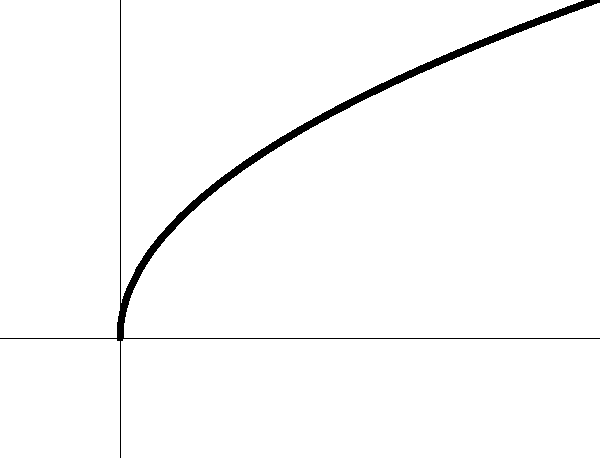
\includegraphics[width=0.3\textwidth]{fcv/number/yesqrtx}
  \end{center}
  \caption{The square root function.}
  \label{figure fcv number yesqrtx}
\end{figure}




\paragraph{A new mathematical constant.}
We cannot solve $x^2 = -1$ because the square root of $-1$ is not defined.  To
overcome this apparent shortcoming of the real number system, we
create a new symbolic constant $\sqrt{-1}$.  In performing arithmetic,
we will treat $\sqrt{-1}$ as we would a real constant like $\pi$ or a 
formal variable like $x$, i.e. $\sqrt{-1} + \sqrt{-1} = 2 \sqrt{-1}$.
This constant has the property:
$\left( \sqrt{-1} \right)^2 = -1$.  Now we can express the solutions
of $x^2 = -1$ as $x = \sqrt{-1}$ and $x = - \sqrt{-1}$.  These satisfy
the equation since $\left( \sqrt{-1} \right)^2 = -1$ and 
$\left( - \sqrt{-1} \right)^2 = (-1)^2 \left( \sqrt{-1} \right)^2 = -1$.
Note that we can express the square root of any negative real number in 
terms of $\sqrt{-1}$: $\sqrt{-r} = \sqrt{-1} \sqrt{r}$ for $r \geq 0$.  



\paragraph{Euler's notation.}
Euler introduced the notation of using the letter $i$ to denote $\sqrt{-1}$.
\index{i!Euler's notation}
\index{Euler's notation!i}
We will use the symbol $\imath$, an $i$ without a dot, to denote 
$\sqrt{-1}$.  This helps us distinguish it from $i$ used as a variable or 
index.%
\footnote{
  Electrical engineering types prefer to use $\jmath$ or $j$ to denote
  $\sqrt{-1}$.
  \index{j electrical engineering}
  }
We call any number of the form $\imath b$, 
$b \in \mathbb{R}$, a \textit{pure imaginary number}.%
\footnote{
  ``Imaginary'' is an unfortunate term.  Real numbers are 
  artificial; constructs of the mind.  Real numbers are no more real than
  imaginary numbers.
  }
\index{pure imaginary number}
\index{imaginary number}
Let $a$ and $b$ be real numbers.  The product of a real number and an 
imaginary number is an imaginary number: $(a)(\imath b) = \imath (a b)$.
The product of two imaginary numbers is a real number: 
$(\imath a)(\imath b) = - a b$.  However the sum of a real number and an 
imaginary number $a + \imath b$ is neither real nor imaginary.
We call numbers of the form $a + \imath b$ \textit{complex numbers}.%
\footnote{
  Here complex means ``composed of two or more parts'', not
  ``hard to separate, analyze, or solve''.  Those who disagree have a 
  complex number complex.
  }
\index{complex number}


\paragraph{The quadratic.}
Now we return to the quadratic with real coefficients, 
$x^2 + 2 a x + b = 0$.  It has the solutions
$x = -a \pm \sqrt{a^2 - b}$.  The solutions are real-valued
only if $a^2 - b \geq 0$.  If not, then we can define solutions as 
complex numbers.  
If the discriminant is negative, we write
$x = -a \pm \imath \sqrt{b - a^2}$.
Thus every quadratic polynomial with real coefficients has exactly 
two solutions, counting multiplicities.  
The fundamental theorem of algebra states that an $n^{\mathrm{th}}$
degree polynomial with complex coefficients has $n$, not necessarily
distinct, complex roots.  We will prove this result later using the 
theory of functions of a complex variable.





\paragraph{Component operations.}
Consider the complex number $z = x + \imath y$, $(x,y \in \mathbb{R})$.  
The \textit{real part} of $z$ is 
\index{real part}
$\Re(z) = x$; the \textit{imaginary part} of $z$ is $\Im(z) = y$.
\index{imaginary part}
Two complex numbers, $z = x + \imath y$ and $\zeta = \xi + \imath \psi$, are equal
if and only if $x = \xi$ and $y = \psi$.  The \textit{complex conjugate}%
\footnote{
  Conjugate: having features in common but opposite or inverse in 
  some particular.
  }
\index{complex conjugate}
of $z = x + \imath y$ is $\overline{z} \equiv x - \imath y$.  The notation 
$z^* \equiv x - \imath y$ is also used.


\paragraph{A little arithmetic.}
Consider two complex numbers: $z = x + \imath y$, $\zeta = \xi + \imath \psi$.
It is easy to express the sum or difference as a complex number.
\[
z + \zeta = (x + \xi) + \imath(y + \psi), \quad
z - \zeta = (x - \xi) + \imath(y - \psi)
\]
It is also easy to form the product.
\[
z \zeta = (x + \imath y)(\xi + \imath \psi)
= x \xi + \imath x \psi + \imath y \xi + \imath^2 y \psi
= (x \xi - y \psi) + \imath(x \psi + y \xi)
\]
The quotient is a bit more difficult.  (Assume that $\zeta$ is nonzero.)  How do
we express $z / \zeta = (x + \imath y) / (\xi + \imath \psi)$ as the sum of a real
number and an imaginary number?  The trick is to multiply the numerator and
denominator by the complex conjugate of $\zeta$.
\[
\frac{z}{\zeta} 
= \frac{x + \imath y}{\xi + \imath \psi}
= \frac{x + \imath y}{\xi + \imath \psi} \frac{\xi - \imath \psi}{\xi - \imath \psi}
= \frac{x \xi - \imath x \psi - \imath y \xi - \imath^2 y \psi}
{\xi^2 - \imath \xi \psi + \imath \psi \xi - \imath^2 \psi^2}
= \frac{(x \xi + y \psi) - \imath (x \psi + y \xi)}
{\xi^2 + \psi^2}
= \frac{(x \xi + y \psi)}{\xi^2 + \psi^2} - \imath \frac{x \psi + y \xi}{\xi^2 + \psi^2}
\]
Now we recognize it as a complex number.


\paragraph{Field properties.}
The set of complex numbers $\mathbb{C}$ form a field.  That essentially
means that we can do arithmetic with complex numbers.
When performing arithmetic, we simply treat $\imath$ as a symbolic 
constant with the property that $\imath^2 = -1$.
The field of complex numbers satisfy the following list of properties.
Each one is easy to verify; some are proved below.
(Let $z, \zeta, \omega \in \mathbb{C}$.)
\begin{enumerate}
\item
  Closure under addition and multiplication.
  \begin{align*}
    z + \zeta &= \left( x + \imath y \right) + \left(\xi + \imath \psi \right) 
    \\
    &= \left( x + \xi \right) + \imath \left( y + \psi \right) \in \mathbb{C} 
    \\
    z \zeta &= \left( x + \imath y \right) \left( \xi + \imath \psi \right) 
    \\
    &= x \xi + \imath x \psi + \imath y \xi + \imath^2 y \psi
    \\
    &= \left( x \xi - y \psi \right) 
    + \imath \left( x \psi + \xi y \right) \in \mathbb{C}
  \end{align*}
\item
  Commutativity of addition and multiplication.  $z + \zeta = \zeta + z$.
  $z \zeta = \zeta z$.
\item
  Associativity of addition and multiplication.  
  $\left( z + \zeta \right) + \omega = z + \left( \zeta  + \omega \right)$.
  $\left( z \zeta \right) \omega = z \left( \zeta \omega \right)$.
\item
  Distributive law.  $z \left( \zeta + \omega \right) = z \zeta + z \omega$.
\item
  Identity with respect to addition and multiplication.  Zero is the 
  additive identity element, $z + 0 = z$; unity is the muliplicative
  identity element, $z (1) = z$.
\item
  Inverse with respect to addition.
  $z + (-z)= (x + \imath y) + (- x - \imath y) = (x - x) + \imath(y - y) = 0$.
\item
  Inverse with respect to multiplication for nonzero numbers.
  $z z^{-1} = 1$, where 
  \[
  z^{-1} 
  = \frac{1}{z} 
  = \frac{1}{x + \imath y} 
  = \frac{1}{x + \imath y} \frac{x - \imath y}{x - \imath y} 
  = \frac{x - \imath y}{x^2 + y^2}
  = \frac{x}{x^2 + y^2} - \imath \frac{y}{x^2 + y^2}
  \]
\end{enumerate}





\paragraph{Properties of the complex conjugate.} 
\index{complex conjugate}
Using the field properties of complex numbers, we can derive 
the following properties of the complex conjugate, 
$\overline{z} = x - \imath y$.
\begin{enumerate}
\item
  $\displaystyle \overline{\left( \overline{z} \right)} = z$, 
\item
  $\displaystyle \overline{z + \zeta} = \overline{z} + \overline{\zeta}$, 
\item
  $\displaystyle \overline{z \zeta} = \overline{z} \overline{\zeta}$, 
\item
  $\displaystyle \overline{ \left( \frac{z}{\zeta} \right) } 
  = \frac{ \left( \overline{z} \right) }{ \left( \overline{\zeta} \right) }$. 
\end{enumerate}











%%=============================================================================
\section{The Complex Plane}





\paragraph{Complex plane.}
We can denote a complex number $z = x + \imath y$ as an ordered pair of real
numbers $(x,y)$.  Thus we can represent a complex number as a point in 
$\mathbb{R}^2$ where the first component is the real part and the second 
component is the imaginary part of $z$.  This is called the 
\textit{complex plane} 
\index{complex plane}
or the \textit{Argand diagram}.  (See Figure~\ref{complexplane}.)
\index{Argand diagram}
A complex number written as $z = x + \imath y$ is said to be in 
\textit{Cartesian form}, or \textit{$a + \imath b$ form}.
\index{Cartesian form}
\index{a + i b form}

\begin{figure}[h!]
  \begin{center}
    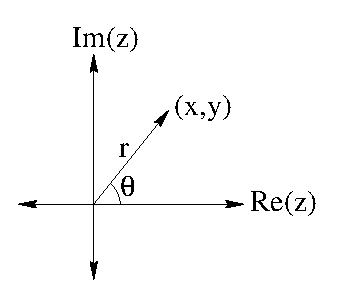
\includegraphics[width=0.25\textwidth]{fcv/number/comp_pln}
  \end{center}
  \caption{The complex plane.}
  \label{complexplane}
\end{figure}


Recall that there are two ways of describing a point in the complex plane: an
ordered pair of coordinates $(x, y)$ that give the horizontal and
vertical offset from the origin or the distance $r$ from the origin
and the angle $\theta$ from the positive horizontal axis.  The angle $\theta$
is not unique.  It is only determined up to an additive integer
multiple of $2 \pi$.




\paragraph{Modulus.}
The \textit{magnitude} or \textit{modulus} of a complex number is the 
\index{magnitude}
\index{modulus}
\index{complex number!magnitude}
\index{complex number!modulus}
distance of the point from the origin.  It is defined 
as $|z| = |x + \imath y| = \sqrt{x^2 + y^2}$.  Note that 
$z \overline{z} = (x + \imath y)(x - \imath y) = x^2 + y^2 = |z|^2$.
The modulus has the following properties.
\begin{enumerate}
\item
  $\displaystyle \left|z \zeta \right| = \left|z \right| \left|\zeta \right|$
\item
  $\displaystyle \left| \frac{z}{\zeta} \right| = \frac{ \left|z \right|}
  { \left|\zeta \right|}$ for $\zeta \neq 0$.
\item
  $\displaystyle \left|z + \zeta \right| \leq \left|z \right| + \left|\zeta \right|$
\item
  $\displaystyle \left|z + \zeta \right| 
  \geq \left|\left|z \right| - \left|\zeta \right| \right|$
\end{enumerate}
We could prove the first two properties by expanding in $x + \imath y$ form, 
but it would be fairly messy.  The proofs will become simple after polar 
form has been introduced.  The second two properties
follow from the triangle inequalities in geometry.  This will become apparent
after the relationship between complex numbers and vectors is introduced.
One can show that
\[
\left|z_1 z_2 \cdots z_n \right| 
= \left|z_1 \right| \left|z_2 \right| \cdots \left|z_n \right|
\]
and
\[
\left|z_1 + z_2 + \cdots + z_n \right| 
\leq \left|z_1 \right| + \left|z_2 \right| + \cdots + \left|z_n \right|
\]
with proof by induction.



\paragraph{Argument.}
The \textit{argument} of a complex number is the angle that the vector with
\index{argument!of a complex number}
tail at the origin and head at $z = x + \imath y$ makes with the positive 
$x$-axis.  The argument is denoted $\arg(z)$. 
Note that the argument is defined for all nonzero numbers and 
is only determined up to an additive integer multiple
of $2 \pi$.  That is, the argument of a complex number is the set of values:
$\{ \theta + 2 \pi n \mid n \in \mathbb{Z}\}$.  The \textit{principal argument}
\index{principal argument}
of a complex number is that angle in the set $\arg(z)$ which lies in the
range $(-\pi,\pi]$.  The principal argument is denoted $\Arg(z)$.
We prove the following identities in Exercise~\ref{exercise argument identities}.
\begin{gather*}
  \arg(z \zeta) = \arg(z) + \arg(\zeta) \\
  \Arg(z \zeta) \neq \Arg(z) + \Arg(\zeta) \\
  \arg\left( z^2 \right) = \arg(z) + \arg(z) \neq 2 \arg(z)
\end{gather*}



\begin{Example}
  Consider the equation $|z - 1 - \imath| = 2$.  The set of points satisfying 
  this equation
  is a circle of radius 2 and center at $1 + \imath$ in the complex plane.  You
  can see this by noting that $|z - 1 - \imath|$ is the distance from the point
  $(1,1)$.
  (See Figure~\ref{circ211}.)
  \begin{figure}[h!]
    \begin{center}
      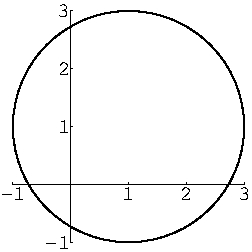
\includegraphics[width=0.3\textwidth]{fcv/number/circ211}
    \end{center}
    \caption{The solution is a circle.}
    \label{circ211}
  \end{figure}

  Another way to derive this is to substitute $z = x + \imath y$ 
  into the equation.
  \begin{gather*}
    |x + \imath y - 1 - \imath| = 2 
    \\
    \sqrt{(x-1)^2 + (y-1)^2} = 2 
    \\
    (x-1)^2 + (y-1)^2 = 4
  \end{gather*}
  This is the analytic geometry equation for a circle of radius 2 
  centered about $(1,1)$.  
\end{Example}







\begin{Example}
  Consider the curve described by 
  \[
  |z| + |z - 2| = 4.
  \]
  Note that $|z|$ is the distance from the origin in the complex plane and
  $|z - 2|$ is the distance from $z = 2$.  The equation is
  \[ 
  (\mathrm{distance from}\ (0,0)) + (\mathrm{distance from}\ (2,0)) = 4. 
  \]
  From geometry, we know that this is an ellipse with foci at $(0,0)$
  and $(2,0)$, major axis 2, and minor axis $\sqrt{3}$. 
  (See Figure~\ref{ellipse}.)
  \begin{figure}[h!]
    \begin{center}
      \includegraphics[width=0.3\textwidth]{fcv/number/ellipse}
    \end{center}
    \caption{The solution is an ellipse.}
    \label{ellipse}
  \end{figure}

  We can use the substitution $z = x + \imath y$ to get the equation in algebraic 
  form.
  \begin{gather*}
    |z| + |z - 2| = 4 
    \\
    |x + \imath y| + |x + \imath y - 2| = 4 
    \\
    \sqrt{x^2 + y^2} + \sqrt{(x - 2)^2 + y^2} = 4 
    \\
    x^2 + y^2 = 16 - 8 \sqrt{ (x - 2)^2 + y^2 } + x^2 - 4 x + 4 + y^2 
    \\
    x - 5 = -2 \sqrt{ (x - 2)^2 + y^2 } 
    \\
    x^2 - 10 x + 25 = 4 x^2 - 16 x + 16 + 4 y^2 
    \\
    \frac{1}{4} (x - 1)^2 + \frac{1}{3} y^2 = 1
  \end{gather*}
  Thus we have the standard form for an equation describing an ellipse.
\end{Example}






%%=============================================================================
\section{Polar Form}





\paragraph{Polar form.}
A complex number written in Cartesian form, $z = x + \imath y$,
can be converted \textit{polar form},
\index{polar form}
$z = r (\cos \theta + \imath \sin \theta)$, using trigonometry.
Here $r = |z|$ is the modulus and $\theta = \arctan(x,y)$ is 
the argument of $z$.  The argument is the angle between the $x$ axis and
the vector with its head at $(x,y)$.  (See Figure~\ref{polarfrm}.)
Note that $\theta$ is not unique.  If $z = r (\cos \theta + \imath \sin \theta)$ 
then $z = r (\cos (\theta + 2 n \pi) + \imath \sin (\theta + 2 n \pi) )$ for any
$n \in \mathbb{Z}$.

\begin{figure}[h!]
  \begin{center}
    \includegraphics[width=0.2\textwidth]{fcv/number/polarfrm}
  \end{center}
  \caption{Polar form.}
  \label{polarfrm}
\end{figure}




\paragraph{The arctangent.}
Note that $\arctan(x,y)$ is not the same thing as the old arctangent that
you learned about in trigonometry
$\arctan(x,y)$ is sensitive to the quadrant of the point $(x,y)$, while
$\arctan\left(\frac{y}{x} \right)$ is not.
For example,
\[
\arctan(1,1) = \frac{\pi}{4} + 2 n \pi \quad \mathrm{and} \quad
\arctan(-1,-1) = \frac{-3 \pi}{4} + 2 n \pi,
\]
whereas
\[
\arctan \left( \frac{-1}{-1} \right) = \arctan \left(\frac{1}{1} \right)
= \arctan(1).
\]




\paragraph{Euler's formula.}
\textit{Euler's formula}, $\e^{\imath \theta} = \cos \theta + \imath \sin \theta$,%
\footnote{
  See Exercise~\ref{exercise eulers formula} for justification of 
  Euler's formula.
  }
\index{Euler's formula}
allows us to write the polar form more compactly.  Expressing 
the polar form in terms of the exponential function of imaginary argument
makes arithmetic with complex numbers much more convenient.
\[
z = r (\cos \theta + \imath \sin \theta) = r \e^{\imath \theta}
\]
The exponential of an imaginary argument has all the nice properties that
we know from studying functions of a real variable, like
$\e^{\imath a} \e^{\imath b} = \e^{\imath(a + b)}$.  Later on we will 
introduce the exponential of a complex number.

Using Euler's Formula, we can express the cosine and sine in terms of the
exponential.
\begin{gather*}
  \frac{\e^{\imath \theta} + \e^{-\imath \theta}}{2}
  = \frac{(\cos(\theta) + \imath \sin(\theta)) + (\cos(-\theta) + \imath \sin(-\theta))}{2}
  = \cos(\theta)
  \\
  \frac{\e^{\imath \theta} - \e^{-\imath \theta}}{\imath 2}
  = \frac{(\cos(\theta) + \imath \sin(\theta)) - (\cos(-\theta) + \imath \sin(-\theta))}{\imath 2}
  = \sin(\theta)
\end{gather*}






\paragraph{Arithmetic with complex numbers.}
Note that it is convenient to add complex numbers in Cartesian form.
\[
z + \zeta
= \left( x + \imath y \right) + \left( \xi + \imath \psi \right) 
= \left( x + \xi \right) + \imath \left( y + \psi \right)
\]
However, it is difficult to multiply or divide them in Cartesian form.
\begin{gather*}
  z \zeta
  = \left( x + \imath y \right)  \left( \xi + \imath \psi \right) 
  = \left( x \xi - y \psi \right) + \imath \left( x \psi + \xi y \right)
  \\
  \frac{z}{\zeta}
  = \frac{x + \imath y}{\xi + \imath \psi}
  = \frac{\left( x + \imath y \right)  \left( \xi - \imath \psi \right)}
  {\left( \xi + \imath \psi \right)  \left( \xi - \imath \psi \right)}
  = \frac{x \xi + y \psi}{\xi^2 + \psi^2}
  + \imath \frac{\xi y - x \psi}{\xi^2 + \psi^2}
\end{gather*}
On the other hand, it is difficult to add complex numbers in polar form.
\begin{align*}
  z + \zeta
  &= r \e^{\imath \theta} + \rho \e^{\imath \phi}
  \\
  &= r \left( \cos \theta + \imath \sin \theta \right) 
  + \rho \left( \cos \phi + \imath \sin \phi \right) 
  \\
  &= r \cos \theta + \rho \cos \phi
  + \imath \left( r \sin \theta + \rho \sin \phi \right) 
  \\
  &= \sqrt{ \left( r \cos \theta + \rho \cos \phi \right)^2
    + \left( r \sin \theta + \rho \sin \phi \right)^2 } 
  \\
  &\qquad \times \e^{\imath \arctan \left( 
      r \cos \theta + \rho \cos \phi, 
      r \sin \theta + \rho \sin \phi \right)} 
  \\
  &= \sqrt{ r^2 + \rho^2 + 2 \cos \left( \theta - \phi \right) }
  \e^{\imath \arctan \left( 
      r \cos \theta + \rho \cos \phi,
      r \sin \theta + \rho \sin \phi \right)} 
\end{align*}
However, it is convenient to multiply and divide them in polar form.
\begin{gather*}
  z \zeta
  = r \e^{\imath \theta} \rho \e^{\imath \phi} = r \rho \e^{\imath \left( \theta + \phi \right)}
  \\
  \frac{z}{\zeta}
  = \frac{r \e^{\imath \theta}}{\rho \e^{\imath \phi}}
  = \frac{r}{\rho} \e^{\imath \left( \theta - \phi \right)}
\end{gather*}
Keeping this in mind will make working with complex numbers a shade or 
two less grungy.






\begin{Result}
  \label{cartesian_and_polar_form}
  Euler's formula is 
  \[
  \e^{\imath \theta} = \cos \theta + \imath \sin \theta.
  \]
  We can write the cosine and sine in terms of the exponential.
  \[
  \cos(\theta) = \frac{\e^{\imath \theta} + \e^{-\imath \theta}}{2}, 
  \qquad
  \sin(\theta) = \frac{\e^{\imath \theta} - \e^{-\imath \theta}}{\imath 2}
  \]
  To change between Cartesian and polar form, use the identities
  \begin{align*}
    r \e^{\imath \theta} &= r \cos \theta + \imath r \sin \theta, 
    \\
    x + \imath y &= \sqrt{x^2 + y^2} \e^{\imath \arctan(x,y)}.
  \end{align*}
  Cartesian form is convenient for addition.  Polar form is convenient 
  for multiplication and division.
\end{Result}







\begin{Example}
  We write $5 + \imath 7$ in polar form.
  \[
  5 + \imath 7 = \sqrt{74} \e^{\imath \arctan(5,7) }
  \]
  We write $2 \e^{\imath \pi / 6}$ in Cartesian form.
  \begin{align*}
    2 \e^{\imath \pi / 6} 
    &= 2 \cos \left( \frac{\pi}{6} \right) 
    + 2 \imath \sin \left( \frac{\pi}{6} \right) 
    \\
    &= \sqrt{3} + \imath
  \end{align*}
\end{Example}








\begin{Example}
  We will prove the trigonometric identity
  \[
  \cos^4 \theta = \frac{1}{8} \cos(4 \theta) +
  \frac{1}{2} \cos(2 \theta) + \frac{3}{8}.
  \]
  We start by writing the cosine in terms of the exponential.
  \begin{align*}
    \cos^4 \theta   
    &=  \left(\frac{\e^{\imath \theta} + \e^{-\imath \theta}}{2}\right)^4 
    \\
    &=  \frac{1}{16} \left( \e^{\imath 4 \theta} + 4 \e^{\imath 2 \theta} + 6 +
    4 \e^{-\imath 2 \theta} + \e^{-\imath 4 \theta} \right) 
    \\
    &=  \frac{1}{8} \left( \frac{\e^{\imath 4 \theta} + \e^{-\imath 4 \theta}}{2} \right) +
    \frac{1}{2} \left( \frac{\e^{\imath 2 \theta} + \e^{-\imath 2 \theta}}{2} \right) + \frac{3}{8} 
    \\
    &=  \frac{1}{8} \cos(4 \theta) + \frac{1}{2} \cos(2 \theta) + \frac{3}{8}
  \end{align*}
\end{Example}











By the definition of exponentiation, we have $\e^{\imath n \theta} = \left( \e^{\imath \theta} \right)^n$
We apply Euler's formula to obtain a result which is useful in deriving
trigonometric identities.
\[
\cos(n \theta) + \imath \sin(n \theta) = (\cos \theta + \imath \sin \theta)^n
\]


\begin{Result}
  \label{demoivres_theorem}
  \textbf{DeMoivre's Theorem.}%
  \footnote{It's amazing what passes for a theorem these days.  
    I would think that this would be a corollary at most.}
  \[
  \cos(n \theta) + \imath \sin(n \theta) = (\cos \theta + \imath \sin \theta)^n
  \]
\end{Result}










\begin{Example}
  We will express $\cos(5 \theta)$ in terms of $\cos \theta$ and 
  $\sin(5 \theta)$ in terms of $\sin \theta$.
  We start with DeMoivre's theorem.
  \[
  \e^{\imath 5 \theta} = \left( \e^{\imath \theta} \right)^5
  \]
  \begin{align*}
    \cos(5 \theta) + \imath \sin(5 \theta)
    &= (\cos \theta + \imath \sin \theta)^5 
    \\
    &= \binom{5}{0} \cos^5 \theta
    + \imath \binom{5}{1} \cos^4 \theta \sin \theta
    - \binom{5}{2} \cos^3 \theta \sin^2 \theta
    - \imath \binom{5}{3} \cos^2 \theta \sin^3 \theta 
    \\
    & \qquad + \binom{5}{4} \cos \theta \sin^4 \theta
    + \imath \binom{5}{5} \sin^5 \theta 
    \\
    &= \left( \cos^5 \theta - 10 \cos^3 \theta \sin^2 \theta + 5 \cos \theta \sin^4 \theta \right)
    + \imath \left( 5 \cos^4 \theta \sin \theta - 10 \cos^2 \theta \sin^3 \theta + \sin^5 \theta \right)
  \end{align*}
  Then we equate the real and imaginary parts.
  \begin{align*}
    \cos(5 \theta) 
    &= \cos^5 \theta - 10 \cos^3 \theta \sin^2 \theta
    + 5 \cos \theta \sin^4 \theta 
    \\
    \sin(5 \theta) &= 5 \cos^4 \theta \sin \theta - 10  \cos^2 \theta \sin^3 \theta + \sin^5 \theta
  \end{align*}
  Finally we use the Pythagorean identity, $\cos^2 \theta + \sin^2 \theta = 1$.
  \begin{gather*} 
    \cos(5 \theta) = \cos^5 \theta - 10 \cos^3 \theta \left( 1 - \cos^2 \theta \right)
    + 5 \cos \theta \left( 1 - \cos^2 \theta \right)^2  
    \\
    \boxed{ 
      \cos(5 \theta) = 16 \cos^5 \theta - 20 \cos^3 \theta + 5 \cos \theta 
      } 
    \\
    \sin(5 \theta) = 5 \left( 1 - \sin^2 \theta \right)^2 \sin \theta 
    - 10 \left( 1 - \sin^2 \theta \right) \sin^3 \theta + \sin^5 \theta
    \\
    \boxed{ 
      \sin(5 \theta) = 16 \sin^5 \theta - 20 \sin^3 \theta + 5 \sin \theta
      } 
  \end{gather*}
\end{Example}
















%%=============================================================================
\section{Arithmetic and Vectors}
\index{complex numbers!arithmetic}
\index{complex numbers!vectors}





\paragraph{Addition.}
We can represent the complex number $z = x + \imath y = r \e^{\imath \theta}$ as 
a vector in Cartesian space with tail at the origin and head at 
$(x,y)$, or equivalently, the vector of length $r$ and angle $\theta$.
With the vector representation, we can add complex numbers by connecting
the tail of one vector to the head of the other.  The vector $z + \zeta$
is the diagonal of the parallelogram defined by $z$ and $\zeta$.
(See Figure~\ref{add_neg_mult}.)




\paragraph{Negation.}
The negative of $z = x + \imath y$ is $- z = - x - \imath y$.  In polar form we have
$z = r \e^{\imath \theta}$ and $- z = r \e^{\imath (\theta + \pi)}$, (more 
generally, $z = r \e^{\imath (\theta + (2 n+1) \pi)}$, $n \in \mathbb{Z}$.
In terms of vectors, $- z$ has the same magnitude but opposite direction 
as $z$.  (See Figure~\ref{add_neg_mult}.)





\paragraph{Multiplication.}
The product of $z = r \e^{\imath \theta}$ and $\zeta = \rho \e^{\imath \phi}$ is
$z \zeta = r \rho \e^{\imath (\theta + \phi)}$.  The length of the vector
$z \zeta$ is the product of the lengths of $z$ and $\zeta$.  The 
angle of $z \zeta$ is the sum of the angles of $z$ and $\zeta$.
(See Figure~\ref{add_neg_mult}.)

Note that $\arg(z \zeta) = \arg(z) + \arg(\zeta)$.  Each of these arguments
has an infinite number of values.  If we write out the multi-valuedness
explicitly, we have
\[
\{ \theta + \phi + 2 \pi n : n \in \mathbb{Z} \} =
\{ \theta + 2 \pi n : n \in \mathbb{Z} \}
+ \{ \phi + 2 \pi n : n \in \mathbb{Z} \}
\]
The same is not true of the principal argument.  In general,
$\Arg(z \zeta) \neq \Arg(z) + \Arg(\zeta)$.  Consider the case 
$z = \zeta = \e^{\imath 3 \pi / 4}$.  Then $\Arg(z) = \Arg(\zeta) = 3 \pi / 4$,
however, $\Arg(z \zeta) = - \pi / 2$.

\begin{figure}[h!]
  \begin{center}
      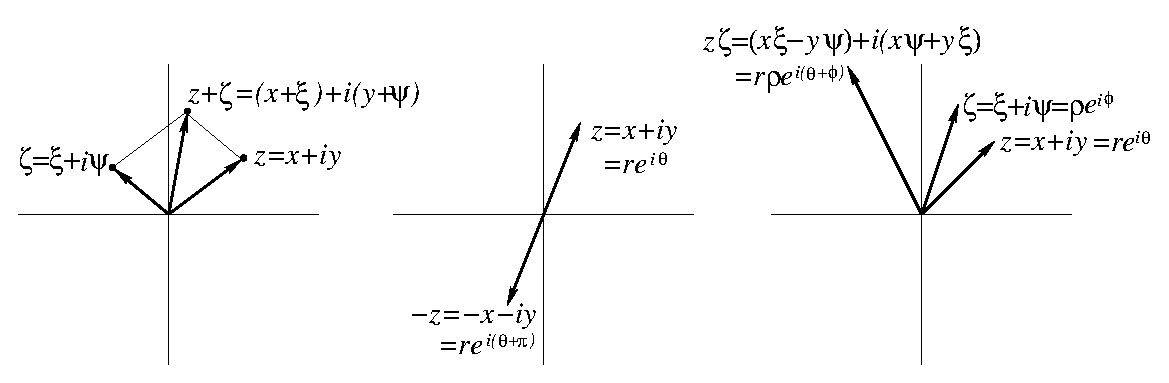
\includegraphics[width=\textwidth]{fcv/number/add_neg_mult}
  \end{center}
  \caption{Addition, negation and multiplication.}
  \label{add_neg_mult}
\end{figure}







\paragraph{Multiplicative inverse.}
Assume that $z$ is nonzero.  The multiplicative inverse of 
$z = r \e^{\imath \theta}$ is $\frac{1}{z} = \frac{1}{r} \e^{-\imath \theta}$.
The length of $\frac{1}{z}$ is the multiplicative inverse of the length
of $z$.  The angle of $\frac{1}{z}$ is the negative of the angle of $z$.
(See Figure~\ref{inv_div_conj}.)







\paragraph{Division.}
Assume that $\zeta$ is nonzero.
The quotient of $z = r \e^{\imath \theta}$ and $\zeta = \rho \e^{\imath \phi}$ is
$\frac{z}{\zeta} = \frac{r}{\rho} \e^{ \imath (\theta - \phi)}$.  The length of 
the vector $\frac{z}{\zeta}$ is the quotient of the lengths of 
$z$ and $\zeta$.  The angle of $\frac{z}{\zeta}$ is the difference of the 
angles of $z$ and $\zeta$.
(See Figure~\ref{inv_div_conj}.)





\paragraph{Complex conjugate.}
The complex conjugate of $z = x + \imath y = r \e^{\imath \theta}$ is 
$\overline{z} = x - \imath y = r \e^{-\imath \theta}$.  $\overline{z}$ is the mirror image of
$z$, reflected across the $x$ axis.  In other words, $\overline{z}$ has the
same magnitude as $z$ and the angle of $\overline{z}$ is the negative of 
the angle of $z$.
(See Figure~\ref{inv_div_conj}.)

\begin{figure}[h!]
  \begin{center}
      \includegraphics[width=\textwidth]{fcv/number/inv_div_conj}
  \end{center}
  \caption{Multiplicative inverse, division and complex conjugate.}
  \label{inv_div_conj}
\end{figure}

















%%=============================================================================
\section{Integer Exponents}





Consider the product $(a + b)^n$, $n \in \mathbb{Z}$.  
If we know $\arctan(a,b)$ then 
it will be most convenient to expand the product working in polar form.  
If not, we can write $n$ in base 2 to efficiently do the multiplications.




\begin{Example}
  Suppose that we want to write $\left( \sqrt{3} + \imath \right)^{20}$ 
  in Cartesian form.%
  \footnote{No, I have no idea why we would want to do that.  Just humor
    me.  If you pretend that you're interested, I'll do the same.  Believe
    me, expressing your real feelings here isn't going to do anyone any good.}
  We can do the multiplication directly.  Note that $20$ is $10100$ in base 2.
  That is, $20 = 2^4 + 2^2$.  We first calculate the powers of the form
  $\left( \sqrt{3} + \imath \right)^{2^n}$ by successive squaring.
  \begin{align*}
    \left( \sqrt{3} + \imath \right)^2 &= 2 + \imath 2 \sqrt{3} \\
    \left( \sqrt{3} + \imath \right)^4 &= -8 + \imath 8 \sqrt{3} \\
    \left( \sqrt{3} + \imath \right)^8 &= -128 - \imath 128 \sqrt{3} \\
    \left( \sqrt{3} + \imath \right)^{16} &= -32768 + \imath 32768 \sqrt{3} 
  \end{align*}
  Next we multiply $\left( \sqrt{3} + \imath \right)^4$ and 
  $\left( \sqrt{3} + \imath \right)^{16}$ to obtain the answer.
  \[
  \left( \sqrt{3} + \imath \right)^{20} 
  = \left( -32768 + \imath 32768 \sqrt{3} \right) 
  \left( - 8 + \imath 8 \sqrt{3} \right)
  = - 524288 - \imath 524288 \sqrt{3}
  \]

  Since we know that $\arctan\left( \sqrt{3},1 \right) = \pi/6$,
  it is easiest to do this problem by first changing to modulus-argument form.
  \begin{align*}
    \left( \sqrt{3} + \imath \right)^{20} 
    &= \left( \sqrt{ \left( \sqrt{3} \right)^2 + 1^2} 
      \e^{\imath \arctan(\sqrt{3},1)} \right)^{20} 
    \\
    &= \left( 2 \e^{\imath \pi / 6} \right)^{20} 
    \\
    &= 2^{20} \e^{\imath 4 \pi / 3} 
    \\
    &= 1048576 \left( - \frac{1}{2} - \imath \frac{\sqrt{3}}{2} \right) 
    \\
    &= - 524288 - \imath 524288 \sqrt{3}
  \end{align*}
\end{Example}








\begin{Example}
  Consider $(5 + \imath 7)^{11}$.  We will do the exponentiation in polar form and
  write the result in Cartesian form.
  \begin{align*}
    (5 + \imath 7)^{11}
    &= \left( \sqrt{74} \e^{\imath \arctan(5,7)} \right)^{11} \\
    &= 74^5 \sqrt{74} ( \cos( 11 \arctan(5,7)) 
    + \imath \sin( 11 \arctan(5,7)))\\
    &= 2219006624 \sqrt{74} \cos( 11 \arctan(5,7))
    + \imath 2219006624 \sqrt{74} \sin( 11 \arctan(5,7))
  \end{align*}
  The result is correct, but not very satisfying.
  This expression could be simplified.
  You could evaluate the trigonometric functions with some fairly messy
  trigonometric identities.  This would take much more work than directly 
  multiplying $(5 + \imath 7)^{11}$.
\end{Example}












%%=============================================================================
\section{Rational Exponents}





In this section we consider complex numbers with rational exponents,
$z^{p/q}$, where $p/q$ is a rational number.  First we consider unity 
raised to the $1/n$ power.   We define $1^{1/n}$ as the set of numbers
$\{z\}$ such that $z^n = 1$.
\[
1^{1/n} = \left\{ z \mid z^n = 1 \right\}
\]
We can find these values by writing $z$ in modulus-argument form.
\begin{gather*}
  z^n = 1 
  \\
  r^n \e^{\imath n \theta} = 1 
  \\
  r^n = 1 \qquad n \theta = 0 \mod 2 \pi 
  \\
  r = 1 \qquad \theta = 2 \pi k\ \mathrm{for}\ k \in \mathbb{Z}
  \\
  1^{1/n} = \left\{ \e^{\imath 2 \pi k/n} \mid k \in \mathbb{Z} \right\} 
\end{gather*}
There are only $n$ distinct values as a result of the $2 \pi$ periodicity 
of $\e^{\imath \theta}$. $\e^{\imath 2 \pi} = \e^{\imath 0}$.
\[
1^{1/n} = \left\{ \e^{\imath 2 \pi k / n} \mid k = 0, \ldots, n-1 \right\}
\]
These values are equally spaced points on the unit circle in the 
complex plane.



\begin{Example}
  $1^{1/6}$ has the 6 values,
  \[
  \left\{ \e^{\imath 0}, \e^{\imath \pi/3}, \e^{\imath 2 \pi/3}, \e^{\imath \pi}, \e^{\imath 4 \pi/3},
    \e^{\imath 5 \pi/3} \right\}.
  \]
  In Cartesian form this is
  \[
  \left\{ 1, \frac{1 + \imath \sqrt{3}}{2}, \frac{-1 + \imath \sqrt{3}}{2},
    -1, \frac{-1 - \imath \sqrt{3}}{2}, \frac{1 - \imath \sqrt{3}}{2} \right\}.
  \]
  The sixth roots of unity are plotted in Figure~\ref{sixth_roots}.
  \begin{figure}[h!]
    \begin{center}
        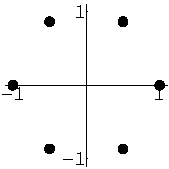
\includegraphics[width=0.2\textwidth]{fcv/number/sixth_roots}
    \end{center}
    \caption{The sixth roots of unity.}
    \label{sixth_roots}
  \end{figure}
\end{Example}




The $n^{\mathrm{th}}$ roots of the complex number $c = \alpha \e^{\imath \beta}$
are the set of numbers $z = r \e^{\imath \theta}$ such that
\begin{gather*}
  z^n = c = \alpha \e^{\imath \beta} 
  \\
  r^n \e^{\imath n \theta} = \alpha \e^{\imath \beta} 
  \\
  r = \sqrt[n]{\alpha} \qquad n \theta = \beta \mod 2 \pi 
  \\
  r = \sqrt[n]{\alpha} \qquad \theta = (\beta + 2 \pi k) / n\ \mathrm{for}\ 
  k = 0, \ldots, n - 1.
\end{gather*}
Thus 
\[
c^{1/n} = \left\{ \sqrt[n]{\alpha} \e^{\imath (\beta + 2 \pi k) / n } \mid k = 0, \ldots, n - 1 \right\}
= \left\{ \sqrt[n]{|c|} \e^{\imath (\Arg(c) + 2 \pi k) / n } \mid k = 0, \ldots, n - 1 \right\}
\]


\paragraph{Principal roots.}
The \textit{principal $n^{\mathrm{th}}$ root} is denoted
\index{principal root}
\[
\sqrt[n]{z} \equiv \sqrt[n]{z} \e^{\imath \Arg(z) / n}.
\]
Thus the principal root has the property
\[
- \pi / n < \Arg \left( \sqrt[n]{z} \right) \leq \pi / n.
\]
This is consistent with the notation from functions of a real variable:
$\sqrt[n]{x}$ denotes the positive $n^{\mathrm{th}}$ root of a positive 
real number.  We adopt the convention that $z^{1/n}$ denotes the 
$n^{\mathrm{th}}$ roots of $z$, which is a set of $n$ numbers and 
$\sqrt[n]{z}$ is the principal $n^{\mathrm{th}}$ root of $z$, which is a 
single number.  
The $n^{\mathrm{th}}$ roots of $z$ are the principal $n^{\mathrm{th}}$
root of $z$ times the $n^{\mathrm{th}}$ roots of unity.
\begin{gather*}
  z^{1/n} = \left\{ \sqrt[n]{r} \e^{\imath (\Arg(z) + 2 \pi k) / n } \mid k = 0, \ldots, n-1 \right\} 
  \\
  z^{1/n} = \left\{ \sqrt[n]{z} \e^{\imath 2 \pi k / n } \mid k = 0, \ldots, n-1 \right\} 
  \\
  z^{1/n} = \sqrt[n]{z} 1^{1/n}
\end{gather*}




\paragraph{Rational exponents.}
We interpret $z^{p/q}$ to mean $z^{(p/q)}$.  That is, we first simplify
the exponent, i.e. reduce the fraction,  before carrying out the 
exponentiation.  Therefore $z^{2/4} = z^{1/2}$ and $z^{10/5} = z^2$.
If $p/q$ is a reduced fraction, ($p$ and $q$ are relatively prime, in other
words, they have no common factors), then 
\[
z^{p/q} \equiv \left( z^p \right)^{1/q}.
\]
Thus $z^{p/q}$ is a set of $q$ values.  Note that for an un-reduced fraction
$r/s$, 
\[
\left( z^r \right)^{1/s} \neq \left( z^{1/s} \right)^r.
\]
The former expression is a set of $s$ values while the latter is a set of
no more that $s$ values.  For instance, $\left( 1^2 \right)^{1/2} = 1^{1/2} = \pm 1$
and $\left( 1^{1/2} \right)^2 = (\pm 1)^2 = 1$.






\begin{Example}
  Consider $2^{1/5}$, $(1 + \imath)^{1/3}$ and $(2 + \imath)^{5/6}$.
  \[
  2^{1/5} = \sqrt[5]{2} \e^{\imath 2 \pi k / 5}, \quad \mathrm{for}\ k = 0,1,2,3,4
  \]
  \begin{align*}
    (1 + \imath)^{1/3}
    &= \left( \sqrt{2} \e^{\imath \pi/4} \right)^{1/3} 
    \\
    &= \sqrt[6]{2} \e^{\imath \pi / 12} \e^{\imath 2 \pi k / 3}, \quad \mathrm{for}\ k = 0, 1, 2
  \end{align*}
  \begin{align*}
    (2 + \imath)^{5/6}
    &= \left( \sqrt{5} \e^{\imath \Arctan(2,1) } \right)^{5/6} 
    \\
    &= \left( \sqrt{5^5} \e^{\imath 5 \Arctan(2,1) } \right)^{1/6} 
    \\
    &= \sqrt[12]{5^5} \e^{\imath \frac{5}{6} \Arctan(2,1)}
    \e^{\imath \pi k / 3}, \quad \mathrm{for}\ k = 0,1,2,3,4,5
  \end{align*}
\end{Example}





\begin{Example}
  We find the roots of $z^5 + 4$.
  \begin{align*}
    (- 4)^{1/5}
    &= \left( 4 \e^{\imath \pi} \right)^{1/5} 
    \\
    &= \sqrt[5]{4} \e^{\imath \pi (1 + 2 k) / 5}, \quad \mathrm{for}\ k = 0,1,2,3,4
  \end{align*}
\end{Example}













\raggedbottom
%%=============================================================================
\exercises{
\pagebreak
\flushbottom
\section{Exercises}




%%-----------------------------------------------------------------------------
\begin{large}
  \noindent
  \textbf{Complex Numbers}
\end{large}





\begin{Exercise}
  \label{exercise 1i27}
  If $z = x + \imath y$, write the following in the form $a + \imath b$:
  \begin{enumerate}
  \item
    $\displaystyle
    (1 + \imath 2)^7
    $
  \item
    $\displaystyle
    \frac{1}{ \left( \overline{z} \overline{z} \right) }
    $
  \item
    $\displaystyle
    \frac{ \imath z + \overline{z} }{ (3 + \imath)^9 }
    $
  \end{enumerate}

  \hintsolution{1i27}
\end{Exercise}







%% \frac{1 + \imath 2}{3 - \imath 4} + \frac{2-\imath}{\imath 5} = - \frac{2}{5}
\begin{Exercise}
  \label{exercise (1 - i)4 = -4}
  Verify that:
  \begin{enumerate}
  \item
    $\displaystyle \frac{1 + \imath 2}{3 - \imath 4} + \frac{2 - \imath}{\imath 5} 
    = - \frac{2}{5}$
  \item
    $\displaystyle (1 - \imath)^4 = - 4$
  \end{enumerate}

  \hintsolution{(1 - i)4 = -4}
\end{Exercise}






%% \left( 1 + \imath \sqrt{3} \right)^{-10}
\begin{Exercise}
  \label{exercise (11 + i4)2}
  Write the following complex numbers in the form $a + \imath b$.
  \begin{enumerate}
  \item
    $\displaystyle \left( 1 + \imath \sqrt{3} \right)^{-10}$
  \item
    $\displaystyle (11 + \imath 4)^2$
  \end{enumerate}

  \hintsolution{(11 + i4)2}
\end{Exercise}





%% \left( \frac{2 + \imath}{\imath 6 - (1 - \imath 2)} \right)^2
\begin{Exercise}
  \label{exercise (1 - i)7}
  Write the following complex numbers in the form $a + \imath b$
  \begin{enumerate}
  \item
    $\displaystyle
    \left( \frac{2 + \imath}{\imath 6 - (1 - \imath 2)} \right)^2
    $
  \item
    $\displaystyle
    (1 - \imath)^7
    $
  \end{enumerate}

  \hintsolution{(1 - i)7}
\end{Exercise}








%% \overline{ \left( \frac{ \overline{z} }{ z } \right) }$
\begin{Exercise}
  \label{exercise ov ov z z}
  If $z = x + \imath y$, write the following in the form $u(x,y) + \imath v(x,y)$.
  \begin{enumerate}
  \item
    $\displaystyle 
    \overline{ \left( \frac{ \overline{z} }{ z } \right) }
    $
  \item
    $\displaystyle 
    \frac{ z + \imath 2 }{ 2 - \imath \overline{z} }
    $
  \end{enumerate}

  \hintsolution{ov ov z z}
\end{Exercise}







%% Quaternions are sometimes used as a generalization of complex numbers.
\begin{Exercise}
  \label{exercise quaternion}
  Quaternions are sometimes used as a generalization of complex numbers.
  A quaternion $u$ may be defined as
  \[
  u = u_0 + \imath u_1 + \jmath u_2 + k u_3
  \]
  where $u_0$, $u_1$, $u_2$ and $u_3$ are real numbers and $\imath$, $\jmath$ and $k$
  are objects which satisfy
  \[
  \imath^2 = \jmath^2 = k^2 = -1, \quad
  \imath \jmath = k, \quad
  \jmath \imath = - k
  \]
  and the usual associative and distributive laws.  Show that for any
  quaternions $u$, $w$ there exists a quaternion $v$ such that
  \[
  u v = w
  \]
  except for the case $u_0 = u_1 = u_2 = u_3$.

  \hintsolution{quaternion}
\end{Exercise}






%% $\alpha = t\beta$ $\Im(\alpha\overline{\beta}) = 0$
\begin{Exercise}
  \label{exercise alpha = t beta}
  Let $\alpha \neq 0$, $\beta \neq 0$ be two complex numbers.
  Show that $\alpha = t \beta$ for some real number $t$ (i.e. the vectors
  defined by $\alpha$ and $\beta$ are parallel) if and only if
  $\Im\left( \alpha \overline{\beta} \right) = 0$.

  \hintsolution{alpha = t beta}
\end{Exercise}







%%-----------------------------------------------------------------------------
\begin{large}
  \noindent
  \textbf{The Complex Plane}
\end{large}




\begin{Exercise}
  \label{exercise 1i13}
  Find and depict all values of
  \begin{enumerate}
  \item
    $\displaystyle
    (1 + \imath)^{1/3}
    $
  \item
    $\displaystyle
    \imath^{1/4}
    $
  \end{enumerate}
  Identify the principal root.

  \hintsolution{1i13}
\end{Exercise}






\begin{Exercise}
  \label{exercise Rez+2Imz1}
  Sketch the regions of the complex plane:
  \begin{enumerate}
  \item
    $\displaystyle
    | \Re(z) | + 2 | \Im(z) | \leq 1
    $
  \item
    $\displaystyle
    1 \leq |z - \imath| \leq 2
    $
  \item
    $\displaystyle
    |z - \imath| \leq |z + \imath|
    $
  \end{enumerate}

  \hintsolution{Rez+2Imz1}
\end{Exercise}








%% argument identities
\begin{Exercise}
  \label{exercise argument identities}
  Prove the following identities.
  \begin{enumerate}
  \item
    $\arg(z \zeta) = \arg(z) + \arg(\zeta)$
  \item
    $\Arg(z \zeta) \neq \Arg(z) + \Arg(\zeta)$
  \item
    $\arg \left( z^2 \right) = \arg(z) + \arg(z) \neq 2 \arg(z)$
  \end{enumerate}

  \hintsolution{argument identities}
\end{Exercise}




%% triangle inequalities
\begin{Exercise}
  \label{exercise triangle inequalities}
  Show, both by geometric and algebraic arguments, that
  for complex numbers $z$ and $\zeta$ the inequalities
  \[
  ||z|-|\zeta||\leq |z + \zeta|\leq |z| + |\zeta|
  \]
  hold.

  \hintsolution{triangle inequalities}
\end{Exercise}





%% $(-1)^{-3/4}$ $8^{1/6}$
\begin{Exercise}
  \label{exercise -1 -3/4 8 1/6}
  Find all the values of
  \begin{enumerate}
  \item
    $(- 1)^{-3/4}$
  \item
    $8^{1/6}$
  \end{enumerate}
  and show them graphically.

  \hintsolution{-1 -3/4 8 1/6}
\end{Exercise}







%% (-1)^{-1/4}
\begin{Exercise}
  \label{exercise 16 1/8}
  Find all values of
  \begin{enumerate}
  \item
    $ \displaystyle
    (- 1)^{-1/4}
    $
  \item
    $ \displaystyle
    16^{1/8}
    $
  \end{enumerate}
  and show them graphically.

  \hintsolution{16 1/8}
\end{Exercise}



%% $1 < |z - 2 \imath| < 2$ $| \Re(z) | + 5 | \Im(z) | = 1$
\begin{Exercise}
  \label{exercise 1 z-i2 2}
  Sketch the regions or curves described by
  \begin{enumerate}
  \item
    $\displaystyle
    1 < |z - \imath 2| < 2
    $
  \item
    $\displaystyle
    | \Re(z) | + 5 | \Im(z) | = 1
    $
  \item
    $\displaystyle
    |z - \imath|=|z + \imath|
    $
  \end{enumerate}

  \hintsolution{1 z-i2 2}
\end{Exercise}




%% |z - 1 + \imath|\leq 1
\begin{Exercise}
  \label{exercise z-1+i 1}
  Sketch the regions or curves described by
  \begin{enumerate}
  \item
    $\displaystyle
    |z - 1 + \imath|\leq 1
    $
  \item
    $\displaystyle
    \Re(z)- \Im(z) = 5
    $
  \item
    $\displaystyle
    |z - \imath| + |z + \imath| = 1
    $
  \end{enumerate}

  \hintsolution{z-1+i 1}
\end{Exercise}





%% |\e^{\imath \theta}-1| =2
\begin{Exercise}
  \label{exercise e i theta - 1 = 2}
  Solve the equation
  \[
  |\e^{\imath \theta}-1| = 2
  \]
  for $\theta$ ($0 \leq \theta \leq \pi$) and verify the solution geometrically.

  \hintsolution{e i theta - 1 = 2}
\end{Exercise}






%%-----------------------------------------------------------------------------
\begin{large}
  \noindent
  \textbf{Polar Form}
\end{large}



%% Euler's formula
\begin{Exercise}
  \label{exercise eulers formula}
  Show that Euler's formula, $\e^{\imath \theta} = \cos \theta + \imath \sin \theta$, is
  formally consistent with the standard Taylor series expansions for
  the real functions $\e^x$, $\cos x$ and $\sin x$.  Consider the
  Taylor series of $\e^x$ about $x = 0$ to be the definition of the
  exponential function for complex argument.

  \hintsolution{eulers formula}
\end{Exercise}





%% \cos(3\theta) = \cos^3(\theta) -3\cos(\theta)\sin^2(\theta).
\begin{Exercise}
  \label{exercise cos 3t = cos3 t - 3 cos t sin2 t}
  Use de Moivre's formula to derive the 
  trigonometric identity
  \[
  \cos(3 \theta) = \cos^3(\theta) - 3 \cos(\theta) \sin^2(\theta).
  \]

  \hintsolution{cos 3t = cos3 t - 3 cos t sin2 t}
\end{Exercise}







%% 1 + z + z^2 + \cdots + z^n = \frac{1 - z^{n+1}}{1-z}, \qquad (z \neq 1),
\begin{Exercise}
  \label{exercise geometric trig identity}
  Establish the formula
  \[
  1 + z + z^2 + \cdots + z^n = \frac{1 - z^{n+1}}{1-z}, \qquad (z \neq 1),
  \]
  for the sum of a finite geometric series;  then derive the formulas
  \begin{enumerate}
  \item
    $\displaystyle 
    1 + \cos(\theta) + \cos(2 \theta) + \cdots + \cos(n \theta) 
    = \frac{1}{2} + \frac{\sin( ( n + 1/2 ) )} { 2 \sin (\theta / 2) }
    $
  \item
    $\displaystyle 
    \sin(\theta) + \sin(2 \theta) + \cdots + \sin(n \theta) 
    = \frac{1}{2} \cot \frac{\theta}{2}
    - \frac{\cos( ( n + 1/2 ) )} { 2 \sin (\theta / 2) }
    $
  \end{enumerate}
  where $0 < \theta < 2 \pi$.

  \hintsolution{geometric trig identity}
\end{Exercise}






%%-----------------------------------------------------------------------------
\begin{large}
  \noindent
  \textbf{Arithmetic and Vectors}
\end{large}


%% modulus identities with polar form
\begin{Exercise}
  \label{exercise modulus identities polar}
  Prove $|z \zeta| = |z| |\zeta|$ and $\left| \frac{z}{\zeta} \right|
  = \frac{|z|}{|\zeta|}$ using polar form.

  \hintsolution{modulus identities polar}
\end{Exercise}






%% parallelogram identity
\begin{Exercise}
  \label{exercise parallelogram identity}
  Prove that 
  \[
  \left| z + \zeta \right|^2 + \left| z - \zeta \right|^2
  = 2 \left( \left| z \right|^2 + \left| \zeta \right|^2 \right).
  \]
  Interpret this geometrically.

  \hintsolution{parallelogram identity}
\end{Exercise}







%%-----------------------------------------------------------------------------
\begin{large}
  \noindent
  \textbf{Integer Exponents}
\end{large}



%% (1 + \imath)^{10}
\begin{Exercise}
  \label{exercise (1+i)10}
  Write $(1 + \imath)^{10}$ in Cartesian form with the following two methods:
  \begin{enumerate}
  \item
    Just do the multiplication.  If it takes you more than four 
    multiplications, you suck.
  \item
    Do the multiplication in polar form.
  \end{enumerate}

  \hintsolution{(1+i)10}
\end{Exercise}




%%-----------------------------------------------------------------------------
\begin{large}
  \noindent
  \textbf{Rational Exponents}
\end{large}




%% Quadratic formula
\begin{Exercise}
  \label{exercise z2 + 2az + b = 0}
  Show that each of the numbers $z = - a + \left( a^2 - b \right)^{1/2}$ 
  satisfies the equation $z^2 + 2 a z + b = 0$.

  \hintsolution{z2 + 2az + b = 0}
\end{Exercise}




















\raggedbottom
}
%%=============================================================================
\hints{
\pagebreak
\flushbottom
\section{Hints}






%%-----------------------------------------------------------------------------
\begin{large}
  \noindent
  \textbf{Complex Numbers}
\end{large}




\begin{Hint}
  \label{hint 1i27}
  %% CONTINUE
\end{Hint}





%% \frac{1 + \imath 2}{3 - \imath 4} + \frac{2 - \imath}{\imath 5} = - \frac{2}{5}
\begin{Hint}
  \label{hint (1 - i)4 = -4}
  %% CONTINUE
\end{Hint}




%% \left( 1 + \imath \sqrt{3} \right)^{-10}
\begin{Hint}
  \label{hint (11 + i4)2}
  %% CONTINUE
\end{Hint}




%% \left( \frac{2 + \imath}{\imath 6 - (1 - \imath 2)} \right)^2
\begin{Hint}
  \label{hint (1 - i)7}
  %% CONTINUE
\end{Hint}





%% \overline{ \left( \frac{ \overline{z} }{ z } \right) }$
\begin{Hint}
  \label{hint ov ov z z}
  %% CONTINUE
\end{Hint}






%% Quaternions are sometimes used as a generalization of complex numbers.
\begin{Hint}
  \label{hint quaternion}
  %% CONTINUE
\end{Hint}





%% $\alpha = t\beta$ $\Im(\alpha\overline{\beta}) = 0$
\begin{Hint}
  \label{hint alpha = t beta}
  %% CONTINUE
\end{Hint}




%%-----------------------------------------------------------------------------
\begin{large}
  \noindent
  \textbf{The Complex Plane}
\end{large}


\begin{Hint}
  \label{hint 1i13}
  %% CONTINUE
\end{Hint}



\begin{Hint}
  \label{hint Rez+2Imz1}
  %% CONTINUE
\end{Hint}





%% argument identities
\begin{Hint}
  \label{hint argument identities}
  Write the multivaluedness explicitly.
\end{Hint}




%% triangle inequalities
\begin{Hint}
  \label{hint triangle inequalities}
  Consider a triangle with vertices at $0$, $z$ and $z + \zeta$.
\end{Hint}





%% $(-1)^{-3/4}$ $8^{1/6}$
\begin{Hint}
  \label{hint -1 -3/4 8 1/6}
  %% CONTINUE
\end{Hint}


%% (-1)^{-1/4}
\begin{Hint}
  \label{hint 16 1/8}
  %% CONTINUE
\end{Hint}




%% $1 < |z - 2 \imath| < 2$ $| \Re(z) | + 5 | \Im(z) | = 1$
\begin{Hint}
  \label{hint 1 z-i2 2}
  %% CONTINUE
\end{Hint}


%% |z - 1 + \imath|\leq 1
\begin{Hint}
  \label{hint z-1+i 1}
  %% CONTINUE
\end{Hint}




%% |\e^{\imath \theta}-1| =2
\begin{Hint}
  \label{hint e i theta - 1 = 2}
  %% CONTINUE
\end{Hint}





%%-----------------------------------------------------------------------------
\begin{large}
  \noindent
  \textbf{Polar Form}
\end{large}




%% Euler's formula
\begin{Hint}
  \label{hint eulers formula}
  Find the Taylor series of $\e^{\imath \theta}$, $\cos \theta$ and $\sin \theta$.
  Note that $\imath^{2 n} = (- 1)^n$.
\end{Hint}





%% \cos(3\theta) = \cos^3(\theta) -3\cos(\theta)\sin^2(\theta).
\begin{Hint}
  \label{hint cos 3t = cos3 t - 3 cos t sin2 t}
  %% CONTINUE
\end{Hint}






%% 1 + z + z^2 + \cdots + z^n = \frac{1 - z^{n+1}}{1-z}, \qquad (z \neq 1),
\begin{Hint}
  \label{hint geometric trig identity}
  %% CONTINUE
\end{Hint}








%%-----------------------------------------------------------------------------
\begin{large}
  \noindent
  \textbf{Arithmetic and Vectors}
\end{large}


%% modulus identities with polar form
\begin{Hint}
  \label{hint modulus identities polar}
  $|\e^{\imath \theta} | = 1$.
\end{Hint}




%% parallelogram identity
\begin{Hint}
  \label{hint parallelogram identity}
  Consider the parallelogram defined by $z$ and $\zeta$.
\end{Hint}






%%-----------------------------------------------------------------------------
\begin{large}
  \noindent
  \textbf{Integer Exponents}
\end{large}


%% (1 + \imath)^{10}
\begin{Hint}
  \label{hint (1+i)10}
  For the first part,
  \[
  (1 + \imath)^{10} = \left( \left( (1 + \imath)^2 \right)^2 \right)^2 (1 + \imath)^2.
  \]
\end{Hint}



%%-----------------------------------------------------------------------------
\begin{large}
  \noindent
  \textbf{Rational Exponents}
\end{large}




%% Quadratic formula
\begin{Hint}
  \label{hint z2 + 2az + b = 0}
  Substitite the numbers into the equation.
\end{Hint}


























\raggedbottom
}
%%=============================================================================
\solutions{
\pagebreak
\flushbottom
\section{Solutions}





%%-----------------------------------------------------------------------------
\begin{large}
  \noindent
  \textbf{Complex Numbers}
\end{large}






\begin{Solution}
  \label{solution 1i27}
  \begin{enumerate}
  \item
    We can do the exponentiation by directly multiplying.
    \begin{align*}
      (1 + \imath 2)^7
      &= (1 + \imath 2)  (1 + \imath 2)^2  (1 + \imath 2)^4
      \\
      &= (1 + \imath 2)  (-3 + \imath 4)  (-3 + \imath 4)^2
      \\
      &= (11 - \imath 2)  (-7 - \imath 24)
      \\
      &= 29 + \imath 278
    \end{align*}
    We can also do the problem using De Moivre'{}s Theorem.
    \begin{align*}
      (1 + \imath 2)^7
      &= \left( \sqrt{5} \e^{\imath \arctan(1,2)} \right)^7
      \\
      &= 125 \sqrt{5} \e^{\imath 7 \arctan(1,2)}
      \\
      &= 125 \sqrt{5} \cos(7 \arctan(1,2)) 
      + \imath 125 \sqrt{5} \sin(7 \arctan(1,2))
    \end{align*}
    
  \item
    \begin{align*}
      \frac{1}{ \left( \overline{z} \overline{z} \right) }
      &= \frac{1}{ (x - \imath y)^2 }
      \\
      &= \frac{1}{ (x - \imath y)^2 }  \frac{ (x + \imath y)^2 }{ (x + \imath y)^2 }
      \\
      &= \frac{ (x + \imath y)^2 }{ (x^2 + y^2)^2 }
      \\
      &= \frac{ x^2 - y^2 }{ (x^2 + y^2)^2 }
      + \imath \frac{ 2 x y }{ (x^2 + y^2)^2 }
    \end{align*}
  \item
    We can evaluate the expression using De Moivre'{}s Theorem.
    \begin{align*}
      \frac{ \imath z + \overline{z} }{ (3 + \imath)^9 }
      &= (-y + \imath x + x - \imath y) (3 + \imath)^{-9}
      \\
      &= (1 + \imath) (x - y) \left( \sqrt{10} \e^{\imath \arctan(3,1)} \right)^{-9}
      \\
      &= (1 + \imath) (x - y) \frac{1}{10000 \sqrt{10}} \e^{-\imath 9 \arctan(3,1)}
      \\
      &= \frac{ (1 + \imath) (x - y) }{ 10000 \sqrt{10} } 
      \left( \cos(9 \arctan(3,1)) - \imath \sin(9 \arctan(3,1)) \right)
      \\
      &= \frac{(x - y)}{10000 \sqrt{10}} \left( \cos(9 \arctan(3,1))
        + \sin(9 \arctan(3,1)) \right)
      \\
      &\qquad+ \imath \frac{(x - y)}{10000 \sqrt{10}} \left( \cos(9 \arctan(3,1))
        - \sin(9 \arctan(3,1)) \right)
    \end{align*}
    We can also do this problem by directly multiplying but it's a 
    little grungy.
    \begin{align*}
      \frac{ \imath z + \overline{z} }{ (3 + \imath)^9 }
      &= \frac{ (-y + \imath x + x - \imath y) (3 - \imath)^9 }{ 10^9 }
      \\
      &= \frac{ (1 + \imath) (x - y) (3 - \imath) \left( \left( (3 - \imath)^2 \right)^2 
        \right)^2}{ 10^9 }
      \\
      &= \frac{ (1 + \imath) (x - y) (3 - \imath) \left( \left( 8 - \imath 6 \right)^2 
        \right)^2}{ 10^9 }
      \\
      &= \frac{ (1 + \imath) (x - y) (3 - \imath) ( 28 - \imath 96 )^2}{ 10^9 }
      \\
      &= \frac{ (1 + \imath) (x - y) (3 - \imath) ( -8432 - \imath 5376)}{ 10^9 }
      \\
      &= \frac{ (x - y) (-22976 - \imath 38368) }{ 10^9 }
      \\
      &= \frac{ 359 (y - x) }{ 15625000 } + \imath \frac{ 1199 (y-x) }{ 31250000 }
    \end{align*}
  \end{enumerate}
\end{Solution}







%% \frac{1 + \imath 2}{3 - \imath 4} + \frac{2 - \imath}{\imath 5} = - \frac{2}{5}
\begin{Solution}
  \label{solution (1 - i)4 = -4}
  \begin{enumerate}
  \item
    \begin{align*}
      \frac{1 + \imath 2}{3 - \imath 4} + \frac{2 - \imath}{\imath 5} 
      &= \frac{1 + \imath 2}{3 - \imath 4}  \frac{3 + \imath 4}{3 + \imath 4} 
      + \frac{2 - \imath}{\imath 5}  \frac{- \imath}{- \imath} 
      \\
      &= \frac{-5 + \imath 10}{25} + \frac{-1 - \imath 2}{5} 
      \\
      &= - \frac{2}{5}
    \end{align*}
  \item
    \[
    (1 - \imath)^4 = (- \imath 2)^2 = - 4
    \]
  \end{enumerate}
\end{Solution}







%% \left( 1 + \imath \sqrt{3} \right)^{-10}
\begin{Solution}
  \label{solution (11 + i4)2}
  \begin{enumerate}
  \item
    First we do the multiplication in Cartesian form.
    \begin{align*}
      \left( 1 + \imath \sqrt{3} \right)^{-10}
      &= \left( \left( 1 + \imath \sqrt{3} \right)^2 
        \left( 1 + \imath \sqrt{3} \right)^8 \right)^{-1} 
      \\
      &= \left( \left( - 2 + \imath 2 \sqrt{3} \right) 
        \left( - 2 + \imath 2 \sqrt{3} \right)^4 \right)^{-1} 
      \\
      &= \left( \left( - 2 + \imath 2 \sqrt{3} \right) 
        \left( - 8 - \imath 8 \sqrt{3} \right)^2 \right)^{-1} 
      \\
      &= \left( \left( - 2 + \imath 2 \sqrt{3} \right) 
        \left( - 128 + \imath 128 \sqrt{3} \right) \right)^{-1} 
      \\
      &= \left( - 512 - \imath 512 \sqrt{3} \right)^{-1} 
      \\
      &= \frac{1}{512}  \frac{- 1}{1 + \imath \sqrt{3}} 
      \\
      &= \frac{1}{512}  \frac{- 1}{1 + \imath \sqrt{3}} 
       \frac{1 - \imath \sqrt{3}}{1 - \imath \sqrt{3}} 
      \\
      &= - \frac{1}{2048} + \imath \frac{\sqrt{3}}{2048}
    \end{align*}

    Now we do the multiplication in modulus-argument, (polar), form.
    \begin{align*}
      \left( 1 + \imath \sqrt{3} \right)^{-10}
      &= \left( 2 \e^{\imath \pi / 3} \right)^{-10} 
      \\
      &= 2^{-10} \e^{- \imath 10 \pi / 3} 
      \\
      &= \frac{1}{1024} \left( \cos \left( - \frac{10 \pi}{3} \right)
        + \imath \sin \left( - \frac{10 \pi}{3} \right) \right) 
      \\
      &= \frac{1}{1024} \left( \cos \left( \frac{4 \pi}{3} \right)
        - \imath \sin \left( \frac{4 \pi}{3} \right) \right) 
      \\
      &= \frac{1}{1024} \left( - \frac{1}{2} + \imath \frac{\sqrt{3}}{2} \right)
      \\
      &= - \frac{1}{2048} + \imath \frac{\sqrt{3}}{2048}
    \end{align*}
  \item
    \[
    (11 + \imath 4)^2 = 105 + \imath 88
    \]
  \end{enumerate}
\end{Solution}




%% \left( \frac{2 + \imath}{\imath 6 - (1 - \imath 2)} \right)^2
\begin{Solution}
  \label{solution (1 - i)7}
  \begin{enumerate}
  \item
    \begin{align*}
      \left( \frac{2 + \imath}{\imath 6 -(1 - \imath 2)} \right)^2
      &= \left( \frac{2 + \imath}{- 1 + \imath 8} \right)^2 
      \\
      &= \frac{3 + \imath 4}{- 63 - \imath 16} 
      \\
      &= \frac{3 + \imath 4}{- 63 - \imath 16}  \frac{- 63 + \imath 16}{- 63 + \imath 16} 
      \\
      &= - \frac{253}{4225} - \imath \frac{204}{4225}
    \end{align*}
  \item
    \begin{align*}
      (1 - \imath)^7
      &= \left( (1 - \imath)^{2} \right)^2  (1 - \imath)^2  (1 - \imath) 
      \\
      &= (- \imath 2)^2  (- \imath 2)  (1 - \imath) 
      \\
      &= (- 4)  (- 2 - \imath 2) 
      \\
      &= 8 + \imath 8
    \end{align*}
  \end{enumerate}
\end{Solution}














%% \overline{ \left( \frac{ \overline{z} }{ z } \right) }$
\begin{Solution}
  \label{solution ov ov z z}
  \begin{enumerate}
    %%
  \item
    \begin{align*}
      \overline{ \left( \frac{ \overline{z} }{ z } \right) }
      &= \overline{ \left( \frac{ \overline{x + \imath y} }{x + \imath y} \right) } 
      \\
      &= \overline{ \left( \frac{ x - \imath y }{ x + \imath y } \right) } 
      \\
      &= \frac{ x + \imath y }{ x - \imath y } 
      \\
      &= \frac{ x + \imath y }{ x - \imath y }  \frac{ x + \imath y }{ x + \imath y } 
      \\
      &= \frac{ x^2 - y^2 }{ x^2 + y^2 } + \imath \frac{ 2 x y }{ x^2 + y^2 }
    \end{align*}
    %%
  \item
    \begin{align*}
      \frac{ z + \imath 2 }{ 2 - \imath \overline{z} }
      &= \frac{ x + \imath y + \imath 2 }{ 2 - \imath (x - \imath y) } 
      \\
      &= \frac{ x + \imath ( y + 2 ) }{ 2 - y - \imath x } 
      \\
      &= \frac{ x + \imath ( y + 2 ) }{ 2 - y - \imath x } 
       \frac{ 2 - y + \imath x }{ 2 - y + \imath x } 
      \\
      &= \frac{ x (2 - y) - (y + 2) x }{ (2 - y)^2 + x^2 }
      + \imath \frac{ x^2 + (y + 2) (2 - y) }{ (2 - y)^2 + x^2 } 
      \\
      &= \frac{ - 2 x y }{ (2 - y)^2 + x^2 }
      + \imath \frac{ 4 + x^2 - y^2 }{ (2 - y)^2 + x^2 } 
    \end{align*}
  \end{enumerate}
\end{Solution}






%% Quaternions are sometimes used as a generalization of complex numbers.
\begin{Solution}
  \label{solution quaternion}
  \textbf{Method 1.}
  We expand the equation $u v = w$ in its components.
  \begin{gather*}
    u v = w 
    \\
    \left( u_0 + \imath u_1 + \jmath u_2 + k u_3 \right) 
    \left(v_0 + \imath v_1 + \jmath v_2 + k v_3 \right) 
    = w_0 + \imath w_1 + \jmath w_2 + k w_3 
  \end{gather*}
  \begin{multline*}
    \left( u_0 v_0 - u_1 v_1 - u_2 v_2 - u_3 v_3 \right)
    + \imath \left( u_1 v_0 + u_0 v_1 - u_3 v_2 + u_2 v_3 \right)
    + \jmath \left( u_2 v_0 + u_3 v_1 + u_0 v_2 - u_1 v_3 \right) 
    \\
    + k \left( u_3 v_0 - u_2 v_1 + u_1 v_2 + u_0 v_3 \right)
    = w_0 + \imath w_1 + \jmath w_2 + k w_3 
  \end{multline*}
  We can write this as a matrix equation.
  \[
  \begin{pmatrix}
    u_0  & - u_1 & - u_2 & - u_3 \\
    u_1  &   u_0 & - u_3 &   u_2 \\
    u_2  &   u_3 &   u_0 & - u_1 \\
    u_3  & - u_2 &   u_1 &   u_0 
  \end{pmatrix}
  \begin{pmatrix}
    v_0 \\
    v_1 \\
    v_2 \\
    v_3
  \end{pmatrix}
  =
  \begin{pmatrix}
    w_0 \\
    w_1 \\
    w_2 \\
    w_3
  \end{pmatrix}
  \]
  This linear system of equations has a unique solution for $v$ if and only if 
  the determinant of the matrix is nonzero.  The determinant of the matrix is
  $\left( u_0^2 + u_1^2 + u_2^2 + u_3^2 \right)^2$.  This is zero if and 
  only if $u_0 = u_1 = u_2 = u_3 = 0$.  Thus there exists a unique $v$
  such that $u v = w$ if $u$ is nonzero.   This $v$ is
  \begin{multline*}
    v = \big( \left( u_0 w_0 + u_1 w_1 + u_2 w_2 + u_3 w_3 \right) 
    + \imath \left( - u_1 w_0 + u_0 w_1 + u_3 w_2 - u_2 w_3 \right) 
    + \jmath \left( - u_2 w_0 - u_3 w_1 + u_0 w_2 + u_1 w_3 \right) 
    \\
    + k \left( - u_3 w_0 + u_2 w_1 - u_1 w_2 + u_0 w_3 \right) \big) / 
    \left( u_0^2 + u_1^2 + u_2^2 + u_3^2 \right)
  \end{multline*}




  \textbf{Method 2.}
  Note that $\overline{u} u$ is a real number.
  \begin{align*}
    \overline{u} u
    &= \left( u_0 - \imath u_1 - \jmath u_2 - k u_3 \right)  
    \left( u_0 + \imath u_1 + \jmath u_2 + k u_3 \right) 
    \\
    &= \left( u_0^2 + u_1^2 + u_2^2 + u_3^2 \right)
    + \imath \left( u_0 u_1 - u_1 u_0 - u_2 u_3 + u_3 u_2 \right) 
    \\
    &\qquad + \jmath \left( u_0 u_2 + u_1 u_3 - u_2 u_0 - u_3 u_1 \right)
    + k \left( u_0 u_3 - u_1 u_2 + u_2 u_1 - u_3 u_0 \right) 
    \\
    &= \left( u_0^2 + u_1^2 + u_2^2 + u_3^2 \right)
  \end{align*}
  $\overline{u} u = 0$ only if $u = 0$.  We solve for $v$ by multiplying 
  by the conjugate of $u$ and dividing by $\overline{u} u$.
  \begin{gather*}
    u v = w 
    \\
    \overline{u} u v = \overline{u} w 
    \\
    v = \frac{\overline{u} w}{\overline{u} u} 
    \\
    v = \frac{ \left( u_0 - \imath u_1 - \jmath u_2 - k u_3 \right)  
      \left( w_0 + \imath w_1 + \jmath w_2 + k w_3 \right) }
    { u_0^2 + u_1^2 + u_2^2 + u_3^2 } 
  \end{gather*}
  \begin{multline*}
    v = \big( \left( u_0 w_0 + u_1 w_1 + u_2 w_2 + u_3 w_3 \right)
    + \imath \left( - u_1 w_0 + u_0 w_1 + u_3 w_2 - u_2 w_3 \right)
    \\
    + \jmath \left( - u_2 w_0 - u_3 w_1 + u_0 w_2 + u_1 w_3 \right) 
    \\
    + k \left( - u_3 w_0 + u_2 w_1 - u_1 w_2 + u_0 w_3 \right) \big) / 
    \left( u_0^2 + u_1^2 + u_2^2 + u_3^2 \right)
  \end{multline*}
\end{Solution}






%% $\alpha = t\beta$ $\Im(\alpha\overline{\beta}) = 0$
\begin{Solution}
  \label{solution alpha = t beta}
  If $\alpha = t \beta$, then $\alpha \overline{\beta} = t | \beta |^2$, which is a real number.
  Hence $\Im\left( \alpha \overline{\beta} \right) = 0$.

  Now assume that $\Im\left( \alpha \overline{\beta} \right) = 0$.  This implies that 
  $\alpha \overline{\beta} = r$ for some $r \in \mathbb{R}$.  We multiply by $\beta$
  and simplify.
  \begin{gather*}
    \alpha |\beta|^2 = r \beta \\
    \alpha = \frac{r}{|\beta|^2} \beta
  \end{gather*}
  By taking $t = \frac{r}{|\beta|^2}$ We see that $\alpha = t \beta$ for some real 
  number $t$.
\end{Solution}




%%-----------------------------------------------------------------------------
\begin{large}
  \noindent
  \textbf{The Complex Plane}
\end{large}






\begin{Solution}
  \label{solution 1i13}
  \begin{enumerate}
  \item
    \begin{align*}
      (1 + \imath)^{1/3}
      &= \left( \sqrt{2} \e^{\imath \pi/4} \right)^{1/3}
      \\
      &= \sqrt[6]{2} \e^{\imath \pi/12} 1^{1/3}
      \\
      &= \sqrt[6]{2} \e^{\imath \pi/12} \e^{\imath 2 \pi k/3}, \quad k = 0,1,2
      \\
      &= \left\{ \sqrt[6]{2} \e^{\imath \pi/12}, \sqrt[6]{2} \e^{\imath 3 \pi/4}, 
        \sqrt[6]{2} \e^{\imath 17 \pi/12} \right\} 
    \end{align*}
    The principal root is
    \[
    \sqrt[3]{1 + \imath} = \sqrt[6]{2} \e^{\imath \pi/12}.
    \]
    The roots are depicted in Figure~\ref{roots-1i13}.
    \begin{figure}[h!]
      \begin{center}
        \includegraphics[width=0.3\textwidth]{fcv/number/roots-1i13}
      \end{center}
      \caption{The three roots.}
      \label{roots-1i13}
    \end{figure}
  \item
    \begin{align*}
      \imath^{1/4}
      &= \left( \e^{\imath \pi/2} \right)^{1/4}
      \\
      &= \e^{\imath \pi/8} 1^{1/4}
      \\
      &= \e^{\imath \pi/8} \e^{\imath 2 \pi k/4}, \quad k = 0,1,2,3
      \\
      &= \left\{ \e^{\imath \pi/8}, \e^{\imath 5 \pi/8}, \e^{\imath 9 \pi/8}, \e^{\imath 13 \pi/8} \right\} 
    \end{align*}
    The principal root is
    \[
    \sqrt[4]{\imath} = \e^{\imath \pi/8}.
    \]
    The roots are depicted in Figure~\ref{roots-i14}.
    \begin{figure}[h!]
      \begin{center}
        \includegraphics[width=0.3\textwidth]{fcv/number/roots-i14}
      \end{center}
      \caption{The four roots.}
      \label{roots-i14}
    \end{figure}
  \end{enumerate}  
\end{Solution}









\begin{Solution}
  \label{solution Rez+2Imz1}
  \begin{enumerate}
  \item
    \begin{gather*}
      | \Re(z) | + 2 | \Im(z) | \leq 1 \\
      | x | + 2 | y | \leq 1 
    \end{gather*}
    In the first quadrant, this is the triangle below the line 
    $y = (1 - x) / 2$.  We reflect this
    triangle across the coordinate axes to obtain triangles in the 
    other quadrants.  Explicitly, we have the set of points: 
    $\{z = x + \imath y \mid  -1 \leq x \leq 1 \land |y| \leq (1 - |x|) / 2 \}$.
    See Figure~\ref{diamond-112}.
    \begin{figure}[h!]
      \begin{center}
        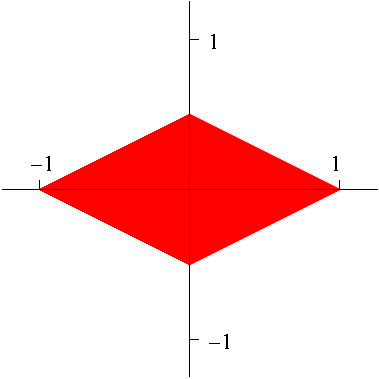
\includegraphics[width=0.3\textwidth]{fcv/number/diamond-112}
      \end{center}
      \caption{The solution is a diamond shape.}
      \label{diamond-112}
    \end{figure}
  \item
    $|z - \imath|$ is the distance from the point $\imath$ in the complex plane.
    Thus $1 < |z - \imath| < 2$ is an annulus centered at $z = \imath$ between the
    radii $1$ and $2$.  See Figure~\ref{annulus-i12}.
    \begin{figure}[h!]
      \begin{center}
        \includegraphics[width=0.25\textwidth]{fcv/number/annulus-i12}
      \end{center}
      \caption{The annulus.}
      \label{annulus-i12}
    \end{figure}
  \item
    The points which are closer to $z = \imath$ than $z = - \imath$ are those points in 
    the upper half plane.  See Figure~\ref{upper-half-domain}.
    \begin{figure}[h!]
      \begin{center}
        \includegraphics[width=0.3\textwidth]{fcv/number/upper-half-domain}
      \end{center}
      \caption{The upper half plane.}
      \label{upper-half-domain}
    \end{figure}
  \end{enumerate}
\end{Solution}








%% argument identities
\begin{Solution}
  \label{solution argument identities}
  Let $z = r \e^{\imath \theta}$ and $\zeta = \rho \e^{\imath \phi}$.
  \begin{enumerate}
  \item
    \begin{gather*}
      \arg(z \zeta) = \arg(z) + \arg(\zeta) \\
      \arg\left( r \rho \e^{\imath (\theta + \phi)} \right) = \{ \theta + 2 \pi m \} + \{ \phi + 2 \pi n \} \\
      \{ \theta + \phi + 2 \pi k \} = \{ \theta + \phi + 2 \pi m \} 
    \end{gather*}
  \item
    \[
    \Arg(z \zeta) \neq \Arg(z) + \Arg(\zeta)
    \]
    Consider $z = \zeta = -1$.  $\Arg(z) = \Arg(\zeta) = \pi$, however 
    $\Arg(z \zeta) = \Arg(1) = 0$.  The identity becomes $0 \neq 2 \pi$.
  \item
    \begin{gather*}
      \arg\left( z^2 \right) = \arg(z) + \arg(z) \neq 2 \arg(z) 
      \\
      \arg\left( r^2 \e^{\imath 2 \theta} \right) 
      = \{ \theta + 2 \pi k \} + \{ \theta + 2 \pi m \} \neq 2 \{ \theta + 2 \pi n \} 
      \\
      \{ 2 \theta + 2 \pi k \} = \{ 2 \theta + 2 \pi m \} \neq \{ 2 \theta + 4 \pi n \} 
    \end{gather*}
  \end{enumerate}
\end{Solution}





%% triangle inequalities
\begin{Solution}
  \label{solution triangle inequalities}
  Consider a triangle in the complex plane with vertices at $0$, $z$
  and $z + \zeta$.  (See Figure~\ref{triangle}.)
  \begin{figure}[h!]
    \begin{center}
      \includegraphics[width=0.3\textwidth]{fcv/number/triangle}
    \end{center}
    \caption{Triangle inequality.}
    \label{triangle}
  \end{figure}

  The lengths of the sides of the triangle are $|z|$, $|\zeta|$ and 
  $|z + \zeta|$  The second inequality shows that one side of the triangle must 
  be less than or equal to the sum of the other two sides.  
  \[
  |z + \zeta| \leq |z| + |\zeta|
  \]
  The first inequality
  shows that the length of one side of the triangle must be greater than
  or equal to the difference in the length of the other two sides.
  \[
  |z + \zeta| \geq ||z| - |\zeta||
  \]

  Now we prove the inequalities algebraically.  We will reduce the inequality
  to an identity.  Let $z = r \e^{\imath \theta}$, $\zeta = \rho \e^{\imath \phi}$.
  \begin{gather*}
    ||z| - |\zeta||\leq |z + \zeta| \leq |z| + |\zeta| 
    \\
    |r - \rho| \leq |r \e^{\imath \theta} + \rho \e^{\imath \phi}| \leq r + \rho 
    \\
    \left( r - \rho \right)^2 \leq \left( r \e^{\imath \theta} + \rho \e^{\imath \phi} \right)
    \left( r \e^{- \imath \theta} + \rho \e^{- \imath \phi} \right) 
    \leq \left( r + \rho \right)^2 
    \\
    r^2 + \rho^2 - 2 r \rho \leq r^2 + \rho^2 + r \rho \e^{\imath \left( \theta - \phi \right)} +
    r \rho \e^{\imath \left( - \theta + \phi \right)} \leq r^2 + \rho^2 + 2 r \rho 
    \\
    - 2 r \rho \leq 2 r \rho \cos\left( \theta - \phi \right) \leq 2 r \rho 
    \\
    -1 \leq \cos(\theta - \phi) \leq 1
  \end{gather*}
\end{Solution}






%% $(-1)^{-3/4}$ $8^{1/6}$
\begin{Solution}
  \label{solution -1 -3/4 8 1/6}
  \begin{enumerate}
    %%
  \item
    \begin{align*}
      (- 1)^{-3/4} 
      &= \left( (- 1)^{-3} \right)^{1/4} 
      \\
      &= (- 1)^{1/4} 
      \\
      &= \left( \e^{\imath \pi} \right)^{1/4} 
      \\
      &= \e^{\imath \pi / 4} 1^{1/4} 
      \\
      &= \e^{\imath \pi / 4} \e^{\imath k \pi / 2}, \quad k = 0,1,2,3 
      \\
      &= \left\{ \e^{\imath \pi / 4}, \e^{\imath 3 \pi / 4}, \e^{\imath 5 \pi / 4}, \e^{\imath 7 \pi / 4} \right\} 
      \\
      &= \left\{ \frac{1 + \imath}{\sqrt{2}}, \frac{- 1 + \imath}{\sqrt{2}},
        \frac{-1 - \imath}{\sqrt{2}}, \frac{1 - \imath}{\sqrt{2}} \right\}
    \end{align*}
    See Figure~\ref{roots_1_3_4}.

    \begin{figure}[h!]
      \begin{center}
        \includegraphics[width=0.3\textwidth]{fcv/number/roots_1_3_4}
      \end{center}
      \caption{The four roots.}
      \label{roots_1_3_4}
    \end{figure}
    %%
  \item
    \begin{align*}
      8^{1/6}
      &= \sqrt[6]{8} 1^{1/6} 
      \\
      &= \sqrt{2} \e^{\imath k \pi / 3}, \quad k = 0,1,2,3,4,5 
      \\
      &= \left\{ \sqrt{2}, 
        \sqrt{2} \e^{\imath \pi / 3},
        \sqrt{2} \e^{\imath 2 \pi / 3},
        \sqrt{2} \e^{\imath \pi},
        \sqrt{2} \e^{\imath 4 \pi / 3},
        \sqrt{2} \e^{\imath 5 \pi / 3} \right\} 
      \\
      &= \left\{ \sqrt{2},
        \frac{1 + \imath \sqrt{3}}{\sqrt{2}},
        \frac{-1 + \imath \sqrt{3}}{\sqrt{2}},
        - \sqrt{2},
        \frac{-1 - \imath \sqrt{3}}{\sqrt{2}},
        \frac{1 - \imath \sqrt{3}}{\sqrt{2}} \right\}
    \end{align*}
    See Figure~\ref{roots_8_1_6}.

    \begin{figure}[h!]
      \begin{center}
        \includegraphics[width=0.3\textwidth]{fcv/number/roots_8_1_6}
      \end{center}
      \caption{The six roots.}
      \label{roots_8_1_6}
    \end{figure}

  \end{enumerate}
\end{Solution}












%% (-1)^{-1/4}
\begin{Solution}
  \label{solution 16 1/8}
  \begin{enumerate}
  \item
    \begin{align*}
      (-1)^{-1/4}
      &= ((-1)^{-1})^{1/4} 
      \\
      &= (-1)^{1/4} 
      \\
      &= \left( \e^{\imath \pi} \right)^{1/4} 
      \\
      &= \e^{\imath \pi / 4} 1^{1/4} 
      \\
      &= \e^{\imath \pi / 4} \e^{\imath k \pi / 2}, \quad k = 0, 1, 2, 3 
      \\
      &= \left\{ \e^{\imath \pi / 4}, \e^{\imath 3 \pi / 4}, \e^{\imath 5 \pi / 4}, \e^{\imath 7 \pi / 4} \right\} 
      \\
      &= \left\{ \frac{1 + \imath}{\sqrt{2}}, \frac{-1 + \imath}{\sqrt{2}},
        \frac{-1 - \imath}{\sqrt{2}}, \frac{1 - \imath}{\sqrt{2}} \right\}
    \end{align*}
    See Figure~\ref{roots_1_1_4}.

    \begin{figure}[h!]
      \begin{center}
        \includegraphics[width=0.3\textwidth]{fcv/number/roots_1_1_4}
      \end{center}
      \caption{The four roots.}
      \label{roots_1_1_4}
    \end{figure}
    %%
  \item
    \begin{align*}
      16^{1/8}
      &= \sqrt[8]{16}  1^{1/8} 
      \\
      &= \sqrt{2} \e^{\imath k \pi / 4}, \quad k = 0,1,2,3,4,5,6,7 
      \\
      &= \left\{ \sqrt{2}, 
        \sqrt{2} \e^{\imath \pi / 4}, 
        \sqrt{2} \e^{\imath \pi / 2}, 
        \sqrt{2} \e^{\imath 3 \pi / 4}, 
        \sqrt{2} \e^{\imath \pi}, 
        \sqrt{2} \e^{\imath 5 \pi / 4}, 
        \sqrt{2} \e^{\imath 3 \pi / 2}, 
        \sqrt{2} \e^{\imath 7 \pi / 4} \right\} 
      \\
      &= \left\{ \sqrt{2}, 
        1 + \imath, 
        \imath \sqrt{2}, 
        - 1 + \imath, 
        - \sqrt{2},
        -1 - \imath, 
        - \imath \sqrt{2}, 
        1 - \imath \right\} 
    \end{align*}
    See Figure~\ref{roots_16_1_8}.

    \begin{figure}[h!]
      \begin{center}
        \includegraphics[width=0.3\textwidth]{fcv/number/roots_16_1_8}
      \end{center}
      \caption{The eight roots.}
      \label{roots_16_1_8}
    \end{figure}
  \end{enumerate}
\end{Solution}












%% $1 < |z - 2 \imath| < 2$ $| \Re(z) | + 5 | \Im(z) | = 1$
\begin{Solution}
  \label{solution 1 z-i2 2}
  \begin{enumerate}
    %%
  \item
    $|z - \imath 2|$ is the distance from the point $\imath 2$ in the complex plane.
    Thus $1 < |z - \imath 2| < 2$ is an annulus.  See Figure~\ref{annulus_1_2i}.

    \begin{figure}[h!]
      \begin{center}
        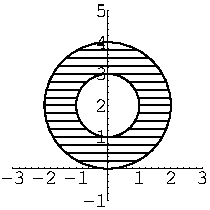
\includegraphics[width=0.25\textwidth]{fcv/number/annulus_1_2i}
      \end{center}
      \caption{The annulus.}
      \label{annulus_1_2i}
    \end{figure}
    %%
  \item
    \begin{gather*}
      | \Re(z) | + 5 | \Im(z) | = 1 \\
      | x | + 5 | y | = 1 
    \end{gather*}
    In the first quadrant this is the line $y = (1 - x) / 5$.  We reflect this
    line segment across the coordinate axes to obtain line segments in the 
    other quadrants.  Explicitly, we have the set of points: 
    $\{z = x + \imath y \mid -1 < x < 1 \land y = \pm (1 - |x|) / 5 \}$.
    See Figure~\ref{diamond}.

    \begin{figure}[h!]
      \begin{center}
        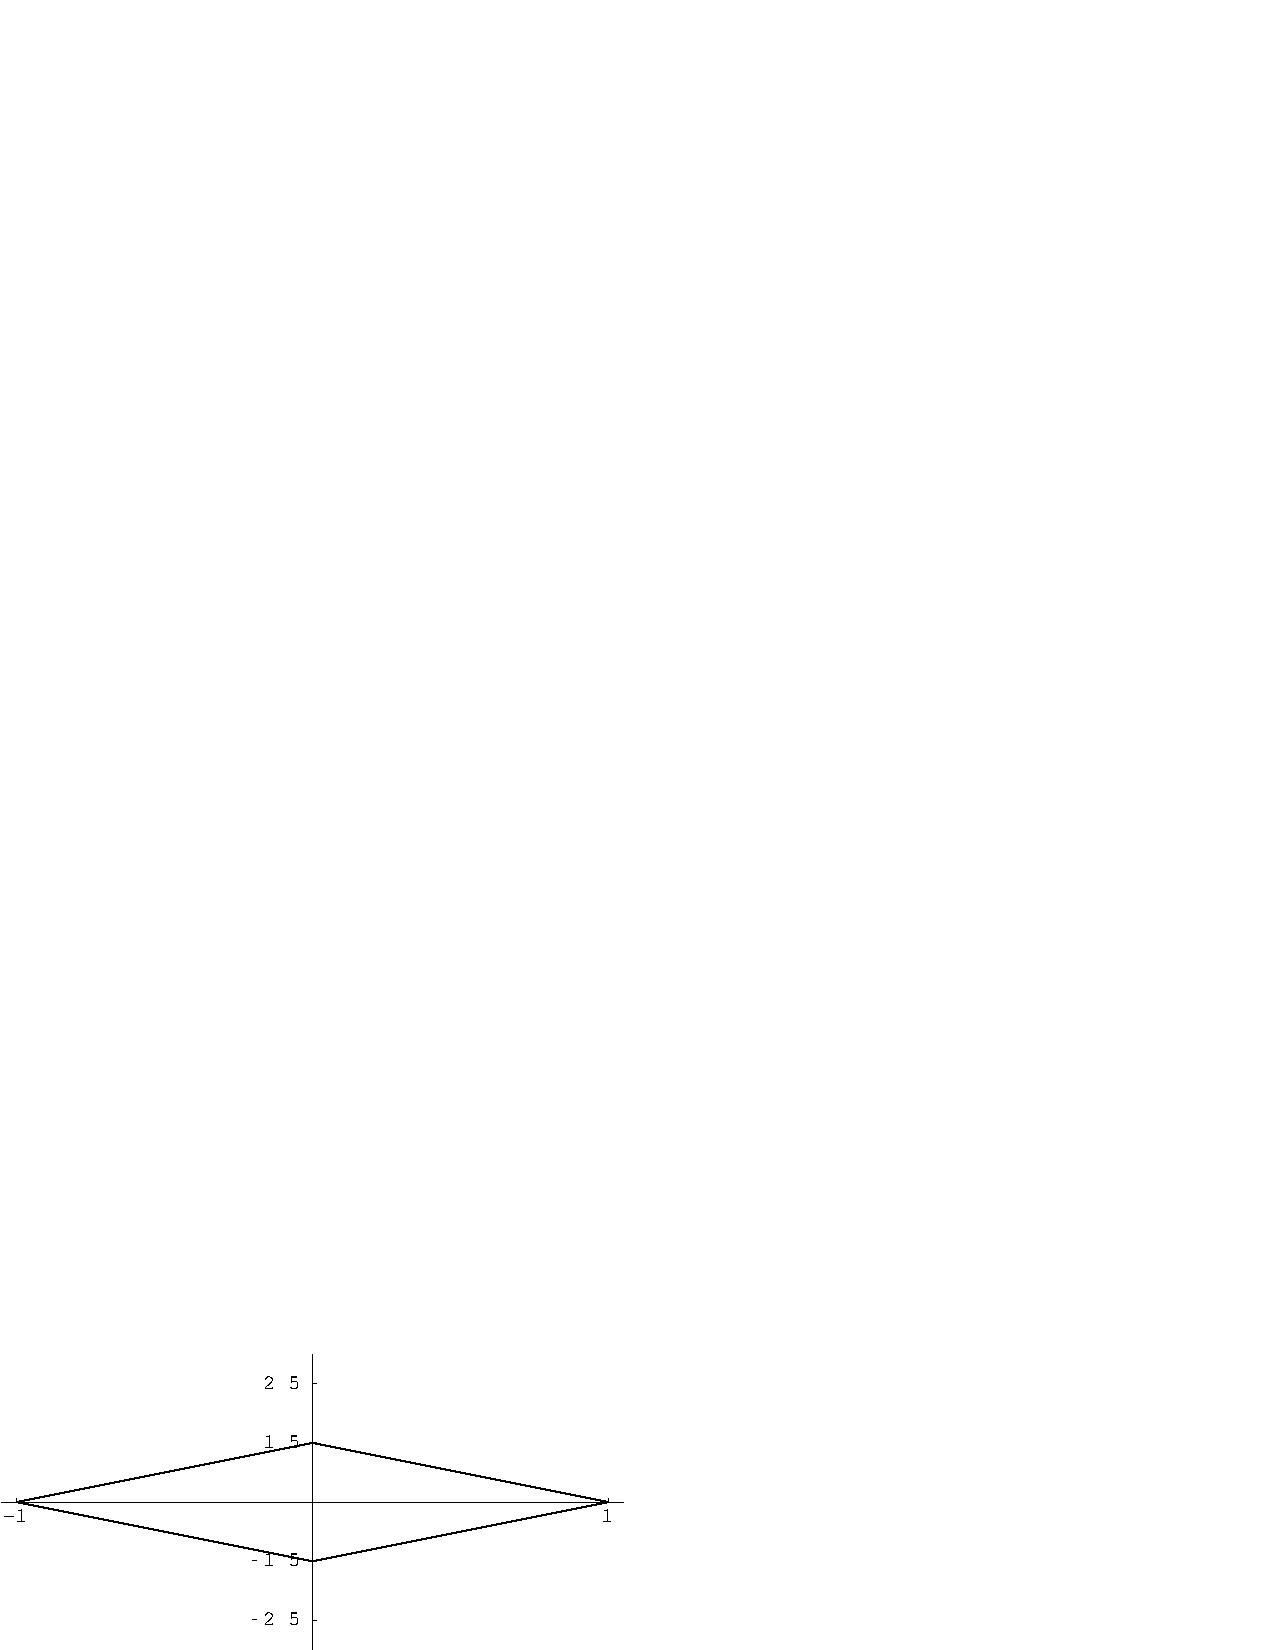
\includegraphics[width=0.5\textwidth]{fcv/number/diamond}
      \end{center}
      \caption{The solution is a diamond shape.}
      \label{diamond}
    \end{figure}
    %%
  \item
    The set of points equidistant from $\imath$ and $-\imath$ is the real axis.
    See Figure~\ref{real_axis}.
    \begin{figure}[h!]
      \begin{center}
        \includegraphics[width=0.4\textwidth]{fcv/number/real_axis}
      \end{center}
      \caption{The solution is the real axis.}
      \label{real_axis}
    \end{figure}
  \end{enumerate}
\end{Solution}















%% |z - 1 + \imath|\leq 1
\begin{Solution}
  \label{solution z-1+i 1}
  \begin{enumerate}
  \item
    $|z - 1 + \imath|$ is the distance from the point $(1 - \imath)$.  Thus 
    $|z - 1 + \imath| \leq 1$ is
    the disk of unit radius centered at $(1 - \imath)$.
    See Figure~\ref{disk_1_mi}.
    \begin{figure}[h!]
      \begin{center}
        \includegraphics[width=0.3\textwidth]{fcv/number/disk_1_mi}
      \end{center}
      \caption{A disk of unit raduis.}
      \label{disk_1_mi}
    \end{figure}
    %%
  \item
    \begin{gather*}
      \Re(z)- \Im(z) = 5 
      \\
      x - y = 5 
      \\
      y = x - 5
    \end{gather*}
    See Figure~\ref{line_yx5}.
    \begin{figure}[h!]
      \begin{center}
        \includegraphics[width=0.5\textwidth]{fcv/number/line_yx5}
      \end{center}
      \caption{The solution is a line.}
      \label{line_yx5}
    \end{figure}
    %%
    %%
    %%
  \item
    Since $|z - \imath| + |z + \imath| \geq 2$, there are no solutions of 
    $|z - \imath| + |z + \imath| = 1$.
  \end{enumerate}
\end{Solution}









%% |\e^{\imath \theta}-1| =2
\begin{Solution}
  \label{solution e i theta - 1 = 2}
  \begin{gather*}
    |\e^{\imath \theta} - 1| = 2 
    \\
    \left( \e^{\imath \theta} - 1 \right) \left( \e^{-\imath \theta} - 1 \right) = 4 
    \\
    1 - \e^{\imath \theta} - \e^{-\imath \theta} + 1 = 4 
    \\
    -2 \cos(\theta) = 2 
    \\
    \theta = \pi
  \end{gather*}

  $\left\{ \e^{\imath \theta} \mid 0 \leq \theta \leq \pi \right\}$ is a unit semi-circle in the
  upper half of the complex plane from $1$ to $-1$.  The only point on this
  semi-circle that is a distance $2$ from the point $1$ is the point $-1$,
  which corresponds to $\theta = \pi$.
\end{Solution}









%%-----------------------------------------------------------------------------
\begin{large}
  \noindent
  \textbf{Polar Form}
\end{large}




%% Euler's formula
\begin{Solution}
  \label{solution eulers formula}
  We recall the Taylor series expansion of $\e^x$ about $x = 0$.
  \[
  \e^x = \sum_{n = 0}^\infty \frac{x^n}{n!}.
  \]
  We take this as the definition of the exponential function for complex
  argument.
  \begin{align*}
    \e^{\imath \theta} 
    &= \sum_{n = 0}^\infty \frac{(\imath \theta)^n}{n!} 
    \\
    &= \sum_{n = 0}^\infty \frac{\imath^n}{n!} \theta^n
    \\
    &= \sum_{n = 0}^\infty \frac{(-1)^n}{(2 n)!} \theta^{2n}
    + \imath \sum_{n = 0}^\infty \frac{(-1)^n}{(2 n + 1)!} \theta^{2n+1}
  \end{align*}
  We compare this expression to the Taylor series for the sine and cosine.
  \[
  \cos \theta = \sum_{n = 0}^\infty \frac{(-1)^n}{(2 n)!} \theta^{2n}, \qquad
  \sin \theta = \sum_{n = 0}^\infty \frac{(-1)^n}{(2 n + 1)!} \theta^{2n+1}, \qquad
  \]
  Thus $\e^{\imath \theta}$ and $\cos \theta + \imath \sin \theta$ have the same Taylor
  series expansions about $\theta = 0$. 
  \[
  \boxed{
    \e^{\imath \theta} = \cos \theta + \imath \sin \theta
    }
  \]
\end{Solution}








%% \cos(3\theta) = \cos^3(\theta) -3\cos(\theta)\sin^2(\theta).
\begin{Solution}
  \label{solution cos 3t = cos3 t - 3 cos t sin2 t}
  \begin{gather*}
    \cos(3 \theta) + \imath \sin(3 \theta) = (\cos \theta + \imath \sin \theta)^3 
    \\
    \cos(3 \theta) + \imath \sin(3 \theta) = \cos^3 \theta + \imath 3 \cos^2 \theta \sin \theta
    - 3 \cos \theta \sin^2 \theta - \imath \sin^3 \theta 
    \\
    \intertext{We equate the real parts of the equation.}
    \cos(3 \theta) = \cos^3 \theta - 3 \cos \theta \sin^2 \theta 
  \end{gather*}
\end{Solution}








%% 1 + z + z^2 + \cdots + z^n = \frac{1 - z^{n+1}}{1-z}, \qquad (z \neq 1),
\begin{Solution}
  \label{solution geometric trig identity}
  Define the partial sum,
  \[
  S_n(z) = \sum_{k=0}^n z^k.
  \]
  Now consider $(1 - z) S_n(z)$.
  \begin{gather*}
    (1 - z) S_n(z) = (1 - z) \sum_{k=0}^n z^k 
    \\
    (1 - z) S_n(z) = \sum_{k=0}^n z^k - \sum_{k=1}^{n+1} z^k 
    \\
    (1 - z) S_n(z) = 1 - z^{n+1} 
    \\
    \intertext{We divide by $1 - z$.  Note that $1 - z$ is nonzero.}
    S_n(z) = \frac{1 - z^{n+1} }{ 1 - z } 
    \\
    1 + z + z^2 + \cdots + z^n = \frac{1 - z^{n+1}}{1 - z}, \qquad (z \neq 1)
  \end{gather*}

  Now consider $z = \e^{\imath \theta}$ where $0 < \theta < 2 \pi$ so that $z$ is not unity.
  \begin{gather*}
    \sum_{k = 0}^n \left( \e^{\imath \theta} \right)^k = \frac{1 - \left( \e^{\imath \theta} \right)^{n+1} }{1 - \e^{\imath \theta}}
    \\
    \sum_{k = 0}^n \e^{\imath k \theta} = \frac{1 - \e^{\imath (n+1) \theta} }{1 - \e^{\imath \theta}} 
    \\
    \intertext{In order to get $\sin(\theta/2)$ in the denominator, we 
      multiply top and bottom by $\e^{-\imath \theta / 2}$.}
    \sum_{k = 0}^n (\cos(k \theta) + \imath \sin(k \theta) ) =
    \frac{\e^{- \imath \theta / 2} - \e^{\imath (n+1/2) \theta} }{\e^{-\imath \theta / 2} - \e^{\imath \theta / 2}} 
    \\
    \sum_{k = 0}^n \cos(k \theta) + \imath \sum_{k = 0}^n \sin(k \theta) =
    \frac{ \cos(\theta/2) - \imath \sin(\theta/2)
      - \cos((n+1/2) \theta) - \imath \sin((n+1/2) \theta) }{ - 2 \imath \sin(\theta/2) } 
    \\
    \sum_{k = 0}^n \cos(k \theta) + \imath \sum_{k = 1}^n \sin(k \theta) =
    \frac{1}{2} + \frac{ \sin((n+1/2) \theta) }{ \sin(\theta/2) }
    + \imath \left( \frac{1}{2} \cot(\theta/2)
      - \frac{ \cos((n+1/2) \theta) }{ \sin(\theta/2) } \right)
  \end{gather*}


  \begin{enumerate}
    %%
  \item
    We take the real and imaginary part of this to obtain the identities.
    \[
    \boxed{
      \sum_{k = 0}^n \cos(k \theta) =
      \frac{1}{2} + \frac{ \sin((n + 1/2) \theta) }
      { 2 \sin(\theta/2) }
      }
    \]
    %%
  \item
    \[
    \boxed{
      \sum_{k = 1}^n \sin(k \theta) =
      \frac{1}{2} \cot(\theta/2) 
      - \frac{ \cos((n+1/2) \theta ) }{ 2 \sin(\theta/2) }
      }
    \]
  \end{enumerate}
\end{Solution}







%%-----------------------------------------------------------------------------
\begin{large}
  \noindent
  \textbf{Arithmetic and Vectors}
\end{large}







%% modulus identities with polar form
\begin{Solution}
  \label{solution modulus identities polar}
  \begin{align*}
    |z \zeta| &= |r \e^{\imath \theta} \rho \e^{\imath \phi} | 
    \\
    &= | r \rho \e^{\imath \left( \theta + \phi \right)} | 
    \\
    &= |r \rho| 
    \\
    &= |r| |\rho| 
    \\
    &= |z| |\zeta|
  \end{align*}
  \begin{align*}
    \left| \frac{z}{\zeta} \right|
    &= \left| \frac{r \e^{\imath \theta}}{\rho \e^{\imath \phi}} \right| 
    \\
    &= \left| \frac{r}{\rho} \e^{\imath \left( \theta - \phi \right)} \right| 
    \\
    &= \left| \frac{r}{\rho} \right| 
    \\
    &= \frac{|r|}{|\rho|} 
    \\
    &= \frac{|z|}{|\zeta|}
  \end{align*}
\end{Solution}









%% parallelogram identity
\begin{Solution}
  \label{solution parallelogram identity}
  \begin{align*}
    \left| z + \zeta \right|^2 + \left| z - \zeta \right|^2
    &= \left( z + \zeta \right) \left( \overline{z} + \overline{\zeta} \right)
    + \left( z - \zeta \right) \left( \overline{z} - \overline{\zeta} \right) 
    \\
    &= z \overline{z} + z \overline{\zeta} + \zeta \overline{z} + \zeta \overline{\zeta}
    + z \overline{z} - z \overline{\zeta} - \zeta \overline{z} + \zeta \overline{\zeta} 
    \\
    &= 2 \left( \left| z \right|^2 + \left| \zeta \right|^2 \right)
  \end{align*}
  Consider the parallelogram defined by the vectors $z$ and $\zeta$.  
  The lengths of the sides are $z$ and $\zeta$ and the lengths of the 
  diagonals are $z + \zeta$ and $z - \zeta$.  
  We know from geometry that the sum of the squared lengths of the diagonals
  of a parallelogram is equal to the sum of the squared lengths of the four
  sides.  (See Figure~\ref{para_identity}.)
  \begin{figure}[h!]
    \begin{center}
      \includegraphics[width=0.15\textwidth]{fcv/number/para_identity}
    \end{center}
    \caption{The parallelogram.}
    \label{para_identity}
  \end{figure}
\end{Solution}



%%-----------------------------------------------------------------------------
\begin{large}
  \noindent
  \textbf{Integer Exponents}
\end{large}



%% (1 + \imath)^{10}
\begin{Solution}
  \label{solution (1+i)10}
  \begin{enumerate}
  \item
    \begin{align*}
      (1 + \imath)^{10}
      &= \left( \left( (1 + \imath)^2 \right)^2 \right)^2 (1 + \imath)^2 
      \\
      &= \left( \left( \imath 2 \right)^2 \right)^2 (\imath 2) 
      \\
      &= \left( -4 \right)^2 (\imath 2) 
      \\
      &= 16 (\imath 2) 
      \\
      &= \imath 32
    \end{align*}
  \item
    \begin{align*}
      (1 + \imath)^{10}
      &= \left( \sqrt{2} \e^{\imath \pi/4} \right)^{10} 
      \\
      &= \left( \sqrt{2} \right)^{10} \e^{\imath 10 \pi/4} 
      \\
      &= 32 \e^{\imath \pi/2} 
      \\
      &= \imath 32
    \end{align*}
  \end{enumerate}
\end{Solution}




%%-----------------------------------------------------------------------------
\begin{large}
  \noindent
  \textbf{Rational Exponents}
\end{large}



%% Quadratic formula
\begin{Solution}
  \label{solution z2 + 2az + b = 0}
  We substitite the numbers into the equation to obtain an identity.
  \begin{gather*}
    z^2 + 2 a z + b = 0 
    \\
    \left( -a + \left( a^2 - b \right)^{1/2} \right)^2 
    + 2 a \left( -a + \left( a^2 - b \right)^{1/2} \right) + b = 0 
    \\
    a^2 -2 a \left( a^2 - b \right)^{1/2} + a^2 - b - 2 a^2 
    + 2 a \left( a^2 - b \right)^{1/2} + b = 0 
    \\
    0 = 0
  \end{gather*}
\end{Solution}









\raggedbottom

}


%%-----------------------------------------------------------------------------
%%
%%                                   Sean Mauch
%%                       California Institute of Technology
%%                         @ 1995-2004 No Rights Reserved
%%
%%-----------------------------------------------------------------------------

\flushbottom


%% CONTINUE:
%% This may be a good chapter to introduce mappings.
%% CONTINUE:
%% Perhaps cover singularities before branch points.




%%============================================================================
%%============================================================================
\chapter{Functions of a Complex Variable}


If brute force isn't working, you'{}re not using enough of it.

\begin{flushright}
  -Tim Mauch
\end{flushright}






In this chapter we introduce the algebra of functions of a complex
variable.  We will cover the trigonometric and inverse trigonometric 
functions.  The properties of trigonometric functions carry over 
directly from real-variable theory.  However, because of multi-valuedness,
the inverse trigonometric functions are significantly trickier than
their real-variable counterparts.









%%=============================================================================
\section{Curves and Regions}


In this section we introduce curves and regions in the complex plane.  This 
material is necessary for the study of branch points in this chapter and
later for contour integration.


\paragraph{Curves.}
Consider two continuous functions $x(t)$ and $y(t)$ defined on the
interval $t \in [t_0 .. t_1]$.  The set of points in the complex plane,
\[
\{ z(t) = x(t) + \imath y(t) \mid t \in [t_0 \ldots t_1] \},
\]
defines a \textit{continuous curve} or simply a \textit{curve}.
\index{curve}
\index{curve!continuous}
If the endpoints coincide ( $z \left( t_0 \right) = z \left( t_1 \right)$ )
it is a \textit{closed curve}.
\index{curve!closed}
(We assume that $t_0 \neq t_1$.)
If the curve does not intersect itself, then it is said to be a
\textit{simple curve}.
\index{curve!simple}

If $x(t)$ and $y(t)$ have continuous derivatives and the derivatives
do not both vanish at any point, then it is a \textit{smooth curve}.%
\footnote{Why is it necessary that the derivatives do not both vanish?}
%% CONTINUE add an exercise concerning vanishing derivatives and corners.
\index{curve!smooth}
This essentially means that the curve does not have any corners or other
nastiness.

A continuous curve which is composed of a finite number of smooth curves
is called a \textit{piecewise smooth curve}.
\index{curve!piecewise smooth}
We will use the word \textit{contour}
\index{contour}
as a synonym for a piecewise smooth curve.


See Figure~\ref{curves} for a smooth curve, a piecewise smooth curve,
a simple closed curve and a non-simple closed curve.
\begin{figure}[htbp!]
  \begin{center}
      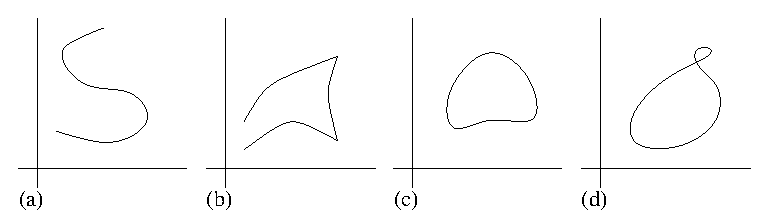
\includegraphics[width=0.8\textwidth]{fcv/function/curves}
  \end{center}
  \caption{(a) Smooth curve. (b) Piecewise smooth curve.
    (c) Simple closed curve. (d) Non-simple closed curve.}
  \label{curves}
\end{figure}






\paragraph{Regions.}
A region $R$ is \textit{connected} if any two points in $R$ can be connected
\index{connected region}
\index{region!connected}
by a curve which lies entirely in $R$.
A region is \textit{simply-connected} if every closed curve
\index{region!simply-connected}
in $R$ can be continuously shrunk to a point without leaving $R$.
A region which is not simply-connected is said to be
\textit{multiply-connected region}.
\index{region!multiply-connected}
Another way of defining simply-connected is that a path connecting two
points in $R$ can be continuously deformed into any other path that connects
those points.  Figure~\ref{regions} shows a simply-connected region with
two paths which can be continuously deformed into one another and two
multiply-connected regions with paths which cannot be deformed into one
another.

\begin{figure}[htb!]
  \begin{center}
      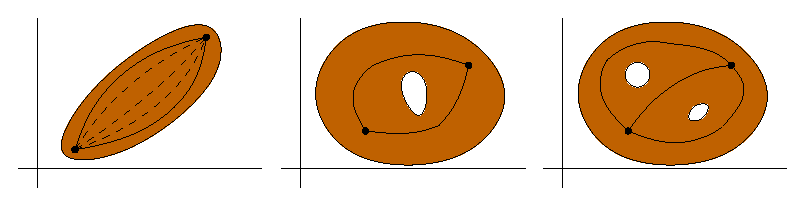
\includegraphics[width=0.9\textwidth]{fcv/function/regions}
  \end{center}
  \caption{A simply-connected and two multiply-connected regions.}
  \label{regions}
\end{figure}





\paragraph{Jordan curve theorem.}
A continuous, simple, closed curve is known as a \textit{Jordan curve}.
\index{curve!Jordan}
\index{Jordan curve}
The Jordan Curve Theorem, which seems intuitively obvious but is difficult
to prove, states that a Jordan curve divides the plane into a simply-connected,
bounded region and an unbounded region.  These two regions are called the
interior and exterior regions, respectively.  The two regions share the
curve as a boundary.  Points in the interior are said to be inside
the curve; points in the exterior are said to be outside the curve.







\paragraph{Traversal of a contour.}
\index{contour!traversal of}
Consider a Jordan curve.  If you traverse the curve in the
\textit{positive} direction, then the inside is to your left.  If you traverse%
\index{direction!positive}
\index{direction!negative}
\index{clockwise}
\index{counter-clockwise}
the curve in the opposite direction, then the outside will be to your
left and you will go around the curve in the negative direction.
For circles, the positive direction is the
\textit{counter-clockwise} direction.   The positive direction is
consistent with the way angles are measured in a right-handed coordinate
system,  i.e. for a circle centered on the origin, the positive direction
is the direction of increasing angle.  For an oriented contour $C$,
we denote the contour with opposite orientation as $-C$.



\paragraph{Boundary of a region.}
Consider a simply-connected region.  The boundary of the region is
traversed in the positive direction if the region is to the left as you
walk along the contour.  For multiply-connected regions, the boundary
may be a set of contours.  In this case the boundary is traversed in the
positive direction if each of the contours is traversed in the positive
direction.  When we refer to the boundary of a region we will assume it
is given the positive orientation.
In Figure~\ref{pos_boundary} the boundaries of three regions
are traversed in the positive direction.

\begin{figure}[htb!]
  \begin{center}
    
\includegraphics[width=0.6\textwidth]{fcv/function/pos_boundary}
  \end{center}
  \caption{Traversing the boundary in the positive direction.}
  \label{pos_boundary}
\end{figure}




\paragraph{Two interpretations of a curve.}
Consider a simple closed curve as depicted in Figure~\ref{two_views}a.
By giving it an orientation, we can make a contour that either
encloses the bounded domain Figure~\ref{two_views}b or the unbounded
domain Figure~\ref{two_views}c.  Thus a curve has two interpretations.
It can be thought of as enclosing either the points which are
``inside'' or the points which are ``outside''.%
\footnote{
  A farmer wanted to know the most efficient way to build a pen to
  enclose his sheep, so he consulted an engineer, a physicist and a
  mathematician.  The engineer suggested that he build a circular pen
  to get the maximum area for any given perimeter.  The physicist
  suggested that he build a fence at infinity and then shrink it to
  fit the sheep.  The mathematician constructed a little fence around
  himself and then defined himself to be outside.
  }


\begin{figure}[htb!]
  \begin{center}
      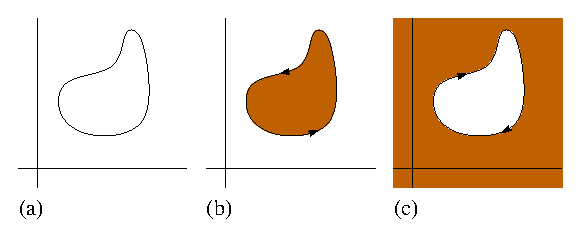
\includegraphics[width=0.6\textwidth]{fcv/function/two_views}
  \end{center}
  \caption{Two interpretations of a curve.}
  \label{two_views}
\end{figure}










%%=============================================================================
\section{The Point at Infinity and the Stereographic Projection}



\paragraph{Complex infinity.}
\index{complex infinity}
\index{infinity!complex}
\index{point at infinity}
\index{infinity!point at}
\index{extended complex plane}
In real variables, there are only two ways to get to infinity.  
We can either go up or down the number line.  Thus signed infinity makes 
sense.  By going up or down we respectively approach $+ \infty$ and $- \infty$.
In the complex plane there are an infinite number of ways to approach 
infinity.  We stand at the origin, point ourselves in any direction and 
go straight.  We could walk along the positive real axis and approach
infinity via positive real numbers.  We could walk along the positive 
imaginary axis and approach infinity via pure imaginary numbers.  We could
generalize the real variable notion of signed infinity to a complex variable
notion of directional infinity, but this will not be useful for our 
purposes.  Instead, we introduce \textit{complex infinity} or
the \textit{point at infinity} as the limit of going infinitely far
along any direction in the complex plane.  The complex plane together with
the point at infinity form the \textit{extended complex plane}.




\paragraph{Stereographic projection.}
\index{stereographic projection}
We can visualize the point at infinity with the 
\textit{stereographic projection}.  We place a unit 
sphere on top of the complex plane so that the south pole of the sphere
is at the origin.  Consider a line passing through the north pole and 
a point $z = x + \imath y$ in the complex plane.  In the stereographic projection,
the point point $z$ is mapped to the point where the line intersects 
the sphere.  (See Figure~\ref{figure stereographic-projection}.)  Each
point $z = x + \imath y$ in the complex plane is mapped to a unique point 
$(X, Y, Z)$ on the sphere.
\[
X = \frac{4 x}{|z|^2 + 4}, \quad
Y = \frac{4 y}{|z|^2 + 4}, \quad
Z = \frac{2 |z|^2}{|z|^2 + 4}
\]
The origin is mapped to the south pole.  The point at infinity, $|z| = \infty$,
is mapped to the north pole.


\begin{figure}[htbp!]
  \begin{center}
      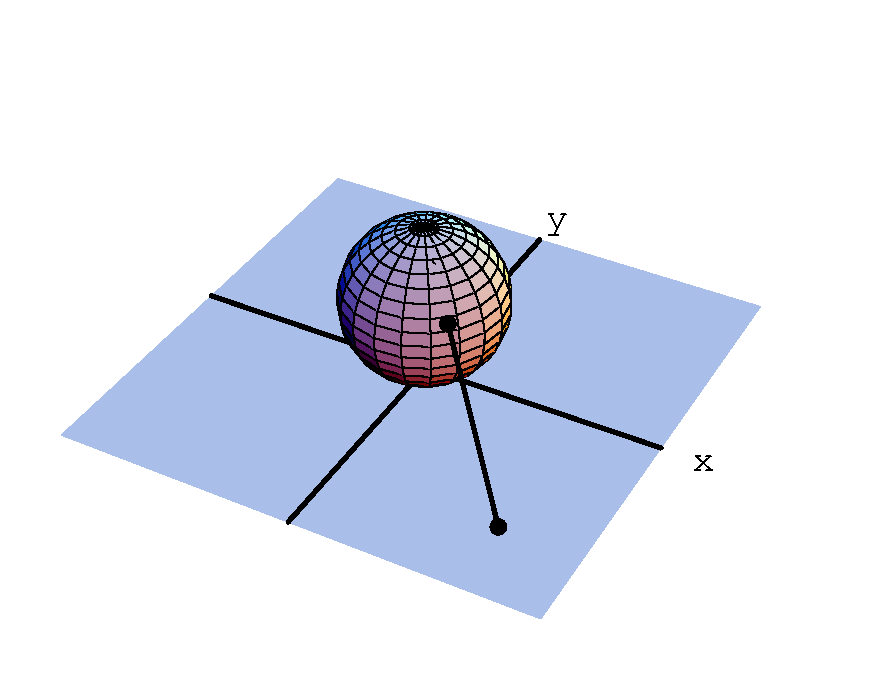
\includegraphics[width=0.5\textwidth]{fcv/function/stereographic-projection}
  \end{center}
  \caption{The stereographic projection.}
  \label{figure stereographic-projection}
\end{figure}



In the stereographic projection, circles in the complex plane are mapped 
to circles on the unit sphere.  Figure~\ref{figure stereo-circle stereo-lines}
shows circles along the real and imaginary axes under the mapping.
Lines in the complex plane are also mapped 
to circles on the unit sphere.  The right diagram in 
Figure~\ref{figure stereo-circle stereo-lines} shows
lines emanating from the origin under the mapping.
\begin{figure}[htbp!]
  \begin{center}
    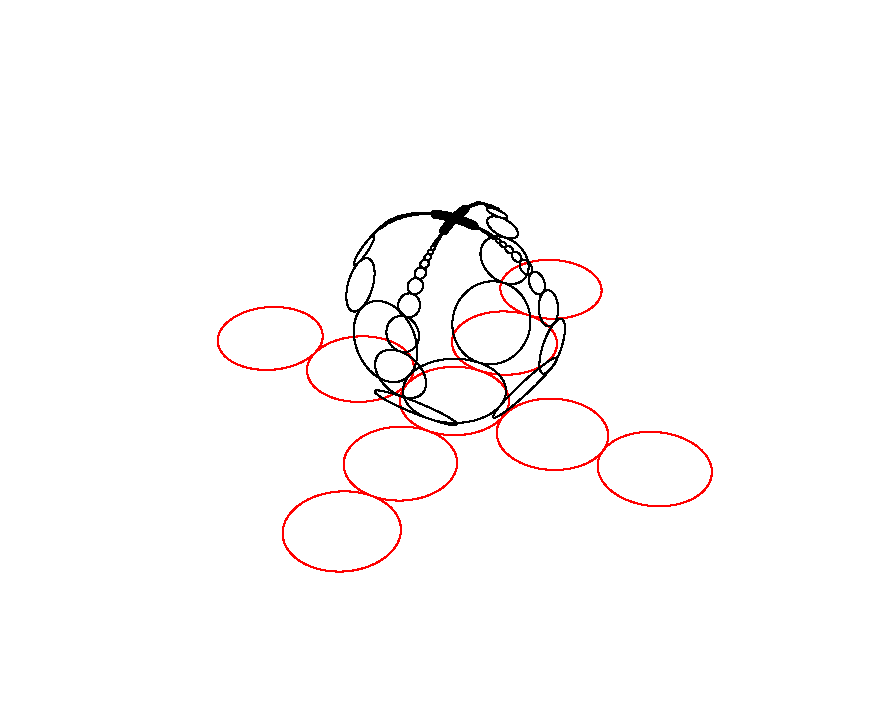
\includegraphics[width=0.49\textwidth]{fcv/function/stereo-circle}
    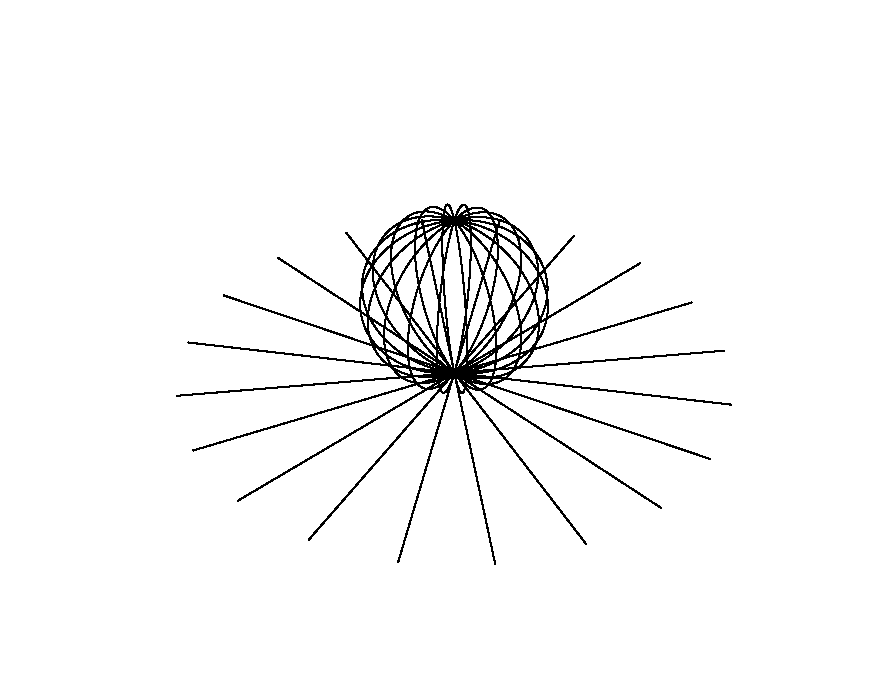
\includegraphics[width=0.49\textwidth]{fcv/function/stereo-line}
  \end{center}
  \caption{The stereographic projection of circles and lines.}
  \label{figure stereo-circle stereo-lines}
\end{figure}


The stereographic projection helps us reason about the point at infinity.
When we consider the complex plane by itself, the point at infinity is an 
abstract notion.  We can't draw a picture of the point at infinity.  It may 
be hard to accept the notion of a jordan curve enclosing the point at 
infinity.  However, in the stereographic projection, the point at infinity
is just an ordinary point (namely the north pole of the sphere).  
%% CONTINUE



%%=============================================================================
\section{A Gentle Introduction to Branch Points}



In this section we will introduce the concepts of \textit{branches}, 
\textit{branch points} and \textit{branch cuts}.  These concepts 
(which are notoriously difficult to understand for beginners)
are typically
defined in terms functions of a complex variable.  Here we will develop
these ideas as they relate to the arctangent function $\arctan(x,y)$.
Hopefully this simple example will make the treatment in 
Section~\ref{chapter function section branch points} more palateable.

First we review some properties of the arctangent.  It is a mapping from
$\mathbb{R}^2$ to $\mathbb{R}$.  It measures the angle around the 
origin from the positive $x$ axis.  Thus it is a multi-valued function.
For a fixed point in the domain, the function values differ by integer 
multiples of $2 \pi$.  The arctangent is not defined at the origin nor 
at the point at infinity; it is singular at these two points.  If we plot 
some of the values of the arctangent, it looks like a corkscrew with 
axis through the origin.  A portion of this function is plotted in
Figure~\ref{arctangent_few}.


\begin{figure}[htbp!]
  \begin{center}
    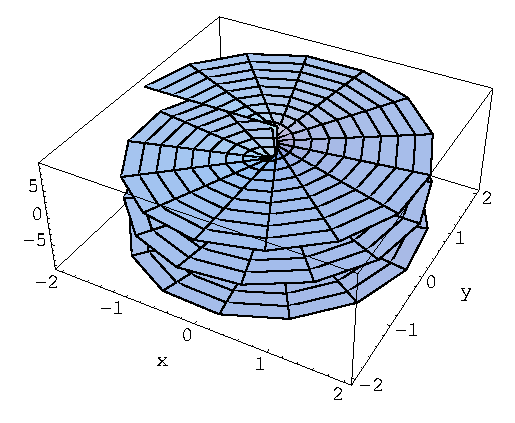
\includegraphics[width=0.4\textwidth]{fcv/function/arctangent_few}
  \end{center}
  \caption{Plots of the real part of the logarithm and a portion of 
    the imaginary part of the logarithm.}
  \label{arctangent_few}
\end{figure}

Most of the tools we have for analyzing functions (continuity, 
differentiability, etc.) depend on the fact that the function is 
single-valued.  In order to work with the arctangent we need to select a 
portion to obtain a single-valued function.  Consider the domain 
$(-1 .. 2) \times (1 .. 4)$.  On this domain we select the value of 
the arctangent that is between $0$ and $\pi$.  The domain and a plot of the 
selected values of the arctangent are shown in 
Figure~\ref{arctangent_square_domain}.

\begin{figure}[htbp!]
  \begin{center}
    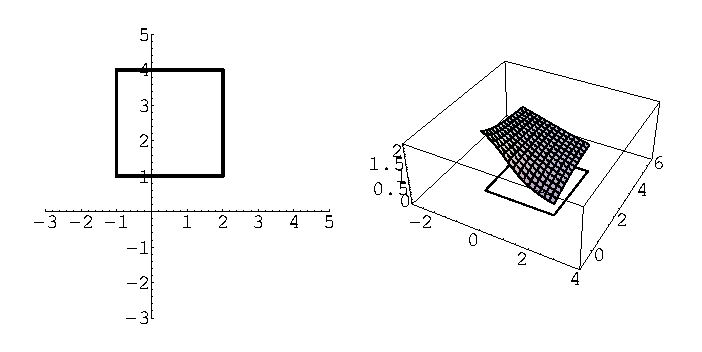
\includegraphics[width=0.7\textwidth]{fcv/function/arctangent_square_domain}
  \end{center}
  \caption{A domain and a selected value of the arctangent for the points
        in the domain.}
  \label{arctangent_square_domain}
\end{figure}




CONTINUE.



%%=============================================================================
\section{Cartesian and Modulus-Argument Form}


We can write a function of a complex variable $z$ as a function of $x$ and $y$
or as a function of $r$ and $\theta$ with the substitutions $z = x + \imath y$
and $z = r \e^{\imath \theta}$, respectively.
Then we can separate the real and imaginary components or write the function
in modulus-argument form,
\[
f(z) = u(x,y) + \imath v(x,y), \quad \mathrm{or} \quad 
f(z) = u(r,\theta) + \imath v(r,\theta),
\]
\[
f(z) = \rho(x,y) \e^{\imath \phi(x,y)}, \quad \mathrm{or} \quad
f(z) = \rho(r,\theta) \e^{\imath \phi(r,\theta)}.
\]



\begin{Example}
  Consider the functions $f(z) = z$, $f(z) = z^3$ and $f(z) = \frac{1}{1-z}$.
  We write the functions in terms of $x$ and $y$ and 
  separate them into their real and imaginary components.
  \begin{align*}
    f(z)    
    &= z 
    \\
    &= x + \imath y
  \end{align*}
  \begin{align*}
    f(z)    
    &= z^3 
    \\
    &= (x + \imath y)^3 
    \\
    &= x^3 + \imath x^2 y - x y^2 - \imath y^3 
    \\
    &= \left( x^3 - x y^2 \right) + \imath \left(x^2 y - y^3 \right)
  \end{align*}
  \begin{align*}
    f(z)    
    &= \frac{1}{1-z} 
    \\
    &= \frac{1}{1 - x - \imath y} 
    \\
    &= \frac{1}{1 - x - \imath y}  \frac{1 - x + \imath y}{1 - x + \imath y} 
    \\
    &= \frac{1-x}{(1-x)^2 + y^2} + \imath \frac{y}{(1-x)^2 + y^2}
  \end{align*}
\end{Example}






\begin{Example}
  Consider the functions $f(z) = z$, $f(z) = z^3$ and $f(z) = \frac{1}{1-z}$.
  We write the functions in terms of $r$ and $\theta$ and 
  write them in modulus-argument form.
  \begin{align*}
    f(z)    
    &= z 
    \\
    &= r \e^{\imath \theta}
  \end{align*}
  \begin{align*}
    f(z)    
    &= z^3 
    \\
    &= \left( r \e^{\imath \theta} \right)^3 
    \\
    &= r^3 \e^{\imath 3 \theta}
  \end{align*}
  \begin{align*}
    f(z)    
    &= \frac{1}{1-z} 
    \\
    &= \frac{1}{1 - r \e^{\imath \theta}} 
    \\
    &= \frac{1}{1 - r \e^{\imath \theta}}  \frac{1}{1 - r \e^{-\imath \theta}} 
    \\
    &= \frac{1 - r \e^{-\imath \theta}}{1 - r \e^{\imath \theta} - r \e^{-\imath \theta} + r^2} 
    \\
    &= \frac{1 - r \cos \theta + \imath r \sin \theta}{1 - 2 r \cos \theta + r^2} 
    \\
    \intertext{Note that the denominator is real and non-negative.}
    &= \frac{1} {1 - 2 r \cos \theta + r^2}  | 1 - r \cos \theta + \imath r \sin \theta | 
    \e^{\imath \arctan(1 - r \cos \theta, r \sin \theta)} 
    \\
    &= \frac{1} {1 - 2 r \cos \theta + r^2}  \sqrt{ (1 - r \cos \theta)^2 + r^2 \sin^2 \theta } 
     \e^{\imath \arctan(1 - r \cos \theta, r \sin \theta)} 
    \\
    &= \frac{1} {1 - 2 r \cos \theta + r^2} 
    \sqrt{ 1 - 2 r \cos \theta + r^2 \cos^2 \theta + r^2 \sin^2 \theta } 
    \e^{\imath \arctan(1 - r \cos \theta, r \sin \theta)} 
    \\
    &= \frac{1}{ \sqrt{ 1 - 2 r \cos \theta + r^2 } }  \e^{\imath \arctan(1 - r \cos \theta, r \sin \theta)} 
  \end{align*}
\end{Example}









%%=============================================================================
\section{Graphing Functions of a Complex Variable}




We cannot directly graph functions of a complex variable as they are 
mappings from $\mathbb{R}^2$ to $\mathbb{R}^2$.  To do so would require four
dimensions.  However, we can can use a surface plot to graph the real part, 
the imaginary part, the modulus or the argument of a function of a complex 
variable.  Each of these are scalar fields, mappings from $\mathbb{R}^2$ to 
$\mathbb{R}$.




\begin{Example}
  Consider the identity function, $f(z) = z$.  In Cartesian coordinates and
  Cartesian form, the function is $f(z) = x + \imath y$.  The real and imaginary
  components are $u(x,y) = x$ and $v(x,y) = y$.  (See Figure~\ref{zreim}.)
  \begin{figure}[htbp!]
    \begin{center}
        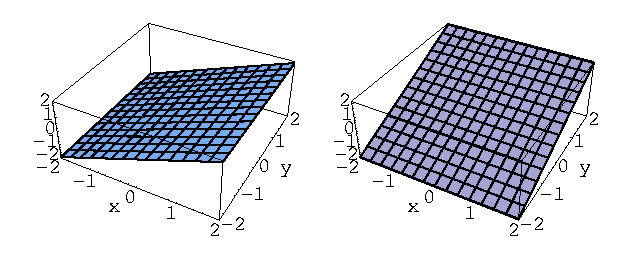
\includegraphics[width=0.6\textwidth]{fcv/function/zreim}
    \end{center}
    \caption{The real and imaginary parts.}
    \label{zreim}
  \end{figure}
  In modulus argument form the function is
  \[
  f(z) = z = r \e^{\imath \theta} = \sqrt{x^2 + y^2}  \e^{\imath \arctan(x,y)}.
  \]
  The modulus of $f(z)$ is a single-valued function which is the distance 
  from the origin.  The argument of $f(z)$ is a multi-valued function.  
  Recall that $\arctan(x,y)$ has an infinite number of values each of
  which differ by an integer multiple of $2 \pi$.  A few branches of 
  $\arg(f(z))$ are plotted in Figure~\ref{zarg}.
  \begin{figure}[htbp!]
    \begin{center}
        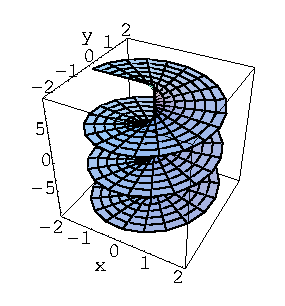
\includegraphics[width=0.25\textwidth]{fcv/function/zarg}
    \end{center}
    \caption{A few branches of the argument function.}
    \label{zarg}
  \end{figure}
  The modulus and principal argument of $f(z) = z$ are plotted in 
  Figure~\ref{zma}.
  \begin{figure}[htbp!]
    \begin{center}
        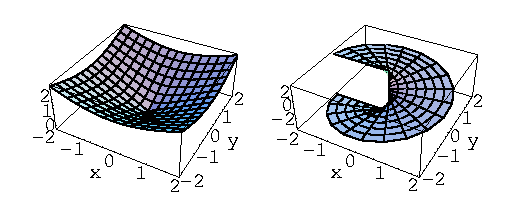
\includegraphics[width=0.5\textwidth]{fcv/function/zma}
    \end{center}
    \caption{Plots of the modulus and argument of \textit{z}.}
    \label{zma}
  \end{figure}
\end{Example}







\begin{Example}
  Consider the function $f(z) = z^2$.  In Cartesian coordinates and separated
  into its real and imaginary components the function is
  \[
  f(z) = z^2 = (x + \imath y)^2 = \left( x^2 - y^2 \right) + \imath 2 x y.
  \]
  Figure~\ref{zsqrreim} shows surface plots of the real and imaginary parts
  of $z^2$.
  \begin{figure}[htbp!]
    \begin{center}
        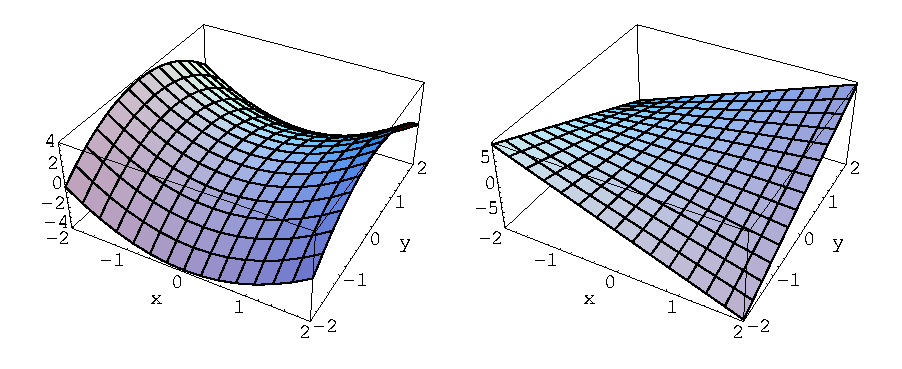
\includegraphics[width=0.8\textwidth]{fcv/function/zsqrreim}
    \end{center}
    \caption{Plots of the real and imaginary parts.}
    \label{zsqrreim}
  \end{figure}
  The magnitude of $z^2$ is
  \[
  |z^2| = \sqrt{z^2 \overline{z^2} } = z \overline{z} 
  = (x + \imath y) (x - \imath y) = x^2 + y^2.
  \]
  Note that 
  \[
  z^2 = \left( r \e^{\imath \theta} \right)^2 = r^2 \e^{\imath 2 \theta}.
  \]
  In Figure~\ref{zsqrma} are plots of $|z^2|$ and a branch of 
  $\arg \left( z^2 \right)$.
  \begin{figure}[htbp!]
    \begin{center}
      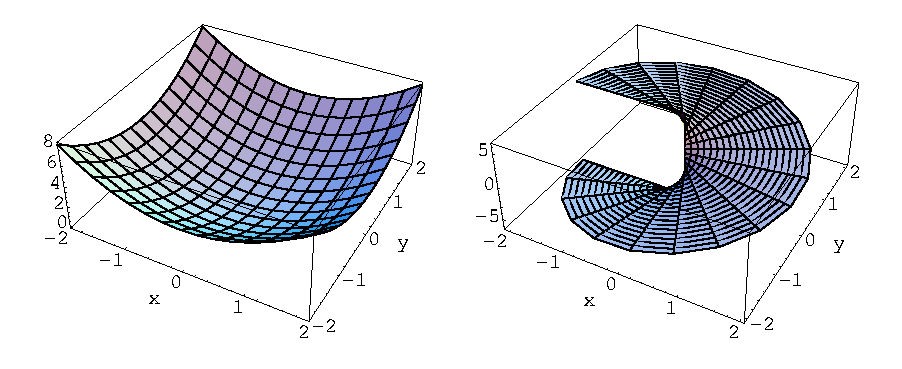
\includegraphics[width=0.8\textwidth]{fcv/function/zsqrma}
    \end{center}
    \caption{Plots of the modulus and a branch of the argument.}
    \label{zsqrma}
  \end{figure}
\end{Example}























%%=============================================================================
\section{Trigonometric Functions}




\paragraph{The exponential function.}
Consider the exponential function $\e^z$.  
We can use Euler's formula to write $\e^z = \e^{x + \imath y}$ in terms of its 
real and imaginary parts. 
\[
\e^z = \e^{x + \imath y} = \e^x \e^{\imath y} = \e^x \cos y + \imath \e^x \sin y
\]
From this we see that the exponential function is $\imath 2 \pi$ periodic:  
$\e^{z + \imath 2 \pi} = \e^z$, and $\imath \pi$ odd periodic: $\e^{z + \imath \pi} = -\e^z$.
Figure~\ref{expreim} has surface plots of the real and imaginary parts
of $\e^z$ which show this periodicity.
\begin{figure}[htbp!]
  \begin{center}
    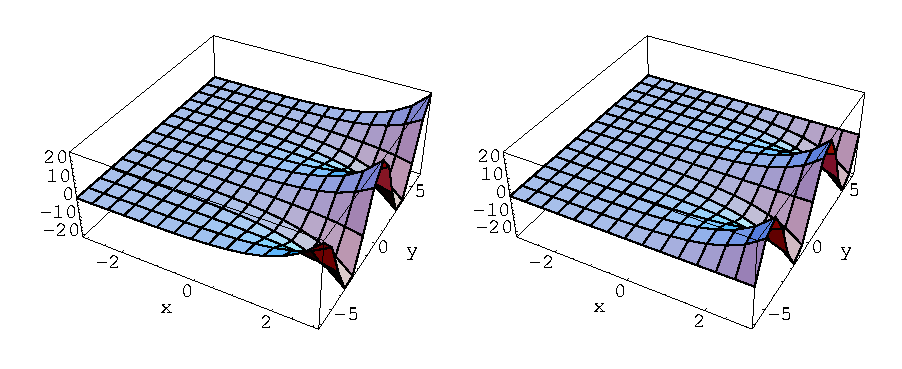
\includegraphics[width=0.8\textwidth]{fcv/function/expreim}
  \end{center}
  \caption{Plots of the real and imaginary parts.}
  \label{expreim}
\end{figure}

The modulus of $\e^z$ is a function of $x$ alone.
\[
\left| \e^z \right| = \left| \e^{x + \imath y} \right| = \e^x
\]
The argument of $\e^z$ is a function of $y$ alone.
\[
\arg \left( \e^z \right) = \arg \left( \e^{x + \imath y} \right) = 
\{ y + 2 \pi n \mid n \in \mathbb{Z} \} 
\]
In Figure~\ref{expma} are plots of $|\e^z|$ and a branch of 
$\arg \left( \e^z \right)$.
\begin{figure}[htbp!]
  \begin{center}
    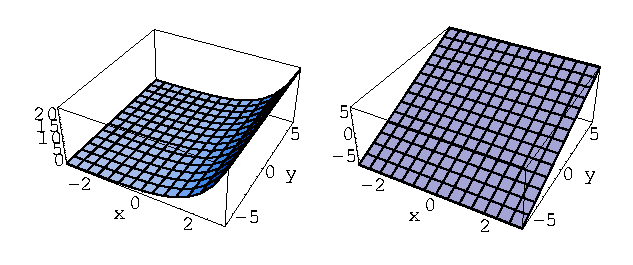
\includegraphics[width=0.6\textwidth]{fcv/function/expma}
  \end{center}
  \caption{Plots of the modulus and a branch of the argument.}
  \label{expma}
\end{figure}







\begin{Example}
  Show that the transformation $w = \e^z$ maps the infinite strip,
  $-\infty < x < \infty$, $0 < y < \pi$, onto the upper half-plane.

  \textbf{Method 1.}
  Consider the line $z = x + \imath c$, $-\infty < x < \infty$.  Under the
  transformation, this is mapped to
  \[ 
  w = \e^{x + \imath c} = \e^{\imath c} \e^x, \quad -\infty < x < \infty. 
  \]
  This is a ray from the origin to infinity in the direction of $\e^{\imath c}$.
  Thus we see that $z = x$ is mapped to the positive, real $w$ axis,
  $z = x + \imath \pi$ is mapped to the negative, real axis, and
  $z = x + \imath c$, $0 < c < \pi$ is mapped to a ray with angle $c$
  in the upper half-plane.  Thus the strip is mapped to the upper half-plane.
  See Figure~\ref{ez_upper_1}.

  \begin{figure}[htbp!]
    \begin{center}
      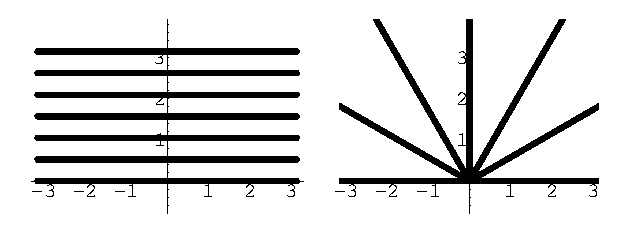
\includegraphics[width=0.6\textwidth]{fcv/function/ez_upper_1}
    \end{center}
    \caption{Horizontal lines are mapped to rays.}
    \label{ez_upper_1}
  \end{figure}

  \textbf{Method 2.}
  Consider the line $z = c + \imath y$, $0 < y < \pi$.  Under the transformation,
  this is mapped to
  \[ 
  w = \e^{c + \imath y} + \e^c \e^{\imath y}, \quad 0 < y < \pi. 
  \]
  This is a semi-circle in the upper half-plane of radius $\e^c$.  As
  $c \to -\infty$, the radius goes to zero.  As $c \to \infty$, the radius
  goes to infinity.  Thus the strip is mapped to the upper half-plane.
  See Figure~\ref{ez_upper_2}.

  \begin{figure}[htbp!]
    \begin{center}
      \includegraphics[width=0.6\textwidth]{fcv/function/ez_upper_2}
    \end{center}
    \caption{Vertical lines are mapped to circular arcs.}
    \label{ez_upper_2}
  \end{figure}

\end{Example}









\paragraph{The sine and cosine.}
We can write the sine and cosine in terms of the exponential function.
\begin{align*}
  \frac{ \e^{\imath z} + \e^{-\imath z} }{ 2 }
  &= \frac{ \cos(z) + \imath \sin(z) + \cos(-z) + \imath \sin(-z) }{ 2 } 
  \\
  &= \frac{ \cos(z) + \imath \sin(z) + \cos(z) - \imath \sin(z) }{ 2 } 
  \\
  &= \cos z
\end{align*}
\begin{align*}
  \frac{ \e^{\imath z} - \e^{-\imath z} }{ \imath 2 }
  &= \frac{ \cos(z) + \imath \sin(z) - \cos(-z) - \imath \sin(-z) }{ 2 } 
  \\
  &= \frac{ \cos(z) + \imath \sin(z) - \cos(z) + \imath \sin(z) }{ 2 } 
  \\
  &= \sin z
\end{align*}
We separate the sine and cosine into their real and imaginary parts.
%% CONTINUE cite an exercise.
\[
\cos z = \cos x \cosh y - \imath \sin x \sinh y \qquad
\sin z = \sin x \cosh y + \imath \cos x \sinh y
\]
For fixed $y$, the sine and cosine are oscillatory in $x$.  The amplitude 
of the oscillations grows with increasing $|y|$.  See 
Figure~\ref{cosreim} and Figure~\ref{sinreim} for plots of the real
and imaginary parts of the cosine and sine, respectively.  
Figure~\ref{cosmsinm} shows the modulus of the cosine and the sine.

\begin{figure}[htbp!]
  \begin{center}
    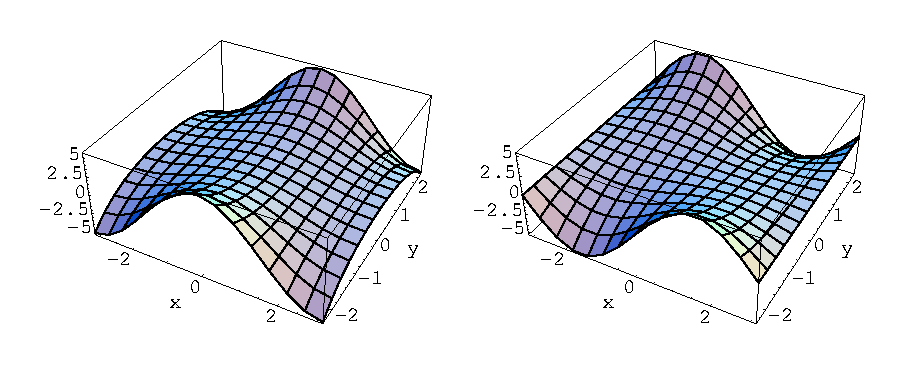
\includegraphics[width=0.8\textwidth]{fcv/function/cosreim}
  \end{center}
  \caption{Plots of the real and imaginary parts of the cosine.}
  \label{cosreim}
\end{figure}

\begin{figure}[htbp!]
  \begin{center}
    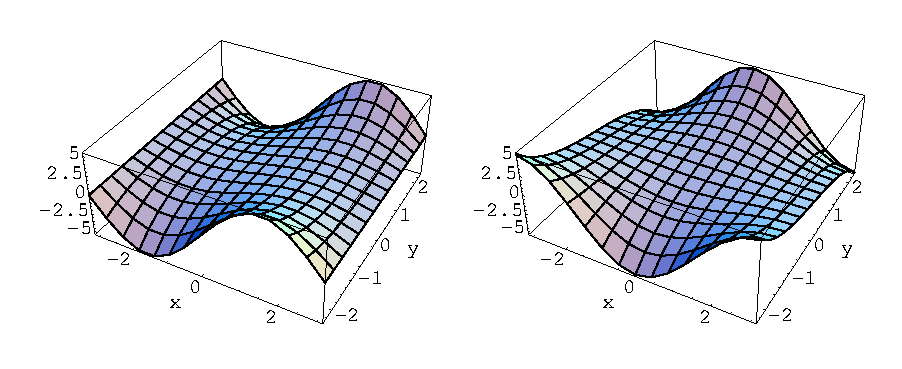
\includegraphics[width=0.8\textwidth]{fcv/function/sinreim}
  \end{center}
  \caption{Plots of the real and imaginary parts of the sine.}
  \label{sinreim}
\end{figure}

\begin{figure}[htbp!]
  \begin{center}
    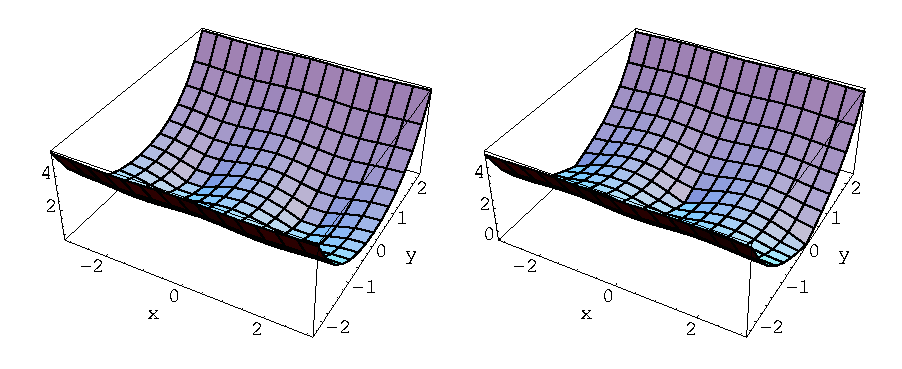
\includegraphics[width=0.8\textwidth]{fcv/function/cosmsinm}
  \end{center}
  \caption{Plots of the modulus of the cosine and the sine.}
  \label{cosmsinm}
\end{figure}



\paragraph{The hyperbolic sine and cosine.}
The hyperbolic sine and cosine have the familiar definitions in terms of the 
exponential function.  Thus not surprisingly, we can write the sine
in terms of the hyperbolic sine and write the cosine in terms of the
hyperbolic cosine.  Below is a collection of trigonometric identities.




\begin{Result}
  \begin{gather*}
    \e^z = \e^x (\cos y + \imath \sin y) 
    \\
    \cos z = \frac{\e^{\imath z} + \e^{-\imath z}}{2} 
    \qquad 
    \sin z = \frac{\e^{\imath z} - \e^{-\imath z}}{\imath 2} 
    \\
    \cos z = \cos x \cosh y - \imath \sin x \sinh y 
    \qquad
    \sin z = \sin x \cosh y + \imath \cos x \sinh y 
    \\
    \cosh z = \frac{\e^z + \e^{-z}}{2} 
    \qquad
    \sinh z = \frac{\e^z - \e^{-z}}{2} 
    \\
    \cosh z = \cosh x \cos y + \imath \sinh x \sin y 
    \qquad
    \sinh z = \sinh x \cos y + \imath \cosh x \sin y 
    \\
    \sin(\imath z) = \imath \sinh z  \qquad \sinh(\imath z) = \imath \sin z 
    \\
    \cos(\imath z) = \cosh z    \qquad \cosh(\imath z) = \cos z 
    \\
    \log z = \ln |z| + \imath \arg(z) 
    = \ln |z| + \imath \Arg(z) + \imath 2 \pi n, \quad n \in \mathbb{Z}
  \end{gather*}
\end{Result}





















%%=============================================================================
\section{Inverse Trigonometric Functions}



\paragraph{The logarithm.}
The logarithm, $\log(z)$, is defined as the inverse of the exponential 
function $\e^z$.  The exponential function is many-to-one and thus 
has a multi-valued inverse.  From what we know of many-to-one functions, we 
conclude that 
\[
\e^{\log z} = z, \quad \mathrm{but} \quad \log \left( \e^z \right) \neq z.
\]
This is because $\e^{\log z}$ is single-valued but $\log \left( \e^z \right)$ is not.
Because $\e^z$ is $\imath 2 \pi$ periodic, the logarithm of a number is 
a set of numbers which differ by integer multiples of $\imath 2 \pi$.  For 
instance, $\e^{\imath 2 \pi n} = 1$ so that 
$\log(1) = \{ \imath 2 \pi n : n \in \mathbb{Z} \}$.
The logarithmic function has an infinite number of branches.  The value of 
the function on the branches differs by integer multiples of $\imath 2 \pi$.  It has 
singularities at zero and infinity.  $|\log(z)| \to \infty$ as either
$z \to 0$ or $z \to \infty$.  

We will derive the formula for the complex variable logarithm.
For now, let $\ln(x)$ denote the real variable logarithm that is defined
for positive real numbers.   Consider $w = \log z$.  This means that
$\e^w = z$.   We write $w = u + \imath v$ in Cartesian form and 
$z = r \e^{\imath \theta}$ in polar form.
\[
\e^{u + \imath v} = r \e^{\imath \theta}
\]
We equate the modulus and argument of this expression.
\begin{gather*}
  \e^u = r \qquad v = \theta + 2 \pi n 
  \\
  u = \ln r \qquad v = \theta + 2 \pi n 
\end{gather*}
With $\log z = u + \imath v$, we have a formula for the logarithm.
\[
\boxed{
  \log z = \ln |z| + \imath \arg(z)
  }
\]
If we write out the multi-valuedness of the argument function we note 
that this has the form that we expected.
\[
\log z = \ln |z| + \imath ( \Arg(z) + 2 \pi n ), \quad n \in \mathbb{Z}
\]
We check that our formula is correct by showing that $\e^{\log z} = z$
\[
\e^{\log z} = \e^{\ln |z| + \imath \arg(z)}
= \e^{\ln r + \imath \theta + \imath 2 \pi n}
= r \e^{\imath \theta}
= z
\]
Note again that $\log \left( \e^z \right) \neq z$.
\[
\log \left( \e^z \right) = \ln |\e^z| + \imath \arg \left( \e^z \right)
= \ln \left( \e^x \right) + \imath \arg \left( \e^{x + \imath y} \right)
= x + \imath (y + 2 \pi n)
= z + \imath 2 n \pi 
\neq z
\]

The real part of the logarithm is the single-valued $\ln r$; 
the imaginary part is the multi-valued $\arg(z)$.
We define the principal branch of the logarithm $\Log z$ to be the branch that 
satisfies $-\pi < \Im(\Log z) \leq \pi$.  For positive, real numbers the
principal branch, $\Log x$ is real-valued.  We can write $\Log z$ in terms of
the principal argument, $\Arg z$.
\[
\Log z = \ln |z| + \imath \Arg(z)
\]
See Figure~\ref{logreim} for plots of the real and imaginary part of 
$\Log z$.

\begin{figure}[htbp!]
  \begin{center}
    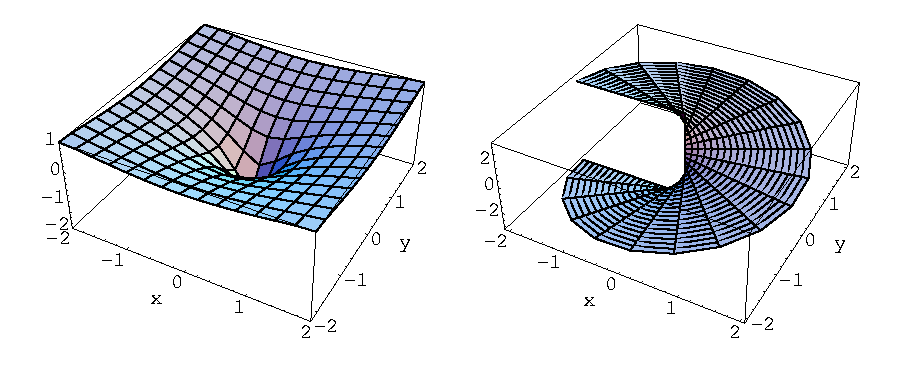
\includegraphics[width=0.8\textwidth]{fcv/function/logreim}
  \end{center}
  \caption{Plots of the real and imaginary parts of the principal branch of
    the logarithm.}
  \label{logreim}
\end{figure}







\paragraph{The form: $\mathbf{a^b}$.}
Consider $a^b$ where $a$ and $b$ are complex and $a$ is nonzero.  We define
this expression in terms of the exponential and the logarithm as
\[
a^b = \e^{b \log a}.
\]
Note that the multi-valuedness of the logarithm may make $a^b$ multi-valued.
First consider the case that the exponent is an integer.
\[
a^m = \e^{m \log a} = \e^{m (\Log a + \imath 2 n \pi)}
= \e^{m \Log a} \e^{\imath 2 m n \pi} = \e^{m \Log a}
\]
Thus we see that $a^m$ has a single value where $m$ is an integer.

Now consider the case that the exponent is a rational number.  Let 
$p/q$ be a rational number in reduced form.
\[
a^{p/q} = \e^{\frac{p}{q} \log a} = \e^{\frac{p}{q}  (\Log a + \imath 2 n \pi)}
= \e^{ \frac{p}{q} \Log a} \e^{\imath 2 n p \pi/q}.
\]
This expression has $q$ distinct values as
\[
\e^{\imath 2 n p \pi / q} = \e^{\imath 2 m p \pi / q} \quad \mathrm{if and only if} \quad
n = m \mod q.
\]

Finally consider the case that the exponent $b$ is an irrational number.
\[
a^b = \e^{b \log a} = \e^{b (\Log a + \imath 2 n \pi) }
= \e^{b \Log a} \e^{\imath 2 b n \pi}
\]
Note that $\e^{\imath 2 b n \pi}$ and
$\e^{\imath 2 b m \pi}$ are equal if and only if $\imath 2 b n \pi$ and $\imath 2 b m \pi$ 
differ by an integer multiple of $\imath 2 \pi$, which means that $b n$ and $b m$ 
differ by an integer.  This occurs only when $n = m$.  Thus $\e^{\imath 2 b n \pi}$
has a distinct value for each different integer $n$.  We conclude that
$a^b$ has an infinite number of values.

You may have noticed something a little fishy.  If $b$ is not an integer
and $a$ is any non-zero complex number, then $a^b$ is multi-valued.
Then why have we been treating $\e^b$ as single-valued, when it is 
merely the case $a = e$?  The answer is that in the realm of functions 
of a complex variable, $\e^z$ is an abuse of notation.  
We write $\e^z$ when we mean $\exp(z)$, the single-valued
exponential function.  Thus when we write $\e^z$ we do not mean 
``the number $e$ raised to the $z$ power'', 
we mean ``the exponential function of $z$''.
We denote the former scenario as $(e)^z$, which is multi-valued.








\paragraph{Logarithmic identities.}
Back in high school trigonometry when you thought that the logarithm was
only defined for positive real numbers you learned the identity
$\log x^a = a \log x$.  This identity doesn't hold when the logarithm is
defined for nonzero complex numbers.  Consider the logarithm of $z^a$.
\[
\log z^a = \Log z^a + \imath 2 \pi n
\]
\[
a \log z = a ( \Log z + \imath 2 \pi n ) = a \Log z + \imath 2 a \pi n
\]
Note that
\[
\log z^a \neq a \log z
\]
Furthermore, since
\[
\Log z^a = \ln |z^a| + \imath \Arg \left( z^a \right), \quad
a \Log z = a \ln |z| + \imath a \Arg(z)
\]
and $\Arg \left( z^a \right)$ is not necessarily the same as $a \Arg(z)$ 
we see that
\[ 
\Log z^a \neq a \Log z. 
\]



Consider the logarithm of a product.
\begin{align*}
  \log(a b) 
  &= \ln |a b| + \imath \arg(a b) 
  \\
  &= \ln |a| + \ln |b| + \imath \arg(a) + \imath \arg(b) 
  \\
  &= \log a + \log b
\end{align*}
There is not an analogous identity for the principal branch of the 
logarithm since $\Arg(a b)$ is not in general the same as 
$\Arg(a) + \Arg(b)$.

Using $\log(a b) = \log(a) + \log(b)$ we can deduce that
$\log \left( a^n \right) = \sum_{k=1}^n \log a = n \log a$, 
where $n$ is a positive integer.
This result is simple, straightforward and wrong.  I have led you down the
merry path to damnation.%
\footnote{
  Don't feel bad if you fell for it.  The logarithm is a 
  tricky bastard.
  }
In fact, $\log \left( a^2 \right) \neq 2 \log a$.  Just write the multi-valuedness
explicitly,
\[
\log \left( a^2 \right) = \Log \left( a^2 \right) + \imath 2 n \pi, \qquad
2 \log a = 2 (\Log a + \imath 2 n \pi) = 2 \Log a + \imath 4 n \pi.
\]


You can verify that 
\[
\log \left( \frac{1}{a} \right) = - \log a.
\]
We can use this and the product identity to expand the logarithm of 
a quotient.
\[
\log \left( \frac{a}{b} \right) = \log a - \log b
\]


For general values of $a$, $\log z^a \neq a \log z$.  However, for some values of 
$a$, equality holds.  We already know that $a = 1$ and $a = -1$ work.  To
determine if equality holds for other values of $a$, we explicitly write the
multi-valuedness.
\begin{gather*}
  \log z^a = \log \left( \e^{a \log z} \right) 
  = a \log z + \imath 2 \pi k, \quad k \in \mathbb{Z} 
  \\
  a \log z = a \ln |z| + \imath a \Arg z + \imath a 2 \pi m, \quad m \in \mathbb{Z}
\end{gather*}
We see that $\log z^a = a \log z$ if and only if
\[
\{ a m \mid m \in \mathbb{Z} \} = \{ a m + k \mid k,m \in \mathbb{Z} \}.
\]
The sets are equal if and only if $a = 1/n$, $n \in \mathbb{Z}^\pm$.  Thus we 
have the identity:
\[
\log \left( z^{1/n} \right) = \frac{1}{n} \log z, \quad n \in \mathbb{Z}^\pm 
\]












\begin{Result}
  \textbf{Logarithmic Identities.}
  \begin{align*}
    &a^b = \e^{b \log a} 
    \\
    &\e^{\log z} = \e^{\Log z} = z 
    \\
    &\log(a b) = \log a + \log b 
    \\
    &\log(1/a) = - \log a 
    \\
    &\log(a/b) = \log a - \log b 
    \\
    &\log \left( z^{1/n} \right) = \frac{1}{n} \log z, \quad n \in \mathbb{Z}^\pm 
  \end{align*}
  \textbf{Logarithmic Inequalities.}
  \begin{align*}
    &\Log(u v) \neq \Log(u) + \Log(v) 
    \\
    &\log z^a \neq a \log z 
    \\
    &\Log z^a \neq a \Log z 
    \\
    &\log \e^z \neq z 
  \end{align*}
\end{Result}









\begin{Example}
  Consider $1^\pi$.  We apply the definition $a^b = \e^{b \log a}$.
  \begin{align*}
    1^\pi    
    &= \e^{\pi \log(1)} 
    \\
    &= \e^{\pi (\ln(1) + \imath 2 n \pi)} 
    \\
    &= \e^{\imath 2 n \pi^2} 
  \end{align*}
  Thus we see that $1^\pi$ has an infinite number of values, all of which
  lie on the unit circle $|z| = 1$ in the complex plane.  However, the set
  $1^\pi$ is not equal to the set $|z| = 1$.  There are points in the 
  latter which are not in the former.  This is analogous to the fact
  that the rational numbers are dense in the real numbers, but are a 
  subset of the real numbers.
\end{Example}







\begin{Example}
  We find the zeros of $\sin z$.

  \begin{gather*}
    \sin z = \frac{\e^{\imath z} - \e^{-\imath z}}{\imath 2} = 0 
    \\
    \e^{\imath z} = \e^{-\imath z} 
    \\
    \e^{\imath 2 z} = 1 
    \\
    2 z \mod 2 \pi = 0 
    \\
    \boxed{ 
      z = n \pi, \quad n \in \mathbb{Z} 
      }
  \end{gather*}

  Equivalently, we could use the identity
  \[ 
  \sin z = \sin x \cosh y + \imath \cos x \sinh y = 0. 
  \]
  This becomes the two equations (for the real and imaginary parts)
  \[ 
  \sin x \cosh y = 0 \qquad \mathrm{and} \qquad \cos x \sinh y = 0. 
  \]
  Since $\cosh$ is real-valued and positive for real argument, 
  the first equation dictates that $x = n \pi$, $n \in \mathbb{Z}$. 
  Since $\cos(n \pi) = (-1)^n$ for $n \in \mathbb{Z}$, the second equation
  implies that $\sinh y = 0$.  For real argument, $\sinh y$ is only zero at
  $y = 0$.  Thus the zeros are
  \[ 
  \boxed{ 
    z = n \pi, \quad n \in \mathbb{Z} 
    } 
  \]
\end{Example}








\begin{Example}
  Since we can express $\sin z$ in terms of the exponential function, one
  would expect that we could express the $\sin^{-1} z$ in terms of the
  logarithm.
  \begin{gather*}
    w =  \sin^{-1} z 
    \\
    z =  \sin w 
    \\
    z =  \frac{\e^{\imath w} - \e^{-\imath w}}{\imath 2} 
    \\
    \e^{\imath 2 w} - \imath 2 z \e^{\imath w} - 1 = 0 
    \\
    \e^{\imath w} =  \imath z \pm \sqrt{1 - z^2} 
    \\
    w =  -\imath \log \left( \imath z \pm \sqrt{1 - z^2} \right)
  \end{gather*}
  Thus we see how the multi-valued $\sin^{-1}$ is related to the logarithm.
  \[
  \boxed{
    \sin^{-1} z =  - \imath \log \left( \imath z \pm \sqrt{1 - z^2} \right)
    }
  \]
\end{Example}











\begin{Example}
  Consider the equation $\sin^3 z = 1$.
  \begin{gather*}
    \sin^3 z = 1 
    \\
    \sin z = 1^{1/3} 
    \\
    \frac{\e^{\imath z} - \e^{-\imath z}}{\imath 2} = 1^{1/3} 
    \\
    \e^{\imath z} - \imath 2 (1)^{1/3} - \e^{-\imath z} = 0 
    \\
    \e^{\imath 2 z} - \imath 2 (1)^{1/3} \e^{\imath z} - 1 = 0 
    \\
    \e^{\imath z} = \frac{\imath 2 (1)^{1/3} \pm \sqrt{-4 (1)^{2/3} + 4}}{2} 
    \\
    \e^{\imath z} = \imath (1)^{1/3} \pm \sqrt{1 - (1)^{2/3}} 
    \\
    \boxed{ 
      z = - \imath \log\left(\imath (1)^{1/3} \pm \sqrt{1 - 1^{2/3}}\right) 
      }
  \end{gather*}
  Note that there are three sources of multi-valuedness in the expression for
  $z$.  The two values of the square root are shown explicitly.  There are
  three cube roots of unity.  Finally, the logarithm has an infinite
  number of branches.  To show this multi-valuedness explicitly, we could write
  \[ 
  \boxed{ 
    z = - \imath \Log\left(\imath \e^{\imath 2 m \pi / 3} \pm \sqrt{1 - \e^{\imath 4 m \pi / 3}}\right)
    + 2 \pi n, \qquad m = 0, 1, 2, \quad n = \ldots, -1, 0, 1, \ldots 
    } 
  \]
\end{Example}









\begin{Example}
  Consider the harmless looking equation, $\imath^z = 1$.

  Before we start with the algebra, note that the right side of the equation
  is a single number.  $\imath^z$ is single-valued only when $z$ is an integer.
  Thus we know that if there are solutions for $z$, they are integers.
  We now proceed to solve the equation.
  \begin{gather*}
    \imath^z = 1 
    \\
    \left( \e^{\imath \pi / 2} \right)^z = 1 
    \\
    \intertext{Use the fact that $z$ is an integer.}
    \e^{\imath \pi z / 2} = 1 
    \\
    \imath \pi z / 2 = \imath 2 n \pi, \quad \mathrm{for some}\ n \in \mathbb{Z} 
    \\
    \boxed{
      z = 4 n, \quad n \in \mathbb{Z}
      }
  \end{gather*}

  Here is a different approach.  We write down the multi-valued form of $\imath^z$.
  We solve the equation by requiring that all the values of $\imath^z$ are $1$.
  \begin{gather*}
    \imath^z = 1 
    \\
    \e^{z \log \imath} = 1 
    \\
    z \log \imath = \imath 2 \pi n, \quad \mathrm{for some}\ n \in \mathbb{Z} 
    \\
    z \left( \imath \frac{\pi}{2} + \imath 2 \pi m \right) = \imath 2 \pi n, \quad \forall 
    m \in \mathbb{Z}, \quad \mathrm{for some}\ n \in \mathbb{Z} 
    \\
    \imath \frac{\pi}{2} z + \imath 2 \pi m z = \imath 2 \pi n, \quad \forall m \in \mathbb{Z},
    \quad \mathrm{for some}\ n \in \mathbb{Z} 
  \end{gather*}
  The only solutions that satisfy the above equation are
  \[
  \boxed{
    z = 4 k, \quad k \in \mathbb{Z}.
    }
  \]

  Now let's consider a slightly different problem: $1 \in \imath^z$.  
  For what values of $z$ does $\imath^z$ have $1$ as one of its values.
  \begin{gather*}
    1 \in \imath^z 
    \\
    1 \in \e^{z \log \imath} 
    \\
    1 \in \{ \e^{z (\imath \pi / 2 + \imath 2 \pi n)} \mid n \in \mathbb{Z} \} 
    \\
    z (\imath \pi / 2 + \imath 2 \pi n) = \imath 2 \pi m, \quad m,n \in \mathbb{Z} 
    \\
    \boxed{
      z = \frac{4 m}{1 + 4 n}, \quad m,n \in \mathbb{Z}
      }
  \end{gather*}
  There are an infinite set of rational numbers for which $\imath^z$ has $1$ as one
  of its values.  For example,
  \[
  \imath^{4/5} = 1^{1/5} =
  \left\{ 1, \e^{\imath 2 \pi / 5}, \e^{\imath 4 \pi / 5}, \e^{\imath 6 \pi / 5}, \e^{\imath 8 \pi / 5} \right\}
  \]
\end{Example}











%%=============================================================================
\section{Riemann Surfaces}

Consider the mapping $w = \log(z)$.  Each nonzero point in the 
$z$-plane is mapped to an infinite number of points in the $w$ plane.
\[
w = \{ \ln |z| + \imath \arg(z) \} 
= \{ \ln |z| + \imath (\Arg(z) + 2 \pi n) \mid n \in \mathbb{Z} \} 
\]
This multi-valuedness makes it hard to work with the logarithm.  We would
like to select one of the branches of the logarithm.  One way of doing 
this is to decompose the $z$-plane into an infinite number of sheets.
The sheets lie above one another and are labeled with the integers, 
$n \in \mathbb{Z}$.  (See Figure~\ref{figure flat-sheets}.)
We label the point $z$ on the $n^{\mathrm{th}}$ sheet as $(z,n)$.  Now each
point $(z,n)$ maps to a single point in the $w$-plane.  For instance,
we can make the zeroth sheet map to the principal branch of the logarithm.
This would give us the following mapping.
\[
\log (z,n) = \Log z + \imath 2 \pi n
\]

\begin{figure}[htbp!]
  \begin{center}
    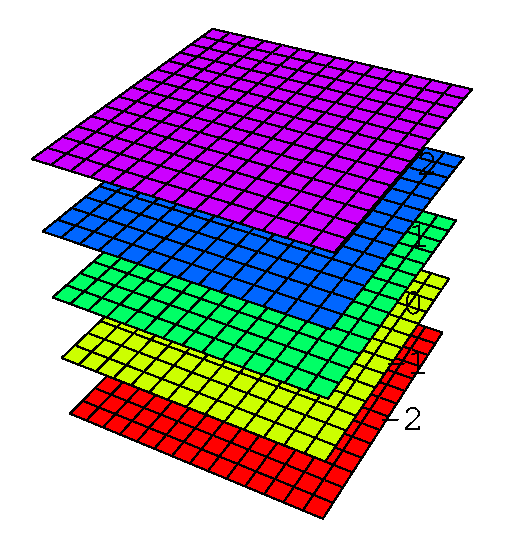
\includegraphics[width=0.3\textwidth]{fcv/function/flat-sheets}
  \end{center}
  \caption{The complex plane decomposed into flat sheets.}
  \label{figure flat-sheets}
\end{figure}



This is a nice idea, but it has some problems.  The mappings are not 
continuous.  Consider the mapping on the zeroth sheet.  As we approach
the negative real axis from above $z$ is mapped to $\ln |z| + \imath \pi$
as we approach from below it is mapped to $\ln |z| - \imath \pi$.
(Recall Figure~\ref{logreim}.)  The mapping is not continuous across the 
negative real axis.

Let's go back to the regular $z$-plane for a moment.
We start at the point $z = 1$ and selecting the branch of the logarithm
that maps to zero.  ($\log(1) = \imath 2 \pi n$).  We make the logarithm
vary continuously as we walk around the origin once in the positive 
direction and return to the point $z = 1$.  Since the argument of $z$
has increased by $2 \pi$, the value of the logarithm has changed to
$\imath 2 \pi$.  If we walk around the origin again we will have 
$\log(1) = \imath 4 \pi$.  Our flat sheet decomposition of the $z$-plane
does not reflect this property.  We need a decomposition with a 
geometry that makes the mapping continuous and connects the various 
branches of the logarithm.


Drawing inspiration from the plot of $\arg(z)$, Figure~\ref{zarg}, we 
decompose the $z$-plane into an infinite corkscrew with axis at the 
origin.  (See Figure~\ref{figure riemann-logz}.)   We define the mapping
so that the logarithm varies continuously on this surface.  
Consider a point $z$ on one of the sheets.  The value of the logarithm 
at that same point on the sheet directly above it is $\imath 2 \pi$ more than 
the original value.  We call this surface, the 
\textit{Riemann surface} for the logarithm.  The mapping from the
Riemann surface to the $w$-plane is continuous and one-to-one.

\begin{figure}[htbp!]
  \begin{center}
    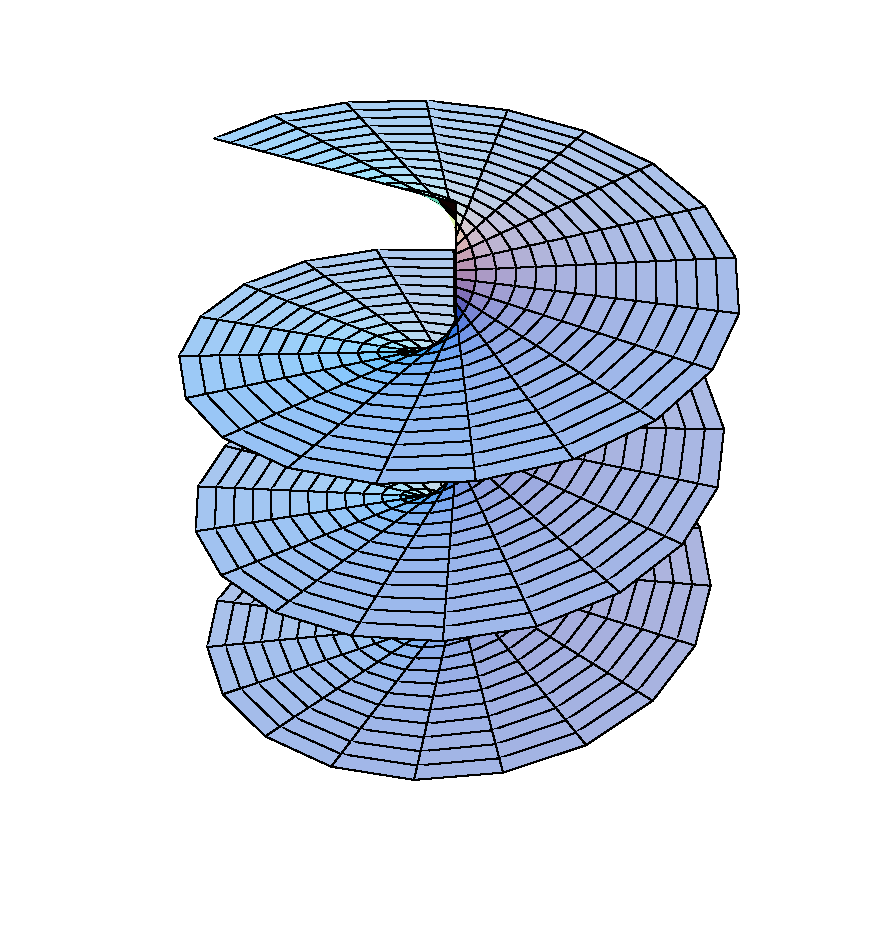
\includegraphics[width=0.3\textwidth]{fcv/function/riemann-logz}
  \end{center}
  \caption{The Riemann surface for the logarithm.}
  \label{figure riemann-logz}
\end{figure}







%%=============================================================================
\section{Branch Points}
\label{chapter function section branch points}
\index{branch point}


%% CONTINUE
%% Before this section:
%% First introduce multi-valuedness in the context of inverse functions of
%% many-to-one mappings.



%% CONTINUE
%% Discover that some multi-valued functions have branch points.






\begin{Example}
  Consider the function $z^{1/2}$.  For each value of $z$, there are
  two values of $z^{1/2}$.  We write $z^{1/2}$ in modulus-argument and 
  Cartesian form.
  \begin{gather*}
    z^{1/2} = \sqrt{|z|} \e^{\imath \arg(z) / 2} 
    \\
    z^{1/2} = \sqrt{|z|} \cos(\arg(z) / 2) + \imath \sqrt{|z|} \sin(\arg(z) / 2)
  \end{gather*}
  Figure~\ref{z_12_re_im} shows the real and imaginary
  parts of $z^{1/2}$ from three different viewpoints.  The second and
  third views are looking down the $x$ axis and $y$ axis,
  respectively.  Consider $\Re \left( z^{1/2} \right)$.  This is a
  double layered sheet which intersects itself on the negative real
  axis.  ($\Im(z^{1/2})$ has a similar structure, but intersects itself
  on the positive real axis.)  Let's start at a point on the positive
  real axis on the lower sheet.  If we walk around the origin once and
  return to the positive real axis, we will be on the upper sheet.  If
  we do this again, we will return to the lower sheet.

  Suppose we are at a point in the complex plane.  We pick one of the
  two values of $z^{1/2}$.  If the function varies continuously as we
  walk around the origin and back to our starting point, the value of
  $z^{1/2}$ will have changed.  We will be on the other branch.
  Because walking around the point $z = 0$ takes us to a different
  branch of the function, we refer to $z = 0$ as a \textit{branch
  point}.

  \begin{figure}[htbp!]
    \begin{center}
      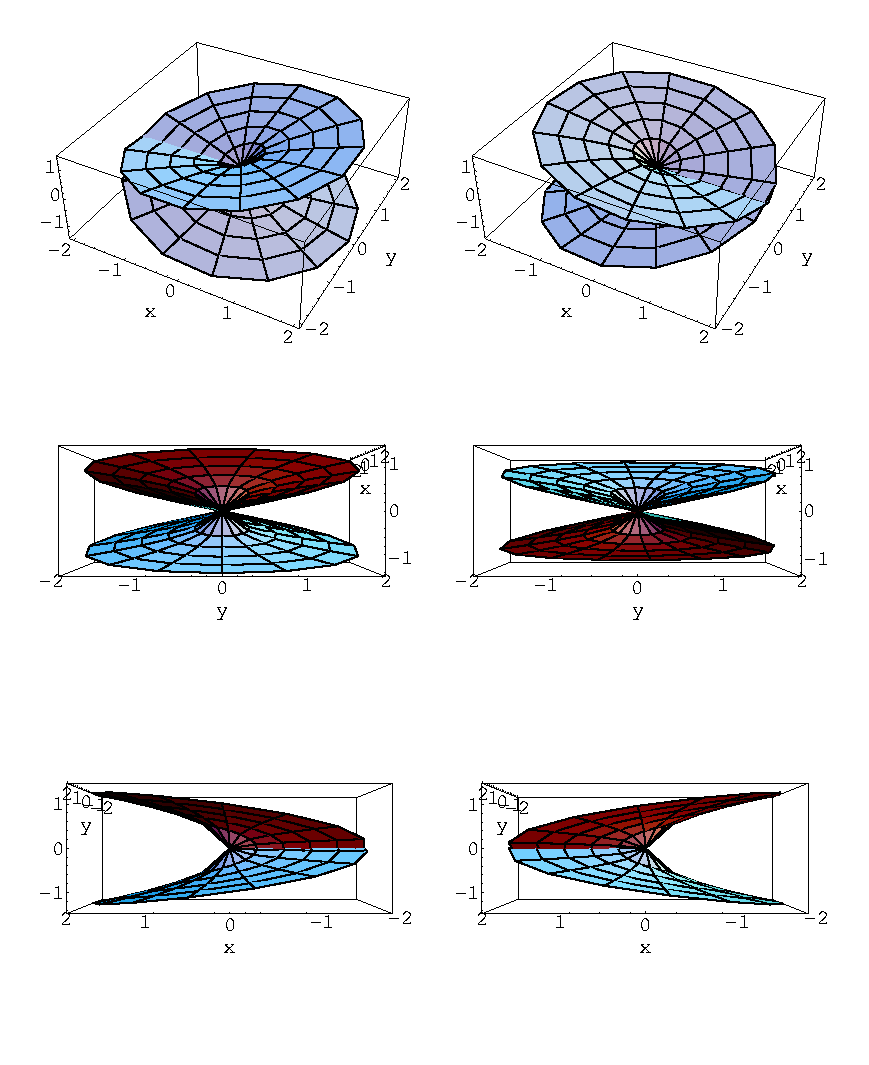
\includegraphics[width=0.55\textwidth]{fcv/function/z_12_re_im}
    \end{center}
    \caption{Plots of the real (left) and 
      imaginary (right) parts from three viewpoints.}
    \label{z_12_re_im}
  \end{figure}

  Now consider the modulus-argument form of $z^{1/2}$:
  \[
  z^{1/2} = \sqrt{|z|} \e^{\imath \arg(z) / 2}.
  \]
  Figure~\ref{z_12_ma} shows the modulus and the principal argument of $z^{1/2}$.
  We see that each time we walk around the origin, the argument of $z^{1/2}$
  changes by $\pi$.  This means that the value of the function changes
  by the factor $\e^{\imath \pi} = -1$, i.e. the function changes sign.  
  If we walk around the origin twice, the argument
  changes by $2 \pi$, so that the value of the function does not change,
  $\e^{\imath 2 \pi} = 1$.

  \begin{figure}[htbp!]
    \begin{center}
      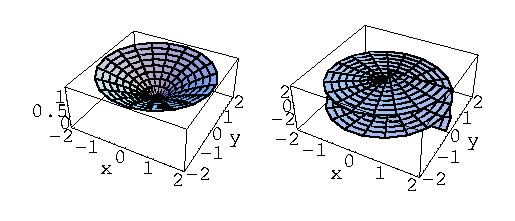
\includegraphics[width=0.5\textwidth]{fcv/function/z_12_ma}
    \end{center}
    \caption{Plots of the modulus and the principal argument.}
    \label{z_12_ma}
  \end{figure}

  $z^{1/2}$ is a continuous function except at
  $z = 0$.  Suppose we start at $z = 1 = \e^{\imath 0}$ and the function value
  $\left( \e^{\imath 0} \right)^{1/2} = 1$.  If we follow the first path in 
  Figure~\ref{unchange_circle_01},
  the argument of $z$
  varies from up to about $\frac{\pi}{4}$, down to about $-\frac{\pi}{4}$
  and back to $0$.  The value of the function is still 
  $\left( \e^{\imath 0} \right)^{1/2}$.

  \begin{figure}[htbp!]
    \begin{center}
      \includegraphics[width=0.5\textwidth]{fcv/function/unchange_change}
    \end{center}
    \caption{A path that does not encircle the origin and a path around 
      the origin.}
    \label{unchange_circle_01}
  \end{figure}

  Now suppose we follow a circular path around the origin in the positive,
  counter-clockwise, direction.  (See the second path in 
  Figure~\ref{unchange_circle_01}.)
  The argument of $z$ increases by $2 \pi$.  The value of the function at
  half turns on the path is
  \begin{align*}
    &\left( \e^{\imath 0} \right)^{1/2} = 1, 
    \\
    &\left( \e^{\imath \pi} \right)^{1/2} = \e^{\imath \pi / 2} = \imath, 
    \\
    &\left( \e^{\imath 2 \pi} \right)^{1/2} = \e^{\imath \pi} = -1
  \end{align*}
  As we return to the point $z = 1$, the argument of the function has changed
  by $\pi$ and the value of the function has changed from $1$ to $-1$.
  If we were to walk along the circular path again, the argument of $z$
  would increase by another $2 \pi$.  The argument of the function would
  increase by another $\pi$ and the value of the function would return to $1$.
  \[
  \left( \e^{\imath 4 \pi} \right)^{1/2} = \e^{\imath 2 \pi} = 1
  \]



  %% CONTINUE: Move this to the next section
  In general, any time we walk around the origin, the value of $z^{1/2}$
  changes by the factor $-1$.  We call $z = 0$ a branch point.  
  If we want a single-valued square root, we need something to prevent us from
  walking around the origin.  We achieve this by introducing a
  branch cut.  Suppose we have the complex plane drawn on an infinite sheet
  of paper. With a scissors we cut the paper from the origin
  to $-\infty$ along the real axis.  Then if we start at $z = \e^{\imath 0}$,
  and draw a continuous line without leaving the paper, the argument of
  $z$ will always be in the range $-\pi < \arg z < \pi$.  This means
  that $-\frac{\pi}{2} < \arg \left( z^{1/2} \right) < \frac{\pi}{2}$.  No matter what
  path we follow in this cut plane, $z = 1$ has argument zero and
  $(1)^{1/2} = 1$.  By never crossing the negative real axis, we have
  constructed a single valued \textbf{branch} of the square root function.
  We call the cut along the negative real axis a \textbf{branch cut}.
\end{Example}






\begin{Example}
  \label{ex_bp_log}
  Consider the logarithmic function $\log z$.  For each value of $z$, there are
  an infinite number of values of $\log z$.  
  We write $\log z$ in Cartesian form.
  \[
    \log z = \ln |z| + \imath \arg z
  \]
  Figure~\ref{logz_reim} shows the real and imaginary parts of the logarithm.
  The real part is single-valued.  The imaginary part is multi-valued and
  has an infinite number of branches.   The values of the logarithm form
  an infinite-layered sheet.  If we start on one of the sheets and walk
  around the origin once in the positive direction, then the value of the
  logarithm increases by $\imath 2 \pi$ and we move to the next branch.
  $z = 0$ is a branch point of the logarithm.

  \begin{figure}[htbp!]
    \begin{center}
      \includegraphics[width=0.6\textwidth]{fcv/function/logz_reim}
    \end{center}
    \caption{Plots of the real part and a portion of imaginary part.}
    \label{logz_reim}
  \end{figure}


  The logarithm is a continuous function except at $z = 0$.  Suppose
  we start at $z = 1 = \e^{\imath 0}$ and the function value $\log\left(
  \e^{\imath 0} \right) = \ln(1) + \imath 0 = 0$.  If we follow the first
  path in Figure~\ref{unchange_circle_01}, the argument of $z$ and
  thus the imaginary part of the logarithm varies from up to about
  $\frac{\pi}{4}$, down to about $-\frac{\pi}{4}$ and back to 0.  The
  value of the logarithm is still $0$.

  Now suppose we follow a circular path around the origin in the positive
  direction.  (See the second path in Figure~\ref{unchange_circle_01}.)
  The argument of $z$ increases by $2 \pi$.  The value of the logarithm at
  half turns on the path is
  \begin{align*}
    &\log\left( \e^{\imath 0} \right) = 0, 
    \\
    &\log\left( \e^{\imath \pi} \right) = \imath \pi, 
    \\
    &\log\left( \e^{\imath 2 \pi} \right) = \imath 2 \pi
  \end{align*}
  As we return to the point $z = 1$, the value of the logarithm has changed
  by $\imath 2 \pi$.
  If we were to walk along the circular path again, the argument of $z$
  would increase by another $2 \pi$ and the value of the logarithm would
  increase by another $\imath 2 \pi$.


  %% CONTINUE: Change to log and Move this to the next section
  %%In general, any time we walk around the origin, the value of $z^{1/2}$
  %%changes by the factor $-1$.  We call $z = 0$ a branch point.  
  %%If we want a single-valued square root, we need something to prevent us from
  %%walking around the origin.  We achieve this by introducing a
  %%branch cut.  Suppose we have the complex plane drawn on an infinite sheet
  %%of paper. With a scissors we cut the paper from the origin
  %%to $-\infty$ along the real axis.  Then if we start at $z = \e^{\imath 0}$,
  %%and draw a continuous line without leaving the paper, the argument of
  %%$z$ will always be in the range $-\pi < \arg z < \pi$.  This means
  %%that $-\frac{\pi}{2} < \arg \left( z^{1/2} \right) < \frac{\pi}{2}$  No matter what
  %%path we follow in this cut plane, $z = 1$ has argument zero and
  %%$(1)^{1/2} = 1$.  By never crossing the negative real axis, we have
  %%constructed a single valued \textbf{branch} of the square root function.
  %%We call the cut along the negative real axis a \textbf{branch cut}.
\end{Example}

















\begin{Result}
  %% CONTINUE
  %% Say this better.
  A point $z_0$ is a \textbf{branch point} of a function $f(z)$ if
  the function changes value when you walk around the point on any
  path that encloses no singularities other than the one at $z = z_0$.
\end{Result}
%% CONTINUE
%% Maybe prove.



\paragraph{Branch points at infinity : mapping infinity to the origin.}
Up to this point we have considered only branch points in the finite
plane.  Now we consider the possibility of a branch point at infinity.
As a first method of approaching this problem we map the point at
infinity to the origin with the transformation $\zeta = 1 / z$ and
examine the point $\zeta = 0$.






\begin{Example}
  Again consider the function $z^{1/2}$.  Mapping the point at infinity to
  the origin, we have $f(\zeta) = (1/\zeta)^{1/2} = \zeta^{-1/2}$.
  For each value of $\zeta$, there are two values of $\zeta^{-1/2}$.  
  We write $\zeta^{-1/2}$ in modulus-argument form.
  \[
  \zeta^{-1/2} = \frac{ 1 }{ \sqrt{|\zeta|} } \e^{- \imath \arg(\zeta) / 2} 
  \]
  Like $z^{1/2}$, $\zeta^{-1/2}$ has a double-layered sheet of values.
  Figure~\ref{zeta_m12_ma} shows the modulus and the principal argument of 
  $\zeta^{-1/2}$.  We see that each time we walk around the origin, the argument
  of $\zeta^{-1/2}$ changes by $-\pi$.  This means that the value of the 
  function changes by the factor $\e^{-\imath \pi} = -1$, i.e. the function changes 
  sign.  If we walk around the origin twice, the argument
  changes by $-2 \pi$, so that the value of the function does not change,
  $\e^{-\imath 2 \pi} = 1$.

  \begin{figure}[htbp!]
    \begin{center}
      \includegraphics[width=0.6\textwidth]{fcv/function/zeta_m12_ma}
    \end{center}
    \caption{Plots of the modulus and the principal argument.}
    \label{zeta_m12_ma}
  \end{figure}

  Since $\zeta^{-1/2}$ has a branch point at zero, we conclude that $z^{1/2}$
  has a branch point at infinity.
\end{Example}









\begin{Example}
  Again consider the logarithmic function $\log z$.  Mapping the point at 
  infinity to the origin, we have $f(\zeta) = \log(1/\zeta) = - \log(\zeta)$.
  From Example~\ref{ex_bp_log} we known that $- \log(\zeta)$ has a branch
  point at $\zeta = 0$.  Thus $\log z$ has a branch point at infinity.
\end{Example}








\paragraph{Branch points at infinity : paths around infinity.}
We can also check for a branch point at infinity by following a path
that encloses the point at infinity and no other singularities.  
Just draw a simple closed curve that separates the complex plane into
a bounded component that contains all the singularities of the function
in the finite plane.  Then, depending on orientation, the curve is 
a contour enclosing all the finite singularities, or the point at 
infinity and no other singularities.



\begin{Example}
  Once again consider the function $z^{1/2}$.  We know that the function 
  changes value on a curve that goes once around the origin.  Such a 
  curve can be considered to be either a path around the origin or a path
  around infinity.  In either case the path encloses one singularity.  
  There are branch points at the origin and at infinity.  Now consider 
  a curve that does not go around the origin.  Such a curve can be considered
  to be either a path around neither of the branch points or both of them.
  Thus we see that $z^{1/2}$ does not change value when we follow a path
  that encloses neither or both of its branch points.
\end{Example}








\begin{Example}
  Consider $f(z) = \left( z^2 - 1 \right)^{1/2}$.  We factor the function.
  \[
  f(z) = (z - 1)^{1/2}  (z + 1)^{1/2}
  \]
  There are branch points at $z = \pm1$.  Now consider the point at infinity.
  \[
  f\left( \zeta^{-1} \right) = \left( \zeta^{-2} - 1 \right)^{1/2} 
  = \pm \zeta^{-1}  \left( 1 - \zeta^2 \right)^{1/2}
  \]
  Since $f\left( \zeta^{-1} \right)$ does not have a branch point at $\zeta = 0$, $f(z)$
  does not have a branch point at infinity.  We could reach the same
  conclusion by considering a path around infinity.  Consider a path
  that circles the branch points at $z = \pm1$ once in the positive
  direction.  Such a path circles the point at infinity once in the
  negative direction.  In traversing this path, the value of $f(z)$ is
  multiplied by the factor 
  $\left( \e^{\imath 2 \pi} \right)^{1/2}  \left( \e^{\imath 2 \pi} \right)^{1/2} = \e^{\imath 2 \pi} = 1$.  
  Thus the value of the function does not
  change.  There is no branch point at infinity.
\end{Example}







\paragraph{Diagnosing branch points.}
We have the definition of a branch point, but we do not have a convenient
criterion for determining if a particular function has a branch point.
We have seen that $\log z$ and $z^\alpha$ for non-integer $\alpha$ have
branch points at zero and infinity.  The inverse trigonometric functions
like the arcsine also have branch points, but they can be written in terms
of the logarithm and the square root.  In fact all the elementary functions
with branch points can be written in terms of the functions $\log z$ and 
$z^\alpha$.  Furthermore, note that the multi-valuedness of $z^\alpha$
comes from the logarithm,  $z^\alpha = \e^{\alpha \log z}$.
This gives us a way of quickly determining if and where a function
may have branch points.


\begin{Result}
  Let $f(z)$ be a single-valued function.  Then $\log(f(z))$ and 
  $(f(z))^\alpha$ may have branch points only where $f(z)$ is zero or singular.
\end{Result}
%% CONTINUE
%% Prove







\begin{Example}
  Consider the functions,
  \begin{enumerate}
  \item $\left( z^2 \right)^{1/2}$
  \item $\left( z^{1/2} \right)^2$
  \item $\left( z^{1/2} \right)^3$
  \end{enumerate}
  Are they multi-valued?  Do they have branch points?

  \begin{enumerate}
  \item
    \[ 
    \left( z^2 \right)^{1/2} = \pm \sqrt{z^2} = \pm z 
    \]
    Because of the $(\cdot)^{1/2}$, the function is multi-valued.  The
    only possible branch points are at zero and infinity.  If
    $\left( \left( \e^{\imath 0} \right)^2 \right)^{1/2} = 1$, then 
    $\left( \left(\e^{\imath 2 \pi} \right)^2 \right)^{1/2} =
    \left( \e^{\imath 4 \pi} \right)^{1/2} = \e^{\imath 2 \pi} = 1$.  Thus we see that
    the function does not change value when we walk around the origin.
    We can also consider this to be a path around infinity.  This
    function is multi-valued, but has no branch points.
  \item
    \[ 
    \left( z^{1/2} \right)^2 = \left( \pm \sqrt{z} \right)^2 = z 
    \]
    This function is single-valued.
  \item
    \[ 
    \left( z^{1/2} \right)^3 = \left( \pm \sqrt{z} \right)^3 
    = \pm \left( \sqrt{z} \right)^3 
    \]
    This function is multi-valued.  
    We consider the possible branch point at $z = 0$.  If 
    $\left( \left( \e^0 \right)^{1/2} \right)^3 = 1$,
    then $\left( \left( \e^{\imath 2 \pi} \right)^{1/2} \right)^3 = \left( \e^{\imath \pi} \right)^3 
    = \e^{\imath 3 \pi} = -1$.  Since
    the function changes value when we walk around the origin,
    it has a branch point at $z = 0$.  Since this is also a path around 
    infinity, there is a branch point there.
  \end{enumerate}
\end{Example}







\begin{Example}
  Consider the function $f(z) = \log \left( \frac{1}{z-1} \right)$.  Since
  $\frac{1}{z-1}$ is only zero at infinity and its only singularity
  is at $z = 1$, the only possibilities for branch points are at $z = 1$
  and $z = \infty$.  Since
  \[
  \log \left( \frac{1}{z-1} \right) = - \log (z-1)
  \]
  and $\log w$ has branch points at zero and infinity, we see that $f(z)$ 
  has branch points at $z = 1$ and $z = \infty$.
\end{Example}






\begin{Example}
  Consider the functions,
  \begin{enumerate}
  \item $\e^{\log z}$
  \item $\log \e^z$. 
  \end{enumerate}
  Are they multi-valued?  Do they have branch points?

  \begin{enumerate}
  \item
    \[ 
    \e^{\log z} = \exp( \Log z + \imath 2 \pi n ) = \e^{\Log z} \e^{\imath 2 \pi n} = z 
    \]
    This function is single-valued.
  \item
    \[ 
    \log \e^z = \Log \e^z + \imath 2 \pi n = z + \imath 2 \pi m 
    \]
    This function is multi-valued.  It may have branch points only where $\e^z$
    is zero or infinite.  This only occurs at $z = \infty$.
    Thus there are no branch points in the finite plane.  The function does
    not change when traversing a simple closed path.  Since this path can
    be considered to enclose infinity, there is no branch point at infinity.
  \end{enumerate}
\end{Example}






Consider $(f(z))^\alpha$ where $f(z)$ is single-valued and $f(z)$ has either a 
zero or a singularity at $z = z_0$.  $(f(z))^\alpha$ may have a branch point at
$z = z_0$.  If $f(z)$ is not a power of $z$, then it may be difficult to tell
if $(f(z))^\alpha$ changes value when we walk around $z_0$.
Factor $f(z)$ into $f(z) = g(z) h(z)$ where $h(z)$ is nonzero and finite 
at $z_0$.  Then $g(z)$ captures the important behavior of $f(z)$ at the 
$z_0$.  $g(z)$ tells us how fast $f(z)$ vanishes or blows up.  
Since $(f(z))^\alpha = (g(z))^\alpha  (h(z))^\alpha$ and $(h(z))^\alpha$
does not have a branch point at $z_0$, $(f(z))^\alpha$ has a 
branch point at $z_0$ if and only if $(g(z))^\alpha$ has a branch point 
there.

Similarly, we can decompose 
\[
\log(f(z)) = \log(g(z) h(z)) = \log(g(z)) + \log(h(z))
\]
to see that $\log(f(z))$ has a branch point at $z_0$ if and only if
$\log(g(z))$ has a branch point there.





\begin{Result}
  Consider a single-valued function $f(z)$ that has either a zero or
  a singularity at $z = z_0$.  Let $f(z) = g(z) h(z)$ where $h(z)$
  is nonzero and finite.  $(f(z))^\alpha$ has a branch point at $z =
  z_0$ if and only if $(g(z))^\alpha$ has a branch point there.
  $\log(f(z))$ has a branch point at $z = z_0$ if and only if
  $\log(g(z))$ has a branch point there.
\end{Result}








\begin{Example}
  Consider the functions,
  \begin{enumerate}
  \item $\sin z^{1/2}$
  \item $(\sin z)^{1/2}$
  \item $z^{1/2} \sin z^{1/2}$
  \item $\left( \sin z^2 \right)^{1/2}$
  \end{enumerate}
  Find the branch points and the number of branches.

  \begin{enumerate}
    %%
    %%
    %%
  \item
    \[ 
    \sin z^{1/2} = \sin \left( \pm \sqrt{z} \right) = \pm \sin \sqrt{z} 
    \]
    $\sin z^{1/2}$ is multi-valued.  It has two branches.
    There may be branch points at zero and infinity.
    Consider the unit circle which is a path around the origin or infinity.
    If $\sin\left( \left( \e^{\imath 0} \right)^{1/2} \right) = \sin(1)$, then
    $\sin\left( \left( \e^{\imath 2 \pi} \right)^{1/2} \right) = \sin\left( \e^{\imath \pi} \right) 
    = \sin (-1) = - \sin(1)$.
    There are branch points at the origin and infinity.
    %%
    %%
    %%
  \item
    \[ 
    (\sin z)^{1/2} = \pm \sqrt{ \sin z } 
    \]
    The function is multi-valued with two branches.  
    The sine vanishes at $z = n \pi$ and is singular at infinity.  
    There could be branch points at these locations.  
    Consider the point $z = n \pi$.  We can write
    \[
    \sin z = (z - n \pi) \frac{\sin z}{z - n \pi}
    \]
    Note that $\frac{\sin z}{z - n \pi}$ is nonzero and has a
    removable singularity at $z = n \pi$.
    \[
    \lim_{z \to n \pi} \frac{\sin z}{z - n \pi} = \lim_{z \to n \pi} \frac{\cos z}{1} = (-1)^n
    \]
    Since $(z - n \pi)^{1/2}$ has a branch point at $z = n \pi$, $(\sin z)^{1/2}$ has 
    branch points at $z = n \pi$.  

    Since the branch points at $z = n \pi$ go all the way out to infinity.
    It is not possible to make a path that encloses infinity and no other
    singularities.  The point at infinity is a non-isolated singularity.
    A point can be a branch point only if it is an isolated singularity.
    %%
    %%
    %%
  \item 
    \begin{align*}
      z^{1/2} \sin z^{1/2}
      &= \pm \sqrt{z} \sin \left( \pm \sqrt{z} \right) 
      \\
      &= \pm \sqrt{z} \left( \pm \sin \sqrt{z} \right) 
      \\
      &= \sqrt{z} \sin \sqrt{z} 
    \end{align*}
    The function is single-valued.  
    Thus there could be no branch points.
    %%
    %%
    %%
  \item
    \[
    \left( \sin z^2 \right)^{1/2} = \pm \sqrt{ \sin z^2 }
    \]
    This function is multi-valued.  Since $\sin z^2 = 0$ at $z = (n \pi)^{1/2}$,
    there may be branch points there.  First consider the point $z = 0$.
    We can write
    \[
    \sin z^2 = z^2 \frac{\sin z^2}{z^2}
    \]
    where  $\sin\left( z^2 \right) / z^2$ is nonzero and has a removable singularity 
    at $z = 0$.
    \[
    \lim_{z \to 0} \frac{\sin z^2}{z^2} = \lim_{z \to 0} \frac{2 z \cos z^2}{2 z} = 1.
    \]
    Since $\left( z^2 \right)^{1/2}$ does not have a branch point at $z = 0$, 
    $\left( \sin z^2 \right)^{1/2}$
    does not have a branch point there either.

    Now consider the point $z = \sqrt{n \pi}$.
    \[
    \sin z^2 = \left( z - \sqrt{n \pi} \right)  \frac{\sin z^2}{z - \sqrt{n \pi}}
    \]
    $\sin\left( z^2 \right) / \left( z - \sqrt{n \pi} \right)$ in nonzero 
    and has a removable singularity at $z = \sqrt{n \pi}$.
    \[
    \lim_{z \to \sqrt{n \pi}} \frac{\sin z^2}{z - \sqrt{n \pi}}
    = \lim_{z \to \sqrt{n \pi}} \frac{2 z \cos z^2}{1}
    = 2 \sqrt{n \pi} (-1)^n
    \]
    Since $\left( z - \sqrt{n \pi} \right)^{1/2}$ has a branch point at $z = \sqrt{n \pi}$,
    $\left( \sin z^2 \right)^{1/2}$ also has a branch point there.

    Thus we see that $\left( \sin z^2 \right)^{1/2}$ has branch points at 
    $z = (n \pi)^{1/2}$ for $n \in \mathbb{Z} \setminus \{0\}$.
    This is the set of numbers: $\{ \pm \sqrt{\pi}, \pm \sqrt{2 \pi}, \ldots,
    \pm \imath \sqrt{\pi}, \pm \imath \sqrt{2 \pi}, \ldots \}$.
    The point at infinity is a non-isolated singularity.
  \end{enumerate}
\end{Example}









\begin{Example}
  Find the branch points of
  \[ 
  f(z) = \left( z^3 - z \right)^{1/3}. 
  \]
  Introduce branch cuts.  If $f(2) = \sqrt[3]{6}$ then what is $f(-2)$?

  We expand $f(z)$.
  \[ 
  f(z) = z^{1/3} (z-1)^{1/3} (z+1)^{1/3}. 
  \]
  There are branch points at $z = -1, 0, 1$.
  We consider the point at infinity.
  \begin{align*}
    f \left( \frac{1}{\zeta} \right)
    &= \left( \frac{1}{\zeta} \right)^{1/3}  \left( \frac{1}{\zeta}  - 1 \right)^{1/3} 
    \left( \frac{1}{\zeta} + 1 \right)^{1/3} 
    \\
    &= \frac{1}{\zeta}  \left( 1 - \zeta \right)^{1/3}  \left( 1 + \zeta \right)^{1/3}
  \end{align*}
  Since $f(1 / \zeta)$ does not have a branch point at $\zeta = 0$, $f(z)$ does 
  not have a branch point at infinity.
  Consider the three possible branch cuts in Figure~\ref{threebc}.

  \begin{figure}[htb!]
    \begin{center}
      \includegraphics[width=0.7\textwidth]{fcv/function/threebc}
    \end{center}
    \caption{Three possible branch cuts.}
    \label{threebc}
  \end{figure}

  The first and the third branch cuts will make the function single valued,
  the second will not.
  It is clear that the first set makes the function single valued since it
  is not possible to walk around any of the branch points.

  The second set of branch cuts would allow you to walk around the branch
  points at $z = \pm 1$.  If you walked around these two once in the positive
  direction, the value of the function would change by the factor
  $\e^{\imath 4 \pi / 3}$.

  The third set of branch cuts would allow you to walk around all three
  branch points together.  You can verify that if you walk around the
  three branch points, the value of the function will not change
  ($\e^{\imath 6 \pi / 3} = \e^{\imath 2 \pi} = 1$).

  Suppose we introduce the third set of branch cuts and
  are on the branch with $f(2) = \sqrt[3]{6}$.
  \[ 
  f(2) = \left( 2 \e^{\imath 0} \right)^{1/3}  \left( 1 \e^{\imath 0} \right)^{1/3} 
  \left( 3 \e^{\imath 0} \right)^{1/3} = \sqrt[3]{6}
  \]
  The value of $f(-2)$ is
  \begin{align*}
    f(-2)   
    &= \left( 2 \e^{\imath \pi} \right)^{1/3}  \left( 3 \e^{\imath \pi} \right)^{1/3}  
    \left( 1 \e^{\imath \pi} \right)^{1/3} 
    \\
    &= \sqrt[3]{2} \e^{\imath \pi/3} \sqrt[3]{3} \e^{\imath \pi/3} \sqrt[3]{1} \e^{\imath \pi/3} 
    \\
    &= \sqrt[3]{6} \e^{\imath \pi} 
    \\
    &= -\sqrt[3]{6}.
  \end{align*}
\end{Example}






\begin{Example}
  Find the branch points and number of branches for
  \[ 
  f(z) = z^{z^2}. 
  \]

  \[
  z^{z^2} = \exp \left( z^2 \log z \right)
  \]
  There may be branch points at the origin and infinity due to the logarithm.
  Consider walking around a circle of radius $r$ centered at the origin in 
  the positive direction.   Since the logarithm changes by $\imath 2 \pi$, the value
  of $f(z)$ changes by the factor $\e^{\imath 2 \pi r^2}$.  
  There are branch points at the origin and infinity.  The function has an
  infinite number of branches.
\end{Example}









\begin{Example}
  Construct a branch of
  \[ 
  f(z) = \left( z^2 + 1 \right)^{1/3} 
  \]
  such that
  \[ 
  f(0) = \frac{1}{2} \left( -1 + \imath \sqrt{3} \right). 
  \]

  First we factor $f(z)$.
  \[ 
  f(z) = (z - \imath)^{1/3}  (z + \imath)^{1/3}
  \]
  There are branch points at $z = \pm \imath$.  Figure~\ref{singvbc} 
  shows one way to introduce branch cuts.

  \begin{figure}[htb!]
    \begin{center}
      \includegraphics[width=0.2\textwidth]{fcv/function/singvbc}
    \end{center}
    \caption{The branch cuts.}
    \label{singvbc}
  \end{figure}

  Since it is not possible to walk around any branch point, these cuts make
  the function single valued.  We introduce the coordinates:
  \[
  z - \imath = \rho \e^{\imath \phi}, \quad z + \imath = r \e^{\imath \theta}.
  \]
  \begin{align*}
    f(z) &= \left( \rho \e^{\imath \phi} \right)^{1/3}  \left( r \e^{\imath \theta} \right)^{1/3} 
    \\
    &= \sqrt[3]{\rho r} \e^{\imath (\phi+\theta)/3}
  \end{align*}

  The condition
  \[ 
  f(0) = \frac{1}{2} \left( -1 + \imath \sqrt{3} \right) = \e^{\imath (2 \pi/3 + 2 \pi n)} 
  \]
  can be stated
  \begin{gather*}
    \sqrt[3]{1} \e^{\imath (\phi + \theta)/3} = \e^{\imath (2 \pi/3 + 2 \pi n)} 
    \\
    \phi + \theta = 2 \pi + 6 \pi n
  \end{gather*}

  The angles must be defined to satisfy this relation.  One choice is
  \[ 
  \boxed{ 
    \frac{\pi}{2} < \phi < \frac{5 \pi}{2}, \quad
    -\frac{\pi}{2} < \theta < \frac{3 \pi}{2}. 
    } 
  \]
\end{Example}









%% CONTINUE: expand

\paragraph{Principal branches.}
We construct the principal branch of the logarithm by putting a branch
cut on the negative real axis choose $z = r \e^{\imath \theta}$, 
$\theta \in (-\pi,\pi)$.
Thus the principal branch of the logarithm is 
\[
\Log z = \ln r + \imath \theta, \qquad -\pi < \theta < \pi.
\]
Note that the if $x$ is a negative real number, (and thus lies on the 
branch cut), then $\Log x$ is undefined.

The principal branch of $z^\alpha$ is
\[
z^\alpha = \e^{\alpha \Log z}.
\]
Note that there is a branch cut on the negative real axis.
\[
-\alpha \pi < \arg\left( \e^{\alpha \Log z} \right) < \alpha \pi
\]

The principal branch of the $z^{1/2}$ is denoted $\sqrt{z}$.  The 
principal branch of $z^{1/n}$ is denoted $\sqrt[n]{z}$.



\begin{Example}
  Construct $\sqrt{1 - z^2}$, the principal branch of 
  $\left( 1 - z^2 \right)^{1/2}$.

  First note that since $\left( 1 - z^2 \right)^{1/2} = (1 - z)^{1/2}  (1 + z)^{1/2}$ 
  there are branch points at $z = 1$ and $z = -1$.
  The principal branch of the square root has a branch cut on the negative
  real axis.  $1 - z^2$ is a negative real number for $z \in (-\infty \ldots -1)
  \cup (1 \ldots \infty)$.  Thus we put branch cuts on $(-\infty \ldots -1]$ and $[1 \ldots \infty)$.
\end{Example}







\raggedbottom
%%=============================================================================
\exercises{
\pagebreak
\flushbottom
\section{Exercises}




%%-----------------------------------------------------------------------------
\begin{large}
  \noindent
  \textbf{Cartesian and Modulus-Argument Form}
\end{large}





\begin{Exercise}
  \label{exercise image z2}
  Find the image of the strip $2 < x < 3$ under the mapping $w = f(z) = z^2$.
  Does the image constitute a domain?

  \hintsolution{image z2}
\end{Exercise}





%% the transformation $w=z^4$
\begin{Exercise}
  \label{exercise z^4}
  For a given real number $\phi$, $0 \leq \phi < 2 \pi$, find the
  image of the sector $0 \leq \arg(z) < \phi$ under the transformation
  $w = z^4$. How large should $\phi$ be so that the $w$ plane is covered
  exactly once?

  \hintsolution{z^4}
\end{Exercise}




%%-----------------------------------------------------------------------------
\begin{large}
  \noindent
  \textbf{Trigonometric Functions}
\end{large}


%% sin(z) in Cartesian and modulus-argument form
\begin{Exercise}
  \label{exercise sin(z) cart mod-arg}
  In Cartesian coordinates, $z = x + \imath y$, write $\sin(z)$ in Cartesian
  and modulus-argument form.

  \hintsolution{sin(z) cart mod-arg}
\end{Exercise}



%% $\e^z$ is nonzero
\begin{Exercise}
  \label{exercise e z nonzero}
  Show that $\e^z$ is nonzero for all finite $z$.

  \hintsolution{e z nonzero}
\end{Exercise}


%% \left| \e^{z^2} \right| \leq \e^{|z|^2}
\begin{Exercise}
  \label{exercise ez lt ez}
  Show that
  \[
  \left| \e^{z^2} \right| \leq \e^{|z|^2}.
  \]
  When does equality hold?

  \hintsolution{ez lt ez}
\end{Exercise}






%% $\coth z = 1$
\begin{Exercise}
  \label{exercise cothz = 1}
  Solve $\coth(z) = 1$.

  \hintsolution{cothz = 1}
\end{Exercise}



%% 2 \in 2^z
\begin{Exercise}
  \label{exercise 2 in 2z}
  Solve $2 \in 2^z$.  That is, for what values of $z$ is $2$ one of the values
  of $2^z$?  Derive this result then verify your answer by evaluating $2^z$
  for the solutions that your find.

  \hintsolution{2 in 2z}
\end{Exercise}




%% 1 \in 1^z
\begin{Exercise}
  \label{exercise 1 in 1z}
  Solve $1 \in 1^z$.  That is, for what values of $z$ is $1$ one of the values
  of $1^z$?  Derive this result then verify your answer by evaluating $1^z$
  for the solutions that your find.

  \hintsolution{1 in 1z}
\end{Exercise}




%%-----------------------------------------------------------------------------
\begin{large}
  \noindent
  \textbf{Logarithmic Identities}
\end{large}






\begin{Exercise}
  \label{exercise Log z1z2}
  Show that if $\Re \left( z_1 \right) > 0$ and $\Re \left( z_2 \right) > 0$ then
  \[
  \Log( z_1 z_2 ) = \Log( z_1 ) + \Log( z_2 )
  \]
  and illustrate that this relationship does not hold in general.

  \hintsolution{Log z1z2}
\end{Exercise}







%% Find the fallacy in the following argument: \log(-1) = 0.
\begin{Exercise}
  \label{exercise log-1 = 0}
  Find the fallacy in the following arguments:
  \begin{enumerate}
  \item
    $\log(-1) = \log \left( \frac{1}{-1} \right) 
    = \log(1) - \log(-1)
    = - \log(-1)$,
    therefore, $\log(-1) = 0$.
  \item
    $1 = 1^{1/2} = ((-1) (-1))^{1/2} = (-1)^{1/2}  (-1)^{1/2} = \imath \imath =  -1$, 
    therefore, $1 = -1$.
  \end{enumerate}

  \hintsolution{log-1 = 0}
\end{Exercise}











%% modulus-argument and Cartesian form for logarithms
\begin{Exercise}
  \label{exercise mod-arg cart log}
  Write the following expressions in modulus-argument or Cartesian form.
  Denote any multi-valuedness explicitly.
  \[
  2^{2/5}, \quad 3^{1 + \imath}, \quad \left( \sqrt{3} - \imath \right)^{1/4}, \quad 1^{\imath / 4}.
  \]

  \hintsolution{mod-arg cart log}
\end{Exercise}



%% $\cos z = 69$.
\begin{Exercise}
  \label{exercise cosz = 69}
  Solve $\cos z = 69$.

  \hintsolution{cosz = 69}
\end{Exercise}



%% $\cot z = \imath 47$.
\begin{Exercise}
  \label{exercise cotz = i47}
  Solve $\cot z = \imath 47$.

  \hintsolution{cotz = i47}
\end{Exercise}





%% $\log(-\imath)$ $(-\imath)^{-\imath}$ $3^{\pi}$
\begin{Exercise}
  \label{exercise log-i}
  Determine all values of 
  \begin{enumerate}
  \item
    $\log(-\imath)$ 
  \item
    $(-\imath)^{-\imath}$ 
  \item
    $3^{\pi}$
  \item
    $\log(\log(\imath))$
  \end{enumerate}
  and plot them in the complex plane.

  \hintsolution{log-i}
\end{Exercise}





\begin{Exercise}
  \label{exercise cosh ip i2}
Evaluate and plot the following in the complex plane:
\begin{enumerate}
\item 
  $\displaystyle
  ( \cosh(\imath \pi) )^{\imath 2}
  $
\item 
  $\displaystyle
  \log \left( \frac{1}{1 + \imath} \right)
  $
\item 
  $\displaystyle
  \arctan(\imath 3)
  $
\end{enumerate}

  \hintsolution{cosh ip i2}
\end{Exercise}





%% Determine all values of $\imath^\imath$ and $\log((1+\imath)^{\imath \pi})$ and plot them
\begin{Exercise}
  \label{exercise ii log1i}
  Determine all values of $\imath^\imath$ and $\log\left( (1+\imath)^{\imath \pi} \right)$ and 
  plot them in the complex plane.

  \hintsolution{ii log1i}
\end{Exercise}







%% $\e^z = \imath$ $\cos z = \sin z$ $\tan^2 z = -1$
\begin{Exercise}
  Find all $z$ for which
  \begin{enumerate}
  \item
    $\e^z = \imath$ 
  \item
    $\cos z = \sin z$ 
  \item
    $\tan^2 z = -1$
  \end{enumerate}

  \hintsolution{ez = i}
\end{Exercise}






%% \tan^{-1}(z) =\frac{\imath}{2} \log\left( \frac{i+z}{i-z}\right)
\begin{Exercise}
  \label{exercise arctan z}
  Prove the following identities
  and identify the branch points of the functions in the extended 
  complex plane.
  \begin{enumerate}
  \item
    $\displaystyle
    \arctan(z) =\frac{\imath}{2} \log\left( \frac{\imath + z}{\imath - z}\right)
    $
  \item
    $\displaystyle
    \arctanh(z) =\frac{1}{2} \log\left( \frac{1 + z}{1 - z}\right)
    $
  \item
    $\displaystyle
    \arccosh(z) = \log \left( z + \left( z^2 - 1 \right)^{1/2} \right)
    $
  \end{enumerate}

  \hintsolution{arctan z}
\end{Exercise}











%%-----------------------------------------------------------------------------
\begin{large}
  \noindent
  \textbf{Branch Points and Branch Cuts}
\end{large}





\begin{Exercise}
  \label{exercise log zz+1z-1}
  Identify the branch points of the function
  \[
  f(z) = \log \left( \frac{ z (z+1) }{ z-1 } \right)
  \]
  and introduce appropriate branch cuts to ensure that the function is 
  single-valued.

  \hintsolution{log zz+1z-1}
\end{Exercise}





\begin{Exercise}
  \label{exercise z3 z2 6z 12}
  Identify all the branch points of the function
  \[
  w = f(z) = \left( z^3 + z^2 - 6 z \right)^{1/2}
  \]
  in the extended complex plane.  Give a polar description of $f(z)$ and 
  specify branch cuts so that your choice of angles gives a single-valued
  function that is continuous at $z = -1$ with $f(-1) = - \sqrt{6}$.
  Sketch the branch cuts in the stereographic projection.

  \hintsolution{z3 z2 6z 12}
\end{Exercise}








\begin{Exercise}
  \label{exercise mapping z13}
  Consider the mapping $w = f(z) = z^{1/3}$ and the inverse mapping 
  $z = g(w) = w^3$.
  \begin{enumerate}
  \item 
    Describe the multiple-valuedness of $f(z)$.
  \item
    Describe a region of the $w$-plane that $g(w)$ maps one-to-one to the whole
    $z$-plane.
  \item
    Describe and attempt to draw a Riemann surface on which $f(z)$ is 
    single-valued and to which $g(w)$ maps one-to-one.  Comment on the 
    misleading nature of your picture.
  \item
    Identify the branch points of $f(z)$ and introduce a branch cut to make 
    $f(z)$ single-valued.
  \end{enumerate}

  \hintsolution{mapping z13}
\end{Exercise}






%% f(z)=(z^3-1)^{1/2}.
\begin{Exercise}
  \label{exercise z3112}
  Determine the branch points of the function
  \[
  f(z) = \left( z^3 - 1 \right)^{1/2}.
  \]
  Construct cuts and define a branch so that $z = 0$ and $z = -1$ do 
  not lie on a
  cut, and such that $f(0) = -\imath$. What is $f(-1)$ for this branch?

  \hintsolution{z3112}
\end{Exercise}





%% w(z) = \left( (z-1)(z-6)(z+2) \right)^{1/2}
\begin{Exercise}
  \label{exercise z1z6z2}
  Determine the branch points of the function
  \[
  w(z) = \left( (z-1) (z-6) (z+2) \right)^{1/2}
  \]
  Construct cuts and define a branch so that $z = 4$ does not lie
  on a cut, and such that $w = \imath 6$ when $z = 4$.

  \hintsolution{z1z6z2}
\end{Exercise}






%% \cos z^{1/2} (z + \imath)^{-z}
\begin{Exercise}
  \label{exercise cos z12}
  Give the number of branches and locations of the branch points for the 
  functions
  \begin{enumerate}
  \item $\displaystyle \cos \left( z^{1/2} \right)$
  \item $\displaystyle (z + \imath)^{-z}$
  \end{enumerate}

  \hintsolution{cos z12}
\end{Exercise}









%%
\begin{Exercise}
  \label{exercise z2112}
  Find the branch points of the following functions in the extended complex
  plane, (the complex plane including the point at infinity).
  \begin{enumerate}
  \item $\displaystyle \left( z^2 + 1 \right)^{1/2}$
  \item $\displaystyle \left( z^3 - z \right)^{1/2}$
  \item $\displaystyle \log \left( z^2 - 1 \right)$
  \item $\displaystyle \log \left( \frac{z+1}{z-1} \right)$
  \end{enumerate}
  Introduce branch cuts to make the functions single valued.

  \hintsolution{z2112}
\end{Exercise}







%% f(z) = \left( z^3 + 8 \right)^{1/2}
\begin{Exercise}
  \label{exercise z3812}
  Find all branch points and introduce cuts to make the following functions
  single-valued:  For the first function, choose cuts so that there is 
  no cut within the disk $|z| < 2$.
  \begin{enumerate}
  \item $\displaystyle f(z) = \left( z^3 + 8 \right)^{1/2}$
  \item $\displaystyle f(z) 
    = \log \left( 5 + \left( \frac{z+1}{z-1} \right)^{1/2} \right)$
  \item $\displaystyle f(z) = (z + \imath 3)^{1/2}$
  \end{enumerate}

  \hintsolution{z3812}
\end{Exercise}






%% branch point at infinity I
\begin{Exercise}
  \label{exercise bp inf 1}
  Let $f(z)$ have branch points at $z = 0$ and $z = \pm \imath$, but nowhere else
  in the extended complex plane.  How does the value and argument of $f(z)$
  change while traversing the contour in Figure~\ref{cont_around_0pmi}?
  Does the branch cut in Figure~\ref{cont_around_0pmi} make the function 
  single-valued?
  \begin{figure}[htbp!]
    \begin{center}
      \includegraphics[width=0.25\textwidth]{fcv/function/cont_around_0pmi}
    \end{center}
    \caption{Contour around the branch points and the branch cut.}
    \label{cont_around_0pmi}
  \end{figure}

  \hintsolution{bp inf 1}
\end{Exercise}






%% branch point at infinity II
\begin{Exercise}
  \label{exercise bp inf 2}
  Let $f(z)$ be analytic except for no more than a countably infinite number
  of singularities.  Suppose that $f(z)$ has only one branch point in the
  finite complex plane.  Does $f(z)$ have a branch point at infinity?
  Now suppose that $f(z)$ has two or more branch points in the finite
  complex plane.  Does $f(z)$ have a branch point at infinity?

  \hintsolution{bp inf 2}
\end{Exercise}





%% $(z^4 + 1)^{1/4}
\begin{Exercise}
  \label{exercise z4114}
  Find all branch points of $\left( z^4 + 1 \right)^{1/4}$ in the extended 
  complex plane.
  Which of the branch cuts in Figure~\ref{fourbc} make the function 
  single-valued.
  \begin{figure}[htbp!]
    \begin{center}
      \includegraphics[width=\textwidth]{fcv/function/fourbc}
    \end{center}
    \caption{Four candidate sets of branch cuts.}
    \label{fourbc}
  \end{figure}

  \hintsolution{z4114}
\end{Exercise}






%%
\begin{Exercise}
  \label{exercise zz21}
  Find the branch points of
  \[
  f(z) = \left( \frac{z}{z^2 + 1} \right)^{1/3}
  \]
  in the extended complex plane.  Introduce branch cuts that make the function
  single-valued and such that the function is defined on the positive
  real axis.  Define a branch such that $f(1) = 1 / \sqrt[3]{2}$.  Write
  down an explicit formula for the value of the branch.  What is $f(1 + \imath)$?
  What is the value of $f(z)$ on either side of the branch cuts?

  \hintsolution{zz21}
\end{Exercise}







%% ((z-1)(z-2)(z-3))^{1/2}
\begin{Exercise}
  \label{exercise z1z2z3}
  Find all branch points of 
  \[
  f(z) = ((z-1)(z-2)(z-3))^{1/2}
  \]
  in the extended complex plane.  Which of the branch cuts in
  Figure~\ref{bpbc123} will make the function single-valued.  Using
  the first set of branch cuts in this figure define a branch on which
  $f(0) = \imath \sqrt{6}$.  Write out an explicit formula for the value
  of the function on this branch.
  \begin{figure}[htbp!]
    \begin{center}
      \includegraphics[width=0.5\textwidth]{fcv/function/bpbc123}
    \end{center}
    \caption{Four candidate sets of branch cuts.}
    \label{bpbc123}
  \end{figure}

  \hintsolution{z1z2z3}
\end{Exercise}






%% w = \left( (z^2 - 2)(z + 2) \right)^{1/3}.
\begin{Exercise}
  \label{exercise z22z2}
  Determine the branch points of the function
  \[
  w = \left( \left( z^2 - 2 \right) (z + 2) \right)^{1/3}.
  \]
  Construct and define a branch so that the resulting cut is one line of 
  finite extent and $w(2) = 2$.  What is $w(-3)$ for this branch?  What are 
  the limiting values of $w$ on either side of the branch cut?

  \hintsolution{z22z2}
\end{Exercise}








%%
\begin{Exercise}
  \label{exercise pb arccos}
  Construct the principal branch of $\arccos(z)$.  ($\Arccos(z)$ has the 
  property that if $x \in [-1,1]$ then $\Arccos(x) \in [0,\pi]$.  In 
  particular, $\Arccos(0) = \frac{\pi}{2}$).

  \hintsolution{pb arccos}
\end{Exercise}





%% (z^{1/2} - 1)^{1/2}
\begin{Exercise}
  \label{exercise bp z12112}
  Find the branch points of $\left( z^{1/2} - 1 \right)^{1/2}$ in the finite complex
  plane.  Introduce branch cuts to make the function single-valued.

  \hintsolution{bp z12112}
\end{Exercise}






%% For the linkage illustrated in 
\begin{Exercise}
  \label{exercise linkage}
  For the linkage illustrated in Figure~\ref{linkage}, 
  use complex variables to outline a scheme for 
  expressing the angular position, velocity and acceleration of arm $c$ in
  terms of those of arm $a$.  (You needn't work out the equations.)
  \begin{figure}[htbp!]
    \begin{center}
      \includegraphics[width=0.4\textwidth]{fcv/function/linkage}
    \end{center}
    \caption{A linkage.}
    \label{linkage}
  \end{figure}

  \hintsolution{linkage}
\end{Exercise}







%% Find the image of the strip $|\Re(z)| < 1$ and of the strip $1 < \Im(z) < 2$
\begin{Exercise}
  \label{exercise image 2z2}
  Find the image of the strip $|\Re(z)| < 1$ and of the strip $1 < \Im(z) < 2$
  under the transformations:
  \begin{enumerate}
  \item
    $w = 2 z^2$
  \item
    $w = \frac{z + 1}{z - 1}$
  \end{enumerate}

  \hintsolution{image 2z2}
\end{Exercise}









%% \frac{(z+1)^{1/2}}{z+2}, \cos \left( \frac{1}{1+z} \right), ...
\begin{Exercise}
  \label{exercise classify z1z2}
  Locate and classify all the singularities of the following functions:
  \begin{enumerate}
  \item $\displaystyle \frac{(z+1)^{1/2}}{z+2}$
  \item $\displaystyle \cos \left( \frac{1}{1+z} \right)$
  \item $\displaystyle \frac{1}{\left( 1 - \e^z \right)^2 }$
  \end{enumerate}
  In each case discuss the possibility of a singularity at the point $\infty$.

  \hintsolution{classify z1z2}
\end{Exercise}








%% Describe how the mapping $w=\sinh(z)$
\begin{Exercise}
  \label{exercise sinh 0 pi}
  Describe how the mapping $w = \sinh(z)$ transforms
  the infinite strip $-\infty < x < \infty$, $0 < y < \pi$ into the
  $w$-plane. Find cuts in the $w$-plane which make the mapping
  continuous both ways. What are the images of the lines (a) $y = \pi / 4$;
  (b) $x = 1$?

  \hintsolution{sinh 0 pi}
\end{Exercise}











\raggedbottom
}
%%=============================================================================
\hints{
\pagebreak
\flushbottom
\section{Hints}





%%-----------------------------------------------------------------------------
\begin{large}
  \noindent
  \textbf{Cartesian and Modulus-Argument Form}
\end{large}





\begin{Hint}
  \label{hint image z2}
  %% CONTINUE
\end{Hint}



%% the transformation $w=z^4$
\begin{Hint}
  \label{hint z^4}
  %% CONTINUE
\end{Hint}



%%-----------------------------------------------------------------------------
\begin{large}
  \noindent
  \textbf{Trigonometric Functions}
\end{large}


%% sin(z) in Cartesian and modulus-argument form
\begin{Hint}
  \label{hint sin(z) cart mod-arg}
  Recall that $\sin(z) = \frac{1}{\imath 2}  \left( \e^{\imath z} - \e^{-\imath z} \right)$.
  Use Result~\ref{cartesian_and_polar_form} to convert between Cartesian
  and modulus-argument form.
\end{Hint}


%% $\e^z$ is nonzero
\begin{Hint}
  \label{hint e z nonzero}
  Write $\e^z$ in polar form.
\end{Hint}




%% \left| \e^{z^2} \right| \leq \e^{|z|^2}
\begin{Hint}
  \label{hint ez lt ez}
  The exponential is an increasing function for real variables.
\end{Hint}







%% $\coth z = 1$
\begin{Hint}
  \label{hint cothz = 1}
  Write the hyperbolic cotangent in terms of exponentials.
\end{Hint}


%% 2 \in 2^z
\begin{Hint}
  \label{hint 2 in 2z}
  Write out the multi-valuedness of $2^z$.  There is a doubly-infinite set of 
  solutions to this problem.
\end{Hint}


%% 1 \in 1^z
\begin{Hint}
  \label{hint 1 in 1z}
  Write out the multi-valuedness of $1^z$.
\end{Hint}





%%-----------------------------------------------------------------------------
\begin{large}
  \noindent
  \textbf{Logarithmic Identities}
\end{large}




\begin{Hint}
  \label{hint Log z1z2}
  %% CONTINUE
\end{Hint}





%% Find the fallacy in the following argument: \log(-1) = 0.
\begin{Hint}
  \label{hint log-1 = 0}
  Write out the multi-valuedness of the expressions.
\end{Hint}





%% modulus-argument and Cartesian form for logarithms
\begin{Hint}
  \label{hint mod-arg cart log}
  Do the exponentiations in polar form.
\end{Hint}



%% $\cos z  = 69$
\begin{Hint}
  \label{hint cosz = 69}
  Write the cosine in terms of exponentials.  Multiply by $\e^{\imath z}$ to get 
  a quadratic equation for $\e^{\imath z}$.
\end{Hint}


%% $\cot z = \imath 47$
\begin{Hint}
  \label{hint cotz = i47}
  Write the cotangent in terms of exponentials.  Get a quadratic equation for
  $\e^{\imath z}$.
\end{Hint}




%% $\log(-\imath)$ $(-\imath)^{-\imath}$ $3^{\pi}$
\begin{Hint}
  \label{hint log-i}
  %% CONTINUE
\end{Hint}





\begin{Hint}
  \label{hint cosh ip i2}
  %% CONTINUE
\end{Hint}




%% Determine all values of $\imath^\imath$ and $\log((1+\imath)^{\imath \pi})$ and plot them
\begin{Hint}
  \label{hint ii log1i}
  $\imath^\imath$ has an infinite number of real, positive values.  $\imath^\imath = \e^{\imath \log \imath}$.
  $\log\left( (1 + \imath)^{\imath \pi} \right)$ has a doubly infinite set of values.
  $\log\left( (1 + \imath)^{\imath \pi} \right) = \log( \exp( \imath \pi \log(1 + \imath) ) )$.
\end{Hint}










%% $\e^z = \imath$ $\cos z = \sin z$ $\tan^2 z = -1$
\begin{Hint}
  \label{hint ez = i}
  %% CONTINUE
\end{Hint}





%% \tan^{-1}(z) =\frac{\imath}{2} \log\left( \frac{i+z}{i-z}\right)
\begin{Hint}
  \label{hint arctan z}
  %% CONTINUE
\end{Hint}



%%-----------------------------------------------------------------------------
\begin{large}
  \noindent
  \textbf{Branch Points and Branch Cuts}
\end{large}


\begin{Hint}
  \label{hint log zz+1z-1}
\end{Hint}





\begin{Hint}
  \label{hint z3 z2 6z 12}
  %% CONTINUE
\end{Hint}






\begin{Hint}
  \label{hint mapping z13}
  %% CONTINUE
\end{Hint}




%% f(z)=(z^3-1)^{1/2}.
\begin{Hint}
  \label{hint z3112}
  %% CONTINUE
\end{Hint}








%% w(z) = \left( (z-1)(z-6)(z+2) \right)^{1/2}
\begin{Hint}
  \label{hint z1z6z2}
  %% CONTINUE
\end{Hint}






%% \cos z^{1/2} (z + \imath)^{-z}
\begin{Hint}
  \label{hint cos z12}
  %% CONTINUE
\end{Hint}






%%
\begin{Hint}
  \label{hint z2112}
  \begin{enumerate}
  \item $\left( z^2 + 1 \right)^{1/2} = (z - \imath)^{1/2}  (z + \imath)^{1/2}$
  \item $\left( z^3 - z \right)^{1/2} = z^{1/2}  (z-1)^{1/2}  (z+1)^{1/2}$
  \item $\log \left( z^2 - 1 \right) = \log (z-1) + \log (z+1)$
  \item $\log \left( \frac{z+1}{z-1} \right) = \log (z+1) - \log (z-1)$
  \end{enumerate}
\end{Hint}










%% f(z) = \left( z^3 + 8 \right)^{1/2}
\begin{Hint}
  \label{hint z3812}
  %% CONTINUE
\end{Hint}







%% branch point at infinity I
\begin{Hint}
  \label{hint bp inf 1}
  Reverse the orientation of the contour so that it encircles infinity and 
  does not contain any branch points.
\end{Hint}




%% branch point at infinity II
\begin{Hint}
  \label{hint bp inf 2}
  Consider a contour that encircles all the branch points in the finite
  complex plane.  Reverse the orientation of the contour so that it 
  contains the point at infinity and does not contain any branch points in
  the finite complex plane.
\end{Hint}




%% $(z^4 + 1)^{1/4}
\begin{Hint}
  \label{hint z4114}
  Factor the polynomial.  The argument of $z^{1/4}$ changes by $\pi / 2$ on 
  a contour that goes around the origin once in the positive direction.
\end{Hint}




%%
\begin{Hint}
  \label{hint zz21}
  %%CONTINUE
\end{Hint}





%% ((z-1)(z-2)(z-3))^{1/2}
\begin{Hint}
  \label{hint z1z2z3}
  To define the branch, define angles from each of the branch points in the
  finite complex plane.
\end{Hint}




%% w = \left( (z^2 - 2)(z + 2) \right)^{1/3}.
\begin{Hint}
  \label{hint z22z2}
  %%CONTINUE
\end{Hint}







%%
\begin{Hint}
  \label{hint pb arccos}
  %%CONTINUE
\end{Hint}






%% (z^{1/2} - 1)^{1/2}
\begin{Hint}
  \label{hint bp z12112}
  %% CONTINUE
\end{Hint}








%% For the linkage illustrated in 
\begin{Hint}
  \label{hint linkage}
  %% CONTINUE
\end{Hint}







%% Find the image of the strip $|\Re(z)| < 1$ and of the strip $1 < \Im(z) < 2$
\begin{Hint}
  \label{hint image 2z2}
  %% CONTINUE
\end{Hint}









%% \frac{(z+1)^{1/2}}{z+2}, \cos \left( \frac{1}{1+z} \right), ...
\begin{Hint}
  \label{hint classify z1z2}
  %% CONTINUE
\end{Hint}




%% Describe how the mapping $w=\sinh(z)$
\begin{Hint}
  \label{hint sinh 0 pi}
  %% CONTINUE
\end{Hint}








\raggedbottom
}
%%=============================================================================
\solutions{
\pagebreak
\flushbottom
\section{Solutions}
}




\solutions{
%%-----------------------------------------------------------------------------
\begin{large}
  \noindent
  \textbf{Cartesian and Modulus-Argument Form}
\end{large}
}




\solutions{
\begin{Solution}
  \label{solution image z2}
  Let $w = u + \imath v$.  We consider the strip $2 < x < 3$ as composed of 
  vertical lines.  Consider the vertical line:
  $z = c + \imath y$, $y \in \mathbb{R}$ for constant $c$.  
  We find the image of this line under the mapping.
  \begin{gather*}
    w = (c + \imath y)^2 
    \\
    w = c^2 - y^2 + \imath 2 c y 
    \\
    u = c^2 - y^2, \quad v = 2 c y 
  \end{gather*}
  This is a parabola that opens to the left.  
  We can parameterize the curve in terms of $v$.
  \[
  u = c^2 - \frac{1}{4 c^2} v^2, \quad v \in \mathbb{R}
  \]
  The boundaries of the region, $x = 2$ and $x = 3$, are respectively 
  mapped to the parabolas:
  \[
  u = 4 - \frac{1}{16} v^2, \quad v \in \mathbb{R}
  \quad \mathrm{and} \quad
  u = 9 - \frac{1}{36} v^2, \quad v \in \mathbb{R}
  \]
  We write the image of the mapping in set notation.
  \[
  \boxed{
    \left\{ w = u + \imath v : v \in \mathbb{R}\ \mathrm{and}\ 
      4 - \frac{1}{16} v^2 < u < 9 - \frac{1}{36} v^2 \right\}.
    }
  \]
  See Figure~\ref{figure domain-image-2x3} for depictions of the strip
  and its image under the mapping.
  The mapping is one-to-one.  Since the image of the strip is open and 
  connected, it is a domain.

  \begin{figure}[htbp!]
    \begin{center}
      \includegraphics[width=0.5\textwidth]{fcv/function/domain-image-2x3}
    \end{center}
    \caption{The domain and its image under the mapping.}
    \label{figure domain-image-2x3}
  \end{figure}
\end{Solution}
}







%% the transformation $w=z^4$
\solutions{
\begin{Solution}
  \label{solution z^4}
  We write the mapping $w = z^4$ in polar coordinates.
  \[
  w = z^4 = \left( r \e^{\imath \theta} \right)^4 = r^4 \e^{\imath 4 \theta}
  \]
  Thus we see that
  \[
  w : \{ r \e^{\imath \theta} \mid r \geq 0, 0 \leq \theta < \phi \} 
  \to \{ r^4 \e^{\imath 4 \theta} \mid r \geq 0, 0 \leq \theta < \phi \} 
  = \{ r \e^{\imath \theta} \mid r \geq 0, 0 \leq \theta < 4 \phi \} .
  \]
  We can state this in terms of the argument.
  \[
  \boxed{
    w : \{ z \mid 0 \leq \arg(z) < \phi \} 
    \to \{ z \mid 0 \leq \arg(z) < 4 \phi \} 
    }
  \]
  If $\phi = \pi / 2$, the sector will be mapped exactly to the whole complex plane.
\end{Solution}
}





\solutions{
%%-----------------------------------------------------------------------------
\begin{large}
  \noindent
  \textbf{Trigonometric Functions}
\end{large}
}


%% sin(z) in Cartesian and modulus-argument form
\solutions{
\begin{Solution}
  \label{solution sin(z) cart mod-arg}
  \begin{align*}
    \sin z &= \frac{1}{\imath 2} \left( \e^{\imath z} - \e^{-\imath z} \right) 
    \\
    &= \frac{1}{\imath 2} \left( \e^{-y + \imath x} - \e^{y - \imath x} \right) 
    \\
    &= \frac{1}{\imath 2}  \left( \e^{-y} (\cos x + \imath \sin x) 
      - \e^{y}  (\cos x - \imath \sin x) \right) 
    \\
    &= \frac{1}{2}  \left( \e^{-y}  (\sin x - \imath \cos x) 
      + \e^{y}  (\sin x + \imath \cos x) \right) 
    \\
    &= \sin x \cosh y + \imath \cos x \sinh y
  \end{align*}
  \begin{align*}
    \sin z  &= \sqrt{ \sin^2 x \cosh^2 y + \cos^2 x \sinh^2 y } 
    \exp( \imath \arctan( \sin x \cosh y, \cos x \sinh y ) ) 
    \\
    &= \sqrt{ \cosh^2 y - \cos^2 x } 
    \exp( \imath \arctan( \sin x \cosh y, \cos x \sinh y ) ) 
    \\
    &= \sqrt{ \frac{1}{2}  \left( \cosh(2 y) - \cos(2 x) \right) } 
    \exp( \imath \arctan( \sin x \cosh y, \cos x \sinh y ) )
  \end{align*}
\end{Solution}
}


%% $\e^z$ is nonzero
\solutions{
\begin{Solution}
  \label{solution e z nonzero}
  In order that $\e^z$ be zero, the modulus, $\e^x$ must be zero.  Since
  $\e^x$ has no finite solutions, $\e^z = 0$ has no finite solutions.
\end{Solution}
}



%% \left| \e^{z^2} \right| \leq \e^{|z|^2}
\solutions{
\begin{Solution}
  \label{solution ez lt ez}
  We write the expressions in terms of Cartesian coordinates.
  \begin{align*}
    \left| \e^{z^2} \right|
    &= \left| \e^{(x + \imath y)^2} \right| 
    \\
    &= \left| \e^{x^2 - y^2 + \imath 2 x y} \right| 
    \\
    &= \e^{x^2 - y^2}
  \end{align*}
  \[
  \e^{|z|^2}
  = \e^{|x + \imath y|^2} 
  = \e^{x^2 + y^2}
  \]
  The exponential function is an increasing function for real variables.
  Since $x^2 - y^2 \leq x^2 + y^2$, $\e^{x^2 - y^2} \leq \e^{x^2 + y^2}$.
  \[
  \left| \e^{z^2} \right| \leq \e^{|z|^2}
  \]
  Equality holds only when $y = 0$.
\end{Solution}
}




%% $\coth z = 1$
\solutions{
\begin{Solution}
  \label{solution cothz = 1}
  \begin{gather*}
    \coth(z) = 1
    \\
    \frac{ \left( \e^z + \e^{-z} \right) / 2 }{ \left( \e^z - \e^{-z} \right) / 2 } = 1
    \\
    \e^z + \e^{-z} = \e^z - \e^{-z}
    \\
    \e^{-z} = 0
  \end{gather*}
  There are no solutions.
\end{Solution}
}



%% 2 \in 2^z
\solutions{
\begin{Solution}
  \label{solution 2 in 2z}
  We write out the multi-valuedness of $2^z$.
  \begin{gather*}
    2 \in 2^z 
    \\
    \e^{\ln 2} \in \e^{z \log(2)} 
    \\
    \e^{\ln 2} \in \{ \e^{z (\ln(2) + \imath 2 \pi n)} \mid n \in \mathbb{Z} \} 
    \\
    \ln 2 \in z \{ \ln 2 + \imath 2 \pi n + \imath 2 \pi m \mid m,n \in \mathbb{Z} \} 
    \\
    \boxed{
      z = \left\{ \frac{ \ln(2) + \imath 2 \pi m }{ \ln(2) + \imath 2 \pi n } \mid 
        m,n \in \mathbb{Z} \right\}
      }
  \end{gather*}
  We verify this solution.  Consider $m$ and $n$ to be fixed integers.
  We express the multi-valuedness in terms of $k$.
  \begin{align*}
    2^{(\ln(2) + \imath 2 \pi m)/(\ln(2) + \imath 2 \pi n)}
    &= \e^{(\ln(2) + \imath 2 \pi m)/(\ln(2) + \imath 2 \pi n) \log (2)} 
    \\
    &= \e^{(\ln(2) + \imath 2 \pi m)/(\ln(2) + \imath 2 \pi n) 
      (\ln (2) + \imath 2 \pi k)}
  \end{align*}
  For $k = n$, this has the value, $\e^{\ln(2) + \imath 2 \pi m} = \e^{\ln(2)} = 2$.
\end{Solution}
}




%% 1 \in 1^z
\solutions{
\begin{Solution}
  \label{solution 1 in 1z}
  We write out the multi-valuedness of $1^z$.
  \begin{gather*}
    1 \in 1^z 
    \\
    1 \in \e^{z \log(1)} 
    \\
    1 \in \{ \e^{\imath z 2 \pi n} \mid n \in \mathbb{Z} \}
  \end{gather*}
  The element corresponding to $n = 0$ is $\e^0 = 1$.
  Thus $1 \in 1^z$ has the solutions,
  \[
  \boxed{
    z \in \mathbb{C}.
    }
  \]
  That is, $z$ may be any complex number.  We verify this solution.
  \[
  1^z = \e^{z \log(1)} = \e^{\imath z 2 \pi n}
  \]
  For $n = 0$, this has the value $1$.
\end{Solution}
}





\solutions{
%%-----------------------------------------------------------------------------
\begin{large}
  \noindent
  \textbf{Logarithmic Identities}
\end{large}
}





\solutions{
\begin{Solution}
  \label{solution Log z1z2}
  We write the relationship in terms of the natural logarithm and the 
  principal argument.
  \begin{gather*}
    \Log( z_1 z_2 ) = \Log( z_1 ) + \Log( z_2 )
    \\
    \ln| z_1 z_2 | + \imath \Arg( z_1 z_2 ) 
    = \ln| z_1 | + \imath \Arg( z_1 ) + \ln| z_2 | + \imath \Arg( z_2 ) 
    \\
    \Arg( z_1 z_2 ) = \Arg( z_1 ) + \Arg( z_2 ) 
  \end{gather*}
  $\Re \left( z_k \right) > 0$ implies that $\Arg( z_k ) \in (-\pi/2 \ldots \pi/2)$.  Thus
  $\Arg( z_1 ) + \Arg( z_2 ) \in (-\pi \ldots \pi)$. In this case the relationship holds.

  The relationship does not hold in general because $\Arg( z_1 ) + \Arg( z_2 )$
  is not necessarily in the interval $(-\pi \ldots \pi]$.  Consider $z_1 = z_2 = -1$.
  \begin{gather*}
    \Arg((-1) (-1)) = \Arg(1) = 0, \qquad
    \Arg( -1 ) + \Arg( -1 ) = 2 \pi
    \\
    \Log((-1) (-1)) = \Log(1) = 0, \qquad
    \Log( -1 ) + \Log( -1 ) = \imath 2 \pi
  \end{gather*}
\end{Solution}
}







%% Find the fallacy in the following argument: \log(-1) = 0.
\solutions{
\begin{Solution}
  \label{solution log-1 = 0}
  \begin{enumerate}
    %%
    %%
    %%
  \item
    The algebraic manipulations are fine.  We write out the multi-valuedness 
    of the logarithms.
    \[
    \log(-1) = \log \left( \frac{1}{-1} \right) 
    = \log(1) - \log(-1)
    = - \log(-1) 
    \]
    \begin{multline*}
      \{ \imath \pi + \imath 2 \pi n: n \in \mathbb{Z} \} 
      = \{ \imath \pi + \imath 2 \pi n: n \in \mathbb{Z} \} 
      \\
      = \{ \imath 2 \pi n: n \in \mathbb{Z} \} 
      - \{ \imath \pi + \imath 2 \pi n: n \in \mathbb{Z} \} 
      = \{ - \imath \pi - \imath 2 \pi n: n \in \mathbb{Z} \} 
    \end{multline*}
    Thus $\log(-1) = - \log(-1)$.  However
    this does not imply that $\log(-1) = 0$.  This is because the logarithm
    is a set-valued function $\log(-1) = - \log(-1)$ is really saying:
    \[
    \{ \imath \pi + \imath 2 \pi n: n \in \mathbb{Z} \} 
    = \{ - \imath \pi - \imath 2 \pi n: n \in \mathbb{Z} \} 
    \]
    %%
    %%
    %%
  \item
    We consider
    \[
    1 = 1^{1/2} = ((-1) (-1))^{1/2} = (-1)^{1/2}  (-1)^{1/2} = \imath \imath =  -1.
    \]
    There are three multi-valued expressions above.
    \begin{gather*}
      1^{1/2} = \pm 1 
      \\
      ((-1) (-1))^{1/2} = \pm 1 
      \\
      (-1)^{1/2}  (-1)^{1/2} = (\pm \imath) (\pm \imath) = \pm 1
    \end{gather*}
    Thus we see that the first and fourth equalities are incorrect.
    \[
    1 \neq 1^{1/2}, \quad  (-1)^{1/2}  (-1)^{1/2} \neq \imath \imath
    \]
  \end{enumerate}
\end{Solution}
}






%% modulus-argument and Cartesian form for logarithms
\solutions{
\begin{Solution}
  \label{solution mod-arg cart log}
  \begin{align*}
    2^{2/5}
    &= 4^{1/5} 
    \\
    &= \sqrt[5]{4}  1^{1/5} 
    \\
    &= \sqrt[5]{4} \e^{\imath 2 n \pi/5}, \quad n = 0,1,2,3,4
  \end{align*}

  \begin{align*}
    3^{1+\imath}
    &= \e^{(1 + \imath) \log 3} 
    \\
    &= \e^{(1 + \imath) (\ln 3 + \imath 2 \pi n)} 
    \\
    &= \e^{\ln 3 - 2 \pi n} \e^{ \imath (\ln 3 + 2 \pi n)}, \quad  n \in \mathbb{Z}
  \end{align*}

  \begin{align*}
    \left( \sqrt{3} - \imath \right)^{1/4}
    &= \left( 2 \e^{-\imath \pi / 6} \right)^{1/4} 
    \\
    &= \sqrt[4]{2} \e^{-\imath \pi / 24} 1^{1/4} 
    \\
    &= \sqrt[4]{2} \e^{\imath (\pi n / 2 - \pi / 24)}, \quad n = 0,1,2,3
  \end{align*}

  \begin{align*}
    1^{\imath / 4}
    &= \e^{(\imath / 4) \log 1} 
    \\
    &= \e^{(\imath / 4) (\imath 2 \pi n)} 
    \\
    &= \e^{- \pi n/2}, \quad n \in \mathbb{Z}
  \end{align*}
\end{Solution}
}



%% $\cos z = 69$
\solutions{
\begin{Solution}
  \label{solution cosz = 69}
  \begin{gather*}
    \cos z = 69 \\
    \frac{\e^{\imath z} + \e^{-\imath z}}{2} = 69 
    \\
    \e^{\imath 2 z} - 138 \e^{\imath z} + 1 = 0 
    \\
    \e^{\imath z} = \frac{1}{2} \left( 138 \pm \sqrt{138^2 - 4} \right) 
    \\
    z = -\imath \log \left( 69 \pm 2 \sqrt{1190} \right) 
    \\
    z = -\imath \left( \ln \left( 69 \pm 2 \sqrt{1190} \right) 
      + \imath 2 \pi n \right) 
    \\
    \boxed{
      z = 2 \pi n - \imath \ln \left( 69 \pm 2 \sqrt{1190} \right), \quad
      n \in \mathbb{Z}
      }
  \end{gather*}
\end{Solution}
}




%% $\cot z = \imath 47$
\solutions{
\begin{Solution}
  \label{solution cotz = i47}
  \begin{gather*}
    \cot z = \imath 47 
    \\
    \frac{\left(\e^{\imath z} + \e^{-\imath z} \right)/2}
    {\left( \e^{\imath z} - \e^{-\imath z} \right)/(\imath 2)} = \imath 47 
    \\
    \e^{\imath z} + \e^{-\imath z} = 47 \left( \e^{\imath z} - \e^{-\imath z} \right) 
    \\
    46 \e^{\imath 2 z} - 48 = 0 
    \\
    \imath 2 z = \log \frac{24}{23} 
    \\
    z = - \frac{\imath}{2} \log \frac{24}{23} 
    \\
    z = - \frac{\imath}{2} \left( \ln \frac{24}{23} + \imath 2 \pi n \right), \quad
    n \in \mathbb{Z} 
    \\
    \boxed{
      z =  \pi n - \frac{\imath}{2} \ln \frac{24}{23}, \quad n \in \mathbb{Z} 
      }
  \end{gather*}
\end{Solution}
}







%% $\log(-\imath)$ $(-\imath)^{-\imath}$ $3^{\pi}$
\solutions{
\begin{Solution}
  \label{solution log-i}
  \begin{enumerate}
    %%
    %%
    %%
  \item
    \begin{align*}
      \log(-\imath)
      &= \ln |-\imath| + \imath \arg(-\imath) 
      \\
      &= \ln(1) + \imath \left( - \frac{\pi}{2} + 2 \pi n \right), 
      \quad n \in \mathbb{Z} 
    \end{align*}
    \[
    \boxed{
      \log(-\imath) = - \imath \frac{\pi}{2} + \imath 2 \pi n, \quad n \in \mathbb{Z} 
      }
    \]
    These are equally spaced points in the imaginary axis.  See 
    Figure~\ref{log_mi}.

    \begin{figure}[htbp!]
      \begin{center}
        \includegraphics[width=0.3\textwidth]{fcv/function/log_mi}
      \end{center}
      \caption{Plot of the values.}
      \label{log_mi}
    \end{figure}
    %%
    %%
    %%
  \item
    \begin{align*}
      (-\imath)^{-\imath}
      &= \e^{-\imath \log(-\imath)} 
      \\
      &= \e^{-\imath (-\imath \pi/2 + \imath 2 \pi n)}, \quad n \in \mathbb{Z}
    \end{align*}
    \[
    \boxed{
      (-\imath)^{-\imath} = \e^{-\pi/2 + 2 \pi n}, \quad n \in \mathbb{Z} 
      }
    \]
    These are points on the positive real axis with an accumulation point 
    at the origin.  See Figure~\ref{mi_mi}.

    \begin{figure}[htbp!]
      \begin{center}
        \includegraphics[width=0.3\textwidth]{fcv/function/mi_mi}
      \end{center}
      \caption{Plot of the values.}
      \label{mi_mi}
    \end{figure}
    %%
    %%
    %%
  \item
    \begin{align*}
      3^\pi
      &= \e^{\pi \log(3)} 
      \\
      &= \e^{\pi (\ln(3) + \imath \arg(3))} 
    \end{align*}
    \[
    \boxed{
      3^\pi = \e^{\pi (\ln(3) + \imath 2 \pi n)}, \quad n \in \mathbb{Z} 
      }
    \]
    These points all lie on the circle of radius $|e^\pi|$ centered about
    the origin in the complex plane.  See Figure~\ref{3_pi}.

    \begin{figure}[htbp!]
      \begin{center}
        \includegraphics[width=0.25\textwidth]{fcv/function/3_pi}
      \end{center}
      \caption{Plot of the values.}
      \label{3_pi}
    \end{figure}
    %%
    %%
    %%
  \item
    \begin{align*}
      \log(\log(\imath))
      &= \log \left( \imath \left( \frac{\pi}{2} + 2 \pi m \right) \right), 
      \quad m \in \mathbb{Z} 
      \\
      &= \ln \left| \frac{\pi}{2} + 2 \pi m \right|
      + \imath \Arg \left( \imath \left( \frac{\pi}{2} + 2 \pi m \right) \right)
      + \imath 2 \pi n,
      \quad m,n \in \mathbb{Z} 
      \\
      &= \ln \left| \frac{\pi}{2} + 2 \pi m \right|
      + \imath \sign(1 + 4 m) \frac{\pi}{2} + \imath 2 \pi n,
      \quad m,n \in \mathbb{Z} 
    \end{align*}
    These points all lie in the right half-plane.
    See Figure~\ref{loglogi}.

    \begin{figure}[htbp!]
      \begin{center}
        \includegraphics[width=0.4\textwidth]{fcv/function/loglogi}
      \end{center}
      \caption{Plot of the values.}
      \label{loglogi}
    \end{figure}
  \end{enumerate}
\end{Solution}
}






\solutions{
\begin{Solution}
  \label{solution cosh ip i2}
\begin{enumerate}
\item 
  \begin{align*}
    ( \cosh(\imath \pi) )^{\imath 2}
    &= \left( \frac{ \e^{\imath \pi} + \e^{-\imath \pi} }{2} \right)^{\imath 2}
    \\
    &= (-1)^{\imath 2}
    \\
    &= \e^{\imath 2 \log(-1)}
    \\
    &= \e^{\imath 2 (\ln(1) + \imath \pi + \imath 2 \pi n)}, \quad n \in \mathbb{Z}
    \\
    &= \e^{- 2 \pi (1 + 2 n)}, \quad n \in \mathbb{Z}
  \end{align*}
  These are points on the positive real axis with an accumulation point 
  at the origin.  See Figure~\ref{figure coshipi2}.
  \begin{figure}[htbp!]
    \begin{center}
      \includegraphics[width=0.3\textwidth]{fcv/function/coshipi2}
    \end{center}
    \caption{Plot of the values.}
    \label{figure coshipi2}
  \end{figure}
\item 
  \begin{align*}
    \log \left( \frac{1}{1 + \imath} \right)
    &= - \log ( 1 + \imath )
    \\
    &= - \log \left( \sqrt{2} \e^{\imath \pi/4} \right)
    \\
    &= - \frac{1}{2} \ln(2) - \log \left( \e^{\imath \pi/4} \right)
    \\
    &= - \frac{1}{2} \ln(2) - \imath \pi/4 + \imath 2 \pi n, \quad n \in \mathbb{Z}
  \end{align*}
  These are points on a vertical line in the complex plane.
  See Figure~\ref{figure log11i}.
  \begin{figure}[htbp!]
    \begin{center}
      \includegraphics[width=0.3\textwidth]{fcv/function/log11i}
    \end{center}
    \caption{Plot of the values.}
    \label{figure log11i}
  \end{figure}
\item 
  \begin{align*}
    \arctan(\imath 3)
    &= \frac{1}{\imath 2} \log \left( \frac{ \imath - \imath 3 }{ \imath + \imath 3 } \right)
    \\
    &= \frac{1}{\imath 2} \log \left( - \frac{1}{2} \right)
    \\
    &= \frac{1}{\imath 2} \left( \ln \left( \frac{1}{2} \right) 
      + \imath \pi + \imath 2 \pi n \right), \quad n \in \mathbb{Z}
    \\
    &= \frac{\pi}{2} + \pi n + \frac{\imath}{2} \ln(2)
  \end{align*}
  These are points on a horizontal line in the complex plane.
  See Figure~\ref{figure arctani3}.
  \begin{figure}[htbp!]
    \begin{center}
      \includegraphics[width=0.3\textwidth]{fcv/function/arctani3}
    \end{center}
    \caption{Plot of the values.}
    \label{figure arctani3}
  \end{figure}
\end{enumerate}
\end{Solution}
}









%% Determine all values of $\imath^\imath$ and $\log((1+\imath)^{\imath \pi})$ and plot them
\solutions{
\begin{Solution}
  \label{solution ii log1i}
  \begin{align*}
    \imath^\imath     
    &= \e^{\imath \log(\imath)} 
    \\
    &= \e^{\imath (\ln|\imath| + \imath \Arg(\imath) + \imath 2 \pi n) }, \quad n \in \mathbb{Z} 
    \\
    &= \e^{\imath ( \imath \pi / 2 + \imath 2 \pi n) }, \quad n \in \mathbb{Z} 
    \\
    &= \e^{-\pi ( 1/2 + 2 n) }, \quad n \in \mathbb{Z} 
  \end{align*}
  These are points on the positive real axis.  There is an accumulation point 
  at $z = 0$.  See Figure~\ref{i_i}.

  \begin{figure}[htbp!]
    \begin{center}
      \includegraphics[width=0.3\textwidth]{fcv/function/i_i}
    \end{center}
    \caption{Plot of the values.}
    \label{i_i}
  \end{figure}


  \begin{align*}
    \log \left( (1 + \imath)^{\imath \pi} \right)
    &= \log \left( \e^{\imath \pi \log(1 + \imath)} \right) 
    \\
    &= \imath \pi \log(1 + \imath) + \imath 2 \pi n, \quad n \in \mathbb{Z} 
    \\
    &= \imath \pi \left( \ln |1 + \imath| + \imath \Arg(1 + \imath) + \imath 2 \pi m \right)
    + \imath 2 \pi n, \quad m,n \in \mathbb{Z} 
    \\
    &= \imath \pi \left( \frac{1}{2} \ln 2 + \imath \frac{\pi}{4} + \imath 2 \pi m 
    \right) + \imath 2 \pi n, \quad m,n \in \mathbb{Z} 
    \\
    &= - \pi^2 \left( \frac{1}{4} + 2 m \right)
    + \imath \pi \left( \frac{1}{2} \ln 2 + 2 n \right)
    , \quad m,n \in \mathbb{Z}
  \end{align*}
  See Figure~\ref{log1_i_ipi} for a plot.

  \begin{figure}[htbp!]
    \begin{center}
      \includegraphics[width=0.4\textwidth]{fcv/function/log1_i_ipi}
    \end{center}
    \caption{Plot of the values.}
    \label{log1_i_ipi}
  \end{figure}
\end{Solution}
}








%% $\e^z = \imath$ $\cos z = \sin z$ $\tan^2 z = -1$
\solutions{
\begin{Solution}
  \label{solution ez = i}
  \begin{enumerate}
    %%
    %%
    %%
  \item
    \begin{gather*}
      \e^z = \imath 
      \\
      z = \log \imath 
      \\
      z = \ln |\imath| + \imath \arg(\imath) 
      \\
      z = \ln(1) + \imath \left( \frac{\pi}{2} + 2 \pi n \right), 
      \quad n \in \mathbb{Z} 
      \\
      \boxed{
        z =  \imath \frac{\pi}{2} + \imath 2 \pi n, \quad n \in \mathbb{Z} 
        }
    \end{gather*}
    %%
    %%
    %%
  \item
    We can solve the equation by writing the cosine and sine in terms of the 
    exponential.
    \begin{gather*}
      \cos z = \sin z 
      \\
      \frac{\e^{\imath z} + \e^{-\imath z}}{2} = \frac{\e^{\imath z} - \e^{-\imath z}}{\imath 2} 
      \\
      (1 + \imath) \e^{\imath z} = (-1 + \imath) \e^{-\imath z} 
      \\
      \e^{\imath 2 z} = \frac{-1 + \imath}{1 + \imath} 
      \\
      \e^{\imath 2 z}  = \imath 
      \\
      \imath 2 z = \log(\imath) 
      \\
      \imath 2 z = \imath \frac{\pi}{2} + \imath 2 \pi n, \quad n \in \mathbb{Z} 
      \\
      \boxed{
        z = \frac{\pi}{4} + \pi n, \quad n \in \mathbb{Z} 
        }
    \end{gather*}
    %%
    %%
    %%
  \item
    \begin{gather*}
      \tan^2 z = -1 
      \\
      \sin^2 z = - \cos^2 z 
      \\
      \cos z = \pm \imath \sin z 
      \\
      \frac{\e^{\imath z} + \e^{-\imath z}}{2} = \pm \imath \frac{\e^{\imath z} - \e^{-\imath z}}{\imath 2} 
      \\
      \e^{-\imath z} = - \e^{-\imath z} \quad \mathrm{or} \quad \e^{\imath z} = - \e^{\imath z} 
      \\
      \e^{-\imath z} = 0 \quad \mathrm{or} \quad \e^{\imath z} = 0 
      \\
      \e^{y - \imath x} = 0 \quad \mathrm{or} \quad \e^{-y + \imath x} = 0 
      \\
      \e^y = 0 \quad \mathrm{or} \quad \e^{-y} = 0 
      \\
      \boxed{
        z = \emptyset
        }
    \end{gather*}
    There are no solutions for finite $z$.
  \end{enumerate}
\end{Solution}
}




%% \tan^{-1}(z) =\frac{\imath}{2} \log\left( \frac{i+z}{i-z}\right)
\solutions{
\begin{Solution}
  \label{solution arctan z}
  \begin{enumerate}
  \item
    \begin{gather*}
      w = \arctan(z) 
      \\
      z = \tan(w) 
      \\
      z = \frac{ \sin(w) }{ \cos(w) } 
      \\
      z = \frac{ \left( \e^{\imath w} - \e^{-\imath w} \right)/(\imath 2) }
      { \left( \e^{\imath w} + \e^{-\imath w} \right)/2 } 
      \\
      z \e^{\imath w} + z \e^{-\imath w} = - \imath \e^{\imath w} + \imath \e^{-\imath w} 
      \\
      (\imath + z) \e^{\imath 2 w} = (\imath - z) 
      \\
      \e^{\imath w} = \left( \frac{\imath - z}{\imath + z} \right)^{1/2} 
      \\
      w = - \imath \log \left( \frac{\imath - z}{\imath + z} \right)^{1/2} 
      \\
      \boxed{
        \arctan(z) = \frac{\imath}{2} \log \left( \frac{\imath + z}{\imath - z} \right) 
        }
    \end{gather*}
    We identify the branch points of the arctangent.
    \[
    \arctan(z) = \frac{\imath}{2} \left( \log( \imath + z ) - \log( \imath - z ) \right)
    \]
    There are branch points at $z = \pm \imath$ due to the logarithm terms.
    We examine the point at infinity with the change of variables 
    $\zeta = 1 / z$.
    \begin{gather*}
      \arctan(1/\zeta) = \frac{\imath}{2} \log \left( \frac{\imath + 1/\zeta}{\imath - 1/\zeta} \right) 
      \\
      \arctan(1/\zeta) = \frac{\imath}{2} \log \left( \frac{\imath \zeta + 1}{\imath \zeta - 1} \right) 
    \end{gather*}
    As $\zeta \to 0$, the argument of the logarithm term tends to $-1$  The 
    logarithm does not have a branch point at that point.
    Since $\arctan(1/\zeta)$ does not have a branch point at $\zeta = 0$,
    $\arctan(z)$ does not have a branch point at infinity.
    %%
  \item
    \begin{gather*}
      w = \arctanh(z) 
      \\
      z = \tanh(w) 
      \\
      z = \frac{ \sinh(w) }{ \cosh(w) } 
      \\
      z = \frac{ \left( \e^{w} - \e^{-w} \right)/2 }
      { \left( \e^{w} + \e^{-w} \right)/2 } 
      \\
      z \e^{w} + z \e^{-w} = \e^{w} - \e^{-w} 
      \\
      (z - 1) \e^{2 w} = -z - 1 
      \\
      \e^w = \left( \frac{-z - 1}{z - 1} \right)^{1/2} 
      \\
      w = \log \left( \frac{z + 1}{1 - z} \right)^{1/2} 
      \\
      \boxed{
        \arctanh(z) = \frac{1}{2} \log \left( \frac{1 + z}{1 - z} \right) 
        }
    \end{gather*}
    We identify the branch points of the hyperbolic arctangent.
    \[
    \arctanh(z) = \frac{1}{2} \left( \log(1 + z) - \log(1 - z) \right)
    \]
    There are branch points at $z = \pm 1$ due to the logarithm terms.
    We examine the point at infinity with the change of variables 
    $\zeta = 1 / z$.
    \begin{gather*}
      \arctanh(1/\zeta) = \frac{1}{2} \log \left( \frac{1 + 1/\zeta}{1 - 1/\zeta} \right) 
      \\
      \arctanh(1/\zeta) = \frac{1}{2} \log \left( \frac{\zeta + 1}{\zeta - 1} \right) 
    \end{gather*}
    As $\zeta \to 0$, the argument of the logarithm term tends to $-1$  The 
    logarithm does not have a branch point at that point.
    Since $\arctanh(1/\zeta)$ does not have a branch point at $\zeta = 0$,
    $\arctanh(z)$ does not have a branch point at infinity.
    %%
  \item
  \begin{gather*}
    w = \arccosh(z)
    \\
    z = \cosh(w)
    \\
    z = \frac{ \e^w + \e^{-w} }{2}
    \\
    \e^{2 w} - 2 z \e^w + 1 = 0
    \\
    \e^w = z + \left( z^2 - 1 \right)^{1/2}
    \\
    w = \log \left( z + \left( z^2 - 1 \right)^{1/2} \right)
    \\
    \boxed{
      \arccosh(z) = \log \left( z + \left( z^2 - 1 \right)^{1/2} \right)
      }
  \end{gather*}
  We identify the branch points of the hyperbolic arc-cosine.
  \[
  \arccosh(z) = \log \left( z + (z - 1)^{1/2} (z + 1)^{1/2} \right)
  \]
  First we consider branch points due to the square root.
  There are branch points at $z = \pm 1$ due to the square root terms.
  If we walk around the singularity at $z = 1$ and no other singularities,
  the $\left( z^2 - 1 \right)^{1/2}$ term changes sign.  This will change the
  value of $\arccosh(z)$.  The same is true for the point $z = -1$.
  The point at infinity is not a branch point for $\left( z^2 - 1 \right)^{1/2}$.
  We factor the expression to verify this.
  \[
  \left( z^2 - 1 \right)^{1/2}
  = \left( z^2 \right)^{1/2} \left( 1 - z^{-2} \right)^{1/2}
  \]
  $\left( z^2 \right)^{1/2}$ does not have a branch point at infinity.  It is 
  multi-valued, but it has no branch points.
  $\left( 1 - z^{-2} \right)^{1/2}$ does not have a branch point at infinity,
  The argument of the square root function tends to unity there.
  In summary, there are branch points at $z = \pm 1$ due to the square root.
  If we walk around either one of the these branch points. the square root
  term will change value.  If we walk around both of these points, the square 
  root term will not change value.

  Now we consider branch points due to logarithm.  There may be branch 
  points where the argument of the logarithm vanishes or tends to infinity.
  We see if the argument of the logarithm vanishes.
  \begin{gather*}
    z + \left( z^2 - 1 \right)^{1/2} = 0
    \\
    z^2 = z^2 - 1
  \end{gather*}
  $z + \left( z^2 - 1 \right)^{1/2}$ is non-zero and finite everywhere in 
  the complex plane.  The only possibility for a branch point in the 
  logarithm term is the point at infinity.  We see if the argument of 
  $z + \left( z^2 - 1 \right)^{1/2}$ changes when we walk around infinity
  but no other singularity.  We consider a circular path with center at the
  origin and radius greater than unity.  We can either say that this path
  encloses the two branch points at $z = \pm 1$ and no other singularities
  or we can say that this path encloses the point at infinity and no other 
  singularities.  We examine the value of the argument of the logarithm 
  on this path.
  \[
  z + \left( z^2 - 1 \right)^{1/2} 
  = z + \left( z^2 \right)^{1/2} \left( 1 - z^{-2} \right)^{1/2} 
  \]
  Neither $\left( z^2 \right)^{1/2}$ nor $\left( 1 - z^{-2} \right)^{1/2}$ changes 
  value as we walk the path.  Thus we can use the principal branch of the 
  square root in the expression.
  \[
  z + \left( z^2 - 1 \right)^{1/2} 
  = z \pm z \sqrt{1 - z^{-2}}
  = z \left( 1 \pm \sqrt{1 - z^{-2}} \right)
  \]

  First consider the ``$+$'' branch.
  \[
  z \left( 1 + \sqrt{1 - z^{-2}} \right)
  \]
  As we walk the path around infinity, the argument of $z$ changes by $2 \pi$
  while the argument of $\left( 1 + \sqrt{1 - z^{-2}} \right)$ does not change.
  Thus the argument of $z + \left( z^2 - 1 \right)^{1/2}$ changes by $2 \pi$ when 
  we go around infinity.  This makes the value of the logarithm change by 
  $\imath 2 \pi$.  There is a branch point at infinity.

  First consider the ``$-$'' branch.
  \begin{align*}
    z \left( 1 - \sqrt{1 - z^{-2}} \right)
    &= z \left( 1 - \left(1 - \frac{1}{2} z^{-2} 
        + \mathcal{O}\left(z^{-4} \right) \right) \right)
    \\
    &= z \left( \frac{1}{2} z^{-2} + \mathcal{O}\left(z^{-4} \right) \right)
    \\
    &= \frac{1}{2} z^{-1} \left( 1 + \mathcal{O}\left(z^{-2} \right) \right)
  \end{align*}
  As we walk the path around infinity, the argument of $z^{-1}$ changes by $-2 \pi$
  while the argument of $\left( 1 + \mathcal{O}\left(z^{-2} \right) \right)$ 
  does not change.
  Thus the argument of $z + \left( z^2 - 1 \right)^{1/2}$ changes by $-2 \pi$ when 
  we go around infinity.  This makes the value of the logarithm change by 
  $-\imath 2 \pi$.  Again we conclude that there is a branch point at infinity.

  For the sole purpose of overkill, let's repeat the above analysis from a 
  geometric viewpoint.  Again we consider the possibility of a branch point
  at infinity due to the logarithm.  We walk along the circle shown in 
  the first plot of Figure~\ref{figure map-z11z2}.  Traversing this path, 
  we go around infinity, but no other singularities.  We consider the 
  mapping $w = z + \left( z^2 - 1 \right)^{1/2}$.  Depending on the branch of the 
  square root, the circle is mapped to one one of the contours shown in the 
  second plot.  For each branch, the argument of $w$ changes by $\pm 2 \pi$ as 
  we traverse the circle in the $z$-plane.  Therefore the value of 
  $\arccosh(z) = \log \left( z + \left( z^2 - 1 \right)^{1/2} \right)$ changes 
  by $\pm \imath 2 \pi$ as we traverse the circle.  We again conclude that there 
  is a branch point at infinity due to the logarithm.
  \begin{figure}[htbp!]
    \begin{center}
      \includegraphics[width=0.5\textwidth]{fcv/function/map-z11z2}
    \end{center}
    \caption{The mapping of a circle.}
    \label{figure map-z11z2}
  \end{figure}

  To summarize:  There are branch points at $z = \pm 1$ due to the square root
  and a branch point at infinity due to the logarithm.
  \end{enumerate}
\end{Solution}
}








\solutions{
%%-----------------------------------------------------------------------------
\begin{large}
  \noindent
  \textbf{Branch Points and Branch Cuts}
\end{large}
}






\solutions{
\begin{Solution}
  \label{solution log zz+1z-1}
  We expand the function to diagnose the branch points in the finite complex
  plane.
  \[
  f(z) = \log \left( \frac{ z (z+1) }{ z-1 } \right)
  = \log(z) + \log(z+1) - \log(z-1)
  \]
  The are branch points at $z = -1,0,1$.  Now we examine the point at 
  infinity.  We make the change of variables $z = 1 / \zeta$.
  \begin{align*}
    f \left( \frac{1}{\zeta} \right) 
    &= \log \left( \frac{ (1 / \zeta) (1 / \zeta + 1) }{ (1 / \zeta - 1) } \right)
    \\
    &= \log \left( \frac{1}{\zeta}  \frac{ (1 + \zeta }{ 1 - \zeta } \right)
    \\
    &= \log(1 + \zeta) - \log(1 - \zeta) - \log(\zeta)
  \end{align*}
  $\log(\zeta)$ has a branch point at $\zeta = 0$.  The other terms do not have
  branch points there.  Since $f(1 / \zeta)$ has a branch point at $\zeta = 0$
  $f(z)$ has a branch point at infinity.

  Note that in walking around either $z = -1$ or $z = 0$ once in the 
  positive direction, the argument of $z (z+1) / (z-1)$ changes by
  $2 \pi$.  In walking around $z = 1$, the argument of $z (z+1) / (z-1)$ 
  changes by $-2 \pi$.  This argument does not change if we walk around
  both $z = 0$ and $z = 1$.  Thus we put a branch cut between $z = 0$ and 
  $z = 1$.  Next be put a branch cut between $z = -1$ and the point at
  infinity.  This prevents us from walking around either of these branch 
  points.  These two branch cuts separate the branches of the function.
  See Figure~\ref{figure branch-cuts-logzz1z1}
  \begin{figure}[htbp!]
    \begin{center}
      \includegraphics[width=0.5\textwidth]{fcv/function/branch-cuts-logzz1z1}
    \end{center}
    \caption{The branch cuts.}
    \label{figure branch-cuts-logzz1z1}
  \end{figure}
\end{Solution}
}








\solutions{
\begin{Solution}
  \label{solution z3 z2 6z 12}
  First we factor the function.
  \[
  f(z) = \left( z (z + 3) (z - 2) \right)^{1/2} 
  = z^{1/2}  (z + 3)^{1/2}  (z - 2)^{1/2}
  \]
  There are branch points at $z = -3, 0, 2$.  Now we examine the point at 
  infinity.
  \[
  f \left( \frac{1}{\zeta} \right) 
  = \left( \frac{1}{\zeta} 
    \left( \frac{1}{\zeta} + 3 \right) 
    \left( \frac{1}{\zeta} - 2 \right) \right)^{1/2}
  = \zeta^{-3/2}  ( ( 1 + 3 \zeta )  ( 1 - 2 \zeta ) )^{1/2}
  \]
  Since $\zeta^{-3/2}$ has a branch point at $\zeta = 0$  and the rest of the
  terms are analytic there, $f(z)$ has a branch point at infinity.

  Consider the set of branch cuts in Figure~\ref{figure bpz3z26z}.  
  These cuts do not permit us to walk around any single branch point.
  We can only walk around none or all of the branch points, (which is 
  the same thing).  The cuts can be used to define a single-valued 
  branch of the function.

  \begin{figure}[htbp!]
    \begin{center}
      \includegraphics[width=0.5\textwidth]{fcv/function/bpz3z26z}
    \end{center}
    \caption{The branch cuts.}
    \label{figure bpz3z26z}
  \end{figure}

  Now to define the branch.  We make a choice of angles.
  \begin{align*}
    z+3 &= r_1 \e^{\imath \theta_1}, \quad -\pi < \theta_1 < \pi
    \\
    z &= r_2 \e^{\imath \theta_2}, \quad - \frac{\pi}{2} < \theta_2 < \frac{3 \pi}{2}
    \\
    z-2 &= r_3 \e^{\imath \theta_3}, \quad 0 < \theta_3 < 2 \pi
  \end{align*}
  The function is
  \[
  f(z) = \left( r_1 \e^{\imath \theta_1} r_2 \e^{\imath \theta_2} r_3 \e^{\imath \theta_3} \right)^{1/2}
  = \sqrt{ r_1 r_2 r_3 } \e^{\imath \left( \theta_1 + \theta_2 + \theta_3 \right)/2 }.
  \]
  We evaluate the function at $z = -1$.
  \[
  f(-1) = \sqrt{ (2) (1) (3) } \e^{\imath (0 + \pi + \pi) / 2} = - \sqrt{6}
  \]
  We see that our choice of angles gives us the desired branch.



  The stereographic projection is the projection from the complex plane 
  onto a unit sphere with south pole at the origin.  The point $z = x + \imath y$
  is mapped to the point $(X,Y,Z)$ on the sphere with
  \[
  X = \frac{4 x}{|z|^2 + 4}, \quad
  Y = \frac{4 y}{|z|^2 + 4}, \quad
  Z = \frac{2 |z|^2}{|z|^2 + 4}.
  \]
  Figure~\ref{figure bp-stereographic-z3z26z12} first shows the branch
  cuts and their stereographic projections and then shows the stereographic
  projections alone.
  \begin{figure}[htbp!]
    \begin{center}
      \includegraphics[width=0.5\textwidth]{fcv/function/bp-stereographic-z3z26z12}
    \end{center}
    \caption{The branch cuts and their stereographic projections.}
    \label{figure bp-stereographic-z3z26z12}
  \end{figure}
\end{Solution}
}







\solutions{
\begin{Solution}
  \label{solution mapping z13}
  \begin{enumerate}
    %%
  \item 
    For each value of $z$, $f(z) = z^{1/3}$ has three values.
    \[
    f(z) = z^{1/3} = \sqrt[3]{z} \e^{\imath k 2 \pi/3}, \quad k = 0,1,2
    \]
    %%
  \item
    \[
    g(w) = w^3 = |w|^3 \e^{\imath 3 \arg(w)}
    \]
    Any sector of the $w$ plane of angle $2 \pi/3$ maps one-to-one to the whole 
    $z$-plane.
    \begin{gather*}
      g : \left\{ r \e^{\imath \theta} \mid r \geq 0, \theta_0 \leq \theta < \theta_0 + 2 \pi/3 \right\} 
      \mapsto \left\{ r^3 \e^{\imath 3 \theta} \mid r \geq 0, \theta_0 \leq \theta < \theta_0 + 2 \pi/3 \right\} 
      \\
      g : \left\{ r \e^{\imath \theta} \mid r \geq 0, \theta_0 \leq \theta < \theta_0 + 2 \pi/3 \right\} 
      \mapsto \left\{ r \e^{\imath \theta} \mid r \geq 0, 3 \theta_0 \leq \theta < 3 \theta_0 + 2 \pi \right\} 
      \\
      g : \left\{ r \e^{\imath \theta} \mid r \geq 0, \theta_0 \leq \theta < \theta_0 + 2 \pi/3 \right\} 
      \mapsto \mathbb{C}
    \end{gather*}
    See Figure~\ref{figure sector-z3} to see how $g(w)$ maps the 
    sector $0 \leq \theta < 2 \pi/3$.
    \begin{figure}[htbp!]
      \begin{center}
        \includegraphics[width=0.5\textwidth]{fcv/function/sector-z3}
      \end{center}
      \caption{The function maps the sector 
        one-to-one to the whole complex plane.}
      \label{figure sector-z3}
    \end{figure}
    %%
  \item
    See Figure~\ref{figure riemann-surface-z13} for a depiction of the 
    Riemann surface for $f(z) = z^{1/3}$.  We show two views of the surface
    and a curve that traces the edge of the shown portion of the surface.
    The depiction is misleading because the surface is not self-intersecting.
    We would need four dimensions to properly visualize the this Riemann 
    surface.
    \begin{figure}[htbp!]
      \begin{center}
        \includegraphics[width=0.8\textwidth]{fcv/function/riemann-surface-z13}
      \end{center}
      \caption{The Riemann surface.}
      \label{figure riemann-surface-z13}
    \end{figure}
    %%
  \item
    $f(z) = z^{1/3}$ has branch points at $z = 0$ and $z = \infty$.  Any branch cut 
    which connects these two points would prevent us from walking around
    the points singly and would thus separate the branches of the function.
    For example, we could put a branch cut on the negative real axis.
    Defining the angle $-\pi < \theta < \pi$ for the mapping
    \[
    f \left( r \e^{\imath \theta} \right) = \sqrt[3]{r} \e^{\imath \theta/3}
    \]
    defines a single-valued branch of the function.
  \end{enumerate}
\end{Solution}
}







%% f(z)=(z^3-1)^{1/2}.
\solutions{
\begin{Solution}
  \label{solution z3112}
  The cube roots of $1$ are 
  \[
  \left\{ 1, \e^{\imath 2 \pi / 3}, \e^{\imath 4 \pi / 3} \right\}
  =
  \left\{ 1, \frac{-1 + \imath \sqrt{3}}{2}, \frac{-1 - \imath \sqrt{3}}{2} \right\}.
  \]
  We factor the polynomial.
  \[
  \left( z^3 - 1 \right)^{1/2}
  = (z - 1)^{1/2} \left( z + \frac{1 - \imath \sqrt{3}}{2} \right)^{1/2} 
  \left( z + \frac{1 + \imath \sqrt{3}}{2} \right)^{1/2}
  \]
  There are branch points at each of the cube roots of unity.
  \[
  z = \left\{ 1, \frac{-1 + \imath \sqrt{3}}{2}, \frac{-1 - \imath \sqrt{3}}{2} \right\}
  \]
  Now we examine the point at infinity.  We make the change of variables 
  $z = 1 / \zeta$.
  \[
  f(1/ \zeta) = \left( 1 / \zeta^3 - 1 \right)^{1/2} = \zeta^{-3/2}  \left( 1 - \zeta^3 \right)^{1/2}
  \]
  $\zeta^{-3/2}$ has a branch point at $\zeta = 0$, while $\left( 1 - \zeta^3 \right)^{1/2}$ 
  is not singular there.
  Since $f(1 / \zeta)$ has a branch point at $\zeta = 0$, $f(z)$ has a branch point
  at infinity.

  There are several ways of introducing branch cuts to separate the
  branches of the function.  The easiest approach is to put a branch
  cut from each of the three branch points in the finite complex plane
  out to the branch point at infinity.  See
  Figure~\ref{bc_sqrt_z3_1}a.  Clearly this makes the function single
  valued as it is impossible to walk around any of the branch points.
  Another approach is to have a branch cut from one of the branch
  points in the finite plane to the branch point at infinity and a
  branch cut connecting the remaining two branch points.  See
  Figure~\ref{bc_sqrt_z3_1}bcd.  Note that in walking around any one
  of the finite branch points, (in the positive direction), the
  argument of the function changes by $\pi$.  This means that the value
  of the function changes by $\e^{\imath \pi}$, which is to say the value
  of the function changes sign.  In walking around any two of the
  finite branch points, (again in the positive direction), the
  argument of the function changes by $2 \pi$.  This means that the
  value of the function changes by $\e^{\imath 2 \pi}$, which is to say
  that the value of the function does not change.  This demonstrates
  that the latter branch cut approach makes the function
  single-valued.

  \begin{figure}[htbp!]
    \begin{center}
      \includegraphics[width=0.7\textwidth]{fcv/function/bc_sqrt_z3_1}
    \end{center}
    \caption{Suitable branch cuts.}
    \label{bc_sqrt_z3_1}
  \end{figure}




  Now we construct a branch.  We will use the branch cuts in
  Figure~\ref{bc_sqrt_z3_1}a.  We introduce variables to measure radii and
  angles from the three finite branch points.
  \begin{gather*}
    z - 1 = r_1 \e^{\imath \theta_1}, \quad 0 < \theta_1 < 2 \pi 
    \\
    z + \frac{1 - \imath \sqrt{3}}{2} = r_2 \e^{\imath \theta_2}, 
    \quad -\frac{2 \pi}{3} < \theta_2 < \frac{\pi}{3} 
    \\
    z + \frac{1 + \imath \sqrt{3}}{2} = r_3 \e^{\imath \theta_3},
    \quad -\frac{\pi}{3} < \theta_3 < \frac{2 \pi}{3}
  \end{gather*}
  We compute $f(0)$ to see if it has the desired value.
  \begin{gather*}
    f(z) = \sqrt{r_1 r_2 r_3} \e^{\imath \left( \theta_1 + \theta_2 + \theta_3 \right) / 2} 
    \\
    f(0) = \e^{\imath (\pi - \pi / 3 + \pi / 3) / 2} = \imath
  \end{gather*}
  Since it does not have the desired value, we change the range of $\theta_1$.
  \[
  z - 1 = r_1 \e^{\imath \theta_1}, \quad 2 \pi < \theta_1 < 4 \pi
  \]
  $f(0)$ now has the desired value.
  \[
  f(0) = \e^{\imath (3 \pi - \pi / 3 + \pi / 3) / 2} = - \imath
  \]
  We compute $f(-1)$.
  \[
  f(-1) = \sqrt{2} \e^{\imath (3 \pi - 2 \pi / 3 + 2 \pi / 3) / 2} = - \imath \sqrt{2}
  \]
\end{Solution}
}






%% w(z) = \left( (z-1)(z-6)(z+2) \right)^{1/2}
\solutions{
\begin{Solution}
  \label{solution z1z6z2}
  First we factor the function.
  \[
  w(z) = \left( (z+2) (z-1) (z-6) \right)^{1/2} 
  = (z+2)^{1/2}  (z-1)^{1/2}  (z-6)^{1/2}
  \]
  There are branch points at $z = -2,1,6$.  Now we examine the point at 
  infinity.
  \[
  w \left( \frac{1}{\zeta} \right) 
  = \left( \left( \frac{1}{\zeta} + 2 \right) 
    \left( \frac{1}{\zeta} - 1 \right) 
    \left( \frac{1}{\zeta} - 6 \right) \right)^{1/2}
  = \zeta^{-3/2}  \left( \left( 1 + \frac{2}{\zeta} \right) 
    \left( 1 - \frac{1}{\zeta} \right) 
    \left( 1 - \frac{6}{\zeta} \right) \right)^{1/2}
  \]
  Since $\zeta^{-3/2}$ has a branch point at $\zeta = 0$  and the rest of the
  terms are analytic there, $w(z)$ has a branch point at infinity.

  Consider the set of branch cuts in Figure~\ref{bpz216}.  These cuts
  let us walk around the branch points at $z = -2$ and $z = 1$
  together or if we change our perspective, we would be walking around
  the branch points at $z = 6$ and $z = \infty$ together.  Consider a
  contour in this cut plane that encircles the branch points at $z =
  -2$ and $z = 1$.  Since the argument of $\left( z-z_0 \right)^{1/2}$ changes by
  $\pi$ when we walk around $z_0$, the argument of $w(z)$ changes by
  $2 \pi$ when we traverse the contour.  Thus the value of the
  function does not change and it is a valid set of branch cuts.

  \begin{figure}[htbp!]
    \begin{center}
      \includegraphics[width=0.4\textwidth]{fcv/function/bpz216}
    \end{center}
    \caption{The branch cuts.}
    \label{bpz216}
  \end{figure}


  Now to define the branch.  We make a choice of angles.
  \begin{align*}
    z+2 &= r_1 \e^{\imath \theta_1}, \quad \theta_1 = \theta_2\ \mathrm{for}\ z \in (1 \ldots 6), 
    \\
    z-1 &= r_2 \e^{\imath \theta_2}, \quad \theta_2 = \theta_1\ \mathrm{for}\ z \in (1 \ldots 6), 
    \\
    z-6 &= r_3 \e^{\imath \theta_3}, \quad 0 < \theta_3 < 2 \pi
  \end{align*}
  The function is
  \[
  w(z) = \left( r_1 \e^{\imath \theta_1} r_2 \e^{\imath \theta_2} r_3 \e^{\imath \theta_3} \right)^{1/2}
  = \sqrt{ r_1 r_2 r_3 } \e^{\imath \left( \theta_1 + \theta_2 + \theta_3 \right)/2 }.
  \]
  We evaluate the function at $z = 4$.
  \[
  w(4) = \sqrt{ (6) (3) (2) } \e^{\imath (2 \pi n + 2 \pi n + \pi) / 2} = \imath 6
  \]
  We see that our choice of angles gives us the desired branch.
\end{Solution}
}







%% \cos z^{1/2} (z + \imath)^{-z}
\solutions{
\begin{Solution}
  \label{solution cos z12}
  \begin{enumerate}
  \item 
    \[
    \cos \left( z^{1/2} \right) 
    = \cos\left( \pm \sqrt{z} \right) 
    = \cos\left( \sqrt{z} \right)
    \]
    This is a single-valued function.  There are no branch points.
  \item 
    \begin{align*}
      (z + \imath)^{-z}
      &= \e^{-z \log(z + \imath) } 
      \\
      &= \e^{-z (\ln |z + \imath| + \imath \Arg(z + \imath) + \imath 2 \pi n) }, \quad n \in \mathbb{Z} 
    \end{align*}
    There is a branch point at $z = - \imath$.  There are an infinite number of 
    branches.
  \end{enumerate}
\end{Solution}
}








%%
\solutions{
\begin{Solution}
  \label{solution z2112}
  \begin{enumerate}
    %%
  \item
    \[
    f(z) = \left( z^2 + 1 \right)^{1/2} = (z + \imath)^{1/2}  (z - \imath)^{1/2}
    \]
    We see that there are branch points at $z = \pm \imath$.
    To examine the point at infinity, we substitute $z = 1/\zeta$ and examine
    the point $\zeta = 0$.
    \[
    \left( \left( \frac{1}{\zeta} \right)^2 + 1 \right)^{1/2}
    = \frac{1}{\left( \zeta^2 \right)^{1/2}}  \left( 1 + \zeta^2 \right)^{1/2}
    \]
    Since there is no branch point at $\zeta = 0$, $f(z)$ has no branch point at
    infinity.

    A branch cut connecting $z = \pm \imath$ would make the function single-valued.
    We could also accomplish this with two branch cuts starting $z = \pm \imath$
    and going to infinity.
    %%
  \item
    \[
    f(z) = \left( z^3 - z \right)^{1/2} = z^{1/2}  (z-1)^{1/2}  (z+1)^{1/2}
    \]
    There are branch points at $z = -1,0,1$.  Now we consider the point at
    infinity.
    \[
    f\left( \frac{1}{\zeta} \right)
    = \left( \left(\frac{1}{\zeta}\right)^3 - \frac{1}{\zeta} \right)^{1/2}
    = \zeta^{-3/2}  \left( 1 - \zeta^2 \right)^{1/2}
    \]
    There is a branch point at infinity.

    One can make the function single-valued with three branch cuts that start
    at $z = -1,0,1$ and each go to infinity.  We can also make the function
    single-valued with a branch cut that connects two of the points
    $z = -1,0,1$ and another branch cut that starts at the remaining point
    and goes to infinity.
    %%
  \item
    \[
    f(z) = \log \left( z^2 - 1 \right) = \log (z-1) + \log (z+1)
    \]
    There are branch points at $z = \pm 1$.
    \[
    f \left( \frac{1}{\zeta} \right)
    = \log \left( \frac{1}{\zeta^2} - 1 \right)
    = \log \left( \zeta^{-2} \right) + \log \left( 1 - \zeta^2 \right)
    \]
    $\log \left( \zeta^{-2} \right)$ has a branch point at $\zeta = 0$.
    \[
    \log \left( \zeta^{-2} \right) = \ln \left| \zeta^{-2} \right| 
    + \imath \arg\left( \zeta^{-2} \right)
    = \ln \left| \zeta^{-2} \right| - \imath 2 \arg(\zeta)
    \]
    Every time we walk around the point $\zeta = 0$ in the positive direction,
    the value of the function changes by $-\imath 4 \pi$.  $f(z)$ has a branch point
    at infinity.

    We can make the function single-valued by introducing two branch cuts that
    start at $z = \pm 1$ and each go to infinity.
    %%
  \item
    \[
    f(z) = \log \left( \frac{z+1}{z-1} \right)
    = \log (z+1) - \log (z-1)
    \]
    There are branch points at $z = \pm 1$.
    \[
    f \left( \frac{1}{\zeta} \right)
    = \log \left( \frac{1/\zeta + 1}{1/\zeta - 1} \right)
    = \log \left( \frac{1 + \zeta}{1 - \zeta} \right)
    \]
    There is no branch point at $\zeta = 0$.  $f(z)$ has no branch point at
    infinity.

    We can make the function single-valued by introducing two branch cuts that
    start at $z = \pm 1$ and each go to infinity.  We can also make the function
    single-valued with a branch cut that connects the points $z = \pm 1$.
    This is because $\log(z+1)$ and $-\log(z-1)$ change by $\imath 2 \pi$ and
    $- \imath 2 \pi$, respectively, when you walk around their branch points once
    in the positive direction.
  \end{enumerate}
\end{Solution}
}












%% f(z) = \left( z^3 + 8 \right)^{1/2}
\solutions{
\begin{Solution}
  \label{solution z3812}
  \begin{enumerate}
    %%
    %%
    %%
  \item
    The cube roots of $-8$ are 
    \[
    \left\{ -2, -2 \e^{\imath 2 \pi / 3}, -2 \e^{\imath 4 \pi / 3} \right\}
    =
    \left\{ -2, 1 + \imath \sqrt{3}, 1 - \imath \sqrt{3} \right\}.
    \]
    Thus we can write
    \[
    \left( z^3 + 8 \right)^{1/2}
    = (z + 2)^{1/2}  \left( z - 1 - \imath \sqrt{3} \right)^{1/2}  
    \left( z - 1 + \imath \sqrt{3} \right)^{1/2}.
    \]
    There are three branch points on the circle of radius 2.
    \[
    z = \left\{ -2, 1 + \imath \sqrt{3}, 1 - \imath \sqrt{3} \right\}.
    \]
    We examine the point at infinity.
    \[
    f(1/ \zeta) = \left( 1 / \zeta^3 + 8 \right)^{1/2} = \zeta^{-3/2}  \left( 1 + 8 \zeta^3 \right)^{1/2}
    \]
    Since $f(1 / \zeta)$ has a branch point at $\zeta = 0$, $f(z)$ has a branch point
    at infinity.

    There are several ways of introducing branch cuts outside of the
    disk $|z| < 2$ to separate the branches of the function.  The
    easiest approach is to put a branch cut from each of the three
    branch points in the finite complex plane out to the branch point
    at infinity.  See Figure~\ref{bc_sqrt_z3_8}a.  Clearly this makes
    the function single valued as it is impossible to walk around any
    of the branch points.  Another approach is to have a branch cut
    from one of the branch points in the finite plane to the branch
    point at infinity and a branch cut connecting the remaining two
    branch points.  See Figure~\ref{bc_sqrt_z3_8}bcd.  Note that in
    walking around any one of the finite branch points, (in the
    positive direction), the argument of the function changes by $\pi$.
    This means that the value of the function changes by $\e^{\imath \pi}$,
    which is to say the value of the function changes sign.  In
    walking around any two of the finite branch points, (again in the
    positive direction), the argument of the function changes by $2 \pi$.  
    This means that the value of the function changes by $\e^{\imath 2 \pi}$, 
    which is to say that the value of the function does not
    change.  This demonstrates that the latter branch cut approach
    makes the function single-valued.

    \begin{figure}[htbp!]
      \begin{center}
        \includegraphics[width=0.8\textwidth]{fcv/function/bc_sqrt_z3_8}
      \end{center}
      \caption{Suitable branch cuts.}
      \label{bc_sqrt_z3_8}
    \end{figure}
    %%
    %%
    %%
  \item
    \[
    f(z) = \log \left( 5 + \left( \frac{z+1}{z-1} \right)^{1/2} \right)
    \]
    First we deal with the function
    \[
    g(z) = \left( \frac{z+1}{z-1} \right)^{1/2} 
    \]
    Note that it has branch points at $z = \pm 1$.  
    Consider the point at infinity.
    \[
    g(1 / \zeta) = \left( \frac{1 / \zeta + 1}{1 / \zeta - 1} \right)^{1/2} 
    = \left( \frac{1 + \zeta}{1 - \zeta} \right)^{1/2} 
    \]
    Since $g(1 / \zeta)$ has no branch point at $\zeta = 0$, $g(z)$ has no branch point
    at infinity.  This means that if we walk around both of the branch points
    at $z = \pm1$, the function does not change value.  We can verify this with
    another method:  When we walk around the
    point $z = -1$ once in the positive direction, the argument of $z+1$ 
    changes by $2 \pi$, the argument of $(z+1)^{1/2}$ changes by $\pi$
    and thus the value of $(z+1)^{1/2}$ changes by $\e^{\imath \pi} = -1$.
    When we walk around the
    point $z = 1$ once in the positive direction, the argument of $z - 1$ 
    changes by $2 \pi$, the argument of $(z-1)^{-1/2}$ changes by $-\pi$
    and thus the value of $(z-1)^{-1/2}$ changes by $\e^{-\imath \pi} = -1$.
    $f(z)$ has branch points at $z = \pm 1$.
    When we walk around both points $z = \pm 1$ once in the positive direction,
    the value of $\left( \frac{z+1}{z-1} \right)^{1/2}$ does not change.
    Thus we can make the function single-valued with a branch cut which 
    enables us to walk around either none or both of these branch points.
    We put a branch cut from $-1$ to $1$ on the real axis.

    %%A simple, closed curve separates the
    %%plane into a bounded and an unbounded region.  There is a duality in
    %%what such a curve encloses.  One can say that a curve goes around either
    %%the points in the bounded region or the unbounded region.  

    %%Recall that the function $\log z$ has branch point at $z = 0$ and at
    %%$z = \infty$.  The function is made single valued with any branch 
    %%cut connecting these two points.  
    %%Refer to Figure~\ref{two_paths}.  We can say that the first path
    %%either goes around the branch point at the origin, or the branch point
    %%at infinity.  The value of the logarithm changes in traversing such 
    %%a path.  The second path either encloses no branch points or encloses
    %%both the branch points.  The value of the logarithm does not change 
    %%on such a path.  In order for the value of the logarithm to change when
    %%traversing a simple, closed curve, one branch point must be on the ``inside'',
    %%and the other branch point must be on the ``outside''.

    %%\begin{figure}[htbp!]
    %%\begin{center}
    %%\includegraphics[width=0.4\textwidth]{fcv/function/two_paths}
    %%\end{center}
    %%\caption{Two paths in the complex plane.}
    %%\label{two_paths}
    %%\end{figure}

    $f(z)$ has branch points where
    \[
    5 + \left( \frac{z+1}{z-1} \right)^{1/2}
    \]
    is either zero or infinite.  The only place in the extended complex plane
    where the expression becomes infinite is at $z = 1$.  Now we look for 
    the zeros.
    \begin{gather*}
      5 + \left( \frac{z+1}{z-1} \right)^{1/2} = 0
      \\
      \left( \frac{z+1}{z-1} \right)^{1/2} = -5
      \\
      \frac{z+1}{z-1} = 25
      \\
      z + 1 = 25 z - 25 
      \\
      z = \frac{13}{12}
    \end{gather*}

    Note that 
    \[
    \left( \frac{13/12 + 1}{13/12 - 1} \right)^{1/2} = 25^{1/2} = \pm 5.
    \]
    On one branch, (which we call the positive branch), of the function $g(z)$
    the quantity 
    \[
    5 + \left( \frac{z+1}{z-1} \right)^{1/2}
    \]
    is always nonzero.  On the other (negative) branch of the function, 
    this quantity has a zero at $z = 13/12$.    

    %%On the positive branch of $g(z)$, $f(z)$ has no branch points 
    %%due to the logarithm.   This is because there is a point where 
    %%$5 + ((z+1)/(z-1))^{1/2}$ is infinite, but no point where it is zero.
    %%Thus no path could separate these points.  This branch needs no additional
    %%branch cuts to make $f(z)$ single-valued.

    %%On the negative branch of $g(z)$, $f(z)$ has branch points 
    %%at $z = 1$ and $z = 13/12$ due to the logarithm.   
    %%We make $f(z)$ single-valued with any branch cut which connects these 
    %%points.  We put a branch cut from $1$ to $13/12$ on the real axis.
    %%See Figure~\ref{log_5_etc} for the branch cuts on the positive and 
    %%negative branches of the square root.

    The logarithm introduces branch points at $z = 1$ on both the positive and
    negative branch of $g(z)$.  It introduces a branch point at $z = 13/12$ on
    the negative branch of $g(z)$.  To determine if additional branch cuts are
    needed to separate the branches, we consider 
    \[
    w = 5 + \left( \frac{z+1}{z-1} \right)^{1/2}
    \]
    and see where the branch cut
    between $\pm 1$ gets mapped to in the $w$ plane.  We rewrite the mapping.
    \[
    w = 5 + \left( 1 + \frac{2}{z-1} \right)^{1/2}
    \]
    The mapping is the following sequence of simple transformations:
    \begin{enumerate}
    \item $z \mapsto z - 1$
    \item $\displaystyle z \mapsto \frac{1}{z}$
    \item $z \mapsto 2 z$
    \item $z \mapsto z + 1$
    \item $\displaystyle z \mapsto z^{1/2}$
    \item $z \mapsto z + 5$
    \end{enumerate}
    We show these transformations graphically below.

    \includegraphics[height=1in]{fcv/function/5z1z1a}
    $z \mapsto z-1$
    \includegraphics[height=1in]{fcv/function/5z1z1b}
    $\displaystyle z \mapsto \frac{1}{z}$
    \includegraphics[height=1in]{fcv/function/5z1z1c}
    \\
    $z \mapsto 2 z$
    \includegraphics[height=1in]{fcv/function/5z1z1d}
    $z \mapsto z + 1$
    \includegraphics[height=1in]{fcv/function/5z1z1e}
    \\
    $\displaystyle z \mapsto z^{1/2}$
    \includegraphics[height=1in]{fcv/function/5z1z1f}
    $z \mapsto z + 5$
    \includegraphics[height=1in]{fcv/function/5z1z1g}

    For the positive branch of $g(z)$, the branch cut is mapped to the
    line $x = 5$ and the $z$ plane is mapped to the half-plane $x >
    5$.  $\log(w)$ has branch points at $w = 0$ and $w = \infty$.  It is
    possible to walk around only one of these points in the half-plane
    $x > 5$.  Thus no additional branch cuts are needed in the
    positive sheet of $g(z)$.

    For the negative branch of $g(z)$, the branch cut is mapped to the
    line $x = 5$ and the $z$ plane is mapped to the half-plane $x <
    5$.  It is possible to walk around either $w = 0$ or $w = \infty$
    alone in this half-plane.  Thus we need an additional branch cut.
    On the negative sheet of $g(z)$, we put a branch cut beteen $z =
    1$ and $z = 13/12$.  This puts a branch cut between $w = \infty$ and
    $w = 0$ and thus separates the branches of the logarithm.

    Figure~\ref{log_5_etc} shows the branch cuts in the positive and negative 
    sheets of $g(z)$.




    \begin{figure}[htbp!]
      \begin{center}
        \includegraphics[width=0.9\textwidth]{fcv/function/log_5_etc}
      \end{center}
      \caption{The branch cuts.}
      \label{log_5_etc}
    \end{figure}
    %%
    %%
    %%
  \item
    The function $f(z) = (z + \imath 3)^{1/2}$ has a branch point at $z = -\imath 3$.
    The function is made single-valued by connecting this point and the 
    point at infinity with a branch cut.
  \end{enumerate}
\end{Solution}
}








%% branch point at infinity I
\solutions{
\begin{Solution}
  \label{solution bp inf 1}
  Note that the curve with opposite orientation goes around infinity
  in the positive direction and does not enclose any branch points.  Thus 
  the value of the function does not change when traversing the curve, (with
  either orientation, of course).  This means that the argument of the function
  must change my an integer multiple of $2 \pi$.  Since the branch cut
  only allows us to encircle all three or none of the branch points, it
  makes the function single valued.
\end{Solution}
}



%% branch points at infinity II
\solutions{
\begin{Solution}
  \label{solution bp inf 2}
  We suppose that $f(z)$ has only one branch point in the finite complex
  plane.  Consider any contour that encircles this branch point in the positive
  direction.  $f(z)$ changes value if we traverse the contour.  If we reverse
  the orientation of the contour, then it encircles infinity in the positive
  direction, but contains no branch points in the finite complex plane.  Since
  the function changes value when we traverse the contour, we conclude that
  the point at infinity must be a branch point.  If $f(z)$ has only a 
  single branch point in the finite complex plane then it must have a 
  branch point at infinity.

  If $f(z)$ has two or more branch points in the finite complex plane then it
  may or may not have a branch point at infinity.  This is because the value 
  of the function may or may not change on a contour that encircles all the 
  branch points in the finite complex plane. 
\end{Solution}
}




%% $(z^4 + 1)^{1/4}
\solutions{
\begin{Solution}
  \label{solution z4114}
  First we factor the function,
  \[
  f(z) = \left( z^4 + 1 \right)^{1/4} 
  = \left( z - \frac{1 + \imath}{\sqrt{2}} \right)^{1/4} 
  \left( z - \frac{-1 + \imath}{\sqrt{2}} \right)^{1/4} 
  \left( z - \frac{-1 - \imath}{\sqrt{2}} \right)^{1/4} 
  \left( z - \frac{1 - \imath}{\sqrt{2}} \right)^{1/4}.
  \]
  There are branch points at $z = \frac{\pm 1 \pm \imath}{\sqrt{2}}$.  We make the
  substitution $z = 1/\zeta$ to examine the point at infinity.
  \begin{align*}
    f \left( \frac{1}{\zeta} \right) 
    &= \left( \frac{1}{\zeta^4} + 1 \right)^{1/4} 
    \\
    &= \frac{1}{\left( \zeta^4 \right)^{1/4} }  \left( 1 + \zeta^4 \right)^{1/4}
  \end{align*}
  $\left( \zeta^{1/4} \right)^4$ has a removable singularity at the point $\zeta = 0$, but
  no branch point there.  Thus $\left( z^4 + 1 \right)^{1/4}$ has no 
  branch point at infinity.

  Note that the argument of $\left( z^4 - z_0 \right)^{1/4}$ changes by 
  $\pi/2$ on a contour
  that goes around the point $z_0$ once in the positive direction.  
  The argument of $\left( z^4 + 1 \right)^{1/4}$ changes by $n \pi / 2$ on a contour
  that goes around $n$ of its branch points.  Thus any set of branch cuts 
  that permit you to walk around only one, two or three of the branch points
  will not make the function single valued.  A set of branch cuts that permit
  us to walk around only zero or all four of the branch points will make the
  function single-valued.   Thus we see that the first two sets of branch
  cuts in Figure~\ref{fourbc} will make the function single-valued, while
  the remaining two will not.

  %% CONTINUE: FIX
  Consider the contour in Figure~\ref{fourbc}.  There are two ways to
  see that the function does not change value while traversing the
  contour.  The first is to note that each of the branch points makes
  the argument of the function increase by $\pi/2$.  Thus the argument
  of $\left( z^4 + 1 \right)^{1/4}$ changes by $4 (\pi/2) = 2 \pi$ on the contour.
  This means that the value of the function changes by the factor
  $\e^{\imath 2 \pi} = 1$.  If we change the orientation of the contour,
  then it is a contour that encircles infinity once in the positive
  direction.  There are no branch points inside the this contour with
  opposite orientation.  (Recall that the inside of a contour lies to
  your left as you walk around it.)  Since there are no branch points
  inside this contour, the function cannot change value as we traverse
  it.
\end{Solution}
}








%%
\solutions{
\begin{Solution}
  \label{solution zz21}
  \[
  f(z) = \left( \frac{z}{z^2 + 1} \right)^{1/3}
  = z^{1/3}  (z - \imath)^{-1/3}  (z + \imath)^{-1/3}
  \]
  There are branch points at $z = 0, \pm \imath$.
  \[
  f \left( \frac{1}{\zeta} \right) =
  \left( \frac{1/\zeta}{(1/\zeta)^2 + 1} \right)^{1/3}
  = \frac{\zeta^{1/3}}{\left( 1 + \zeta^2 \right)^{1/3}}
  \]
  There is a branch point at $\zeta = 0$.  $f(z)$ has a branch point at
  infinity.

  We introduce branch cuts from $z = 0$ to infinity on the negative real axis,
  from $z = \imath$ to infinity on the positive imaginary axis and from $z = -\imath$
  to infinity on the negative imaginary axis.  As we cannot walk around any
  of the branch points, this makes the function single-valued.

  We define a branch by defining angles from the branch points.  Let
  \begin{alignat*}{2}
    z &= r \e^{\imath \theta} &\quad &-\pi < \theta < \pi, 
    \\
    (z - \imath) &= s \e^{\imath \phi} &\quad &-3 \pi/2 < \phi < \pi/2, 
    \\
    (z + \imath) &= t \e^{\imath \psi} &\quad &-\pi/2 < \psi < 3 \pi/2.
  \end{alignat*}
  With
  \begin{align*}
    f(z)
    &= z^{1/3}  (z - \imath)^{-1/3}  (z + \imath)^{-1/3} 
    \\
    &= \sqrt[3]{r} \e^{\imath \theta/3} 
    \frac{1}{\sqrt[3]{s}} \e^{-\imath \phi/3} 
    \frac{1}{\sqrt[3]{t}} \e^{-\imath \psi/3} 
    \\
    &= \sqrt[3]{ \frac{r}{s t} } \e^{ \imath (\theta - \phi - \psi) / 3}
  \end{align*}
  we have an explicit formula for computing the value of the function for this
  branch.  Now we compute $f(1)$ to see if we chose the correct ranges for the
  angles.  (If not, we'll just change one of them.)
  \[
  f(1) = \sqrt[3]{ \frac{1}{\sqrt{2} \sqrt{2}} }
  \e^{ \imath (0 - \pi/4 - (-\pi/4))/3}
  = \frac{1}{\sqrt[3]{2}}
  \]
  We made the right choice for the angles.  Now to compute $f(1 + \imath)$.
  \[
  f(1 + \imath) = \sqrt[3]{ \frac{\sqrt{2}}{1 \sqrt{5}} }
  \e^{\imath (\pi/4 - 0 - \Arctan(2))/3}
  = \sqrt[6]{ \frac{2}{5} } \e^{\imath (\pi/4  - \Arctan(2))/3}
  \]
  Consider the value of the function above and below the branch cut on the
  negative real axis.  Above the branch cut the function is
  \[
  f(-x + \imath 0) = \sqrt[3]{ \frac{x}{\sqrt{x^2+1} \sqrt{x^2+1}}} \e^{\imath (\pi - \phi - \psi)/3}
  \]
  Note that $\phi = - \psi$ so that
  \[
  f(-x + \imath 0) = \sqrt[3]{ \frac{x}{x^2+1} } \e^{\imath \pi/3}
  = \sqrt[3]{ \frac{x}{x^2+1} } \frac{1 + \imath \sqrt{3}}{2}.
  \]
  Below the branch cut $\theta = - \pi$ and
  \[
  f(-x - \imath 0) = \sqrt[3]{ \frac{x}{x^2+1} } \e^{\imath (-\pi )/3}
  = \sqrt[3]{ \frac{x}{x^2+1} } \frac{1 - \imath \sqrt{3}}{2}.
  \]
  For the branch cut along the positive imaginary axis,
  \begin{align*}
    f(\imath y + 0) &= \sqrt[3]{ \frac{y}{(y-1) (y+1)} } 
    \e^{\imath (\pi/2 - \pi/2 - \pi/2)/3} 
    \\
    &= \sqrt[3]{ \frac{y}{(y-1) (y+1)} } \e^{- \imath \pi/6} 
    \\
    &= \sqrt[3]{ \frac{y}{(y-1) (y+1)} } \frac{\sqrt{3} - \imath}{2},
  \end{align*}
  \begin{align*}
    f(\imath y - 0) &= \sqrt[3]{ \frac{y}{(y-1) (y+1)} } 
    \e^{\imath (\pi/2 - (-3 \pi/2) - \pi/2)/3} 
    \\
    &= \sqrt[3]{ \frac{y}{(y-1) (y+1)} } \e^{\imath \pi/2} 
    \\
    &= \imath \sqrt[3]{ \frac{y}{(y-1) (y+1)} }.
  \end{align*}
  For the branch cut along the negative imaginary axis,
  \begin{align*}
    f(-\imath y + 0) &= \sqrt[3]{ \frac{y}{(y+1) (y-1)} } 
    \e^{\imath (-\pi/2 - (-\pi/2) - (-\pi/2))/3} 
    \\
    &= \sqrt[3]{ \frac{y}{(y+1) (y-1)} }  \e^{\imath \pi/6} 
    \\
    &= \sqrt[3]{ \frac{y}{(y+1) (y-1)} }  \frac{\sqrt{3} + \imath}{2},
  \end{align*}
  \begin{align*}
    f(-\imath y - 0) &= \sqrt[3]{ \frac{y}{(y+1) (y-1)} } 
    \e^{\imath (-\pi/2 - (-\pi/2) - (3 \pi/2))/3} 
    \\
    &= \sqrt[3]{ \frac{y}{(y+1) (y-1)} }  \e^{- \imath \pi/2} 
    \\
    &= -\imath \sqrt[3]{ \frac{y}{(y+1) (y-1)} }.
  \end{align*}
\end{Solution}
}






%% ((z-1)(z-2)(z-3))^{1/2}
\solutions{
\begin{Solution}
  \label{solution z1z2z3}
  First we factor the function.
  \[
  f(z) = \left( (z-1) (z-2) (z-3) \right)^{1/2} 
  = (z-1)^{1/2} (z-2)^{1/2} (z-3)^{1/2}
  \]
  There are branch points at $z = 1,2,3$.  Now we examine the point 
  at infinity.
  \[
  f \left( \frac{1}{\zeta} \right) 
  = \left( \left( \frac{1}{\zeta} - 1 \right) 
    \left( \frac{1}{\zeta} - 2 \right) 
    \left( \frac{1}{\zeta} - 3 \right) \right)^{1/2}
  = \zeta^{-3/2} \left( \left( 1 - \frac{1}{\zeta} \right) 
    \left( 1 - \frac{2}{\zeta} \right) 
    \left( 1 - \frac{3}{\zeta} \right) \right)^{1/2}
  \]
  Since $\zeta^{-3/2}$ has a branch point at $\zeta = 0$  and the rest of the
  terms are analytic there, $f(z)$ has a branch point at infinity.

  The first two sets of branch cuts in Figure~\ref{bpbc123} do not
  permit us to walk around any of the branch points, including the
  point at infinity, and thus make the function single-valued.  The
  third set of branch cuts lets us walk around the branch points at $z
  = 1$ and $z = 2$ together or if we change our perspective, we would
  be walking around the branch points at $z = 3$ and $z = \infty$
  together.  Consider a contour in this cut plane that encircles the
  branch points at $z = 1$ and $z = 2$.  Since the argument of 
  $\left( z - z_0 \right)^{1/2}$ changes by $\pi$ when we walk around $z_0$, 
  the argument
  of $f(z)$ changes by $2 \pi$ when we traverse the contour.  Thus the
  value of the function does not change and it is a valid set of
  branch cuts.  Clearly the fourth set of branch cuts does not make
  the function single-valued as there are contours that encircle the
  branch point at infinity and no other branch points.  The other way
  to see this is to note that the argument of $f(z)$ changes by
  $3 \pi$ as we traverse a contour that goes around the branch points
  at $z = 1,2,3$ once in the positive direction.

  Now to define the branch.  We make the preliminary choice of angles,
  \begin{align*}
    z-1 &= r_1 \e^{\imath \theta_1}, \quad 0 < \theta_1 < 2 \pi, 
    \\
    z-2 &= r_2 \e^{\imath \theta_2}, \quad 0 < \theta_2 < 2 \pi, 
    \\
    z-3 &= r_3 \e^{\imath \theta_3}, \quad 0 < \theta_3 < 2 \pi.
  \end{align*}
  The function is
  \[
  f(z) = \left( r_1 \e^{\imath \theta_1} r_2 \e^{\imath \theta_2} r_3 \e^{\imath \theta_3} 
  \right)^{1/2}
  = \sqrt{ r_1 r_2 r_3 } \e^{\imath \left( \theta_1 + \theta_2 + \theta_3 \right)/2 }.
  \]
  The value of the function at the origin is
  \[
  f(0) = \sqrt{ 6 } \e^{\imath (3 \pi)/2} = - \imath \sqrt{6},
  \]
  which is not what we wanted.  We will change range of one of the angles to 
  get the desired result.
  \begin{align*}
    z-1 &= r_1 \e^{\imath \theta_1}, \quad 0 < \theta_1 < 2 \pi, 
    \\
    z-2 &= r_2 \e^{\imath \theta_2}, \quad 0 < \theta_2 < 2 \pi, 
    \\
    z-3 &= r_3 \e^{\imath \theta_3}, \quad 2 \pi < \theta_3 < 4 \pi.
  \end{align*}
  \[
  f(0) = \sqrt{ 6 } \e^{\imath (5 \pi)/2} = \imath \sqrt{6},
  \]
\end{Solution}
}













%% w = \left( (z^2 - 2)(z + 2) \right)^{1/3}.
\solutions{
\begin{Solution}
  \label{solution z22z2}
  \[
  w = \left( \left( z^2 - 2 \right)  (z + 2) \right)^{1/3} 
  \left( z + \sqrt{2} \right)^{1/3}  \left( z - \sqrt{2} \right)^{1/3}  
  (z + 2)^{1/3} 
  \]
  There are branch points at $z = \pm \sqrt{2}$ and $z = -2$.  If we 
  walk around any one of the branch points once in the positive direction,
  the argument of $w$ changes by $2 \pi / 3$ and thus the value of 
  the function changes by $\e^{\imath 2 \pi /3}$.  If we walk around all three
  branch points then the argument of $w$ changes by $3 \times 2 \pi /3 = 2 \pi$.
  The value of the function is unchanged as $\e^{\imath 2 \pi} = 1$.  Thus the 
  branch cut on the real axis from $- 2$ to $\sqrt{2}$ makes the function
  single-valued.

  Now we define a branch.  Let
  \[
  z - \sqrt{2} = a \e^{\imath \alpha}, \quad
  z + \sqrt{2} = b \e^{\imath \beta}, \quad
  z + 2 = c \e^{\imath \gamma}.
  \]
  We constrain the angles as follows:  On the positive real axis, 
  $\alpha = \beta = \gamma$.  See Figure~\ref{bc_z_2_z_2}.

  \begin{figure}[htbp!]
    \begin{center}
      \includegraphics[width=0.3\textwidth]{fcv/function/bc_z_2_z_2}
    \end{center}
    \caption{A branch of the function.}
    \label{bc_z_2_z_2}
  \end{figure}

  Now we determine $w(2)$.
  \begin{align*}
    w(2)    
    &= \left( 2 - \sqrt{2} \right)^{1/3}  \left( 2 + \sqrt{2} \right)^{1/3}  
    (2 + 2)^{1/3} 
    \\
    &= \sqrt[3]{2 - \sqrt{2}} \e^{\imath 0} 
    \sqrt[3]{2 + \sqrt{2}} \e^{\imath 0} \sqrt[3]{4} \e^{\imath 0} 
    \\
    &= \sqrt[3]{2} \sqrt[3]{4} \\
    &= 2.
  \end{align*}
  Note that we didn't have to choose the angle from each of the branch points
  as zero.  Choosing any integer multiple of $2 \pi$ would give us the 
  same result.

  \begin{align*}
    w(-3)   
    &= \left( -3 - \sqrt{2} \right)^{1/3}  \left( -3 + \sqrt{2} \right)^{1/3}  
    (-3 + 2)^{1/3} 
    \\
    &= \sqrt[3]{3 + \sqrt{2}} \e^{\imath \pi / 3} 
    \sqrt[3]{3 - \sqrt{2}} \e^{\imath \pi / 3} 
    \sqrt[3]{1} \e^{\imath \pi / 3} 
    \\
    &= \sqrt[3]{7} \e^{\imath \pi} 
    \\
    &= - \sqrt[3]{7}
  \end{align*}

  The value of the function is
  \[
  w = \sqrt[3]{a b c} \e^{\imath (\alpha + \beta + \gamma) / 3}.
  \]
  Consider the interval $\left( -\sqrt{2} \ldots \sqrt{2} \right)$.  
  As we approach the branch cut from above, the function has the value,
  \[
  w = \sqrt[3]{a b c} \e^{\imath \pi / 3} 
  = \sqrt[3]{ \left( \sqrt{2} - x \right)  \left( x + \sqrt{2} \right)
    (x + 2) } \e^{\imath \pi / 3}.
  \]
  As we approach the branch cut from below, the function has the value,
  \[
  w = \sqrt[3]{a b c} \e^{-\imath \pi / 3} 
  = \sqrt[3]{ \left( \sqrt{2} - x \right)  \left( x + \sqrt{2} \right)
    (x + 2) } \e^{-\imath \pi / 3}.
  \]

  Consider the interval $\left( -2 \ldots -\sqrt{2} \right)$.  
  As we approach the branch cut from above, the function has the value,
  \[
  w = \sqrt[3]{a b c} \e^{\imath 2 \pi / 3} 
  = \sqrt[3]{ \left( \sqrt{2} - x \right)  \left( - x - \sqrt{2} \right)
    (x + 2) } \e^{\imath 2 \pi / 3}.
  \]
  As we approach the branch cut from below, the function has the value,
  \[
  w = \sqrt[3]{a b c} \e^{-\imath 2 \pi / 3} 
  = \sqrt[3]{ \left( \sqrt{2} - x \right) \left( - x - \sqrt{2} \right)
    (x + 2) } \e^{-\imath 2 \pi / 3}.
  \]
\end{Solution}
}









%%
\solutions{
\begin{Solution}
  \label{solution pb arccos}
  $\Arccos(x)$ is shown in Figure~\ref{arccosx} 
  for real variables in the range $[-1 \ldots 1]$.
  \begin{figure}[htbp!]
    \begin{center}
      \includegraphics[width=0.4\textwidth]{fcv/function/arccosx}
    \end{center}
    \caption{The principal branch of the inverse cosine.}
    \label{arccosx}
  \end{figure}

  First we write $\arccos(z)$ in terms of $\log(z)$.  If $\cos(w) = z$, then
  $w = \arccos(z)$.
  \begin{gather*}
    \cos(w) = z 
    \\
    \frac{\e^{\imath w} + \e^{-\imath w}}{2} = z 
    \\
    \left( \e^{\imath w} \right)^2 -2 z \e^{\imath w} + 1 = 0 
    \\
    \e^{\imath w} = z + \left( z^2 -1 \right)^{1/2} 
    \\
    w = - \imath \log \left( z + \left( z^2 - 1 \right)^{1/2} \right)
  \end{gather*}
  Thus we have
  \[
  \boxed{
    \arccos(z) = - \imath \log \left( z + \left( z^2 - 1 \right)^{1/2} \right).
    }
  \]
  Since $\Arccos(0) = \frac{\pi}{2}$, we must find the branch such that
  \begin{gather*}
    - \imath \log\left( 0 + \left( 0^2 - 1 \right)^{1/2} \right) = 0 
    \\
    - \imath \log\left( (-1)^{1/2} \right) = 0.
  \end{gather*}
  Since 
  \[
  - \imath \log(\imath) = - \imath \left( \imath \frac{\pi}{2} + \imath 2 \pi n \right)
  = \frac{\pi}{2} + 2 \pi n
  \]
  and
  \[
  - \imath \log(-\imath) = - \imath \left( - \imath \frac{\pi}{2} + \imath 2 \pi n \right)
  = -\frac{\pi}{2} + 2 \pi n
  \]
  we must choose the branch of the square root such that $(-1)^{1/2} = \imath$ 
  and the branch of the logarithm such that $\log(\imath) = \imath \frac{\pi}{2}$.

  First we construct the branch of the square root.
  \[
  \left( z^2 - 1 \right)^{1/2} = (z+1)^{1/2}  (z-1)^{1/2}
  \]
  We see that there are branch points at $z = -1$ and $z = 1$.  
  In particular we want the $\Arccos$ to be defined for $z = x$, 
  $x \in [-1 \ldots 1]$.  Hence we introduce
  branch cuts on the lines $-\infty < x \leq -1$ and $1 \leq x < \infty$.
  Define the local coordinates
  \[
  z + 1 = r \e^{\imath \theta}, \qquad z - 1 = \rho \e^{\imath \phi}.
  \]
  With the given branch cuts, the angles have the possible ranges
  \[
  \{\theta\}= \{ \ldots, (-\pi \ldots \pi), (\pi \ldots 3 \pi), \ldots \}, \qquad
  \{\phi\}= \{ \ldots, (0 \ldots 2 \pi), (2 \pi \ldots 4 \pi), \ldots \}.
  \]
  Now we choose ranges for $\theta$ and $\phi$ and see if we get the desired
  branch.  If not, we choose a different range for one of the angles.
  First we choose the ranges
  \[
  \theta \in (-\pi \ldots \pi), \qquad \phi \in (0 \ldots 2 \pi).
  \]
  If we substitute in $z = 0$ we get
  \[
  \left( 0^2 - 1 \right)^{1/2} = \left( 1 \e^{\imath 0} \right)^{1/2}  
  \left( 1 \e^{\imath \pi} \right)^{1/2}
  = \e^{\imath 0}  \e^{\imath \pi/2}
  = \imath
  \]
  Thus we see that this choice of angles gives us the desired branch.
  \begin{figure}[htbp!]
    \begin{center}
      \includegraphics[width=0.3\textwidth]{fcv/function/arccosbc}
    \end{center}
    \caption{The branch cuts and angles.}
    \label{arccosbc}
  \end{figure}

  Now we go back to the expression
  \[
  \arccos(z) = - \imath \log\left( z + \left( z^2 - 1 \right)^{1/2} \right).
  \]
  We have already seen that there are branch points at $z = -1$ and $z = 1$
  because of $\left( z^2 - 1 \right)^{1/2}$.  Now we must determine if 
  the logarithm 
  introduces additional branch points.  The only possibilities for branch
  points are where the argument of the logarithm is zero.
  \begin{gather*}
    z + \left( z^2 - 1 \right)^{1/2} = 0 
    \\
    z^2 = z^2 - 1 
    \\
    0 = -1
  \end{gather*}
  We see that the argument of the logarithm is nonzero and thus there are no
  additional branch points.  Introduce the variable, 
  $w = z + \left( z^2 - 1 \right)^{1/2}$.
  What is the image of the branch cuts in the $w$ plane?  We parameterize
  the branch cut connecting $z = 1$ and $z = +\infty$ with $z = r + 1$, 
  $r \in [0 \ldots \infty)$.
  \begin{align*}
    w &= r + 1 + \left( (r+1)^2 - 1 \right)^{1/2} 
    \\
    &= r + 1 \pm \sqrt{r (r+2)} 
    \\
    &= r \left( 1 \pm r \sqrt{1 + 2/r} \right) + 1
  \end{align*}
  $r \left( 1 + \sqrt{1+2/r} \right) + 1$ is the interval $[1 \ldots \infty)$; 
  $r \left( 1 - \sqrt{1+2/r} \right) + 1$ is the interval $(0 \ldots 1]$. 
  Thus we see that this branch cut is mapped to the interval $(0 \ldots \infty)$
  in the $w$ plane.  Similarly, we could show that the branch cut 
  $(-\infty \ldots -1]$ in the $z$ plane is mapped to $(-\infty \ldots 0)$ in the $w$
  plane.  In the $w$ plane there is a branch cut along the real $w$ axis 
  from $-\infty$ to $\infty$.  Thus cut makes the logarithm single-valued.
  For the branch of the square root that we chose, all the points
  in the $z$ plane get mapped to the upper half of the $w$ plane.
  %% CONTINUE Draw a picture.

  With the branch cuts we have introduced so far
  and the chosen branch of the square root we have
  \begin{align*}
    \arccos(0) &= - \imath \log\left( 0 + \left( 0^2 - 1 \right)^{1/2} \right) 
    \\
    &= - \imath \log \imath 
    \\
    &= - \imath \left( \imath \frac{\pi}{2} + \imath 2 \pi n \right) 
    \\
    &= \frac{\pi}{2} + 2 \pi n
  \end{align*}
  Choosing the $n = 0$ branch of the logarithm will give us $\Arccos(z)$.
  We see that we can write
  \[
  \Arccos(z) = - \imath \Log\left( z + \left(z^2 - 1 \right)^{1/2} \right).
  \]
  %% CONTINUE verify the above formula.
\end{Solution}
}












%% (z^{1/2} - 1)^{1/2}
\solutions{
\begin{Solution}
  \label{solution bp z12112}
  We consider the function $f(z) = \left( z^{1/2} - 1 \right)^{1/2}$.  First 
  note that
  $z^{1/2}$ has a branch point at $z = 0$.  We place a branch cut on the
  negative real axis to make it single valued.  $f(z)$ will have a 
  branch point where $z^{1/2} - 1 = 0$.  This occurs at $z = 1$ on the 
  branch of $z^{1/2}$ on which $1^{1/2} = 1$.  ($1^{1/2}$ has the value
  $1$ on one branch of $z^{1/2}$ and $-1$ on the other branch.)
  For this branch we introduce a branch cut connecting $z = 1$ with 
  the point at infinity.  (See Figure~\ref{bc_z_1_2_etc}.)
  \begin{figure}[htbp!]
    \begin{center}
      \includegraphics[width=0.5\textwidth]{fcv/function/bc_z_1_2_etc}
    \end{center}
    \caption{The branch cuts.}
    \label{bc_z_1_2_etc}
  \end{figure}
\end{Solution}
}









%% For the linkage illustrated in 
\solutions{
\begin{Solution}
  \label{solution linkage}
  The distance between the end of rod $a$ and the end of rod $c$ is $b$.
  In the complex plane, these points are $a \e^{\imath \theta}$ and 
  $l + c \e^{\imath \phi}$, respectively.  We write this out mathematically.
  \begin{gather*}
    \left| l + c \e^{\imath \phi} - a \e^{\imath \theta} \right| = b 
    \\
    \left( l + c \e^{\imath \phi} - a \e^{\imath \theta} \right) 
    \left( l + c \e^{-\imath \phi} - a \e^{-\imath \theta} \right) = b^2 
    \\
    l^2 + c l \e^{-\imath \phi} - a l \e^{-\imath \theta} + c l \e^{\imath \phi} + c^2
    - a c \e^{\imath (\phi - \theta)} - a l \e^{\imath \theta}
    - a c \e^{\imath (\theta - \phi)} + a^2 = b^2 
    \\
    \boxed{
      c l \cos \phi - a c \cos(\phi - \theta) - a l \cos \theta
      = \frac{1}{2} \left( b^2 - a^2 - c^2 - l^2 \right)
      }
  \end{gather*}
  This equation relates the two angular positions.  One could differentiate 
  the equation to relate the velocities and accelerations.
\end{Solution}
}






%% Find the image of the strip $|\Re(z)| < 1$ and of the strip $1 < \Im(z) < 2$
\solutions{
\begin{Solution}
  \label{solution image 2z2}
  \begin{enumerate}
    %%
    %%
    %%
  \item
    Let $w = u + \imath v$.
    First we do the strip: $|\Re(z)| < 1$.  Consider the vertical line:
    $z = c + \imath y$, $y \in \mathbb{R}$.  This line is mapped to
    \begin{gather*}
      w = 2 (c + \imath y)^2 
      \\
      w = 2 c^2 - 2 y^2 + \imath 4 c y 
      \\
      u = 2 c^2 - 2 y^2, \quad v = 4 c y 
    \end{gather*}
    This is a parabola that opens to the left.  For the case $c = 0$ it is 
    the negative $u$ axis.  We can parametrize the curve in terms of $v$.
    \[
    u = 2 c^2 - \frac{1}{8 c^2} v^2, \quad v \in \mathbb{R}
    \]
    The boundaries of the region are both mapped to the parabolas:
    \[
    u = 2 - \frac{1}{8} v^2, \quad v \in \mathbb{R}.
    \]
    The image of the mapping is 
    \[
    \boxed{
      \left\{ w = u + \imath v : v \in \mathbb{R}\ \mathrm{and}\ 
        u < 2 - \frac{1}{8} v^2 \right\}.
      }
    \]
    Note that the mapping is two-to-one.

    Now we do the strip $1 < \Im(z) < 2$.
    Consider the horizontal line:
    $z = x + \imath c$, $x \in \mathbb{R}$.  This line is mapped to
    \begin{gather*}
      w = 2 (x + \imath c)^2 \\
      w = 2 x^2 - 2 c^2 + \imath 4 c x 
      \\
      u = 2 x^2 - 2 c^2, \quad v = 4 c x
    \end{gather*}
    This is a parabola that opens upward.  
    We can parametrize the curve in terms of $v$.
    \[
    u = \frac{1}{8 c^2} v^2 - 2 c^2, \quad v \in \mathbb{R}
    \]
    The boundary $\Im(z) = 1$ is mapped to
    \[
    u = \frac{1}{8} v^2 - 2, \quad v \in \mathbb{R}.
    \]
    The boundary $\Im(z) = 2$ is mapped to
    \[
    u = \frac{1}{32} v^2 - 8, \quad v \in \mathbb{R}
    \]
    The image of the mapping is 
    \[
    \boxed{
      \left\{ w = u + \imath v : v \in \mathbb{R}\ \mathrm{and}\ 
        \frac{1}{32} v^2 - 8 < u < \frac{1}{8} v^2 - 2 \right\}.
      }
    \]
    %%
    %%
    %%
  \item
    We write the transformation as
    \[
    \frac{z+1}{z-1} = 1 + \frac{2}{z - 1}.
    \]
    Thus we see that the transformation is the sequence:
    \begin{enumerate}
    \item
      translation by $-1$
    \item
      inversion
    \item
      magnification by $2$
    \item 
      translation by $1$
    \end{enumerate}

    Consider the strip $|\Re(z)| < 1$.  The translation by $-1$ maps
    this to $-2 < \Re(z) < 0$.  Now we do the inversion.  The left
    edge, $\Re(z) = 0$, is mapped to itself.  The right edge, $\Re(z) =
    -2$, is mapped to the circle $|z + 1/4| = 1/4$.  Thus the current
    image is the left half plane minus a circle:
    \[
    \Re(z) < 0 \quad \mathrm{and} \quad 
    \left| z + \frac{1}{4} \right| > \frac{1}{4}.
    \]
    The magnification by $2$ yields
    \[
    \Re(z) < 0 \quad \mathrm{and} \quad 
    \left| z + \frac{1}{2} \right| > \frac{1}{2}.
    \]
    The final step is a translation by $1$.
    \[
    \boxed{
      \Re(z) < 1 \quad \mathrm{and} \quad 
      \left| z - \frac{1}{2} \right| > \frac{1}{2}.
      }
    \]

    Now consider the strip $1 < \Im(z) < 2$.
    The translation by $-1$ does not change the domain.
    Now we do the inversion.  The bottom edge, $\Im(z) = 1$,
    is mapped to the circle $|z + \imath / 2| = 1/2$.  The top edge, 
    $\Im(z) = 2$, is mapped to the circle $|z + \imath / 4| = 1/4$.  
    Thus the current image is the region between two circles:
    \[
    \left| z + \frac{\imath}{2} \right| < \frac{1}{2} \quad \mathrm{and} \quad
    \left| z + \frac{\imath}{4} \right| > \frac{1}{4}.
    \]
    The magnification by $2$ yields
    \[
    \left| z + \imath \right| < 1 \quad \mathrm{and} \quad
    \left| z + \frac{\imath}{2} \right| > \frac{1}{2}.
    \]
    The final step is a translation by $1$.
    \[
    \boxed{
      \left| z - 1 + \imath \right| < 1 \quad \mathrm{and} \quad
      \left| z - 1 + \frac{\imath}{2} \right| > \frac{1}{2}.
      }
    \]
  \end{enumerate}
\end{Solution}
}







%% \frac{(z+1)^{1/2}}{z+2}, \cos \left( \frac{1}{1+z} \right), ...
\solutions{
\begin{Solution}
  \label{solution classify z1z2}
  \begin{enumerate}
    %%
    %%
  \item
    There is a simple pole at $z = -2$.  The function has a branch point at
    $z = -1$.  Since this is the only branch point in the finite complex plane
    there is also a branch point at infinity.  We can verify this with the
    substitution $z = 1/\zeta$.
    \begin{align*}
      f \left( \frac{1}{\zeta} \right)
      &= \frac{ (1/\zeta + 1)^{1/2} }{ 1/\zeta + 2 } 
      \\
      &= \frac{ \zeta^{1/2} (1 + \zeta)^{1/2} }{ 1 + 2 \zeta } 
    \end{align*}
    Since $f(1/\zeta)$ has a branch point at $\zeta = 0$, $f(z)$ has a branch
    point at infinity.
    %%
    %%
  \item
    $\cos z$ is an entire function with an essential singularity at infinity.
    Thus $f(z)$ has singularities only where $1/(1+z)$ has singularities.
    $1/(1+z)$ has a first order pole at $z = -1$.  It is analytic everywhere
    else, including the point at infinity.  Thus we conclude that $f(z)$
    has an essential singularity at $z = -1$ and is analytic elsewhere.
    To explicitly show that $z = -1$ is an essential singularity, we 
    can find the Laurent series expansion of $f(z)$ about $z = -1$.
    \[
    \cos \left( \frac{1}{1+z} \right)
    = \sum_{n = 0}^\infty \frac{(-1)^n}{(2 n)!} (z + 1)^{-2n}
    \]
    %%
    %%
  \item
    $1 - \e^z$ has simple zeros at $z = \imath 2 n \pi$, $n \in \mathbb{Z}$.
    Thus $f(z)$ has second order poles at those points.  

    The point at infinity is a non-isolated singularity.  
    To justify this:
    Note that
    \[
    f(z) = \frac{1}{\left( 1 - \e^z \right)^2}
    \]
    has second order poles at $z = \imath 2 n \pi$, $n \in \mathbb{Z}$.  This means
    that $f(1/\zeta)$ has second order poles at $\zeta = \frac{1}{\imath 2 n \pi}$,
    $n \in \mathbb{Z}$.  These second order poles get arbitrarily close to 
    $\zeta = 0$.  There is no deleted neighborhood around $\zeta = 0$ in 
    which $f(1/\zeta)$ is analytic.  Thus the point $\zeta = 0$, ($z = \infty$),
    is a non-isolated singularity.  There is no Laurent series expansion
    about the point $\zeta = 0$, ($z = \infty$).

    The point at infinity is neither a branch point nor a removable
    singularity.  It is not a pole either.  If it were, there would be
    an $n$ such that $\lim_{z \to \infty} z^{-n} f(z) = \mathrm{const} \neq 0$.
    Since $z^{-n} f(z)$ has second order poles in every deleted
    neighborhood of infinity, the above limit does not exist.  Thus we
    conclude that the point at infinity is an essential singularity.
  \end{enumerate}
\end{Solution}
}












%% Describe how the mapping $w=\sinh(z)$
\solutions{
\begin{Solution}
  \label{solution sinh 0 pi}
  We write $\sinh z$ in Cartesian form.
  \[
  w = \sinh z = \sinh x \cos y + \imath \cosh x \sin y = u + \imath v
  \]
  Consider the line segment $x = c$, $y \in (0 \ldots \pi)$.  Its image is 
  \[
  \{ \sinh c \cos y + \imath \cosh c \sin y \mid y \in (0 \ldots \pi) \}.
  \]
  This is the parametric equation for the upper half of an ellipse.  
  Also note that $u$ and $v$ satisfy the equation for an ellipse.
  \[
  \frac{u^2}{\sinh^2 c} + \frac{v^2}{\cosh^2 c} = 1
  \]
  The ellipse starts at the point $(\sinh(c), 0)$, passes through the point
  $(0, \cosh(c))$ and ends at $(- sinh(c), 0)$.  As $c$ varies from zero to
  $\infty$ or from zero to $-\infty$, the semi-ellipses cover the upper half $w$ plane.
  Thus the mapping is 2-to-1.

  Consider the infinite line $y = c$, $x \in (-\infty \ldots \infty)$.Its image is 
  \[
  \{ \sinh x \cos c + \imath \cosh x \sin c \mid x \in (-\infty \ldots \infty) \}.
  \]
  This is the parametric equation for the upper half of a hyperbola.  
  Also note that $u$ and $v$ satisfy the equation for a hyperbola.
  \[
  - \frac{u^2}{\cos^2 c} + \frac{v^2}{\sin^2 c} = 1
  \]
  As $c$ varies from $0$ to $\pi/2$ or from $\pi/2$ to $\pi$, the
  semi-hyperbola cover the upper half $w$ plane.  Thus the mapping is
  2-to-1.


  We look for branch points of $\sinh^{-1} w$.
  \begin{gather*}
    w = \sinh z 
    \\
    w = \frac{\e^z - \e^{-z}}{2} 
    \\
    \e^{2 z} - 2 w \e^z - 1 = 0 
    \\
    \e^z = w + \left( w^2 + 1 \right)^{1/2} 
    \\
    z = \log \left( w + (w - \imath)^{1/2} (w + \imath)^{1/2} \right)
  \end{gather*}
  There are branch points at $w = \pm \imath$.  Since $w + \left(w^2 + 1 \right)^{1/2}$ 
  is nonzero and
  finite in the finite complex plane, the logarithm does not introduce any 
  branch points in the finite plane.  Thus the only branch point in the upper 
  half $w$ plane is at $w = \imath$.  Any branch cut that connects $w = \imath$ with
  the boundary of $\Im(w) > 0$ will separate the branches under the inverse 
  mapping.


  Consider the line $y = \pi / 4$.  The image under the mapping is the upper 
  half of the hyperbola
  \[
  2 u^2 + 2 v^2 = 1.
  \]

  Consider the segment $x = 1$.The image under the mapping is the upper 
  half of the ellipse
  \[
  \frac{u^2}{\sinh^2 1} + \frac{v^2}{\cosh^2 1} = 1.
  \]
\end{Solution}
}





\raggedbottom


%%-----------------------------------------------------------------------------
%%
%%                                   Sean Mauch
%%                       California Institute of Technology
%%                         @ 1995-2004 No Rights Reserved
%%
%%-----------------------------------------------------------------------------

\flushbottom

%% CONTINUE: introduce curves, contours, particularly about infinity.
%% CONTINUE: add section labels to Exercises...


%%============================================================================
%%============================================================================
\chapter{Analytic Functions}

Students need encouragement. So if a student gets an answer right, 
tell them it was a lucky guess. That way, they develop a good, lucky feeling.%
\footnote{Quote slightly modified.}

\begin{flushright}
  -Jack Handey
\end{flushright}

%%============================================================================
\section{Complex Derivatives}
\index{complex derivative}



\paragraph{Functions of a Real Variable.}
The derivative of a function of a real variable is
\[
\frac{\dd}{\dd x} f(x) = \lim_{\Delta x \to 0} \frac{f(x+\Delta x)-f(x)}{\Delta x}.
\]
If the limit exists then the function is differentiable at the point $x$.
Note that $\Delta x$ can approach zero from above or below.  The limit 
cannot depend on the direction in which $\Delta x$ vanishes.

Consider $f(x) = |x|$.  The function is not differentiable at $x = 0$ since
\[
\lim_{\Delta x \to 0^+} \frac{|0 + \Delta x| - |0|}{\Delta x} = 1
\]
and
\[
\lim_{\Delta x \to 0^-} \frac{|0 + \Delta x| - |0|}{\Delta x} = -1.
\]



\paragraph{Analyticity.}
The \textit{complex derivative}, (or simply \textit{derivative} 
if the context is clear), is defined, 
\index{complex derivative}
\index{derivative!complex}
\[ 
\frac{\dd}{\dd z} f(z) = \lim_{\Delta z \to 0}\frac{f(z + \Delta z) - f(z)}{\Delta z}.
\]
The complex derivative exists if this limit exists.  This means that the 
value of the limit is independent of the manner in which $\Delta z \to 0$.  
If the complex derivative exists at a point, then we say that the function
is \textit{complex differentiable} there.

A function of a complex variable is \textit{analytic} 
\index{analytic}
at a point $z_0$ if the complex derivative exists in a neighborhood
about that point. The function is analytic in an open set if it has a 
complex derivative at each point in that set.  
Note that complex differentiable has a different meaning than analytic.
Analyticity refers to the behavior of a function on an open set.  A function
can be complex differentiable at isolated points, but the function would
not be analytic at those points.
Analytic functions are also called \textit{regular} or \textit{holomorphic}.
If a function is analytic everywhere in the finite complex plane, it is 
called \textit{entire}.
\index{regular}
\index{holomorphic}
\index{entire}



\begin{Example}
  \label{example ddz zn}
  Consider $z^n$, $n \in \mathbb{Z}^+$, Is the function differentiable?  
  Is it analytic? What is the value of the derivative?

  We determine differentiability by trying to differentiate the function.
  We use the limit definition of differentiation.  We will use Newton's 
  binomial formula to expand $(z + \Delta z)^n$.
  %% CONTINUE reference Newton's Binomial formula.
  \begin{align*}
    \frac{\dd}{\dd z} z^n
    &= \lim_{\Delta z \to 0} \frac{ (z + \Delta z)^n - z^n }{ \Delta z } 
    \\
    &= \lim_{\Delta z \to 0} \frac{ \left( z^n + n z^{n-1} \Delta z
        + \frac{n (n-1)}{2} z^{n-2} \Delta z^2 + \cdots + \Delta z^n
      \right) - z^n }{ \Delta z } 
    \\
    &= \lim_{\Delta z \to 0} \left( n z^{n-1}
      + \frac{n (n-1)}{2} z^{n-2} \Delta z + \cdots + \Delta z^{n-1} \right) 
    \\
    &= n z^{n-1}
  \end{align*}
  The derivative exists everywhere.  The function is analytic in the whole
  complex plane so it is entire.  The value of the derivative is 
  $\frac{\dd}{\dd z} = n z^{n-1}$.
\end{Example}








\begin{Example}
  \label{ex_conj_z}
  We will show that $f(z) = \overline{z}$ is not differentiable.
  Consider its derivative.
  \[
  \frac{\dd}{\dd z} f(z) = \lim_{\Delta z \to 0}\frac{f(z+\Delta z)-f(z)}{\Delta z}.
  \]
  \begin{align*}
    \frac{\dd}{\dd z} \overline{z} 
    &= \lim_{\Delta z \to 0} \frac{\overline{z + \Delta z}-\overline{z}}{\Delta z} 
    \\
    &= \lim_{\Delta z \to 0} \frac{\overline{\Delta z}}{\Delta z} 
  \end{align*}
  First we take $\Delta z = \Delta x$ and evaluate the limit.
  \[ 
  \lim_{\Delta x \to 0} \frac{\Delta x}{\Delta x} = 1
  \]
  Then we take $\Delta z = \imath \Delta y$.
  \[ 
  \lim_{\Delta y \to 0} \frac{-\imath \Delta y}{\imath \Delta y} = -1
  \]
  Since the limit depends on the way that $\Delta z \to 0$, the
  function is nowhere differentiable.  Thus the function is not analytic.
\end{Example}




\paragraph{Complex Derivatives in Terms of Plane Coordinates.}
Let $z = \zeta(\xi, \psi)$ be a system of coordinates in the complex plane.
(For example, we could have Cartesian coordinates $z = \zeta(x, y) = x +
\imath y$ or polar coordinates $z = \zeta(r, \theta) = r \e^{\imath \theta}$).  Let $f(z) =
\phi(\xi, \psi)$ be a complex-valued function.  (For example we might have a
function in the form $\phi(x, y) = u(x,y) + \imath v(x,y)$ or $\phi(r,\theta) =
R(r, \theta)  \e^{\imath \Theta(r,\theta)}$.)  If $f(z) = \phi(\xi,\psi)$ is analytic, its
complex derivative is equal to the derivative in any direction.  In 
particular, it is equal to the derivatives in the coordinate
directions.
\begin{gather*}
  \frac{\dd f}{\dd z} = 
  \lim_{\Delta \xi \to 0, \Delta \psi = 0} \frac{f(z+\Delta z) - f(z)}{\Delta z}
  = \lim_{\Delta \xi \to 0} 
  \frac{ \phi(\xi + \Delta \xi, \psi) - \phi(\xi, \psi)}
  {\frac{\partial \zeta}{\partial \xi} \Delta \xi} 
  = \left( \frac{\partial \zeta}{\partial \xi} \right)^{-1} \frac{\partial \phi}{\partial \xi}
  \\
  \frac{\dd f}{\dd z} = 
  \lim_{\Delta \xi = 0, \Delta \psi \to 0} \frac{f(z+\Delta z) - f(z)}{\Delta z}
  = \lim_{\Delta \psi \to 0} 
  \frac{ \phi(\xi, \psi + \Delta \psi) - \phi(\xi, \psi)}
  {\frac{\partial \zeta}{\partial \psi} \Delta \psi}
  = \left( \frac{\partial \zeta}{\partial \psi} \right)^{-1} \frac{\partial \phi}{\partial \psi}
\end{gather*}






\begin{Example}
  \label{complex_deriv_cart}
  Consider the Cartesian coordinates $z = x + \imath y$. 
  We write the complex derivative as derivatives in the 
  coordinate directions for $f(z) = \phi(x,y)$.
  \begin{gather*}
    \frac{\dd f}{\dd z} = \left( \frac{\partial (x + \imath y)}{\partial x} \right)^{-1} 
    \frac{\partial \phi}{\partial x}
    = \frac{\partial \phi}{\partial x}
    \\
    \frac{\dd f}{\dd z} = \left( \frac{\partial (x + \imath y)}{\partial y} \right)^{-1} 
    \frac{\partial \phi}{\partial y}
    = - \imath \frac{\partial \phi}{\partial y}
  \end{gather*}
  We write this in operator notation.
  \[
  \frac{\dd}{\dd z} = \frac{\partial}{\partial x} = -\imath \frac{\partial}{\partial y}.
  \]
\end{Example}






\begin{Example}
  In Example~\ref{example ddz zn}
  we showed that $z^n$, $n \in \mathbb{Z}^+$, is an entire function and that
  $\frac{\dd}{\dd z} z^n = n z^{n-1}$.  Now we corroborate this by calculating 
  the complex derivative in the Cartesian coordinate directions.
  \begin{align*}
    \frac{\dd}{\dd z} z^n
    &= \frac{\partial}{\partial x} (x + \imath y)^n 
    \\
    &= n (x + \imath y)^{n-1} 
    \\
    &= n z^{n-1}
  \end{align*}
  \begin{align*}
    \frac{\dd}{\dd z} z^n
    &= -\imath \frac{\partial}{\partial y} (x + \imath y)^n 
    \\
    &= -\imath \imath n (x + \imath y)^{n-1} 
    \\
    &= n z^{n-1}
  \end{align*}
\end{Example}














\paragraph{Complex Derivatives are Not the Same as Partial Derivatives}
Recall from calculus that
\[
f(x,y) = g(s,t) \quad \to \quad \frac{\partial f}{\partial x} =
\frac{\partial g}{\partial s}  \frac{\partial s}{\partial x} + \frac{\partial g}{\partial t}  \frac{\partial t}{\partial x}
\]
Do not make the mistake of using a similar formula for functions of
a complex variable.
If $f(z) = \phi(x,y)$ then
\[
\frac{\dd f}{\dd z} \neq \frac{\partial \phi}{\partial x} \frac{\partial x}{\partial z} + \frac{\partial \phi}{\partial y} 
\frac{\partial y}{\partial z}.
\]
This is because the $\frac{\dd}{\dd z}$ operator means ``The derivative in any
direction in the complex plane.''  Since $f(z)$ is analytic, $f'(z)$ is the
same no matter in which direction we take the derivative.  









\paragraph{Rules of Differentiation.}
For an analytic function defined in terms of $z$ we can calculate the complex
derivative using all the usual rules of differentiation that we know
from calculus like the product rule, 
\[
\frac{\dd}{\dd z} f(z) g(z) = f'(z) g(z) + f(z) g'(z),
\]
or the chain rule,
\[
\frac{\dd}{\dd z} f(g(z)) = f'(g(z)) g'(z).
\]
This is because the complex derivative derives its properties from properties
of limits, just like its real variable counterpart.










\begin{Result}
  \label{result complex derivative}
  The complex derivative is,
  \[ 
  \frac{\dd}{\dd z} f(z) 
  = \lim_{\Delta z \to 0}\frac{f(z + \Delta z) - f(z)}{\Delta z}.
  \]
  The complex derivative is defined if the limit exists and is independent of
  the manner in which $\Delta z \to 0$.  A function is analytic at a 
  point if the complex derivative exists in a neighborhood of that point.

  Let $z = \zeta(\xi, \psi)$ define coordinates in the complex plane.  
  The complex derivative in the coordinate directions is
  \[
  \frac{\dd}{\dd z}
  = \left( \frac{\partial \zeta}{\partial \xi} \right)^{-1} \frac{\partial}{\partial \xi}
  = \left( \frac{\partial \zeta}{\partial \psi} \right)^{-1} \frac{\partial}{\partial \psi}.
  \]
  In Cartesian coordinates, this is
  \[
  \frac{\dd}{\dd z} = \frac{\partial}{\partial x} = -\imath \frac{\partial}{\partial y}.
  \]
  In polar coordinates, this is
  \[
  \frac{\dd}{\dd z} = \e^{-\imath \theta} \frac{\partial}{\partial r} 
  = - \frac{\imath}{r} \e^{-\imath \theta} \frac{\partial}{\partial \theta}
  \]
  Since the complex derivative is defined with the same limit formula as 
  real derivatives, all the rules from the calculus of functions of a real
  variable may be used to differentiate functions of a complex variable.
\end{Result}






\begin{Example}
  We have shown that $z^n$, $n \in \mathbb{Z}^+$, is an entire function.
  Now we corroborate that $\frac{\dd}{\dd z} z^n = n z^{n-1}$
  by calculating the complex derivative in the polar coordinate directions.
  \begin{align*}
    \frac{\dd}{\dd z} z^n
    &= \e^{-\imath \theta} \frac{\partial}{\partial r} r^n \e^{\imath n \theta} 
    \\
    &= \e^{-\imath \theta} n r^{n-1} \e^{\imath n \theta} 
    \\
    &= n r^{n-1} \e^{\imath (n-1) \theta} 
    \\
    &= n z^{n-1}
  \end{align*}
  \begin{align*}
    \frac{\dd}{\dd z} z^n
    &= - \frac{\imath}{r} \e^{-\imath \theta} \frac{\partial}{\partial \theta} r^n \e^{\imath n \theta} 
    \\
    &= - \frac{\imath}{r} \e^{-\imath \theta} r^n \imath n \e^{\imath n \theta} 
    \\
    &= n r^{n-1} \e^{\imath (n-1) \theta} 
    \\
    &= n z^{n-1}
  \end{align*}
\end{Example}




\paragraph{Analytic Functions can be Written in Terms of $\mathbf{z}$.}
Consider an analytic function expressed in terms of $x$ and $y$, $\phi(x, y)$.
We can write $\phi$ as a function of $z = x + \imath y$ and $\overline{z} = x - \imath y$.
\[
f \left( z, \overline{z} \right) 
= \phi \left( \frac{z + \overline{z}}{2}, \frac{z - \overline{z}}{\imath 2} \right)
\]
We treat $z$ and $\overline{z}$ as independent variables.  We find the 
partial derivatives with respect to these variables.
\begin{gather*}
  \frac{\partial}{\partial z} = \frac{\partial x}{\partial z} \frac{\partial}{\partial x} 
  + \frac{\partial y}{\partial z} \frac{\partial }{\partial y}
  = \frac{1}{2} \left( \frac{\partial}{\partial x} - \imath \frac{\partial}{\partial y} \right) 
  \\
  \frac{\partial}{\partial \overline{z}} 
  = \frac{\partial x}{\partial \overline{z}} \frac{\partial}{\partial x} 
  + \frac{\partial y}{\partial \overline{z}} \frac{\partial}{\partial y}
  = \frac{1}{2} \left( \frac{\partial}{\partial x} + \imath \frac{\partial}{\partial y} \right)
\end{gather*}
Since $\phi$ is analytic, the complex derivatives in the $x$ and $y$ directions
are equal.
\[
\frac{\partial \phi}{\partial x} = - \imath \frac{\partial \phi}{\partial y}
\]
The partial derivative of $f\left( z,\overline{z} \right)$ 
with respect to $\overline{z}$ is zero.
\[
\frac{\partial f}{\partial \overline{z}} 
= \frac{1}{2} \left( \frac{\partial \phi}{\partial x} + \imath \frac{\partial \phi}{\partial y} \right)
= 0
\]
Thus $f\left( z,\overline{z} \right)$ has no functional dependence 
on $\overline{z}$, it can be written as a function of $z$ alone.

If we were considering an analytic function expressed in polar coordinates
$\phi(r, \theta)$, then we could write it in Cartesian coordinates with the 
substitutions: 
\[
r = \sqrt{x^2 + y^2}, \quad \theta = \arctan(x, y).
\]
Thus we could write $\phi(r, \theta)$ as a function of $z$ alone.




\begin{Result}
  Any analytic function $\phi(x, y)$ or $\phi(r,\theta)$ can be written as a function 
  of $z$ alone.
\end{Result}












%%=============================================================================
\section{Cauchy-Riemann Equations}





If we know that a function is analytic, then we have a convenient way of
determining its complex derivative.  We just express the complex derivative
in terms of the derivative in a coordinate direction.  However, we don't 
have a nice way of determining if a function is analytic.  The definition
of complex derivative in terms of a limit is cumbersome to work with.  In 
this section we remedy this problem.



\paragraph{A necessary condition for analyticity.}
Consider a function $f(z) = \phi(x,y)$.  If $f(z)$ is analytic, the complex
derivative is equal to the derivatives in the coordinate directions.
We equate the derivatives in the $x$ and $y$ directions to obtain the 
\textit{Cauchy-Riemann equations} in Cartesian coordinates.
\index{Cauchy-Riemann equations}
\begin{equation}
  \label{equation psix=-ipsiy}
  \phi_x = -\imath \phi_y
\end{equation}
This equation is a necessary condition for the analyticity of $f(z)$.

Let $\phi(x,y) = u(x,y) + \imath v(x,y)$ where $u$ and $v$ are real-valued
functions.  We equate the real and imaginary parts of
Equation~\ref{equation psix=-ipsiy} to obtain another form for the
Cauchy-Riemann equations in Cartesian coordinates.
\[
u_x = v_y, \qquad u_y = - v_x.
\]
Note that this is a necessary and not a sufficient condition for
analyticity of $f(z)$.  That is, $u$ and $v$ may satisfy the
Cauchy-Riemann equations but $f(z)$ may not be analytic.  At this
point, Cauchy-Riemann equations give us an easy test for determining
if a function is not analytic.






\begin{Example}
  In Example~\ref{ex_conj_z} we showed that $\overline{z}$ is not analytic
  using the definition of complex differentiation.
  Now we obtain the same result using the Cauchy-Riemann equations.
  \begin{gather*}
    \overline{z} = x - \imath y 
    \\
    u_x = 1, \quad v_y = -1
  \end{gather*}
  We see that the first Cauchy-Riemann equation is not satisfied; 
  the function is not analytic at any point.
\end{Example}





\paragraph{A sufficient condition for analyticity.}
A sufficient condition for $f(z) = \phi(x,y)$ to be analytic at a point
$z_0 = \left( x_0,y_0 \right)$  is that the partial derivatives 
of $\phi(x,y)$ exist and 
are continuous in some neighborhood of $z_0$ and satisfy the 
Cauchy-Riemann equations there.
If the partial derivatives of $\phi$ exist and are continuous then
%% CONTINUE: cite calculus result.
\[
\phi(x+\Delta x, y+\Delta y) = \phi(x,y) + \Delta x \phi_x(x,y) + \Delta y \phi_y(x,y)
+ o(\Delta x) + o(\Delta y).
\]
Here the notation $o(\Delta x)$ means ``terms smaller than $\Delta x$''.
We calculate the derivative of $f(z)$.
\begin{align*}
  f'(z)   &= \lim_{\Delta z \to 0} \frac{f(z+\Delta z)-f(z)}{\Delta z} \\
  &= \lim_{\Delta x, \Delta y \to 0} \frac{ \phi(x+\Delta x,y+\Delta y) - \phi(x,y) }
  {\Delta x + \imath \Delta y} 
  \\
  &= \lim_{\Delta x, \Delta y \to 0} \frac{ \phi(x,y) + \Delta x \phi_x(x,y) + 
    \Delta y \phi_y(x,y) + o(\Delta x) + o(\Delta y) 
    - \phi(x,y) }{ \Delta x + \imath \Delta y } 
  \\
  &= \lim_{\Delta x, \Delta y \to 0} \frac{ \Delta x \phi_x(x,y) + 
    \Delta y \phi_y(x,y) + o(\Delta x) + o(\Delta y) }
  {\Delta x + \imath \Delta y}
  \\
  \intertext{Here we use the Cauchy-Riemann equations.}
  &= \lim_{\Delta x, \Delta y \to 0} \frac{ (\Delta x + \imath \Delta y) \phi_x(x,y) }{\Delta x + \imath \Delta y} 
  + \lim_{\Delta x, \Delta y \to 0} \frac{ o(\Delta x) + o(\Delta y) } {\Delta x + \imath \Delta y}
  \\
  &= \phi_x(x,y)
\end{align*}
Thus we see that the derivative is well defined.









\paragraph{Cauchy-Riemann Equations in General Coordinates}
Let $z = \zeta(\xi, \psi)$ be a system of coordinates in the complex plane.  
Let $\phi(\xi, \psi)$ be a function which we write in terms of these 
coordinates, A necessary condition for analyticity of $\phi(\xi, \psi)$ is that
the complex derivatives in the coordinate directions exist and are equal.
Equating the derivatives in the $\xi$ and $\psi$ directions gives us the 
\textit{Cauchy-Riemann equations}.
\[
\left( \frac{\partial \zeta}{\partial \xi} \right)^{-1} \frac{\partial \phi}{\partial \xi}
= \left( \frac{\partial \zeta}{\partial \psi} \right)^{-1} \frac{\partial \phi}{\partial \psi}
\]
We could separate this into two equations by equating the real and 
imaginary parts or the modulus and argument.





\begin{Result}
  \label{c_r_gen_coord}
  A necessary condition for analyticity of $\phi(\xi, \psi)$, where
  $z = \zeta(\xi, \psi)$, at $z = z_0$ is that the Cauchy-Riemann equations
  are satisfied in a neighborhood of $z=z_0$.  
  \[
  \left( \frac{\partial \zeta}{\partial \xi} \right)^{-1} \frac{\partial \phi}{\partial \xi}
  = \left( \frac{\partial \zeta}{\partial \psi} \right)^{-1} \frac{\partial \phi}{\partial \psi}.
  \]
  (We could equate the real and imaginary parts or the modulus and
  argument of this to obtain two equations.)  A sufficient condition
  for analyticity of $f(z)$ is that the Cauchy-Riemann equations
  hold and the first partial derivatives of $\phi$ exist and are
  continuous in a neighborhood of $z=z_0$.

  Below are the Cauchy-Riemann equations for various forms of $f(z)$.
  \begin{alignat*}{2}
    &f(z) = \phi(x,y), &\qquad
    &\phi_x = -\imath \phi_y
    \\
    &f(z) = u(x,y) + \imath v(x,y), &\qquad
    &u_x = v_y, \quad u_y = - v_x
    \\
    &f(z) = \phi(r,\theta), &\qquad
    &\phi_r = - \frac{\imath}{r} \phi_\theta
    \\
    &f(z) = u(r, \theta) + \imath v(r, \theta), &\qquad
    &u_r = \frac{1}{r} v_\theta, \quad u_\theta = - r v_r
    \\
    &f(z) = R(r, \theta) \e^{\imath \Theta(r,\theta)}, &\qquad
    &R_r = \frac{R}{r} \Theta_\theta, \quad \frac{1}{r} R_\theta = -R \Theta_r
    \\
    &f(z) = R(x,y) \e^{\imath \Theta(x,y)}, &\qquad
    &R_x = R \Theta_y, \quad R_y = - R \Theta_x
  \end{alignat*}
\end{Result}





\begin{Example}
  Consider the Cauchy-Riemann equations for 
  $f(z) = u(r, \theta) + \imath v(r, \theta)$.  From Exercise~\ref{exercise comp der polar}
  we know that the complex derivative in the polar coordinate directions is
  \[
  \frac{\dd}{\dd z} = \e^{-\imath \theta} \frac{\partial}{\partial r} 
  = - \frac{\imath}{r} \e^{-\imath \theta} \frac{\partial}{\partial \theta}.
  \]
  From Result~\ref{c_r_gen_coord} we have the equation,
  \[
  \e^{-\imath \theta} \frac{\partial}{\partial r} [ u + \imath v ] 
  = - \frac{\imath}{r} \e^{-\imath \theta} \frac{\partial}{\partial \theta} [ u + \imath v ].
  \]
  We multiply by $\e^{\imath \theta}$ and equate the real and imaginary components
  to obtain the Cauchy-Riemann equations.
  \[
  u_r = \frac{1}{r} v_\theta, \qquad u_\theta = -r v_r
  \]
\end{Example}









\begin{Example}
  Consider the exponential function.
  \[
  \e^z = \phi(x,y) = \e^x (\cos y + \imath \sin(y))
  \]
  We use the Cauchy-Riemann equations to show that the function is entire.
  \begin{gather*}
    \phi_x = - \imath \phi_y
    \\
    \e^x (\cos y + \imath \sin(y)) = - \imath \e^x (- \sin y + \imath \cos(y)) 
    \\
    \e^x (\cos y + \imath \sin(y)) = \e^x (\cos y + \imath \sin(y)) 
  \end{gather*}
  Since the function satisfies the Cauchy-Riemann equations and the first
  partial derivatives are continuous everywhere in the finite complex plane,
  the exponential function is entire.

  Now we find the value of the complex derivative.
  \[
  \frac{\dd}{\dd z} \e^z = \frac{\partial \phi}{\partial x} = \e^x (\cos y + \imath \sin(y)) = \e^z
  \]
  The differentiability of the exponential function implies the 
  differentiability of the trigonometric functions, as they can be written
  in terms of the exponential.
\end{Example}




In Exercise~\ref{exercise diff log} you can show that the logarithm $\log z$
is differentiable for $z \neq 0$.  This implies the differentiability of
$z^\alpha$ and the inverse trigonometric functions as they can be written in terms
of the logarithm.




\begin{Example}
  We compute the derivative of $z^z$.
  \begin{align*}
    \frac{\dd}{\dd z} \left( z^z \right)
    &= \frac{\dd}{\dd z} \e^{z \log z} 
    \\
    &= (1 + \log z) \e^{z \log z } 
    \\
    &= (1 + \log z) z^z 
    \\
    &= z^z + z^z \log z
  \end{align*}
\end{Example}








%%=============================================================================
\section{Harmonic Functions}

%% CONTINUE:  Show how to construct the harmonic conjugate.
%% CONTINUE:  Talk a little about Laplace's equation.


A function $u$ is harmonic if its second partial derivatives
exist, are continuous and satisfy Laplace's equation $\Delta u = 0$.%
\footnote{
  The capital Greek letter $\Delta$ is used to denote the Laplacian, like
  $\Delta u(x,y)$, and differentials, like $\Delta x$.
  }
(In Cartesian coordinates the Laplacian is $\Delta u \equiv u_{x x} + u_{yy}$.) 
If $f(z) = u + \imath v$ is an analytic function then $u$ and $v$
are harmonic functions.  To see why this is so, we start with the 
Cauchy-Riemann equations.
\[
u_x = v_y,\quad u_y = -v_x
\]
We differentiate the first equation with respect to $x$ and the second with
respect to $y$.  (We assume that $u$ and $v$ are twice continuously 
differentiable.  We will see later that they are infinitely differentiable.)
\[
u_{xx} = v_{xy},\quad u_{yy} = -v_{yx}
\]
Thus we see that $u$ is harmonic.
\[
\Delta u \equiv u_{xx} + u_{yy} = v_{xy} - v_{yx} = 0
\]
%%%% CONTINUE
%%%% What is the necessary condition for v_{x y} = v_{y x}?
One can use the same method to show that $\Delta v = 0$.


If $u$ is harmonic on some simply-connected domain, then there exists
a harmonic function $v$ such that $f(z) = u + \imath v$ is analytic in the
domain.  $v$ is called the \textit{harmonic conjugate} of $u$.
\index{harmonic conjugate}
The harmonic conjugate is unique up to an additive constant.
To demonstrate this, let $w$ be another harmonic conjugate of $u$.
Both the pair $u$ and $v$ and the pair $u$ and $w$ satisfy the 
Cauchy-Riemann equations.
\[
u_x = v_y, \quad u_y = - v_x, \qquad
u_x = w_y, \quad u_y = - w_x
\]
We take the difference of these equations.
\[
v_x - w_x = 0, \quad v_y - w_y = 0
\]
On a simply connected domain, the difference between $v$ and $w$ is thus
a constant.

To prove the existence of the harmonic conjugate, we first write $v$ as 
an integral.
\[
v(x,y) = v \left( x_0, y_0 \right) + \int_{(x_0,y_0)}^{(x,y)} v_x \,\dd x + v_y \,\dd y
\]
On a simply connected domain, the integral is path independent and defines a 
unique $v$ in terms of $v_x$ and $v_y$.  We use the Cauchy-Riemann equations
to write $v$ in terms of $u_x$ and $u_y$.
\[
v(x,y) = v \left( x_0, y_0 \right) + \int_{(x_0,y_0)}^{(x,y)} - u_y \,\dd x + u_x \,\dd y
\]
Changing the starting point $\left( x_0, y_0 \right)$ changes $v$ by an additive 
constant.  The harmonic conjugate of $u$ to within an additive constant is
\[
v(x,y) = \int - u_y \,\dd x + u_x \,\dd y.
\]
This proves the existence%
\footnote{
  A mathematician returns to his office to find that a cigarette tossed in the
  trash has started a small fire.  Being calm and a quick thinker he notes 
  that there is a fire extinguisher by the window.  He then closes the door 
  and walks away because ``the solution exists.''
  }
of the harmonic conjugate.  This is not the formula
one would use to construct the harmonic conjugate of a $u$.  One accomplishes
this by solving the Cauchy-Riemann equations.




\begin{Result}
  \label{result harmonic conjugate}
  If $f(z) = u + \imath v$ is an analytic function then $u$ and $v$
  are harmonic functions.  That is, the Laplacians of $u$ and $v$ vanish 
  $\Delta u = \Delta v = 0$.  The Laplacian in Cartesian and polar coordinates is
  \[
  \Delta = \frac{\partial^2}{\partial x^2} + \frac{\partial^2}{\partial y^2}, \qquad
  \Delta = \frac{1}{r} \frac{\partial}{\partial r} \left( r \frac{\partial}{\partial r} \right)
  + \frac{1}{r^2} \frac{\partial^2}{\partial \theta^2}.
  \]

  Given a harmonic function $u$ in a simply connected domain, there exists
  a harmonic function $v$, (unique up to an additive constant), such that
  $f(z) = u + \imath v$ is analytic in the domain.  One can construct $v$ by 
  solving the Cauchy-Riemann equations.
\end{Result}





\begin{Example}
  Is $x^2$ the real part of an analytic function?

  The Laplacian of $x^2$ is
  \[ 
  \Delta [ x^2 ] = 2 + 0 
  \]
  $x^2$ is not harmonic and thus is not the real part of an analytic function.
\end{Example}






\begin{Example}
  Show that $u = \e^{-x} (x \sin y - y \cos y)$ is harmonic.
  \begin{align*}
    \frac{\partial u}{\partial x} &= \e^{-x} \sin y - \e^x (x \sin y - y \cos y) 
    \\
    &= \e^{-x} \sin y - x \e^{-x} \sin y + y \e^{-x} \cos y
  \end{align*}
  \begin{align*}
    \frac{\partial^2 u}{\partial x^2} &=
    -\e^{-x} \sin y - \e^{-x} \sin y + x \e^{-x} \sin y - y \e^{-x} \cos y 
    \\
    &= -2 \e^{-x} \sin y + x \e^{-x} \sin y - y \e^{-x} \cos y
  \end{align*}
  \[
  \frac{\partial u}{\partial y} = \e^{-x} (x \cos y - \cos y + y \sin y)
  \]
  \begin{align*}
    \frac{\partial^2 u}{\partial y^2} 
    &= \e^{-x} (-x \sin y + \sin y + y \cos y + \sin y) \\
    &= -x \e^{-x} \sin y + 2 \e^{-x} \sin y + y \e^{-x} \cos y
  \end{align*}
  Thus we see that $\frac{\partial^2 u}{\partial x^2} + \frac{\partial^2 u}{\partial y^2} = 0$ and $u$ 
  is harmonic.
\end{Example}





\begin{Example}
  Consider $u = \cos x \cosh y$.  This function is harmonic.
  \[
  u_{x x} + u_{y y} = - \cos x \cosh y + \cos x \cosh y = 0
  \]
  Thus it is the real part of an analytic function, $f(z)$.
  We find the harmonic conjugate, $v$, with the Cauchy-Riemann equations.
  We integrate the first Cauchy-Riemann equation.
  \begin{gather*}
    v_y = u_x = - \sin x \cosh y 
    \\
    v = - \sin x \sinh y + a(x)
  \end{gather*}
  Here $a(x)$ is a constant of integration.  We substitute this into the second
  Cauchy-Riemann equation to determine $a(x)$.
  \begin{gather*}
    v_x = - u_y 
    \\
    - \cos x \sinh y + a'(x) = - \cos x \sinh y 
    \\
    a'(x) = 0 
    \\
    a(x) = c
  \end{gather*}
  Here $c$ is a real constant.  Thus the harmonic conjugate is
  \[
  v = - \sin x \sinh y + c.
  \]
  The analytic function is
  \[
  f(z) = \cos x \cosh y - \imath \sin x \sinh y + \imath c
  \]
  We recognize this as 
  \[
  f(z) = \cos z + \imath c.
  \]
\end{Example}




\begin{Example}
  Here we consider an example that demonstrates the need for a simply connected
  domain.  Consider $u = \Log r$ in the multiply connected domain, $r > 0$.
  $u$ is harmonic.
  \[
  \Delta \Log r = \frac{1}{r} \frac{\partial}{\partial r} \left( r \frac{\partial}{\partial r} \Log r \right)
  + \frac{1}{r^2} \frac{\partial^2}{\partial \theta^2} \Log r = 0
  \]
  We solve the Cauchy-Riemann equations to try to find the harmonic conjugate.
  \begin{gather*}
    u_r = \frac{1}{r} v_\theta, \quad u_\theta = -r v_r 
    \\
    v_r = 0, \quad v_\theta = 1 
    \\
    v = \theta + c
  \end{gather*}
  We are able to solve for $v$, but it is multi-valued.  Any single-valued 
  branch of $\theta$ that we choose will not be continuous on the domain.  Thus
  there is no harmonic conjugate of $u = \Log r$ for the domain $r > 0$.

  If we had instead considered the simply-connected domain $r > 0$, 
  $|\arg(z)| < \pi$ then the harmonic conjugate would be
  $v = \Arg(z) + c$.  The corresponding analytic function is 
  $f(z) = \Log z + \imath c$.
\end{Example}






%% CONTINUE HERE
\begin{Example}
  Consider $u = x^3 - 3 x y^2 + x$.  This function is harmonic.
  \[
  u_{x x} + u_{y y} = 6 x - 6 x = 0
  \]
  Thus it is the real part of an analytic function, $f(z)$.
  We find the harmonic conjugate, $v$, with the Cauchy-Riemann equations.
  We integrate the first Cauchy-Riemann equation.
  \begin{gather*}
    v_y = u_x = 3 x^2 - 3 y^2 + 1 
    \\
    v = 3 x^2 y - y^3 + y + a(x)
  \end{gather*}
  Here $a(x)$ is a constant of integration.  We substitute this into the second
  Cauchy-Riemann equation to determine $a(x)$.
  \begin{gather*}
    v_x = - u_y 
    \\
    6 x y + a'(x) = 6 x y 
    \\
    a'(x) = 0 
    \\
    a(x) = c
  \end{gather*}
  Here $c$ is a real constant.  The harmonic conjugate is
  \[
  v = 3 x^2 y - y^3 + y + c.
  \]
  The analytic function is
  \begin{gather*}
    f(z) = x^3 - 3 x y^2 + x + \imath \left( 3 x^2 y - y^3 + y \right) + \imath c 
    \\
    f(z) = x^3 + \imath 3 x^2 y - 3 x y^2 - \imath y^2 + x + \imath y + \imath c 
    \\
    f(z) = z^3 + z + \imath c
  \end{gather*}
\end{Example}








%% CONTINUE: First have a section on zeros.
%%=============================================================================
\section{Singularities}
\index{singularity}


Any point at which a function is not analytic is called a 
\textit{singularity}.
In this section we will classify the different flavors of singularities.



\begin{Result}
  \textbf{Singularities.}
  If a function is not analytic at a point, then that point is a 
  \textit{singular point} or a \textit{singularity} of the function.
\end{Result}



%%-----------------------------------------------------------------------------
\subsection{Categorization of Singularities}



\paragraph{Branch Points.}
\index{singularity!branch point}
If $f(z)$ has a branch point at $z_0$, then we cannot define a branch
of $f(z)$ that is continuous in a neighborhood of $z_0$.  Continuity
is necessary for analyticity.  Thus all branch points are singularities.
Since function are discontinuous across branch cuts, all points on a
branch cut are singularities.


\begin{Example}
  Consider $f(z) = z^{3/2}$.  The origin and infinity are branch points and are 
  thus singularities of $f(z)$.  We choose the branch $g(z) = \sqrt{z^3}$.  
  All the points on the negative real axis, including the origin, are 
  singularities of $g(z)$.
\end{Example}





\paragraph{Removable Singularities.}



\begin{Example}
  Consider
  \[
  f(z) = \frac{ \sin z }{ z }.
  \]
  This function is undefined at $z = 0$ because $f(0)$ is the indeterminate
  form $0/0$.  $f(z)$ is analytic everywhere in the finite complex plane
  except $z = 0$.  Note that the limit as $z \to 0$ of $f(z)$
  exists.
  \[
  \lim_{z \to 0} \frac{ \sin z }{ z }
  = \lim_{z \to 0} \frac{ \cos z }{ 1 }
  = 1
  \]
  If we were to fill in the hole in the definition of $f(z)$, we could 
  make it differentiable at $z = 0$.  Consider the function
  \[
  g(z) = \begin{cases}
    \frac{ \sin z }{ z } &z \neq 0, 
    \\
    1 &z = 0.
  \end{cases}
  \]
  We calculate the derivative at $z = 0$ to verify that $g(z)$ is analytic
  there.
  \begin{align*}
    f'(0) &=  \lim_{z \to 0} \frac{ f(0) - f(z) }{ z } 
    \\
    &= \lim_{z \to 0} \frac{ 1 - \sin(z) / z }{ z } 
    \\
    &= \lim_{z \to 0} \frac{ z - \sin(z) }{ z^2 } 
    \\
    &= \lim_{z \to 0} \frac{ 1 - \cos(z) }{ 2 z } 
    \\
    &= \lim_{z \to 0} \frac{ \sin(z) }{ 2 } 
    \\
    &= 0
  \end{align*}
  We call the point at $z = 0$ a \textit{removable singularity} of 
  $\sin(z) / z$ because we can remove the singularity by defining the value
  of the function to be its limiting value there.
\end{Example}




Consider a function $f(z)$ that is analytic in a deleted neighborhood of
$z = z_0$.  If $f(z)$ is not analytic at $z_0$, but
$\lim_{z \to z_0} f(z)$ exists, then the function has a removable
singularity at $z_0$.  The function
\[
g(z) = \begin{cases}
  f(z) &z \neq z_0 
  \\
  \lim_{z \to z_0} f(z) &z = z_0
\end{cases}
\]
is analytic in a neighborhood of $z = z_0$.  We show this by calculating
$g' \left( z_0 \right)$.
\begin{align*}
  g' \left( z_0 \right) 
  &= \lim_{z \to z_0} \frac{g \left( z_0 \right) - g(z)}{z_0 - z} 
  \\
  &= \lim_{z \to z_0} \frac{-g'(z)}{-1} 
  \\
  &= \lim_{z \to z_0} f'(z)
\end{align*}
This limit exists because $f(z)$ is analytic in a deleted neighborhood of 
$z = z_0$.



\paragraph{Poles.}
If a function $f(z)$ behaves like $c / \left( z - z_0 \right)^n$ 
near $z = z_0$ then 
the function has an $n^{\mathrm{th}}$ \textit{order pole} at that point.  More
mathematically we say
\[
\lim_{z \to z_0} \left( z - z_0 \right)^n f(z) = c \neq 0.
\]
We require the constant $c$ to be nonzero so we know that it is not a pole
of lower order.  We can denote a removable singularity as a pole of order 
zero.

Another way to say that a function has an $n^{\mathrm{th}}$ order pole is that
$f(z)$ is not analytic at $z = z_0$, but $\left( z - z_0 \right)^n f(z)$ 
is either analytic or has a removable singularity at that point.



\begin{Example}
  $1 / \sin \left( z^2 \right)$ has a second order pole at $z = 0$ 
  and first order poles
  at $z = (n \pi)^{1/2}$, $n \in \mathbb{Z}^{\pm}$.
  \begin{align*}
    \lim_{z \to 0} \frac{ z^2 }{ \sin\left( z^2 \right) }
    &= \lim_{z \to 0} \frac{ 2 z }{ 2 z \cos\left( z^2 \right) } 
    \\
    &= \lim_{z \to 0} \frac{ 2 }{ 2 \cos\left( z^2 \right) 
      - 4 z^2 \sin\left( z^2 \right) } 
    \\
    &= 1
  \end{align*}
  \begin{align*}
    \lim_{z \to (n \pi)^{1/2}} \frac{ z - (n \pi)^{1/2} }{ \sin\left( z^2 \right) }
    &=\lim_{z \to (n \pi)^{1/2}} \frac{ 1 }{ 2 z \cos\left( z^2 \right) } 
    \\
    &= \frac{ 1 }{ 2 (n \pi)^{1/2} (-1)^n }
  \end{align*}
\end{Example}







\begin{Example}
  $\e^{1/z}$ is singular at $z = 0$.  The function is not analytic as
  $\lim_{z \to 0} \e^{1/z}$ does not exist.  We check if the function has a pole of 
  order $n$ at $z = 0$.
  \begin{align*}
    \lim_{z \to 0} z^n \e^{1/z}
    &= \lim_{\zeta \to \infty} \frac{\e^\zeta}{\zeta^n} 
    \\
    &= \lim_{\zeta \to \infty} \frac{\e^\zeta}{n!}
  \end{align*}
  Since the limit does not exist for any value of $n$, the singularity is not 
  a pole.  We could say that $\e^{1/z}$ is more singular than any power of
  $1 / z$.
\end{Example}



\paragraph{Essential Singularities.}
If a function $f(z)$ is singular at $z = z_0$, but the singularity is not a 
branch point, or a pole, the the point is an 
\textit{essential singularity} of the function.




\paragraph{The point at infinity.}
We can consider the point at infinity $z \to \infty$ by making the change of 
variables $z = 1 / \zeta$ and considering $\zeta \to 0$.  If $f(1 / \zeta)$ is analytic
at $\zeta = 0$ then $f(z)$ is analytic at infinity.  We have encountered branch
points at infinity before 
(Section~\ref{chapter function section branch points}).
Assume that $f(z)$ is not analytic at infinity.  If $\lim_{z \to \infty} f(z)$
exists then $f(z)$ has a removable singularity at infinity.
If $\lim_{z \to \infty} f(z) / z^n = c \neq 0$ then $f(z)$ has an $n^{\mathrm{th}}$ order pole
at infinity.






\begin{Result}
  \textbf{Categorization of Singularities.}
  Consider a function $f(z)$ that has a singularity at the point $z = z_0$.
  Singularities come in four flavors:
  \begin{description}
    %%
  \item{\textbf{Branch Points.}}
    Branch points of multi-valued functions are singularities.
    %%
  \item{\textbf{Removable Singularities.}}
    If $\lim_{z \to z_0} f(z)$ exists, then $z_0$ is a removable singularity.
    It is thus named because the singularity could be removed and thus 
    the function made analytic at $z_0$ by redefining the value of 
    $f\left( z_0 \right)$.
    %%
  \item{\textbf{Poles.}}
    If $\lim_{z \to z_0} \left( z - z_0 \right)^n f(z) = \mathrm{const} \neq 0$
    then $f(z)$ has an $n^{\mathrm{th}}$ order pole at $z_0$.
    %%
  \item{\textbf{Essential Singularities.}}
    Instead of defining what an essential singularity is, we say what 
    it is not.
    If $z_0$ neither a branch point, a removable singularity nor a pole, it 
    is an essential singularity.
  \end{description}
\end{Result}



A pole may be called a \textit{non-essential singularity}.  This is because
multiplying the function by an integral power of $z - z_0$ will make 
the function analytic.  Then an essential singularity is a point $z_0$ 
such that there does not exist an $n$ such that $\left( z - z_0 \right)^n f(z)$
is analytic there.






%%-----------------------------------------------------------------------------
\subsection{Isolated and Non-Isolated Singularities}





\begin{Result}
  \textbf{Isolated and Non-Isolated Singularities.}
  Suppose $f(z)$ has a singularity at $z_0$.  If there exists a deleted 
  neighborhood of $z_0$ containing no singularities then the point is 
  an \textbf{isolated singularity}.  Otherwise it is a 
  \textbf{non-isolated singularity}.
\end{Result}


If you don't like the abstract notion of a deleted neighborhood, you
can work with a deleted circular neighborhood.  However, this will require 
the introduction of more math symbols and a Greek letter.
$z = z_0$ is an isolated singularity if there exists a $\delta > 0$
such that there are no singularities in $0 < |z - z_0| < \delta$.





\begin{Example}
  \label{example_z_sin_z}
  We classify the singularities of $f(z) = z / \sin z$.

  $z$ has a simple zero at $z = 0$.  $\sin z$ has simple zeros at $z =
  n \pi$.  Thus $f(z)$ has a removable singularity at $z = 0$ and has
  first order poles at $z =n \pi$ for $n \in \mathbb{Z}^\pm$.  We can
  corroborate this by taking limits.
  \[
  \lim_{z \to 0} f(z)
  = \lim_{z \to 0} \frac{z}{\sin z}
  = \lim_{z \to 0} \frac{1}{\cos z}
  = 1
  \]
  \begin{align*}
    \lim_{z \to n \pi} (z - n \pi) f(z)
    &= \lim_{z \to n \pi} \frac{ (z - n \pi) z }{ \sin z } 
    \\
    &= \lim_{z \to n \pi} \frac{ 2 z - n \pi }{ \cos z } 
    \\
    &= \frac{ n \pi }{ (-1)^n } 
    \\
    &\neq 0
  \end{align*}


  Now to examine the behavior at infinity.  
  There is no neighborhood of infinity that does not contain first order
  poles of $f(z)$.  (Another way of saying this is that there does not 
  exist an $R$ such that there are no singularities in $R < |z| < \infty$.)
  Thus $z = \infty$ is a non-isolated singularity.

  We could also determine this by
  setting $\zeta = 1/z$ and examining the point $\zeta = 0$.
  $f(1/\zeta)$ has first order poles at $\zeta = 1/(n \pi)$
  for $n \in \mathbb{Z} \setminus \{ 0 \}$.
  These first order poles come arbitrarily close to the point $\zeta = 0$
  There is no deleted neighborhood of $\zeta = 0$ which does not contain
  singularities.  Thus $\zeta = 0$, and hence $z = \infty$ is a non-isolated
  singularity.

  The point at infinity is an essential singularity.  It is certainly not
  a branch point or a removable singularity.  It is not a pole, because 
  there is no $n$ such that 
  $\lim_{z \to \infty} z^{-n} f(z) = \mathrm{const} \neq 0$.
  $z^{-n} f(z)$ has first order poles in any neighborhood of infinity, 
  so this limit does not exist.  
\end{Example}








%%=============================================================================
\section{Application: Potential Flow}
\index{potential flow}
\index{ideal fluid flow}
\index{fluid flow!ideal}












\begin{Example}
  We consider 2 dimensional uniform flow in a given direction.
  The flow corresponds to the complex potential
  \[
  \Phi(z) = v_0 \e^{- \imath \theta_0} z,
  \]
  where $v_0$ is the fluid speed and $\theta_0$ is the direction.
  We find the velocity potential $\phi$ and stream function $\psi$.
  \begin{gather*}
    \Phi(z) = \phi + \imath \psi
    \\
    \phi = v_0 ( \cos(\theta_0) x + \sin(\theta_0) y ), \quad 
    \psi = v_0 ( -\sin(\theta_0) x + \cos(\theta_0) y )
  \end{gather*}
  These are plotted in Figure~\ref{figure velocity-stream-v0eiqz} for 
  $\theta_0 = \pi / 6$.
  \begin{figure}[htb!]
    \begin{center}
      \includegraphics[width=0.7\textwidth]{fcv/analytic/velocity-stream-v0eiqz}
    \end{center}
    \caption{The velocity potential and the stream function.}
    \label{figure velocity-stream-v0eiqz}
  \end{figure}
  
  Next we find the stream lines, $\psi = c$.
  \begin{gather*}
    v_0 ( -\sin(\theta_0) x + \cos(\theta_0) y ) = c
    \\
    y = \frac{c}{v_0 \cos(\theta_0)} + \tan(\theta_0) x
  \end{gather*}
  Figure~\ref{figure streamlines-v0eiqz} shows how the streamlines go straight
  along the $\theta_0$ direction.
  \begin{figure}[htb!]
    \begin{center}
      \includegraphics[width=0.3\textwidth]{fcv/analytic/streamlines-v0eiqz}
    \end{center}
    \caption{The streamlines.}
    \label{figure streamlines-v0eiqz}
  \end{figure}
  Next we find the velocity field.
  \begin{gather*}
    \mathbf{v} = \nabla \phi
    \\
    \mathbf{v} = \phi_x \hat{\mathbf{x}} + \phi_y \hat{\boldsymbol{y}}
    \\
    \mathbf{v} = v_0 \cos(\theta_0) \hat{\mathbf{x}} 
    + v_0 \sin(\theta_0) \hat{\boldsymbol{y}}
  \end{gather*}
  The velocity field is shown in
  Figure~\ref{figure velocity-field-v0eiqz}.
  \begin{figure}[htb!]
    \begin{center}
      \includegraphics[width=0.4\textwidth]{fcv/analytic/velocity-field-v0eiqz}
    \end{center}
    \caption{Velocity field and velocity direction field.}
    \label{figure velocity-field-v0eiqz}
  \end{figure}
\end{Example}









\begin{Example}
  Steady, incompressible, inviscid, irrotational flow 
  is governed by the Laplace equation.  
  We consider flow around an infinite cylinder of radius $a$.  Because the
  flow does not vary along the axis of the cylinder, 
  this is a two-dimensional problem.  The flow
  corresponds to the complex potential
  \[
  \Phi(z) = v_0 \left( z + \frac{a^2}{z} \right).
  \]
  We find the velocity potential $\phi$ and stream function $\psi$.
  \begin{gather*}
    \Phi(z) = \phi + \imath \psi
    \\
    \phi = v_0 \left( r + \frac{a^2}{r} \right) \cos \theta, \quad 
    \psi = v_0 \left( r - \frac{a^2}{r} \right) \sin \theta
  \end{gather*}
  These are plotted in Figure~\ref{figure velocity-stream-v0za2z}.
  \begin{figure}[htb!]
    \begin{center}
      \includegraphics[width=0.8\textwidth]{fcv/analytic/velocity-stream-v0za2z}
    \end{center}
    \caption{The velocity potential and the stream function.}
    \label{figure velocity-stream-v0za2z}
  \end{figure}
  
  Next we find the stream lines, $\psi = c$.
  \begin{gather*}
    v_0 \left( r - \frac{a^2}{r} \right) \sin \theta = c
    \\
    r = \frac{ c \pm \sqrt{c^2 + 4 v_0 \sin^2 \theta} }{ 2 v_0 \sin \theta }
  \end{gather*}
  Figure~\ref{figure streamlines-v0za2z} shows how the streamlines go around
  the cylinder.
  \begin{figure}[htb!]
    \begin{center}
      \includegraphics[width=0.4\textwidth]{fcv/analytic/streamlines-v0za2z}
    \end{center}
    \caption{The streamlines.}
    \label{figure streamlines-v0za2z}
  \end{figure}
  Next we find the velocity field.
  \begin{gather*}
    \mathbf{v} = \nabla \phi
    \\
    \mathbf{v} = \phi_r \hat{\mathbf{r}} + \frac{\phi_\theta}{r} \hat{\boldsymbol{\theta}}
    \\
    \mathbf{v} = v_0 \left(1 - \frac{a^2}{r^2} \right) \cos \theta \hat{\mathbf{r}} 
    - v_0 \left(1 + \frac{a^2}{r^2} \right) \sin \theta \hat{\boldsymbol{\theta}}
  \end{gather*}
  The velocity field is shown in
  Figure~\ref{figure velocity-field-v0za2z}.
  \begin{figure}[htb!]
    \begin{center}
      \includegraphics[width=0.5\textwidth]{fcv/analytic/velocity-field-v0za2z}
    \end{center}
    \caption{Velocity field and velocity direction field.}
    \label{figure velocity-field-v0za2z}
  \end{figure}
\end{Example}













\raggedbottom
\exercises{
%%=============================================================================
\pagebreak
\flushbottom
\section{Exercises}


%%-----------------------------------------------------------------------------
\begin{large}
  \noindent
  \textbf{Complex Derivatives}
\end{large}




\begin{Exercise}
  \label{exercise complex LHospitals rule}
  Consider two functions $f(z)$ and $g(z)$ analytic at $z_0$ with 
  $f(z_0) = g(z_0) = 0$ and $g'(z_0) \neq 0$.
  \begin{enumerate}
  \item 
    Use the definition of the complex derivative to justify L'Hospital's rule:
    \[
    \lim_{z \to z_0} \frac{f(z)}{g(z)} = \frac{f'(z_0)}{g'(z_0)}
    \]
  \item
    Evaluate the limits
    \[
    \lim_{z \to \imath} \frac{1 + z^2}{2 + 2 z^6}, \quad
    \lim_{z \to \imath \pi} \frac{\sinh(z)}{\e^z + 1}
    \]
  \end{enumerate}

  \hintsolution{complex LHospitals rule}
\end{Exercise}







%% Show that if $f(z)$ is analytic and $\phi(x,y) = f(z)$ is twice continuously
\begin{Exercise}
  \label{exercise f(z) analytic f'(z)}
  Show that if $f(z)$ is analytic and $\phi(x,y) = f(z)$ is twice continuously
  differentiable then $f'(z)$ is analytic.

  \hintsolution{f(z) analytic f'(z)}
\end{Exercise}






%% complex derivative in polar coordinates
\begin{Exercise}
  \label{exercise comp der polar}
  Find the complex derivative in the coordinate directions for 
  $f(z) = \phi(r, \theta)$.

  \hintsolution{comp der polar}
\end{Exercise}






%%
\begin{Exercise}
  \label{exercise x2y2x}
  Show that the following functions are nowhere analytic by checking where the
  derivative with respect to $z$ exists.  
  \begin{enumerate}
  \item $\sin x \cosh y - \imath \cos x \sinh y$
  \item $x^2 - y^2 + x + \imath (2 x y - y)$
  \end{enumerate}

  \hintsolution{x2y2x}
\end{Exercise}







%% $f(z_1 + z_2) = f(z_1) f(z_2)$ for all $z_1$ and $z_2$.
\begin{Exercise}
  \label{exercise f(z1+z2)=f(z1)f(z2)}
  $f(z)$ is analytic for all $z$, $(|z| < \infty)$.  
  $f\left( z_1 + z_2 \right) = f\left( z_1 \right)  f \left( z_2 \right)$ 
  for all $z_1$ and $z_2$.  (This is known
  as a \textit{functional equation}).  Prove that 
  $f(z) = \exp\left( f'(0) z \right)$.
  \index{functional equation}

  \hintsolution{f(z1+z2)=f(z1)f(z2)}
\end{Exercise}




%%-----------------------------------------------------------------------------
\begin{large}
  \noindent
  \textbf{Cauchy-Riemann Equations}
\end{large}





\begin{Exercise}
  \label{exercise constant real imaginary modulus}
  If $f(z)$ is analytic in a domain and has a constant real part,
  a constant imaginary part, or a constant modulus, show that $f(z)$ is 
  constant.

  \hintsolution{constant real imaginary modulus}
\end{Exercise}





%% e^{-z^{-4}} &\mathrm{for}\ z \neq 0, \\
\begin{Exercise}
  \label{exercise e-z-4}
  Show that the function
  \[
  f(z) = 
  \begin{cases}
    e^{-z^{-4}} &\mathrm{for}\ z \neq 0, 
    \\
    0 &\mathrm{for}\ z = 0.
  \end{cases}
  \]
  satisfies the Cauchy-Riemann equations everywhere, including at $z = 0$,
  but $f(z)$ is not analytic at the origin.

  \hintsolution{e-z-4}
\end{Exercise}





%% Cauchy-Riemann for $R(r, \theta) \e^{\imath \Theta(r,\theta)}$
\begin{Exercise}
  \label{exercise C-R polar form polar coords}
  Find the Cauchy-Riemann equations for the following forms.
  \begin{enumerate}
  \item 
    $f(z) = R(r, \theta) \e^{\imath \Theta(r,\theta)}$
  \item 
    $f(z) = R(x,y) \e^{\imath \Theta(x,y)}$
  \end{enumerate}

  \hintsolution{C-R polar form polar coords}
\end{Exercise}





%% Show that $\e^{\overline{z}}$ is not analytic.
\begin{Exercise}
  \label{exercise ol f(z)}
  \begin{enumerate}
  \item
    Show that $\e^{\overline{z}}$ is not analytic.
  \item
    $f(z)$ is an analytic function of $z$.  Show that $\overline{f}(z)
    = \overline{f\left( \overline{z} \right)}$ is also an analytic
    function of $z$.
  \end{enumerate}

  \hintsolution{ol f(z)}
\end{Exercise}








%% x^3 + y^3, \frac{x - 1}{(x-1)^2 + y^2} - \imath \frac{y}{(x-1)^2 + y^2}
\begin{Exercise}
  \label{exercise diff x3f3}
  \begin{enumerate}
  \item
    Determine all points $z = x + \imath y$ where the following functions are 
    differentiable with respect to $z$:
    \begin{enumerate}
    \item 
      $\displaystyle x^3 + y^3$
    \item 
      $\displaystyle \frac{x - 1}{(x - 1)^2 + y^2} - \imath \frac{y}{(x - 1)^2 + y^2}$
    \end{enumerate}
  \item 
    Determine all points $z$ where these functions are analytic.
  \item 
    Determine which of the following functions $v(x, y)$ are the 
    imaginary part of an analytic function $u(x, y) + \imath v(x, y)$.  For 
    those that are, compute the real part $u(x, y)$ and re-express the answer
    as an explicit function of $z = x + \imath y$:
    \begin{enumerate}
    \item 
      $x^2 - y^2$
    \item 
      $3 x^2 y$
    \end{enumerate}
  \end{enumerate}

  \hintsolution{diff x3f3}
\end{Exercise}









%% f(z) = \frac{ x^{4/3} y^{5/3} + \imath x^{5/3} y^{4/3} }{ x^2 + y^2 }
\begin{Exercise}
  \label{exercise C-R x43y53}
  Let
  \[
  f(z) = 
  \begin{cases}
    \frac{ x^{4/3} y^{5/3} + \imath x^{5/3} y^{4/3} }{ x^2 + y^2 } &\mathrm{for}\ z \neq 0, 
    \\
    0       &\mathrm{for}\ z = 0.
  \end{cases}
  \]
  Show that the Cauchy-Riemann equations hold at $z = 0$, but that $f$ is
  not differentiable at this point.

  \hintsolution{C-R x43y53}
\end{Exercise}





%% \frac{x^3(1+\imath)-y^3(1-\imath)}{x^2+y^2} &\mathrm{for}\ z \neq 0, \\
\begin{Exercise}
  \label{exercise C-R x31iy31i}
  Consider the complex function 
  \[
  f(z) = u + \imath v = 
  \begin{cases}
    \frac{x^3 (1 + \imath) - y^3 (1 - \imath)}{x^2 + y^2} &\mathrm{for}\ z \neq 0, 
    \\
    0 &\mathrm{for}\ z= 0.
  \end{cases}
  \]
  Show that the partial derivatives of $u$ and $v$ with respect to $x$
  and $y$ exist at $z = 0$ and that $u_x = v_y$ and $u_y = -v_x$ there: the
  Cauchy-Riemann equations are satisfied at $z = 0$. On the other hand,
  show that
  \[
  \lim_{z \to 0} \frac{f(z)}{z}
  \]
  does not exist, that is, $f$ is not complex-differentiable at $z = 0$.

  \hintsolution{C-R x31iy31i}
\end{Exercise}








%% Show that the logarithm $\log z$ is differentiable for $z \neq 0$.
\begin{Exercise}
  \label{exercise diff log}
  Show that the logarithm $\log z$ is differentiable for $z \neq 0$.
  Find the derivative of the logarithm.

  \hintsolution{diff log}
\end{Exercise}









%% \frac{\dd f}{\dd z} = \e^{- \imath \theta} \frac{\partial f}{\partial r}
\begin{Exercise}
  \label{exercise diff polar coords}
  Show that the Cauchy-Riemann equations for the analytic function 
  $f(z) = u(r, \theta) + \imath v(r, \theta)$ are
  \[
  u_r = v_\theta / r, \quad u_\theta = - r v_r.
  \]

  \hintsolution{diff polar coords}
\end{Exercise}









%% $w = u + \imath v$ is an analytic function of $z$. 
\begin{Exercise}
  \label{exercise w=u+iv is analytic}
  $w = u + \imath v$ is an analytic function of $z$.  $\phi(x, y)$ is an
  arbitrary smooth function of $x$ and $y$.  When expressed in terms of 
  $u$ and $v$, $\phi(x, y) = \Phi(u, v)$.  Show that ($w' \neq 0$)
  \[
  \frac{\partial \Phi}{\partial u} - \imath  \frac{\partial \Phi}{\partial v} = 
  \left( \frac{\dd w}{\dd z} \right)^{-1} 
  \left( \frac{\partial \phi}{\partial x} - \imath  \frac{\partial \phi}{\partial y} \right).
  \]
  Deduce
  \[
  \frac{\partial^2 \Phi}{\partial u^2} + \frac{\partial^2 \Phi}{\partial v^2} =
  \left| \frac{\dd w}{\dd z} \right|^{-2} 
  \left( \frac{\partial^2 \phi}{\partial x^2} + \frac{\partial^2 \phi}{\partial y^2} \right).
  \]

  \hintsolution{w=u+iv is analytic}
\end{Exercise}




%% log and square root are analytic
\begin{Exercise}
  \label{exercise log square root}
  Show that the functions defined by $f(z) =
  \log|z| + \imath  \arg(z)$ and $f(z) = \sqrt{|z|} \e^{\imath \arg(z)/2}$ are
  analytic in the sector $|z| > 0$, $|\arg(z)| < \pi$. What
  are the corresponding derivatives $\dd f / \dd z$?

  \hintsolution{log square root}
\end{Exercise}







%% $u(x,y) = x \Log(r) -y \arctan(x, y)$ ($r\neq 0$)
\begin{Exercise}
  \label{exercise xlogr yarctanxy}
  Show that the following functions are harmonic.
  For each one of them find its harmonic conjugate and form the
  corresponding holomorphic function.  
  \begin{enumerate}
  \item
    $u(x,y) = x \Log(r) - y \arctan(x, y)$ ($r \neq 0$)
  \item
    $u(x,y) = \arg(z)$ ($|\arg(z)| < \pi$, $r \neq 0$)
  \item
    $u(x,y) = r^n \cos(n \theta)$
  \item
    $u(x,y) = y/r^2$ ($r \neq 0$)
  \end{enumerate}

  \hintsolution{xlogr yarctanxy}
\end{Exercise}






\begin{Exercise}
  \label{exercise cr xy2 i2xy}
  \begin{enumerate}
  \item 
    Use the Cauchy-Riemann equations to determine where the function
    \[
    f(z) = (x - y)^2 + \imath 2 (x + y)
    \]
    is differentiable and where it is analytic.
  \item 
    Evaluate the derivative of
    \[
    f(z) = \e^{x^2 - y^2} ( \cos(2 x y) + \imath \sin(2 x y) )
    \]
    and describe the domain of analyticity.
  \end{enumerate}

  \hintsolution{cr xy2 i2xy}
\end{Exercise}






\begin{Exercise}
  \label{exercise cartesian cr polar cr}
  Consider the function $f(z) = u + \imath v$ with real and imaginary parts
  expressed in terms of either $x$ and $y$ or $r$ and $\theta$.
  \begin{enumerate}
  \item 
    Show that the Cauchy-Riemann equations
    \[
    u_x = v_y, \quad u_y = - v_x
    \]
    are satisfied and these partial derivatives are continuous at a point $z$ 
    if and only if the polar form of the Cauchy-Riemann equations
    \[
    u_r = \frac{1}{r} v_\theta, \quad \frac{1}{r} u_\theta = - v_r
    \]
    is satisfied and these partial derivatives are continuous there.
  \item 
    Show that it is easy to verify that $\Log z$ is analytic for $r > 0$
    and $- \pi < \theta < \pi$
    using the polar form of the Cauchy-Riemann equations and that the value
    of the derivative is easily obtained from a polar differentiation formula.
  \item 
    Show that in polar coordinates, Laplace's equation becomes
    \[
    \phi_{r r} + \frac{1}{r} \phi_r + \frac{1}{r^2} \phi_{\theta \theta} = 0.
    \]
  \end{enumerate}

  \hintsolution{cartesian cr polar cr}
\end{Exercise}







\begin{Exercise}
  \label{exercise real part x3 y3}
  Determine which of the following functions are the real parts of an analytic
  function.
  \begin{enumerate}
  \item 
    $u(x,y) = x^3 - y^3$
  \item 
    $u(x,y) = \sinh x \cos y + x$
  \item
    $u(r,\theta) = r^n \cos(n \theta)$
  \end{enumerate}
  and find $f(z)$ for those that are.

  \hintsolution{real part x3 y3}
\end{Exercise}





\begin{Exercise}
  \label{exercise potential flow log z-1 log z+1}
  Consider steady, incompressible, inviscid, irrotational flow governed by the
  Laplace equation.  Determine the form of the velocity potential and stream
  function contours for the complex potentials
  \begin{enumerate}
  \item $\Phi(z) = \phi(x,y) + \imath \psi(x,y) = \log z + \imath \log z$
  \item $\Phi(z) = \log(z - 1) + \log(z + 1)$
  \end{enumerate}
  Plot and describe the features of the flows you are considering.

  \hintsolution{potential flow log z-1 log z+1}
\end{Exercise}



\begin{Exercise}
  \label{exercise classify z z2+1}
\begin{enumerate}
\item 
  Classify all the singularities (removable, poles, isolated essential,
  branch points, non-isolated essential) of the following 
  functions in the extended complex plane
  \begin{enumerate}
  \item 
    $\displaystyle \frac{z}{z^2 + 1}$
  \item 
    $\displaystyle \frac{1}{\sin z}$
  \item 
    $\displaystyle \log \left( 1 + z^2 \right)$
  \item 
    $\displaystyle z \sin(1/z)$
  \item 
    $\displaystyle \frac{ \tan^{-1}(z)}{z \sinh^2(\pi z)}$
  \end{enumerate}
\item 
  Construct functions that have the following zeros or singularities:
  \begin{enumerate}
  \item 
    a simple zero at $z = \imath$ and an isolated essential singularity at $z = 1$.
  \item 
    a removable singularity at $z = 3$, a pole of order 6 at $z = - \imath$ 
    and an essential singularity at $z_\infty$.
  \end{enumerate}
\end{enumerate}

  \hintsolution{classify z z2+1}
\end{Exercise}










\raggedbottom
}
%%=============================================================================
\hints{
\pagebreak
\flushbottom
\section{Hints}





%%-----------------------------------------------------------------------------
\begin{large}
  \noindent
  \textbf{Complex Derivatives}
\end{large}





\begin{Hint}
  \label{hint complex LHospitals rule}
\end{Hint}






%% Show that if $f(z)$ is analytic and $\phi(x,y) = f(z)$ is twice continuously
\begin{Hint}
  \label{hint f(z) analytic f'(z)}
  Start with the Cauchy-Riemann equation and then differentiate with respect
  to $x$.
\end{Hint}




%% complex derivative in polar coordinates
\begin{Hint}
  \label{hint comp der polar}
  Read Example~\ref{complex_deriv_cart} and use
  Result~\ref{result complex derivative}.
\end{Hint}





%%
\begin{Hint}
  \label{hint x2y2x}
  Use Result~\ref{result complex derivative}.
\end{Hint}






%% $f(z_1 + z_2) = f(z_1) f(z_2)$ for all $z_1$ and $z_2$.
\begin{Hint}
  \label{hint f(z1+z2)=f(z1)f(z2)}
  Take the logarithm of the equation to get a linear equation.
\end{Hint}





%%-----------------------------------------------------------------------------
\begin{large}
  \noindent
  \textbf{Cauchy-Riemann Equations}
\end{large}




\begin{Hint}
  \label{hint constant real imaginary modulus}
\end{Hint}





%% e^{-z^{-4}} &\mathrm{for}\ z \neq 0, \\
\begin{Hint}
  \label{hint e-z-4}
\end{Hint}




%% Cauchy-Riemann for $R(r, \theta) \e^{\imath \Theta(r,\theta)}$
\begin{Hint}
  \label{hint C-R polar form polar coords}
  For the first part use the result of Exercise~\ref{exercise comp der polar}.
\end{Hint}





%% Show that $\e^{\overline{z}}$ is not analytic.
\begin{Hint}
  \label{hint ol f(z)}
  Use the Cauchy-Riemann equations.
\end{Hint}







%% x^3 + y^3, \frac{x - 1}{(x-1)^2 + y^2} - \imath \frac{y}{(x-1)^2 + y^2}
\begin{Hint}
  \label{hint diff x3f3}
  %% CONTINUE
\end{Hint}











%% f(z) = \frac{ x^{4/3} y^{5/3} + \imath x^{5/3} y^{4/3} }{ x^2 + y^2 }
\begin{Hint}
  \label{hint C-R x43y53}
  To evaluate $u_x(0,0)$, etc. use the definition of differentiation.
  Try to find $f'(z)$ with the definition of complex differentiation.
  Consider $\Delta z = \Delta r \e^{\imath \theta}$.
\end{Hint}





%% \frac{x^3(1+\imath)-y^3(1-\imath)}{x^2+y^2} &\mathrm{for}\ z \neq 0, \\
\begin{Hint}
  \label{hint C-R x31iy31i}
  To evaluate $u_x(0,0)$, etc. use the definition of differentiation.
  Try to find $f'(z)$ with the definition of complex differentiation.
  Consider $\Delta z = \Delta r \e^{\imath \theta}$.
\end{Hint}







%% Show that the logarithm $\log z$ is differentiable for $z \neq 0$.
\begin{Hint}
  \label{hint diff log}
  %% CONTINUE
\end{Hint}




%% \frac{\dd f}{\dd z} = \e^{- \imath \theta} \frac{\partial f}{\partial r}
\begin{Hint}
  \label{hint diff polar coords}
  %% CONTINUE
\end{Hint}







%% $w = u + \imath v$ is an analytic function of $z$. 
\begin{Hint}
  \label{hint w=u+iv is analytic}
  %% CONTINUE
\end{Hint}





%% log and square root are analytic
\begin{Hint}
  \label{hint log square root}
\end{Hint}






%% $u(x,y) = x \Log(r) -y \arctan(x, y)$ ($r\neq 0$)
\begin{Hint}
  \label{hint xlogr yarctanxy}
\end{Hint}






\begin{Hint}
  \label{hint cr xy2 i2xy}
\end{Hint}





\begin{Hint}
  \label{hint cartesian cr polar cr}
\end{Hint}







\begin{Hint}
  \label{hint real part x3 y3}
\end{Hint}







\begin{Hint}
  \label{hint potential flow log z-1 log z+1}
\end{Hint}



\begin{Hint}
  \label{hint classify z z2+1}
  %%CONTINUE
\end{Hint}



\raggedbottom
}
%%=============================================================================
\solutions{
\pagebreak
\flushbottom
\section{Solutions}







%%-----------------------------------------------------------------------------
\begin{large}
  \noindent
  \textbf{Complex Derivatives}
\end{large}






\begin{Solution}
  \label{solution complex LHospitals rule}
  \begin{enumerate}
  \item 
    We consider L'Hospital's rule.
    \[
    \lim_{z \to z_0} \frac{f(z)}{g(z)} = \frac{f'(z_0)}{g'(z_0)}
    \]
    We start with the right side and show that it is equal to the left side.
    First we apply the definition of complex differentiation.
    \[
    \frac{f'(z_0)}{g'(z_0)} 
    = \frac{ \lim_{\epsilon \to 0} \frac{f(z_0 + \epsilon) - f(z_0)}{\epsilon} }
    { \lim_{\delta \to 0} \frac{g(z_0 + \delta) - g(z_0)}{\delta} }
    = \frac{ \lim_{\epsilon \to 0} \frac{f(z_0 + \epsilon)}{\epsilon} }
    { \lim_{\delta \to 0} \frac{g(z_0 + \delta)}{\delta} }
    \]
    Since both of the limits exist, we may take the limits with $\epsilon = \delta$.
    \begin{gather*}
      \frac{f'(z_0)}{g'(z_0)} = \lim_{\epsilon \to 0} \frac{ f(z_0 + \epsilon) }{ g(z_0 + \epsilon) }
      \\
      \frac{f'(z_0)}{g'(z_0)} = \lim_{z \to z_0} \frac{ f(z) }{ g(z) }
    \end{gather*}
    This proves L'Hospital's rule.
  \item
    \[
    \lim_{z \to \imath} \frac{1 + z^2}{2 + 2 z^6}
    = \left[ \frac{2 z}{12 z^5} \right]_{z = \imath}
    = \frac{1}{6}
    \]
    \begin{align*}
      \lim_{z \to \imath \pi} \frac{\sinh(z)}{\e^z + 1}
      = \left[ \frac{\cosh(z)}{\e^z} \right]_{z = \imath \pi}
      = 1
    \end{align*}
  \end{enumerate}
\end{Solution}












%% Show that if $f(z)$ is analytic and $\phi(x,y) = f(z)$ is twice continuously
\begin{Solution}
  \label{solution f(z) analytic f'(z)}
  We start with the Cauchy-Riemann equation and then differentiate 
  with respect to $x$.
  \begin{gather*}
    \phi_x = - \imath \phi_y 
    \\
    \phi_{x x} = - \imath \phi_{y x}
  \end{gather*}
  We interchange the order of differentiation.
  \begin{gather*}
    \left( \phi_x \right)_x = - \imath  \left( \phi_x \right)_y 
    \\
    \left( f' \right)_x = - \imath  \left( f' \right)_y
  \end{gather*}
  Since $f'(z)$ satisfies the Cauchy-Riemann equation and its 
  partial derivatives exist and are continuous, it is analytic.
\end{Solution}






%% complex derivative in polar coordinates
\begin{Solution}
  \label{solution comp der polar}
  We calculate the complex derivative in the coordinate directions.
  \begin{gather*}
    \frac{\dd f}{\dd z} 
    = \left( \frac{\partial \left( r \e^{\imath \theta} \right)}{\partial r} \right)^{-1}  
    \frac{\partial \phi}{\partial r} = \e^{ -\imath \theta } \frac{\partial \phi}{\partial r}, 
    \\
    \frac{\dd f}{\dd z} 
    = \left( \frac{\partial \left( r \e^{\imath \theta} \right)}{\partial \theta} \right)^{-1} 
    \frac{\partial \phi}{\partial \theta} = - \frac{\imath}{r} \e^{-\imath \theta} \frac{\partial \phi}{\partial \theta}.
  \end{gather*}
  We can write this in operator notation.
  \[
  \frac{\dd}{\dd z} = \e^{-\imath \theta} \frac{\partial}{\partial r} 
  = - \frac{\imath}{r} \e^{-\imath \theta} \frac{\partial}{\partial \theta}
  \]
\end{Solution}












%%
\begin{Solution}
  \label{solution x2y2x}
  \begin{enumerate}
    %%- - - - - - - - - - - - - - - - - - - - - - - - - - - - - - - - - - -
  \item
    Consider $f(x,y) = \sin x \cosh y - \imath \cos x \sinh y$.
    The derivatives in the $x$ and $y$ directions are
    \begin{align*}
      \frac{\partial f}{\partial x} &= \cos x \cosh y + \imath \sin x \sinh y 
      \\
      -\imath  \frac{\partial f}{\partial y} &= - \cos x \cosh y - \imath \sin x \sinh y
    \end{align*}
    These derivatives exist and are everywhere continuous.  We equate the
    expressions to get a set of two equations.
    \begin{gather*}
      \cos x \cosh y = - \cos x \cosh y, \qquad
      \sin x \sinh y = - \sin x \sinh y 
      \\
      \cos x \cosh y = 0, \qquad
      \sin x \sinh y = 0 
      \\
      \left( x = \frac{\pi}{2} + n \pi \right)\ \mathrm{and}\ 
      \left( x = m \pi\ \mathrm{or}\ y = 0 \right) 
    \end{gather*}
    The function may be differentiable only at the points
    \[
    \boxed{
      x = \frac{\pi}{2} + n \pi, \quad y = 0.
      }
    \]
    Thus the function is nowhere analytic.
    %%- - - - - - - - - - - - - - - - - - - - - - - - - - - - - - - - - - -
  \item 
    Consider $f(x,y) = x^2 - y^2 + x + \imath (2 x y - y)$.
    The derivatives in the $x$ and $y$ directions are
    \begin{align*}
      \frac{\partial f}{\partial x} &= 2 x + 1 + \imath 2 y 
      \\
      -\imath  \frac{\partial f}{\partial y} &= \imath 2 y + 2 x - 1
    \end{align*}
    These derivatives exist and are everywhere continuous.  We equate the
    expressions to get a set of two equations.
    \[
    2 x + 1 = 2 x - 1, \qquad 2 y = 2 y.
    \]
    Since this set of equations has no solutions, there are no points at which
    the function is differentiable.  The function is nowhere analytic.
  \end{enumerate}
\end{Solution}







%% $f(z_1 + z_2) = f(z_1) f(z_2)$ for all $z_1$ and $z_2$.
\begin{Solution}
  \label{solution f(z1+z2)=f(z1)f(z2)}
  \begin{gather*}
    f\left( z_1 + z_2 \right) = f\left( z_1 \right) f\left( z_2 \right) 
    \\
    \log\left( f\left( z_1 + z_2 \right) \right) 
    = \log\left( f\left( z_1 \right) \right) 
    + \log\left( f\left( z_2 \right) \right) 
    \\
    \intertext{We define $g(z) = \log( f(z) )$.}
    g\left( z_1 + z_2 \right) = g\left( z_1 \right) + g\left( z_2 \right) 
    \\
    \intertext{This is a linear equation which has exactly the solutions:}
    g(z) = c z.
  \end{gather*}
  Thus $f(z)$ has the solutions:
  \[
  f(z) = \e^{c z},
  \]
  where $c$ is any complex constant.  We can write this constant in terms 
  of $f'(0)$.   We differentiate the original equation with respect to $z_1$
  and then substitute $z_1 = 0$.
  \begin{gather*}
    f'\left( z_1 + z_2 \right) = f'\left( z_1 \right) f\left( z_2 \right) 
    \\
    f'\left( z_2 \right) = f'(0) f\left( z_2 \right) 
    \\
    f'(z) = f'(0) f(z) 
    \\
    \intertext{We substitute in the form of the solution.}
    c \e^{c z} = f'(0) \e^{c z} 
    \\
    c = f'(0)
  \end{gather*}
  Thus we see that
  \[
  f(z) = \e^{f'(0) z}.
  \]
\end{Solution}




%%-----------------------------------------------------------------------------
\begin{large}
  \noindent
  \textbf{Cauchy-Riemann Equations}
\end{large}





\begin{Solution}
  \label{solution constant real imaginary modulus}
  \textbf{Constant Real Part.}
  First assume that $f(z)$ has constant real part.  We solve the 
  Cauchy-Riemann equations to determine the imaginary part.
  \begin{gather*}
    u_x = v_y, \quad u_y = - v_x
    \\
    v_x = 0, \quad v_y = 0
  \end{gather*}
  We integrate the first equation to obtain $v = a + g(y)$ where $a$ is a 
  constant and $g(y)$ is an arbitrary function.  Then we substitute this 
  into the second equation to determine $g(y)$.
  \begin{gather*}
    g'(y) = 0
    \\
    g(y) = b
  \end{gather*}
  We see that the imaginary part of $f(z)$ is a constant and conclude 
  that $f(z)$ is constant.


  \textbf{Constant Imaginary Part.}
  Next assume that $f(z)$ has constant imaginary part.  We solve the 
  Cauchy-Riemann equations to determine the real part.
  \begin{gather*}
    u_x = v_y, \quad u_y = - v_x
    \\
    u_x = 0, \quad u_y = 0
  \end{gather*}
  We integrate the first equation to obtain $u = a + g(y)$ where $a$ is a 
  constant and $g(y)$ is an arbitrary function.  Then we substitute this 
  into the second equation to determine $g(y)$.
  \begin{gather*}
    g'(y) = 0
    \\
    g(y) = b
  \end{gather*}
  We see that the real part of $f(z)$ is a constant and conclude 
  that $f(z)$ is constant.


  \textbf{Constant Modulus.}
  Finally assume that $f(z)$ has constant modulus.  
  \begin{gather*}
    |f(z)| = \mathrm{constant}
    \\
    \sqrt{u^2 + v^2} = \mathrm{constant}
    \\
    u^2 + v^2 = \mathrm{constant}
  \end{gather*}
  We differentiate this equation with respect to $x$ and $y$.
  \begin{gather*}
    2 u u_x + 2 v v_x = 0, \quad 2 u u_y + 2 v v_y = 0
    \\  
    \begin{pmatrix}
      u_x & v_x \\
      u_y & v_y
    \end{pmatrix}
    \begin{pmatrix}
      u \\
      v
    \end{pmatrix}
    = 0
  \end{gather*}
  This system has non-trivial solutions for $u$ and $v$ only if the matrix
  is non-singular.  (The trivial solution $u = v = 0$ is the constant function
  $f(z) = 0$.)  We set the determinant of the matrix to zero.
  \[
  u_x v_y - u_y v_x = 0
  \]
  We use the Cauchy-Riemann equations to write this in terms of $u_x$ and $u_y$.
  \begin{gather*}
    u_x^2 + u_y^2 = 0
    \\
    u_x = u_y = 0
  \end{gather*}
  Since its partial derivatives vanish, $u$ is a constant.  
  From the Cauchy-Riemann equations we see
  that the partial derivatives of $v$ vanish as well, so it is constant.
  We conclude that $f(z)$ is a constant.


  \textbf{Constant Modulus.}
  Here is another method for the constant modulus case.
  We solve the Cauchy-Riemann equations in polar form to determine the 
  argument of $f(z) = R(x,y) \e^{\imath \Theta(x,y)}$.  Since the function has constant
  modulus $R$, its partial derivatives vanish.
  \begin{gather*}
    R_x = R \Theta_y, \quad R_y = - R \Theta_x
    \\
    R \Theta_y = 0, \quad R \Theta_x = 0
  \end{gather*}
  The equations are satisfied for $R = 0$.  For this case, $f(z) = 0$. 
  We consider nonzero $R$.
  \[
  \Theta_y = 0, \quad \Theta_x = 0
  \]
  We see that the argument of $f(z)$ is a constant and conclude 
  that $f(z)$ is constant.
\end{Solution}






%% e^{-z^{-4}} &\mathrm{for}\ z \neq 0, \\
\begin{Solution}
  \label{solution e-z-4}
  First we verify that the Cauchy-Riemann equations are satisfied for 
  $z \neq 0$.  Note that the form
  \[
  f_x = - \imath f_y
  \]
  will be far more convenient than the form
  \[
  u_x = v_y, \quad u_y = - v_x
  \]
  for this problem.
  \begin{gather*}
    f_x = 4 (x + \imath y)^{-5} \e^{-(x + \imath y)^{-4}} 
    \\
    -\imath f_y = -\imath 4 (x + \imath y)^{-5} \imath  \e^{-(x + \imath y)^{-4}} 
    = 4 (x + \imath y)^{-5} \e^{-(x + \imath y)^{-4}}
  \end{gather*}
  The Cauchy-Riemann equations are satisfied for $z \neq 0$.

  Now we consider the point $z = 0$.
  \begin{align*}
    f_x(0,0) &= \lim_{\Delta x \to 0} \frac{f(\Delta x, 0) - f(0,0)}{ \Delta x } 
    \\
    &= \lim_{\Delta x \to 0} \frac{\e^{-\Delta x^{-4}} }{ \Delta x } 
    \\
    &= 0
  \end{align*}
  \begin{align*}
    -\imath f_y(0,0) &= -\imath \lim_{\Delta y \to 0} \frac{f(0, \Delta y) - f(0,0)}{ \Delta y } 
    \\
    &= -\imath \lim_{\Delta y \to 0} \frac{\e^{-\Delta y^{-4}} }{ \Delta y } 
    \\
    &= 0
  \end{align*}
  The Cauchy-Riemann equations are satisfied for $z = 0$.



  $f(z)$ is not analytic at the point $z = 0$.  We show this by calculating
  the derivative.
  \[
  f'(0) = \lim_{\Delta z \to 0} \frac{f(\Delta z) - f(0)}{\Delta z}
  = \lim_{\Delta z \to 0} \frac{f(\Delta z)}{\Delta z}
  \]
  Let $\Delta z = \Delta r \e^{\imath \theta}$, that is, we approach the origin
  at an angle of $\theta$.
  \begin{align*}
    f'(0)   &= \lim_{\Delta r \to 0} \frac{ f\left( \Delta r \e^{\imath \theta} \right)}{\Delta r \e^{\imath \theta} } 
    \\
    &= \lim_{\Delta r \to 0} \frac{ \e^{- r^{-4} \e^{-\imath 4 \theta} } }{ \Delta r \e^{\imath \theta} }
  \end{align*}
  For most values of $\theta$ the limit does not exist.  Consider $\theta = \pi / 4$.
  \[
  f'(0) = \lim_{\Delta r \to 0} \frac{ \e^{r^{-4} } }{ \Delta r \e^{\imath \pi / 4} } = \infty
  \]
  Because the limit does not exist,  the function is 
  not differentiable at $z = 0$.  Recall that satisfying the Cauchy-Riemann 
  equations is a necessary, but not a sufficient condition for 
  differentiability.  
\end{Solution}





%% Cauchy-Riemann for $R(r, \theta) \e^{\imath \Theta(r,\theta)}$
\begin{Solution}
  \label{solution C-R polar form polar coords}
  \begin{enumerate}
  \item 
    We find the Cauchy-Riemann equations for 
    \[
    f(z) = R(r, \theta) \e^{\imath \Theta(r,\theta)}.
    \]
    From Exercise~\ref{exercise comp der polar} we know that the complex 
    derivative in the polar coordinate directions is
    \[
    \frac{\dd}{\dd z} = \e^{-\imath \theta} \frac{\partial}{\partial r} 
    = - \frac{\imath}{r} \e^{-\imath \theta} \frac{\partial}{\partial \theta}.
    \]
    We equate the derivatives in the two directions.
    \begin{gather*}
      \e^{-\imath \theta} \frac{\partial}{\partial r} \left[ R \e^{\imath \Theta} \right] 
      = - \frac{\imath}{r} \e^{-\imath \theta} \frac{\partial}{\partial \theta} \left[ R \e^{\imath \Theta} \right] 
      \\
      \left( R_r + \imath R \Theta_r \right) \e^{\imath \Theta} 
      = - \frac{\imath}{r} \left( R_\theta + \imath R \Theta_\theta \right) \e^{\imath \Theta}
    \end{gather*}
    We divide by $\e^{\imath \Theta}$ and equate the real and imaginary components
    to obtain the Cauchy-Riemann equations.
    \[
    R_r = \frac{R}{r} \Theta_\theta, \qquad
    \frac{1}{r} R_\theta = - R \Theta_r
    \]
  \item
    We find the Cauchy-Riemann equations for 
    \[
    f(z) = R(x,y) \e^{\imath \Theta(x,y)}.
    \]
    We equate the derivatives in the $x$ and $y$ directions.
    \begin{gather*}
      \frac{\partial}{\partial x} \left[ R \e^{\imath \Theta} \right] 
      = - \imath  \frac{\partial}{\partial y} \left[ R \e^{\imath \Theta} \right] 
      \\
      \left( R_x + \imath R \Theta_y \right) \e^{\imath \Theta} 
      = - \imath  \left( R_x + \imath R \Theta_y \right) \e^{\imath \Theta}
    \end{gather*}
    We divide by $\e^{\imath \Theta}$ and equate the real and imaginary components
    to obtain the Cauchy-Riemann equations.
    \[
    R_x = R \Theta_y, \qquad
    R_y = - R \Theta_x
    \]
  \end{enumerate}
\end{Solution}






%% Show that $\e^{\overline{z}}$ is not analytic.
\begin{Solution}
  \label{solution ol f(z)}
  \begin{enumerate}
    %%
    %%
    %%
  \item
    A necessary condition for analyticity in an open set is that the 
    Cauchy-Riemann equations are satisfied in that set.  
    We write $\e^{\overline{z}}$ in Cartesian form.
    \[
    \e^{\overline{z}} = \e^{x - \imath y} = \e^x \cos y - \imath  \e^x \sin y.
    \]
    Now we determine where $u = \e^x \cos y$ and $v = - \e^x \sin y$ satisfy the
    Cauchy-Riemann equations.
    \begin{gather*}
      u_x = v_y,
      \qquad
      u_y = - v_x 
      \\
      \e^x \cos y = - \e^x \cos y,
      \qquad
      - \e^x \sin y = \e^x \sin y 
      \\
      \cos y = 0,
      \qquad
      \sin y = 0 \\
      y = \frac{\pi}{2} + \pi m,
      \qquad
      y = \pi n
    \end{gather*}
    Thus we see that the Cauchy-Riemann equations are not satisfied anywhere.
    $\e^{\overline{z}}$ is nowhere analytic.
    %%
    %%
    %%
  \item
    Since $f(z) = u + \imath v$ is analytic, $u$ and $v$ satisfy the 
    Cauchy-Riemann equations and their first partial derivatives 
    are continuous.
    \[
    \overline{f}(z) = \overline{f\left( \overline{z} \right)} 
    = \overline{u(x, -y) + \imath v(x, -y)}
    = u(x, -y) - \imath v(x, -y)
    \]
    We define $\overline{f}(z) \equiv \mu(x, y) + \imath \nu(x, y) = u(x, -y) - \imath v(x, y)$.
    Now we see if $\mu$ and $\nu$ satisfy the Cauchy-Riemann equations.
    \begin{gather*}
      \mu_x = \nu_y, \qquad \mu_y = - \nu_x 
      \\
      (u(x, -y))_x = (-v(x, -y))_y, \qquad 
      (u(x, -y))_y = - (-v(x, -y))_x 
      \\
      u_x(x, -y) = v_y(x, -y), \qquad
      - u_y(x, -y) = v_x(x, -y) 
      \\
      u_x = v_y, \qquad u_y = - v_x 
    \end{gather*}
    Thus we see that the Cauchy-Riemann equations for $\mu$ and $\nu$ are
    satisfied if and only if the Cauchy-Riemann equations for $u$ and $v$
    are satisfied.  The continuity of the first partial derivatives of 
    $u$ and $v$ implies the same of $\mu$ and $\nu$.  Thus 
    $\overline{f}(z)$ is analytic.
  \end{enumerate}
\end{Solution}







%% x^3 + y^3, \frac{x - 1}{(x-1)^2 + y^2} - \imath \frac{y}{(x-1)^2 + y^2}
\begin{Solution}
  \label{solution diff x3f3}
  \begin{enumerate}
    %%
    %%
  \item
    The necessary condition for a function $f(z) = u + \imath v$ to be
    differentiable at a point is that the Cauchy-Riemann equations
    hold and the first partial derivatives of $u$ and $v$ are
    continuous at that point.
    \begin{enumerate}
      %%
    \item
      \[
      f(z) = x^3 + y^3 + \imath 0
      \]
      The Cauchy-Riemann equations are
      \begin{gather*}
        u_x = v_y \quad \mathrm{and} \quad u_y = - v_x 
        \\
        3 x^2 = 0 \quad \mathrm{and} \quad 3 y^2 = 0 
        \\
        x = 0 \quad \mathrm{and} \quad y = 0 
      \end{gather*}
      The first partial derivatives are continuous.  Thus we see that the 
      function is differentiable only at the point $z = 0$.
      %%
    \item
      \[
      f(z) = \frac{x - 1}{(x - 1)^2 + y^2} - \imath  \frac{y}{(x - 1)^2 + y^2}
      \]
      The Cauchy-Riemann equations are
      \begin{gather*}
        u_x = v_y \quad \mathrm{and} \quad u_y = - v_x 
        \\
        \frac{-(x - 1)^2 + y^2}{((x - 1)^2 + y^2)^2} 
        = \frac{-(x - 1)^2 + y^2}{((x - 1)^2 + y^2)^2} 
        \quad \mathrm{and} \quad 
        \frac{2 (x - 1) y}{((x - 1)^2 + y^2)^2} 
        = \frac{2 (x - 1) y}{((x - 1)^2 + y^2)^2} 
      \end{gather*}
      The Cauchy-Riemann equations are each identities.  The first
      partial derivatives are continuous everywhere except the point
      $x = 1$, $y = 0$.  Thus the function is differentiable
      everywhere except $z = 1$.
    \end{enumerate}
    %%
    %%
  \item
    \begin{enumerate}
      %%
    \item
      The function is not differentiable in any open set.  Thus the 
      function is nowhere analytic.
      %%
    \item
      The function is differentiable everywhere except $z = 1$.  Thus 
      the function is analytic everywhere except $z = 1$.
    \end{enumerate}
    %%
    %%
  \item
    \begin{enumerate}
      %%
    \item
      First we determine if the function is harmonic.
      \begin{gather*}
        v = x^2 - y^2 
        \\
        v_{x x} + v_{y y} = 0 
        \\
        2 - 2 = 0
      \end{gather*}
      The function is harmonic in the complex plane and this is the
      imaginary part of some analytic function.  By inspection, we see
      that this function is
      \[
      \imath z^2 + c = - 2 x y + c + \imath  \left( x^2 - y^2 \right),
      \]
      where $c$ is a real constant.
      We can also find the function by solving the Cauchy-Riemann equations.
      \begin{gather*}
        u_x = v_y \quad \mathrm{and} \quad u_y = - v_x 
        \\
        u_x = - 2 y \quad \mathrm{and} \quad u_y = - 2 x 
        \\
        \intertext{We integrate the first equation.}
        u = - 2 x y + g(y) 
        \\
        \intertext{Here $g(y)$ is a function of integration.  We substitute 
          this into the second Cauchy-Riemann equation to determine $g(y)$.}
        u_y = - 2 x 
        \\
        -2 x + g'(y) = -2 x 
        \\
        g'(y) = 0 
        \\
        g(y) = c 
        \\
        u = - 2 x y + c 
        \\
        f(z) = -2 x y + c + \imath  \left( x^2 - y^2 \right) 
        \\
        f(z) = \imath z^2 + c
      \end{gather*}
      %%
    \item
      First we determine if the function is harmonic.
      \begin{gather*}
        v = 3 x^2 y 
        \\
        v_{x x} + v_{y y} = 6 y 
      \end{gather*}
      The function is not harmonic.  It is not the imaginary 
      part of some analytic function.  
    \end{enumerate}
  \end{enumerate}
\end{Solution}











%% f(z) = \frac{ x^{4/3} y^{5/3} + \imath x^{5/3} y^{4/3} }{ x^2 + y^2 }
\begin{Solution}
  \label{solution C-R x43y53}
  We write the real and imaginary parts of $f(z) = u + \imath v$.
  \[
  u = 
  \begin{cases}
    \frac{ x^{4/3} y^{5/3} }{ x^2 + y^2 } &\mathrm{for}\ z \neq 0, 
    \\
    0       &\mathrm{for}\ z = 0.
  \end{cases}, \qquad
  v = 
  \begin{cases}
    \frac{ x^{5/3} y^{4/3} }{ x^2 + y^2 } &\mathrm{for}\ z \neq 0, 
    \\
    0       &\mathrm{for}\ z = 0.
  \end{cases}
  \]
  The Cauchy-Riemann equations are
  \[
  u_x = v_y, \qquad u_y = - v_x.
  \]
  We calculate the partial derivatives of $u$ and $v$ at the point 
  $x = y = 0$ using the definition of differentiation.
  \begin{align*}
    u_x(0,0) &= \lim_{\Delta x \to 0} \frac{u(\Delta x, 0) - u(0,0)}{\Delta x} 
    = \lim_{\Delta x \to 0} \frac{0 - 0}{\Delta x} 
    = 0
    \\
    v_x(0,0) &= \lim_{\Delta x \to 0} \frac{v(\Delta x, 0) - v(0,0)}{\Delta x} 
    = \lim_{\Delta x \to 0} \frac{0 - 0}{\Delta x} 
    = 0
    \\
    u_y(0,0) &= \lim_{\Delta y \to 0} \frac{u(0, \Delta y) - u(0,0)}{\Delta y} 
    = \lim_{\Delta y \to 0} \frac{0 - 0}{\Delta y} 
    = 0
    \\
    v_y(0,0) &= \lim_{\Delta y \to 0} \frac{v(0, \Delta y) - v(0,0)}{\Delta y} 
    = \lim_{\Delta y \to 0} \frac{0 - 0}{\Delta y} 
    = 0
  \end{align*}
  Since $u_x(0,0) = u_y(0,0) = v_x(0,0) = v_y(0,0) = 0$ the Cauchy-Riemann
  equations are satisfied.


  $f(z)$ is not analytic at the point $z = 0$.  We show this by calculating
  the derivative there.
  \[
  f'(0) = \lim_{\Delta z \to 0} \frac{f(\Delta z) - f(0)}{\Delta z}
  = \lim_{\Delta z \to 0} \frac{f(\Delta z)}{\Delta z}
  \]
  We let $\Delta z = \Delta r \e^{\imath \theta}$, that is, we approach the origin
  at an angle of $\theta$.  Then $x = \Delta r \cos \theta$ and
  $y = \Delta r \sin \theta$.
  \begin{align*}
    f'(0)   &= \lim_{\Delta r \to 0} \frac{ f\left( \Delta r \e^{\imath \theta} \right)}
    {\Delta r \e^{\imath \theta} } 
    \\
    &= \lim_{\Delta r \to 0} \frac{
      \frac{ \Delta r^{4/3} \cos^{4/3} \theta  \Delta r^{5/3} \sin^{5/3} \theta
        + \imath  \Delta r^{5/3} \cos^{5/3} \theta  \Delta r^{4/3} \sin^{4/3} \theta}{\Delta r^2} }
    {\Delta r \e^{\imath \theta} } 
    \\
    &= \lim_{\Delta r \to 0} 
    \frac{ \cos^{4/3} \theta \sin^{5/3} \theta + \imath \cos^{5/3} \theta \sin^{4/3} \theta }{\e^{\imath \theta} } 
  \end{align*}
  The value of the limit depends on $\theta$ and
  is not a constant.  Thus this limit does not exist.  The function is 
  not differentiable at $z = 0$.
\end{Solution}







%% \frac{x^3(1+\imath)-y^3(1-\imath)}{x^2+y^2} &\mathrm{for}\ z \neq 0, \\
\begin{Solution}
  \label{solution C-R x31iy31i}
  \[
  u = 
  \begin{cases}
    \frac{ x^3 - y^3 }{ x^2 + y^2 } &\mathrm{for}\ z \neq 0, 
    \\
    0       &\mathrm{for}\ z = 0.
  \end{cases}, \qquad
  v = 
  \begin{cases}
    \frac{ x^3 + y^3 }{ x^2 + y^2 } &\mathrm{for}\ z \neq 0, 
    \\
    0       &\mathrm{for}\ z = 0.
  \end{cases}
  \]
  The Cauchy-Riemann equations are
  \[
  u_x = v_y, \qquad u_y = - v_x.
  \]
  The partial derivatives of $u$ and $v$ at the point $x = y = 0$ are,
  \begin{align*}
    u_x(0,0) 
    &= \lim_{\Delta x \to 0} \frac{u(\Delta x, 0) - u(0,0)}{\Delta x} 
    \\
    &= \lim_{\Delta x \to 0} \frac{\Delta x - 0}{\Delta x} 
    \\
    &= 1,
  \end{align*}
  \begin{align*}
    v_x(0,0) 
    &= \lim_{\Delta x \to 0} \frac{v(\Delta x, 0) - v(0,0)}{\Delta x} 
    \\
    &= \lim_{\Delta x \to 0} \frac{\Delta x - 0}{\Delta x} 
    \\
    &= 1,
  \end{align*}
  \begin{align*}
    u_y(0,0) 
    &= \lim_{\Delta y \to 0} \frac{u(0, \Delta y) - u(0,0)}{\Delta y} 
    \\
    &= \lim_{\Delta y \to 0} \frac{- \Delta y - 0}{\Delta y} 
    \\
    &= -1,
  \end{align*}
  \begin{align*}
    v_y(0,0) 
    &= \lim_{\Delta y \to 0} \frac{v(0, \Delta y) - v(0,0)}{\Delta y} 
    \\
    &= \lim_{\Delta y \to 0} \frac{\Delta y - 0}{\Delta y} 
    \\
    &= 1.
  \end{align*}
  We see that the Cauchy-Riemann equations are satisfied at $x = y = 0$


  $f(z)$ is not analytic at the point $z = 0$.  We show this by calculating
  the derivative.
  \[
  f'(0) = \lim_{\Delta z \to 0} \frac{f(\Delta z) - f(0)}{\Delta z}
  = \lim_{\Delta z \to 0} \frac{f(\Delta z)}{\Delta z}
  \]
  Let $\Delta z = \Delta r \e^{\imath \theta}$, that is, we approach the origin
  at an angle of $\theta$.  Then $x = \Delta r \cos \theta$ and
  $y = \Delta r \sin \theta$.
  \begin{align*}
    f'(0)   &= \lim_{\Delta r \to 0} \frac{ f\left( \Delta r \e^{\imath \theta} \right)}
    {\Delta r \e^{\imath \theta} } 
    \\
    &= \lim_{\Delta r \to 0} \frac{
      \frac{  (1 + \imath) \Delta r^3 \cos^3 \theta - (1 - \imath) \Delta r^3 \sin^3 \theta }{\Delta r^2} }
    {\Delta r \e^{\imath \theta} } 
    \\
    &= \lim_{\Delta r \to 0} 
    \frac{ (1 + \imath) \cos^3 \theta - (1 - \imath) \sin^3 \theta }
    {\e^{\imath \theta} } 
  \end{align*}
  The value of the limit depends on $\theta$ and
  is not a constant.  Thus this limit does not exist.  The function is 
  not differentiable at $z = 0$.  Recall that satisfying the Cauchy-Riemann 
  equations is a necessary, but not a sufficient condition for 
  differentiability.  
\end{Solution}







%% Show that the logarithm $\log z$ is differentiable for $z \neq 0$.
\begin{Solution}
  \label{solution diff log}
  We show that the logarithm $\log z = \phi(r,\theta) = \Log r + \imath \theta$ satisfies the 
  Cauchy-Riemann equations.
  \begin{gather*}
    \phi_r = - \frac{\imath}{r} \phi_\theta 
    \\
    \frac{1}{r} = - \frac{\imath}{r} \imath 
    \\
    \frac{1}{r} = \frac{1}{r} 
  \end{gather*}
  Since the logarithm satisfies the Cauchy-Riemann equations and the first 
  partial derivatives are continuous for $z \neq 0$, the logarithm is analytic
  for $z \neq 0$.

  Now we compute the derivative.
  \begin{align*}
    \frac{\dd}{\dd z} \log z 
    &= \e^{-\imath \theta} \frac{\partial}{\partial r} (\Log r + \imath \theta) 
    \\
    &= \e^{-\imath \theta} \frac{1}{r} 
    \\
    &= \frac{1}{z}
  \end{align*}
\end{Solution}







%% \frac{\dd f}{\dd z} = \e^{- \imath \theta} \frac{\partial f}{\partial r}
\begin{Solution}
  \label{solution diff polar coords}
  The complex derivative in the coordinate directions is
  \[
  \frac{\dd}{\dd z} = \e^{- \imath \theta} \frac{\partial}{\partial r}
  = - \frac{\imath}{r} \e^{- \imath \theta} \frac{\partial}{\partial \theta}.
  \]
  We substitute $f = u + \imath v$ into this identity to obtain the 
  Cauchy-Riemann equation in polar coordinates.
  \begin{gather*}
    \e^{- \imath \theta} \frac{\partial f}{\partial r}
    = - \frac{\imath}{r} \e^{- \imath \theta} \frac{\partial f}{\partial \theta} 
    \\
    \frac{\partial f}{\partial r} = - \frac{\imath}{r} \frac{\partial f}{\partial \theta} 
    \\
    u_r + \imath v_r = - \frac{\imath}{r} \left( u_\theta + \imath v_\theta \right) 
    \\
    \intertext{We equate the real and imaginary parts.}
    u_r = \frac{1}{r} v_\theta, \quad v_r = - \frac{1}{r} u_\theta 
    \\
    u_r = \frac{1}{r} v_\theta, \quad u_\theta = - r v_r
  \end{gather*}
\end{Solution}







%% $w = u + \imath v$ is an analytic function of $z$. 
\begin{Solution}
  \label{solution w=u+iv is analytic}
  Since $w$ is analytic, $u$ and $v$ satisfy the Cauchy-Riemann equations,
  \[
  u_x = v_y \quad \mathrm{and} \quad u_y = - v_x.
  \]
  Using the chain rule we can write the derivatives with respect to 
  $x$ and $y$ in terms of $u$ and $v$.
  \begin{align*}
    \frac{\partial}{\partial x} &= u_x  \frac{\partial}{\partial u} + v_x  \frac{\partial}{\partial v} 
    \\
    \frac{\partial}{\partial y} &= u_y  \frac{\partial}{\partial u} + v_y  \frac{\partial}{\partial v}
  \end{align*}
  Now we examine $\phi_x - \imath \phi_y$.
  \begin{gather*}
    \phi_x - \imath \phi_y = u_x \Phi_u + v_x \Phi_v - \imath  \left( u_y \Phi_u + v_y \Phi_v \right) 
    \\
    \phi_x - \imath \phi_y = \left( u_x - \imath u_y \right) \Phi_u + \left( v_x - \imath v_y \right) \Phi_v 
    \\
    \phi_x - \imath \phi_y = \left( u_x - \imath u_y \right) \Phi_u 
    - \imath  \left( v_y + \imath v_x \right) \Phi_v 
    \\
    \intertext{We use the Cauchy-Riemann equations to write $u_y$ and $v_y$
      in terms of $u_x$ and $v_x$.}
    \phi_x - \imath \phi_y = \left( u_x + \imath v_x \right) \Phi_u 
    - \imath  \left( u_x + \imath v_x \right) \Phi_v 
    \\
    \intertext{Recall that $w' = u_x + \imath v_x = v_y - \imath u_y$.}
    \phi_x - \imath \phi_y = \frac{\dd w}{\dd z} \left( \Phi_u - \imath \Phi_v \right) 
    \\
    \intertext{Thus we see that,}
    \frac{\partial \Phi}{\partial u} - \imath  \frac{\partial \Phi}{\partial v} = 
    \left( \frac{\dd w}{\dd z} \right)^{-1} 
    \left( \frac{\partial \phi}{\partial x} - \imath  \frac{\partial \phi}{\partial y} \right).
  \end{gather*}


  We write this in operator notation.
  \[
  \frac{\partial}{\partial u} - \imath  \frac{\partial}{\partial v} = 
  \left( \frac{\dd w}{\dd z} \right)^{-1} 
  \left( \frac{\partial}{\partial x} - \imath  \frac{\partial}{\partial y} \right)
  \]
  The complex conjugate of this relation is
  \[
  \frac{\partial}{\partial u} + \imath  \frac{\partial}{\partial v} = 
  \left( \overline{ \frac{\dd w}{\dd z} } \right)^{-1} 
  \left( \frac{\partial}{\partial x} + \imath  \frac{\partial}{\partial y} \right)
  \]
  Now we apply both these operators to $\Phi = \phi$.
  \[
  \left( \frac{\partial}{\partial u} + \imath  \frac{\partial}{\partial v} \right) 
  \left( \frac{\partial}{\partial u} - \imath  \frac{\partial}{\partial v} \right) \Phi
  =
  \left( \overline{ \frac{\dd w}{\dd z} } \right)^{-1} 
  \left( \frac{\partial}{\partial x} + \imath  \frac{\partial}{\partial y} \right)
  \left( \frac{\dd w}{\dd z} \right)^{-1} 
  \left( \frac{\partial}{\partial x} - \imath  \frac{\partial}{\partial y} \right) \phi 
  \]
  \begin{multline*}
    \left( \frac{\partial^2}{\partial u^2} + \imath  \frac{\partial^2}{\partial u \partial v} 
      - \imath  \frac{\partial^2}{\partial v \partial u} + \frac{\partial^2}{\partial v^2} \right) \Phi 
    \\
    =
    \left( \overline{ \frac{\dd w}{\dd z} } \right)^{-1} 
    \left[
      \left(
        \left( \frac{\partial}{\partial x} + \imath  \frac{\partial}{\partial y} \right)
        \left( \frac{\dd w}{\dd z} \right)^{-1} 
      \right) 
      \left( \frac{\partial}{\partial x} - \imath  \frac{\partial}{\partial y} \right)
      + 
      \left( \frac{\dd w}{\dd z} \right)^{-1} 
      \left( \frac{\partial}{\partial x} + \imath  \frac{\partial}{\partial y} \right)
      \left( \frac{\partial}{\partial x} - \imath  \frac{\partial}{\partial y} \right)
    \right]
    \phi 
  \end{multline*}
  $\left( w' \right)^{-1}$ is an analytic function.  Recall that for analytic 
  functions $f$, $f' = f_x = -\imath f_y$.  So that $f_x + \imath f_y = 0$.
  \begin{gather*}
    \frac{\partial^2 \Phi}{\partial u^2} + \frac{\partial^2 \Phi}{\partial v^2}
    =
    \left( \overline{ \frac{\dd w}{\dd z} } \right)^{-1} 
    \left[
      \left( \frac{\dd w}{\dd z} \right)^{-1} 
      \left( \frac{\partial^2}{\partial x^2} + \frac{\partial^2}{\partial y^2} \right)
    \right]
    \phi 
    \\
    \frac{\partial^2 \Phi}{\partial u^2} + \frac{\partial^2 \Phi}{\partial v^2}
    = \left| \frac{\dd w}{\dd z} \right|^{-2} 
    \left( \frac{\partial^2 \phi}{\partial x^2} + \frac{\partial^2 \phi}{\partial y^2} \right)
  \end{gather*}
\end{Solution}












%% log and square root are analytic
\begin{Solution}
  \label{solution log square root}
  \begin{enumerate}
    %%
    %%
    %%
  \item
    We consider
    \[
    f(z) = \log |z| + \imath \arg(z) = \log r + \imath \theta.
    \]
    The Cauchy-Riemann equations in polar coordinates are
    \[
    u_r = \frac{1}{r} v_\theta, \quad u_\theta = - r v_r.
    \]
    We calculate the derivatives.
    \begin{gather*}
      u_r = \frac{1}{r}, \quad \frac{1}{r} v_\theta = \frac{1}{r} 
      \\
      u_\theta = 0, \quad -r v_r = 0
    \end{gather*}
    Since the Cauchy-Riemann equations are satisfied and the partial
    derivatives are continuous, $f(z)$ is analytic in $|z| > 0$,
    $|\arg(z)| < \pi$.  The complex derivative in terms of polar
    coordinates is
    \[
    \frac{\dd}{\dd z} = \e^{-\imath \theta} \frac{\partial}{\partial r} 
    = - \frac{\imath}{r} \e^{-\imath \theta} \frac{\partial}{\partial \theta}.
    \]
    We use this to differentiate $f(z)$.
    \[
    \frac{\dd f}{\dd z} = \e^{-\imath \theta} \frac{\partial}{\partial r}[ \log r + \imath \theta ]
    = \e^{-\imath \theta} \frac{1}{r} = \frac{1}{z}
    \]
    %%
    %%
    %%
  \item
    Next we consider
    \[
    f(z) = \sqrt{|z|} \e^{\imath \arg(z)/2} = \sqrt{r} \e^{\imath \theta / 2}.
    \]
    The Cauchy-Riemann equations for polar coordinates and the polar form 
    $f(z) = R(r, \theta) \e^{\imath \Theta(r, \theta)}$ are
    \[
    R_r = \frac{R}{r} \Theta_\theta, \quad \frac{1}{r} R_\theta = - R \Theta_r.
    \]
    We calculate the derivatives for $R = \sqrt{r}$, $\Theta = \theta / 2$.
    \begin{gather*}
      R_r = \frac{1}{2 \sqrt{r}}, \quad 
      \frac{R}{r} \Theta_\theta = \frac{1}{2 \sqrt{r}} 
      \\
      \frac{1}{r} R_\theta = 0, \quad - R \Theta_r = 0
    \end{gather*}
    Since the Cauchy-Riemann equations are satisfied and the partial
    derivatives are continuous, $f(z)$ is analytic in $|z| > 0$,
    $|\arg(z)| < \pi$.  The complex derivative in terms of polar
    coordinates is
    \[
    \frac{\dd}{\dd z} = \e^{-\imath \theta} \frac{\partial}{\partial r} 
    = - \frac{\imath}{r} \e^{-\imath \theta} \frac{\partial}{\partial \theta}.
    \]
    We use this to differentiate $f(z)$.
    \[
    \frac{\dd f}{\dd z} = \e^{-\imath \theta} \frac{\partial}{\partial r}[ \sqrt{r} \e^{\imath \theta / 2} ]
    = \frac{1}{2 \e^{\imath \theta / 2} \sqrt{r}} = \frac{1}{2 \sqrt{z}}
    \]
  \end{enumerate}
\end{Solution}















%% $u(x,y) = x \Log(r) -y \arctan(x, y)$ ($r\neq 0$)
\begin{Solution}
  \label{solution xlogr yarctanxy}
  \begin{enumerate}
    %%
    %%
    %%
  \item
    We consider the function
    \[
    u = x \Log r - y \arctan(x, y) = r \cos \theta \Log r - r \theta \sin \theta 
    \]
    We compute the Laplacian.
    \begin{align*}
      \Delta u &= \frac{1}{r} \frac{\partial}{\partial r} \left( r \frac{\partial u}{\partial r} \right)
      + \frac{1}{r^2} \frac{\partial^2 u}{\partial \theta^2} 
      \\
      &= \frac{1}{r} \frac{\partial}{\partial r} \left( \cos \theta (r + r \Log r) 
        - \theta \sin \theta \right)
      + \frac{1}{r^2} \left( r (\theta \sin \theta - 2 \cos \theta) 
        - r \cos \theta \Log r \right) 
      \\
      &= \frac{1}{r} ( 2 \cos \theta + \cos \theta \Log r - \theta \sin \theta )
      + \frac{1}{r} ( \theta \sin \theta - 2 \cos \theta - \cos \theta \Log r)  
      \\
      &= 0
    \end{align*}
    The function $u$ is harmonic.  We find the harmonic conjugate $v$ by 
    solving the Cauchy-Riemann equations.
    \begin{gather*}
      v_r = - \frac{1}{r} u_\theta, \quad v_\theta = r u_r 
      \\
      v_r = \sin \theta (1 + \Log r) + \theta \cos \theta, \quad
      v_\theta = r \left( \cos \theta  (1 + \Log r) - \theta \sin \theta \right)
    \end{gather*}
    We integrate the first equation with respect to $r$ to determine $v$ to 
    within the constant of integration $g(\theta)$.
    \[
    v = r ( \sin \theta \Log r + \theta \cos \theta ) + g(\theta)
    \]
    We differentiate this expression with respect to $\theta$.
    \[
    v_\theta = r \left( \cos \theta (1 + \Log r) - \theta \sin \theta \right) + g'(\theta)
    \]
    We compare this to the second Cauchy-Riemann equation to see that
    $g'(\theta) = 0$.  Thus $g(\theta) = c$.  We have determined the harmonic conjugate.
    \[
    \boxed{
      v = r ( \sin \theta \Log r + \theta \cos \theta ) + c
      }
    \]
    The corresponding analytic function is 
    \[
    f(z) = r \cos \theta \Log r - r \theta \sin \theta + \imath ( r \sin \theta \Log r 
    + r \theta \cos \theta + c ).
    \]
    On the positive real axis, ($\theta = 0$), the function has the value
    \[
    f(z = r) = r \Log r + \imath c.
    \]
    We use analytic continuation to determine the function in the 
    complex plane.
    \[
    \boxed{
      f(z) = z \log z + \imath c
      }
    \]
    %%
    %%
    %%
  \item
    We consider the function
    \[
    u = \Arg(z) = \theta.
    \]
    We compute the Laplacian.
    \[
    \Delta u = \frac{1}{r} \frac{\partial}{\partial r} \left( r \frac{\partial u}{\partial r} \right)
    + \frac{1}{r^2} \frac{\partial^2 u}{\partial \theta^2} = 0
    \]
    The function $u$ is harmonic.  We find the harmonic conjugate $v$ by 
    solving the Cauchy-Riemann equations.
    \begin{gather*}
      v_r = - \frac{1}{r} u_\theta, \quad v_\theta = r u_r 
      \\
      v_r = - \frac{1}{r}, \quad
      v_\theta = 0 
    \end{gather*}
    We integrate the first equation with respect to $r$ to determine $v$ to 
    within the constant of integration $g(\theta)$.
    \[
    v = - \Log r + g(\theta)
    \]
    We differentiate this expression with respect to $\theta$.
    \[
    v_\theta = g'(\theta)
    \]
    We compare this to the second Cauchy-Riemann equation to see that
    $g'(\theta) = 0$.  Thus $g(\theta) = c$.  We have determined the harmonic conjugate.
    \[
    \boxed{
      v = - \Log r + c
      }
    \]
    The corresponding analytic function is 
    \[
    f(z) = \theta - \imath \Log r + \imath c
    \]
    On the positive real axis, ($\theta = 0$), the function has the value
    \[
    f(z = r) = - \imath \Log r + \imath c
    \]
    We use analytic continuation to determine the function in the 
    complex plane.
    \[
    \boxed{
      f(z) = - \imath \log z + \imath c
      }
    \]
    %%
    %%
    %%
  \item
    We consider the function
    \[
    u = r^n \cos(n \theta)
    \]
    We compute the Laplacian.
    \begin{align*}
      \Delta u &= \frac{1}{r} \frac{\partial}{\partial r} \left( r \frac{\partial u}{\partial r} \right)
      + \frac{1}{r^2} \frac{\partial^2 u}{\partial \theta^2} 
      \\
      &= \frac{1}{r} \frac{\partial}{\partial r} \left( n r^n \cos(n \theta) \right)
      - n^2 r^{n-2} \cos(n \theta) 
      \\
      &= n^2 r^{n-2} \cos(n \theta) - n^2 r^{n-2} \cos(n \theta) 
      \\
      &= 0
    \end{align*}
    The function $u$ is harmonic.  We find the harmonic conjugate $v$ by 
    solving the Cauchy-Riemann equations.
    \begin{gather*}
      v_r = - \frac{1}{r} u_\theta, \quad v_\theta = r u_r 
      \\
      v_r = n r^{n-1} \sin(n \theta), \quad
      v_\theta = n r^n \cos(n \theta)
    \end{gather*}
    We integrate the first equation with respect to $r$ to determine $v$ to 
    within the constant of integration $g(\theta)$.
    \[
    v = r^n \sin(n \theta) + g(\theta)
    \]
    We differentiate this expression with respect to $\theta$.
    \[
    v_\theta = n r^n \cos(n \theta) + g'(\theta)
    \]
    We compare this to the second Cauchy-Riemann equation to see that
    $g'(\theta) = 0$.  Thus $g(\theta) = c$.  We have determined the harmonic conjugate.
    \[
    \boxed{
      v = r^n \sin(n \theta) + c
      }
    \]
    The corresponding analytic function is 
    \[
    f(z) = r^n \cos(n \theta) + \imath r^n \sin(n \theta) + \imath c
    \]
    On the positive real axis, ($\theta = 0$), the function has the value
    \[
    f(z = r) = r^n + \imath c
    \]
    We use analytic continuation to determine the function in the 
    complex plane.
    \[
    \boxed{
      f(z) = z^n
      }
    \]
    %%
    %%
    %%
  \item
    We consider the function
    \[
    u = \frac{y}{r^2} = \frac{\sin \theta}{r}
    \]
    We compute the Laplacian.
    \begin{align*}
      \Delta u &= \frac{1}{r} \frac{\partial}{\partial r} \left( r \frac{\partial u}{\partial r} \right)
      + \frac{1}{r^2} \frac{\partial^2 u}{\partial \theta^2} \\
      &= \frac{1}{r} \frac{\partial}{\partial r} \left( - \frac{\sin \theta}{r} \right)
      - \frac{\sin \theta}{r^3} 
      \\
      &= \frac{\sin \theta}{r^3} - \frac{\sin \theta}{r^3} 
      \\
      &= 0
    \end{align*}
    The function $u$ is harmonic.  We find the harmonic conjugate $v$ by 
    solving the Cauchy-Riemann equations.
    \begin{gather*}
      v_r = - \frac{1}{r} u_\theta, \quad v_\theta = r u_r 
      \\
      v_r = - \frac{\cos \theta}{r^2}, \quad
      v_\theta = - \frac{\sin \theta}{r}
    \end{gather*}
    We integrate the first equation with respect to $r$ to determine $v$ to 
    within the constant of integration $g(\theta)$.
    \[
    v = \frac{\cos \theta}{r} + g(\theta)
    \]
    We differentiate this expression with respect to $\theta$.
    \[
    v_\theta = - \frac{\sin \theta}{r} + g'(\theta)
    \]
    We compare this to the second Cauchy-Riemann equation to see that
    $g'(\theta) = 0$.  Thus $g(\theta) = c$.  We have determined the harmonic conjugate.
    \[
    \boxed{
      v = \frac{\cos \theta}{r} + c
      }
    \]
    The corresponding analytic function is 
    \[
    f(z) = \frac{\sin \theta}{r} + \imath  \frac{\cos \theta}{r} + \imath c
    \]
    On the positive real axis, ($\theta = 0$), the function has the value
    \[
    f(z = r) = \frac{\imath}{r} + \imath c.
    \]
    We use analytic continuation to determine the function in the 
    complex plane.
    \[
    \boxed{
      f(z) = \frac{\imath}{z} + \imath c
      }
    \]
  \end{enumerate}
\end{Solution}








\begin{Solution}
  \label{solution cr xy2 i2xy}
  \begin{enumerate}
  \item 
    We calculate the first partial derivatives of 
    $u = (x - y)^2$ and $v = 2 (x + y)$.
    \begin{align*}
      u_x &= 2 (x - y)
      \\
      u_y &= 2 (y - x)
      \\
      v_x &= 2
      \\
      v_y &= 2
    \end{align*}
    We substitute these expressions into the Cauchy-Riemann equations.
    \begin{gather*}
      u_x = v_y, \quad u_y = - v_x
      \\
      2 (x - y) = 2, \quad 2 (y - x) = -2
      \\
      x - y = 1, \quad y - x = -1
      \\
      y = x - 1
    \end{gather*}
    Since the Cauchy-Riemann equation are satisfied along the line 
    $y = x - 1$ and the partial derivatives are continuous,
    the function $f(z)$ is differentiable there.
    Since the function is not differentiable in a neighborhood of any point, 
    it is nowhere analytic.
  \item 
    We calculate the first partial derivatives of $u$ and $v$.
    \begin{align*}
      u_x &= 2 \e^{x^2 - y^2} ( x \cos(2 x y) - y \sin(2 x y) )
      \\
      u_y &= - 2 \e^{x^2 - y^2} ( y \cos(2 x y) + x \sin(2 x y) )
      \\
      v_x &= 2 \e^{x^2 - y^2} ( y \cos(2 x y) + x \sin(2 x y) )
      \\
      v_y &= 2 \e^{x^2 - y^2} ( x \cos(2 x y) - y \sin(2 x y) )
    \end{align*}
    Since the Cauchy-Riemann equations,
    $u_x = v_y$ and $u_y = - v_x$,
    are satisfied everywhere and the partial 
    derivatives are continuous, $f(z)$ is everywhere differentiable.  Since 
    $f(z)$ is differentiable in a neighborhood of every point, it is analytic
    in the complex plane.  ($f(z)$ is entire.)

    Now to evaluate the derivative.
    The complex derivative is the derivative in any direction.  We choose the 
    $x$ direction.
    \begin{gather*}
      f'(z) = u_x + \imath v_x
      \\
      f'(z) = 2 \e^{x^2 - y^2} ( x \cos(2 x y) - y \sin(2 x y) )
      + \imath 2 \e^{x^2 - y^2} ( y \cos(2 x y) + x \sin(2 x y) )
      \\
      f'(z) = 2 \e^{x^2 - y^2} ( (x + \imath y) \cos(2 x y) 
      + (-y + \imath x) \sin(2 x y) )
    \end{gather*}

    Finding the derivative is easier if we first write $f(z)$
    in terms of the complex variable $z$ and use complex differentiation.
    \begin{gather*}
      f(z) = \e^{x^2 - y^2} ( \cos(2 x, y) + \imath \sin(2 x y) )
      \\
      f(z) = \e^{x^2 - y^2} \e^{\imath 2 x y}
      \\
      f(z) = \e^{(x + \imath y)^2}
      \\
      f(z) = \e^{z^2}
      \\
      f'(z) = 2 z \e^{z^2}
    \end{gather*}
  \end{enumerate}
\end{Solution}









\begin{Solution}
  \label{solution cartesian cr polar cr}
  \begin{enumerate}
  \item 
    Assume that the Cauchy-Riemann equations in Cartesian coordinates
    \[
    u_x = v_y, \quad u_y = - v_x
    \]
    are satisfied and these partial derivatives are continuous at a point $z$.
    We write the derivatives in polar coordinates in terms of derivatives
    in Cartesian coordinates to verify the Cauchy-Riemann equations in 
    polar coordinates.  First we calculate the derivatives.
    \begin{gather*}
      x = r \cos \theta, \quad y = r \sin \theta
      \\    
      w_r = \frac{\partial x}{\partial r} w_x + \frac{\partial y}{\partial r} w_y
      = \cos \theta  w_x + \sin \theta  w_y
      \\
      w_\theta = \frac{\partial x}{\partial \theta} w_x + \frac{\partial y}{\partial \theta} w_y
      = -r \sin \theta  w_x + r \cos \theta  w_y
    \end{gather*}
    Then we verify the Cauchy-Riemann equations in polar coordinates.
    \begin{align*}
      u_r 
      &= \cos \theta  u_x + \sin \theta  u_y
      \\
      &= \cos \theta  v_y - \sin \theta  v_x
      \\
      &= \frac{1}{r} v_\theta
    \end{align*}
    \begin{align*}
      \frac{1}{r} u_\theta 
      &= - \sin \theta  u_x + \cos \theta  u_y
      \\
      &= - \sin \theta  v_y - \cos \theta  v_x
      \\
      &= - v_r
    \end{align*}
    This proves that the Cauchy-Riemann equations in Cartesian coordinates 
    hold only if the Cauchy-Riemann equations in polar coordinates hold.
    (Given that the partial derivatives are continuous.)  Next we prove the 
    converse.

    Assume that the Cauchy-Riemann equations in polar coordinates
    \[
    u_r = \frac{1}{r} v_\theta, \quad \frac{1}{r} u_\theta = - v_r
    \]
    are satisfied and these partial derivatives are continuous at a point $z$.
    We write the derivatives in Cartesian coordinates in terms of derivatives
    in polar coordinates to verify the Cauchy-Riemann equations in 
    Cartesian coordinates.  First we calculate the derivatives.
    \begin{gather*}
      r = \sqrt{x^2 + y^2}, \quad \theta = \arctan(x,y)
      \\
      w_x = \frac{\partial r}{\partial x} w_r + \frac{\partial \theta}{\partial x} w_\theta
      = \frac{x}{r} w_r - \frac{y}{r^2} w_\theta
      \\
      w_y = \frac{\partial r}{\partial y} w_r + \frac{\partial \theta}{\partial y} w_\theta
      = \frac{y}{r} w_r + \frac{x}{r^2} w_\theta
    \end{gather*}
    Then we verify the Cauchy-Riemann equations in Cartesian coordinates.
    \begin{align*}
      u_x
      &= \frac{x}{r} u_r - \frac{y}{r^2} u_\theta
      \\
      &= \frac{x}{r^2} v_\theta + \frac{y}{r} v_r
      \\
      &= u_y
    \end{align*}
    \begin{align*}
      u_y
      &= \frac{y}{r} u_r + \frac{x}{r^2} u_\theta
      \\
      &= \frac{y}{r^2} v_\theta - \frac{x}{r} v_r
      \\
      &= - u_x
    \end{align*}
    This proves that the Cauchy-Riemann equations in polar coordinates 
    hold only if the Cauchy-Riemann equations in Cartesian coordinates hold.
    We have demonstrated the equivalence of the two forms.
  \item 
    We verify that $\log z$ is analytic for $r > 0$ and $- \pi < \theta < \pi$ using 
    the polar form of the Cauchy-Riemann equations.
    \begin{gather*}
      \Log z = \ln r + \imath \theta
      \\
      u_r = \frac{1}{r} v_\theta, \quad \frac{1}{r} u_\theta = - v_r
      \\
      \frac{1}{r} = \frac{1}{r} 1, \quad \frac{1}{r} 0 = - 0
    \end{gather*}
    Since the Cauchy-Riemann equations are satisfied and the partial 
    derivatives are continuous for $r > 0$, $\log z$ is analytic there.
    We calculate the value
    of the derivative using the polar differentiation formulas.
    \begin{gather*}
      \frac{\dd}{\dd z} \Log z 
      = \e^{-\imath \theta} \frac{\partial}{\partial r} (\ln r + \imath \theta)
      = \e^{- \imath \theta} \frac{1}{r}
      = \frac{1}{z}
      \\
      \frac{\dd}{\dd z} \Log z 
      = \frac{- \imath}{z} \frac{\partial}{\partial \theta} (\ln r + \imath \theta)
      = \frac{- \imath}{z} \imath
      = \frac{1}{z}
    \end{gather*}
  \item 
    Let $\{ x_i \}$ denote rectangular coordinates in two dimensions and let 
    $\{ \xi_i \}$ be an orthogonal coordinate system .  The 
    \textit{distance metric coefficients}
    $h_i$ are defined
    \[
    h_i = \sqrt{ \left( \frac{\partial x_1}{\partial \xi_i} \right)^2 
      + \left( \frac{\partial x_2}{\partial \xi_i} \right)^2 }.
    \]
    The Laplacian is
    \[
    \nabla^2 u = \frac{1}{h_1 h_2} \left(
      \frac{\partial}{\partial \xi_1} \left( \frac{h_2}{h_1} \frac{\partial u}{\partial \xi_1} \right)
      + \frac{\partial}{\partial \xi_2} \left( \frac{h_1}{h_2} \frac{\partial u}{\partial \xi_2} \right)
    \right).
    \]

    First we calculate the distance metric coefficients in polar coordinates.
    \begin{gather*}
      h_r = \sqrt{ \left( \frac{\partial x}{\partial r} \right)^2 
        + \left( \frac{\partial y}{\partial r} \right)^2 } = \sqrt{ \cos^2 \theta + \sin^2 \theta } = 1
      \\
      h_\theta = \sqrt{ \left( \frac{\partial x}{\partial \theta} \right)^2 
        + \left( \frac{\partial y}{\partial \theta} \right)^2 } = \sqrt{ r^2 \sin^2 \theta + r^2 \cos^2 \theta } = r
    \end{gather*}
    Then we find the Laplacian.
    \[
    \nabla^2 \phi = \frac{1}{r} \left( \frac{\partial}{\partial r} (r \phi_r)
      + \frac{\partial}{\partial \theta} \left( \frac{1}{r} \phi_\theta \right) \right)
    \]
    In polar coordinates, Laplace's equation is
    \[
    \phi_{r r} + \frac{1}{r} \phi_r + \frac{1}{r^2} \phi_{\theta \theta} = 0.
    \]
  \end{enumerate}
\end{Solution}










\begin{Solution}
  \label{solution real part x3 y3}
  \begin{enumerate}
  \item 
    We compute the Laplacian of $u(x,y) = x^3 - y^3$.
    \[
    \nabla^2 u = 6 x - 6 y
    \]
    Since $u$ is not harmonic, it is not the real part of on analytic function.
  \item 
    We compute the Laplacian of $u(x,y) = \sinh x \cos y + x$.
    \[
    \nabla^2 u = \sinh x \cos y - \sinh x \cos y = 0
    \]
    Since $u$ is harmonic, it is the real part of on analytic function.
    We determine $v$ by solving the Cauchy-Riemann equations.
    \begin{gather*}
      v_x = - u_y, \quad v_y = u_x
      \\
      v_x = \sinh x \sin y, \quad v_y = \cosh x \cos y + 1
    \end{gather*}
    We integrate the first equation to determine $v$ up to an 
    arbitrary additive function of $y$.
    \[
    v = \cosh x \sin y + g(y)
    \]
    We substitute this into the second Cauchy-Riemann equation.  This will 
    determine $v$ up to an additive constant.
    \begin{gather*}
      v_y = \cosh x \cos y + 1
      \\
      \cosh x \cos y + g'(y) = \cosh x \cos y + 1
      \\
      g'(y) = 1
      \\
      g(y) = y + a
      \\
      v = \cosh x \sin y + y + a
      \\
      f(z) = \sinh x \cos y + x + \imath ( \cosh x \sin y + y + a )
    \end{gather*}
    Here $a$ is a real constant.  We write the function in terms of $z$.
    \[
    f(z) = \sinh z + z + \imath a
    \]
  \item
    We compute the Laplacian of $u(r,\theta) = r^n \cos(n \theta)$.
    \[
    \nabla^2 u = n (n-1) r^{n-2} \cos(n \theta) + n r^{n-2} \cos(n \theta) - n^2 r^{n-2} \cos(n \theta)
    = 0
    \]
    Since $u$ is harmonic, it is the real part of on analytic function.
    We determine $v$ by solving the Cauchy-Riemann equations.
    \begin{gather*}
      v_r = - \frac{1}{r} u_\theta, \quad v_\theta = r u_r
      \\
      v_r = n r^{n-1} \sin(n \theta), \quad v_\theta = n r^n \cos(n \theta)
    \end{gather*}
    We integrate the first equation to determine $v$ up to an 
    arbitrary additive function of $\theta$.
    \[
    v = r^n \sin(n \theta) + g(\theta)
    \]
    We substitute this into the second Cauchy-Riemann equation.  This will 
    determine $v$ up to an additive constant.
    \begin{gather*}
      v_\theta = n r^n \cos(n \theta)
      \\
      n r^n \cos(n \theta) + g'(\theta) = n r^n \cos(n \theta)
      \\
      g'(\theta) = 0
      \\
      g(\theta) = a
      \\
      v = r^n \sin(n \theta) + a
      \\
      f(z) = r^n \cos(n \theta) + \imath ( r^n \sin(n \theta) + a )
    \end{gather*}
    Here $a$ is a real constant.  We write the function in terms of $z$.
    \[
    f(z) = z^n + \imath a
    \]
  \end{enumerate}
\end{Solution}











\begin{Solution}
  \label{solution potential flow log z-1 log z+1}
  \begin{enumerate}
  \item 
    We find the velocity potential $\phi$ and stream function $\psi$.
    \begin{gather*}
      \Phi(z) = \log z + \imath \log z
      \\
      \Phi(z) = \ln r + \imath \theta + \imath (\ln r + \imath \theta)
      \\
      \phi = \ln r - \theta, \quad \psi = \ln r + \theta
    \end{gather*}
    A branch of these are plotted in 
    Figure~\ref{figure velocity-stream-logzilogz}.
    \begin{figure}[htb!]
      \begin{center}
        \includegraphics[width=0.6\textwidth]{fcv/analytic/velocity-stream-logzilogz}
      \end{center}
      \caption{The velocity potential and the stream function.}
      \label{figure velocity-stream-logzilogz}
    \end{figure}
    
    Next we find the stream lines, $\psi = c$.
    \begin{align*}
      \ln r + \theta = c
      \\
      r = \e^{c - \theta}
    \end{align*}
    These are spirals which go counter-clockwise as we follow them to the 
    origin.  See Figure~\ref{figure streamlines-logzilogz}.
    \begin{figure}[htb!]
      \begin{center}
        \includegraphics[width=0.25\textwidth]{fcv/analytic/streamlines-logzilogz}
      \end{center}
      \caption{The streamlines.}
      \label{figure streamlines-logzilogz}
    \end{figure}
    Next we find the velocity field.
    \begin{gather*}
      \mathbf{v} = \nabla \phi
      \\
      \mathbf{v} = \phi_r \hat{\mathbf{r}} + \frac{\phi_\theta}{r} \hat{\boldsymbol{\theta}}
      \\
      \mathbf{v} = \frac{ \hat{\mathbf{r}} }{ r } 
      - \frac{ \hat{\boldsymbol{\theta}} }{ r }
    \end{gather*}
    The velocity field is shown in the first plot of
    Figure~\ref{figure velocity-field-logzilogz}.
    We see that the fluid flows out from the origin along the spiral paths 
    of the streamlines.
    The second plot shows the direction of the velocity field.
    \begin{figure}[htb!]
      \begin{center}
        \includegraphics[width=\textwidth]{fcv/analytic/velocity-field-logzilogz}
      \end{center}
      \caption{Velocity field and velocity direction field.}
      \label{figure velocity-field-logzilogz}
    \end{figure}
    %%
    %%
  \item 
    We find the velocity potential $\phi$ and stream function $\psi$.
    \begin{gather*}
      \Phi(z) = \log(z - 1) + \log(z + 1)
      \\
      \Phi(z) = \ln |z-1| + \imath \arg(z-1) + \ln |z+1| + \imath \arg(z+1)
      \\
      \phi = \ln |z^2 - 1|, \quad \psi = \arg(z-1) + \arg(z+1)
    \end{gather*}
    The velocity potential and a branch of the stream function are plotted in 
    Figure~\ref{figure velocity-stream-logz1logz1}.
    \begin{figure}[htb!]
      \begin{center}
        \includegraphics[width=0.7\textwidth]{fcv/analytic/velocity-stream-logz1logz1}
      \end{center}
      \caption{The velocity potential and the stream function.}
      \label{figure velocity-stream-logz1logz1}
    \end{figure}
    
    The stream lines, $\arg(z-1) + \arg(z+1) = c$,
    are plotted in Figure~\ref{figure streamlines-logz1logz1}.
    \begin{figure}[htb!]
      \begin{center}
        \includegraphics[width=0.5\textwidth]{fcv/analytic/streamlines-logz1logz1}
      \end{center}
      \caption{The streamlines.}
      \label{figure streamlines-logz1logz1}
    \end{figure}

    Next we find the velocity field.
    \begin{gather*}
      \mathbf{v} = \nabla \phi
      \\
      \mathbf{v} = \frac{ 2 x (x^2 + y^2 - 1) }
      { x^4 + 2 x^2 (y^2 - 1) + (y^2 + 1)^2 } \hat{\mathbf{x}}
      + \frac{ 2 y (x^2 + y^2 + 1) }
      { x^4 + 2 x^2 (y^2 - 1) + (y^2 + 1)^2 } \hat{\mathbf{y}}
    \end{gather*}
    The velocity field is shown in the first plot of
    Figure~\ref{figure velocity-field-logz1logz1}.
    The fluid is flowing out of sources at $z = \pm 1$.  The second plot shows
    the direction of the velocity field.
    \begin{figure}[htb!]
      \begin{center}
        \includegraphics[width=\textwidth]{fcv/analytic/velocity-field-logz1logz1}
      \end{center}
      \caption{Velocity field and velocity direction field.}
      \label{figure velocity-field-logz1logz1}
    \end{figure}
  \end{enumerate}
\end{Solution}





\begin{Solution}
  \label{solution classify z z2+1}
\begin{enumerate}
\item 
  \begin{enumerate}
  \item 
    We factor the denominator to see that there are first order poles at 
    $z = \pm \imath$.
    \[
    \frac{z}{z^2 + 1} = \frac{z}{(z - \imath) (z + \imath)}
    \]
    Since the function behaves like $1/z$ at infinity, it is analytic there.
  \item 
    The denominator of $1 / \sin z$ has first order zeros at $z = n \pi$,
    $n \in \mathbb{Z}$.
    Thus the function has first order poles at these locations.
    Now we examine the point at infinity with the change of variables
    $z = 1 / \zeta$.
    \[
    \frac{1}{\sin z} = \frac{1}{ \sin(1 / \zeta)} = \frac{\imath 2}{\e^{\imath / \zeta} - \e^{-\imath / \zeta}}
    \]
    We see that the point at infinity is a singularity of the function.
    Since the denominator grows exponentially, there is no multiplicative
    factor of $\zeta^n$ that will make the function analytic at $\zeta = 0$.  We conclude
    that the point at infinity is an essential singularity.  Since there is
    no deleted neighborhood of the point at infinity that does contain
    first order poles at the locations $z = n \pi$, the point at infinity is
    a non-isolated singularity.
  \item 
    \[
    \log \left( 1 + z^2 \right) = \log(z + \imath) + \log(z - \imath)
    \]
    There are branch points at $z = \pm \imath$.  Since the argument of the logarithm
    is unbounded as $z \to \infty$ there is a branch point at infinity as well.
    Branch points are non-isolated singularities.
  \item 
    \[
    z \sin(1/z) = \frac{1}{2} z \left( \e^{\imath / z} + \e^{\imath / z} \right)
    \]
    The point $z = 0$ is a singularity.  Since the function grows 
    exponentially at $z = 0$.  There is no multiplicative factor of $z^n$
    that will make the function analytic.  Thus $z = 0$ is an essential
    singularity.
    
    There are no other singularities in the finite complex plane.  We examine
    the point at infinity.
    \[
    z \sin \left( \frac{1}{z} \right) 
    = \frac{1}{\zeta} \sin \zeta
    \]
    The point at infinity is a singularity.  We take the limit $\zeta \to 0$ to 
    demonstrate that it is a removable singularity.
    \[
    \lim_{\zeta \to 0} \frac{\sin \zeta}{\zeta} 
    = \lim_{\zeta \to 0} \frac{\cos \zeta}{1} 
    = 1
    \]
  \item 
    \[
    \frac{ \tan^{-1}(z)}{z \sinh^2(\pi z)}
    = \frac{ \imath \log \left( \frac{\imath + z}{\imath - z} \right) }{2 z \sinh^2(\pi z)}
    \]
    There are branch points at $z = \pm \imath$ due to the logarithm.  These are 
    non-isolated singularities.  Note that $\sinh(z)$ has first order zeros
    at $z = \imath n \pi$, $n \in \mathbb{Z}$.  The arctangent has a first order zero
    at $z = 0$.
    Thus there is a second order pole at 
    $z = 0$.  There are second order poles at $z = \imath n$, 
    $n \in \mathbb{Z} \setminus \{0\}$ due to the hyperbolic sine.  Since the hyperbolic
    sine has an essential singularity at infinity, the function has 
    an essential singularity at infinity as well.  The point at infinity
    is a non-isolated singularity because there is no neighborhood of infinity
    that does not contain second order poles.
  \end{enumerate}
\item 
  \begin{enumerate}
  \item 
    $(z - \imath) \e^{1 / (z - 1)}$ has a simple zero at $z = \imath$ and an isolated 
    essential singularity at $z = 1$.
  \item 
    \[
    \frac{\sin(z - 3)}{(z - 3) (z + \imath)^6}
    \]
    has a removable singularity at $z = 3$, a pole of order 6 at $z = - \imath$ 
    and an essential singularity at $z_\infty$.
  \end{enumerate}
\end{enumerate}
\end{Solution}









\raggedbottom
}


%%-----------------------------------------------------------------------------
%%
%%                                   Sean Mauch
%%                       California Institute of Technology
%%                         @ 1995-2004 No Rights Reserved
%%
%%-----------------------------------------------------------------------------

\flushbottom










%%============================================================================
%%============================================================================
\chapter{Analytic Continuation}


For every complex problem, there is a solution that is simple, neat, and wrong.

\begin{flushright}
  - H. L. Mencken
\end{flushright}






%%==============================================================================
\section{Analytic Continuation}
\index{analytic continuation}



Suppose there is a function, $f_1(z)$ that is analytic in the domain $D_1$ and
another analytic function, $f_2(z)$ that is analytic in the domain $D_2$.
(See Figure~\ref{overlap}.)

\begin{figure}[htb!]
  \begin{center}
    \includegraphics[width=0.25\textwidth]{fcv/continuation/overlap}
  \end{center}
  \caption{Overlapping domains.}
  \label{overlap}
\end{figure}

If the two domains overlap and $f_1(z) = f_2(z)$ in the overlap region 
$D_1 \cap D_2$, then $f_2(z)$ is called an \textit{analytic continuation}
of $f_1(z)$.  This is an appropriate name since $f_2(z)$ continues
the definition of $f_1(z)$ outside of its original domain of definition $D_1$.
We can define a function $f(z)$ that is analytic
in the union of the domains $D_1 \cup D_2$.
On the domain $D_1$ we have $f(z) = f_1(z)$ and $f(z) = f_2(z)$ on $D_2$.
$f_1(z)$ and $f_2(z)$ are called \textit{function elements}.
\index{function elements}
There is an analytic continuation even if the two domains only share
an arc and not a two dimensional region.



With more overlapping domains $D_3, D_4, \ldots$ we could perhaps extend 
$f_1(z)$ to more of the complex plane.  Sometimes it is impossible to
extend a function beyond the boundary of a domain.  This is known
as a \textit{natural boundary}.
\index{natural boundary}
%% CONTINUE: do an example of a natural boundary.
If a function $f_1(z)$ is analytically continued to a domain $D_n$ along two
different paths, (See Figure~\ref{twopaths}.), then the two analytic 
continuations are identical as long as the paths do not enclose a branch
point of the function.  This is the \textit{uniqueness theorem of 
  analytic continuation}.

\begin{figure}[htb!]
  \begin{center}
    \includegraphics[width=0.25\textwidth]{fcv/continuation/twopaths}
  \end{center}
  \caption{Two paths of analytic continuation.}
  \label{twopaths}
\end{figure}




Consider an analytic function $f(z)$ defined in the domain $D$.  Suppose
that $f(z) = 0$ on the arc $AB$, (see Figure~\ref{zeroarc}.)  Then
$f(z) = 0$ in all of $D$.

\begin{figure}[htb!]
  \begin{center}
    \includegraphics[width=0.2\textwidth]{fcv/continuation/zeroarc}
  \end{center}
  \caption{The domain containing the arc along which the function
    vanishes.}
  \label{zeroarc}
\end{figure}

Consider a point $\zeta$ on $AB$.  The Taylor series expansion of $f(z)$
about the point $z=\zeta$ converges in a circle $C$ at least up to the boundary
of $D$.  The derivative of $f(z)$ at the point $z = \zeta$ is
\[
f'(\zeta) 
= \lim_{\Delta z \to 0} \frac{f(\zeta + \Delta z) - f(\zeta)}{\Delta z}
\]
If $\Delta z$ is in the direction of the arc, then $f'(\zeta)$
vanishes as well as all higher derivatives, $f'(\zeta) = f''(\zeta) = 
f'''(\zeta) = \cdots = 0$.  Thus we see that $f(z) = 0$ inside $C$.  
By taking Taylor series expansions about points on $AB$ or inside of $C$ we
see that $f(z) = 0$ in $D$.





\begin{Result}
  \label{continuation1}
  Let $f_1(z)$ and $f_2(z)$ be analytic functions defined in $D$.  If 
  $f_1(z) = f_2(z)$ for the points in a region or on an arc in $D$, then
  $f_1(z) = f_2(z)$ for all points in $D$.  
\end{Result}


To prove Result~\ref{continuation1}, we define the 
analytic function $g(z) = f_1(z) - f_2(z)$.  Since $g(z)$ vanishes
in the region or on the arc, then $g(z) = 0$ and hence $f_1(z) = f_2(z)$
for all points in $D$.





\begin{Result}
  \label{continuation2}
  Consider analytic functions $f_1(z)$ and $f_2(z)$ defined on the 
  domains $D_1$ and $D_2$, respectively.  Suppose that $D_1 \cap D_2$ is
  a region or an arc and that $f_1(z) = f_2(z)$ for all $z \in D_1 \cap D_2$.
  (See Figure~\ref{interra}.) Then the function
  \[
  f(z) = 
  \begin{cases}
    f_1(z) &\mathrm{for}\ z \in D_1, \\
    f_2(z) &\mathrm{for}\ z \in D_2,
  \end{cases}
  \]
  is analytic in $D_1 \cup D_2$.
\end{Result}


\begin{figure}[htb!]
  \begin{center}
    \includegraphics[width=0.4\textwidth]{fcv/continuation/interra}
  \end{center}
  \caption{Domains that intersect in a region or an arc.}
  \label{interra}
\end{figure}

Result~\ref{continuation2} follows directly from Result~\ref{continuation1}.

%% CONTINUE: analytically continue the Gamma function.



%%==============================================================================
\section{Analytic Continuation of Sums}



\begin{Example}
  Consider the function
  \[
  f_1(z) = \sum_{n = 0}^\infty z^n.
  \]
  The sum converges uniformly for $D_1 = |z| \leq r < 1$.
  Since the derivative also
  converges in this domain, the function is analytic there.

  \begin{figure}[htb!]
    \begin{center}
      \includegraphics[width=0.6\textwidth]{fcv/continuation/ooomz}
    \end{center}
    \caption{The domain of convergence.}
    \label{ooomz}
  \end{figure}

  Now consider the function
  \[
  f_2(z) =  \frac{1}{1-z}.
  \]
  This function is analytic everywhere except the point $z = 1$.  On the
  domain $D_1$,
  \[
  f_2(z) = \frac{1}{1-z} = \sum_{n = 0}^\infty z^n = f_1(z)
  \]

  Analytic continuation tells us that there is a function that is analytic
  on the union of the two domains.  Here, the domain is the entire $z$ plane
  except the point $z = 1$ and the function is
  \[ f(z) = \frac{1}{1-z}. \]
  $\frac{1}{1-z}$ is said to be an analytic continuation of
  $\sum_{n = 0}^\infty z^n$.
\end{Example}









%%==============================================================================
\section{Analytic Functions Defined in Terms of Real Variables}







\begin{Result}
  \label{ancontuvtz}%%HERE
  An analytic function, $u(x,y) + \imath v(x,y)$ can be written in terms of a 
  function of a complex variable, $f(z) = u(x,y) + \imath v(x,y)$.
\end{Result}

Result~\ref{ancontuvtz} is proved in Exercise~\ref{prob_real2complex}.










\begin{Example}
  \begin{align*}
    f(z) &= \cosh y \sin x  \left( x \e^x \cos y - y \e^x \sin y \right)
    - \cos x \sinh y \left( y \e^x \cos y + x \e^x \sin y \right) 
    \\
    &\qquad + \imath \big[ \cosh y \sin x \left( y \e^x \cos y 
      + x \e^x \sin y \right)
    + \cos x \sinh y \left( x \e^x \cos y - y \e^x \sin y \right) \big]
  \end{align*}
  is an analytic function.
  Express $f(z)$ in terms of $z$.

  \vspace{0.1in}

  On the real line, $y = 0$, $f(z)$ is
  \[
  f(z = x) = x \e^x \sin x
  \]
  (Recall that $\cos(0) = \cosh(0) = 1$ and $\sin(0) = \sinh(0) = 0$.)

  The analytic continuation of $f(z)$ into the complex plane is
  \[
  \boxed{ f(z) = z \e^z \sin z. }
  \]

  Alternatively, for $x = 0$ we have
  \[
  f(z = \imath y) = y \sinh y (\cos y - \imath \sin y).
  \]
  The analytic continuation from the imaginary axis to the complex plane is
  \begin{align*}
    f(z)    
    &= -\imath z \sinh(-\imath z)  (\cos(-\imath z) - \imath \sin(-\imath z)) 
    \\
    &= \imath z \sinh(\imath z)  (\cos(\imath z) + \imath \sin(\imath z)) 
    \\
    &= z \sin z \e^z.
  \end{align*}
\end{Example}








\begin{Example}
  Consider $u = \e^{-x} (x \sin y - y \cos y)$.
  Find $v$ such that $f(z) = u + \imath v$ is analytic.

  From the Cauchy-Riemann equations,
  \begin{gather*}
    \frac{\partial v}{\partial y} = \frac{\partial u}{\partial x} =
    \e^{-x} \sin y - x \e^{-x} \sin y + y \e^{-x} \cos y
    \\
    \frac{\partial v}{\partial x} = -\frac{\partial u}{\partial y} =
    \e^{-x} \cos y - x \e^{-x} \cos y - y \e^{-x} \sin y
  \end{gather*}
  Integrate the first equation with respect to $y$.
  \begin{align*}
    v &= -\e^{-x} \cos y + x \e^{-x} \cos y + \e^{-x} (y \sin y + \cos y) + F(x) 
    \\
    &= y \e^{-x} \sin y + x \e^{-x} \cos y + F(x)
  \end{align*}
  $F(x)$ is an arbitrary function of $x$.
  Substitute this expression for $v$ into the equation for
  $\partial v/ \partial x$.
  \[
  -y \e^{-x} \sin y - x \e^{-x} \cos y + \e^{-x} \cos y + F'(x) =
  -y \e^{-x} \sin y - x \e^{-x} \cos y + \e^{-x} \cos y
  \]
  Thus $F'(x) = 0$ and $F(x) = c$.
  \[
  v = \e^{-x} (y \sin y + x \cos y) + c
  \]
\end{Example}









\begin{Example}
  Find $f(z)$ in the previous example.  (Up to the additive constant.)

  \paragraph{Method 1}
  \begin{align*}
    f(z) &= u + \imath v 
    \\
    &= \e^{-x} (x \sin y - y \cos y) + \imath \e^{-x} (y \sin y + x \cos y) 
    \\
    &= \e^{-x} \left\{ x \left( \frac{\e^{\imath y} - \e^{-\imath y}}{\imath 2} \right)
      - y \left( \frac{\e^{\imath y} + \e^{-\imath y}}{2} \right) \right\} +
    \imath \e^{-x} \left\{ y \left(\frac{\e^{\imath y}-\e^{-\imath y}}{\imath 2} \right) +
      x \left( \frac{\e^{\imath y} + \e^{-\imath y}}{2} \right) \right\} 
    \\
    &= \imath (x + \imath y) \e^{-(x + \imath y)} 
    \\
    &= \imath z \e^{-z}
  \end{align*}

  \paragraph{Method 2}
  $f(z) = f(x + \imath y) = u(x,y) + \imath v(x,y)$ is an analytic function.

  On the real axis, $y = 0$, $f(z)$ is
  \begin{align*}
    f(z = x) &= u(x,0) + \imath v(x,0) 
    \\
    &= \e^{-x} (x \sin 0 - 0 \cos 0) + \imath \e^{-x} (0 \sin 0 + x \cos 0) 
    \\
    &= \imath x \e^{-x}
  \end{align*}
  Suppose there is an analytic continuation of $f(z)$ into the complex plane.
  If such a continuation, $f(z)$, exists, then it must be equal to $f(z = x)$
  on the real axis
  An obvious choice for the analytic continuation is
  \[
  f(z) = u(z, 0) + \imath v(z, 0)
  \]
  since this is clearly equal to $u(x, 0) + \imath v(x, 0)$ when $z$ is real.
  Thus we obtain
  \[  
  f(z) = \imath z \e^{-z} 
  \]
\end{Example}




\begin{Example}
  Consider $f(z) = u(x, y) + \imath v(x, y)$.
  Show that
  $f'(z) = u_x(z,0) - \imath u_y(z,0)$.
  \begin{align*}
    f'(z) &= u_x + \imath v_x 
    \\
    &= u_x - \imath u_y
  \end{align*}
  $f'(z)$ is an analytic function.  On the real axis, $z = x$, $f'(z)$ is
  \[
  f'(z = x) = u_x(x,0) - \imath u_y(x,0)
  \]
  Now $f'(z = x)$ is defined on the real line.  An analytic continuation of
  $f'(z = x)$ into the complex plane is
  \[
  \boxed{ 
    f'(z) = u_x(z, 0) - \imath u_y(z, 0). 
    }
  \]
\end{Example}









\begin{Example}
  Again consider the problem of finding $f(z)$ given that
  $u(x, y) = \e^{-x} (x \sin y - y \cos y )$.
  Now we can use the result of the previous example to do this problem.
  \begin{align*}
    u_x(x,y) &= \frac{\partial u}{\partial x} =
    \e^{-x} \sin y - x \e^{-x} \sin y + y \e^{-x} \cos y 
    \\
    u_y(x,y) &= \frac{\partial u}{\partial y} = x \e^{-x} \cos y + y \e^{-x} \sin y 
    - \e^{-x} \cos y
  \end{align*}
  \begin{align*}
    f'(z) &= u_x(z,0) - \imath u_y(z,0) 
    \\
    &= 0 - \imath \left( z \e^{-z} - \e^{-z} \right) 
    \\
    &= \imath \left( -z \e^{-z} + \e^{-z} \right)
  \end{align*}
  Integration yields the result
  \[
  \boxed{ 
    f(z) = \imath z\e^{-z} + c 
    }
  \]
\end{Example}







\begin{Example}
  Find $f(z)$ given that
  \begin{align*}
    u(x,y)  &= \cos x \cosh^2 y \sin x + \cos x \sin x \sinh^2 y 
    \\
    v(x,y)  &= \cos^2 x \cosh y \sinh y - \cosh y \sin^2 x \sinh y
  \end{align*}

  \vspace{0.1in}
  $f(z) = u(x,y) + \imath v(x,y)$ is an analytic function.  On the real line,
  $f(z)$ is
  \begin{align*}
    f(z = x)  &= u(x,0) + \imath v(x,0) 
    \\
    &= \cos x \cosh^2 0 \sin x + \cos x \sin x \sinh^2 0
    + \imath \left( \cos^2 x \cosh 0 \sinh 0 - \cosh 0 \sin^2 x \sinh 0 \right) 
    \\
    &= \cos x \sin x
  \end{align*}
  Now we know the definition of $f(z)$ on the real line.  We would like to find
  an analytic continuation of $f(z)$ into the complex plane.  An obvious
  choice for $f(z)$ is
  \[
  f(z) = \cos z \sin z
  \]
  Using trig identities we can write this as
  \[
  \boxed{ 
    f(z) = \frac{\sin(2 z)}{2}. 
    }
  \]
\end{Example}





\begin{Example}
  Find $f(z)$ given only that
  \[
  u(x,y)  = \cos x \cosh^2 y \sin x + \cos x \sin x \sinh^2 y.
  \]


  Recall that
  \begin{align*}
    f'(z) &= u_x + \imath v_x 
    \\
    &= u_x - \imath u_y
  \end{align*}
  Differentiating $u(x, y)$,
  \begin{align*}
    u_x &= \cos^2 x \cosh^2 y - \cosh^2 y \sin^2 x + \cos^2 x \sinh^2 y -
    \sin^2 x \sinh^2 y \\
    u_y &= 4 \cos x \cosh y \sin x \sinh y
  \end{align*}

  $f'(z)$ is an analytic function.  On the real axis, $f'(z)$ is
  \[
  f'(z = x) = \cos^2 x - \sin^2 x
  \]
  Using trig identities we can write this as
  \[
  f'(z = x) = \cos(2 x)
  \]
  Now we find an analytic continuation of $f'(z = x)$ into the complex plane.
  \[
  f'(z) = \cos(2 z)
  \]
  Integration yields the result
  \[
  \boxed{ 
    f(z) = \frac{\sin(2 z)}{2} + c 
    }
  \]
\end{Example}







\subsection{Polar Coordinates}



\begin{Example}
  Is
  \[
  u(r,\theta) = r ( \log r \cos \theta - \theta \sin \theta )
  \]
  the real part of an analytic function?


  The Laplacian in polar coordinates is
  \[
  \Delta \phi = \frac{1}{r} \frac{\partial}{\partial r} \left( r \frac{\partial \phi}{\partial r} \right)
  + \frac{1}{r^2} \frac{\partial^2 \phi}{\partial \theta^2}.
  \]
  We calculate the partial derivatives of $u$.
  \begin{align*}
    \frac{\partial u}{\partial r} &= \cos \theta + \log r \cos \theta - \theta \sin \theta 
    \\
    r \frac{\partial u}{\partial r} &= r \cos \theta + r \log r \cos \theta
    - r \theta \sin \theta 
    \\
    \frac{\partial}{\partial r} \left( r \frac{\partial u}{\partial r} \right)
    &= 2 \cos \theta + \log r \cos \theta - \theta \sin \theta 
    \\
    \frac{1}{r} \frac{\partial}{\partial r} \left( r \frac{\partial u}{\partial r} \right)
    &= \frac{1}{r} \left( 2  \cos \theta +  \log r \cos \theta -  \theta \sin \theta \right) 
    \\
    \frac{\partial u}{\partial \theta} &= -r \left( \theta \cos \theta + \sin \theta + \log r \sin \theta \right) 
    \\
    \frac{\partial^2 u}{\partial \theta^2} &= r \left( - 2 \cos \theta - \log r \cos \theta 
      + \theta \sin \theta \right) 
    \\
    \frac{1}{r^2} \frac{\partial^2 u}{\partial \theta^2} &= \frac{1}{r} 
    \left( - 2 \cos \theta - \log r \cos \theta + \theta \sin \theta \right)
  \end{align*}
  From the above we see that
  \[
  \Delta u = \frac{1}{r} \frac{\partial}{\partial r} \left( r \frac{\partial u}{\partial r} \right)
  + \frac{1}{r^2} \frac{\partial^2 u}{\partial \theta^2} = 0.
  \]
  Therefore $u$ is harmonic and is the real part of some analytic function.
\end{Example}








\begin{Example}
  Find an analytic function $f(z)$ whose real part is
  \[
  u(r,\theta) =  r \left( \log r \cos \theta - \theta \sin \theta \right).
  \]

  Let $f(z) = u(r,\theta) + \imath v(r,\theta)$.
  The Cauchy-Riemann equations are
  \[
  u_r = \frac{v_\theta}{r}, \qquad u_\theta = -r v_r.
  \]
  Using the partial derivatives in the above example, we obtain two partial
  differential equations for $v(r, \theta)$.
  \begin{align*}
    v_r &= -\frac{u_\theta}{r} = \theta \cos \theta + \sin \theta + \log r \sin \theta  
    \\
    v_\theta &= r u_r = r \left( \cos \theta + \log r \cos \theta - \theta \sin \theta \right)
  \end{align*}

  Integrating the equation for $v_\theta$ yields
  \[
  v = r \left( \theta \cos \theta + \log r \sin \theta \right) + F(r)
  \]
  where $F(r)$ is a constant of integration.

  Substituting our expression for $v$ into the equation for $v_r$ yields
  \begin{gather*}
    \theta \cos \theta + \log r \sin \theta + \sin \theta + F'(r) =
    \theta \cos \theta + \sin \theta + \log r \sin \theta 
    \\
    F'(r) = 0 \\
    F(r) = \mathrm{const}
  \end{gather*}

  Thus we see that
  \begin{align*}
    f(z)
    &= u + \imath v 
    \\
    &= r \left( \log r \cos \theta - \theta \sin \theta \right)
    + \imath r \left( \theta \cos \theta + \log r \sin \theta \right)
    + \mathrm{const}
  \end{align*}

  $f(z)$ is an analytic function. On the line $\theta = 0$, $f(z)$ is
  \begin{align*}
    f(z = r) &= r ( \log r ) + \imath r ( 0 ) + \mathrm{const} 
    \\
    &= r \log r + \mathrm{const}
  \end{align*}
  The analytic continuation into the complex plane is
  \[
  \boxed{ 
    f(z) = z \log z + \mathrm{const} 
    }
  \]
\end{Example}







\begin{Example}
  Find the formula in polar coordinates that is analogous to
  \[
  f'(z) = u_x(z, 0) - \imath u_y(z,0).
  \]

  We know that
  \[
  \frac{\dd f}{\dd z} = \e^{-\imath \theta} \frac{\partial f}{\partial r}.
  \]
  If $f(z) = u(r,\theta) + \imath v(r,\theta)$ then
  \[
  \frac{\dd f}{\dd z} = \e^{-\imath \theta} \left( u_r + \imath v_r \right)
  \]
  From the Cauchy-Riemann equations, we have $v_r = -u_\theta / r$.
  \[
  \frac{\dd f}{\dd z} = \e^{-\imath \theta} \left( u_r - \imath \frac{ u_\theta}{r} \right)
  \]

  $f'(z)$ is an analytic function.  On the line $\theta = 0$, $f(z)$ is
  \[
  f'(z = r) = u_r(r,0) - \imath \frac{u_\theta(r,0)}{r}
  \]
  The analytic continuation of $f'(z)$ into the complex plane is
  \[
  \boxed{ 
    f'(z) = u_r(z, 0) - \frac{\imath}{r} u_\theta(z,0). 
    }
  \]
\end{Example}





\begin{Example}
  Find an analytic function $f(z)$ whose real part is
  \[
  u(r,\theta) =  r \left( \log r \cos \theta - \theta \sin \theta \right).
  \]

  \begin{align*}
    u_r(r, \theta) &= \left( \log r \cos \theta - \theta \sin \theta \right) + \cos \theta 
    \\
    u_\theta(r,\theta) &= r \left( -\log r \sin \theta - \sin \theta - \theta \cos \theta \right)
  \end{align*}
  \begin{align*}
    f'(z)
    &= u_r(z,0) - \frac{\imath}{r} u_\theta(z,0) 
    \\
    &= \log z + 1
  \end{align*}
  Integrating $f'(z)$ yields
  \[
  \boxed{ 
    f(z) = z \log z + \imath c. 
    }
  \]
\end{Example}






%%-----------------------------------------------------------------------------
\subsection{Analytic Functions Defined in Terms of Their Real or Imaginary
  Parts}




Consider an analytic function: $f(z) = u(x,y) + \imath v(x,y)$.
We differentiate this expression.
\[
f'(z) = u_x(x,y) + \imath v_x(x,y)
\]
We apply the Cauchy-Riemann equation $v_x = - u_y$.
\begin{equation}
  \label{eqn_fpz_uxmiuy}
  f'(z) = u_x(x,y) - \imath u_y(x,y).
\end{equation}
Now consider the function of a complex variable, $g(\zeta)$:
\[
g(\zeta) = u_x(x, \zeta) - \imath u_y(x, \zeta)
= u_x(x, \xi + \imath \psi ) - \imath u_y(x, \xi + \imath \psi ).
\]
This function is analytic where $f(\zeta)$ is analytic.  To show this we 
first verify that the derivatives in the $\xi$ and $\psi$ directions
are equal.
\begin{gather*}
  \frac{\partial}{\partial \xi} g(\zeta) 
  = u_{x y}(x, \xi + \imath \psi) - \imath u_{y y}(x, \xi + \imath \psi) 
  \\
  -\imath \frac{\partial}{\partial \psi} g(\zeta) 
  = -\imath \left( \imath u_{x y}(x, \xi + \imath \psi) + u_{y y}(x, \xi + \imath \psi) \right) 
  = u_{x y}(x, \xi + \imath \psi) - \imath u_{y y}(x, \xi + \imath \psi)
\end{gather*}
Since these partial derivatives are equal and continuous, $g(\zeta)$ is 
analytic.  We evaluate the function $g(\zeta)$ at $\zeta = -\imath x$.
(Substitute $y = - \imath x$ into Equation~\ref{eqn_fpz_uxmiuy}.)
\[
f'(2 x) = u_x(x,-\imath x) - \imath u_y(x,-\imath x)
\]
We make a change of variables to solve for $f'(x)$.
\[
f'(x) = u_x \left( \frac{x}{2}, -\imath \frac{x}{2} \right) 
- \imath u_y\left( \frac{x}{2}, -\imath \frac{x}{2} \right).
\]
If the expression is non-singular, then
this defines the analytic function, $f'(z)$, on the real axis.  The analytic
continuation to the complex plane is
\[
f'(z) = u_x \left( \frac{z}{2}, -\imath \frac{z}{2} \right) 
- \imath u_y \left( \frac{z}{2}, -\imath \frac{z}{2} \right).
\]
Note that 
$\frac{\dd}{\dd z} 2 u(z/2, -\imath z/2) = u_x(z/2, -\imath z/2) -\imath u_y(z/2, -\imath z/2)$.
We integrate the equation to obtain:
\[
f(z) = 2 u \left( \frac{z}{2}, -\imath \frac{z}{2} \right) + c.
\]
We know that the real part of an analytic function determines that 
function to within an additive constant.
Assuming that the above expression is non-singular, we have found a formula
for writing an analytic function in terms of its real part.  
With the same method, we can find how to write an analytic function in terms 
of its imaginary part, $v$.

We can also derive formulas if $u$ and $v$ are expressed in polar coordinates:
\[
f(z) = u(r, \theta) + \imath v(r, \theta).
\]


\begin{Result}
  If $f(z) = u(x,y) + \imath v(x,y)$ is analytic 
  and the expressions are non-singular, then 
  \begin{align}
    \label{eqn_fz_2u_xy}
    f(z) &= 2 u \left( \frac{z}{2}, -\imath \frac{z}{2} \right) 
    + \mathrm{const} 
    \\
    f(z) &= \imath 2 v \left( \frac{z}{2}, -\imath \frac{z}{2} \right) 
    + \mathrm{const}.
  \end{align}
  %%
  If $f(z) = u(r,\theta) + \imath v(r,\theta)$ is analytic 
  and the expressions are non-singular, then 
  \begin{align}
    \label{eqn_fz_2u_rt}
    f(z) &= 2 u \left( z^{1/2}, - \frac{\imath}{2} \log z \right) + \mathrm{const} 
    \\
    f(z) &= \imath 2 v \left( z^{1/2}, - \frac{\imath}{2} \log z \right) + \mathrm{const}.
  \end{align}
\end{Result}






\begin{Example}
  Consider the problem of finding $f(z)$ given that
  $u(x, y) = \e^{-x} (x \sin y - y \cos y )$.

  \begin{align*}
    f(z)    
    &= 2 u \left( \frac{z}{2}, -\imath \frac{z}{2} \right) \\
    &= 2 \e^{-z/2} \left( \frac{z}{2} \sin \left( - \imath \frac{z}{2} \right)
      + \imath \frac{z}{2} \cos \left( -\imath \frac{z}{2} \right) \right) + c 
    \\
    &= \imath z \e^{-z/2} \left( \imath \sin \left( \imath \frac{z}{2} \right)
      + \cos \left( -\imath \frac{z}{2} \right) \right) + c 
    \\
    &= \imath z \e^{-z/2} \left( \e^{-z/2} \right) + c 
    \\
    &= \imath z \e^{-z} + c 
  \end{align*}
\end{Example}









\begin{Example}
  Consider
  \[
  \Log z = \frac{1}{2} \Log \left( x^2 + y^2 \right) + \imath \Arctan(x, y).
  \]
  We try to construct the analytic function from its real part using
  Equation~\ref{eqn_fz_2u_xy}. 
  \begin{align*}
    f(z)
    &= 2 u \left( \frac{z}{2}, -\imath \frac{z}{2} \right) + c
    \\
    &= 2 \frac{1}{2} \Log \left( \left( \frac{z}{2} \right)^2
      + \left( -\imath \frac{z}{2} \right)^2 \right) + c
    \\
    &= \Log(0) + c
  \end{align*}
  We obtain a singular expression, so the method fails.
\end{Example}






\begin{Example}
  Again consider the logarithm, this time written in terms of polar 
  coordinates.
  \[
  \Log z = \Log r + \imath \theta
  \]
  We try to construct the analytic function from its real part using
  Equation~\ref{eqn_fz_2u_rt}. 
  \begin{align*}
    f(z)
    &= 2 u \left( z^{1/2}, -\imath \frac{\imath}{2} \log z \right) + c 
    \\
    &= 2 \Log \left( z^{1/2} \right) + c 
    \\
    &= \Log z + c
  \end{align*}
  With this method we recover the analytic function.
\end{Example}







\raggedbottom
%%=============================================================================
\exercises{
\pagebreak
\flushbottom
\section{Exercises}








%%11111111111111111111111111111111111111111111111111111111111111111111111111111
\begin{Exercise}
  Consider two functions, $f(x,y)$ and $g(x,y)$.  They are said to be 
  functionally dependent if there is a an $h(g)$ such that
  \[
  f(x,y) = h(g(x,y)).
  \]
  $f$ and $g$ will be functionally dependent if and only if their Jacobian 
  vanishes.

  If $f$ and $g$ are functionally dependent, then the derivatives of $f$ are
  \begin{align*}
    f_x &= h'(g) g_x 
    \\
    f_y &= h'(g) g_y.
  \end{align*}
  Thus we have 
  \[
  \frac{\partial(f,g)}{\partial(x,y)} 
  = \begin{vmatrix}
    f_x     &       f_y 
    \\
    g_x     &       g_y
  \end{vmatrix}
  = f_x g_y - f_y g_x
  = h'(g) g_x g_y - h'(g) g_y g_x
  = 0.
  \]
  If the Jacobian of $f$ and $g$ vanishes, then
  \[
  f_x g_y - f_y g_x = 0.
  \]
%%%% CONTINUE
%%%% Prove this.
  This is a first order partial differential equation for $f$ that has the 
  general solution
  \[
  f(x,y) = h(g(x,y)).
  \]

  Prove that an analytic function $u(x,y) + \imath v(x,y)$ can be written in terms
  of a function of a complex variable, $f(z) = u(x,y) + \imath v(x,y)$.
\end{Exercise}






%%
\begin{Exercise}
  Which of the following functions are the real part of an analytic function?
  For those that are, find the harmonic conjugate, $v(x,y)$, and find the
  analytic function $f(z) = u(x,y) + \imath v(x,y)$ as a function of $z$.
  \begin{enumerate}
  \item $x^3 - 3 x y^2 - 2 x y + y$
  \item $\e^x \sinh y$
  \item $\e^x \left( \sin x \cos y \cosh y - \cos x \sin y \sinh y \right)$
  \end{enumerate}
\end{Exercise}








%% f(z) = 2 u \left( z^{1/2}, - \frac{\imath}{2} \log z \right) + \mathrm{const}.
\begin{Exercise}
  For an analytic function, $f(z) = u(r, \theta) + \imath v(r, \theta)$ prove
  that under suitable restrictions:
  \[
  f(z) = 2 u \left( z^{1/2}, - \frac{\imath}{2} \log z \right) + \mathrm{const}.
  \]
\end{Exercise}






\raggedbottom
}
%%=============================================================================
\hints{
\pagebreak
\flushbottom
\section{Hints}



%%11111111111111111111111111111111111111111111111111111111111111111111111111111
\begin{Hint}
  Show that $u(x,y) + \imath v(x,y)$ is functionally dependent on $x + \imath y$ so that
  you can write $f(z) = f(x + \imath y) = u(x,y) + \imath v(x,y)$.
\end{Hint}





%%
\begin{Hint}
  %% CONTINUE
\end{Hint}




%% f(z) = 2 u \left( z^{1/2}, - \frac{\imath}{2} \log z \right) + \mathrm{const}.
\begin{Hint}
  Check out the derivation of Equation~\ref{eqn_fz_2u_xy}.
\end{Hint}









\raggedbottom
}
%%=============================================================================
\solutions{
\pagebreak
\flushbottom
\section{Solutions}






%%11111111111111111111111111111111111111111111111111111111111111111111111111111
\begin{Solution}
  \label{prob_real2complex}
  $u(x,y) + \imath v(x,y)$ is functionally dependent on $z = x + \imath y$ 
  if and only if
  \[
  \frac{\partial(u + \imath v,x + \imath y)}{\partial(x,y)} = 0.
  \]
  \begin{align*}
    \frac{\partial(u + \imath v,x + \imath y)}{\partial(x,y)} 
    &= \begin{vmatrix}
      u_x + \imath v_x     &       u_y + \imath v_y 
      \\
      1               &       \imath
    \end{vmatrix} \\
    &= -v_x - u_y + \imath \left( u_x - v_y \right) 
    \\
    \intertext{Since $u$ and $v$ satisfy the Cauchy-Riemann equations, this 
      vanishes.}
    &= 0
  \end{align*}
  Thus we see that $u(x,y) + \imath v(x,y)$ is functionally dependent on 
  $x + \imath y$ so we can write
  \[
  f(z) = f(x + \imath y) = u(x,y) + \imath v(x,y).
  \]
\end{Solution}







%%
\begin{Solution}
  \begin{enumerate}
    %%- - - - - - - - - - - - - - - - - - - - - - - - - - - - - - - - - - -
  \item
    Consider $u(x,y) = x^3 - 3 x y^2 - 2 x y + y$.  The Laplacian of this
    function is
    \begin{align*}
      \Delta u &\equiv u_{x x} + u_{y y} 
      \\
      &= 6 x - 6 x 
      \\
      &= 0
    \end{align*}
    Since the function is harmonic, it is the real part of an analytic 
    function.  Clearly the analytic function is of the form,
    \[
    a z^3 + b z^2 + c z + \imath d,
    \]
    with $a$, $b$ and $c$ complex-valued constants and $d$ a real constant.
    Substituting $z = x + \imath y$
    and expanding products yields,
    \[
    a \left( x^3 + \imath 3 x^2 y - 3 x y^2 - \imath y^3 \right)
    + b \left( x^2 + \imath 2 x y - y^2 \right)
    + c (x + \imath y) + \imath d.
    \]
    By inspection, we see that the analytic function is
    \[
    \boxed{
      f(z) = z^3 + \imath z^2 - \imath z + \imath d.
      }
    \]
    The harmonic conjugate of $u$ is the imaginary part of $f(z)$,
    \[
    \boxed{
      v(x,y) = 3 x^2 y - y^3 + x^2 - y^2 - x + d.
      }
    \]
    We can also do this problem with analytic continuation.  The derivatives
    of $u$ are
    \begin{align*}
      u_x &= 3 x^2 - 3 y^2 - 2 y, 
      \\
      u_y &= -6 x y - 2 x + 1.
    \end{align*}
    The derivative of $f(z)$ is 
    \[
    f'(z) = u_x - \imath u_y = 3 x^2 - 2 y^2 - 2 y + \imath (6 x y - 2 x + 1).
    \]
    On the real axis we have
    \[
    f'(z = x) = 3 x^2 - \imath 2 x + \imath.
    \]
    Using analytic continuation, we see that
    \[
    f'(z) = 3 z^2 - \imath 2 z + \imath.
    \]
    Integration yields
    \[
    f(z) = z^3 - \imath z^2 + \imath z + \mathrm{const}
    \]
    %%- - - - - - - - - - - - - - - - - - - - - - - - - - - - - - - - - - -
  \item
    Consider $u(x,y) = \e^x \sinh y$.  The Laplacian of this function is
    \begin{align*}
      \Delta u &= \e^x \sinh y + \e^x \sinh y 
      \\
      &= 2 \e^x \sinh y.
    \end{align*}
    Since the function is not harmonic, it is not the real part of an analytic
    function.
    %%- - - - - - - - - - - - - - - - - - - - - - - - - - - - - - - - - - -
  \item
    Consider $u(x,y) = \e^x ( \sin x \cos y \cosh y - \cos x \sin y \sinh y )$.
    The Laplacian of the function is
    \begin{align*}
      \Delta u &= \frac{\partial}{\partial x} \left(
        \e^x \left( \sin x \cos y \cosh y - \cos x \sin y \sinh y
        + \cos x \cos y \cosh y + \sin x \sin y \sinh y \right) \right) 
    \\
      & \quad + \frac{\partial}{\partial y} \left(
        \e^x \left( - \sin x \sin y \cosh y - \cos x \cos y \sinh y
        +  \sin x \cos y \sinh y - \cos x \sin y \cosh y \right) \right) 
    \\
      &= 2 \e^x \left( \cos x \cos y \cosh y + \sin x \sin y \sinh y \right)
      - 2 \e^x \left( \cos x \cos y \cosh y + \sin x \sin y \sinh y \right)
      \\
      &= 0.
    \end{align*}
    Thus $u$ is the real part of an analytic function.  The derivative of
    the analytic function is
    \[
    f'(z) = u_x + \imath v_x = u_x - \imath u_y
    \]
    From the derivatives of $u$ we computed before, we have
    \begin{align*}
      f(z) &= \left( \e^x \left( \sin x \cos y \cosh y - \cos x \sin y \sinh y
        + \cos x \cos y \cosh y + \sin x \sin y \sinh y \right) \right) 
    \\
      & \quad - \imath \left(
        \e^x \left( - \sin x \sin y \cosh y - \cos x \cos y \sinh y
        +  \sin x \cos y \sinh y - \cos x \sin y \cosh y \right) \right)
    \end{align*}
    Along the real axis, $f'(z)$ has the value,
    \[
    f'(z = x) = \e^x ( \sin x + \cos x ).
    \]
    By analytic continuation, $f'(z)$ is
    \[
    f'(z) = \e^z ( \sin z + \cos z )
    \]
    We obtain $f(z)$ by integrating.
    \[
    f(z) = \e^z \sin z + \mathrm{const}.
    \]
    $u$ is the real part of the analytic function
    \[
    \boxed{
      f(z) = \e^z \sin z + \imath c,
      }
    \]
    where $c$ is a real constant.  We find the harmonic conjugate of 
    $u$ by taking the imaginary part of $f$.
    \[
    f(z) = \e^x ( cos y + \imath \sin y ) ( \sin x \cosh y + \imath \cos x \sinh y ) 
    + \imath c
    \]
    \[
    \boxed{
      v(x,y) = \e^x \sin x \sin y \cosh y + \cos x \cos y \sinh y + c
      }
    \]
  \end{enumerate}
\end{Solution}







%% f(z) = 2 u \left( z^{1/2}, - \frac{\imath}{2} \log z \right) + \mathrm{const}.
\begin{Solution}
  We consider the analytic function: $f(z) = u(r, \theta) + \imath v(r, \theta)$.
  Recall that the complex derivative in terms of polar coordinates is
  \[
  \frac{\dd}{\dd z} = \e^{-\imath \theta} \frac{\partial}{\partial r} 
  = - \frac{\imath}{r} \e^{-\imath \theta} \frac{\partial}{\partial \theta}.
  \]
  The Cauchy-Riemann equations are
  \[
  u_r = \frac{1}{r} v_\theta, \qquad v_r = - \frac{1}{r} u_\theta.
  \]
  We differentiate $f(z)$ and use the partial derivative in $r$ 
  for the right side.
  \[
  f'(z) = \e^{-\imath \theta} \left( u_r + \imath v_r \right)
  \]
  We use the Cauchy-Riemann equations to right $f'(z)$ in terms of the 
  derivatives of $u$.
  \begin{equation}
    \label{eqn_fpz_emiturut}
    f'(z) = \e^{-\imath \theta} \left( u_r - \imath \frac{1}{r} u_\theta \right)
  \end{equation}

  Now consider the function of a complex variable, $g(\zeta)$:
  \[
  g(\zeta) = \e^{-\imath \zeta} \left( u_r(r, \zeta) - \imath \frac{1}{r} u_\theta(r, \zeta) \right)
  = \e^{\psi - \imath \xi} \left( u_r(r, \xi + \imath \psi) - \imath \frac{1}{r} u_\theta(r, \xi + \imath \psi) \right)
  \]
  This function is analytic where $f(\zeta)$ is analytic.  
  It is a simple calculus exercise to show that the complex derivative in 
  the $\xi$ direction, $\frac{\partial}{\partial \xi}$, and the complex derivative in
  the $\psi$ direction, $-\imath \frac{\partial}{\partial \psi}$, are equal.
  Since these partial derivatives are equal and continuous, $g(\zeta)$ is 
  analytic.  We evaluate the function $g(\zeta)$ at $\zeta = - \imath \log r$.
  (Substitute $\theta = - \imath \log r$ into Equation~\ref{eqn_fpz_emiturut}.)
  \begin{gather*}
    f' \left( r \e^{ \imath (- \imath \log r) } \right) 
    = \e^{ -\imath (-\imath \log r) } \left( u_r( r, -\imath \log r ) 
      - \imath \frac{1}{r} u_\theta( r, -\imath \log r ) \right) 
    \\
    r f' \left( r^2 \right) 
    = u_r( r, -\imath \log r ) - \imath \frac{1}{r} u_\theta( r, - \imath \log r )
  \end{gather*}
  If the expression is non-singular, then
  it defines the analytic function, $f'(z)$, on a curve.  The analytic
  continuation to the complex plane is
  \[
  z f' \left( z^2 \right) 
  = u_r( z, - \imath \log z ) - \imath \frac{1}{z} u_\theta( z, - \imath \log z ).
  \]
  We integrate to obtain an expression for $f\left( z^2 \right)$.
  \[
  \frac{1}{2} f \left( z^2 \right) = u(z, - \imath \log z) + \mathrm{const}
  \]
  We make a change of variables and solve for $f(z)$.
  \[
  \boxed{
    f(z) = 2 u \left( z^{1/2}, - \frac{\imath}{2} \log z \right) + \mathrm{const}.
    }
  \]
  Assuming that the above expression is non-singular, we have found a formula
  for writing the analytic function in terms of its real part, $u(r, \theta)$.  
  With the same method, we can find how to write an analytic function in terms 
  of its imaginary part, $v(r, \theta)$.
\end{Solution}






\raggedbottom
}


%%-----------------------------------------------------------------------------
%%
%%                                   Sean Mauch
%%                       California Institute of Technology
%%                          (a) 2000 No Rights Reserved
%%
%%-----------------------------------------------------------------------------

\flushbottom

%% CONTINUE: decide to go with either "region" or "domain"






%%============================================================================
%%============================================================================
\chapter{Contour Integration and the Cauchy-Goursat Theorem}






Between two evils, I always pick the one I never tried before.

\begin{flushright}
  - Mae West
\end{flushright}







%%=============================================================================
\section{Line Integrals}


In this section we will recall the definition of a line integral
in the Cartesian plane.  In the next section we
will use this to define the contour integral in the complex plane.


\paragraph{Limit Sum Definition.}
First we develop a limit sum definition of a line integral.
Consider a curve $C$ in the Cartesian plane joining the points $(a_0,b_0)$
and $(a_1,b_1)$.  We partition the curve into $n$ segments with the points
$(x_0,y_0), \ldots, (x_n,y_n)$  where the first and last points are at
the endpoints of the curve.  We define the differences, $\Delta x_k = x_{k+1} - x_k$ and 
$\Delta y_k = y_{k+1} - y_k$, and let $(\xi_k,\psi_k)$ be points on the 
curve between $(x_k,y_k)$ and $(x_{k+1},y_{k+1})$.  This is shown pictorially in 
Figure~\ref{cart_curve_c}.

\begin{figure}[htb!]
  \begin{center}
    \includegraphics[width=0.5\textwidth]{fcv/integration/cart_curve_c}
  \end{center}
  \caption{A curve in the Cartesian plane.}
  \label{cart_curve_c}
\end{figure}

Consider the sum
\[
\sum_{k = 0}^{n-1} \left( P(\xi_k, \psi_k) \Delta x_k + Q(\xi_k, \psi_k) \Delta y_k \right),
\]
where $P$ and $Q$ are continuous functions on the curve.
($P$ and $Q$ may be complex-valued.)
In the limit as each of the $\Delta x_k$ and $\Delta y_k$ approach zero
the value of the sum, (if the limit exists), is denoted by
\[
\int_C P(x,y) \,\dd x + Q(x,y)\,\dd y.
\]
This is a \textit{line integral} along the curve $C$.
\index{line integral}
The value of the line integral depends on the functions $P(x,y)$ and 
$Q(x,y)$, the endpoints of the curve and the curve $C$.
We can also write a line integral in vector notation.
\[
\int_C \mathbf{f}(\mathbf{x}) \cdot \,\dd \mathbf{x}
\]
Here $\mathbf{x} = (x, y)$ and $\mathbf{f}(\mathbf{x}) = ( P(x,y), Q(x,y) )$.





\paragraph{Evaluating Line Integrals with Parameterization.}
Let the curve $C$ be parametrized by $x = x(t)$, $y = y(t)$ for 
$t_0 \leq t \leq t_1$.  Then the differentials on the curve are
$\dd x = x'(t)\,\dd t$ and $\dd y = y'(t)\,\dd t$.
Using the parameterization we can evaluate a line integral in terms of 
a definite integral.
\[
\int_C P(x,y) \,\dd x + Q(x,y)\,\dd y = 
\int_{t_0}^{t_1} \big( P(x(t), y(t)) x'(t) + Q(x(t), y(t)) y'(t) \big)\,\dd t
\]



\begin{Example}
  Consider the line integral
  \[
  \int_C x^2 \,\dd x + (x+y)\,\dd y,
  \]
  where $C$ is the semi-circle from $(1,0)$ to $(-1,0)$ in the upper 
  half plane.  We parameterize the curve with $x = \cos t$, $y = \sin t$ for 
  $0 \leq t \leq \pi$.
  \begin{align*}
    \int_C x^2 \,\dd x + (x+y)\,\dd y
    &= \int_0^\pi \left( \cos^2 t (-\sin t) + (\cos t + \sin t) \cos t
    \right)\,\dd t 
    \\
    &= \frac{\pi}{2} - \frac{2}{3}
  \end{align*}
\end{Example}
















%%=============================================================================
\section{Contour Integrals}



\paragraph{Limit Sum Definition.}
We develop a limit sum definition for contour integrals.  
It will be analogous to the definition for line integrals 
except that the notation is cleaner in complex variables.
Consider a contour $C$ in the complex plane joining the points $c_0$
and $c_1$.  We partition the contour into $n$ segments with the points
$z_0, \ldots, z_n$ where the first and last points are at
the endpoints of the contour.  We define the differences $\Delta z_k = z_{k+1} - z_k$
and let $\zeta_k$ be points on the 
contour between $z_k$ and $z_{k+1}$.  Consider the sum
\[
\sum_{k = 0}^{n-1} f(\zeta_k) \Delta z_k,
\]
where $f$ is a continuous function on the contour.
In the limit as each of the $\Delta z_k$ approach zero
the value of the sum, (if the limit exists), is denoted by
\[
\int_C f(z) \,\dd z.
\]
This is a \textit{contour integral} along $C$.
\index{contour integral}
\index{line integral!complex}

We can write a contour integral in terms of a line integral.
Let $f(z) = \phi(x,y)$.  ($\phi : \mathbb{R}^2 \mapsto \mathbb{C}$.)
\begin{gather}
  \nonumber
  \int_C f(z) \,\dd z = \int_C \phi(x,y) (\dd x + \imath \,\dd y) 
  \\
  \int_C f(z) \,\dd z = \int_C (\phi(x,y)\,\dd x + \imath \phi(x,y)\,\dd y)  
  \label{eqn comp line int line int}
\end{gather}
Further, we can write a contour integral in terms of two real-valued 
line integrals.  Let $f(z) = u(x,y) + \imath v(x,y)$.
\begin{gather}
  \nonumber
  \int_C f(z) \,\dd z = \int_C (u(x,y) + \imath v(x,y)) (\dd x + \imath \,\dd y) 
  \\
  \int_C f(z) \,\dd z = \int_C (u(x,y)\,\dd x - v(x,y)\,\dd y)  
  + \imath \int_C (v(x,y)\,\dd x + u(x,y)\,\dd y)
  \label{comp_line_int_real_line_int}
\end{gather}




\paragraph{Evaluation.}
Let the contour $C$ be parametrized by $z = z(t)$ for 
$t_0 \leq t \leq t_1$.  Then the differential on the contour is
$\dd z = z'(t)\,\dd t$.
Using the parameterization we can evaluate a contour integral in terms of 
a definite integral.
\[
\int_C f(z) \,\dd z
= \int_{t_0}^{t_1} f(z(t)) z'(t)\,\dd t
\]










\begin{Example}
  \label{three_comp_line_int}
  Let $C$ be the positively oriented unit circle about the origin in the 
  complex plane.  Evaluate:
  \begin{enumerate}
  \item
    $\int_C z\,\dd z$
  \item
    $\int_C \frac{1}{z}\,\dd z$
  \item
    $\int_C \frac{1}{z}\,|\dd z|$
  \end{enumerate}

  In each case we parameterize the contour and then do the integral.
  \begin{enumerate}
    %%
    %%
  \item
    \[
    z = \e^{\imath \theta}, \quad \dd z = \imath \e^{\imath \theta} \,\dd \theta 
    \]
    \begin{align*}
      \int_C z\,\dd z 
      &= \int_0^{2\pi} \e^{\imath \theta} \imath \e^{\imath \theta}\,\dd \theta 
      \\
      &= \left[ \frac{1}{2} \e^{\imath 2 \theta} \right]_0^{2 \pi} 
      \\
      &= \left( \frac{1}{2} \e^{\imath 4 \pi} - \frac{1}{2} \e^{\imath 0} \right) 
      \\
      &= 0
    \end{align*}
    %%
    %%
  \item
    \[
    \int_C \frac{1}{z}\,\dd z 
    = \int_0^{2 \pi} \frac{1}{\e^{\imath \theta}} \imath \e^{\imath \theta}\,\dd \theta
    = \imath \int_0^{2 \pi} \,\dd \theta = \imath 2 \pi
    \]
    %%
    %%
  \item
    \[
    |\dd z|  = \left| \imath \e^{\imath \theta} \,\dd \theta \right| 
    = \left| \imath \e^{\imath \theta} \right|  | \dd \theta |
    = |\dd \theta|
    \]
    Since $\dd \theta$ is positive in this case, $|\dd \theta| = \dd \theta$.
    \[
    \int_C \frac{1}{z}\,|\dd z|
    = \int_0^{2 \pi} \frac{ 1 }{ \e^{\imath \theta} }\,\dd \theta
    = \left[ \imath \e^{-\imath \theta} \right]_0^{2 \pi}
    = 0
    \]
  \end{enumerate}
\end{Example}




%%---------------------------------------------------------------------------
\subsection{Maximum Modulus Integral Bound}


The absolute value of a real integral obeys the inequality
\[
\left| \int_a^b f(x) \,\dd x \right| \leq \int_a^b | f(x) | \,|\dd x|
\leq (b - a) \max_{a \leq x \leq b} |f(x)|.
\]
Now we prove the analogous result for the modulus of a contour integral.
\begin{align*}
  \left| \int_C f(z) \,\dd z \right|
  &= \left| \lim_{\Delta z \to 0} \sum_{k = 0}^{n-1} f(\zeta_k) \Delta z_k \right| 
  \\
  &\leq \lim_{\Delta z \to 0} \sum_{k = 0}^{n-1} \left| f(\zeta_k) \right|  \left| \Delta z_k \right| 
  \\
  &= \int_C |f(z)| \,|\dd z| 
  \\
  &\leq \int_C \left( \max_{z \in C} |f(z)| \right) \,|\dd z| 
  \\
  &= \left( \max_{z \in C} |f(z)| \right) \int_C |\dd z| 
  \\
  &= \left( \max_{z \in C} |f(z)| \right) \times (\mathrm{length of}\ C)
\end{align*}



%% CONTINUE: Should I use max or lub?


\begin{Result}
  \index{integral bound!maximum modulus}
  \index{maximum modulus integral bound}
  \label{max_mod_int_bound}
  \textbf{Maximum Modulus Integral Bound.}
  \[
  \left| \int_C f(z) \,\dd z \right| \leq \int_C |f(z)| \,|\dd z|
  \leq \left(\max_{z \in C} |f(z)| \right) (\mathrm{length of}\ C)
  \]
\end{Result}



%% CONTINUE: properties
%% CONTINUE: examples













%%=============================================================================
\section{The Cauchy-Goursat Theorem}




Let $f(z)$ be analytic in a compact, closed, connected domain $D$.
We consider the integral of $f(z)$ on the boundary of the domain.
\[
\int_{\partial D} f(z) \,\dd z
= \int_{\partial D} \psi(x,y)  (\dd x + \imath\,\dd y)
= \int_{\partial D} \psi \,\dd x + \imath \psi \,\dd y
\]
Recall Green's Theorem.
%% CONTINUE: reference
\[
\int_{\partial D} P \,\dd x + Q \,\dd y
= \int_D (Q_x - P_y)\,\dd x\,\dd y
\]
If we assume that $f'(z)$ is continuous, we can apply Green's Theorem 
to the integral of $f(z)$ on $\partial D$.
\[
\int_{\partial D} f(z) \,\dd z
= \int_{\partial D} \psi \,\dd x + \imath \psi \,\dd y
= \int_D (\imath \psi_x - \psi_y) \,\dd x\,\dd y
\]
Since $f(z)$ is analytic, it satisfies the Cauchy-Riemann equation 
$\psi_x = - \imath \psi_y$.  The integrand in the area integral, $\imath \psi_x - \psi_y$, is zero.  
Thus the contour integral vanishes.
\[
\int_{\partial D} f(z) \,\dd z = 0
\]
This is known as \textit{Cauchy's Theorem}.  The assumption that 
$f'(z)$ is continuous is not necessary, but it makes the proof much simpler
because we can use Green's Theorem.  If we remove this restriction the result
is known as the \textit{Cauchy-Goursat Theorem}.  The proof of this
result is omitted.
%% CONTINUE: add a section for the proof.



%% CONTINUE: compact?
\begin{Result}
  \label{cauchy-goursat theorem}
  \textbf{The Cauchy-Goursat Theorem.}
  If $f(z)$ is analytic in a compact, closed, connected domain $D$ 
  then the integral of $f(z)$ on the boundary of the domain vanishes.
  \[
  \oint_{\partial D} f(z) \,\dd z
  = \sum_k \oint_{C_k} f(z) \,\dd z
  = 0
  \]
  Here the set of contours $\{ C_k \}$ make up the positively oriented boundary
  $\partial D$ of the domain $D$.
\end{Result}




As a special case of the Cauchy-Goursat theorem we can consider a
simply-connected region.  For this the boundary is a Jordan curve.  We
can state the theorem in terms of this curve instead of referring to
the boundary.

\begin{Result}
  \textbf{The Cauchy-Goursat Theorem for Jordan Curves.}
  If $f(z)$ is analytic inside and on a simple, closed contour $C$, then
  \[
  \oint_C f(z) \,\dd z = 0
  \]
\end{Result}






\begin{Example}
  Let $C$ be the unit circle about the origin with positive orientation.
  In Example~\ref{three_comp_line_int} we calculated that
  \[
  \int_C z \,\dd z = 0
  \]
  Now we can evaluate the integral without parameterizing the curve.
  We simply note that the integrand is analytic inside and on the
  circle, which is simple and closed.  By the Cauchy-Goursat Theorem,
  the integral vanishes.

  We cannot apply the Cauchy-Goursat theorem to evaluate
  \[
  \int_C \frac{1}{z}\,\dd z = \imath 2 \pi
  \]
  as the integrand is not analytic at $z = 0$.
\end{Example}





\begin{Example}
  Consider the domain $D = \{ z \mid |z| > 1 \}$.  The boundary of the domain
  is the unit circle with negative orientation.  $f(z) = 1/z$ is analytic
  on $D$ and its boundary.  However  $\int_{\partial D} f(z)\,\dd z$ does not vanish and
  we cannot apply the Cauchy-Goursat Theorem.  This is because the domain
  is not compact.
\end{Example}










%%=============================================================================
\section{Contour Deformation}




\paragraph{Path Independence.}
Consider a function $f(z)$ that is analytic on a simply connected domain 
a contour $C$ in that domain with end points $a$ and $b$.  
The contour integral $\int_C f(z)\,\dd z$ is independent of the path connecting
the end points and can be denoted $\int_a^b f(z)\,\dd z$.
This result is a direct consequence
of the Cauchy-Goursat Theorem.  Let $C_1$ and $C_2$ be two different paths
connecting the points.   Let $-C_2$ denote the second contour with the
opposite orientation.  Let $C$ be the contour which is the union of 
$C_1$ and $-C_2$.  By the Cauchy-Goursat theorem, the integral along this 
contour vanishes. 
\[
\int_C f(z)\,\dd z = \int_{C_1} f(z) \,\dd z + \int_{-C_2} f(z) \,\dd z = 0
\]
This implies that the integrals along $C_1$ and $C_2$ are equal.
\[
\int_{C_1} f(z)\,\dd z = \int_{C_2} f(z)\,\dd z
\]
Thus contour integrals on simply connected domains are independent of 
path.  This result does not hold for multiply connected domains.

\begin{Result}
  \textbf{Path Independence.}
  Let $f(z)$ be analytic on a simply connected domain.  For points 
  $a$ and $b$ in the domain, the contour integral,
  \[
  \int_a^b f(z)\,\dd z
  \]
  is independent of the path connecting the points.
\end{Result}



\paragraph{Deforming Contours.}
Consider two simple, closed, positively oriented contours, $C_1$ and $C_2$.  
Let $C_2$ lie completely within $C_1$.  If $f(z)$ is analytic on and between
$C_1$ and $C_2$ then the integrals of $f(z)$ along $C_1$ and $C_2$ are equal.
\[
\int_{C_1} f(z)\,\dd z = \int_{C_2} f(z)\,\dd z
\]
Again, this is a direct consequence of the Cauchy-Goursat Theorem.
Let $D$ be the domain on and between $C_1$ and $C_2$.  By the Cauchy-Goursat
Theorem the integral along the boundary of $D$ vanishes.
\begin{gather*}
  \int_{C_1} f(z)\,\dd z + \int_{-C_2} f(z)\,\dd z = 0
  \\
  \int_{C_1} f(z)\,\dd z = \int_{C_2} f(z)\,\dd z
\end{gather*}
By following this line of reasoning, we see that we can deform a contour
$C$ without changing the value of $\int_C f(z)\,\dd z$ as long as we stay on 
the domain where $f(z)$ is analytic.




\begin{Result}
  \textbf{Contour Deformation.}
  Let $f(z)$ be analytic on a domain $D$.   If a set of closed contours 
  $\{ C_m \}$ can be continuously deformed on the domain $D$ to a set of 
  contours $\{ \Gamma_n \}$ then the integrals along $\{ C_m \}$ and $\{ \Gamma_n \}$ are equal.
  \[
  \int_{\{C_m\}} f(z)\,\dd z = \int_{\{\Gamma_n\}} f(z)\,\dd z
  \]
\end{Result}





%% CONTINUE: Examples










%%=============================================================================
\section{Morera's Theorem.}




The converse of the Cauchy-Goursat theorem is Morera's Theorem.  
If the integrals of 
a continuous function $f(z)$ vanish along all possible simple, closed contours 
in a domain, then $f(z)$ is analytic on that domain.  To prove Morera's
Theorem we will assume that first partial derivatives of 
$f(z) = u(x, y) + \imath v(x,y)$ are continuous, although the result can be derived
without this restriction.  Let the simple, closed contour $C$ be the boundary
of $D$ which is contained in the domain $\Omega$.
\begin{align*}
  \oint_C f(z) \,\dd z 
  &= \oint_C (u + \imath v) (\dd x + \imath\,\dd y) 
  \\
  &= \oint_C u \,\dd x - v \,\dd y + \imath \oint_C v \,\dd x + u \,\dd y 
  \\
  &= \int_D (-v_x - u_y) \,\dd x\,\dd y + \imath \int_D (u_x - v_y) \,\dd x\,\dd y 
  \\
  &= 0
\end{align*}
Since the two integrands are continuous and vanish for all $C$ in $\Omega$,
we conclude that the integrands are identically zero.  This implies that the 
Cauchy-Riemann equations,
\[
u_x = v_y, \qquad u_y = - v_x,
\]
are satisfied.  $f(z)$ is analytic in $\Omega$.




The converse of the Cauchy-Goursat theorem is Morera's Theorem.  
If the integrals of 
a continuous function $f(z)$ vanish along all possible simple, closed contours 
in a domain, then $f(z)$ is analytic on that domain.  To prove Morera's
Theorem we will assume that first partial derivatives of 
$f(z) = \phi(x, y)$ are continuous, although the result can be derived
without this restriction.  Let the simple, closed contour $C$ be the boundary
of $D$ which is contained in the domain $\Omega$.
\begin{align*}
  \oint_C f(z)\,\dd z 
  &= \oint_C (\phi\,\dd x + \imath \phi\,\dd y) 
  \\
  &= \int_D (\imath \phi_x - \phi_y) \,\dd x\,\dd y
  \\
  &= 0
\end{align*}
Since the integrand, $\imath \phi_x - \phi_y$ is continuous and vanishes for all $C$ in $\Omega$,
we conclude that the integrand is identically zero.  This implies that the 
Cauchy-Riemann equation,
\[
\phi_x = - \imath \phi_y,
\]
is satisfied.  We conclude that $f(z)$ is analytic in $\Omega$.
%% CONTINUE reference appropriate result.






%% CONTINUE: Prove this result without the assumption that the first partial
%% derivatives are continuous.

\begin{Result}
  \label{moreras_theorem}
  \textbf{Morera's Theorem.}
  If $f(z)$ is continuous in a simply connected domain $\Omega$ and 
  \[
  \oint_C f(z) \,\dd z = 0
  \]
  for all possible simple, closed contours $C$ in the domain, 
  then $f(z)$ is analytic in $\Omega$.
\end{Result}








%%=============================================================================
\section{Indefinite Integrals}





Consider a function $f(z)$ which is analytic in a domain $D$.  An 
\textit{anti-derivative} or \textit{indefinite integral}
(or simply \textit{integral})
\index{anti-derivative}
\index{indefinite integral}
is a function $F(z)$ which satisfies $F'(z) = f(z)$.  This integral
exists and is unique up to an additive constant.  Note that if the 
domain is not connected, then the additive constants in each connected 
component are independent.  The indefinite integrals are denoted:
\[
\int f(z) \,\dd z = F(z) + c.
\]


We will prove existence later by writing 
an indefinite integral as a contour integral.  We briefly consider 
uniqueness of the indefinite integral here.
Let $F(z)$ and $G(z)$ be integrals of $f(z)$.  Then
$F'(z) - G'(z) = f(z) - f(z) = 0$.  Although we do not prove it, it 
certainly makes sense that 
$F(z) - G(z)$ is a constant on each connected component of the domain.
Indefinite integrals are unique up to an additive constant.

Integrals of analytic functions have all the nice properties of 
integrals of functions of a real variable.  All the formulas from
integral tables, including things like integration by parts, 
carry over directly.


%% CONTINUE: examples






%%=============================================================================
\section{Fundamental Theorem of Calculus via Primitives}



%%----------------------------------------------------------------------------
\subsection{Line Integrals and Primitives}


Here we review some concepts from vector calculus.  Analagous to an
integral in functions of a single variable is a \textit{primitive} in
functions of several variables.  Consider a function $f(x)$.  $F(x)$
is an integral of $f(x)$ if and only if $\dd F = f\,\dd x$.  Now we
move to functions of $x$ and $y$.  Let $P(x,y)$ and $Q(x,y)$ be
defined on a simply connected domain.  A primitive $\Phi$ satisfies
\[
\dd \Phi = P \,\dd x + Q \,\dd y.
\]
A necessary and sufficient condition for the existence of a primitive
is that $P_y = Q_x$.  
%% CONTINUE: prove somewhere else and reference.
The definite integral can be evaluated in terms of the primitive.
\[
\int_{(a,b)}^{(c,d)} P \,\dd x + Q \,\dd y = \Phi(c,d) - \Phi(a,b)
\]



%%----------------------------------------------------------------------------
\subsection{Contour Integrals}


Now consider integral along the contour $C$ of the function 
$f(z) = \phi(x,y)$.  
\[
\int_C f(z)\,\dd z = \int_C (\phi\,\dd x + \imath \phi\,\dd y)
\]
A primitive $\Phi$ of $\phi\,\dd x + \imath \phi\,\dd y$ exists if and only if
$\phi_y = \imath \phi_x$.  We recognize this as the Cauch-Riemann equation, $\phi_x = - \imath \phi_y$.
Thus a primitive exists if and only if $f(z)$ is analytic.  If so, then
\[
\dd \Phi = \phi\,\dd x + \imath \phi\,\dd y.
\]

How do we find the primitive $\Phi$ that satisfies
$\Phi_x = \phi$ and $\Phi_y = \imath \phi$?  Note that choosing $\Psi(x,y) = F(z)$
where $F(z)$ is an anti-derivative of $f(z)$, $F'(z) = f(z)$, does the trick.
We express the complex derivative as partial derivatives in the coordinate 
directions to show this.
\[
F'(z) = f(z) = \psi(x,y), \quad F'(z) = \Phi_x = - \imath \Phi_y
\]
From this we see that $\Phi_x = \phi$ and $\Phi_y = \imath \phi$ so $\Phi(x,y) = F(z)$ 
is a primitive.
Since we can evaluate the line integral of $(\phi\,\dd x + \imath \phi\,\dd y)$,
\[
\int_{(a,b)}^{(c,d)} (\phi\,\dd x + \imath \phi\,\dd y) = \Phi(c,d) - \Phi(a,b),
\]
We can evaluate a definite integral of $f$ in terms of its indefinite 
integral, $F$.
\[
\int_a^b f(z) \,\dd z = F(b) - F(a)
\]
This is the \textit{Fundamental Theorem of Calculus} 
for functions of a complex variable.








%%===========================================================================
\section{Fundamental Theorem of Calculus via Complex Calculus}





%% CONTINUE move down
\begin{Result}
  \label{res_con_ind_int}
  \textbf{Constructing an Indefinite Integral.}
  If $f(z)$ is analytic in a simply connected domain $D$ and $a$ is a point
  in the domain, then
  \[
  F(z) = \int_a^z f(\zeta) \,\dd \zeta
  \]
  is analytic in $D$ and is an indefinite integral of $f(z)$, 
  ($F'(z) = f(z)$).
\end{Result}


Now we consider anti-derivatives and definite integrals without using
vector calculus.  From real variables we know that we can construct 
an integral of $f(x)$ with a definite integral.
\[
F(x) = \int_a^x f(\xi)\,\dd \xi
\]
Now we will prove the analogous property for functions of a complex variable.
\[
F(z) = \int_a^z f(\zeta)\,\dd \zeta
\]
Let $f(z)$ be analytic in a simply connected domain $D$ and let $a$ 
be a point in the domain.  
To show that $F(z) = \int_a^z f(\zeta)\,\dd \zeta$ is an integral of $f(z)$, we apply the 
limit definition of differentiation.
\begin{align*}
  F'(z)   
  &= \lim_{\Delta z \to 0} \frac{ F(z + \Delta z) - F(z) }{ \Delta z } 
  \\
  &= \lim_{\Delta z \to 0} \frac{1}{ \Delta z } \left(
    \int_a^{z + \Delta z} f(\zeta) \,\dd \zeta - \int_a^{z} f(\zeta) \,\dd \zeta \right) 
  \\
  &= \lim_{\Delta z \to 0} \frac{1}{ \Delta z } \int_z^{z + \Delta z} f(\zeta) \,\dd \zeta
\end{align*}
The integral is independent of path.  We choose a straight line connecting
$z$ and $z + \Delta z$.  
We add and subtract $\Delta z f(z) = \int_z^{z + \Delta z} f(z) \,\dd\zeta$
from the expression for $F'(z)$.
\begin{align*}
  F'(z)   &= \lim_{\Delta z \to 0} \frac{1}{ \Delta z }
  \left( \Delta z f(z) + \int_z^{z + \Delta z} (f(\zeta) - f(z)) \,\dd \zeta \right) 
  \\
  &= f(z) + \lim_{\Delta z \to 0} \frac{1}{ \Delta z } \int_z^{z + \Delta z} (f(\zeta) - f(z)) \,\dd \zeta
\end{align*}
Since $f(z)$ is analytic, it is certainly continuous.  This means that 
\[
\lim_{\zeta \to z} f(\zeta) = 0.
\]
The limit term vanishes as a result of this continuity.
\begin{align*}
  \lim_{\Delta z \to 0} \left| \frac{1}{ \Delta z } \int_z^{z + \Delta z} (f(\zeta) - f(z)) \,\dd \zeta \right|
  &\leq \lim_{\Delta z \to 0} \frac{1}{ | \Delta z | } | \Delta z | \max_{\zeta \in [z \ldots z + \Delta z]} |f(\zeta) - f(z)| 
  \\
  &= \lim_{\Delta z \to 0} \max_{\zeta \in [z \ldots z + \Delta z]} |f(\zeta) - f(z)| 
  \\
  &= 0
\end{align*}
Thus $F'(z) = f(z)$.  

This results demonstrates the existence of the indefinite integral.
We will use this to prove the Fundamental Theorem of Calculus for 
functions of a complex variable.










\begin{Result}
  \textbf{Fundamental Theorem of Calculus.}
  If $f(z)$ is analytic in a simply connected domain $D$ then
  \[
  \int_a^b f(z) \,\dd z = F(b) - F(a)
  \]
  where $F(z)$ is any indefinite integral of $f(z)$.
\end{Result}


From Result~\ref{res_con_ind_int} we know that
\[
\int_a^b f(z) \,\dd z = F(b) + c.
\]
(Here we are considering $b$ to be a variable.)
The case $b = a$ determines the constant.
\begin{gather*}
  \int_a^a f(z) \,\dd z = F(a) + c = 0 
  \\
  c = - F(a)
\end{gather*}
This proves the Fundamental Theorem of Calculus for functions of a 
complex variable.






\begin{Example}
  \label{ex_int1za}
  Consider the integral 
  \[
  \int_C \frac{1}{z - a} \,\dd z
  \]
  where $C$ is any closed contour that goes around the point $z = a$ once
  in the positive direction.  We use the Fundamental Theorem of Calculus to 
  evaluate the integral.  We start at a point on the contour 
  $z - a = r \e^{\imath \theta}$.  When we traverse the contour once in the positive 
  direction we end at the point $z - a = r \e^{\imath (\theta+2 \pi)}$. 
  \begin{align*}
    \int_C \frac{1}{z - a} \,\dd z
    &= \left[ \log(z - a) \right]_{z - a = r \e^{\imath \theta}}^{z - a = r \e^{\imath (\theta+2 \pi)}} 
    \\
    &= \Log r + \imath (\theta + 2 \pi) - (\Log r + \imath \theta) 
    \\
    &= \imath 2 \pi
  \end{align*}
\end{Example}



%% CONTINUE draw a picture of traversing the contour.  Show angle.







\raggedbottom
%%=============================================================================
\exercises{
\pagebreak
\flushbottom
\section{Exercises}







\begin{Exercise}
  \label{exercise intC z2dz}
  $C$ is the arc corresponding to the unit semi-circle, $|z| = 1$,
  $\Im(z) \geq 0$, directed from $z = -1$ to $z = 1$.  Evaluate
  \begin{enumerate}
  \item $\displaystyle \int_C z^2 \,\dd z$
  \item $\displaystyle \int_C \left| z^2 \right| \,\dd z$
  \item $\displaystyle \int_C z^2  \left| \dd z \right|$
  \item $\displaystyle \int_C \left| z^2 \right| \,\left| \dd z \right|$
  \end{enumerate}

  \hintsolution{intC z2dz}
\end{Exercise}






\begin{Exercise}
  \label{exercise emax2pbx}
  Evaluate
  \[
  \int_{-\infty}^\infty \e^{-(a x^2 + b x)} \,\dd x,
  \]
  where $a,b \in \mathbb{C}$ and $\Re(a) > 0$.  Use the fact that
  \[
  \int_{-\infty}^\infty \e^{-x^2} \,\dd x = \sqrt{\pi}.
  \]

  \hintsolution{emax2pbx}
\end{Exercise}








\begin{Exercise}
  \label{exercise 2 int zi eax2 coswx dx}
  Evaluate
  \[
  2 \int_0^\infty \e^{-a x^2} \cos(\omega x)\,\dd x, \quad \mathrm{and} \quad
  2 \int_0^\infty x \e^{-a x^2} \sin(\omega x) \dd x, 
  \]
  where $\Re(a) > 0$ and $\omega \in \mathbb{R}$.

  \hintsolution{2 int zi eax2 coswx dx}
\end{Exercise}






\begin{Exercise}
  \label{exercise integrate z-z0 n}
  Use an admissible parameterization to evaluate
  \[
  \int_C (z - z_0)^n \,\dd z, \quad n \in \mathbb{Z}
  \]
  for the following cases:
  \begin{enumerate}
  \item 
    $C$ is the circle $|z - z_0| = 1$ traversed in the counterclockwise 
    direction.
  \item 
    $C$ is the circle $|z - z_0 - \imath 2| = 1$ traversed in the 
    counterclockwise direction.
  \item 
    $z_0 = 0$, $n = -1$ and $C$ is the closed contour defined by the polar 
    equation
    \[
    r = 2 - \sin^2 \left( \frac{\theta}{4} \right)
    \]
    Is this result compatible with the results of part (a)?
  \end{enumerate}

  \hintsolution{integrate z-z0 n}
\end{Exercise}





\begin{Exercise}
  \label{exercise bound z Log z z3+1}
  \begin{enumerate}
  \item 
    Use bounding arguments to show that
    \[
    \lim_{R \to \infty} \int_{C_R} \frac{z + \Log z}{z^3 + 1}\,\dd z = 0
    \]
    where $C_R$ is the positive closed contour $|z| = R$.
  \item 
    Place a bound on 
    \[
    \left| \int_C \Log z\,\dd z \right|
    \]
    where $C$ is the arc of the circle $|z| = 2$ from $- \imath 2$ to $\imath 2$.
  \item 
    Deduce that 
    \[
    \left| \int_C \frac{ z^2 - 1 }{ z^2 + 1 } \,\dd z \right| 
    \leq \pi r \frac{R^2 + 1}{R^2 - 1}
    \]
    where $C$ is a semicircle of radius $R > 1$ centered at the origin.
  \end{enumerate}

  \hintsolution{bound z Log z z3+1}
\end{Exercise}




\begin{Exercise}
  \label{exercise parametric evaluation sqrt z}
  Let $C$ denote the entire positively oriented boundary of the half disk
  $0 \leq r \leq 1$, $0 \leq \theta \leq \pi$ in the upper half plane.  Consider the branch
  \[
  f(z) = \sqrt{r} \e^{\imath \theta/2}, \quad - \frac{\pi}{2} < \theta < \frac{3 \pi}{2}
  \]
  of the multi-valued function $z^{1/2}$. Show by separate parametric evaluation 
  of the semi-circle and the two radii constituting the boundary that
  \[
  \int_C f(z) \,\dd z = 0.
  \]
  Does the Cauchy-Goursat theorem apply here?

  \hintsolution{parametric evaluation sqrt z}
\end{Exercise}







\begin{Exercise}
  \label{exercise anti derivatives iz3 z-3}
  Evaluate the following contour integrals using anti-derivatives and justify
  your approach for each.
  \begin{enumerate}
  \item 
    \[
    \int_C \left( \imath z^3 + z^{-3} \right)\,\dd z,
    \]
    where $C$ is the line segment from $z_1 = 1 + \imath$ to $z_2 = \imath$.
  \item 
    \[
    \int_C \sin^2 z \cos z \,\dd z
    \]
    where $C$ is a right-handed spiral from $z_1 = \pi$ to $z_2 = \imath \pi$.
  \item 
    \[
    \int_C z^\imath \,\dd z = \frac{1 + \e^{-\pi}}{2}  (1 - \imath)
    \]
    with
    \[
    z^\imath = \e^{\imath \Log z}, \quad -\pi < \Arg z < \pi.
    \]
    $C$ joins $z_1 = -1$ and $z_2 = 1$, lying above the real axis except at the 
    end points.  (Hint: redefine $z^\imath$ so that it remains unchanged above the 
    real axis and is defined continuously on the real axis.)
  \end{enumerate}

  \hintsolution{anti derivatives iz3 z-3}
\end{Exercise}










\raggedbottom
}
%%=============================================================================
\hints{
\pagebreak
\flushbottom
\section{Hints}









%% \int_C z^2 \,\dd z, \int_C \left| z^2 \right| \,\dd z, ...
\begin{Hint}
  \label{hint intC z2dz}
  %% CONTINUE
\end{Hint}









%% Evaluate \[ \int_{-\infty}^\infty \e^{-(a x^2 + b x)} \,\dd x \]
\begin{Hint}
  \label{hint emax2pbx}
  Let $C$ be the parallelogram in the complex plane with corners at $\pm R$ and
  $\pm R + b/(2 a)$.   Consider the integral of $\e^{-a z^2}$ on this contour.
  Take the limit as $R \to \infty$.
\end{Hint}



%% Cosine, Sine transform.
\begin{Hint}
  \label{hint 2 int zi eax2 coswx dx}
  Extend the range of integration to $(-\infty \ldots \infty)$.  
  Use $\e^{\imath \omega x} = \cos (\omega x) + \imath \sin(\omega x)$ and the result 
  of Exercise~\ref{exercise emax2pbx}.
\end{Hint}





\begin{Hint}
  \label{hint integrate z-z0 n}
  %%  CONTINUE  
\end{Hint}







\begin{Hint}
  \label{hint bound z Log z z3+1}
  %%  CONTINUE  
\end{Hint}






\begin{Hint}
  \label{hint parametric evaluation sqrt z}
  %%  CONTINUE  
\end{Hint}




\begin{Hint}
  \label{hint anti derivatives iz3 z-3}
  %%  CONTINUE  
\end{Hint}






\raggedbottom
}
%%=============================================================================
\solutions{
\pagebreak
\flushbottom
\section{Solutions}











%% \int_C z^2 \,\dd z, \int_C \left| z^2 \right| \,\dd z, ...
\begin{Solution}
  \label{solution intC z2dz}
  We parameterize the path with $z = \e^{\imath \theta}$, with $\theta$ ranging 
  from $\pi$ to $0$.
  \begin{gather*}
    \dd z = \imath \e^{\imath \theta} \,\dd \theta
    \\
    |\dd z| = | \imath \e^{\imath \theta} \,\dd \theta | = | \dd \theta| = - \dd \theta
  \end{gather*}
  \begin{enumerate}
    %%
    %%
  \item
    \begin{align*}
      \int_C z^2 \,\dd z
      &= \int_{\pi}^{0} \e^{\imath 2 \theta} \imath \e^{\imath \theta} \,\dd \theta 
      \\
      &= \int_{\pi}^{0} \imath \e^{\imath 3 \theta} \,\dd \theta 
      \\
      &= \left[ \frac{1}{3} \e^{\imath 3 \theta} \right]_{\pi}^{0} 
      \\
      &= \frac{1}{3} \left( \e^{\imath 0} - \e^{\imath 3 \pi} \right) 
      \\
      &= \frac{1}{3} (1 - (-1)) 
      \\
      &= \frac{2}{3}
    \end{align*}
    %%
    %%
  \item
    \begin{align*}
      \int_C |z^2| \,\dd z
      &= \int_{\pi}^{0} | \e^{\imath 2 \theta} | \imath \e^{\imath \theta} \,\dd \theta 
      \\
      &= \int_{\pi}^{0} \imath \e^{\imath \theta} \,\dd \theta 
      \\
      &= \left[ \e^{\imath \theta} \right]_{\pi}^{0} 
      \\
      &= 1 - (-1) 
      \\
      &= 2
    \end{align*}
    %%
    %%
  \item
    \begin{align*}
      \int_C z^2 \,|\dd z|
      &= \int_{\pi}^{0} \e^{\imath 2 \theta} | \imath \e^{\imath \theta} \,\dd \theta|
      \\
      &= \int_{\pi}^{0} - \e^{\imath 2 \theta} \,\dd \theta 
      \\
      &= \left[ \frac{\imath}{2} \e^{\imath 2 \theta} \right]_{\pi}^{0} 
      \\
      &= \frac{\imath}{2} (1 - 1) 
      \\
      &= 0
    \end{align*}
    %%
    %%
  \item
    \begin{align*}
      \int_C |z^2| \,|\dd z|
      &= \int_{\pi}^{0} |\e^{\imath 2 \theta}| |\imath \e^{\imath \theta} \,\dd \theta|
      \\
      &= \int_{\pi}^{0} - \dd \theta 
      \\
      &= \left[ - \theta \right]_{\pi}^{0} 
      \\
      &= \pi
    \end{align*}
  \end{enumerate}
\end{Solution}









%% Evaluate \[ \int_{-\infty}^\infty \e^{-(a x^2 + b x)} \,\dd x \]
\begin{Solution}
  \label{solution emax2pbx}
  \[ 
  I = \int_{-\infty}^\infty \e^{-(a x^2 + b x)} \,\dd x 
  \]
  First we complete the square in the argument of the exponential.
  \[ 
  I = \e^{b^2 / (4 a)} \int_{-\infty}^\infty \e^{- a (x + b / (2 a))^2 } \,\dd x 
  \]
  Consider the parallelogram in the complex plane with corners at $\pm R$ and
  $\pm R + b/(2 a)$.  The integral of $\e^{-a z^2}$ on this contour vanishes
  as it is an entire function.  We relate the integral along one side of 
  the parallelogram to the integrals along the other three sides.
  \[
  \int_{-R + b/(2 a)}^{R + b/(2 a)} \e^{-a z^2} \,\dd z
  = \left( \int_{-R + b/(2 a)}^{-R} + \int_{-R}^R + \int_R^{R + b/(2 a)} \right) \e^{-a z^2} \,\dd z.
  \]
  The first and third integrals on the right side vanish as $R \to \infty$
  because the integrand vanishes and the lengths of the paths of integration 
  are finite.  Taking the limit as $R \to \infty$ we have,
  \[
  \int_{-\infty + b/(2 a)}^{\infty + b/(2 a)} \e^{-a z^2} \,\dd z
  \equiv \int_{-\infty}^\infty \e^{-a (x + b / (2 a))^2 } \,\dd x 
  = \int_{-\infty}^\infty \e^{-a x^2} \,\dd x.
  \]
  Now we have
  \[ 
  I = \e^{b^2 / (4 a)} \int_{-\infty}^\infty \e^{-a x^2 } \,\dd x.
  \]
  We make the change of variables $\xi = \sqrt{a} x$.
  \[ 
  I = \e^{b^2 / (4 a)} \frac{1}{\sqrt{a}} \int_{-\infty}^\infty \e^{- \xi^2 } \,\dd \xi
  \]
  \[ 
  \boxed{
    \int_{-\infty}^\infty \e^{-(a x^2 + b x)} \,\dd x = \sqrt{ \frac{\pi}{a} } \e^{b^2 / (4 a)} 
    }
  \]
\end{Solution}









%% Cosine, Sine transform.
\begin{Solution}
  \label{solution 2 int zi eax2 coswx dx}
  Consider
  \[
  I = 2 \int_0^\infty \e^{-a x^2} \cos(\omega x)\,\dd x.
  \]
  Since the integrand is an even function,
  \[
  I = \int_{-\infty}^\infty \e^{-a x^2} \cos(\omega x)\,\dd x.
  \]
  Since $\e^{-a x^2} \sin(\omega x)$ is an odd function,
  \[
  I = \int_{-\infty}^\infty \e^{-a x^2} \e^{\imath \omega x} \,\dd x.
  \]
  We evaluate this integral with the result of 
  Exercise~\ref{exercise emax2pbx}.
  \[
  \boxed{
    2 \int_0^\infty \e^{-a x^2} \cos(\omega x)\,\dd x = \sqrt{ \frac{\pi}{a} }
    \e^{- \omega^2 / (4 a) }
    }
  \]

  Consider
  \[
  I = 2 \int_0^\infty x \e^{-a x^2} \sin(\omega x)\,\dd x.
  \]
  Since the integrand is an even function,
  \[
  I = \int_{-\infty}^\infty x \e^{-a x^2} \sin(\omega x)\,\dd x.
  \]
  Since $x \e^{-a x^2} \cos(\omega x)$ is an odd function,
  \[
  I = - \imath \int_{-\infty}^\infty x \e^{-a x^2} \e^{\imath \omega x} \,\dd x.
  \]
  We add a dash of integration by parts to get rid of the $x$ factor.
  \begin{gather*}
    I = - \imath \left[ - \frac{1}{2 a} \e^{-a x^2} \e^{\imath \omega x} \right]_{-\infty}^\infty
    + \imath \int_{-\infty}^\infty \left( - \frac{1}{2 a} \e^{-a x^2} 
      \imath \omega \e^{\imath \omega x} \right) \,\dd x
    \\
    I = \frac{\omega}{2 a} \int_{-\infty}^\infty \e^{-a x^2} \e^{\imath \omega x} \,\dd x
  \end{gather*}
  \[
  \boxed{
    2 \int_0^\infty x \e^{-a x^2} \sin(\omega x)\,\dd x
    = \frac{\omega}{2 a} \sqrt{ \frac{\pi}{a} } \e^{- \omega^2 / (4 a)}
    }
  \]
\end{Solution}







\begin{Solution}
  \label{solution integrate z-z0 n}
  \begin{enumerate}
  \item 
    We parameterize the contour and do the integration.
    \[
    z - z_0 = \e^{\imath \theta}, \quad \theta \in [0 \ldots 2 \pi)
    \]
    \begin{align*}
      \int_C (z - z_0)^n \,\dd z
      &= \int_0^{2 \pi} \e^{\imath n \theta}  \imath \e^{\imath \theta} \,\dd \theta
      \\
      &= \begin{cases}
        \left[ \frac{ \e^{\imath (n + 1) \theta} }{ n + 1 } \right]_0^{2 \pi} &\mathrm{for}\ n \neq -1
        \\
        \left[ \imath \theta \right]_0^{2 \pi} &\mathrm{for}\ n = -1
      \end{cases}
      &= \begin{cases}
        0 &\mathrm{for}\ n \neq -1
        \\
        \imath 2 \pi &\mathrm{for}\ n = -1
      \end{cases}
    \end{align*}
  \item 
    We parameterize the contour and do the integration.
    \[
    z - z_0 = \imath 2 + \e^{\imath \theta}, \quad \theta \in [0 \ldots 2 \pi)
    \]
    \begin{align*}
      \int_C (z - z_0)^n \,\dd z
      &= \int_0^{2 \pi} \left( \imath 2 + \e^{\imath \theta} \right)^n  \imath \e^{\imath \theta} \,\dd \theta
      \\
      &= \begin{cases}
        \left[ \frac{ \left( \imath 2 + \e^{\imath \theta} \right)^{n+1} }{ n + 1 } \right]_0^{2 \pi} 
        &\mathrm{for}\ n \neq -1
        \\
        \left[ \log \left( \imath 2 + \e^{\imath \theta} \right) \right]_0^{2 \pi} 
        &\mathrm{for}\ n = -1
      \end{cases}
      &= 0
    \end{align*}
  \item 
    We parameterize the contour and do the integration.
    \[
    z = r \e^{\imath \theta}, \quad 
    r = 2 - \sin^2 \left( \frac{\theta}{4} \right), \quad 
    \theta \in [0 \ldots 4 \pi)
    \]
    The contour encircles the origin twice.  See Figure~\ref{figure 2sin2q4}.
    \begin{figure}[htb!]
      \begin{center}
        \includegraphics[width=0.3\textwidth]{fcv/integration/2sin2q4}
      \end{center}
      \caption{The contour.}
      \label{figure 2sin2q4}
    \end{figure}

    \begin{align*}
      \int_C z^{-1} \,\dd z
      &= \int_0^{4 \pi} \frac{1}{ r(\theta) \e^{\imath \theta } }  (r'(\theta) + \imath r(\theta)) \e^{\imath \theta} \,\dd \theta
      \\
      &= \int_0^{4 \pi} \left( \frac{ r'(\theta) }{ r(\theta) } + \imath \right)\,\dd \theta
      \\
      &= \left[ \log(r(\theta)) + \imath \theta \right]_0^{4 \pi}
    \end{align*}
    Since $r(\theta)$ does not vanish, the argument of $r(\theta)$ does not change in 
    traversing the contour and thus the logarithmic term has the same value at 
    the beginning and end of the path.
    \[
    \int_C z^{-1} \,\dd z = \imath 4 \pi
    \]
    This answer is twice what we found in part (a) because the contour goes 
    around the origin twice.
  \end{enumerate}
\end{Solution}




\begin{Solution}
  \label{solution bound z Log z z3+1}
  \begin{enumerate}
  \item 
    We parameterize the contour with $z = R \e^{\imath \theta}$ and bound the 
    modulus of the integral.
    \begin{align*}
      \left| \int_{C_R} \frac{ z + \Log z }{ z^3 + 1 } \,\dd z \right|
      &\leq \int_{C_R} \left| \frac{ z + \Log z }{ z^3 + 1 } \right|  
      \left| \dd z \right|
      \\
      &\leq \int_0^{2 \pi} \frac{ R + \ln R + \pi }{ R^3 - 1 }  R \,\dd \theta
      \\
      &= 2 \pi r \frac{ R + \ln R + \pi }{ R^3 - 1 }
    \end{align*}
    The upper bound on the modulus on the integral vanishes as $R \to \infty$.
    \[
    \lim_{R \to \infty}  2 \pi r \frac{ R + \ln R + \pi }{ R^3 - 1 } = 0
    \]
    We conclude that the integral vanishes as $R \to \infty$.
    \[
    \lim_{R \to \infty} \int_{C_R} \frac{ z + \Log z }{ z^3 + 1 } \,\dd z = 0
    \]
  \item 
    We parameterize the contour and bound the modulus of the integral.
    \[
    z = 2 \e^{\imath \theta}, \quad \theta \in [-\pi/2 \ldots \pi/2]
    \]
    \begin{align*}
      \left| \int_C \Log z \,\dd z \right|
      &\leq \int_C \left| \Log z \right| \left| \dd z \right|
      \\
      &= \int_{-\pi/2}^{\pi/2} |\ln 2 + \imath \theta| 2\,\dd \theta
      \\
      &\leq 2 \int_{-\pi/2}^{\pi/2} (\ln 2 + |\theta|)\,\dd \theta
      \\
      &= 4 \int_0^{\pi/2} (\ln 2 + \theta)\,\dd \theta
      \\
      &= \frac{\pi}{2} (\pi + 4 \ln 2)
    \end{align*}
  \item 
    We parameterize the contour and bound the modulus of the integral.
    \[
    z = R \e^{\imath \theta}, \quad \theta \in [\theta_0 \ldots \theta_0 + \pi]
    \]
    \begin{align*}
      \left| \int_C \frac{ z^2 - 1 }{ z^2 + 1 } \,\dd z \right| 
      &\leq \int_C \left| \frac{ z^2 - 1 }{ z^2 + 1 } \right|  \left| \dd z \right| 
      \\
      &\leq \int_{\theta_0}^{\theta_0 + \pi} \left| \frac{ R^2 \e^{\imath 2 \theta} - 1 }{ R^2 \e^{\imath 2 \theta} + 1 } \right| 
      \left| R\,\dd \theta \right| 
      \\
      &\leq R \int_{\theta_0}^{\theta_0 + \pi} \frac{ R^2 + 1 }{ R^2 - 1 }\,\dd \theta 
      \\
      &= \pi r \frac{R^2 + 1}{R^2 - 1}
    \end{align*}
  \end{enumerate}  
\end{Solution}







\begin{Solution}
  \label{solution parametric evaluation sqrt z}
  \begin{align*}
    \int_C f(z) \,\dd z
    &= \int_0^1 \sqrt{r}\,\dd r + \int_0^\pi \e^{\imath \theta/2}  \imath \e^{\imath \theta}\,\dd \theta + \int_1^0 \imath \sqrt{r}
    \,(-\dd r)
    \\
    &= \frac{2}{3} + \left( - \frac{2}{3} - \imath \frac{2}{3} \right)
    + \imath \frac{2}{3}
    \\
    &= 0
  \end{align*}
  The Cauchy-Goursat theorem does not apply because the function is not 
  analytic at $z = 0$, a point on the boundary.
\end{Solution}







\begin{Solution}
  \label{solution anti derivatives iz3 z-3}
  \begin{enumerate}
  \item 
    \begin{align*}
      \int_C \left( \imath z^3 + z^{-3} \right)\,\dd z
      &= \left[ \frac{\imath z^4}{4} - \frac{1}{2 z^2} \right]_{1+\imath}^\imath
      \\
      &= \frac{1}{2} + \imath
    \end{align*}
    In this example, the anti-derivative is single-valued.
  \item 
    \begin{align*}
      \int_C \sin^2 z \cos z \,\dd z
      &= \left[ \frac{\sin^3 z}{3} \right]_{\pi}^{\imath \pi}
      \\
      &= \frac{1}{3} \left( \sin^3(\imath \pi) - \sin^3(\pi) \right)
      \\
      &= - \imath \frac{\sinh^3(\pi)}{3}
    \end{align*}
    Again the anti-derivative is single-valued.
  \item 
    We choose the branch of $z^\imath$ with $-\pi/2 < \arg(z) < 3 \pi/2$.  This matches 
    the principal value of $z^\imath$ above the real axis and is defined 
    continuously on the path of integration.
    \begin{align*}
      \int_C z^\imath \,\dd z 
      &= \left[ \frac{z^{1 + \imath}}{1 + \imath} \right]_{\e^{\imath \pi}}^{\e^{\imath 0}}
      \\
      &= \left[ \frac{1 - \imath}{2} \e^{(1+\imath) \log z} \right]_{\e^{\imath \pi}}^{\e^{\imath 0}}
      \\
      &= \frac{1 - \imath}{2} \left( \e^{0}  - \e^{(1+\imath) \imath \pi} \right)
      \\
      &= \frac{1 + \e^{-\pi}}{2}  (1 - \imath)
    \end{align*}
  \end{enumerate}  
\end{Solution}







\raggedbottom
}


%%-----------------------------------------------------------------------------
%%
%%                                   Sean Mauch
%%                       California Institute of Technology
%%                          (a) 2000 No Rights Reserved
%%
%%-----------------------------------------------------------------------------

\flushbottom



%%============================================================================
%%============================================================================
\chapter{Cauchy's Integral Formula}







If I were founding a university I would begin with a smoking room; 
next a dormitory; and then a decent reading room and a library. 
After that, if I still had more money that I couldn't use, 
I would hire a professor and get some text books.

\begin{flushright}
  - Stephen Leacock
\end{flushright}










%%=============================================================================
\section{Cauchy's Integral Formula}



%% CONTINUE: compact?
\begin{Result}
  \label{cauchy}
  \textbf{Cauchy's Integral Formula.}
  If $f(\zeta)$ is analytic in a compact, closed, connected domain $D$ 
  and $z$ is a point in the interior of $D$ then
  \begin{equation}
    \label{eqn cauchy's integral formula}
    f(z) = \frac{1}{\imath 2 \pi} \oint_{\partial D} \frac{ f(\zeta) }{ \zeta - z } \,\dd \zeta
    = \frac{1}{\imath 2 \pi} \sum_k \oint_{C_k} \frac{ f(\zeta) }{ \zeta - z } \,\dd \zeta.
  \end{equation}
  Here the set of contours $\{ C_k \}$ make up the positively oriented boundary
  $\partial D$ of the domain $D$.  More generally, we have
  \begin{equation}
    \label{eqn cauchy's general integral formula}
    f^{(n)}(z) = \frac{n!}{\imath 2 \pi} \oint_{\partial D} \frac{ f(\zeta) }{ (\zeta - z)^{n+1} } \,\dd \zeta
    = \frac{n!}{\imath 2 \pi} \sum_k \oint_{C_k} \frac{ f(\zeta) }{ (\zeta - z)^{n+1} } \,\dd \zeta.
  \end{equation}
\end{Result}


Cauchy's Formula shows that the value of $f(z)$ and all its derivatives
in a domain are determined by the value of $f(z)$ on the boundary of 
the domain.
Consider the first formula of the result, Equation~
\ref{eqn cauchy's integral formula}.
We deform the contour to a circle of radius $\delta$ about the point $\zeta = z$.
%% CONTINUE figure
\begin{align*}
  \oint_C \frac{ f(\zeta) }{ \zeta - z } \,\dd \zeta
  &= \oint_{C_\delta} \frac{ f(\zeta) }{ \zeta - z } \,\dd \zeta 
  \\
  &= \oint_{C_\delta} \frac{ f(z) }{ \zeta - z } \,\dd \zeta
  + \oint_{C_\delta} \frac{ f(\zeta) - f(z) }{ \zeta - z } \,\dd \zeta
\end{align*}
We use the result of Example~\ref{ex_int1za} to evaluate the first integral.
\[
\oint_C \frac{ f(\zeta) }{ \zeta - z } \,\dd \zeta
= \imath 2 \pi f(z)
+ \oint_{C_\delta} \frac{ f(\zeta) - f(z) }{ \zeta - z } \,\dd \zeta 
\]
The remaining integral along $C_\delta$ vanishes as $\delta \to 0$
because $f(\zeta)$ is continuous.
We demonstrate this with the maximum modulus integral bound.  The length
of the path of integration is $2 \pi \delta$.
\begin{align*}
  \lim_{\delta \to 0}
  \left| \oint_{C_\delta} \frac{ f(\zeta) - f(z) }{ \zeta - z } \,\dd \zeta \right|
  &\leq \lim_{\delta \to 0} \left( (2 \pi \delta) \frac{1}{\delta} \max_{|\zeta - z| = \delta} |f(\zeta) - f(z)| \right) 
  \\
  &\leq \lim_{\delta \to 0} \left( 2 \pi \max_{|\zeta - z| = \delta} |f(\zeta) - f(z)| \right) 
  \\
  &= 0
\end{align*}
This gives us the desired result.
\[
f(z) = \frac{1}{\imath 2 \pi} \oint_C \frac{ f(\zeta) }{ \zeta - z } \,\dd \zeta
\]

We derive the second formula, Equation~
\ref{eqn cauchy's general integral formula},
from the first by differentiating with 
respect to $z$.  Note that the integral converges uniformly for $z$ in
any closed subset of the interior of $C$.  Thus we can differentiate
with respect to $z$ and interchange the order of differentiation 
and integration.  
\begin{align*}
  f^{(n)}(z) &= \frac{1}{\imath 2 \pi} \frac{\dd^n}{\dd z^n} 
  \oint_C \frac{ f(\zeta) }{ \zeta - z } \,\dd \zeta 
  \\
  &= \frac{1}{\imath 2 \pi} \oint_C \frac{\dd^n}{\dd z^n} \frac{ f(\zeta) }{ \zeta - z } \,\dd \zeta 
  \\
  &= \frac{n!}{\imath 2 \pi} \oint_C \frac{ f(\zeta) }{ (\zeta - z)^{n+1} } \,\dd \zeta
\end{align*}




%% CONTINUE: prove for multiply-connected domains as an exercise.
%%           Use Cauchy's theorem.




\begin{Example}
  Consider the following integrals where $C$ is the positive contour on the
  unit circle.
  For the third integral, the point $z = -1$ is removed from the contour.
  \begin{enumerate}
  \item
    $ \displaystyle \oint_C \sin \left( \cos \left( z^5 \right) \right)\,\dd z$
  \item
    $ \displaystyle \oint_C \frac{1}{(z - 3) (3 z - 1)}\,\dd z$
  \item
    $ \displaystyle \int_C \sqrt{z}\,\dd z$
  \end{enumerate}


  \begin{enumerate}
  \item
    Since $\sin \left( \cos \left( z^5 \right) \right)$ 
    is an analytic function inside the unit circle,
    \[
    \oint_C \sin \left( \cos \left( z^5 \right) \right)\,\dd z = 0
    \]
    %%
    %%
  \item
    $\frac{1}{(z - 3) (3 z - 1)}$ has singularities at $z = 3$ and $z = 1/3$.
    Since $z = 3$ is outside the contour, only the singularity at $z = 1/3$
    will contribute to the value of the integral.  We will evaluate this
    integral using the Cauchy integral formula.
    \[
    \oint_C \frac{1}{(z - 3) (3 z - 1)}\,\dd z  
    = \imath 2 \pi \left( \frac{1}{(1/3 - 3) 3} \right)
    = - \frac{\imath \pi}{4}
    \]
    %%
    %%
  \item
    Since the curve is not closed, we cannot apply the Cauchy integral
    formula.  Note that $\sqrt{z}$ is single-valued and analytic in
    the complex plane with a branch cut on the negative real axis.
    Thus we use the Fundamental Theorem of Calculus.
    \begin{align*}
      \int_C \sqrt{z}\,\dd z
      &= \left[ \frac{2}{3} \sqrt{z^3} \right]_{\e^{-\imath \pi}}^{\e^{\imath \pi}} 
      \\
      &= \frac{2}{3} \left( \e^{\imath 3 \pi / 2} - \e^{-\imath 3 \pi / 2} \right) 
      \\
      &= \frac{2}{3} (-\imath - \imath) 
      \\
      &= - \imath \frac{4}{3}
    \end{align*}
  \end{enumerate}
\end{Example}










\paragraph{Cauchy's Inequality.}
Suppose the $f(\zeta)$ is analytic in the closed disk $|\zeta - z| \leq r$.
By Cauchy's integral formula, 
\[
f^{(n)}(z) = \frac{n!}{\imath 2 \pi} \oint_C \frac{ f(\zeta) }{ (\zeta - z)^{n+1} }\,\dd \zeta,
\]
where $C$ is the circle of radius $r$ centered about the point $z$.   We use
this to obtain an upper bound on the modulus of $f^{(n)}(z)$.
\begin{align*}
  \left| f^{(n)}(z) \right|
  &= \frac{n!}{2 \pi} \left| \oint_C \frac{ f(\zeta) }{ (\zeta - z)^{n+1} }\,\dd \zeta \right| 
  \\
  &\leq \frac{n!}{2 \pi} 2 \pi r \max_{|\zeta - z| = r} \left| 
    \frac{ f(\zeta) }{ (\zeta - z)^{n+1} } \right| 
  \\
  &= \frac{ n! }{ r^n } \max_{|\zeta - z| = r} \left| f(\zeta) \right| 
\end{align*}



\begin{Result}
  \label{cauchy_inequality}
  \index{Cauchy's inequality}
  \textbf{Cauchy's Inequality.}
  If $f(\zeta)$ is analytic in $|\zeta - z| \leq r$ then
  \[
  \left| f^{(n)}(z) \right| \leq \frac{ n! M }{ r^n }
  \]
  where $|f(\zeta)| \leq M$ for all $|\zeta - z| = r$.
\end{Result}






\paragraph{Liouville's Theorem.}
Consider a function $f(z)$ that is analytic and bounded, ($|f(z)| \leq M$), 
in the complex plane.  From Cauchy's inequality, 
\[
|f'(z)| \leq \frac{M}{r}
\]
for any positive $r$.  By taking $r \to \infty$, we see that $f'(z)$ is
identically zero for all $z$.  Thus $f(z)$ is a constant.



\begin{Result}
  \label{liouvilles_theorem}
  \index{Liouville's theorem}
  \textbf{Liouville's Theorem.}
  If $f(z)$ is analytic and $|f(z)|$ is bounded in the complex plane then 
  $f(z)$ is a constant.
\end{Result}








\paragraph{The Fundamental Theorem of Algebra.}
We will prove that every polynomial of degree $n \geq 1$ has exactly $n$
roots, counting multiplicities.  First we demonstrate that each such
polynomial has at least one root.  Suppose that an $n^{\mathrm{th}}$ degree
polynomial $p(z)$ has no roots.  Let the lower bound on the modulus of 
$p(z)$ be $0 < m \leq |p(z)|$.  The function $f(z) = 1 / p(z)$ is
analytic, ($f'(z) = p'(z) / p^2(z)$), and bounded, ($|f(z)| \leq 1/m$), 
in the extended complex plane.   Using Liouville's theorem we conclude
that $f(z)$ and hence $p(z)$ are constants, which yields a contradiction.
Therefore every such polynomial $p(z)$ must have at least one root.

Now we show that we can factor the root out of the polynomial.
Let
\[
p(z) = \sum_{k = 0}^n p_k z^k.
\]
We note that
\[
\left( z^n - c^n \right) = (z - c) \sum_{k = 0}^{n-1} c^{n-1-k} z^k.
\]
Suppose that the $n^{\mathrm{th}}$ degree polynomial $p(z)$ has a root at $z = c$.
\begin{align*}
  p(z)    
  &= p(z) - p(c) 
  \\
  &= \sum_{k = 0}^n p_k z^k - \sum_{k = 0}^n p_k c^k 
  \\
  &= \sum_{k = 0}^n p_k \left( z^k - c^k \right)
  \\
  &= \sum_{k = 0}^n p_k (z - c) \sum_{j = 0}^{k-1} c^{k-1-j} z^j 
  \\
  &= (z - c) q(z)
\end{align*}
Here $q(z)$ is a polynomial of degree $n - 1$.  By induction, we see that
$p(z)$ has exactly $n$ roots.






\begin{Result}
  \label{fundamental_theorem_of_algebra}
  \index{fundamental theorem of algebra}
  \textbf{Fundamental Theorem of Algebra.}
  Every polynomial of degree $n \geq 1$ has exactly $n$ roots, counting 
  multiplicities.
\end{Result}








\paragraph{Gauss' Mean Value Theorem.}
Let $f(\zeta)$ be analytic in $|\zeta - z| \leq r$.  By Cauchy's integral
formula,
\[
f(z) = \frac{1}{\imath 2 \pi} \oint_C \frac{ f(\zeta) }{ \zeta - z } \,\dd \zeta,
\]
where $C$ is the circle $|\zeta - z| = r$.  We parameterize the contour
with $\zeta = z + r \e^{\imath \theta}$.
\[
f(z) = \frac{1}{\imath 2 \pi} 
\int_0^{2 \pi} \frac{ f(z + r \e^{\imath \theta}) }{ r \e^{\imath \theta} } \imath r \e^{\imath \theta}\,\dd \theta
\]
Writing this in the form,
\[
f(z) = \frac{1}{2 \pi r} \int_0^{2 \pi} f(z + r \e^{\imath \theta}) r\,\dd \theta,
\]
we see that $f(z)$ is the average value of $f(\zeta)$ on the circle of radius
$r$ about the point $z$.




\begin{Result}
  \label{gauss_average_value_theorem}
  \index{average value theorem}
  \textbf{Gauss' Average Value Theorem.}
  If $f(\zeta)$ is analytic in $|\zeta - z| \leq r$ then
  \[
  f(z) = \frac{1}{2 \pi} \int_0^{2 \pi} f(z + r \e^{\imath \theta})\,\dd \theta.
  \]
  That is, $f(z)$ is equal to its average value on a circle of radius $r$
  about the point $z$.
\end{Result}







\paragraph{Extremum Modulus Theorem.}
Let $f(z)$ be analytic in closed, connected domain, $D$.  The extreme values
of the modulus of the function must occur on the boundary.  If $|f(z)|$ has
an interior extrema, then the function is a constant.  We will show this
with proof by contradiction.  Assume that $|f(z)|$ has an interior maxima at
the point $z = c$.  This means that there exists an neighborhood of the
point $z = c$ for which $|f(z)| \leq |f(c)|$.  Choose an $\epsilon$ so that
the set $|z - c| \leq \epsilon$ lies inside this neighborhood.  First we 
use Gauss' mean value theorem.
\[
f(c) = \frac{1}{2 \pi} \int_0^{2 \pi} f \left(c + \epsilon \e^{\imath \theta} \right)\,\dd \theta
\]
We get an upper bound on $|f(c)|$ with the maximum modulus integral bound.
\[
|f(c)| \leq \frac{1}{2 \pi} \int_0^{2 \pi} \left| 
  f \left(c + \epsilon \e^{\imath \theta} \right) \right| \,\dd \theta
\]
Since $z = c$ is a maxima of $|f(z)|$ we can get a lower bound on $|f(c)|$.
\[
|f(c)| \geq \frac{1}{2 \pi} \int_0^{2 \pi} \left| 
  f \left(c + \epsilon \e^{\imath \theta} \right) \right| \,\dd \theta
\]
If $|f(z)| < |f(c)|$ for any point on $|z - c| = \epsilon$, 
then the continuity of $f(z)$ 
implies that $|f(z)| < |f(c)|$ in a neighborhood of that point which would
make the value of the integral of $|f(z)|$ strictly less than $|f(c)|$.  Thus 
we conclude that $|f(z)| = |f(c)|$ for all $|z - c| = \epsilon$.  Since we
can repeat the above procedure for any circle of radius smaller than 
$\epsilon$, $|f(z)| = |f(c)|$ for all $|z - c| \leq \epsilon$, i.e. all the
points in the disk of radius $\epsilon$ about $z = c$ are also maxima.
By recursively repeating this procedure points in this disk, we see that
$|f(z)| = |f(c)|$ for all $z \in D$.    This implies that $f(z)$ is a constant
in the domain.  By reversing the inequalities in the above method we 
see that the minimum modulus of $f(z)$ must also occur on the boundary.





\begin{Result}
  \label{extremum_modulus_theorem}
  \index{extremum modulus theorem}
  \index{maximum modulus theorem}
  \index{minimum modulus theorem}
  \textbf{Extremum Modulus Theorem.}
  Let $f(z)$ be analytic in a closed, connected domain, $D$.  The
  extreme values of the modulus of the function must occur on the
  boundary.  If $|f(z)|$ has an interior extrema, then the function
  is a constant.
\end{Result}













%%=============================================================================
\section{The Argument Theorem}
\index{argument theorem}



\begin{Result}
  \label{res_argument_theorem}
  \textbf{The Argument Theorem.}
  Let $f(z)$ be analytic inside and on $C$ except for isolated poles inside
  the contour.  Let $f(z)$ be nonzero on $C$.
  \[
  \frac{1}{\imath 2 \pi} \int_C \frac{f'(z)}{f(z)}\,\dd z = N - P
  \]
  Here $N$ is the number of zeros and $P$ the number of poles,
  counting multiplicities, of $f(z)$ inside $C$.
\end{Result}


First we will simplify the problem and consider a function $f(z)$ that has 
one zero or one pole.
Let $f(z)$ be analytic and nonzero inside and on $A$ except for a zero of 
order $n$ at $z = a$.  Then we can write $f(z) = (z-a)^n g(z)$ where $g(z)$ is 
analytic and nonzero inside and on $A$.  The integral of $\frac{f'(z)}{f(z)}$
along $A$ is
\begin{align*}
  \frac{1}{\imath 2 \pi} \int_A \frac{f'(z)}{f(z)}\,\dd z
  &= \frac{1}{\imath 2 \pi} \int_A \frac{\dd}{\dd z} \left( \log(f(z)) \right)\,\dd z
  \\
  &= \frac{1}{\imath 2 \pi} \int_A \frac{\dd}{\dd z} \left( \log((z - a)^n) + 
    \log(g(z)) \right)\,\dd z 
  \\
  &= \frac{1}{\imath 2 \pi} \int_A \frac{\dd}{\dd z} \left( \log((z - a)^n) 
  \right)\,\dd z 
  \\
  &= \frac{1}{\imath 2 \pi} \int_A \frac{n}{z - a} \,\dd z 
  \\
  &= n
\end{align*}

Now let $f(z)$ be analytic and nonzero inside and on $B$ except for a pole of 
order $p$ at $z = b$.  Then we can write $f(z) = \frac{g(z)}{(z - b)^p}$ 
where $g(z)$ is analytic and nonzero inside and on $B$.  The integral of 
$\frac{f'(z)}{f(z)}$ along $B$ is
\begin{align*}
  \frac{1}{\imath 2 \pi} \int_B \frac{f'(z)}{f(z)}\,\dd z
  &= \frac{1}{\imath 2 \pi} \int_B \frac{\dd}{\dd z} \left( \log(f(z)) \right)
  \,\dd z 
  \\
  &= \frac{1}{\imath 2 \pi} \int_B \frac{\dd}{\dd z} \left( \log((z - b)^{-p}) + 
    \log(g(z)) \right)\,\dd z 
  \\
  &= \frac{1}{\imath 2 \pi} \int_B \frac{\dd}{\dd z} \left( \log((z - b)^{-p}) + 
  \right)\,\dd z 
  \\
  &= \frac{1}{\imath 2 \pi} \int_B \frac{- p}{z - b}\,\dd z 
  \\
  &= - p
\end{align*}



Now consider a function $f(z)$ that is analytic inside an on the contour
$C$ except for isolated poles at the points $b_1, \ldots, b_p$.  Let
$f(z)$ be nonzero except at the isolated points $a_1, \ldots, a_n$.
Let the contours $A_k$, $k=1,\ldots,n$, be simple, positive contours which 
contain the zero at $a_k$ but no other poles or zeros of $f(z)$.  
Likewise, let the contours $B_k$, $k=1,\ldots,p$ be simple, positive contours 
which contain the pole at $b_k$ but no other poles of zeros of $f(z)$.
(See Figure~\ref{ci_argth}.)  By deforming the contour we obtain
\[
\int_C \frac{f'(z)}{f(z)} \,\dd z
= \sum_{j=1}^n \int_{A_j} \frac{f'(z)}{f(z)} \,\dd z
+ \sum_{k=1}^p \int_{B_j} \frac{f'(z)}{f(z)} \,\dd z.
\]
From this we obtain Result~\ref{res_argument_theorem}. 

\begin{figure}[htb!]
  \begin{center}
    \includegraphics[width=0.3\textwidth]{fcv/cauchy/ci_argth}
  \end{center}
  \caption{Deforming the contour.}
  \label{ci_argth}
\end{figure}


%%We can generalize the argument theorem.  (See Exercise~\ref{ci_gen_arg}.)

%%\begin{Result}
%%\textbf{The Argument Theorem.}
%%Let $g(z)$ be analytic inside and on $C$.
%%Let $f(z)$ be analytic and nonzero inside and on $C$ except for 
%%zeros at $a_1,\ldots,a_n$ and isolated poles at $b_1,\ldots,b_p$ inside
%%the contour.  Let $f(z)$ be nonzero on $C$.
%%\[
%%\frac{1}{\imath 2 \pi} \int_C \frac{f'(z)}{f(z)}\,\dd z 
%%= \sum_{j=1}^n g(a_j)
%%CONTINUE
%%\]
%%Here $N$ is the number of zeros and $P$ the number of poles,
%%counting multiplicities, of $f(z)$ inside $C$.
%%\end{Result}






%%=============================================================================
\section{Rouche's Theorem}
\index{Rouche's theorem}



\begin{Result}
  \label{rouches_theorem}
  \textbf{Rouche's Theorem.}
  Let $f(z)$ and $g(z)$ be analytic inside and on a simple, closed contour
  $C$.   If $|f(z)| > |g(z)|$ on $C$ then $f(z)$ and $f(z) + g(z)$ have
  the same number of zeros inside $C$ and no zeros on $C$.
\end{Result}


First note that since $|f(z)| > |g(z)|$ on $C$, $f(z)$ is nonzero on $C$.
The inequality implies that $|f(z) + g(z)| > 0$ on $C$ so $f(z) + g(z)$
has no zeros on $C$.  We well count the number of zeros of $f(z)$ and 
$g(z)$ using the Argument Theorem, (Result~\ref{res_argument_theorem}). 
The number of zeros $N$ of $f(z)$ inside the contour is 
\[
N = \frac{1}{\imath 2 \pi} \oint_C \frac{ f'(z) }{ f(z) } \,\dd z.
\]
Now consider the number of zeros $M$ of $f(z) + g(z)$.  We introduce the
function $h(z) = g(z) / f(z)$.
\begin{align*}
  M       
  &= \frac{1}{\imath 2 \pi} \oint_C \frac{ f'(z) + g'(z) }{ f(z) + g(z) }\,\dd z 
  \\
  &= \frac{1}{\imath 2 \pi} \oint_C \frac{ f'(z) + f'(z) h(z) + f(z) h'(z) }
  { f(z) + f(z) h(z) }\,\dd z 
  \\
  &= \frac{1}{\imath 2 \pi} \oint_C \frac{ f'(z) }{ f(z) } \,\dd z
  + \frac{1}{\imath 2 \pi} \oint_C \frac{ h'(z) }{ 1 + h(z) } \,\dd z 
  \\
  &= N + \frac{1}{\imath 2 \pi} \left[ \log(1 + h(z)) \right]_C 
  \\
  &= N
\end{align*}
(Note that since $|h(z)| < 1$ on $C$, $\Re(1 + h(z)) > 0$ on $C$
and the value of $\log(1 + h(z))$ does not not change in traversing the
contour.)
This demonstrates that $f(z)$ and $f(z) + g(z)$ have the same number of 
zeros inside $C$ and proves the result.















\raggedbottom
%%=============================================================================
\exercises{
\pagebreak
\flushbottom
\section{Exercises}







%%
\begin{Exercise}
  What is
  \[
  (\arg(\sin z))\big|_{C}
  \]
  where $C$ is the unit circle?
\end{Exercise}




%% Three integrals.
\begin{Exercise}
  Let $C$ be the circle of radius $2$ centered about the origin and oriented
  in the positive direction.  Evaluate the following integrals:
  \begin{enumerate}
  \item $\oint_C \frac{\sin z}{z^2 + 5}\,\dd z$
  \item $\oint_C \frac{z}{z^2 + 1}\,\dd z$
  \item $\oint_C \frac{z^2 + 1}{z}\,\dd z$
  \end{enumerate}
\end{Exercise}





%% f(z) is constant.
\begin{Exercise}
  Let $f(z)$ be analytic and bounded (i.e. $|f(z)| < M$) for $|z| > R$, but not
  necessarily analytic for $|z| \leq R$. 
  Let the points $\alpha$ and $\beta$ lie inside the circle $|z| = R$.
  Evaluate 
  \[
  \oint_C \frac{f(z)}{(z - \alpha) (z - \beta)}\,\dd z
  \]
  where $C$ is any closed contour outside $|z| = R$, containing the circle 
  $|z| = R$.
  [Hint: consider the circle at infinity]
  Now suppose that in addition $f(z)$ is analytic everywhere.
  Deduce that $f(\alpha) = f(\beta)$.
\end{Exercise}








%% $p(z) = z^6 - 5 z^2 + 10 = 0$ lie in the annulus $1 < |z| < 2$.
\begin{Exercise}
  Using Rouche's theorem show that all the roots of the equation
  $p(z) = z^6 - 5 z^2 + 10 = 0$ lie in the annulus $1 < |z| < 2$.
\end{Exercise}









%% \omega = \frac{1}{2 \pi \imath} \oint_C \frac{e^{zt}}{z^2(z^2 + a^2)} \dd z,
\begin{Exercise}
  Evaluate as a function of $t$
  \[
  \omega = \frac{1}{\imath 2 \pi} \oint_C \frac{\e^{z t}}{z^2 (z^2 + a^2)}\,\dd z,
  \]
  where $C$ is any positively oriented contour surrounding the circle 
  $|z| = a$.
\end{Exercise}




\begin{Exercise}
  Consider $C_1$, (the positively oriented circle $|z| = 4$), and $C_2$,
  (the positively oriented boundary of the square whose sides lie along the 
  lines $x = \pm 1$, $y = \pm 1$).  Explain why
  \[
  \int_{C_1} f(z) \,\dd z = \int_{C_2} f(z) \,\dd z
  \]
  for the functions
  \begin{enumerate}
  \item 
    $\displaystyle f(z) = \frac{1}{3 z^2 + 1}$
  \item 
    $\displaystyle f(z) = \frac{z}{1 - \e^z}$
  \end{enumerate}
\end{Exercise}









\begin{Exercise}
  Show that if $f(z)$ is of the form
  \[
  f(z) = \frac{\alpha_k}{z^k} + \frac{\alpha_{k-1}}{z^{k-1}} + \cdots +\frac{\alpha_1}{z} + g(z), \quad k \geq 1
  \]
  where $g$ is analytic inside and on $C$, (the positive circle $|z| = 1$), then
  \[
  \int_C f(z)\,\dd z = \imath 2 \pi \alpha_1.
  \]  
\end{Exercise}







\begin{Exercise}
  Show that if $f(z)$ is analytic within and on a simple closed contour $C$ and
  $z_0$ is not on $C$ then
  \[
  \int_C \frac{f'(z)}{z - z_0}\,\dd z = \int_C \frac{f(z)}{(z - z_0)^2}\,\dd z.
  \]
  Note that $z_0$ may be either inside or outside of $C$.
\end{Exercise}








\begin{Exercise}
  If $C$ is the positive circle $z = \e^{\imath \theta}$ show that for any real constant $a$,
  \[
  \int_C \frac{\e^{a z}}{z} \,\dd z = \imath 2 \pi
  \]
  and hence
  \[
  \int_0^\pi \e^{a \cos \theta} \cos(a \sin \theta)\,\dd \theta = \pi.
  \]
\end{Exercise}









\begin{Exercise}
  Use Cauchy-Goursat, the generalized Cauchy integral formula, and suitable 
  extensions to multiply-connected domains to evaluate the following integrals.
  Be sure to justify your approach in each case.
  \begin{enumerate}
    %%
  \item 
    \[
    \int_C \frac{z}{z^3 - 9}\,\dd z
    \]
    where $C$ is the positively oriented rectangle whose sides lie along
    $x = \pm 5$, $y = \pm 3$.
    %%
  \item 
    \[
    \int_C \frac{\sin z}{z^2 (z - 4)}\,\dd z,
    \]
    where $C$ is the positively oriented circle $|z| = 2$.
    %%
  \item 
    \[
    \int_C \frac{(z^3 + z + \imath) \sin z}{z^4 + \imath z^3}\,\dd z,
    \]
    where $C$ is the positively oriented circle $|z| = \pi$.
    %%
  \item 
    \[
    \int_C \frac{\e^{z t}}{z^2 (z + 1)}\,\dd z
    \]
    where $C$ is any positive simple closed contour surrounding $|z| = 1$.
  \end{enumerate}
\end{Exercise}








\begin{Exercise}
  Use Liouville's theorem to prove the following:
  \begin{enumerate}
  \item 
    If $f(z)$ is entire with $\Re(f(z)) \leq M$ for all 
    $z$ then $f(z)$ is constant.
  \item 
    If $f(z)$ is entire with $|f^{(5)}(z)| \leq M$ for all $z$
    then $f(z)$ is a polynomial of degree at most five.
  \end{enumerate}
\end{Exercise}







\begin{Exercise}
  Find all functions $f(z)$ analytic in the domain $D$ : $|z| < R$ 
  that satisfy $f(0) = \e^\imath$ and $|f(z)| \leq 1$ for all $z$ in $D$.
\end{Exercise}








\begin{Exercise}
  Let $f(z) = \sum_{k=0}^\infty k^4 \left( \frac{z}{4} \right)^k$ and evaluate
  the following contour integrals, providing justification in each case:
  \begin{enumerate}
  \item 
    $\displaystyle \int_C \cos(\imath z) f(z)\,\dd z$
    \quad $C$ is the positive circle $|z - 1| = 1$.
  \item 
    $\displaystyle \int_C \frac{f(z)}{z^3}\,\dd z$
    \quad $C$ is the positive circle $|z| = \pi$.
  \end{enumerate}
\end{Exercise}










\raggedbottom
}
%%=============================================================================
\hints{
\pagebreak
\flushbottom
\section{Hints}









%%
\begin{Hint}
  Use the argument theorem.
\end{Hint}


%% Three integrals.
\begin{Hint}
  %% CONTINUE
\end{Hint}



%% f(z) is constant.
\begin{Hint}
  To evaluate the integral, consider the circle at infinity.
\end{Hint}





%% $p(z) = z^6 - 5 z^2 + 10 = 0$ lie in the annulus $1 < |z| < 2$.
\begin{Hint}
  %% CONTINUE
\end{Hint}






%% \omega = \frac{1}{2 \pi \imath} \oint_C \frac{e^{zt}}{z^2(z^2 + a^2)} \dd z,
\begin{Hint}
  %% CONTINUE
\end{Hint}







\begin{Hint}
  %% CONTINUE
\end{Hint}






\begin{Hint}
  %% CONTINUE
\end{Hint}







\begin{Hint}
  %% CONTINUE
\end{Hint}







\begin{Hint}
  %% CONTINUE
\end{Hint}






\begin{Hint}
  %% CONTINUE
\end{Hint}






\begin{Hint}
  %% CONTINUE
\end{Hint}






\begin{Hint}
  %% CONTINUE
\end{Hint}




\begin{Hint}
  %% CONTINUE
\end{Hint}












\raggedbottom
}
%%=============================================================================
\solutions{
\pagebreak
\flushbottom
\section{Solutions}









%%
\begin{Solution}
  Let $f(z)$ be analytic inside and on the contour $C$.  Let $f(z)$ be nonzero
  on the contour.  The argument theorem states that
  \[
  \frac{1}{\imath 2 \pi} \int_C \frac{ f'(z) }{ f(z) }\,\dd z = N - P,
  \]
  where $N$ is the number of zeros and $P$ is the number of poles,
  (counting multiplicities), of $f(z)$ inside $C$.
  The theorem is aptly named, as
  \begin{align*}
    \frac{1}{\imath 2 \pi} \int_C \frac{ f'(z) }{ f(z) } \,\dd z
    &= \frac{1}{\imath 2 \pi} \left[ \log(f(z)) \right]_C 
    \\
    &= \frac{1}{\imath 2 \pi} \left[ \log |f(z)| + \imath \arg(f(z)) \right]_C 
    \\
    &= \frac{1}{2 \pi} \left[ \arg(f(z)) \right]_C.
  \end{align*}
  Thus we could write the argument theorem as
  \[
  \frac{1}{\imath 2 \pi} \int_C \frac{ f'(z) }{ f(z) } \,\dd z
  = \frac{1}{2 \pi} \left[ \arg(f(z)) \right]_C
  = N - P.
  \]

  Since $\sin z$ has a single zero and no poles inside the unit circle, 
  we have
  \[
  \frac{1}{2 \pi} \arg(\sin(z))\big|_C = 1 - 0
  \]
  \[
  \arg(\sin(z))\big|_C = 2 \pi
  \]
\end{Solution}




%% Three integrals.
\begin{Solution}
  $\phantom{a}$
  \begin{enumerate}
    %%
  \item
    Since the integrand $\frac{\sin z}{z^2 + 5}$ is analytic inside
    and on the contour, (the only singularities are at $z = \pm \imath \sqrt{5}$ 
    and at infinity), the integral is zero by Cauchy's Theorem.
    %%
  \item
    First we expand the integrand in partial fractions.
    \[
    \frac{z}{z^2 + 1} = \frac{a}{z - \imath} + \frac{b}{z + \imath}
    \]
    \[
    a = \frac{z}{z + \imath} \bigg|_{z = \imath} = \frac{1}{2}, \qquad
    b = \frac{z}{z - \imath} \bigg|_{z = -\imath} = \frac{1}{2}
    \]
    Now we can do the integral with Cauchy's formula.
    \begin{align*}
      \int_C \frac{z}{z^2 + 1} \,\dd z
      &= \int_C \frac{1/2}{z - \imath} \,\dd z + \int_C \frac{1/2}{z + \imath} \,\dd z 
      \\
      &= \frac{1}{2} \imath 2 \pi + \frac{1}{2} \imath 2 \pi 
      \\
      &= \imath 2 \pi
    \end{align*}
    %%- - - - - - - - - - - - - - - - - - - - - - - - - - - - - - - - - - -
  \item
    \begin{align*}
      \int_C \frac{z^2 + 1}{z}\,\dd z
      &= \int_C \left( z + \frac{1}{z} \right)\,\dd z 
      \\
      &= \int_C z\,\dd z + \int_C \frac{1}{z}\,\dd z 
      \\
      &= 0 + \imath 2 \pi 
      \\
      &= \imath 2 \pi
    \end{align*}
  \end{enumerate}
\end{Solution}





%% f(z) is constant.
\begin{Solution}
  Let $C$ be the circle of radius $r$, ($r > R$), centered at the origin.
  We get an upper bound on the integral with the Maximum Modulus 
  Integral Bound, (Result~\ref{max_mod_int_bound}).
  \[
  \left| \oint_C \frac{f(z)}{(z - \alpha) (z - \beta)}\,\dd z \right|
  \leq 2 \pi r \max_{|z| = r} \left| \frac{f(z)}{(z - \alpha) (z - \beta)} \right|
  \leq 2 \pi r \frac{M}{(r - |\alpha|) (r - |\beta|)}
  \]
  By taking the limit as $r \to \infty$ we see that the modulus of the integral is 
  bounded above by zero.  Thus the integral vanishes.

  Now we assume that $f(z)$ is analytic and evaluate the integral with Cauchy's
  Integral Formula.  (We assume that $\alpha \neq \beta$.)
  \begin{gather*}
    \oint_C \frac{f(z)}{(z - \alpha) (z - \beta)}\,\dd z = 0 
    \\
    \oint_C \frac{f(z)}{(z - \alpha) (\alpha - \beta)}\,\dd z 
    + \oint_C \frac{f(z)}{(\beta - \alpha) (z - \beta)}\,\dd z = 0 
    \\
    \imath 2 \pi \frac{f(\alpha)}{\alpha - \beta} + \imath 2 \pi \frac{f(\beta)}{\beta - \alpha} = 0 
    \\
    f(\alpha) = f(\beta)
  \end{gather*}
\end{Solution}








%% $p(z) = z^6 - 5 z^2 + 10 = 0$ lie in the annulus $1 < |z| < 2$.
\begin{Solution}
  Consider the circle $|z| = 2$.  On this circle:
  \begin{align*}
    &|z^6| = 64 
    \\
    &|- 5 z^2 + 10| \leq |- 5 z^2| + |10| = 30
  \end{align*}
  Since $|z^6| < |- 5 z^2 + 10|$ on $|z| = 2$, $p(z)$ has the same number
  of roots as $z^6$ in $|z| < 2$.  $p(z)$ has 6 roots in $|z| < 2$.

  Consider the circle $|z| = 1$.  On this circle:
  \begin{align*}
    &|10| = 10 
    \\
    &|z^6 - 5 z^2| \leq |z^6| + |- 5 z^2| = 6
  \end{align*}
  Since $|z^6 - 5 z^2| < |10|$ on $|z| = 1$, $p(z)$ has the same number
  of roots as $10$ in $|z| < 1$.  $p(z)$ has no roots in $|z| < 1$.

  On the unit circle, 
  \[
  |p(z)| \geq |10| - |z^6| - |5 z^2| = 4.
  \]
  Thus $p(z)$ has no roots on the unit circle.

  We conclude that $p(z)$ has exactly 6 roots in $1 < |z| < 2$.
\end{Solution}














%% \omega = \frac{1}{2 \pi \imath} \oint_C \frac{e^{zt}}{z^2(z^2 + a^2)} \dd z,
\begin{Solution}
  We evaluate the integral with Cauchy's Integral Formula.
  \begin{gather*}
    \omega = \frac{1}{\imath 2 \pi} \oint_C \frac{\e^{z t}}{z^2 (z^2 + a^2)}\,\dd z 
    \\
    \omega = \frac{1}{\imath 2 \pi} \oint_C \left( \frac{\e^{z t}}{a^2 z^2} 
      + \frac{\imath \e^{z t}}{2 a^3 (z - \imath a)} - \frac{\imath \e^{z t}}{2 a^3 (z + \imath a)} 
    \right)\,\dd z 
    \\
    \omega = \left[ \frac{\dd}{\dd z} \frac{\e^{z t}}{a^2} \right]_{z = 0}
    + \frac{ \imath \e^{\imath a t} }{ 2 a^3 } - \frac{ \imath \e^{-\imath a t} }{ 2 a^3 } 
    \\
    \omega = \frac{t}{a^2} - \frac{ \sin(a t) }{ a^3 } 
    \\
    \boxed{
      \omega = \frac{a t - \sin(a t)}{a^3}
      }
  \end{gather*}
\end{Solution}












\begin{Solution}
  \begin{enumerate}
  \item 
    We factor the denominator of the integrand.
    \[
    \frac{1}{3 z^2 + 1} = \frac{1}{3 (z - \imath \sqrt{3}/3) (z + \imath \sqrt{3}/3)}
    \]
    There are two first order poles which could contribute to the value of an 
    integral on a closed path.  Both poles lie inside both contours.  
    See Figure~\ref{figure 13z21}.
    \begin{figure}[htb!]
      \begin{center}
        \includegraphics[width=0.25\textwidth]{fcv/cauchy/13z21}
      \end{center}
      \caption{The contours and the singularities.}
      \label{figure 13z21}
    \end{figure}
    We see that $C_1$ can be continuously deformed to $C_2$ on the domain where 
    the integrand is analytic.  Thus the integrals have the same value.
  \item 
    We consider the integrand
    \[
    \frac{z}{1 - \e^z}.
    \]
    Since $\e^z = 1$ has the solutions $z = \imath 2 \pi n$ for $n \in \mathbb{Z}$,
    the integrand has singularities at these points.
    There is a removable singularity at $z = 0$ and first order poles at 
    $z = \imath 2 \pi n$ for $n \in \mathbb{Z} \setminus \{ 0 \}$.
    Each contour contains only the singularity at $z = 0$. 
    See Figure~\ref{figure z1ez}.
    \begin{figure}[htb!]
      \begin{center}
        \includegraphics[width=0.25\textwidth]{fcv/cauchy/z1ez}
      \end{center}
      \caption{The contours and the singularities.}
      \label{figure z1ez}
    \end{figure}
    We see that $C_1$ can be continuously deformed to $C_2$ on the domain where 
    the integrand is analytic.  Thus the integrals have the same value.
  \end{enumerate}
\end{Solution}










\begin{Solution}
  First we write the integral of $f(z)$ as a sum of integrals.
  \begin{align*}
    \int_C f(z)\,\dd z
    &= \int_C \left( \frac{\alpha_k}{z^k} + \frac{\alpha_{k-1}}{z^{k-1}} + \cdots +\frac{\alpha_1}{z} + g(z) \right)
    \,\dd z
    \\
    &= \int_C \frac{\alpha_k}{z^k}\,\dd z + \int_C \frac{\alpha_{k-1}}{z^{k-1}}\,\dd z + \cdots 
    + \int_C \frac{\alpha_1}{z}\,\dd z + \int_C g(z)\,\dd z
  \end{align*}
  The integral of $g(z)$ vanishes by the Cauchy-Goursat theorem.  We evaluate 
  the integral of $\alpha_1 / z$ with Cauchy's integral formula.
  \[
  \int_C \frac{\alpha_1}{z}\,\dd z = \imath 2 \pi \alpha_1
  \]
  We evaluate the remaining $\alpha_n / z^n$ terms with anti-derivatives.  Each of 
  these integrals vanish.
  \begin{align*}
    \int_C f(z)\,\dd z
    &= \int_C \frac{\alpha_k}{z^k}\,\dd z + \int_C \frac{\alpha_{k-1}}{z^{k-1}}\,\dd z + \cdots 
    + \int_C \frac{\alpha_1}{z}\,\dd z + \int_C g(z)\,\dd z
    \\
    &= \left[ - \frac{\alpha_k}{(k - 1) z^{k - 1}} \right]_C 
    + \cdots + \left[ - \frac{\alpha_2}{z} \right]_C
    + \imath 2 \pi \alpha_1
    \\
    &= \imath 2 \pi \alpha_1
  \end{align*}  
\end{Solution}







\begin{Solution}
  We evaluate the integrals with the Cauchy integral formula.
  ($z_0$ is required to not be on $C$ so the integrals exist.)
  \begin{gather*}
    \int_C \frac{f'(z)}{z - z_0}\,\dd z 
    = \begin{cases}
      \imath 2 \pi f'(z_0) &\mathrm{if}\ z_0\ \mathrm{is inside}\ C
      \\
      0 &\mathrm{if}\ z_0\ \mathrm{is outside}\ C
    \end{cases}
    \\
    \int_C \frac{f(z)}{(z - z_0)^2}\,\dd z 
    = \begin{cases}
      \frac{\imath 2 \pi}{1!} f'(z_0) &\mathrm{if}\ z_0\ \mathrm{is inside}\ C
      \\
      0 &\mathrm{if}\ z_0\ \mathrm{is outside}\ C
    \end{cases}
  \end{gather*}
  Thus we see that the integrals are equal.
\end{Solution}









\begin{Solution}
  First we evaluate the integral using the Cauchy Integral Formula.
  \[
  \int_C \frac{\e^{a z}}{z} \,\dd z = \left[ \e^{a z} \right]_{z = 0} = \imath 2 \pi
  \]
  Next we parameterize the path of integration.  We use the periodicity
  of the cosine and sine to simplify the integral.
  \begin{gather*}
    \int_C \frac{\e^{a z}}{z} \,\dd z = \imath 2 \pi
    \\
    \int_0^{2 \pi} \frac{\e^{a \e^{\imath \theta}}}{\e^{\imath \theta}} \imath \e^{\imath \theta}\,\dd \theta = \imath 2 \pi
    \\
    \int_0^{2 \pi} \e^{a (\cos \theta + \imath \sin \theta)}\,\dd \theta = 2 \pi
    \\
    \int_0^{2 \pi} \e^{a \cos \theta} (\cos(\sin \theta) + \imath \sin(\sin \theta))\,\dd \theta = 2 \pi
    \\
    \int_0^{2 \pi} \e^{a \cos \theta} \cos(\sin \theta)\,\dd \theta = 2 \pi
    \\
    \int_0^\pi \e^{a \cos \theta} \cos(\sin \theta)\,\dd \theta = \pi
  \end{gather*}
\end{Solution}








\begin{Solution}
  \begin{enumerate}
    %%
  \item 
    We factor the integrand to see that there are singularities at 
    the cube roots of $9$.
    \[
    \frac{z}{z^3 - 9} = \frac{z}{\left( z - \sqrt[3]{9} \right)
      \left( z - \sqrt[3]{9} \e^{\imath 2 \pi/3} \right)
      \left( z - \sqrt[3]{9} \e^{-\imath 2 \pi/3} \right) }
    \]
    Let $C_1$, $C_2$ and $C_3$ be contours around $z = \sqrt[3]{9}$,
    $z = \sqrt[3]{9} \e^{\imath 2 \pi/3}$ and $z = \sqrt[3]{9} \e^{-\imath 2 \pi/3}$.  See 
    Figure~\ref{figure zz39}.  Let $D$ be the domain between $C$, $C_1$ and
    $C_2$, i.e. the boundary of $D$ is the union of $C$, $-C_1$ and $-C_2$.
    Since the integrand is analytic in $D$, the integral along the boundary
    of $D$ vanishes.
    \[
    \int_{\partial D} \frac{z}{z^3 - 9}\,\dd z
    = \int_{C} \frac{z}{z^3 - 9}\,\dd z
    + \int_{-C_1} \frac{z}{z^3 - 9}\,\dd z
    + \int_{-C_2} \frac{z}{z^3 - 9}\,\dd z
    + \int_{-C_3} \frac{z}{z^3 - 9}\,\dd z = 0
    \]
    From this we see that the integral along $C$ is equal to the sum of 
    the integrals along $C_1$, $C_2$ and $C_3$.  (We could also see this by deforming
    $C$ onto $C_1$, $C_2$ and $C_3$.)
    \[
    \int_{C} \frac{z}{z^3 - 9}\,\dd z = 
    \int_{C_1} \frac{z}{z^3 - 9}\,\dd z
    + \int_{C_2} \frac{z}{z^3 - 9}\,\dd z
    + \int_{C_3} \frac{z}{z^3 - 9}\,\dd z
    \]
    We use the Cauchy Integral Formula to evaluate the integrals along
    $C_1$, $C_2$ and $C_2$.
    \begin{align*}
      \int_C \frac{z}{z^3 - 9}\,\dd z
      &= \int_{C_1} \frac{z}{\left( z - \sqrt[3]{9} \right)
        \left( z - \sqrt[3]{9} \e^{\imath 2 \pi/3} \right)
        \left( z - \sqrt[3]{9} \e^{-\imath 2 \pi/3} \right) }\,\dd z
      \\
      &\quad + \int_{C_2} \frac{z}{\left( z - \sqrt[3]{9} \right)
        \left( z - \sqrt[3]{9} \e^{\imath 2 \pi/3} \right)
        \left( z - \sqrt[3]{9} \e^{-\imath 2 \pi/3} \right) }\,\dd z
      \\
      &\quad + \int_{C_3} \frac{z}{\left( z - \sqrt[3]{9} \right)
        \left( z - \sqrt[3]{9} \e^{\imath 2 \pi/3} \right)
        \left( z - \sqrt[3]{9} \e^{-\imath 2 \pi/3} \right) }\,\dd z
      \\
      &= \imath 2 \pi \left[ \frac{z}{
          \left( z - \sqrt[3]{9} \e^{\imath 2 \pi/3} \right)
          \left( z - \sqrt[3]{9} \e^{-\imath 2 \pi/3} \right) } \right]_{z = \sqrt[3]{9}}
      \\
      &\quad + \imath 2 \pi \left[ \frac{z}{
          \left( z - \sqrt[3]{9} \right)
          \left( z - \sqrt[3]{9} \e^{-\imath 2 \pi/3} \right) } 
      \right]_{z = \sqrt[3]{9} \e^{\imath 2 \pi/3}}
      \\
      &\quad + \imath 2 \pi \left[ \frac{z}{
          \left( z - \sqrt[3]{9} \right)
          \left( z - \sqrt[3]{9} \e^{\imath 2 \pi/3} \right) } 
      \right]_{z = \sqrt[3]{9} \e^{- \imath 2 \pi/3}}
      \\
      &= \imath 2 \pi 3^{-5/3} \left( 1 - \e^{\imath \pi/3} + \e^{\imath 2 \pi/3} \right)
      \\
      &= 0
    \end{align*}
    \begin{figure}[htb!]
      \begin{center}
        \includegraphics[width=0.4\textwidth]{fcv/cauchy/zz39}
      \end{center}
      \caption{The contours.}
      \label{figure zz39}
    \end{figure}
    %%
  \item 
    The integrand has singularities at $z = 0$ and $z = 4$.  Only the 
    singularity at $z = 0$ lies inside the contour.
    We use the Cauchy Integral Formula to evaluate the integral.
    \begin{align*}
      \int_C \frac{\sin z}{z^2 (z - 4)}\,\dd z
      &= \imath 2 \pi \left[ \frac{\dd}{\dd z} \frac{\sin z}{z - 4} \right]_{z = 0}
      \\
      &= \imath 2 \pi \left[ \frac{\cos z}{z - 4} - \frac{\sin z}{(z - 4)^2} \right]_{z = 0}
      \\
      &= - \frac{\imath \pi}{2}
    \end{align*}
    %%
  \item 
    We factor the integrand to see that there are singularities at $z = 0$ 
    and $z = - \imath$.
    \[
    \int_C \frac{(z^3 + z + \imath) \sin z}{z^4 + \imath z^3}\,\dd z
    = \int_C \frac{(z^3 + z + \imath) \sin z}{z^3 (z + \imath)}\,\dd z
    \]
    Let $C_1$ and $C_2$ be contours around $z = 0$ and $z = - \imath$.  See 
    Figure~\ref{figure z3zi-sinz-z4iz3}.
    Let $D$ be the domain between $C$, $C_1$ and
    $C_2$, i.e. the boundary of $D$ is the union of $C$, $-C_1$ and $-C_2$.
    Since the integrand is analytic in $D$, the integral along the boundary
    of $D$ vanishes.
    \[
    \int_{\partial D} = \int_{C} + \int_{-C_1} + \int_{-C_2} = 0
    \]
    From this we see that the integral along $C$ is equal to the sum of 
    the integrals along $C_1$ and $C_2$.  (We could also see this by deforming
    $C$ onto $C_1$ and $C_2$.)
    \[
    \int_{C} = \int_{C_1} + \int_{C_2}
    \]
    We use the Cauchy Integral Formula to evaluate the integrals along
    $C_1$ and $C_2$.
    \begin{align*}
      \int_C \frac{(z^3 + z + \imath) \sin z}{z^4 + \imath z^3}\,\dd z
      &= \int_{C_1} \frac{(z^3 + z + \imath) \sin z}{z^3 (z + \imath)}\,\dd z
      + \int_{C_2} \frac{(z^3 + z + \imath) \sin z}{z^3 (z + \imath)}\,\dd z
      \\
      &= \imath 2 \pi \left[ \frac{(z^3 + z + \imath) \sin z}{z^3} \right]_{z = -\imath}
      + \frac{\imath 2 \pi}{2!} \left[ \frac{\dd^2}{\dd z^2}
        \frac{(z^3 + z + \imath) \sin z}{z + \imath} \right]_{z = 0}
      \\
      &= \imath 2 \pi (- \imath \sinh(1))
      + \imath \pi \bigg[ 
      2 \left( \frac{3 z^2 + 1}{z + \imath} - \frac{z^3 + z + \imath}{(z + \imath)^2} 
      \right) \cos z 
      \\
      &\qquad + \left( \frac{6 z}{z + \imath} - \frac{2 (3 z^2 + 1)}{(z + \imath)^2}
        + \frac{2 (z^3 + z + \imath)}{(z + \imath)^3} 
        - \frac{z^3 + z + \imath}{z + \imath} \right) \sin z
      \bigg]_{z = 0}
      \\
      &= 2 \pi \sinh(1)
    \end{align*}
    \begin{figure}[htb!]
      \begin{center}
        \includegraphics[width=0.3\textwidth]{fcv/cauchy/z3zi-sinz-z4iz3}
      \end{center}
      \caption{The contours.}
      \label{figure z3zi-sinz-z4iz3}
    \end{figure}
    %%
  \item 
    We consider the integral
    \[
    \int_C \frac{\e^{z t}}{z^2 (z + 1)}\,\dd z.
    \]
    There are singularities at $z = 0$ and $z = - 1$.
    \[
    \]
    Let $C_1$ and $C_2$ be contours around $z = 0$ and $z = - 1$.  See 
    Figure~\ref{figure ezt-z2z1}.  We deform $C$ onto $C_1$ and $C_2$.
    \[
    \int_{C} = \int_{C_1} + \int_{C_2}
    \]
    We use the Cauchy Integral Formula to evaluate the integrals along
    $C_1$ and $C_2$.
    \begin{align*}
      \int_C \frac{\e^{z t}}{z^2 (z + 1)}\,\dd z
      &= \int_{C_1} \frac{\e^{z t}}{z^2 (z + 1)}\,\dd z
      + \int_{C_1} \frac{\e^{z t}}{z^2 (z + 1)}\,\dd z
      \\
      &= \imath 2 \pi \left[ \frac{\e^{z t}}{z^2} \right]_{z = -1}
      + \imath 2 \pi \left[ \frac{\dd}{\dd z} \frac{\e^{z t}}{(z + 1)} \right]_{z = 0}
      \\
      &= \imath 2 \pi \e^{-t}
      + \imath 2 \pi \left[ \frac{t \e^{z t}}{(z + 1)} - \frac{\e^{z t}}{(z + 1)^2} 
      \right]_{z = 0}
      \\
      &= \imath 2 \pi (\e^{-t} + t - 1)
    \end{align*}
    \begin{figure}[htb!]
      \begin{center}
        \includegraphics[width=0.25\textwidth]{fcv/cauchy/ezt-z2z1}
      \end{center}
      \caption{The contours.}
      \label{figure ezt-z2z1}
    \end{figure}
  \end{enumerate}
\end{Solution}







\begin{Solution}
  Liouville's Theorem states that if $f(z)$ is analytic and bounded 
  in the complex plane then $f(z)$ is a constant.
  \begin{enumerate}
  \item 
    Since $f(z)$ is analytic, $\e^{f(z)}$ is analytic.  The modulus of $\e^{f(z)}$
    is bounded.
    \[
    \left| \e^{f(z)} \right| = \e^{\Re(f(z))} \leq \e^M
    \]
    By Liouville's Theorem we conclude that $\e^{f(z)}$ is constant and hence
    $f(z)$ is constant.
  \item 
    We know that $f(z)$ is entire and $|f^{(5)}(z)|$ is bounded in the complex
    plane.  Since $f(z)$ is analytic, so is $f^{(5)}(z)$.  We apply Liouville's
    Theorem to $f^{(5)}(z)$ to conclude that it is a constant.  Then we integrate
    to determine the form of $f(z)$.
    \[
    f(z) = c_5 z^5 + c_4 z^4 + c_3 z^3 + c_2 z^2 + c_1 z + c_0
    \]
    Here $c_5$ is the value of $f^{(5)}(z)$ and $c_4$ through $c_0$ are constants of
    integration.
    We see that $f(z)$ is a polynomial of degree at most five.
  \end{enumerate}
\end{Solution}








\begin{Solution}
  For this problem we will use the 
  Extremum Modulus Theorem:
  Let $f(z)$ be analytic in a closed, connected domain, $D$.  The
  extreme values of the modulus of the function must occur on the
  boundary.  If $|f(z)|$ has an interior extrema, then the function
  is a constant.

  Since $|f(z)|$ has an interior extrema, $|f(0)| = |\e^\imath| = 1$, we conclude
  that $f(z)$ is a constant on $D$.  Since we know the value at $z = 0$,
  we know that $f(z) = \e^\imath$.
\end{Solution}







\begin{Solution}
  First we determine the radius of convergence of the series with the 
  ratio test.
  \begin{align*}
    R
    &= \lim_{k \to \infty} \left| \frac{ k^4 / 4^k }{ (k + 1)^4 / 4^{k + 1} } \right|
    \\
    &= 4 \lim_{k \to \infty} \frac{ k^4 }{ (k + 1)^4 }
    \\
    &= 4 \lim_{k \to \infty} \frac{ 24 }{ 24 }
    \\
    &= 4
  \end{align*}
  The series converges absolutely for $|z| < 4$.
  \begin{enumerate}
  \item 
    Since the integrand is analytic inside and on the contour of integration,
    the integral vanishes by Cauchy's Theorem.
  \item 
    \begin{align*}
      \int_C \frac{f(z)}{z^3}\,\dd z
      &= \int_C \sum_{k=0}^\infty k^4 \left( \frac{z}{4} \right)^k \frac{1}{z^3}\,\dd z
      \\
      &= \int_C \sum_{k=1}^\infty \frac{k^4}{4^k} z^{k-3}\,\dd z
      \\
      &= \int_C \sum_{k = -2}^\infty \frac{(k+3)^4}{4^{k + 3}} z^k\,\dd z
      \\
      &= \int_C \frac{1}{4 z^2}\,\dd z + \int_C \frac{1}{z}\,\dd z 
      + \int_C \sum_{k = 0}^\infty \frac{(k+3)^4}{4^{k + 3}} z^k\,\dd z
    \end{align*}
    We can parameterize the first integral to show that it vanishes.  The second
    integral has the value $\imath 2 \pi$ by the Cauchy-Goursat Theorem.  The third
    integral vanishes by Cauchy's Theorem as the integrand is analytic
    inside and on the contour.
    \[
    \int_C \frac{f(z)}{z^3}\,\dd z = \imath 2 \pi
    \]
  \end{enumerate}
\end{Solution}












\raggedbottom
}


%%----------------------------------------------------------------------------
%%
%%                                   Sean Mauch
%%                       California Institute of Technology
%%                        @ 1995-2002 No Rights Reserved
%%
%%----------------------------------------------------------------------------

\flushbottom

%% CONTINUE
%% Add results to this chapter.

%%============================================================================
%%============================================================================
\chapter{Series and Convergence}
\label{chapter_sc}
\index{series}
\index{series!convergence of}




You are not thinking. You are merely being logical.

\begin{flushright}
  - Neils Bohr
\end{flushright}





%%============================================================================
\section{Series of Constants}


%%----------------------------------------------------------------------------
\subsection{Definitions}


\paragraph{Convergence of Sequences.}
\index{sequences!convergence of}
\index{convergence!sequences}
The infinite sequence $\{a_n\}_{n=0}^\infty \equiv a_0, a_1, a_2, \ldots$ 
is said to converge if
\[ 
\lim_{n \to \infty} a_n = a
\]
for some constant $a$.
If the limit does not exist, then the sequence diverges.
Recall the definition of the limit in the above formula:  For any
$\epsilon > 0$ there exists an $N \in \mathbb{Z}$ such that
$|a - a_n| < \epsilon$ for all $n > N$.



\begin{Example}
  The sequence $\{ \sin(n) \}$ is divergent.  The sequence 
  is bounded above and below, but boundedness does not imply convergence.
\end{Example}




\paragraph{Cauchy Convergence Criterion.}
\index{convergence!Cauchy}
\index{Cauchy convergence}
Note that there is something a little fishy about the above definition.
We should be able to say if a sequence converges without first finding the 
constant to which it converges.  We fix this problem with the
\textit{Cauchy convergence criterion}.
A sequence $\{a_n\}$ converges if and only if for any $\epsilon > 0$ there 
exists an $N$ such that $|a_n - a_m| < \epsilon$ for all $n,m > N$.  The Cauchy 
convergence criterion is equivalent to the definition we had before.
For some problems it is handier to use.  Now we don't need to know 
the limit of a sequence to show that it converges.



\paragraph{Convergence of Series.}
\index{series!convergence of}
\index{convergence!series}
The series $\sum_{n = 1}^\infty a_n$ converges if the sequence of \textit{partial sums}, 
$S_N = \sum_{n=0}^{N-1} a_n$,
converges.  That is,
\[ 
\lim_{N \to \infty} S_N = 
\lim_{N \to \infty} \sum_{n=0}^{N-1} a_n = \mathrm{constant}.
\]
If the limit does not exist, then the series diverges.
A necessary condition for the convergence of a series is that
\[ 
\lim_{n \to \infty} a_n = 0.
\]
(See Exercise~\ref{exercise lim an = 0 necessary series convergence}.)
Otherwise the sequence of partial sums would not converge.




\begin{Example}
  The series $\sum_{n = 0}^\infty (-1)^n = 1 - 1 + 1 - 1 + \cdots$ is divergent because 
  the sequence of partial sums, $\{ S_N \} = 1, 0, 1, 0, 1, 0, \ldots$ 
  is divergent.
\end{Example}




\paragraph{Tail of a Series.}
\index{series!tail of}
An infinite series, $\sum_{n=0}^\infty a_n$, converges or diverges with its tail.
That is, for fixed $N$,  $\sum_{n=0}^\infty a_n$ converges if and only if 
$\sum_{n=N}^\infty a_n$ converges.  This is because the sum of the first 
$N$ terms of a series is just a number.  Adding or subtracting a number to 
a series does not change its convergence.





\paragraph{Absolute Convergence.}
\index{absolute convergence}
\index{convergence!absolute}
The series $\sum_{n = 0}^\infty a_n$ converges absolutely if $\sum_{n = 0}^\infty |a_n|$
converges.  Absolute convergence implies convergence.  If a series is
convergent, but not absolutely convergent, then it is said to be 
\textit{conditionally convergent}.

The terms of an absolutely convergent series can be rearranged in any order
and the series will still converge to the same sum.  This is not true of
conditionally convergent series.  Rearranging the terms of a conditionally
convergent series may change the sum.  In fact, the terms of a conditionally
convergent series may be rearranged to obtain any desired sum.



\begin{Example}
  The alternating harmonic series,
  \[ 
  1 - \frac{1}{2} + \frac{1}{3} - \frac{1}{4} + \cdots, 
  \]
  converges, (Exercise~\ref{exercise alternating harmonic series}).
  Since
  \[ 
  1 + \frac{1}{2} + \frac{1}{3} + \frac{1}{4} + \cdots 
  \]
  diverges, (Exercise~\ref{exercise divergent harmonic series}),
  the alternating harmonic series is not absolutely convergent.
  Thus the terms can be rearranged to obtain any sum,
  (Exercise~\ref{exercise rearrange alternating harmonic series}).
\end{Example}






\paragraph{Finite Series and Residuals.}
\index{residuals!of series}
\index{series!residuals}
Consider the series $f(z) = \sum_{n = 0}^\infty a_n(z)$.  We will denote the sum 
of the first $N$ terms in the series as
\[ 
S_N(z) = \sum_{n=0}^{N-1} a_n(z).
\]
We will denote the \textit{residual} after $N$ terms as
\[ 
R_N(z) \equiv f(z) - S_N(z) = \sum_{n=N}^\infty a_n(z).
\]









%%-----------------------------------------------------------------------------
\subsection{Special Series}




\paragraph{Geometric Series.}
\index{geometric series}
\index{series!geometric}
One of the most important series in mathematics is the 
\textit{geometric series},
\footnote{
  The series is so named because the terms grow or decay geometrically.  
  Each term in the series is a constant times the previous term.
  }
\[ 
\sum_{n = 0}^\infty z^n = 1 + z + z^2 + z^3 + \cdots.
\]
The series clearly diverges for $|z| \geq 1$ since the terms do not vanish
as $n \to \infty$.  Consider the partial sum,
$S_N(z) \equiv \sum_{n=0}^{N-1} z^n$, for $|z| < 1$.
\begin{align*}
  (1 - z) S_N(z) &= (1-z) \sum_{n=0}^{N-1} z^n 
  \\
  &= \sum_{n=0}^{N-1} z^n - \sum_{n=1}^{N} z^n 
  \\
  &= \left( 1 + z + \cdots + z^{N-1} \right) - \left( z + z^2 + \cdots + z^N \right) 
  \\
  &= 1 - z^N
\end{align*}
\[ 
\sum_{n=0}^{N-1} z^n = \frac{1 - z^N}{1-z} \to \frac{1}{1 - z} \quad \mathrm{as}\ N \to \infty.
\]
The limit of the partial sums is $\frac{1}{1-z}$.
\[ 
\sum_{n = 0}^\infty z^n = \frac{1}{1-z} \quad \mathrm{for}\ |z| < 1
\]





\paragraph{Harmonic Series.}
\index{harmonic series}
\index{Riemann zeta function}
Another important series is the \textit{harmonic series}, 
\[ 
\sum_{n=1}^\infty \frac{1}{n^\alpha} = 1 + \frac{1}{2^\alpha} + \frac{1}{3^\alpha} + \cdots.
\]
The series is absolutely convergent for $\Re(\alpha) > 1$ and absolutely divergent
for $\Re(\alpha) \leq 1$, (see the Exercise~\ref{exercise harmonic series}).  The 
\textit{Riemann zeta function} $\zeta(\alpha)$ is 
defined as the sum of the harmonic series.
\[ 
\zeta(\alpha) = \sum_{n=1}^\infty \frac{1}{n^\alpha} 
\]
The \textit{alternating harmonic series} is
\[ 
\sum_{n=1}^\infty \frac{(-1)^{n+1}}{n^\alpha} = 1 - \frac{1}{2^\alpha} + \frac{1}{3^\alpha} - \frac{1}{4^\alpha} +  \cdots.
\]
Again, the series is absolutely convergent for $\Re(\alpha) > 1$
and absolutely divergent for $\Re(\alpha) \leq 1$.  
%% CONTINUE: consider conditional convergence.






%%-----------------------------------------------------------------------------
\subsection{Convergence Tests}



\subsubsection{The Comparison Test.}
\index{comparison test}
\index{series!comparison test}
\index{convergence!comparison test}

\begin{Result}
  The series of positive terms $\sum a_n$ converges if there 
  exists a convergent series $\sum b_n$ such that 
  $a_n \leq b_n$ for all $n$.
  Similarly, $\sum a_n$ diverges if there exists a divergent series
  $\sum b_n$ such that $a_n \geq b_n$ for all $n$.
\end{Result}




\begin{Example}
  Consider the series
  \[
  \sum_{n = 1}^\infty \frac{1}{2^{n^2}}.
  \]
  We can rewrite this as 
  \[
  \sum_{\substack{ n=1 \\ n\ \mathrm{a perfect square}}}^\infty \frac{1}{2^n}.
  \]
  Then by comparing this series to the geometric series,
  \[
  \sum_{n = 1}^\infty \frac{1}{2^n} = 1,
  \]
  we see that it is convergent.
\end{Example}












\subsubsection{Integral Test.}
\index{convergence!integral test}
\index{series!integral test}

\begin{Result}
  If the coefficients $a_n$ of a series $\sum_{n=0}^\infty a_n$ are monotonically 
  decreasing and can be extended to a monotonically decreasing function 
  of the continuous variable $x$,
  \[ 
  a(x) = a_n \quad \mathrm{for}\ x \in \mathbb{Z}^{0+},
  \]
  then the series converges or diverges with the integral
  \[
  \int_0^\infty a(x) \,\dd x.
  \]
\end{Result}

%% CONTINUE: make this a general proof.
%% continue to use the graphic.

\begin{Example}
  Consider the series $\sum_{n=1}^\infty \frac{1}{n^2}$.  Define the functions
  $s_l(x)$ and $s_r(x)$, (left and right),
  \[ 
  s_l(x) = \frac{1}{\left( \lceil x \rceil \right)^2}, \qquad
  s_r(x) = \frac{1}{\left( \lfloor x \rfloor \right)^2}.
  \]
  Recall that $\lfloor x \rfloor$ is the greatest integer function, the greatest
  integer which is less than or equal to $x$.  $\lceil x \rceil$ is the least
  integer function, the least integer greater than or equal to $x$.
  We can express the series as integrals of these functions.
  \[ 
  \sum_{n=1}^\infty \frac{1}{n^2} = \int_0^\infty s_l(x)\,\dd x = \int_1^\infty s_r(x)\,\dd x
  \]
  In Figure~\ref{bound_series} these functions are plotted against $y = 1/x^2$.
  From the graph, it is clear that we can obtain a lower and upper bound
  for the series.
  \begin{gather*}
    \int_1^\infty \frac{1}{x^2}\,\dd x \leq \sum_{n=1}^\infty \frac{1}{n^2} \leq 1 + \int_1^\infty \frac{1}{x^2}\,\dd x 
    \\
    \boxed{ 
      1 \leq \sum_{n=1}^\infty \frac{1}{n^2} \leq 2 
      }
  \end{gather*}

  \begin{figure}[htb!]
    \begin{center}
      \includegraphics[width=0.8\textwidth]{fcv/series/bound}
      \caption{Upper and lower bounds on the sum.}
      \label{bound_series}
    \end{center}
  \end{figure}




\end{Example}

In general, we have
\[
\int_m^\infty a(x) \,\dd x \leq \sum_{n=m}^\infty a_n \leq a_m + \int_m^\infty a(x) \,\dd x.
\]
Thus we see that the sum converges or diverges with the integral.











\subsubsection{The Ratio Test.}
\index{ratio test}
\index{series!ratio test}
\index{convergence!ratio test}



\begin{Result}
  The series $\sum a_n$ converges absolutely if
  \[ 
  \lim_{n \to \infty} \left| \frac{a_{n+1}}{a_n} \right| < 1.
  \]
  If the limit is greater than unity, then the series diverges.  If the 
  limit is unity, the test fails.
\end{Result}


If the limit is greater than unity, then the terms are eventually increasing 
with $n$.  Since the terms do not vanish, the sum is divergent.
If the limit is less than unity, then there exists some $N$ such that 
\[ 
\left| \frac{a_{n+1}}{a_n} \right| \leq r < 1 \quad \mathrm{for all}\ n \geq N.
\]
From this we can show that $\sum_{n = 0}^\infty a_n$ is absolutely convergent by 
comparing it to the geometric series.
\begin{align*}
  \sum_{n=N}^\infty |a_n| &\leq |a_N| \sum_{n = 0}^\infty r^n 
  \\
  &= |a_N| \frac{1}{1 - r}
\end{align*}





\begin{Example}
  Consider the series,
  \[
  \sum_{n=1}^\infty \frac{\e^n}{n!}.
  \]
  We apply the ratio test to test for absolute convergence.
  \begin{align*}
    \lim_{n \to \infty} \left| \frac{a_{n+1}}{a_n} \right|
    &= \lim_{n \to \infty} \frac{\e^{n+1} n!}{\e^n (n + 1)!} 
    \\
    &= \lim_{n \to \infty} \frac{\e}{n + 1} 
    \\
    &= 0
  \end{align*}
  The series is absolutely convergent.
\end{Example}






\begin{Example}
  Consider the series,
  \[
  \sum_{n = 1}^\infty \frac{1}{n^2},
  \]
  which we know to be absolutely convergent.  We apply the ratio test.
  \begin{align*}
    \lim_{n \to \infty} \left| \frac{a_{n+1}}{a_n} \right|
    &= \lim_{n \to \infty} \frac{1/(n+1)^2}{1/n^2} 
    \\
    &= \lim_{n \to \infty} \frac{n^2}{n^2 + 2 n + 1} 
    \\
    &= \lim_{n \to \infty} \frac{1}{1 + 2 / n + 1 / n^2 } 
    \\
    &= 1
  \end{align*}
  The test fails to predict the absolute convergence of the series.
\end{Example}







\subsubsection{The Root Test.}
\index{root test}
\index{series!root test}
\index{convergence!root test}


\begin{Result}
  The series $\sum a_n$ converges absolutely if
  \[ 
  \lim_{n \to \infty} |a_n|^{1/n} < 1.
  \]
  If the limit is greater than unity, then the series diverges.  If the 
  limit is unity, the test fails.  More generally, we can test that
  \[
  \lim \sup |a_n|^{1/n} < 1.
  \]
\end{Result}




If the limit is greater than unity, then the terms in the series do not
vanish as $n \to \infty$.  This implies that the sum does not converge.
If the limit is less than unity, then there exists some $N$ such that 
\[ 
|a_n|^{1/n} \leq r < 1 \quad \mathrm{for all}\ n \geq N.
\]
We bound the tail of the series of $|a_n|$.
\begin{align*}
  \sum_{n=N}^\infty |a_n|
  &= \sum_{n=N}^\infty \left( |a_n|^{1/n} \right)^n 
  \\
  &\leq \sum_{n=N}^\infty r^n 
  \\
  &= \frac{r^N}{1-r}
\end{align*}
$\sum_{n = 0}^\infty a_n$ is absolutely convergent.






\begin{Example}
  Consider the series
  \[
  \sum_{n = 0}^\infty n^a b^n,
  \]
  where $a$ and $b$ are real constants.  We use the root test to check for 
  absolute convergence.
  \begin{gather*}
    \lim_{n \to \infty} \left| n^a b^n \right|^{1/n} < 1 
    \\
    |b| \lim_{n \to \infty} n^{a/n} < 1 
    \\
    |b| \exp \left( \lim_{n \to \infty} \frac{1 \ln n}{n} \right) < 1 
    \\
    |b| \e^0 < 1 
    \\
    |b| < 1
  \end{gather*}
  Thus we see that the series converges absolutely for $|b| < 1$.
  Note that the value of $a$ does not affect the absolute convergence.
\end{Example}







\begin{Example}
  Consider the absolutely convergent series,
  \[
  \sum_{n = 1}^\infty \frac{1}{n^2}.
  \]
  We aply the root test.
  \begin{align*}
    \lim_{n \to \infty} \left| a_n \right|^{1/n}
    &= \lim_{n \to \infty} \left| \frac{1}{n^2} \right|^{1/n} 
    \\
    &= \lim_{n \to \infty} n^{-2/n} 
    \\
    &= \lim_{n \to \infty} \e^{- \frac{2}{n} \ln n } 
    \\
    &= \e^0 
    \\
    &= 1
  \end{align*}
  It fails to predict the convergence of the series.
\end{Example}








\subsubsection{Raabe's Test}
\index{Raabe's test}
\index{series!Raabe's test}
\index{convergence!Raabe's test}



\begin{Result}
  The series $\sum a_n$ converges absolutely if
  \[ 
  \lim_{n \to \infty} n \left( 1 - \left| \frac{a_{n + 1}}{a_n} \right| \right) > 1.
  \]
  If the limit is less than unity, then the series diverges or converges 
  conditionally.  If the limit is unity, the test fails. 
\end{Result}

%% CONTINUE



\subsubsection{Gauss' Test}
\index{Gauss' test}
\index{series!Gauss' test}
\index{convergence!Gauss' test}

\begin{Result}
  Consider the series $\sum a_n$.  If
  \[
  \frac{a_{n+1}}{a_n} = 1 - \frac{L}{n} + \frac{b_n}{n^2}
  \]
  where $b_n$ is bounded then the series converges absolutely if 
  $L > 1$.  Otherwise the series diverges or converges conditionally.
\end{Result}




%% CONTINUE




%%============================================================================
\section{Uniform Convergence}
\label{sec_unif_conv}
\index{convergence!uniform}
\index{uniform convergence}



\paragraph{Continuous Functions.}
\index{continuous functions}
A function $f(z)$ is continuous in a closed domain if, given any
$\epsilon > 0$, there exists a $\delta > 0$ such that
$|f(z) - f(\zeta)| < \epsilon$ for all $|z-\zeta| < \delta$ in the domain.

An equivalent definition is that $f(z)$ is continuous in a closed domain
if 
\[
\lim_{\zeta \to z} f(\zeta) = f(z)
\]
for all $z$ in the domain.


\paragraph{Convergence.}
Consider a series in which the terms are functions of $z$, $\sum_{n = 0}^\infty a_n(z)$.
The series is convergent in a domain if the series converges 
for each point $z$ in the domain.  We can then define the function
$f(z) = \sum_{n = 0}^\infty a_n(z)$.  We can state the convergence criterion as:  
For any given $\epsilon > 0$ there exists a function $N(z)$ such that
\[ 
|f(z) - S_{N(z)}(z)| = \left|f(z) - \sum_{n=0}^{N(z)-1} a_n(z) \right| < \epsilon 
\]
for all $z$ in the domain.  Note that the rate of convergence, i.e. the 
number of terms, $N(z)$ required for for the absolute error to be less 
than $\epsilon$, is a function of $z$. 




\paragraph{Uniform Convergence.}
Consider a series $\sum_{n = 0}^\infty a_n(z)$ that is convergent in some domain.
If the rate of convergence is independent of $z$ then the series
is said to be uniformly convergent.  Stating this a little more mathematically,
the series is uniformly convergent in the domain if for any given $\epsilon
> 0$ there exists an $N$, independent of $z$, such that
\[ 
|f(z) - S_{N}(z)| = \left|f(z) - \sum_{n=1}^{N} a_n(z) \right| < \epsilon 
\]
for all $z$ in the domain.





%%-----------------------------------------------------------------------------
\subsection{Tests for Uniform Convergence}

\paragraph{Weierstrass M-test.}
\index{Weierstrass M-test}
The Weierstrass M-test
is useful in determining if a series is uniformly convergent.
The series $\sum_{n = 0}^\infty a_n(z)$ is uniformly and absolutely convergent in a 
domain if there exists a convergent series of positive terms
$\sum_{n = 0}^\infty M_n$ such that $|a_n(z)| \leq M_n$ for all $z$ in the domain.
This condition first implies that the series is absolutely convergent
for all $z$ in the domain.
The condition $|a_n(z)| \leq M_n$ also ensures that the rate of convergence is
independent of $z$, which is the criterion for uniform convergence.

Note that absolute convergence and uniform convergence are independent.
A series of functions may be absolutely convergent without being uniformly
convergent or vice versa.  The Weierstrass M-test is a sufficient but not a
necessary condition for uniform convergence.  The Weierstrass M-test can
succeed only if the series is uniformly and absolutely convergent.



\begin{Example}
  The series 
  \[ 
  f(x) = \sum_{n=1}^\infty \frac{\sin x}{n(n+1)} 
  \]
  is uniformly and absolutely convergent for all real $x$ because
  $|\frac{\sin x}{n (n+1)}| < \frac{1}{n^2}$ and $\sum_{n=1}^\infty \frac{1}{n^2}$
  converges.
\end{Example}






\paragraph{Dirichlet Test.}
Consider a sequence of monotone decreasing, positive constants ${c_n}$ with
limit zero.  If all the partial sums of $a_n(z)$ are bounded in some 
closed domain, that is
\[
\left| \sum_{n=1}^N a_n(z) \right| < \mathrm{constant}
\]
for all $N$, then $\sum_{n = 1}^\infty c_n a_n(z)$
is uniformly convergent in that closed domain.  Note that the Dirichlet
test does not imply that the series is absolutely convergent.




\begin{Example}
  \label{uniform_convergence_sin_nx_n}
  Consider the series,
  \[
  \sum_{n = 1}^\infty \frac{\sin(n x)}{n}.
  \]
  We cannot use the Weierstrass M-test to determine if the series is
  uniformly convergent on an interval.  While it is easy to bound the terms
  with $|\sin(n x)/n| \leq 1/n$, the sum
  \[
  \sum_{n = 1}^\infty \frac{1}{n}
  \]
  does not converge.  Thus we will try the Dirichlet test.  Consider the
  sum $\sum_{n=1}^{N-1} \sin(n x)$.  This sum can be evaluated in closed form. 
  (See Exercise~\ref{exercise sum sin nx}.)
  \[
  \sum_{n=1}^{N-1} \sin(n x) 
  = \begin{cases}
    0 &\mathrm{for}\ x = 2 \pi k 
    \\
    \frac{ \cos(x/2) - \cos((N-1/2) x)} { 2 \sin(x/2) } 
    &\mathrm{for}\ x \neq 2 \pi k
  \end{cases} 
  \]
  The partial sums have infinite discontinuities at $x = 2 \pi k$, 
  $k \in \mathbb{Z}$.
  The partial sums are bounded on any closed interval 
  that does not contain an integer multiple of $2 \pi$.
  By the Dirichlet test, the sum $\sum_{n = 1}^\infty \frac{\sin(n x)}{n}$ is uniformly
  convergent on any such closed interval.  The series may not be uniformly
  convergent in neighborhoods of $x = 2 k \pi$.  
\end{Example}








%%-----------------------------------------------------------------------------
\subsection{Uniform Convergence and Continuous Functions.}



Consider a series $f(z) = \sum_{n = 1}^\infty a_n(z)$ that is uniformly convergent
in some domain and whose terms $a_n(z)$ are continuous functions.  Since the
series is uniformly convergent, for any given $\epsilon > 0$ there exists
an $N$ such that $|R_N| < \epsilon$ for all $z$ in the
domain.

Since the finite sum $S_N$ is continuous, for that $\epsilon$
there exists a $\delta > 0$ such that 
$|S_N(z) - S_N(\zeta)| < \epsilon$ for all $\zeta$ in the domain satisfying $|z - \zeta| < \delta$.

We combine these two results to show that $f(z)$ is continuous.
\begin{align*}
  |f(z) - f(\zeta)|
  &= |S_N(z) + R_N(z) - S_N(\zeta) - R_N(\zeta)| 
  \\
  &\leq |S_N(z) - S_N(\zeta)| + |R_N(z)| + |R_N(\zeta)| 
  \\
  &< 3 \epsilon \quad \mathrm{for}\ |z - \zeta| < \delta
\end{align*}




\begin{Result}
  \label{unif_cont}
  A uniformly convergent series of continuous terms represents a continuous 
  function.
\end{Result}
\index{continuous functions}




\begin{Example}
  Again consider $\sum_{n = 1}^\infty \frac{\sin(n x)}{n}$.  In Example
  ~\ref{uniform_convergence_sin_nx_n} we showed that the convergence
  is uniform in any closed interval that does not contain an integer
  multiple of $2 \pi$.  In Figure~\ref{sinnx_n} is a plot of the first
  10 and then 50 terms in the series and finally the function to which
  the series converges.  We see that the function has jump
  discontinuities at $x = 2 k \pi$ and is continuous on any closed
  interval not containing one of those points.

  \begin{figure}[htb!]
    \begin{center}
      \includegraphics[width=\textwidth]{fcv/series/sinnx_n}
    \end{center}
    \caption{Ten, fifty and all the terms of the series.}
    \label{sinnx_n}
  \end{figure}

\end{Example}




%%============================================================================
%% CONTINUE: change the title
\section{Uniformly Convergent Power Series}
\index{power series!uniformly convergent}


\paragraph{Power Series.}
\index{power series!definition of}
Power series are series of the form
\[ 
\sum_{n = 0}^\infty a_n (z - z_0)^n.
\]



\paragraph{Domain of Convergence of a Power Series}
Consider the series $\sum_{n = 0}^{\infty} a_n z^n$.  Let the series converge
at some point $z_0$.  Then $|a_n z_0^n|$ is bounded by some constant $A$ for
all $n$, so
\[ 
|a_n z^n| = |a_n z_0^n| \left| \frac{z}{z_0} \right|^n 
< A \left| \frac{z}{z_0} \right|^n 
\]
This comparison test shows that the series converges absolutely for all $z$
satisfying $|z| < |z_0|$.

Suppose that the series diverges at some point $z_1$.  Then the series could
not converge for any $|z| > |z_1|$ since this would imply convergence at
$z_1$.  Thus there exists some circle in the $z$ plane such that the power
series converges absolutely inside the circle and diverges outside the circle.

\begin{Result}
  The domain of convergence of a power series is a circle in the 
  complex plane.
\end{Result}









\paragraph{Radius of Convergence of Power Series.}
Consider a power series
\[
f(z) = \sum_{n = 0}^\infty a_n z^n
\]
Applying the ratio test, we see that the series converges if
\begin{gather*}
  \lim_{n \to \infty} \frac{\left| a_{n+1} z^{n+1} \right|}{\left| a_n z^n \right|} < l 
  \\
  \lim_{n \to \infty} \frac{|a_{n+1}|}{|a_n|} |z| < 1 
  \\
  |z| < \lim_{n \to \infty} \frac{|a_n|}{|a_{n+1}|}
\end{gather*}





\begin{Result}
  \label{result ratio formula}
  \textbf{Ratio formula.}  
  The radius of convergence of the power series 
  \[
  \sum_{n = 0}^\infty a_n z^n
  \]
  is
  \[
  R = \lim_{n \to \infty} \frac{|a_n|}{|a_{n+1}|}
  \]
  when the limit exists.
\end{Result}
\index{power series!radius of convergence}






%%CONTINUE: Prove this.  Add examples.
\begin{Result}
  \label{result cauchy hadamard formula}
  \textbf{Cauchy-Hadamard formula.}  
  The radius of convergence of the power series:
  \[
  \sum_{n = 0}^\infty a_n z^n
  \]
  is
  \[
  R = \frac{ 1 }{ \lim \sup \sqrt[n]{ |a_n| } }.
  \]
\end{Result}




\paragraph{Absolute Convergence of Power Series.}
Consider a power series
\[ 
f(z) = \sum_{n = 0}^\infty a_n z^n 
\]
that converges for $z = z_0$.  Let $M$ be the value of the greatest term,
$a_n z_0^n$.  Consider any point $z$ such that $|z| < |z_0|$.
We can bound the residual of $\sum_{n = 0}^\infty |a_n z^n|$, 
\begin{align*}
  R_N(z)  &= \sum_{n=N}^\infty |a_n z^n| 
  \\
  &= \sum_{n=N}^\infty \left| \frac{a_n z^n}{a_n z_0^n} \right|  |a_n z_0^n| 
  \\
  &\leq M \sum_{n=N}^\infty \left|\frac{z}{z_0} \right|^n 
  \\
  \intertext{Since $|z / z_0| < 1$, this is a convergent geometric series.}
  &= M \left|\frac{z}{z_0}\right|^N \frac{1}{1 - |z/z_0|} 
  \\
  &\to 0 \quad \mathrm{as}\ N \to \infty
\end{align*}
Thus the power series is absolutely convergent for $|z| < |z_0|$. 



\begin{Result}
  If the power series $\sum_{n = 0}^\infty a_n z^n$ converges for $z = z_0$, then
  the series converges absolutely for $|z| < |z_0|$.
\end{Result}









\begin{Example}
  Find the radii of convergence of the following series.
  \begin{enumerate}
  \item 
    $\displaystyle \sum_{n = 1}^\infty n z^n$
  \item 
    $\displaystyle \sum_{n = 1}^\infty n! z^n$
  \item 
    $\displaystyle \sum_{n = 1}^\infty n! z^{n!}$
  \end{enumerate}

  \begin{enumerate}
    %%
  \item
    We apply the ratio test to determine the radius of convergence.
    \[
    R = \lim_{n \to \infty} \left| \frac{a_n}{a_{n+1}} \right| = \lim_{n \to \infty} \frac{n}{n + 1} = 1
    \]
    The series converges absolutely for $|z| < 1$.
    %%
  \item
    We apply the ratio test to the series.
    \begin{align*}
      R
      &= \lim_{n \to \infty} \left| \frac{n!}{(n+1)!} \right| 
      \\
      &= \lim_{n \to \infty} \frac{1}{n + 1} 
      \\
      &= 0
    \end{align*}
    The series has a vanishing radius of convergence. 
    It converges only for $z = 0$.
    %%
  \item
    Again we apply the ration test to determine the radius of convergence.
    \begin{gather*}
      \lim_{n \to \infty} \left| \frac{(n+1)! z^{(n+1)!}}{n! z^{n!}} \right| < 1 
      \\
      \lim_{n \to \infty} (n+1) |z|^{(n+1)! - n!} < 1 
      \\
      \lim_{n \to \infty} (n+1) |z|^{(n)n!} < 1 
      \\
      \lim_{n \to \infty} \left( \ln(n+1) + (n) n! \ln|z| \right) < 0 
      \\
      \ln |z| < \lim_{n \to \infty} \frac{- \ln(n + 1)}{(n) n!} 
      \\
      \ln |z| < 0 
      \\
      |z| < 1
    \end{gather*}
    The series converges absolutely for $|z| < 1$.

    Alternatively we could determine the radius of convergence of the
    series with the comparison test.
    \[
    \sum_{n = 1}^\infty \left| n! z^{n!} \right| \leq \sum_{n = 1}^\infty \left| n z^n \right|
    \]
    $\sum_{n = 1}^\infty n z^n$ has a radius of convergence of $1$.  Thus
    the series must have a radius of convergence of at least $1$.
    Note that if $|z| > 1$ then the terms in the series do not vanish
    as $n \to \infty$.  Thus the series must diverge for all $|z| \geq 1$.
    Again we see that the radius of convergence is $1$.
  \end{enumerate}
\end{Example}











\paragraph{Uniform Convergence of Power Series.}
Consider a power series $\sum_{n = 0}^\infty a_n z^n$ that converges in the 
disk $|z| < r_0$.  The sum converges absolutely for $z$ in the closed disk, 
$|z| \leq r < r_0$. Since $|a_n z^n| \leq |a_n r^n|$ and 
$\sum_{n = 0}^\infty |a_n r^n|$ converges, the power series is uniformly convergent
in $|z| \leq r < r_0$.



\begin{Result}
  If the power series $\sum_{n = 0}^\infty a_n z^n$ converges for $|z| < r_0$ then the
  series converges uniformly for $|z| \leq r < r_0$.
\end{Result}





\begin{Example} 
  \label{conv_unif_conv}
  \textbf{Convergence and Uniform Convergence.}
  Consider the series
  \[ 
  \log(1 - z) = -\sum_{n=1}^\infty \frac{z^n}{n}.
  \]
  This series converges for $|z| \leq 1, z \neq 1$.  
  Is the series uniformly convergent in this domain?  The residual after $N$ 
  terms $R_N$ is
  \[ 
  R_N(z) = \sum_{n=N+1}^\infty \frac{z^n}{n}.
  \]
  We can get a lower bound on the absolute value of the residual for real,
  positive $z$.
  \begin{align*}
    |R_N(x)| &= \sum_{n=N+1}^\infty \frac{x^n}{n} 
    \\
    &\leq \int_{N+1}^\infty \frac{x^\alpha}{\alpha}\,\dd \alpha 
    \\
    &= -\Ei((N+1) \ln x) 
  \end{align*}
  The exponential integral function, $\Ei(z)$, is defined
  \[ 
  \Ei(z) = - \int_{-z}^\infty \frac{\e^{-t}}{t}\,\dd t. 
  \]
  The exponential integral function is plotted in Figure~\ref{exp_int}.
  Since $\Ei(z)$ diverges as $z \to 0$, 
  by choosing $x$ sufficiently close to $1$ the residual can
  be made arbitrarily large.  Thus this series is not uniformly convergent
  in the domain $|z| \leq 1, z \neq 1$.
  The series is uniformly convergent for $|z| \leq r < 1$.

  \begin{center}
    \begin{figure}[htb!]
      \begin{center}
        \includegraphics[width=0.35\textwidth]{fcv/series/exp_int}
      \end{center}
      \caption{The exponential integral function.}
      \label{exp_int}
    \end{figure}
  \end{center}

\end{Example}








\paragraph{Analyticity.}
Recall that a sufficient condition for the analyticity of a function $f(z)$
in a domain is that $\oint_C f(z)\,\dd z = 0$ for all simple, closed
contours in the domain.

Consider a power series $f(z) = \sum_{n = 0}^\infty a_n z^n$ that is uniformly
convergent in $|z| \leq r$.  If $C$ is any simple, closed contour in the
domain then $\oint_C f(z)\,\dd z$ exists.  Expanding $f(z)$ into a finite
series and a residual,
\[ 
\oint_C f(z)\,\dd z = \oint_C \left( S_N(z) + R_N(z) \right)\,\dd z.
\]
Since the series is uniformly convergent, for any given $\epsilon > 0$ there
exists an $N_\epsilon$ such that $|R_{N_\epsilon}| < \epsilon$ for all $z$
in $|z| \leq r$. Let $L$ be the length of the contour $C$.
\[ 
\left| \oint_C R_{N_\epsilon}(z)\,\dd z \right| \leq L \epsilon \to 0 \quad \mathrm{as}\ N_\epsilon \to \infty
\]
\begin{align*}
  \oint_C f(z)\,\dd z
  &=\lim_{N \to \infty} \oint_C \left( \sum_{n=0}^{N-1} a_n z^n + R_N(z) \right)\,\dd z 
  \\
  &= \oint_C \sum_{n = 0}^\infty a_n z^n 
  \\
  &= \sum_{n = 0}^\infty a_n \oint_C z^n\,\dd z 
  \\
  &= 0
\end{align*}
Thus $f(z)$ is analytic for $|z| < r$.



\begin{Result}
  A power series is analytic in its domain of uniform convergence.
\end{Result}








%%============================================================================
\section{Integration and Differentiation of Power Series}
\index{power series!integration of}
\index{power series!differentiation of}



Consider a power series $f(z) = \sum_{n = 0}^\infty a_n z^n$ that is convergent in the 
disk $|z| < r_0$.  Let $C$ be any contour of finite length $L$
lying entirely within the closed domain $|z| \leq r < r_0$.  
The integral of $f(z)$ along $C$ is
\[
\int_C f(z)\,\dd z = \int_C (S_N(z) + R_N(z))\,\dd z.
\]
Since the series is uniformly convergent in the closed disk, 
for any given $\epsilon > 0$, there exists an $N_\epsilon$ such that
\[ 
|R_{N_\epsilon}(z)| < \epsilon \quad \mathrm{for all}\ |z| \leq r.
\]
We bound the absolute value of the integral of $R_{N_\epsilon}(z)$.
\begin{align*}
  \left| \int_C R_{N_\epsilon}(z)\,\dd z \right|
  &\leq \int_C |R_{N_\epsilon}(z)|\,\dd z 
  \\
  &< \epsilon L 
  \\
  &\to 0 \quad \mathrm{as}\ N_\epsilon \to \infty
\end{align*}
Thus
\begin{align*}
  \int_C f(z)\,\dd z
  &= \lim_{N \to \infty} \int_C \sum_{n=0}^N a_n z^n\,\dd z 
  \\
  &= \lim_{N \to \infty} \sum_{n=0}^N a_n \int_C z^n\,\dd z 
  \\
  &= \sum_{n = 0}^\infty a_n \int_C z^n\,\dd z
\end{align*}












\begin{Result}
  If $C$ is a contour lying in the domain of uniform convergence of the
  power series $\sum_{n = 0}^\infty a_n z^n$ then
  \[ 
  \int_C \sum_{n = 0}^\infty a_n z^n \,\dd z = \sum_{n = 0}^\infty a_n \int_C z^n\,\dd z.
  \]
\end{Result}




In the domain of uniform convergence of a series we can interchange the
order of summation and a limit process.  That is,
\[ 
\lim_{z \to z_0} \sum_{n = 0}^\infty a_n(z) = \sum_{n = 0}^\infty \lim_{z \to z_0} a_n(z).
\]
We can do this because the rate of convergence does not depend on $z$.
Since differentiation is a limit process,
\[ 
\frac{\dd}{\dd z} f(z) = \lim_{h \to 0} \frac{f(z+h) - f(z)}{h},
\]
we would expect that we could differentiate a uniformly convergent series. 

Since we showed that a uniformly convergent power series is equal to an 
analytic function, we can differentiate a power series in its domain of 
uniform convergence.



\begin{Result}
  Power series can be differentiated in their domain of uniform convergence.
  \[ 
  \frac{\dd}{\dd z} \sum_{n = 0}^\infty a_n z^n = \sum_{n = 0}^\infty (n + 1) a_{n+1} z^n. 
  \]
\end{Result}








\begin{Example} \textbf{Differentiating a Series.}
  Consider the series from Example~\ref{conv_unif_conv}.
  \[ 
  \log(1 - z) = - \sum_{n=1}^\infty \frac{z^n}{n}
  \]
  We differentiate this to obtain the geometric series.
  \begin{gather*}
    - \frac{1}{1 - z} = - \sum_{n=1}^\infty z^{n-1} 
    \\
    \frac{1}{1 - z} = \sum_{n = 0}^\infty z^n
  \end{gather*}
  The geometric series is convergent for  
  $|z| < 1$ and uniformly convergent for $|z| \leq r < 1$.  Note that the 
  domain of convergence is different than the series for $\log(1 - z)$.
  The geometric series does not converge for $|z| = 1, z \neq 1$. 
  However, the domain of uniform convergence has remained the same.
\end{Example}









%%============================================================================
\section{Taylor Series}
\index{Taylor series}



\begin{Result}
  \label{result taylor theorem}
  \textbf{Taylor's Theorem.}
  Let $f(z)$ be a function that is single-valued and analytic in 
  $|z - z_0| < R$.  For all $z$ in this open disk, $f(z)$ has the 
  convergent Taylor series
  \begin{equation}
    \label{eqn_taylors_theorem1} 
    f(z) = \sum_{n = 0}^\infty \frac{f^{(n)}(z_0)}{n!} (z - z_0)^n.
  \end{equation}
  We can also write this as 
  \begin{equation}
    \label{eqn_taylors_theorem2}
    f(z) = \sum_{n = 0}^\infty a_n (z - z_0)^n, \quad 
    a_n = \frac{ f^{(n)}(z_0) }{ n! }
    = \frac{ 1 }{ \imath 2 \pi } \oint_C \frac{ f(z) }{ (z - z_0)^{n+1} } \,\dd z,
  \end{equation}
  where $C$ is a simple, positive, closed contour in $0 < |z - z_0| < R$ 
  that goes once around the point $z_0$.
\end{Result}





\paragraph{Proof of Taylor's Theorem.}
Let's see why Result~\ref{result taylor theorem} is true.  
Consider a function $f(z)$ that is analytic
in $|z| < R$.  (Considering $z_0 \neq 0$ is only trivially more general as
we can introduce the change of variables $\zeta = z - z_0$.)  According 
to Cauchy's Integral Formula, (Result~\ref{cauchy_formula}),
\begin{equation}
  \label{eqn_cauchy_formula_z_zeta} 
  f(z) = \frac{1}{\imath 2 \pi} \oint_C \frac{f(\zeta)}{\zeta-z}\,\dd \zeta,
\end{equation}
where $C$ is a positive, simple, closed contour in $0 < |\zeta - z| < R$ that
goes once around $z$.  We take this contour to be the circle about the
origin of radius $r$ where $|z| < r < R$.
(See Figure~\ref{taylor_circles}.)



\begin{figure}[htb!]
  \begin{center}
    \includegraphics[width=0.3\textwidth]{fcv/series/taylor_circles}
    \caption{Graph of the domain of convergence and the contour 
      of integration.}
    \label{taylor_circles}
  \end{center}
\end{figure}


We expand $\frac{1}{\zeta - z}$ in a geometric series,
\begin{align*}
  \frac{1}{\zeta - z} 
  &= \frac{1/\zeta}{1 - z/\zeta} 
  \\
  &= \frac{1}{\zeta} \sum_{n = 0}^\infty \left( \frac{ z }{ \zeta } \right)^n,
  \quad \mathrm{for}\ |z| < |\zeta| 
  \\
  &= \sum_{n = 0}^\infty \frac{ z^n }{ \zeta^{n+1} }, \quad \mathrm{for}\ |z| < |\zeta|
\end{align*}
We substitute this series into Equation~\ref{eqn_cauchy_formula_z_zeta}.
\begin{align*}
  f(z)    
  &= \frac{1}{\imath 2 \pi} \oint_C \left( 
    \sum_{n = 0}^\infty \frac{ f(\zeta) z^n }{ \zeta^{n+1} } \right)\,\dd \zeta 
  \\
  \intertext{The series converges uniformly so we can interchange 
    integration and summation.}
  &= \sum_{n = 0}^\infty \frac{z^n}{\imath 2 \pi} \oint_C \frac{ f(\zeta) }{ \zeta^{n+1} }\,\dd \zeta \\
  \intertext{Now we have derived Equation~\ref{eqn_taylors_theorem2}.
    To obtain Equation~\ref{eqn_taylors_theorem1}, we apply Cauchy's Integral 
    Formula.}
  &= \sum_{n = 0}^\infty \frac{f^{(n)}(0)}{n!} z^n
\end{align*}

There is a table of some commonly encountered Taylor series in Appendix
~\ref{table_of_taylor_series}.





\begin{Example}
  Consider the Taylor series expansion of $1/(1 - z)$ about $z = 0$.
  Previously, we showed that this function is the sum of the geometric series
  $\sum_{n = 0}^\infty z^n$ and we used the ratio test to show that the series 
  converged absolutely for $|z| < 1$.  Now we find the series using
  Taylor's theorem.  Since the nearest singularity of the function is at 
  $z = 1$, the radius of convergence of the series is $1$.
  The coefficients in the series are
  \begin{align*}
    a_n     
    &= \frac{1}{n!} \left[ \frac{\dd^n}{\dd z^n} \frac{1}{1 - z} \right]_{z=0} 
    \\
    &= \frac{1}{n!} \left[ \frac{n!}{(1 - z)^n} \right]_{z=0} 
    \\
    &= 1
  \end{align*}
  Thus we have
  \[
  \frac{1}{1-z} = \sum_{n = 0}^\infty z^n , \qquad \mathrm{for}\ |z| < 1.
  \]
\end{Example}











%%---------------------------------------------------------------------------
\subsection{Newton's Binomial Formula.}




\begin{Result}
  For all $|z| < 1$, $a$ complex:
  \[ 
  (1 + z)^a = 1 + \binom{a}{1} z + \binom{a}{2} z^2 + \binom{a}{3} z^3 + \cdots 
  \]
  where
  \[ 
  \binom{a}{r} = \frac{a (a-1) (a-2)\cdots(a-r+1)}{r!}. 
  \]
  If $a$ is complex, then the expansion is of the principle branch of
  $(1 + z)^a$.  We define
  \[
  \binom{r}{0} = 1, \quad \binom{0}{r} = 0, \quad \mathrm{for}\ r \neq 0,
  \qquad \binom{0}{0} = 1.
  \]
\end{Result}






\begin{Example}
  Evaluate $ \lim_{n \to \infty} (1 + 1/n)^n$.

  First we expand $(1 + 1/n)^n$ using Newton's binomial formula.
  \begin{align*}
    \lim_{n \to \infty} \left(1 + \frac{1}{n} \right)^n 
    &= \lim_{n \to \infty} \left( 1 + \binom{n}{1} \frac{1}{n} +
      \binom{n}{2} \frac{1}{n^2} + \binom{n}{3} \frac{1}{n^3} + \cdots  \right) 
    \\
    &= \lim_{n \to \infty} \left( 1 + 1 + \frac{n (n-1)}{2! n^2} +
      \frac{n (n-1) (n-2)}{3! n^3} + \cdots \right) 
    \\
    &= \left( 1 + 1 + \frac{1}{2!} + \frac{1}{3!} + \cdots \right) 
    \\
    \intertext{We recognize this as the Taylor series expansion of $\e^1$.}
    &= \e
  \end{align*}
  We can also evaluate the limit using L'Hospital's rule.
  \begin{align*}
    \ln \left(\lim_{x \to \infty} \left(1 + \frac{1}{x} \right)^x \right)
    &= \lim_{x \to \infty} \ln \left( \left( 1 + \frac{1}{x} \right)^x \right) 
    \\
    &= \lim_{x \to \infty} x \ln\left( 1 + \frac{1}{x} \right) 
    \\
    &= \lim_{x \to \infty} \frac{\ln(1 + 1/x)}{1/x}  
    \\
    &= \lim_{x \to \infty} \frac{\frac{-1/x^2}{1 + 1/x}}{-1/x^2} 
    \\
    &= 1
  \end{align*}
  \[
  \lim_{x \to \infty} \left(1 + \frac{1}{x} \right)^x = \e
  \]
\end{Example}





\begin{Example}
  Find the Taylor series expansion of $1/(1 + z)$ about $z = 0$.

  For $|z| < 1$,
  \begin{align*}
    \frac{1}{1 + z} &= 1 + \binom{-1}{1} z + \binom{-1}{2} z^2 +
    \binom{-1}{3} z^3 + \cdots 
    \\
    &= 1 + (-1)^1 z + (-1)^2 z^2 + (-1)^3 z^3 + \cdots 
    \\
    &= 1 - z + z^2 - z^3 + \cdots
  \end{align*}
\end{Example}






\begin{Example}
  Find the first few terms in the Taylor series expansion of
  \[
  \frac{1}{\sqrt{z^2 + 5 z + 6}}
  \]
  about the origin.

  We factor the denominator and then apply Newton's binomial formula.
  \begin{align*}
    \frac{1}{\sqrt{z^2 + 5 z + 6}}
    &= \frac{1}{\sqrt{z + 3}} \frac{1}{\sqrt{z + 2}} 
    \\
    &= \frac{1}{\sqrt{3} \sqrt{1 + z/3}} \frac{1}{\sqrt{2} \sqrt{1+z/2}} 
    \\
    &= \frac{1}{\sqrt{6}} \left( 1 + \binom{-1/2}{1} \frac{z}{3}
      + \binom{-1/2}{2} \left(\frac{z}{3}\right)^2 + \cdots \right)
    \left( 1 + \binom{-1/2}{1} \frac{z}{2}
      + \binom{-1/2}{2} \left(\frac{z}{2}\right)^2 + \cdots \right)
    \\
    &= \frac{1}{\sqrt{6}} \left( 1 - \frac{z}{6} + \frac{z^2}{24} + \cdots
    \right)
    \left( 1 - \frac{z}{4} + \frac{3 z^2}{32} + \cdots \right) 
    \\
    &= \frac{1}{\sqrt{6}} \left( 1 - \frac{5}{12} z + \frac{17}{96} z^2
      + \cdots \right)
  \end{align*}
\end{Example}













%%===========================================================================
\section{Laurent Series}
\index{Laurent series}

\begin{Result}
  Let $f(z)$ be single-valued and analytic in the annulus 
  $R_1 < |z - z_0| < R_2$.  For points in the annulus, the function
  has the convergent Laurent series
  \[ 
  f(z) = \sum_{n = -\infty}^\infty a_n z^n,
  \]
  where 
  \[ 
  a_n = \frac{1}{\imath 2 \pi} \oint_C \frac{f(z)}{(z - z_0)^{n+1}}\,\dd z 
  \]
  and $C$ is a positively oriented, closed contour around $z_0$ 
  lying in the annulus.
\end{Result}



To derive this result, consider a function $f(\zeta)$ that is analytic in the 
annulus $R_1 < |\zeta| < R_2$.  Consider any point $z$ in the annulus.
Let $C_1$ be a circle of radius $r_1$ with
$R_1 < r_1 < |z|$.  Let $C_2$ be a circle of radius $r_2$ with
$|z| < r_2 < R_2$. 
Let $C_z$ be a circle around $z$, lying entirely between $C_1$ and $C_2$.
(See Figure~\ref{laur_cont} for an illustration.)

Consider the integral of $\frac{f(\zeta)}{\zeta - z}$ around the $C_2$ contour.
Since the the only singularities of $\frac{f(\zeta)}{\zeta - z}$ occur at
$\zeta = z$ and at points outside the annulus,
\[ 
\oint_{C_2} \frac{f(\zeta)}{\zeta - z}\,\dd \zeta 
= \oint_{C_z} \frac{f(\zeta)}{\zeta - z}\,\dd \zeta
+ \oint_{C_1} \frac{f(\zeta)}{\zeta - z}\,\dd \zeta. 
\]
By Cauchy's Integral Formula, the integral around $C_z$ is
\[ 
\oint_{C_z} \frac{f(\zeta)}{\zeta - z}\,\dd \zeta = \imath 2 \pi f(z).
\]
This gives us an expression for $f(z)$.
\begin{equation}
  \label{eqn_fz_int_int} 
  f(z) = \frac{1}{\imath 2 \pi} \oint_{C_2} \frac{f(\zeta)}{\zeta - z}\,\dd \zeta 
  - \frac{1}{\imath 2 \pi} \oint_{C_1} \frac{f(\zeta)}{\zeta - z}\,\dd \zeta
\end{equation}

On the $C_2$ contour, $|z| < |\zeta|$.  Thus 
\begin{align*}
  \frac{1}{\zeta - z}
  &= \frac{1/\zeta}{1 - z/\zeta} 
  \\
  &= \frac{1}{\zeta} \sum_{n = 0}^\infty \left( \frac{z}{\zeta} \right)^n,
  \quad \mathrm{for}\ |z| < |\zeta| 
  \\
  &= \sum_{n = 0}^\infty \frac{ z^n }{ \zeta^{n+1} }, \quad \mathrm{for}\ |z| < |\zeta|
\end{align*}
On the $C_1$ contour, $|\zeta| < |z|$.  Thus
\begin{align*}
  - \frac{1}{\zeta - z} 
  &= \frac{1/z}{1 - \zeta/z} 
  \\
  &= \frac{1}{z} \sum_{n = 0}^\infty \left( \frac{\zeta}{z} \right)^n, 
  \quad \mathrm{for}\ |\zeta| < |z| 
  \\
  &= \sum_{n = 0}^\infty \frac{\zeta^n}{z^{n+1}}, \quad \mathrm{for}\ |\zeta| < |z| 
  \\
  &= \sum_{n = -\infty}^{-1} \frac{ z^n }{ \zeta^{n+1} }, \quad \mathrm{for}\ |\zeta| < |z| 
\end{align*}

We substitute these geometric series into Equation~\ref{eqn_fz_int_int}.
\begin{gather*}
  f(z) = \frac{1}{\imath 2 \pi} \oint_{C_2} \left( \sum_{n = 0}^\infty 
    \frac{ f(\zeta) z^n }{ \zeta^{n+1} } \right)\,\dd \zeta 
  + \frac{1}{\imath 2 \pi} \oint_{C_1} \left( \sum_{n = -\infty}^{-1} 
    \frac{ f(\zeta) z^n }{ \zeta^{n+1} } \right)\,\dd \zeta 
  \\
  \intertext{Since the sums converge uniformly, we can interchange the
    order of integration and summation.}
  f(z) = \frac{1}{\imath 2 \pi} \sum_{n = 0}^\infty \oint_{C_2} \frac{ f(\zeta) z^n }{ \zeta^{n+1} }\,\dd \zeta 
  + \frac{1}{\imath 2 \pi} \sum_{n = -\infty}^{-1} \oint_{C_1} \frac{ f(\zeta) z^n }{ \zeta^{n+1} }\,\dd \zeta 
\end{gather*}
Since the only singularities of the integrands lie outside of the annulus,
the $C_1$ and $C_2$ contours can be deformed to any positive, closed 
contour $C$ that lies in the annulus and encloses the origin.
(See Figure~\ref{laur_cont}.) 
Finally, we combine the two integrals to obtain the desired result.
\[
f(z) = \sum_{n = -\infty}^\infty \frac{1}{\imath 2 \pi} \left( \oint_{C} \frac{ f(\zeta) }{ \zeta^{n+1} }\,\dd \zeta 
\right) z^n
\]
For the case of arbitrary $z_0$, simply make the transformation
$z \to z - z_0$.

\begin{figure}[htb!]
  \begin{center}
    \includegraphics[width=0.8\textwidth]{fcv/series/laur_cont}
  \end{center}
  \caption{Contours for a Laurent expansion in an annulus.}
  \label{laur_cont}
\end{figure}












\begin{Example}
  Find the Laurent series expansions of $1/(1 + z)$.

  For $|z| < 1$,
  \begin{align*}
    \frac{1}{1 + z} &= 1 + \binom{-1}{1} z + \binom{-1}{2} z^2 
    + \binom{-1}{3} z^3 + \cdots 
    \\
    &= 1 + (-1)^1 z + (-1)^2 z^2 + (-1)^3 z^3 + \cdots 
    \\
    &= 1 - z + z^2 - z^3 + \cdots
  \end{align*}

  For $|z| > 1$,
  \begin{align*}
    \frac{1}{1 + z} 
    &= \frac{1/z}{1 + 1/z} 
    \\
    &= \frac{1}{z} \left( 1 + \binom{-1}{1} z^{-1} + \binom{-1}{2} z^{-2}
      + \cdots \right)  
    \\
    &= z^{-1} - z^{-2} + z^{-3} - \cdots
  \end{align*}
\end{Example}









\raggedbottom
%%============================================================================
\exercises{
\pagebreak
\flushbottom
\section{Exercises}




%%-----------------------------------------------------------------------------
\begin{large}
  \noindent
  \textbf{Series of Constants}
\end{large}


\begin{Exercise}
  \label{exercise lim an = 0 necessary series convergence}
  Show that if $\sum a_n$ converges then $\lim_{n \to \infty} a_n = 0$.
  That is, $\lim_{n \to \infty} a_n = 0$ is a necessary 
  condition for the convergence of the series.

  \hintsolution{lim an = 0 necessary series convergence}
\end{Exercise}


\begin{Exercise}
  \label{exercise series true false}
  Answer the following questions \textit{true} or \textit{false}.  
  Justify your answers.
  \begin{enumerate}
  \item
    There exists a sequence which converges to both $1$ and $-1$.
  \item
    There exists a sequence $\{ a_n \}$ such that $a_n > 1$ for all $n$ and 
    $\lim_{n \to \infty} a_n = 1$.
  \item
    There exists a divergent geometric series whose terms converge.
  \item
    There exists a sequence whose even terms are greater than $1$,
    whose odd terms are less than $1$ and that converges to $1$.
  \item
    There exists a divergent series of non-negative terms,
    $\sum_{n = 0}^\infty a_n$, such that $a_n < (1/2)^n$.
  \item
    There exists a convergent sequence, $\{ a_n \}$, such that 
    $\lim_{n \to \infty} (a_{n+1} - a_n) \neq 0$.
  \item
    There exists a divergent sequence, $\{ a_n \}$, such that
    $\lim_{n \to \infty} |a_n| = 2$.
  \item
    There exists divergent series, $\sum a_n$ and $\sum b_n$, such that
    $\sum (a_n + b_n)$ is convergent.
  \item
    There exists 2 different series of nonzero terms that have the same sum.
  \item
    There exists a series of nonzero terms that converges to zero.
  \item
    There exists a series with an infinite number of non-real terms which
    converges to a real number.
  \item
    There exists a convergent series $\sum a_n$ with 
    $\lim_{n \to \infty} |a_{n+1}/a_n| = 1$.
  \item
    There exists a divergent series $\sum a_n$ with 
    $\lim_{n \to \infty} |a_{n+1}/a_n| = 1$.
  \item
    There exists a convergent series $\sum a_n$ with 
    $\lim_{n \to \infty} \sqrt[n]{|a_n|} = 1$.
  \item
    There exists a divergent series $\sum a_n$ with 
    $\lim_{n \to \infty} \sqrt[n]{|a_n|} = 1$.
  \item
    There exists a convergent series of non-negative terms, $\sum a_n$,
    for which $\sum a_n^2$ diverges.
  \item
    There exists a convergent series of non-negative terms, $\sum a_n$,
    for which $\sum \sqrt{a_n}$ diverges.
  \item
    There exists a convergent series, $\sum a_n$,
    for which $\sum |a_n|$ diverges.
  \item
    There exists a power series $\sum a_n (z - z_0)^n$ which converges for 
    $z = 0$ and $z = 3$ but diverges for $z = 2$.
  \item
    There exists a power series $\sum a_n (z - z_0)^n$ which converges for 
    $z = 0$ and $z = \imath 2$ but diverges for $z = 2$.
  \end{enumerate}

  \hintsolution{series true false}
\end{Exercise}



\begin{Exercise}
  \label{exercise convergence 1/ ln(nn)}
  Determine if the following series converge.
  \begin{enumerate}
  \item
    $\displaystyle \sum_{n=2}^\infty \frac{1}{n \ln(n)}$
  \item
    $\displaystyle \sum_{n=2}^\infty \frac{1}{\ln \left( n^n \right)}$
  \item
    $\displaystyle \sum_{n=2}^\infty \ln \sqrt[n]{\ln n}$
  \item
    $\displaystyle \sum_{n=10}^\infty \frac{1}{ n (\ln n) (\ln(\ln n)) }$
  \item
    $\displaystyle \sum_{n=1}^\infty \frac{ \ln \left( 2^n \right) }
    { \ln \left( 3^n \right) + 1 }$
  \item
    $\displaystyle \sum_{n=0}^\infty \frac{1}{\ln(n + 20)}$
  \item
    $\displaystyle \sum_{n=0}^\infty \frac{4^n + 1}{3^n - 2}$
  \item
    $\displaystyle \sum_{n=0}^\infty (\Log_\pi 2)^n$
  \item
    $\displaystyle \sum_{n=2}^\infty \frac{n^2 - 1}{n^4 - 1}$
  \item
    $\displaystyle \sum_{n=2}^\infty \frac{n^2}{(\ln n)^n}$
  \item
    $\displaystyle \sum_{n=2}^\infty (-1)^n \ln \left( \frac{1}{n} \right)$
  \item
    $\displaystyle \sum_{n=2}^\infty \frac{ (n!)^2 }{ (2 n)! }$
  \item
    $\displaystyle \sum_{n=2}^\infty \frac{3^n + 4^n + 5}{5^n - 4^n - 3}$
  \item
    $\displaystyle \sum_{n=2}^\infty \frac{ n! }{ (\ln n)^n }$
  \item
    $\displaystyle \sum_{n=2}^\infty \frac{\e^n}{\ln(n!)}$
  \item
    $\displaystyle \sum_{n=1}^\infty \frac{ (n!)^2 }{ (n^2)! }$
  \item
    $\displaystyle \sum_{n=1}^\infty \frac{n^8 + 4 n^4 + 8}{3 n^9 - n^5 + 9 n}$
  \item
    $\displaystyle \sum_{n=1}^\infty \left( \frac{1}{n} - \frac{1}{n+1} \right)$
  \item
    $\displaystyle \sum_{n=1}^\infty \frac{\cos( n \pi )}{n}$
  \item
    $\displaystyle \sum_{n=2}^\infty \frac{ \ln n }{ n^{11/10} }$
  \end{enumerate}

  \hintsolution{convergence 1/ ln(nn)}
\end{Exercise}


\begin{Exercise}[mathematica/fcv/series/constants.nb]
  \label{exercise alternating harmonic series}
  Show that the alternating harmonic series,
  \[
  \sum_{n = 1}^\infty \frac{(-1)^{n+1}}{n} = 1 - \frac{1}{2} + \frac{1}{3} - \frac{1}{4}
  + \cdots,
  \]
  is convergent.

  \hintsolution{alternating harmonic series}
\end{Exercise}



\begin{Exercise}[mathematica/fcv/series/constants.nb]
  \label{exercise divergent harmonic series}
  Show that the series
  \[
  \sum_{n = 1}^\infty \frac{1}{n}
  \]
  is divergent with the Cauchy convergence criterion.

  \hintsolution{divergent harmonic series}
\end{Exercise}



%% Rearrange alternating harmonic series.
\begin{Exercise}
  \label{exercise rearrange alternating harmonic series}
  The alternating harmonic series has the sum:
  \[
  \sum_{n = 1}^\infty \frac{(-1)^n}{n} = \ln(2).
  \]
  Show that the terms in this series can be rearranged to sum to $\pi$.

  \hintsolution{rearrange alternating harmonic series}
\end{Exercise}




%%
\begin{Exercise}[mathematica/fcv/series/constants.nb]
  \label{exercise sum n!/n^n}
  Is the series,
  \[
  \sum_{n = 1}^\infty \frac{n!}{n^n},
  \]
  convergent?

  \hintsolution{sum n!/n^n}
\end{Exercise}

%% CONTINUE: solve the rest of the exercises in Mathematica.


%% convergence/divergence of the harmonic series.
\begin{Exercise}
  \label{exercise harmonic series}
  \index{harmonic series}
  Show that the harmonic series,
  \[ 
  \sum_{n=1}^\infty \frac{1}{n^\alpha} = 1 + \frac{1}{2^\alpha} + \frac{1}{3^\alpha} + \cdots,
  \]
  converges for $\alpha > 1$ and diverges for $\alpha \leq 1$.

  \hintsolution{harmonic series}
\end{Exercise}



%% Evaluate \sum_{n=1}^{N-1} \sin(n x)
\begin{Exercise}
  \label{exercise sum sin nx}
  Evaluate $\sum_{n=1}^{N-1} \sin(n x)$.

  \hintsolution{sum sin nx}
\end{Exercise}


\begin{Exercise}
  \label{exercise sum k z^k}
  Evaluate
  \[
  \sum_{k=1}^n k z^k \quad \mathrm{and} \quad \sum_{k=1}^n k^2 z^k
  \]
  for $z \neq 1$.

  \hintsolution{sum k z^k}
\end{Exercise}


\begin{Exercise}
  \label{exercise sum rational alternate geometric}
  Which of the following series converge?  Find the sum of those that do.
  \begin{enumerate}
  \item 
    $\displaystyle \frac{1}{2} + \frac{1}{6} + \frac{1}{12}
    + \frac{1}{20} + \cdots$
  \item 
    $\displaystyle 1 + (-1) + 1 + (-1) + \cdots$
  \item 
    $\displaystyle \sum_{n = 1}^\infty \frac{1}{2^{n-1}} \frac{1}{3^n} \frac{1}{5^{n+1}}$
  \end{enumerate}

  \hintsolution{sum rational alternate geometric}
\end{Exercise}








\begin{Exercise}
  \label{exercise sum sum 1/2 k}
  Evaluate the following sum.
  \[
  \sum_{k_1 = 0}^\infty \sum_{k_2 = k_1}^\infty \cdots \sum_{k_n = k_{n-1}}^\infty \frac{1}{2^{k_n}}
  \]

  \hintsolution{sum sum 1/2 k}
\end{Exercise}



%%-----------------------------------------------------------------------------
\begin{large}
  \noindent
  \textbf{Uniform Convergence}
\end{large}



%%-----------------------------------------------------------------------------
\begin{large}
  \noindent
  \textbf{Uniformly Convergent Power Series}
\end{large}


\begin{Exercise}
  \label{exercise convergence zn / (z+3)n}
  Determine the domain of convergence of the following series.
  \begin{enumerate}
  \item
    $\displaystyle \sum_{n=0}^\infty \frac{z^n}{(z + 3)^n}$
  \item
    $\displaystyle \sum_{n=2}^\infty \frac{\Log z}{\ln n}$
  \item
    $\displaystyle \sum_{n=1}^\infty \frac{z}{n}$
  \item
    $\displaystyle \sum_{n=1}^\infty \frac{(z + 2)^2}{n^2}$
  \item
    $\displaystyle \sum_{n=1}^\infty \frac{(z - \e)^n}{n^n}$
  \item
    $\displaystyle \sum_{n=1}^\infty \frac{z^{2n}}{2^{n z}}$
  \item
    $\displaystyle \sum_{n=0}^\infty \frac{z^{n!}}{(n!)^2}$
  \item
    $\displaystyle \sum_{n=0}^\infty \frac{z^{\ln(n!)}}{n!}$
  \item
    $\displaystyle \sum_{n=0}^\infty \frac{ (z - \pi)^{2 n + 1} n^\pi }{ n! }$
  \item
    $\displaystyle \sum_{n=0}^\infty \frac{ \ln n }{ z^n }$
  \end{enumerate}

  \hintsolution{convergence zn / (z+3)n}
\end{Exercise}




%% \sum_{n = 1}^\infty \frac{n}{2^n} (z - i)^n
\begin{Exercise}
  \label{exercise convergence n/2^n (z-i)^n}
  Find the circle of convergence of the following series.
  \begin{enumerate}
  \item $\displaystyle z + (\alpha - \beta) \frac{z^2}{2!}
    + (\alpha - \beta) (\alpha - 2 \beta) \frac{z^3}{3!}
    + (\alpha - \beta) (\alpha - 2 \beta)(\alpha - 3 \beta) \frac{z^4}{4!} + \cdots$
  \item $\displaystyle \sum_{n = 1}^\infty \frac{n}{2^n} (z - \imath)^n$
  \item $\displaystyle \sum_{n = 1}^\infty n^n z^n$
  \item $\displaystyle \sum_{n = 1}^\infty \frac{n!}{n^n} z^n$
  \item $\displaystyle \sum_{n = 1}^\infty \left( 3 + (-1)^n \right)^n z^n$
  \item $\displaystyle \sum_{n = 1}^\infty \left( n + \alpha^n \right) z^n \quad (|\alpha| > 1)$
  \end{enumerate}

  \hintsolution{convergence n/2^n (z-i)^n}
\end{Exercise}


\begin{Exercise}
  \label{exercise circle of convergence k zk}
  Find the circle of convergence of the following series:
  \begin{enumerate}
  \item 
    $\displaystyle \sum_{k = 0}^\infty k z^k$
  \item 
    $\displaystyle \sum_{k = 1}^\infty k^k z^k$
  \item 
    $\displaystyle \sum_{k = 1}^\infty \frac{k!}{k^k} z^k$
  \item 
    $\displaystyle \sum_{k = 0}^\infty (z + \imath 5)^{2 k} (k + 1)^2$
  \item 
    $\displaystyle \sum_{k=0}^\infty (k + 2^k) z^k$
  \end{enumerate}

  \hintsolution{circle of convergence k zk}
\end{Exercise}



%%-----------------------------------------------------------------------------
\begin{large}
  \noindent
  \textbf{Integration and Differentiation of Power Series}
\end{large}


%%
\begin{Exercise}
  \label{exercise sum (n+1)z^n}
  Using the geometric series, show that
  \[ 
  \frac{1}{(1-z)^2} = \sum_{n = 0}^\infty (n+1) z^n, \quad \mathrm{for}\ |z| < 1, 
  \]
  and
  \[
  \log(1 - z) = - \sum_{n = 1}^\infty \frac{z^n}{n}, \quad \mathrm{for}\ |z| < 1.
  \]

  \hintsolution{sum (n+1)z^n}
\end{Exercise}


%%-----------------------------------------------------------------------------
\begin{large}
  \noindent
  \textbf{Taylor Series}
\end{large}


%%
\begin{Exercise}
  \label{exercise taylor 1/(1+z^2)}
  Find the Taylor series of $\frac{1}{1 + z^2}$ about the $z = 0$.
  Determine the radius of convergence of the Taylor series from the 
  singularities of the function.  Determine the radius of convergence with 
  the ratio test.

  \hintsolution{taylor 1/(1+z^2)}
\end{Exercise}




%% Taylor series $\log(1+z)$
\begin{Exercise}
  \label{exercise taylor log(1+z)}
  Use two methods to find the Taylor series expansion of $\log(1 + z)$ about 
  $z = 0$ and determine the circle of convergence.  First directly apply 
  Taylor's theorem, then differentiate a geometric series.

  \hintsolution{taylor log(1+z)}
\end{Exercise}


%% Let $f(z) = (1 + z)^\alpha$ be the branch for which $f(0) = 1$.
\begin{Exercise}
  \label{exercise taylor (1+z)^a}
  Let $f(z) = (1 + z)^\alpha$ be the branch for which $f(0) = 1$.
  Find its Taylor series expansion about $z = 0$.
  What is the radius of convergence of the series?
  ($\alpha$ is an arbitrary complex number.)

  \hintsolution{taylor (1+z)^a}
\end{Exercise}


\begin{Exercise}
  \label{exercise taylor series 1/z}
  Find the Taylor series expansions about the point $z = 1$ 
  for the following functions.  What are the radii of convergence?
  \begin{enumerate}
  \item $\displaystyle \frac{1}{z}$
  \item $\displaystyle \Log z$
  \item $\displaystyle \frac{1}{z^2}$
  \item $\displaystyle z \Log z - z$
  \end{enumerate}

  \hintsolution{taylor series 1/z}
\end{Exercise}


\begin{Exercise}
  \label{exercise taylor exp cos sin}
  Find the Taylor series expansion about the point $z = 0$ 
  for $\e^z$.  What is the radius of convergence?
  Use this to find the Taylor series expansions of $\cos z$ and $\sin z$
  about $z = 0$.

  \hintsolution{taylor exp cos sin}
\end{Exercise}


\begin{Exercise}
  \label{exercise taylor cosine sine}
  Find the Taylor series expansion about the point $z = \pi$ 
  for the cosine and sine.
  
  \hintsolution{taylor cosine sine}
\end{Exercise}






\begin{Exercise}
  \label{exercise sum taylor series}
  Sum the following series.
  \begin{enumerate}
  \item $\displaystyle \sum_{n = 0}^\infty \frac{(\ln 2)^n}{n!}$
  \item $\displaystyle \sum_{n = 0}^\infty \frac{ (n + 1) (n + 2) }{ 2^n }$
  \item $\displaystyle \sum_{n = 0}^\infty \frac{ (-1)^n }{ n! }$
  \item $\displaystyle \sum_{n = 0}^\infty \frac{ (-1)^n \pi^{2 n+1} }{ (2 n + 1)! }$
  \item $\displaystyle \sum_{n = 0}^\infty \frac{ (-1)^n \pi^{2 n} }{ (2 n)! }$
  \item $\displaystyle \sum_{n = 0}^\infty \frac{ (-\pi)^n }{ (2 n)! }$
  \end{enumerate}

  \hintsolution{sum taylor series}
\end{Exercise}


\begin{Exercise}
  \label{exercise 3 terms e-z}
  \begin{enumerate}
  \item 
    Find the first three terms in the following 
    Taylor series and state the convergence properties for the following.
    \begin{enumerate}
    \item 
      $\displaystyle e^{-z}$ around $z_0 = 0$
    \item 
      $\displaystyle \frac{1+z}{1-z}$ around $z_0 = \imath$
    \item 
      $\displaystyle \frac{\e^z}{z-1}$ around $z_0 = 0$
    \end{enumerate}
    It may be convenient to use the Cauchy product of two Taylor
    series.
  \item 
    Consider a function $f(z)$ analytic for $|z - z_0| < R$.
    Show that the series obtained by differentiating the
    Taylor series for $f(z)$ termwise is actually the
    Taylor series for $f'(z)$ and hence argue that this 
    series converges uniformly to $f'(z)$ for 
    $|z-z_0|\leq \rho < R$.
  \item 
    Find the Taylor series for 
    \[
    \frac{1}{(1 - z)^3}
    \]
    by appropriate differentiation of the geometric series and 
    state the radius of convergence.
  \item 
    Consider the branch of $f(z) = (z + 1)^\imath$ 
    corresponding to $f(0) = 1$.  Find the Taylor series expansion 
    about $z_0 = 0$ and state the radius of convergence.
  \end{enumerate}

  \hintsolution{3 terms e-z}
\end{Exercise}




%%-----------------------------------------------------------------------------
\begin{large}
  \noindent
  \textbf{Laurent Series}
\end{large}


%% Laurent series $1/(z-i)$
\begin{Exercise}
  \label{exercise laurent 1/(z-i)}
  Find the Laurent series about $z = 0$ of $1/(z - \imath)$ for $|z| < 1$ 
  and $|z| > 1$.

  \hintsolution{laurent 1/(z-i)}
\end{Exercise}



%% Obtain the Laurent expansion of f(z) = \frac{1}{(z+1)(z+2)}.
\begin{Exercise}
  \label{exercise laurent 1/((z+1)(z+2))}
  Obtain the Laurent expansion of
  \[
  f(z) = \frac{1}{(z + 1) (z + 2)}
  \]
  centered on $z = 0$ for the three regions:
  \begin{enumerate}
  \item $\displaystyle |z| < 1$
  \item $\displaystyle 1 < |z| < 2$
  \item $\displaystyle 2 < |z|$
  \end{enumerate}

  \hintsolution{laurent 1/((z+1)(z+2))}
\end{Exercise}


%% \int_0^{2\pi} (\cos \theta)^m \cos(n \theta) \,\dd \theta =
\begin{Exercise}
  \label{exercise int (cos t)^m cos nt}
  By comparing the Laurent expansion of $(z + 1/z)^m$, $m \in \mathbb{Z}^+$,
  with the binomial expansion of this quantity, show that
  \[
  \int_0^{2\pi} (\cos \theta)^m \cos(n \theta)\,\dd \theta =
  \begin{cases}
    \frac{\pi}{2^{m-1}} \binom{m}{(m - n)/2}  
    &-m \leq n \leq m\ \mathrm{and}\ m-n\ \mathrm{even} 
    \\
    0                                  &\mathrm{otherwise}
  \end{cases}
  \]

  \hintsolution{int (cos t)^m cos nt}
\end{Exercise}


%% The function $f(z)$ is analytic in the entire $z$-plane, including $\infty$,
\begin{Exercise}
  \label{exercise int f = i 2 pi}
  The function $f(z)$ is analytic in the entire $z$-plane, including $\infty$,
  except at the point $z = \imath / 2$, where it has a simple pole, and at $z = 2$, 
  where it has a pole of order $2$.  In addition
  \[
  \oint_{|z| = 1} f(z)\,\dd z = \imath 2 \pi, \quad
  \oint_{|z| = 3} f(z)\,\dd z = 0, \quad
  \oint_{|z| = 3} (z-1) f(z)\,\dd z = 0.
  \]
  Find $f(z)$ and its complete Laurent expansion about $z = 0$.

  \hintsolution{int f = i 2 pi}
\end{Exercise}


%% f(z) = \sum_{k = 1}^\infty k^3 \left( \frac{z}{3} \right)^k
\begin{Exercise}
  \label{exercise sum k^3 (z/3)^k}
  Let $f(z) = \sum_{k = 1}^\infty k^3 \left( \frac{z}{3} \right)^k$.
  Compute each of the following, giving justification in each
  case.  The contours are circles of radius one about the origin.
  \begin{enumerate}
  \item $\displaystyle \int_{|z| = 1} \e^{\imath z} f(z)\,\dd z$
  \item $\displaystyle \int_{|z| = 1} \frac{f(z)}{z^4}\,\dd z$
  \item $\displaystyle \int_{|z| = 1} \frac{f(z) \e^z}{z^2}\,\dd z$
  \end{enumerate}

  \hintsolution{sum k^3 (z/3)^k}
\end{Exercise}


\begin{Exercise}
  \label{exercise laurent 1z1z}
  \begin{enumerate}
  \item 
    Expand $f(z) = \frac{1}{z (1 - z)}$ in Laurent series that
    converge in the following domains:
    \begin{enumerate}
    \item 
      $0 < |z| < 1$
    \item 
      $|z| > 1$
    \item 
      $|z + 1| > 2$
    \end{enumerate}
  \item 
    Without determining the series, specify the region of
    convergence for a Laurent series representing 
    $f(z) = 1/(z^4 + 4)$ in powers of $z - 1$ that converges at $z = \imath$.
  \end{enumerate}

  \hintsolution{laurent 1z1z}
\end{Exercise}









\raggedbottom
}
%%============================================================================
\hints{
\pagebreak
\flushbottom
\section{Hints}


%%-----------------------------------------------------------------------------
%% Series of Constants

\begin{Hint}
  \label{hint lim an = 0 necessary series convergence}
  Use the Cauchy convergence criterion for series.  In particular, consider
  $|S_{N+1} - S_N|$.
\end{Hint}





\begin{Hint}
  \label{hint series true false}
  CONTINUE
\end{Hint}






\begin{Hint}
  \label{hint convergence 1/ ln(nn)}
  \begin{enumerate}
    %%
  \item
    \[
    \sum_{n=2}^\infty \frac{1}{n \ln(n)}
    \]
    Use the integral test.
    %%
  \item
    \[
    \sum_{n=2}^\infty \frac{1}{\ln \left( n^n \right)}
    \]
    Simplify the summand.
    %%
  \item
    \[
    \sum_{n=2}^\infty \ln \sqrt[n]{\ln n}
    \]
    Simplify the summand.  Use the comparison test.
    %%
  \item
    \[
    \sum_{n=10}^\infty \frac{1}{ n (\ln n) (\ln(\ln n)) }
    \]
    Use the integral test.
    %%
  \item
    \[
    \sum_{n=1}^\infty \frac{ \ln \left( 2^n \right) }{ \ln \left( 3^n \right) + 1 }
    \]
    Show that the terms in the sum do not vanish as $n \to \infty$
    %%
  \item
    \[ 
    \sum_{n=0}^\infty \frac{1}{\ln(n + 20)}
    \]
    Shift the indices.
    %%
  \item
    \[
    \sum_{n=0}^\infty \frac{4^n + 1}{3^n - 2}
    \]
    Show that the terms in the sum do not vanish as $n \to \infty$
    %%
  \item
    \[
    \sum_{n=0}^\infty (\Log_\pi 2)^n
    \]
    This is a geometric series.
    %%
  \item
    \[
    \sum_{n=2}^\infty \frac{n^2 - 1}{n^4 - 1}
    \]
    Simplify the integrand.  Use the comparison test.
    %%
  \item
    \[
    \sum_{n=2}^\infty \frac{n^2}{(\ln n)^n}
    \]
    Compare to a geometric series.
    %%
  \item
    \[
    \sum_{n=2}^\infty (-1)^n \ln \left( \frac{1}{n} \right)
    \]
    Group pairs of consecutive terms to obtain a series of positive terms.
    %%
  \item
    \[
    \sum_{n=2}^\infty \frac{ (n!)^2 }{ (2 n)! }
    \]
    Use the comparison test.
    %%
  \item
    \[
    \sum_{n=2}^\infty \frac{3^n + 4^n + 5}{5^n - 4^n - 3}
    \]
    Use the root test.
    %%
  \item
    \[
    \sum_{n=2}^\infty \frac{ n! }{ (\ln n)^n }
    \]
    Show that the terms do not vanish as $n \to \infty$.
  \item
    %%
    \[
    \sum_{n=2}^\infty \frac{\e^n}{\ln(n!)}
    \]
    Show that the terms do not vanish as $n \to \infty$.
    %%
  \item
    \[
    \sum_{n=1}^\infty \frac{ (n!)^2 }{ (n^2)! }
    \]
    Apply the ratio test.
    %%
  \item
    \[
    \sum_{n=1}^\infty \frac{n^8 + 4 n^4 + 8}{3 n^9 - n^5 + 9 n}
    \]
    Use the comparison test.
  \item
    \[
    \sum_{n=1}^\infty \left( \frac{1}{n} - \frac{1}{n + 1} \right)
    \]
    Use the comparison test.
  \item
    \[
    \sum_{n=1}^\infty \frac{\cos( n \pi )}{n}
    \]
    Simplify the integrand.
  \item
    \[
    \sum_{n=2}^\infty \frac{ \ln n }{ n^{11/10} }
    \]
    Use the integral test.
  \end{enumerate}
\end{Hint}



\begin{Hint}
  \label{hint alternating harmonic series}
  Group the terms.
  \begin{align*}
    &1 - \frac{1}{2} = \frac{1}{2} 
    \\
    &\frac{1}{3} - \frac{1}{4} = \frac{1}{12} 
    \\
    &\frac{1}{5} - \frac{1}{6} = \frac{1}{30} 
    \\
    &\cdots
  \end{align*}
\end{Hint}




\begin{Hint}
  \label{hint divergent harmonic series}
  Show that
  \[
  |S_{2 n} - S_n| > \frac{1}{2}.
  \]
\end{Hint}


\begin{Hint}
  \label{hint rearrange alternating harmonic series}
  The alternating harmonic series is conditionally convergent.  
  Let $\{a_n\}$ and $\{b_n\}$ be the positive and negative terms in the sum, 
  respectively, ordered in decreasing magnitude.  Note that both $\sum_{n = 1}^\infty a_n$
  and $\sum_{n = 1}^\infty b_n$ are divergent.  Devise a method for alternately taking
  terms from $\{a_n\}$ and $\{b_n\}$.
\end{Hint}


%%
\begin{Hint}
  \label{hint sum n!/n^n}
  Use the ratio test.
\end{Hint}


%% convergence/divergence of the harmonic series.
\begin{Hint}
  \label{hint harmonic series}
  Use the integral test.
\end{Hint}



%% Evaluate \sum_{n=1}^{N-1} \sin(n x)
\begin{Hint}
  \label{hint sum sin nx}
  Note that $\sin(n x) = \Im(\e^{\imath n x})$.  This substitute will yield
  a finite geometric series.
\end{Hint}


%% two finite sums
\begin{Hint}
  \label{hint sum k z^k}
  Let $S_n$ be the sum.  Consider $S_n - z S_n$.  Use the finite geometric sum.
\end{Hint}


\begin{Hint}
  \label{hint sum rational alternate geometric}
  \begin{enumerate}
  \item 
    The summand is a rational function.  Find the first few partial sums.
  \item 
    %% CONTINUE  Reference a result or the previous exercise
  \item 
    This a geometric series.
  \end{enumerate}
\end{Hint}


\begin{Hint}
  \label{hint sum sum 1/2 k}
  CONTINUE
\end{Hint}






%%-----------------------------------------------------------------------------
%% Uniform Convergence

%%-----------------------------------------------------------------------------
%% Uniformly Convergent Power Series


\begin{Hint}
  \label{hint convergence zn / (z+3)n}
  CONTINUE
  \begin{enumerate}
  \item
    $\displaystyle \sum_{n=0}^\infty \frac{z^n}{(z + 3)^n}$
  \item
    $\displaystyle \sum_{n=2}^\infty \frac{\Log z}{\ln n}$
  \item
    $\displaystyle \sum_{n=1}^\infty \frac{z}{n}$
  \item
    $\displaystyle \sum_{n=1}^\infty \frac{(z+2)^2}{n^2}$
  \item
    $\displaystyle \sum_{n=1}^\infty \frac{(z - \e)^n}{n^n}$
  \item
    $\displaystyle \sum_{n=1}^\infty \frac{z^{2n}}{2^{n z}}$
  \item
    $\displaystyle \sum_{n=0}^\infty \frac{z^{n!}}{(n!)^2}$
  \item
    $\displaystyle \sum_{n=0}^\infty \frac{z^{\ln(n!)}}{n!}$
  \item
    $\displaystyle \sum_{n=0}^\infty \frac{ (z - \pi)^{2 n + 1} n^\pi }{ n! }$
  \item
    $\displaystyle \sum_{n=0}^\infty \frac{ \ln n }{ z^n }$
  \end{enumerate}
\end{Hint}


%% \sum_{n = 1}^\infty \frac{n}{2^n} (z - i)^n
\begin{Hint}
  \label{hint convergence n/2^n (z-i)^n}
  %% CONTINUE
\end{Hint}



\begin{Hint}
  \label{hint circle of convergence k zk}
  CONTINUE
\end{Hint}


%%-----------------------------------------------------------------------------
%% Integration and Differentiation of Power Series

\begin{Hint}
  \label{hint sum (n+1)z^n}
  Differentiate the geometric series.  Integrate the geometric series.
\end{Hint}


%%-----------------------------------------------------------------------------
%% Taylor Series

%%
\begin{Hint}
  \label{hint taylor 1/(1+z^2)}
  The Taylor series is a geometric series.
\end{Hint}


%% Taylor series $\log(1+z)$
\begin{Hint}
  \label{hint taylor log(1+z)}
  %% CONTINUE
\end{Hint}


%% Let $f(z) = (1 + z)^\alpha$ be the branch for which $f(0) = 1$.
\begin{Hint}
  \label{hint taylor (1+z)^a}
  %% CONTINUE
\end{Hint}


\begin{Hint}
  \label{hint taylor series 1/z}
  \begin{enumerate}
  \item
    \[
    \frac{1}{z} = \frac{1}{1 + (z - 1)}
    \]
    The right side is the sum of a geometric series.
  \item
    Integrate the series for $1/z$.
  \item
    Differentiate the series for $1/z$.
  \item
    Integrate the series for $\Log z$.
  \end{enumerate}
\end{Hint}


\begin{Hint}
  \label{hint taylor exp cos sin}
  Evaluate the derivatives of $\e^z$ at $z = 0$.  Use 
  \hyperref[result taylor theorem]{Taylor's Theorem}.

  Write the cosine and sine in terms of the exponential function.
\end{Hint}


\begin{Hint}
  \label{hint taylor cosine sine}
  \begin{gather*}
    \cos z = - \cos(z - \pi)
    \\
    \sin z = - \sin(z - \pi)
  \end{gather*}
\end{Hint}


\begin{Hint}
  \label{hint sum taylor series}
  CONTINUE
\end{Hint}


\begin{Hint}
  \label{hint 3 terms e-z}
  CONTINUE
\end{Hint}


%%-----------------------------------------------------------------------------
%% Laurent Series


%% Laurent series $1/(z-i)$
\begin{Hint}
  \label{hint laurent 1/(z-i)}
  %% CONTINUE
\end{Hint}


%% Obtain the Laurent expansion of f(z) = \frac{1}{(z+1)(z+2)}.
\begin{Hint}
  \label{hint laurent 1/((z+1)(z+2))}
  %% CONTINUE
\end{Hint}


%% \int_0^{2\pi} (\cos \theta)^m \cos(n \theta) \,\dd \theta =
\begin{Hint}
  \label{hint int (cos t)^m cos nt}
  %% CONTINUE
\end{Hint}


%% The function $f(z)$ is analytic in the entire $z$-plane, including $\infty$,
\begin{Hint}
  \label{hint int f = i 2 pi}
  %% CONTINUE
\end{Hint}


%% f(z) = \sum_{k = 1}^\infty k^3 \left( \frac{z}{3} \right)^k
\begin{Hint}
  \label{hint sum k^3 (z/3)^k}
  %% CONTINUE
\end{Hint}


\begin{Hint}
  \label{hint laurent 1z1z}
  CONTINUE
\end{Hint}



\raggedbottom
}
%%============================================================================
\solutions{
\pagebreak
\flushbottom
\section{Solutions}

%%-----------------------------------------------------------------------------
%% Series of Constants


\begin{Solution}
  \label{solution lim an = 0 necessary series convergence}
  $\sum_{n = 0}^\infty a_n$ converges only if the partial sums, $S_n$, 
  are a Cauchy sequence.
  %% CONTINUE cite.
  \[
  \forall \epsilon > 0\ \exists N\ \mathrm{s.t.}\ m,n > N \Rightarrow |S_m - S_n| < \epsilon,
  \]
  In particular, we can consider $m = n + 1$.
  \[
  \forall \epsilon > 0\ \exists N\ \mathrm{s.t.}\ n > N \Rightarrow |S_{n+1} - S_n| < \epsilon
  \]
  Now we note that $S_{n+1} - s_n = a_n$.
  \[
  \forall \epsilon > 0\ \exists N\ \mathrm{s.t.}\ n > N \Rightarrow |a_n| < \epsilon
  \]
  This is exactly the Cauchy convergence criterion for the sequence 
  $\{a_n\}$.  Thus we see that $\lim_{n \to \infty} a_n = 0$ is a necessary condition
  for the convergence of the series $\sum_{n = 0}^\infty a_n$.
\end{Solution}



\begin{Solution}
  \label{solution series true false}
  CONTINUE
\end{Solution}


\begin{Solution}
  \label{solution convergence 1/ ln(nn)}
  \begin{enumerate}
    %%
  \item
    \[
    \sum_{n=2}^\infty \frac{1}{n \ln(n)}
    \]
    Since this is a series of positive, monotone decreasing 
    terms, the sum converges or diverges with the integral,
    \[
    \int_2^\infty \frac{1}{x \ln x} \,\dd x = \int_{\ln 2}^\infty \frac{1}{\xi}\,\dd \xi
    \]
    Since the integral diverges, the series also diverges.
    %%
  \item
    \[
    \sum_{n=2}^\infty \frac{1}{\ln \left( n^n \right)} = \sum_{n=2}^\infty \frac{1}{n \ln(n)}
    \]
    The sum converges.
    %%
  \item
    \[ 
    \sum_{n=2}^\infty \ln \sqrt[n]{\ln n} = 
    \sum_{n=2}^\infty \frac{1}{n} \ln(\ln n) \geq 
    \sum_{n=2}^\infty \frac{1}{n}
    \]
    The sum is divergent by the comparison test.
    %%
  \item
    \[
    \sum_{n=10}^\infty \frac{1}{ n (\ln n) (\ln(\ln n)) }
    \]
    Since this is a series of positive, monotone decreasing 
    terms, the sum converges or diverges with the integral,
    \[
    \int_{10}^\infty \frac{1}{x \ln x \ln(\ln x)} \,\dd x 
    = \int_{\ln(10)}^\infty \frac{1}{y \ln y} \,\dd y 
    = \int_{\ln(\ln(10))}^\infty \frac{1}{z} \,\dd z 
    \]
    Since the integral diverges, the series also diverges.
    %%
  \item
    \[
    \sum_{n=1}^\infty \frac{ \ln \left( 2^n \right) }{ \ln \left( 3^n \right) + 1 }
    = \sum_{n=1}^\infty \frac{ n \ln 2 }{ n \ln 3 + 1 }
    = \sum_{n=1}^\infty \frac{ \ln 2 }{ \ln 3 + 1/n }
    \]
    Since the terms in the sum do not vanish as $n \to \infty$, the series is 
    divergent.
    %%
  \item
    \[
    \sum_{n=0}^\infty \frac{1}{\ln(n + 20)}
    = \sum_{n=20}^\infty \frac{1}{\ln n}
    \]
    The series diverges.
    %%
  \item
    \[
    \sum_{n=0}^\infty \frac{4^n + 1}{3^n - 2}
    \]
    Since the terms in the sum do not vanish as $n \to \infty$, the series is 
    divergent.
    %%
  \item
    \[
    \sum_{n=0}^\infty (\Log_\pi 2)^n
    \]
    This is a geometric series.  Since $| \Log_\pi 2 | < 1$, the series 
    converges.
    %%
  \item
    \[
    \sum_{n=2}^\infty \frac{n^2 - 1}{n^4 - 1}
    = \sum_{n=2}^\infty \frac{1}{n^2 + 1}
    < \sum_{n=2}^\infty \frac{1}{n^2}
    \]
    The series converges by comparison to the harmonic series.
    %%
  \item
    \[
    \sum_{n=2}^\infty \frac{n^2}{(\ln n)^n}
    = \sum_{n=2}^\infty \left( \frac{n^{2/n}}{\ln n} \right)^n
    \]
    Since $n^{2/n} \to 1$ as $n \to \infty$, $n^{2/n} / \ln n \to 0$ as $n \to \infty$.  The series 
    converges by comparison to a geometric series.
    %%
  \item
    We group pairs of consecutive terms to obtain a series of positive terms.
    \[
    \sum_{n=2}^\infty (-1)^n \ln \left( \frac{1}{n} \right)
    = \sum_{n=1}^\infty \left( \ln \left( \frac{1}{2 n} \right) - 
      \ln \left( \frac{1}{2 n + 1} \right) \right)
    = \sum_{n=1}^\infty \ln \left( \frac{2 n + 1}{2 n} \right)
    \]
    The series on the right side diverges because the terms do not vanish 
    as $n \to \infty$.
    %%
  \item
    \[
    \sum_{n=2}^\infty \frac{ (n!)^2 }{ (2 n)! }
    = \sum_{n=2}^\infty \frac{ (1) (2) \cdots n }{ (n+1) (n+2) \cdots (2 n) }
    < \sum_{n=2}^\infty \frac{1}{2^n}
    \]
    The series converges by comparison with a geometric series.
    %%
  \item
    \[
    \sum_{n=2}^\infty \frac{3^n + 4^n + 5}{5^n - 4^n - 3}
    \]
    We use the root test to check for convergence.
    \begin{align*}
      \lim_{n \to \infty} \left| a_n \right|^{1/n}
      &= \lim_{n \to \infty} \left| \frac{3^n + 4^n + 5}{5^n - 4^n - 3} \right|^{1/n}
      \\
      &= \lim_{n \to \infty} \frac{4}{5} \left| \frac{(3/4)^n + 1 + 5/4^n}
        {1 - (4/5)^n - 3/5^n} \right|^{1/n}
      \\
      &= \frac{4}{5}
      \\
      &< 1
    \end{align*}
    We see that the series is absolutely convergent.
    %%
  \item
    We will use the comparison test.
    \[
    \sum_{n=2}^\infty \frac{ n! }{ (\ln n)^n }
    > \sum_{n=2}^\infty \frac{ (n/2)^{n/2} }{ (\ln n)^n }
    = \sum_{n=2}^\infty \left( \frac{ \sqrt{n/2} }{ \ln n } \right)^n
    \]
    Since the terms in the series on the right side do not vanish
    as $n \to \infty$, the series is divergent.
    %%
  \item
    We will use the comparison test.
    \[
    \sum_{n=2}^\infty \frac{\e^n}{\ln(n!)}
    > \sum_{n=2}^\infty \frac{\e^n}{\ln(n^n)}
    = \sum_{n=2}^\infty \frac{\e^n}{n \ln(n)}
    \]
    Since the terms in the series on the right side do not vanish
    as $n \to \infty$, the series is divergent.
    %%
  \item
    \[
    \sum_{n=1}^\infty \frac{ (n!)^2 }{ (n^2)! }
    \]
    We apply the ratio test.
    \begin{align*}
      \lim_{n \to \infty} \left| \frac{a_{n+1}}{a_n} \right|
      &= \lim_{n \to \infty} \left| \frac{ ((n+1)!)^2 (n^2)! }{ ((n+1)^2)! (n!)^2 } \right|
      \\
      &= \lim_{n \to \infty} \left| \frac{ (n+1)^2 }{ ((n+1)^2 - n^2)! } \right|
      \\
      &= \lim_{n \to \infty} \left| \frac{ (n+1)^2 }{ (2 n + 1)! } \right|
      \\
      &= 0
    \end{align*}
    The series is convergent.
    %%
  \item
    \begin{align*} 
      \sum_{n=1}^\infty \frac{n^8 + 4 n^4 + 8}{3 n^9 - n^5 + 9 n}
      &= \sum_{n=1}^\infty \frac{1}{n} \frac{1 + 4 n^{-4} + 8 n^{-8}}{3 - n^{-4} + 9 n^{-8}}
      \\
      &> \frac{1}{4} \sum_{n=1}^\infty \frac{1}{n}
    \end{align*}
    We see that the series is divergent by comparison to the harmonic series.
    %%
  \item
    \[
    \sum_{n=1}^\infty \left( \frac{1}{n} - \frac{1}{n+1} \right)
    = \sum_{n=1}^\infty \frac{1}{n^2 + n}
    < \sum_{n=1}^\infty \frac{1}{n^2}
    \]
    The series converges by the comparison test.
    %%
  \item
    \[
    \sum_{n=1}^\infty \frac{\cos( n \pi )}{n}
    = \sum_{n=1}^\infty \frac{(-1)^n}{n}
    \]
    We recognize this as the alternating harmonic series, which is 
    conditionally convergent.
    %%
  \item
    \[
    \sum_{n=2}^\infty \frac{ \ln n }{ n^{11/10} }
    \]
    Since this is a series of positive, monotone decreasing 
    terms, the sum converges or diverges with the integral,
    \[
    \int_2^\infty \frac{\ln x}{x^{11/10}}\,\dd x = \int_{\ln 2}^\infty y \e^{-y/10}\,\dd y
    \]
    Since the integral is convergent, so is the series.
  \end{enumerate}
\end{Solution}


\begin{Solution}
  \label{solution alternating harmonic series}
  \begin{align*}
    \sum_{n = 1}^\infty \frac{(-1)^{n+1}}{n} 
    &= \sum_{n = 1}^\infty \left( \frac{1}{2 n - 1} - \frac{1}{2 n} \right) 
    \\
    &= \sum_{n = 1}^\infty \frac{1}{(2 n - 1)(2 n)} 
    \\
    &< \sum_{n = 1}^\infty \frac{1}{(2 n - 1)^2} 
    \\
    &< \frac{1}{2} \sum_{n = 1}^\infty \frac{1}{n^2} 
    \\
    &= \frac{\pi^2}{12}
  \end{align*}
  Thus the series is convergent.
\end{Solution}


\begin{Solution}
  \label{solution divergent harmonic series}
  Since
  \begin{align*}
    |S_{2 n} - S_n| 
    &= \left| \sum_{j=n}^{2 n-1} \frac{1}{j} \right| 
    \\
    &\geq \sum_{j=n}^{2 n-1} \frac{1}{2 n-1} 
    \\
    &= \frac{n}{2 n-1} 
    \\
    &> \frac{1}{2}
  \end{align*}
  the series does not satisfy the Cauchy convergence criterion.  
\end{Solution}


%% Rearrange alternating harmonic series.
\begin{Solution}
  \label{solution rearrange alternating harmonic series}
  The alternating harmonic series is conditionally convergent.  That is, 
  the sum is convergent but not absolutely convergent.
  Let $\{a_n\}$ and $\{b_n\}$ be the positive and negative terms in the sum, 
  respectively, ordered in decreasing magnitude.  Note that both $\sum_{n = 1}^\infty a_n$
  and $\sum_{n = 1}^\infty b_n$ are divergent.  Otherwise the alternating harmonic series
  would be absolutely convergent.  

  To sum the terms in the series to $\pi$ we repeat the following two steps 
  indefinitely:
  \begin{enumerate}
  \item Take terms from $\{a_n\}$ until the sum is greater than $\pi$.
  \item Take terms from $\{b_n\}$ until the sum is less than $\pi$.
  \end{enumerate}
  Each of these steps can always be accomplished because the sums, 
  $\sum_{n = 1}^\infty a_n$ and $\sum_{n = 1}^\infty b_n$ are both divergent.  Hence the tails 
  of the series are divergent.  No matter how many terms we take, the 
  remaining terms in each series are divergent.  In each step a finite, nonzero
  number of terms from the respective series is taken.  Thus all the terms 
  will be used.  Since the terms in each
  series vanish as $n \to \infty$, the running sum converges to $\pi$.
\end{Solution}


\begin{Solution}
  \label{solution sum n!/n^n}
  Applying the ratio test,
  \begin{align*}
    \lim_{n \to \infty} \left| \frac{a_{n+1}}{a_n} \right|
    &= \lim_{n \to \infty} \frac{(n+1)! n^n}{n! (n+1)^{(n+1)}} 
    \\
    &= \lim_{n \to \infty} \frac{n^n}{(n+1)^n} 
    \\
    &= \lim_{n \to \infty} \left( \frac{n}{(n + 1)} \right)^n 
    \\
    &= \frac{1}{\e} 
    \\
    &< 1,
  \end{align*}
  we see that the series is absolutely convergent.
\end{Solution}


%% convergence/divergence of the harmonic series.
\begin{Solution}
  \label{solution harmonic series}
  The harmonic series,
  \[ 
  \sum_{n=1}^\infty \frac{1}{n^\alpha} = 1 + \frac{1}{2^\alpha} + \frac{1}{3^\alpha} + \cdots,
  \]
  converges or diverges absolutely with the integral,
  \[
  \int_1^\infty \frac{1}{|x^\alpha|}\,\dd x =
  \int_1^\infty \frac{1}{x^{\Re(\alpha)}}\,\dd x =
  \begin{cases}
    [\ln x]_1^\infty &\mathrm{for}\ \Re(\alpha) = 1, 
    \\
    \left[ \frac{x^{1-\Re(\alpha)}}{1-\Re(\alpha)} \right]_1^\infty &\mathrm{for}\ \Re(\alpha) \neq 1.
  \end{cases}
  \]
  The integral converges only for $\Re(\alpha) > 1$.
  Thus the harmonic series converges absolutely for $\Re(\alpha) > 1$ and diverges 
  absolutely for $\Re(\alpha) \leq 1$.
\end{Solution}


%% Evaluate \sum_{n=1}^{N-1} \sin(n x)
\begin{Solution}
  \label{solution sum sin nx}
  \begin{align*}
    \sum_{n=1}^{N-1} \sin(n x)
    &= \sum_{n=0}^{N-1} \sin(n x) 
    \\
    &= \sum_{n=0}^{N-1} \Im(\e^{\imath n x}) 
    \\
    &= \Im \left( \sum_{n=0}^{N-1} (\e^{\imath x})^n \right) 
    \\
    &= \begin{cases}
      \Im(N) &\mathrm{for}\ x = 2 \pi k 
      \\
      \Im \left( \frac{1 - \e^{\imath n x}}{1-\e^{\imath x}} \right) 
      &\mathrm{for}\ x \neq 2 \pi k
    \end{cases} 
    \\
    &= \begin{cases}
      0 &\mathrm{for}\ x = 2 \pi k 
      \\
      \Im \left( \frac{\e^{-\imath x/2} - \e^{\imath (N-1/2) x}}{\e^{-\imath x/2} - \e^{\imath x/2}} \right) 
      &\mathrm{for}\ x \neq 2 \pi k
    \end{cases} 
    \\
    &= \begin{cases}
      0 &\mathrm{for}\ x = 2 \pi k 
      \\
      \Im \left( \frac{\e^{-\imath x/2} - \e^{\imath (N-1/2) x}}{ - \imath 2 \sin(x/2) } \right) 
      &\mathrm{for}\ x \neq 2 \pi k
    \end{cases} 
    \\
    &= \begin{cases}
      0 &\mathrm{for}\ x = 2 \pi k 
      \\
      \Re \left( \frac{\e^{-\imath x/2} - \e^{\imath (N-1/2) x}}{ 2 \sin(x/2) } \right) 
      &\mathrm{for}\ x \neq 2 \pi k
    \end{cases}
  \end{align*}
  \[
  \boxed{
    \sum_{n=1}^{N-1} \sin(n x)
    = \begin{cases}
      0 &\mathrm{for}\ x = 2 \pi k 
      \\
      \frac{ \cos(x/2) - \cos((N-1/2) x)} { 2 \sin(x/2) } 
      &\mathrm{for}\ x \neq 2 \pi k
    \end{cases} 
    }
  \]
\end{Solution}


%% two finite sums
\begin{Solution}
  \label{solution sum k z^k}
  Let
  \[
  S_n = \sum_{k=1}^n k z^k.
  \]
  \begin{align*}
    S_n - z S_n
    &= \sum_{k=1}^n k z^k - \sum_{k=1}^n k z^{k+1} 
    \\
    &= \sum_{k=1}^n k z^k - \sum_{k=2}^{n+1} (k - 1) z^k 
    \\
    &= \sum_{k=1}^n z^k - n z^{n+1} 
    \\
    &= \frac{z - z^{n+1}}{1 - z} - n z^{n+1} 
  \end{align*}
  \[
  \boxed{
    \sum_{k=1}^n k z^k = \frac{ z ( 1 - (n + 1) z^n + n z^{n+1} ) }{ (1 - z)^2 }
    }
  \]
  Let
  \[
  S_n = \sum_{k=1}^n k^2 z^k.
  \]
  \begin{align*}
    S_n - z S_n
    &= \sum_{k=1}^n (k^2 - (k - 1)^2) z^k - n^2 z^{n+1} 
    \\
    &= 2 \sum_{k=1}^n k z^k - \sum_{k=1}^n z^k - n^2 z^{n+1} 
    \\
    &= 2 \frac{ z ( 1 - (n + 1) z^n + n z^{n+1} ) }{ (1 - z)^2 }
    - \frac{z - z^{n+1}}{1 - z} - n^2 z^{n+1} 
  \end{align*}
  \[
  \boxed{
    \sum_{k=1}^n k^2 z^k = \frac{ z ( 1 + z - z^n ( 1 + z 
      + n ( n (z - 1) - 2 ) (z - 1) ) ) }{ (1 - z)^3 }
    }
  \]
\end{Solution}


\begin{Solution}
  \label{solution sum rational alternate geometric}
  \begin{enumerate}
  \item 
    \[
    \sum_{n = 1}^\infty a_n = \frac{1}{2} + \frac{1}{6} + \frac{1}{12} + \frac{1}{20} + \cdots
    \]
    We conjecture that the terms in the sum are rational functions of 
    summation index.  That is, $a_n = 1 / p(n)$ 
    where $p(n)$ is a polynomial.  We use divided differences
    %% CONTINUE: Write an appendix on this and cite.
    to determine the order of the polynomial.
    \[
    \begin{matrix}
      2  &   & 6  &   & 12 &   & 20 \\
      & 4 &    & 6 &    & 8 &    \\
      &   & 2  &   & 2  &   &    
    \end{matrix}
    \]
    We see that the polynomial is second order.  $p(n) = a n^2 + b n + c$.
    We solve for the coefficients.
    \begin{align*}
      a + b + c &= 2
      \\
      4 a + 2 b + c &= 6
      \\
      9 a + 3 b + c &= 12
    \end{align*}
    \[
    p(n) = n^2 + n
    \]
    We examine the first few partial sums.
    \begin{align*}
      S_1 &= \frac{1}{2}
      \\
      S_2 &= \frac{2}{3}
      \\
      S_3 &= \frac{3}{4}
      \\
      S_4 &= \frac{4}{5}
    \end{align*}
    We conjecture that $S_n = n / (n + 1)$.  We prove this with induction.
    The base case is $n = 1$. $S_1 = 1 / (1 + 1) = 1 / 2$.
    Now we assume the induction hypothesis and calculate $S_{n+1}$.
    \begin{align*}
      S_{n+1} &= S_n + a_{n+1}
      \\
      &= \frac{n}{n + 1} + \frac{1}{(n + 1)^2 + (n + 1)}
      \\
      &= \frac{n + 1}{n + 2}
    \end{align*}
    This proves the induction hypothesis.  We calculate the limit of the 
    partial sums to evaluate the series.
    \begin{gather*}
      \sum_{n = 1}^\infty \frac{1}{n^2 + n} = \lim_{n \to \infty} \frac{n}{n + 1}
      \\
      \boxed{
        \sum_{n = 1}^\infty \frac{1}{n^2 + n} = 1
        }
    \end{gather*}
  \item 
    \[
    \sum_{n = 0}^\infty (-1)^n = 1 + (-1) + 1 + (-1) + \cdots
    \]
    Since the terms in the series do not vanish as $n \to \infty$, the series 
    is divergent.
    %% CONTINUE: cite.
  \item 
    We can directly sum this geometric series.
    \[
    \boxed{
      \sum_{n = 1}^\infty \frac{1}{2^{n-1}} \frac{1}{3^n} \frac{1}{5^{n+1}}
      = \frac{1}{75} \frac{1}{1 - 1/30} = \frac{2}{145}
      }
    \]
    %% CONTINUE: cite geometric series.
  \end{enumerate}
  CONTINUE
\end{Solution}


\begin{Solution}
  \label{solution sum sum 1/2 k}
  The innermost sum is a geometric series.
  \[
  \sum_{k_n = k_{n-1}}^\infty \frac{1}{2^{k_n}} 
  = \frac{1}{2^{k_{n-1}}} \frac{1}{1 - 1/2}
  = 2^{1 - k_{n-1}}
  \]
  This gives us a relationship between $n$ nested sums and $n-1$ nested sums.
  \[
  \sum_{k_1 = 0}^\infty \sum_{k_2 = k_1}^\infty \cdots \sum_{k_n = k_{n-1}}^\infty \frac{1}{2^{k_n}}
  = 2 \sum_{k_1 = 0}^\infty \sum_{k_2 = k_1}^\infty \cdots \sum_{k_{n-1} = k_{n-2}}^\infty \frac{1}{2^{k_{n-1}}}
  \]
  We evaluate the $n$ nested sums by induction.
  \[
  \boxed{
    \sum_{k_1 = 0}^\infty \sum_{k_2 = k_1}^\infty \cdots \sum_{k_n = k_{n-1}}^\infty \frac{1}{2^{k_n}} = 2^n
    }
  \]
\end{Solution}



%%-----------------------------------------------------------------------------
%% Uniform Convergence

%%-----------------------------------------------------------------------------
%% Uniformly Convergent Power Series


\begin{Solution}
  \label{solution convergence zn / (z+3)n}
  CONTINUE.
  \begin{enumerate}
  \item
    $\displaystyle \sum_{n=0}^\infty \frac{z^n}{(z+3)^n}$
  \item
    $\displaystyle \sum_{n=2}^\infty \frac{\Log z}{\ln n}$
  \item
    $\displaystyle \sum_{n=1}^\infty \frac{z}{n}$
  \item
    $\displaystyle \sum_{n=1}^\infty \frac{(z+2)^2}{n^2}$
  \item
    $\displaystyle \sum_{n=1}^\infty \frac{(z - \e)^n}{n^n}$
  \item
    $\displaystyle \sum_{n=1}^\infty \frac{z^{2 n}}{2^{n z}}$
  \item
    $\displaystyle \sum_{n=0}^\infty \frac{z^{n!}}{(n!)^2}$
  \item
    $\displaystyle \sum_{n=0}^\infty \frac{z^{\ln(n!)}}{n!}$
  \item
    $\displaystyle \sum_{n=0}^\infty \frac{ (z - \pi)^{2 n + 1} n^\pi }{ n! }$
  \item
    $\displaystyle \sum_{n=0}^\infty \frac{ \ln n }{ z^n }$
  \end{enumerate}
\end{Solution}


%% \sum_{n = 1}^\infty \frac{n}{2^n} (z - i)^n
\begin{Solution}
  \label{solution convergence n/2^n (z-i)^n}
  \begin{enumerate}
    %%
    %%
  \item
    We assume that $\beta \neq 0$.  We determine the radius of convergence 
    with the ratio test.
    \begin{align*}
      R 
      &= \lim_{n \to \infty} \left| \frac{ a_n }{ a_{n+1} } \right| 
      \\
      &= \lim_{n \to \infty} \left| \frac{ (\alpha - \beta) \cdots (\alpha - (n - 1) \beta) / n! }
        { (\alpha - \beta) \cdots (\alpha - n \beta) / (n + 1)! } \right| 
      \\
      &= \lim_{n \to \infty} \left| \frac{ n + 1 }{ \alpha - n \beta } \right| 
      \\
      &= \frac{1}{|\beta|}
    \end{align*}
    The series converges absolutely for $|z| < 1 / |\beta|$.
    %%
    %%
  \item
    By the ratio test formula, the radius of absolute convergence is
    \begin{align*}
      R
      &= \lim_{n \to \infty} \left| \frac{n / 2^n}{(n + 1) / 2^{n+1}} \right| 
      \\
      &= 2 \lim_{n \to \infty} \left| \frac{n}{n + 1} \right| 
      \\
      &= 2
    \end{align*}
    By the root test formula, the radius of absolute convergence is
    \begin{align*}
      R
      &= \frac{ 1 }{ \lim_{n \to \infty} \sqrt[n]{| n / 2^n |} } 
      \\
      &= \frac{ 2 }{ \lim_{n \to \infty} \sqrt[n]{ n } } 
      \\
      &= 2
    \end{align*}
    The series converges absolutely for $|z - \imath| < 2$.
    %%
    %%
  \item
    We determine the radius of convergence with the 
    \hyperref[result cauchy hadamard formula]{Cauchy-Hadamard formula}.
    \begin{align*}
      R 
      &= \frac{ 1 }{ \lim \sup \sqrt[n]{|a_n|} } 
      \\
      &= \frac{ 1 }{ \lim \sup \sqrt[n]{|n^n|} } 
      \\
      &= \frac{ 1 }{ \lim \sup n } 
      \\
      &= 0
    \end{align*}
    The series converges only for $z = 0$.
    %%
    %%
  \item
    By the ratio test formula, the radius of absolute convergence is
    \begin{align*}
      R
      &= \lim_{n \to \infty} \left| \frac{n! / n^n}{(n + 1)! / (n+1)^{n+1} } \right| 
      \\
      &= \lim_{n \to \infty} \left| \frac{(n + 1)^n}{n^n} \right| 
      \\
      &= \lim_{n \to \infty} \left( \frac{n + 1}{n} \right)^n 
      \\
      &= \exp \left( \lim_{n \to \infty} \ln \left( 
          \left( \frac{n + 1}{n} \right)^n \right) \right) 
      \\
      &= \exp \left( \lim_{n \to \infty} n \ln 
        \left( \frac{n + 1}{n} \right) \right) 
      \\
      &= \exp \left( \lim_{n \to \infty} \frac{ \ln(n + 1) - \ln(n) }{ 1/n } \right) 
      \\
      &= \exp \left( \lim_{n \to \infty} \frac{ 1/(n + 1) - 1/n }{ -1/n^2 } \right) 
      \\
      &= \exp \left( \lim_{n \to \infty} \frac{ n }{ n + 1 } \right) 
      \\
      &= \e^1
    \end{align*}
    The series converges absolutely in the circle, $|z| < \e$.
    %%
    %%
  \item
    By the 
    \hyperref[result cauchy hadamard formula]{Cauchy-Hadamard formula},
    the radius of absolute convergence is
    \begin{align*}
      R
      &= \frac{1}{\lim \sup \sqrt[n]{| \left( 3 + (-1)^n \right)^n | } } 
      \\
      &= \frac{1}{\lim \sup \left( 3 + (-1)^n \right) } 
      \\
      &= \frac{1}{4}
    \end{align*}
    Thus the series converges absolutely for $|z| < 1/4$.
    %%
    %%
  \item
    By the 
    \hyperref[result cauchy hadamard formula]{Cauchy-Hadamard formula},
    the radius of absolute convergence is
    \begin{align*}
      R
      &= \frac{1}{\lim \sup \sqrt[n]{| n + \alpha^n | } } 
      \\
      &= \frac{1}{\lim \sup | \alpha | \sqrt[n]{| 1 + n /  \alpha^n | } } 
      \\
      &= \frac{1}{ |\alpha| }
    \end{align*}
    Thus the sum converges absolutely for $|z| < 1/|\alpha|$.
  \end{enumerate}
\end{Solution}


\begin{Solution}
  \label{solution circle of convergence k zk}
  \begin{enumerate}
  \item 
    \[
    \sum_{k = 0}^\infty k z^k
    \]
    We determine the radius of convergence with the ratio formula.
    \begin{align*}
      R 
      &= \lim_{k \to \infty} \left| \frac{k}{k+1} \right|
      \\
      &= \lim_{k \to \infty} \frac{1}{1}
      \\
      &= 1
    \end{align*}
    The series converges absolutely for $|z| < 1$.
  \item 
    \[
    \sum_{k = 1}^\infty k^k z^k
    \]
    We determine the radius of convergence with the Cauchy-Hadamard formula.
    \begin{align*}
      R
      &= \frac{ 1 }{ \lim \sup \sqrt[k]{ \left| k^k \right| } }
      \\
      &= \frac{ 1 }{ \lim \sup k }
      \\
      &= 0
    \end{align*}
    The series converges only for $z = 0$.
  \item 
    \[
    \sum_{k = 1}^\infty \frac{k!}{k^k} z^k
    \]
    We determine the radius of convergence with the ratio formula.
    \begin{align*}
      R 
      &= \lim_{k \to \infty} \left| \frac{k! / k^k}{(k + 1)! / (k + 1)^{(k + 1)}} \right|
      \\
      &= \lim_{k \to \infty} \frac{(k + 1)^k}{k^k}
      \\
      &= \exp \left( \lim_{k \to \infty} k \ln \left( \frac{k + 1}{k} \right) \right)
      \\
      &= \exp \left( \lim_{k \to \infty} \frac{ \ln(k + 1) - \ln(k) }{ 1 / k } \right)
      \\
      &= \exp \left( \lim_{k \to \infty} \frac{ 1 / (k + 1) - 1 / k }{ - 1 / k^2 } \right)
      \\
      &= \exp \left( \lim_{k \to \infty} \frac{ k }{ k + 1 } \right)
      \\
      &= \exp(1)
      \\
      &= \e
    \end{align*}
    The series converges absolutely for $|z| < \e$.
  \item 
    \[
    \sum_{k = 0}^\infty (z + \imath 5)^{2 k} (k + 1)^2
    \]
    We use the ratio formula to determine the domain of convergence.
    \begin{gather*}
      \lim_{k \to \infty} \left| \frac{ (z + \imath 5)^{2 (k+1)} (k + 2)^2 }
        { (z + \imath 5)^{2 k} (k + 1)^2 } \right| < 1
      \\
      |z + \imath 5|^2 \lim_{k \to \infty} \left| \frac{ (k + 2)^2 }{ (k + 1)^2 } \right| < 1
      \\
      |z + \imath 5|^2 \lim_{k \to \infty} \frac{ 2 (k + 2) }{ 2 (k + 1) } < 1
      \\
      |z + \imath 5|^2 \lim_{k \to \infty} \frac{ 2 }{ 2 } < 1
      \\
      |z + \imath 5|^2 < 1
    \end{gather*}
  \item 
    \[
    \sum_{k=0}^\infty (k + 2^k) z^k
    \]
    We determine the radius of convergence with the Cauchy-Hadamard formula.
    \begin{align*}
      R
      &= \frac{ 1 }{ \lim \sup \sqrt[k]{ \left| k + 2^k \right| } }
      \\
      &= \frac{ 1 }{ \lim \sup 2 \sqrt[k]{ \left| 1 + k / 2^k \right| } }
      \\
      &= \frac{1}{2}
    \end{align*}
    The series converges for $|z| < 1 / 2$.
  \end{enumerate}
\end{Solution}


%%-----------------------------------------------------------------------------
%% Integration and Differentiation of Power Series


\begin{Solution}
  \label{solution sum (n+1)z^n}
  The geometric series is
  \[ 
  \frac{1}{1 - z} = \sum_{n = 0}^\infty z^n. 
  \]
  This series is uniformly convergent in the domain, $|z| \leq r < 1$.  
  Differentiating this equation yields,
  \begin{align*}
    \frac{1}{(1 - z)^2}
    &= \sum_{n = 1}^\infty n z^{n-1} 
    \\
    &= \sum_{n = 0}^\infty (n + 1) z^n \quad \mathrm{for}\ |z| < 1.
  \end{align*}
  Integrating the geometric series yields
  \begin{gather*}
    -\log(1 - z) = \sum_{n = 0}^\infty \frac{z^{n+1}}{n+1} 
    \\
    \log(1 - z) = - \sum_{n = 1}^\infty \frac{z^n}{n}, \quad \mathrm{for}\ |z| < 1.
  \end{gather*}
\end{Solution}


%%-----------------------------------------------------------------------------
%% Taylor Series


\begin{Solution}
  \label{solution taylor 1/(1+z^2)}
  \[
  \frac{1}{1 + z^2} = \sum_{n = 0}^\infty \left( - z^2 \right)^n = \sum_{n = 0}^\infty (-1)^n z^{2n}
  \]
  The function $\frac{1}{1 + z^2} = \frac{1}{(1 - \imath z)(1 + \imath z)}$ 
  has singularities
  at $z = \pm \imath$.  Thus the radius of convergence is 1.  Now we use the 
  ratio test to corroborate that the radius of convergence is 1.
  \begin{gather*}
    \lim_{n \to \infty} \left| \frac{a_{n+1}(z)}{a_n(z)} \right| < 1 
    \\
    \lim_{n \to \infty} \left| \frac{(-1)^{n+1} z^{2 (n+1)}}{(-1)^n z^{2 n}} \right| < 1 
    \\
    \lim_{n \to \infty} \left|  z^2 \right| < 1 
    \\
    |z| < 1
  \end{gather*}
\end{Solution}



%% Taylor series $\log(1+z)$
\begin{Solution} $\phantom{a}$
  \label{solution taylor log(1+z)}

  \textbf{Method 1.}
  \begin{align*}
    \log (1 + z) &= [ \log(1 + z) ]_{z=0} 
    + \left[ \frac{\dd}{\dd z} \log(1 + z) \right]_{z = 0}  \frac{z}{1!} +
    \left[ \frac{\dd^2}{\dd z^2} \log(1 + z) \right]_{z = 0} \frac{z^2}{2!}
    + \cdots 
    \\
    &= 0 + \left[ \frac{1}{1 + z} \right]_{z = 0} \frac{z}{1!} +
    \left[ \frac{-1}{(1 + z)^2} \right]_{z = 0} \frac{z^2}{2!} +
    \left[ \frac{2}{(1 + z)^3} \right]_{z = 0} \frac{z^3}{3!} +
    \cdots 
    \\
    &= z - \frac{z^2}{2} + \frac{z^3}{3} - \frac{z^4}{4} + \cdots 
    \\
    &= \sum_{n = 1}^\infty (-1)^{n+1} \frac{z^n}{n}
  \end{align*}
  Since the nearest singularity of $\log(1 + z)$ is at $z = -1$, the radius of
  convergence is $1$.

  \textbf{Method 2.}
  We know the geometric series converges for $|z| < 1$.  
  \[
  \frac{1}{1 + z} = \sum_{n = 0}^\infty (-1)^n z^n
  \]
  We integrate this equation to get the series for $\log(1 + z)$
  in the domain $|z| < 1$.
  \[
  \log(1 + z) = \sum_{n = 0}^\infty (-1)^n \frac{z^{n + 1}}{n + 1}
  = \sum_{n = 1}^\infty (-1)^{n+1} \frac{z^n}{n}
  \]
  We calculate the radius of convergence with the ratio test.
  \[
  R = \lim_{n \to \infty} \left| \frac{a_n}{a_{n+1}} \right|
  = \lim_{n \to \infty} \left| \frac{-(n + 1)}{n} \right| = 1
  \]
  Thus the series converges absolutely for $|z| < 1$.
\end{Solution}



%% Let $f(z) = (1 + z)^\alpha$ be the branch for which $f(0) = 1$.
\begin{Solution}
  \label{solution taylor (1+z)^a}
  The Taylor series expansion of $f(z)$ about $z = 0$ is
  \[
  f(z) = \sum_{n = 0}^\infty \frac{f^{(n)}(0)}{n!} z^n.
  \]
  The derivatives of $f(z)$ are
  \[
  f^{(n)}(z) = \left( \prod_{k = 0}^{n-1} (\alpha - k) \right) (1 + z)^{\alpha-n}.
  \]
  Thus $f^{(n)}(0)$ is
  \[
  f^{(n)}(0) = \prod_{k = 0}^{n-1} (\alpha - k).
  \]
  If $\alpha = m$ is a non-negative integer, then only the first $m + 1$ terms
  are nonzero.  The Taylor series is a polynomial and the series has 
  an infinite radius of convergence.
  \[
  (1 + z)^m = \sum_{n = 0}^m \frac{ \prod_{k = 0}^{n-1} (\alpha - k) }{ n! } z^n
  \]
  If $\alpha$ is not a non-negative integer, then all of the terms in the 
  series are non-zero.
  \[
  (1 + z)^\alpha = \sum_{n = 0}^\infty \frac{ \prod_{k = 0}^{n-1} (\alpha - k) }{ n! } z^n
  \]
  The radius of convergence of the series is the distance to the nearest 
  singularity of $(1 + z)^\alpha$.  This occurs at $z = -1$.  Thus the 
  series converges for $|z| < 1$.  We can corroborate this with the 
  ratio test.  The radius of convergence is 
  \[
  R = \lim_{n \to \infty} \left| 
    \frac{ \left( \prod_{k = 0}^{n-1} (\alpha - k)\right) / n! }
    { \left( \prod_{k = 0}^n (\alpha - k) \right) / (n + 1)! } \right|
  = \lim_{n \to \infty} \left| \frac{ n + 1 }{ \alpha - n } \right|
  = 1.
  \]
  If we use the binomial coefficient,
  we can write the series in a compact form.
  \begin{gather*}
    \binom{\alpha}{n} \equiv \frac{ \prod_{k = 0}^{n-1} (\alpha - k) }{ n! }
    \\
    \boxed{
      (1 + z)^\alpha = \sum_{n = 0}^\infty \binom{\alpha}{n} z^n
      }
  \end{gather*}
\end{Solution}


\begin{Solution}
  \label{solution taylor series 1/z}
  \begin{enumerate}
    %%
  \item
    We find the series for $1/z$ by writing it in terms of $z-1$ and using
    the geometric series.
    \[
    \frac{1}{z} = \frac{1}{1 + (z - 1)}
    \]
    \[
    \boxed{
      \frac{1}{z} = \sum_{n = 0}^\infty (-1)^n (z - 1)^n \quad \mathrm{for}\ |z-1| < 1
      }
    \]
    Since the nearest singularity is at $z = 0$, the radius of convergence 
    is $1$.  The series converges absolutely for $|z-1| < 1$.  We could 
    also determine the radius of convergence with the 
    \hyperref[result cauchy hadamard formula]{Cauchy-Hadamard formula}.
    \begin{align*}
      R
      &= \frac{ 1 }{ \lim \sup \sqrt[n]{|a_n|} } 
      \\
      &= \frac{ 1 }{ \lim \sup \sqrt[n]{|(-1)^n|} } 
      \\
      &= 1
    \end{align*}
    %%
  \item
    We integrate $1/\zeta$ from $1$ to $z$ for in the circle $|z - 1| < 1$.
    \[
    \int_1^z \frac{1}{\zeta}\,\dd \zeta = [ \Log \zeta ]_1^z = \Log z
    \]
    The series we derived for $1/z$ is uniformly convergent for 
    $|z-1| \leq r < 1$.  We can integrate the series in this domain.
    \begin{align*}
      \Log z
      &= \int_1^z \sum_{n = 0}^\infty (-1)^n (\zeta - 1)^n\,\dd \zeta
      \\
      &= \sum_{n = 0}^\infty (-1)^n \int_1^z (\zeta - 1)^n\,\dd \zeta
      \\
      &= \sum_{n = 0}^\infty (-1)^n \frac{(z - 1)^{n+1}}{n + 1}
    \end{align*}
    \[
    \boxed{
      \Log z = \sum_{n = 1}^\infty \frac{ (-1)^{n-1} (z - 1)^n }{ n } 
      \quad \mathrm{for}\ |z - 1| < 1
      }
    \]
    %%
  \item 
    The series we derived for $1/z$ is uniformly convergent for 
    $|z - 1| \leq r < 1$.  We can differentiate the series in this domain.
    \begin{align*}
      \frac{1}{z^2}
      &= - \frac{\dd}{\dd z} \frac{1}{z}
      \\
      &= - \frac{\dd}{\dd z} \sum_{n = 0}^\infty (-1)^n (z - 1)^n
      \\
      &= \sum_{n = 1}^\infty (-1)^{n+1} n (z - 1)^{n-1}
    \end{align*}
    \[
    \boxed{
      \frac{1}{z^2} = \sum_{n = 0}^\infty (-1)^n (n + 1) (z - 1)^n \quad \mathrm{for}\ |z-1| < 1
      }
    \]      
    %%
  \item
    We integrate $\Log \zeta$ from $1$ to $z$ for in the circle $|z - 1| < 1$.
    \[
    \int_1^z \Log \zeta \,\dd \zeta = [ \zeta \Log \zeta - \zeta ]_1^z = z \Log z - z + 1
    \]
    The series we derived for $\Log z$ is uniformly convergent for 
    $|z - 1| \leq r < 1$.  We can integrate the series in this domain.
    \begin{align*}
      z \Log z - z = 
      &= -1 + \int_1^z \Log \zeta \,\dd \zeta
      \\
      &= -1 + \int_1^z \sum_{n = 1}^\infty \frac{ (-1)^{n-1} (\zeta - 1)^n }{ n } \,\dd \zeta
      \\
      &= -1 + \sum_{n = 1}^\infty \frac{ (-1)^{n-1} (z - 1)^{n+1} }{ n (n + 1) }
    \end{align*}
    \[
    \boxed{
      z \Log z - z = -1 + \sum_{n = 2}^\infty \frac{ (-1)^n (z - 1)^n }{ n (n - 1) }
      \quad \mathrm{for}\ |z - 1| < 1
      }
    \]
  \end{enumerate}
\end{Solution}


\begin{Solution}
  \label{solution taylor exp cos sin}
  We evaluate the derivatives of $\e^z$ at $z = 0$. Then we use 
  \hyperref[result taylor theorem]{Taylor's Theorem}.
  \begin{gather*}
    \frac{\dd^n}{\dd z^n} \e^z = \e^z
    \\
    \left. \frac{\dd^n}{\dd z^n} \e^z = \e^z \right|_{z = 0} = 1
    \\
    \boxed{
      \e^z = \sum_{n = 0}^\infty \frac{z^n}{n!}
      }
  \end{gather*}
  Since the exponential function has no singularities in the finite complex
  plane, the radius of convergence is infinite.
  
  We find the Taylor series for the cosine and sine by writing them in 
  terms of the exponential function.
  \begin{align*}
    \cos z &= \frac{\e^{\imath z} + \e^{-\imath z}}{2}
    \\
    &= \frac{1}{2} \left( \sum_{n = 0}^\infty \frac{(\imath z)^n}{n!} 
      + \sum_{n = 0}^\infty \frac{(- \imath z)^n}{n!} \right)
    \\
    &= \sum_{\substack{n = 0 \\ \mathrm{even}\ n}}^\infty \frac{(\imath z)^n}{n!} 
  \end{align*}
  \[
  \boxed{
    \cos z = \sum_{n = 0}^\infty \frac{(-1)^n z^{2 n}}{(2 n)!} 
    }
  \]
  \begin{align*}
    \sin z &= \frac{\e^{\imath z} - \e^{-\imath z}}{\imath 2}
    \\
    &= \frac{1}{\imath 2} \left( \sum_{n = 0}^\infty \frac{(\imath z)^n}{n!} 
      - \sum_{n = 0}^\infty \frac{(- \imath z)^n}{n!} \right)
    \\
    &= - \imath \sum_{\substack{n = 0 \\ \mathrm{odd}\ n}}^\infty \frac{(\imath z)^n}{n!} 
  \end{align*}
  \[
  \boxed{
    \sin z = \sum_{n = 0}^\infty \frac{(-1)^n z^{2 n + 1}}{(2 n + 1)!} 
    }
  \]
\end{Solution}



\begin{Solution}
  \label{solution taylor cosine sine}
  \begin{align*}
    \cos z 
    &= - \cos(z - \pi)
    \\
    &= - \sum_{n = 0}^\infty \frac{(-1)^n (z - \pi)^{2 n}}{(2 n)!} 
    \\
    &= \sum_{n = 0}^\infty \frac{(-1)^{n+1} (z - \pi)^{2 n}}{(2 n)!} 
  \end{align*}
  \begin{align*}
    \sin z 
    &= - \sin(z - \pi)
    \\
    &= - \sum_{n = 0}^\infty \frac{(-1)^n (z - \pi)^{2 n + 1}}{(2 n + 1)!} 
    \\
    &= \sum_{n = 0}^\infty \frac{(-1)^{n+1} (z - \pi)^{2 n + 1}}{(2 n + 1)!} 
  \end{align*}
\end{Solution}



\begin{Solution}
  \label{solution sum taylor series}
  CONTINUE
\end{Solution}


\begin{Solution}
  \label{solution 3 terms e-z}
  \begin{enumerate}
  \item 
    \begin{enumerate}
    \item 
      \begin{align*}
        f(z) &= \e^{-z}
        \\
        f(0) &= 1
        \\
        f'(0) &= -1
        \\
        f''(0) &= 1
      \end{align*}
      \[
      \e^{-z} = 1 - z + \frac{z^2}{2} + \mathcal{O}\left( z^3 \right)
      \]
      Since $\e^{-z}$ is entire, the Taylor series converges in the complex plane.
    \item 
      \begin{align*}
        f(z) &= \frac{1+z}{1-z}, \quad f(\imath) = \imath
        \\
        f'(z) &= \frac{2}{(1 - z)^2}, \quad f'(\imath) = \imath
        \\
        f''(z) &= \frac{4}{(1 - z)^3}, \quad f''(\imath) = -1 + \imath
      \end{align*}
      \[
      \frac{1+z}{1-z} = \imath + \imath (z - \imath) + \frac{-1 + \imath}{2} (z - \imath)^2 
      + \mathcal{O}\left( (z - \imath)^3 \right)
      \]
      Since the nearest singularity, (at $z = 1$), is a distance of $\sqrt{2}$
      from $z_0 = \imath$, the radius of convergence is $\sqrt{2}$.  The series 
      converges absolutely for $|z - \imath| < \sqrt{2}$.
    \item 
      \begin{align*}
        \frac{\e^z}{z-1}
        &= - \left( 1 + z + \frac{z^2}{2} + \mathcal{O}\left( z^3 \right) \right)
        \left( 1 + z + z^2 + \mathcal{O}\left( z^3 \right) \right)
        \\
        &= -1 - 2 z - \frac{5}{2} z^2 + \mathcal{O}\left( z^3 \right)
      \end{align*}
      Since the nearest singularity, (at $z = 1$), is a distance of $1$
      from $z_0 = 0$, the radius of convergence is $1$.  The series 
      converges absolutely for $|z| < 1$.
    \end{enumerate}
  \item 
    Since $f(z)$ is analytic in $|z - z_0| < R$, its Taylor series converges 
    absolutely on this domain.
    \[
    f(z) = \sum_{n = 0}^\infty \frac{ f^{(n)}(z_0) z^n }{ n! }
    \]
    The Taylor series converges uniformly on any closed sub-domain of 
    $|z - z_0| < R$.  We consider the sub-domain $|z - z_0| \leq \rho < R$.
    On the domain of uniform convergence we can interchange differentiation 
    and summation.
    \begin{gather*}
      f'(z) = \frac{\dd}{\dd z} \sum_{n = 0}^\infty \frac{ f^{(n)}(z_0) z^n }{ n! }
      \\
      f'(z) = \sum_{n = 1}^\infty \frac{ n f^{(n)}(z_0) z^{n-1} }{ n! }
      \\
      f'(z) = \sum_{n = 0}^\infty \frac{ f^{(n+1)}(z_0) z^n }{ n! }
    \end{gather*}
    Note that this is the Taylor series that we could obtain directly for 
    $f'(z)$.  Since $f(z)$ is analytic on $|z - z_0| < R$ so is $f'(z)$.
    \[
    f'(z) = \sum_{n = 0}^\infty \frac{ f^{(n+1)}(z_0) z^n }{ n! }
    \]
  \item 
    \begin{align*}
      \frac{1}{(1 - z)^3}
      &= \frac{\dd^2}{\dd z^2} \frac{1}{2} \frac{1}{1-z}
      \\
      &= \frac{1}{2} \frac{\dd^2}{\dd z^2} \sum_{n = 0}^\infty z^n
      \\
      &= \frac{1}{2} \sum_{n = 2}^\infty n (n-1) z^{n-2}
      \\
      &= \frac{1}{2} \sum_{n = 0}^\infty (n + 2) (n + 1) z^n
    \end{align*}
    The radius of convergence is $1$, which is the distance to the nearest 
    singularity at $z = 1$.
  \item 
    The Taylor series expansion of $f(z)$ about $z = 0$ is
    \[
    f(z) = \sum_{n = 0}^\infty \frac{f^{(n)}(0)}{n!} z^n.
    \]
    We compute the derivatives of $f(z)$.
    \[
    f^{(n)}(z) = \left( \prod_{k = 0}^{n-1} (\imath - k) \right) (1 + z)^{\imath - n}.
    \]
    Now we determine the coefficients in the series.
    \begin{gather*}
      f^{(n)}(0) = \prod_{k = 0}^{n-1} (\imath - k)
      \\
      (1 + z)^\imath = \sum_{n = 0}^\infty \frac{ \prod_{k = 0}^{n-1} (\imath - k) }{ n! } z^n
    \end{gather*}
    The radius of convergence of the series is the distance to the nearest 
    singularity of $(1 + z)^\imath$.  This occurs at $z = -1$.  Thus the 
    series converges for $|z| < 1$.  We can corroborate this with the 
    ratio test.  We compute the radius of convergence.
    \[
    R = \lim_{n \to \infty} \left| 
      \frac{ \left( \prod_{k = 0}^{n-1} (\imath - k)\right) / n! }
      { \left( \prod_{k = 0}^n (\imath - k) \right) / (n+1)! } \right|
    = \lim_{n \to \infty} \left| \frac{ n + 1 }{ \imath - n } \right|
    = 1
    \]
    If we use the binomial coefficient,
    \[
    \binom{\alpha}{n} \equiv \frac{ \prod_{k = 0}^{n-1} (\alpha - k) }{ n! },
    \]
    then we can write the series in a compact form.
    \[
    \boxed{
      (1 + z)^\imath = \sum_{n = 0}^\infty \binom{\imath}{n} z^n
    }
    \]
  \end{enumerate}
\end{Solution}



%%-----------------------------------------------------------------------------
%% Laurent Series


\begin{Solution}
  \label{solution laurent 1/(z-i)}
  For $|z| < 1$:
  \begin{align*}
    \frac{1}{z - \imath} 
    &= \frac{\imath}{1 + \imath z} 
    \\
    &= \imath \sum_{n=0}^\infty (- \imath z)^n
  \end{align*}
  (Note that $|z| <1 \Leftrightarrow |- \imath z| < 1$.)

  For $|z| > 1$:
  \begin{align*}
    \frac{1}{z - \imath} &= \frac{1}{z} \frac{1}{(1 - \imath / z)} 
    \\
    \intertext{(Note that $|z| > 1 \Leftrightarrow |- \imath / z| < 1$.)}
    &= \frac{1}{z} \sum_{n=0}^\infty \left( \frac{\imath}{z} \right)^n 
    \\
    &= \frac{1}{z} \sum_{n=-\infty}^0 \imath^{-n} z^n 
    \\
    &= \sum_{n=-\infty}^0 (-\imath)^n z^{n-1} 
    \\
    &= \sum_{n=-\infty}^{-1} (-\imath)^{n+1} z^n
  \end{align*}
\end{Solution}



%% Obtain the Laurent expansion of f(z) = \frac{1}{(z+1)(z+2)}.
\begin{Solution}
  \label{solution laurent 1/((z+1)(z+2))}
  We expand the function in partial fractions.
  \[
  f(z) = \frac{1}{(z + 1) (z + 2)} = \frac{1}{z + 1} - \frac{1}{z + 2}
  \]
  The Taylor series about $z = 0$ for $1/(z + 1)$ is
  \begin{align*}
    \frac{1}{1 + z}
    &= \frac{1}{1 - (-z)} 
    \\
    &= \sum_{n = 0}^\infty (-z)^n, \quad \mathrm{for}\ |z| < 1 
    \\
    &= \sum_{n = 0}^\infty (-1)^n z^n, \quad \mathrm{for}\ |z| < 1 
  \end{align*}
  The series about $z = \infty$ for $1/(z + 1)$ is
  \begin{align*}
    \frac{1}{1 + z}
    &= \frac{1/z}{1 + 1/z} 
    \\
    &= \frac{1}{z} \sum_{n = 0}^\infty (-1/z)^n, \quad \mathrm{for}\ |1/z| < 1 
    \\
    &= \sum_{n = 0}^\infty (-1)^n z^{-n - 1}, \quad \mathrm{for}\ |z| > 1 
    \\
    &= \sum_{n = -\infty}^{-1} (-1)^{n+1} z^n, \quad \mathrm{for}\ |z| > 1
  \end{align*}
  The Taylor series about $z = 0$ for $1/(z + 2)$ is
  \begin{align*}
    \frac{1}{2 + z}
    &= \frac{1/2}{1 + z/2} 
    \\
    &= \frac{1}{2} \sum_{n = 0}^\infty (-z/2)^n, \quad \mathrm{for}\ |z/2| < 1 
    \\
    &= \sum_{n = 0}^\infty \frac{(-1)^n}{2^{n+1}} z^n, \quad \mathrm{for}\ |z| < 2 
  \end{align*}
  The series about $z = \infty$ for $1/(z + 2)$ is
  \begin{align*}
    \frac{1}{2 + z}
    &= \frac{1/z}{1 + 2/z} 
    \\
    &= \frac{1}{z} \sum_{n = 0}^\infty (-2/z)^n, \quad \mathrm{for}\ |2/z| < 1 
    \\
    &= \sum_{n = 0}^\infty (-1)^n 2^n z^{-n - 1}, \quad \mathrm{for}\ |z| > 2 
    \\
    &= \sum_{n = -\infty}^{-1} \frac{(-1)^{n+1}}{2^{n+1}} z^n, \quad \mathrm{for}\ |z| > 2 
  \end{align*}
  To find the expansions in the three regions, we just choose the appropriate
  series.

  \begin{enumerate}
    %%
    %%
  \item
    \begin{align*}
      f(z)
      &= \frac{1}{1 + z} - \frac{1}{2 + z} 
      \\
      &= \sum_{n = 0}^\infty (-1)^n z^n - \sum_{n = 0}^\infty \frac{(-1)^n}{2^{n+1}} z^n,
      \quad \mathrm{for}\ |z| < 1 
      \\
      &= \sum_{n = 0}^\infty (-1)^n \left( 1 - \frac{1}{2^{n+1}} \right) z^n,
      \quad \mathrm{for}\ |z| < 1 
    \end{align*}
    \[
    \boxed{
      f(z) = \sum_{n = 0}^\infty (-1)^n \frac{2^{n+1} - 1}{2^{n+1}} z^n,
      \quad \mathrm{for}\ |z| < 1 
      }
    \]
    %%
    %%
  \item
    \begin{gather*}
      f(z) = \frac{1}{1 + z} - \frac{1}{2 + z} 
      \\
      \boxed{
        f(z) = \sum_{n = -\infty}^{-1} (-1)^{n+1} z^n - \sum_{n = 0}^\infty \frac{(-1)^n}{2^{n+1}} z^n, 
        \quad \mathrm{for}\ 1 < |z| < 2 
        }
    \end{gather*}
    %%
    %%
  \item
    \begin{align*}
      f(z)    
      &= \frac{1}{1 + z} - \frac{1}{2 + z} 
      \\
      &= \sum_{n = -\infty}^{-1} (-1)^{n+1} z^n - \sum_{n = -\infty}^{-1} \frac{(-1)^{n+1}}{2^{n+1}} z^n, 
      \quad \mathrm{for}\ 2 < |z| 
    \end{align*}
    \[
    \boxed{
      f(z) = \sum_{n = -\infty}^{-1} (-1)^{n+1} \frac{2^{n+1} - 1}{2^{n+1}} z^n,
      \quad \mathrm{for}\ 2 < |z| 
      }
    \]
  \end{enumerate}
\end{Solution}



%% \int_0^{2\pi} (\cos \theta)^m \cos(n \theta) \,\dd \theta =
\begin{Solution}
  \label{solution int (cos t)^m cos nt}
  \textbf{Laurent Series.}
  We assume that $m$ is a non-negative integer and that $n$ is an integer.
  The Laurent series about the point $z = 0$ of 
  \[
  f(z) = \left( z + \frac{1}{z} \right)^m
  \]
  is 
  \[
  f(z) = \sum_{n = -\infty}^\infty a_n z^n
  \]
  where
  \[
  a_n = \frac{1}{\imath 2 \pi} \oint_C \frac{ f(z) }{ z^{n+1} } \,\dd z
  \]
  and $C$ is a contour going around the origin once in the positive direction.
  We manipulate the coefficient integral into the desired form.
  \begin{align*}
    a_n     
    &= \frac{1}{\imath 2 \pi} \oint_C \frac{ (z + 1/z)^m }{ z^{n+1} } \,\dd z 
    \\
    &= \frac{1}{\imath 2 \pi} \int_0^{2 \pi} \frac{ (\e^{\imath \theta} + \e^{-\imath \theta} )^m }{ \e^{\imath (n+1) \theta } }
    \imath \e^{ \imath \theta }\,\dd \theta 
    \\
    &= \frac{1}{2 \pi} \int_0^{2 \pi} 2^m \cos^m \theta \e^{-\imath n \theta}\,\dd \theta 
    \\
    &= \frac{ 2^{m-1} }{ \pi } \int_0^{2 \pi} \cos^m \theta ( \cos(n \theta) - \imath \sin(n \theta) )\,\dd \theta 
    \\
    \intertext{Note that $\cos^m \theta$ is even and $\sin(n \theta)$ is odd 
      about $\theta = \pi$.}
    &= \frac{ 2^{m-1} }{ \pi } \int_0^{2 \pi} \cos^m \theta \cos(n \theta)\,\dd \theta 
    \\
  \end{align*}

  \textbf{Binomial Series.}
  Now we find the binomial series expansion of $f(z)$.
  \begin{align*}
    \left( z + \frac{1}{z} \right)^m
    &= \sum_{n = 0}^m \binom{m}{n} z^{m-n} \left( \frac{1}{z} \right)^n 
    \\
    &= \sum_{n = 0}^m \binom{m}{n} z^{m-2n} 
    \\
    &= \sum_{\substack{n = -m\\m-n\ \mathrm{even}}}^m \binom{m}{(m-n)/2} z^n
  \end{align*}
  The coefficients in the series $f(z) = \sum_{n = -\infty}^\infty a_n z^n$ are
  \[
  a_n = 
  \begin{cases}
    \binom{m}{(m-n)/2} &-m \leq n \leq m\ \mathrm{and}\ m - n\ \mathrm{even} \\
    0 &\mathrm{otherwise}
  \end{cases}
  \]
  By equating the coefficients found by the two methods, we evaluate the 
  desired integral.
  \[
  \boxed{
    \int_0^{2\pi} (\cos \theta)^m \cos(n \theta)\,\dd \theta =
    \begin{cases}
      \frac{\pi}{2^{m-1}} \binom{m}{(m - n)/2} 
      &-m \leq n \leq m\ \mathrm{and}\ m-n\ \mathrm{even} \\
      0
      &\mathrm{otherwise}
    \end{cases}
    }
  \]
\end{Solution}


%% The function $f(z)$ is analytic in the entire $z$-plane, including $\infty$,
\begin{Solution}
  \label{solution int f = i 2 pi}
  First we write $f(z)$ in the form
  \[
  f(z) = \frac{g(z)}{(z - \imath / 2) (z - 2)^2 }.
  \]
  $g(z)$ is an entire function which grows no faster that $z^3$ at infinity.
  By expanding $g(z)$ in a Taylor series about the origin, we see that 
  it is a polynomial of degree no greater than $3$.  
  \[
  f(z) = \frac{\alpha z^3 + \beta z^2 + \gamma z + \delta}{(z - \imath / 2) (z - 2)^2 }
  \]
  Since $f(z)$ is a rational function we expand it in partial fractions to 
  obtain a form that is convenient to integrate.
  \[
  f(z) = \frac{a}{z - \imath / 2} + \frac{b}{z - 2} + \frac{c}{(z - 2)^2} + d
  \]
  We use the value of the integrals of $f(z)$ to determine the constants, 
  $a$, $b$, $c$ and $d$.
  \begin{gather*}
    \oint_{|z| = 1} \left( \frac{a}{z - \imath / 2} + \frac{b}{z - 2} + \frac{c}{(z-2)^2} + d 
    \right)\,\dd z = \imath 2 \pi 
    \\
    \imath 2 \pi a = \imath 2 \pi 
    \\
    a = 1
  \end{gather*}
  \begin{gather*}
    \oint_{|z| = 3} \left( \frac{1}{z - \imath / 2} + \frac{b}{z - 2} + \frac{c}{(z - 2)^2} + d 
    \right)\,\dd z = 0 
    \\
    \imath 2 \pi (1 + b) = 0 
    \\
    b = -1
  \end{gather*}
  Note that by applying the second constraint, we can change the third 
  constraint to
  \[
  \oint_{|z| = 3} z f(z)\,\dd z = 0.
  \]
  \begin{gather*}
    \oint_{|z| = 3} z \left( \frac{1}{z - \imath / 2} - \frac{1}{z - 2} + \frac{c}{(z - 2)^2} 
      + d \right)\,\dd z = 0 
    \\
    \oint_{|z| = 3} \left( \frac{ (z - \imath / 2) + \imath / 2 }{z - \imath / 2} 
      - \frac{ (z - 2) + 2 }{z - 2} 
      + \frac{ c (z - 2) + 2 c }{(z - 2)^2} \right)\,\dd z = 0 
    \\
    \imath 2 \pi \left( \frac{\imath}{2} - 2 + c \right) = 0 
    \\
    c = 2 - \frac{\imath}{2}
  \end{gather*}
  Thus we see that the function is
  \[
  \boxed{
    f(z) = \frac{1}{z - \imath / 2} - \frac{1}{z - 2} 
    + \frac{ 2 - \imath / 2 }{(z - 2)^2} + d,
    }
  \]
  where $d$ is an arbitrary constant.
  We can also write the function in the form:
  \[
  \boxed{
    f(z) = \frac{ d z^3 + 15 - \imath 8 }{ 4 (z - \imath / 2) (z - 2)^2 }.
    }
  \]

  \textbf{Complete Laurent Series.}
  We find the complete Laurent series about $z = 0$ for each of the 
  terms in the partial fraction expansion of $f(z)$.
  \begin{align*}
    \frac{1}{z - \imath / 2}
    &= \frac{\imath 2}{1 + \imath 2 z} 
    \\
    &= \imath 2 \sum_{n = 0}^\infty (- \imath 2 z)^n, \quad \mathrm{for}\ |- \imath 2 z| < 1 
    \\
    &= - \sum_{n = 0}^\infty (- \imath 2)^{n+1} z^n, \quad \mathrm{for}\ |z| < 1/2 
  \end{align*}
  \begin{align*}
    \frac{1}{z - \imath / 2}
    &= \frac{1/z}{1 - \imath / (2 z)} 
    \\
    &= \frac{1}{z} \sum_{n = 0}^\infty \left( \frac{\imath}{2 z} \right)^n,
    \quad \mathrm{for}\ |\imath / (2 z)| < 1 
    \\
    &= \sum_{n = 0}^\infty \left( \frac{\imath}{2} \right)^n z^{-n - 1}, 
    \quad \mathrm{for}\ |z| < 2 
    \\
    &= \sum_{n = -\infty}^{-1} \left( \frac{\imath}{2} \right)^{-n-1} z^n, 
    \quad \mathrm{for}\ |z| < 2 
    \\
    &= \sum_{n = -\infty}^{-1} (- \imath 2)^{n+1} z^n, \quad \mathrm{for}\ |z| < 2 
  \end{align*}

  \begin{align*}
    - \frac{1}{z - 2}
    &= \frac{1/2}{1 - z/2} 
    \\
    &= \frac{1}{2} \sum_{n = 0}^\infty \left( \frac{z}{2} \right)^n, 
    \quad \mathrm{for}\ |z/2| < 1 
    \\
    &= \sum_{n = 0}^\infty \frac{z^n}{2^{n+1}},
    \quad \mathrm{for}\ |z| < 2 
  \end{align*}
  \begin{align*}
    - \frac{1}{z - 2}
    &= - \frac{ 1/z }{ 1 - 2/z } 
    \\
    &= - \frac{1}{z} \sum_{n = 0}^\infty \left( \frac{2}{z} \right)^n,
    \quad \mathrm{for}\ |2/z| < 1 
    \\
    &= - \sum_{n = 0}^\infty 2^n z^{-n - 1},
    \quad \mathrm{for}\ |z| > 2 
    \\
    &= - \sum_{n = -\infty}^{-1} 2^{-n - 1} z^n,
    \quad \mathrm{for}\ |z| > 2 
  \end{align*}

  \begin{align*}
    \frac{ 2 - \imath/2 }{(z - 2)^2}
    &= (2 - \imath / 2) \frac{1}{4} (1 - z / 2)^{-2} 
    \\
    &= \frac{4 - \imath}{8} \sum_{n = 0}^\infty \binom{-2}{n} \left( - \frac{z}{2} \right)^n,
    \quad \mathrm{for}\ |z/2| < 1 
    \\
    &= \frac{4 - \imath}{8} \sum_{n = 0}^\infty (-1)^n (n+1) (-1)^n 2^{-n} z^n, 
    \quad \mathrm{for}\ |z| < 2 
    \\
    &= \frac{4 - \imath}{8} \sum_{n = 0}^\infty \frac{n + 1}{2^n} z^n, 
    \quad \mathrm{for}\ |z| < 2 
  \end{align*}
  \begin{align*}
    \frac{ 2 - \imath / 2 }{(z - 2)^2}
    &= \frac{ 2 - \imath / 2 }{ z^2 } \left( 1 - \frac{2}{z} \right)^{-2} 
    \\
    &= \frac{ 2 - \imath / 2 }{ z^2 } \sum_{n = 0}^\infty \binom{-2}{n} 
    \left( - \frac{2}{z} \right)^n,
    \quad \mathrm{for}\ |2 / z| < 1 
    \\
    &= ( 2 - \imath / 2 ) \sum_{n = 0}^\infty (-1)^n (n+1) (-1)^n 2^n z^{-n-2},
    \quad \mathrm{for}\ |z| > 2 
    \\
    &= ( 2 - \imath / 2 ) \sum_{n = -\infty}^{-2} (- n - 1) 2^{-n-2} z^n,
    \quad \mathrm{for}\ |z| > 2 
    \\
    &= - ( 2 - \imath / 2 ) \sum_{n = -\infty}^{-2} \frac{n + 1}{2^{n+2}} z^n,
    \quad \mathrm{for}\ |z| > 2 
  \end{align*}

  We take the appropriate combination of these series to find the 
  Laurent series
  expansions in the regions: $|z| < 1/2$, $1/2 < |z| < 2$ and $2 < |z|$.
  For $|z| < 1/2$, we have
  \begin{gather*}
    f(z) = - \sum_{n = 0}^\infty (- \imath 2)^{n+1} z^n + \sum_{n = 0}^\infty \frac{z^n}{2^{n+1}}
    + \frac{4 - \imath}{8} \sum_{n = 0}^\infty \frac{n + 1}{2^n} z^n
    + d 
    \\
    f(z) = \sum_{n = 0}^\infty \left( - (- \imath 2)^{n+1}
      + \frac{1}{2^{n+1}}
      + \frac{4 - \imath}{8} \frac{n + 1}{2^n} \right) z^n
    + d 
    \\
    \boxed{
      f(z) = \sum_{n = 0}^\infty \left( - (- \imath 2)^{n+1}
        + \frac{1}{2^{n+1}} \left( 1 
          + \frac{4 - \imath}{4} (n + 1) \right) \right) z^n
      + d, \quad \mathrm{for}\ |z| < 1/2
      }
  \end{gather*}

  For $1/2 < |z| < 2$, we have
  \begin{gather*}
    f(z) = \sum_{n = -\infty}^{-1} (- \imath 2)^{n+1} z^n + \sum_{n = 0}^\infty \frac{z^n}{2^{n+1}}
    + \frac{4 - \imath}{8} \sum_{n = 0}^\infty \frac{n + 1}{2^n} z^n + d 
    \\
    \boxed{
      f(z) = \sum_{n = -\infty}^{-1} (- \imath 2)^{n+1} z^n
      + \sum_{n = 0}^\infty \left( \frac{1}{2^{n+1}} \left( 1 
          + \frac{4 - \imath}{4} (n + 1) \right) \right) z^n
      + d, \quad \mathrm{for}\ 1/2 < |z| < 2
      }
  \end{gather*}

  For $2 < |z|$, we have
  \begin{gather*}
    f(z) = \sum_{n = -\infty}^{-1} (- \imath 2)^{n+1} z^n
    - \sum_{n = -\infty}^{-1} 2^{-n - 1} z^n
    - ( 2 - \imath / 2 ) \sum_{n = -\infty}^{-2} \frac{n + 1}{2^{n+2}} z^n
    + d 
    \\
    \boxed{
      f(z) = \sum_{n = -\infty}^{-2} \left( (- \imath 2)^{n+1}
        - \frac{1}{2^{n+1}} \left( 1 + ( 1 - \imath / 4 ) (n + 1) \right) \right) z^n
      + d, \quad \mathrm{for}\ 2 < |z| 
      }
  \end{gather*}
\end{Solution}


%% f(z) = \sum_{k = 1}^\infty k^3 \left( \frac{z}{3} \right)^k
\begin{Solution}
  \label{solution sum k^3 (z/3)^k}
  The radius of convergence of the series for $f(z)$ is
  \[
  R = \lim_{n \to \infty} \left| \frac{k^3 / 3^k}{(k + 1)^3 / 3^{k+1} } \right|
  = 3 \lim_{n \to \infty} \left| \frac{k^3}{(k + 1)^3} \right|
  = 3.
  \]
  Thus $f(z)$ is a function which is analytic inside the circle of radius 3.

  \begin{enumerate}
    %%
    %%
  \item
    The integrand is analytic.  Thus by Cauchy's theorem the value of the 
    integral is zero.
    \[
    \boxed{
      \oint_{|z| = 1} \e^{\imath z} f(z) \,\dd z = 0
      }
    \]
    %%
    %%
  \item
    We use Cauchy's integral formula to evaluate the integral.
    \begin{gather*}
      \oint_{|z| = 1} \frac{f(z)}{z^4}\,\dd z = \frac{\imath 2 \pi}{3!} f^{(3)}(0) 
      = \frac{\imath 2 \pi}{3!} \frac{3! 3^3}{3^3} = \imath 2 \pi 
      \\
      \boxed{
        \oint_{|z| = 1} \frac{f(z)}{z^4}\,\dd z = \imath 2 \pi
        }
    \end{gather*}
    %%
    %%
  \item
    We use Cauchy's integral formula to evaluate the integral.
    \begin{gather*}
      \oint_{|z| = 1} \frac{f(z) \e^z}{z^2}\,\dd z 
      = \frac{\imath 2 \pi}{1!} \frac{\dd}{\dd z}(f(z) \e^z) \big|_{z = 0}
      = \imath 2 \pi \frac{1! 1^3}{3^1} 
      \\
      \boxed{
        \oint_{|z| = 1} \frac{f(z) \e^z}{z^2}\,\dd z = \frac{\imath 2 \pi}{3}
        }
    \end{gather*}
  \end{enumerate}
\end{Solution}


\begin{Solution}
  \label{solution laurent 1z1z}
  \begin{enumerate}
  \item 
    \begin{enumerate}
    \item 
      \begin{align*}
        \frac{1}{z (1 - z)}
        &= \frac{1}{z} + \frac{1}{1 - z}
        \\
        &= \frac{1}{z} + \sum_{n = 0}^\infty z^n, \quad \mathrm{for}\ 0 < |z| < 1
        \\
        &= \frac{1}{z} + \sum_{n = -1}^\infty z^n, \quad \mathrm{for}\ 0 < |z| < 1
      \end{align*}
    \item 
      \begin{align*}
        \frac{1}{z (1 - z)}
        &= \frac{1}{z} + \frac{1}{1 - z}
        \\
        &= \frac{1}{z} - \frac{1}{z} \frac{1}{1 - 1/z}
        \\
        &= \frac{1}{z} - \frac{1}{z} \sum_{n = 0}^\infty \left( \frac{1}{z} \right)^n, 
        \quad \mathrm{for}\ |z| > 1
        \\
        &= - \frac{1}{z} \sum_{n = 1}^\infty z^{-n}, \quad \mathrm{for}\ |z| > 1
        \\
        &= - \sum_{n = -2}^{-\infty} z^n, \quad \mathrm{for}\ |z| > 1
      \end{align*}
    \item 
      \begin{align*}
        \frac{1}{z (1 - z)}
        &= \frac{1}{z} + \frac{1}{1 - z}
        \\
        &= \frac{1}{(z + 1) - 1} + \frac{1}{2 - (z + 1)}
        \\
        &= \frac{1}{(z + 1)} \frac{1}{1 - 1/(z + 1)} 
        - \frac{1}{(z + 1)} \frac{1}{1 - 2/(z + 1)},
        \quad \mathrm{for}\ |z + 1| > 1\ \mathrm{and}\ |z + 1| > 2
        \\
        &= \frac{1}{(z + 1)} \sum_{n = 0}^\infty \frac{1}{(z + 1)^n}
        - \frac{1}{(z + 1)} \sum_{n = 0}^\infty \frac{2^n}{(z + 1)^n},
        \quad \mathrm{for}\ |z + 1| > 1\ \mathrm{and}\ |z + 1| > 2
        \\
        &= \frac{1}{(z + 1)} \sum_{n = 0}^\infty \frac{1 - 2^n}{(z + 1)^n},
        \quad \mathrm{for}\ |z + 1| > 2
        \\
        &= \sum_{n = 1}^\infty \frac{1 - 2^n}{(z + 1)^{n + 1}},
        \quad \mathrm{for}\ |z + 1| > 2
        \\
        &= \sum_{n = -2}^{-\infty} \left( 1 - 2^{- n - 1} \right) (z + 1)^n,
        \quad \mathrm{for}\ |z + 1| > 2
      \end{align*}
    \end{enumerate}
  \item 
    First we factor the denominator of $f(z) = 1 / (z^4 + 4)$.
    \[
    z^4 + 4 = (z - 1 - \imath) (z - 1 + \imath) (z + 1 - \imath) (z + 1 + \imath)
    \]
    We look for an annulus about $z = 1$ containing the point $z = \imath$ 
    where $f(z)$ is analytic.
    The singularities at $z = 1 \pm \imath$ are a distance of $1$ from $z = 1$;
    the singularities at $z = -1 \pm \imath$ are at a distance of $\sqrt{5}$.
    Since $f(z)$ is analytic in the domain $1 < |z - 1| < \sqrt{5}$
    there is a convergent Laurent series in that domain.
  \end{enumerate}
\end{Solution}



\raggedbottom
}


%%-----------------------------------------------------------------------------
%%
%%                                   Sean Mauch
%%                       California Institute of Technology
%%                          (a) 2000 No Rights Reserved
%%
%%-----------------------------------------------------------------------------

%% CONTINUE Consider integrating \frac{1}{\sin(\pi/z)} on the circle of
%% radius 2 as an application of the residue at infinity







%%============================================================================
%%============================================================================
\flushbottom
\chapter{The Residue Theorem}





Man will occasionally stumble over the truth, but most of the time 
he will pick himself up and continue on.

\begin{flushright}
  - Winston Churchill
\end{flushright}











%%=============================================================================
\section{The Residue Theorem}




We will find that many integrals on closed contours may be evaluated
in terms of the \textit{residues} of a function.  We first define
residues and then prove the Residue Theorem.


\begin{Result}
  \index{residues}
  \index{Laurent expansions}
  \index{residues!of a pole of order $n$}
  \textbf{Residues.}
  Let $f(z)$ be single-valued an analytic in a deleted neighborhood of $z_0$.
  Then $f(z)$ has the Laurent series expansion
  \[ 
  f(z) = \sum_{n=-\infty}^{\infty} a_n (z-z_0)^n, 
  \]
  The residue of $f(z)$ at $z = z_0$ is the coefficient of the $\frac{1}{z-z_0}$
  term:
  \[ 
  \Res(f(z),z_0) = a_{-1}.
  \]
  The residue at a branch point or non-isolated singularity is undefined as 
  the Laurent series does not exist.
  If $f(z)$ has a pole of order $n$ at $z=z_0$ then we can use the 
  Residue Formula:
  \[
  \Res(f(z),z_0) = \lim_{z \to z_0} \left( \frac{1}{(n-1)!}
    \frac{\dd^{n-1}}{\dd z^{n-1}}\big[(z-z_0)^n f(z)\big] \right). 
  \]
\end{Result}

See Exercise~\ref{exercise residue formula} for a proof of the Residue Formula.




\begin{Example}
  In Example~\ref{example_z_sin_z} we showed that $f(z) = z/\sin z$ 
  has first order poles at $z = n \pi$, $n \in \mathbb{Z} \setminus \{ 0 \}$.
  Now we find the residues at these isolated singularities.
  \begin{align*}
    \Res \left( \frac{z}{\sin z}, z = n \pi \right)
    &= \lim_{z \to n\pi} \left( \left( z-n\pi \right) 
      \frac{z}{\sin z} \right) \\
    &= n\pi \lim_{z \to n\pi} \frac{z-n\pi}{\sin z} \\
    &= n\pi \lim_{z \to n \pi} \frac{1}{\cos z} \\
    &= n\pi \frac{1}{(-1)^n} \\
    &= (-1)^n n \pi
  \end{align*}
\end{Example}






\paragraph{Residue Theorem.}
We can evaluate many integrals in terms of the residues of a function.
Suppose $f(z)$ has only one singularity, (at $z = z_0$), inside the 
simple, closed, positively oriented contour $C$.  $f(z)$ has a convergent 
Laurent series in some deleted disk about $z_0$.  We deform $C$ to lie in 
the disk.  See Figure~\ref{deformc2b}.  We now evaluate $\int_C f(z) \,\dd z$
by deforming the contour and using the Laurent series expansion of the 
function.

\begin{figure}[tb!]
  \begin{center}
    \includegraphics[width=0.4\textwidth]{fcv/residue/deformc2b}
  \end{center}
  \caption{Deform the contour to lie in the deleted disk.}
  \label{deformc2b}
\end{figure}

\begin{align*}
  \int_C f(z) \,\dd z
  &= \int_B f(z) \,\dd z \\
  &= \int_B \sum_{n = - \infty}^\infty a_n (z - z_0)^n \,\dd z \\
  &= \sum_{\substack{n = - \infty \\ n \neq -1}}^\infty a_n \left[ \frac{ (z - z_0)^{n+1} }{ n+1 } 
  \right]_{r \e^{\imath \theta}}^{r \e^{\imath (\theta + 2 \pi)}}
  + a_{-1} \left[ \log(z - z_0) \right]_{r \e^{\imath \theta}}^{r \e^{\imath (\theta + 2 \pi)}} \\
  &= a_{-1} \imath 2 \pi
\end{align*}
\[
\int_C f(z) \,\dd z = \imath 2 \pi \Res( f(z), z_0 )
\]


Now assume that $f(z)$ has $n$ singularities at $\{ z_1, \ldots, z_n \}$.
We deform $C$ to $n$ contours $C_1, \ldots, C_n$ which enclose the singularities
and lie in deleted disks about the singularities in which $f(z)$ has 
convergent Laurent series.  See Figure~\ref{deformc2cn}.  We evaluate
$\int_C f(z) \,\dd z$ by deforming the contour.
\[
\int_C f(z) \,\dd z 
= \sum_{k = 1}^n \int_{C_k} f(z) \,\dd z
= \imath 2 \pi \sum_{k = 1}^n \Res( f(z), z_k )
\]


\begin{figure}[tb!]
  \begin{center}
    \includegraphics[width=0.4\textwidth]{fcv/residue/deformc2cn}
  \end{center}
  \caption{Deform the contours which enclose the singularities.}
  \label{deformc2cn}
\end{figure}



Now instead let $f(z)$ be analytic \textit{outside} and on $C$ 
except for isolated singularities at $\{ \zeta_n \}$ in the domain outside $C$ and
perhaps an isolated singularity at infinity.
Let $a$ be any point in the interior of $C$.
To evaluate $\int_C f(z) \,\dd z$ we make the change of variables
$\zeta = 1 / (z-a)$.  This maps the contour $C$ to $C'$.  (Note that $C'$ is
negatively oriented.)  All the points outside
$C$ are mapped to points inside $C'$ and vice versa.  We can then evaluate
the integral in terms of the singularities inside $C'$.

\begin{align*}
  \oint_C f(z)\,\dd z 
  &= \oint_{C'} f \left( \frac{1}{\zeta} + a \right) \frac{-1}{\zeta^2} \,\dd \zeta \\
  &= \oint_{-C'} \frac{1}{z^2} f \left(\frac{1}{z} + a \right) \,\dd z \\
  &= \imath 2 \pi \sum_n \Res \left( \frac{1}{z^2} f \left(\frac{1}{z} + a \right), 
    \frac{1}{\zeta_n - a} \right)
  + \imath 2 \pi \Res \left( \frac{1}{z^2} f \left(\frac{1}{z} + a \right), 0 \right).
\end{align*}


\begin{figure}[tb!]
  \begin{center}
    \includegraphics[width=0.5\textwidth]{fcv/residue/changevarz1za}
  \end{center}
  \caption{The change of variables.}
  \label{changevarz1za}
\end{figure}



\begin{Result}
  \index{residue theorem}
  \textbf{Residue Theorem.}
  If $f(z)$ is analytic in a compact, closed, connected domain $D$
  except for isolated singularities at $\{ z_n \}$ in the interior of $D$ then
  \[ 
  \int_{\partial D} f(z)\,\dd z 
  = \sum_k \oint_{C_k} f(z)\,\dd z 
  = \imath 2 \pi \sum_n \Res(f(z),z_n).
  \]
  Here the set of contours $\{ C_k \}$ make up the positively oriented boundary
  $\partial D$ of the domain $D$.  If the boundary of the domain is a single contour 
  $C$ then the formula simplifies.
  \[ 
  \oint_C f(z)\,\dd z = \imath 2 \pi \sum_n \Res(f(z),z_n)
  \]
  If instead $f(z)$ is analytic outside and on $C$ 
  except for isolated singularities at $\{ \zeta_n \}$ in the domain outside $C$ and
  perhaps an isolated singularity at infinity then
  \[ 
  \oint_C f(z)\,\dd z 
  = \imath 2 \pi \sum_n \Res \left( \frac{1}{z^2} f \left(\frac{1}{z} + a \right), 
    \frac{1}{\zeta_n - a} \right)
  + \imath 2 \pi \Res \left( \frac{1}{z^2} f \left(\frac{1}{z} + a \right), 0 \right).
  \]
  Here $a$ is a any point in the interior of $C$.
\end{Result}








\begin{Example}
  Consider
  \[
  \frac{1}{\imath 2 \pi}\int_C \frac{\sin z}{z(z-1)} \,\dd z
  \]
  where $C$ is the positively oriented circle of radius 2 centered at the origin.
  Since the integrand is single-valued with only isolated singularities, 
  the Residue Theorem applies.  The value of the integral is the sum of 
  the residues from singularities inside the contour.

  The only places that the integrand could have singularities are $z = 0$ and
  $z = 1$.  Since
  \[
  \lim_{z \to 0} \frac{\sin z}{z} = \lim_{z \to 0} \frac{\cos z}{1} = 1,
  \]
  there is a removable singularity at the point $z = 0$.  There is no residue
  at this point.

  Now we consider the point $z = 1$.
  Since $\sin(z) / z$ is analytic and nonzero at $z = 1$, that point is a 
  first order pole of the integrand.  The residue there is
  \[
  \Res \left( \frac{ \sin z }{ z (z-1) }, z = 1 \right)
  = \lim_{z \to 1} (z - 1) \frac{ \sin z }{ z (z-1) }
  = \sin(1).
  \]

  There is only one singular point with a residue inside the path of integration.
  The residue at this point is $\sin(1)$.  Thus the value of the integral is
  \[
  \frac{1}{\imath 2 \pi}\int_C \frac{\sin z}{z(z-1)} \,\dd z = \sin(1)
  \]
\end{Example}





















\begin{Example}
  Evaluate the integral
  \[
  \int_C \frac{\cot z  \coth z}{z^3} \,\dd z
  \]
  where $C$ is the unit circle about the origin in the positive direction.

  The integrand is
  \[
  \frac{\cot z  \coth z}{z^3} = \frac{\cos z \cosh z}{z^3 \sin z  \sinh z}
  \]
  $\sin z$ has zeros at $n\pi$.  $\sinh z$ has zeros at $\imath n \pi$.  Thus
  the only pole inside the contour of integration is at $z = 0$.
  Since $\sin z$ and $\sinh z$ both have simple zeros at $z=0$,
  \[
  \sin z = z + \mathcal{O}(z^3), \qquad \sinh z = z + \mathcal{O}(z^3)
  \]
  the integrand has a pole of order 5 at the origin.
  The residue at $z=0$ is
  \begin{align*}
    \lim_{z \to 0} \frac{1}{4!} \frac{\dd^4}{\dd z^4} \left( z^5
      \frac{\cot z  \coth z}{z^3} \right)
    &= \lim_{z \to 0} \frac{1}{4!} \frac{\dd^4}{\dd z^4} \left( z^2
      \cot z  \coth z \right) \\
    &= \frac{1}{4!} \lim_{z \to 0} \bigg(
    24 \cot (z) \coth (z) {{\csc (z)}^2} -
    32 z \coth (z) {{\csc (z)}^4}  \\
    &\qquad -
    16 z \cos (2 z) \coth (z) {{\csc (z)}^4} +
    22 {z^2} \cot (z) \coth (z) {{\csc (z)}^4}  \\
    &\qquad +
    2 {z^2} \cos (3 z) \coth (z) {{\csc (z)}^5} +
    24 \cot (z) \coth (z) {{{\csch}(z)}^2} \\
    &\qquad +
    24 {{\csc (z)}^2} {{{\csch}(z)}^2} -
    48 z \cot (z) {{\csc (z)}^2} {{{\csch}(z)}^2}  \\
    &\qquad -
    48 z \coth (z) {{\csc (z)}^2} {{{\csch}(z)}^2} +
    24 {z^2} \cot (z) \coth (z) {{\csc (z)}^2}
    {{{\csch}(z)}^2} \\
    &\qquad + 16 {z^2} {{\csc (z)}^4}
    {{{\csch}(z)}^2} + 8 {z^2} \cos (2 z)
    {{\csc (z)}^4} {{{\csch}(z)}^2}  \\
    &\qquad -
    32 z \cot (z) {{{\csch}(z)}^4} -
    16 z \cosh (2 z) \cot (z) {{{\csch}(z)}^4}  \\
    &\qquad +
    22 {z^2} \cot (z) \coth (z) {{{\csch}(z)}^4} +
    16 {z^2} {{\csc (z)}^2} {{{\csch}(z)}^4} \\
    &\qquad +
    8 {z^2} \cosh (2 z) {{\csc (z)}^2}
    {{{\csch}(z)}^4} + 2 {z^2} \cosh (3 z) \cot (z)
    {{{\csch}(z)}^5} \bigg) \\
    &= \frac{1}{4!} \left( -\frac{56}{15} \right) \\
    &= -\frac{7}{45}
  \end{align*}

  Since taking the fourth derivative of $z^2 \cot z  \coth z$ really sucks, we
  would like a more elegant way of finding the residue.  We expand the
  functions in the integrand in Taylor series about the origin.
  \begin{align*}
    \frac{\cos z \cosh z}{z^3 \sin z  \sinh z}
    &= \frac{\left( 1 - \frac{z^2}{2} + \frac{z^4}{24} - \cdots \right)
      \left(1 + \frac{z^2}{2} + \frac{z^4}{24} + \cdots \right)}{z^3
      \left(z - \frac{z^3}{6} + \frac{z^5}{120} - \cdots \right)
      \left(z + \frac{z^3}{6} + \frac{z^5}{120} + \cdots \right)} \\
    &= \frac{1 - \frac{z^4}{6} + \cdots }
    {z^3 \left(z^2 + z^6 \left( \frac{-1}{36} + \frac{1}{60}
        \right)  + \cdots \right) } \\
    &= \frac{1}{z^5} \frac{1 - \frac{z^4}{6} + \cdots }
    {1 - \frac{z^4}{90} + \cdots } \\
    &= \frac{1}{z^5} \left( 1 - \frac{z^4}{6} + \cdots  \right)
    \left( 1 + \frac{z^4}{90} + \cdots  \right) \\
    &= \frac{1}{z^5} \left(1 - \frac{7}{45} z^4 + \cdots \right) \\
    &= \frac{1}{z^5} -\frac{7}{45} \frac{1}{z} + \cdots
  \end{align*}
  Thus we see that the residue is $-\frac{7}{45}$.
  Now we can evaluate the integral.
  \[
  \int_C \frac{\cot z  \coth z}{z^3} \,\dd z = - \imath \frac{14}{45} \pi
  \]
\end{Example}










%% CONTINUE
%% Consider integrating over a pole at infinity.






%%=============================================================================
\section{Cauchy Principal Value for Real Integrals}











%%-----------------------------------------------------------------------------
\subsection{The Cauchy Principal Value}
\index{principal value}
\index{Cauchy principal value}



First we recap improper integrals.  If $f(x)$ has a singularity at
$x_0 \in (a \ldots b)$ then
\[
\int_a^b f(x) \,\dd x \equiv \lim_{\epsilon \to 0^+} \int_a^{x_0 - \epsilon} f(x) \,\dd x
+ \lim_{\delta \to 0^+} \int_{x_0 + \delta}^b f(x) \,\dd x.
\]
For integrals on $(-\infty \ldots \infty)$,
\[
\int_{-\infty}^\infty f(x) \,\dd x \equiv \lim_{a \to -\infty,\ b \to \infty} \int_a^b f(x) \,\dd x.
\]




\begin{Example}
  $\int_{-1}^1 \frac{1}{x} \,\dd x$ is divergent.  We show this with the definition 
  of improper integrals.
  \begin{align*}
    \int_{-1}^1 \frac{1}{x} \,\dd x
    &= \lim_{\epsilon \to 0^+} \int_{-1}^{-\epsilon} \frac{1}{x} \,\dd x
    + \lim_{\delta \to 0^+} \int_{\delta}^1 \frac{1}{x} \,\dd x \\
    &= \lim_{\epsilon \to 0^+} \left[ \ln|x| \right]_{-1}^{-\epsilon}
    + \lim_{\delta \to 0^+} \left[ \ln|x| \right]_\delta^1 \\
    &= \lim_{\epsilon \to 0^+} \ln \epsilon
    - \lim_{\delta \to 0^+} \ln \delta
  \end{align*}
  The integral diverges because $\epsilon$ and $\delta$ approach zero independently.

  Since $1 / x$ is an odd function, it appears that the area under the
  curve is zero.  Consider what would happen if $\epsilon$ and $\delta$ were not
  independent.  If they approached zero symmetrically, $\delta = \epsilon$, then
  the value of the integral would be zero.
  \[
  \lim_{\epsilon \to 0^+} \left( \int_{-1}^{-\epsilon} + \int_\epsilon^1 \right) \frac{1}{x} \,\dd x
  = \lim_{\epsilon \to 0^+} ( \ln \epsilon - \ln \epsilon ) = 0
  \]
  We could make the integral have any value we pleased by choosing $\delta = c \epsilon$.
  \footnote{This may remind you of conditionally convergent series.  You can 
    rearrange the terms to make the series sum to any number.}
  %% CONTINUE reference exercise.
  \[
  \lim_{\epsilon \to 0^+} \left( \int_{-1}^{-\epsilon} + \int_{c \epsilon}^1 \right) \frac{1}{x} \,\dd x
  = \lim_{\epsilon \to 0^+} ( \ln \epsilon - \ln(c \epsilon) ) = - \ln c
  \]
\end{Example}





We have seen it is reasonable that 
\[
\int_{-1}^1 \frac{1}{x} \,\dd x
\]
has some meaning, and if we could evaluate the integral, the most 
reasonable value would be zero.  The \textit{Cauchy principal value} 
provides us with a way of evaluating such integrals.
If $f(x)$ is continuous on $(a,b)$ except at the point $x_0 \in (a,b)$ then 
the Cauchy principal value of the integral is defined
\[
\pv \int_a^b f(x) \,\dd x = \lim_{\epsilon \to 0^+} \left(
  \int_a^{x_0-\epsilon} f(x) \,\dd x
  + \int_{x_0+\epsilon}^b f(x) \,\dd x \right).
\]
The Cauchy principal value is obtained by approaching the singularity 
symmetrically.
The principal value of the integral may exist when the integral diverges.
If the integral exists, it is equal to the principal value of the integral.

The Cauchy principal value of $\int_{-1}^1 \frac{1}{x} \,\dd x$ is defined
\begin{align*}
  \pv \int_{-1}^1 \frac{1}{x} \,\dd x 
  &\equiv \lim_{\epsilon \to 0^+} \left( \int_{-1}^{-\epsilon} 
    \frac{1}{x} \,\dd x + \int_\epsilon^1 \frac{1}{x} \,\dd x \right) \\
  &= \lim_{\epsilon \to 0^+} \left( 
    \left[ \log |x| \right]_{-1}^{-\epsilon}
    \left[ \log |x| \right]_\epsilon^1 \right) \\
  &= \lim_{\epsilon \to 0^+} \left( \log |-\epsilon| -
    \log | \epsilon | \right) \\
  &= 0.
\end{align*}
(Another notation for the principal value of an integral is
$\PV \int f(x)\,\dd x$.)
Since the limits of integration approach zero symmetrically, the two halves
of the integral cancel.  If the limits of integration approached
zero independently, (the definition of the integral), then the two halves
would  both diverge.






\begin{Example}
  $\int_{-\infty}^\infty \frac{x}{x^2 + 1} \,\dd x$ is divergent.  
  We show this with the definition of improper integrals.
  \begin{align*}
    \int_{-\infty}^\infty \frac{x}{x^2 + 1} \,\dd x
    &= \lim_{a \to -\infty,\ b \to \infty} \int_a^b \frac{x}{x^2 + 1} \,\dd x \\
    &= \lim_{a \to -\infty,\ b \to \infty} \left[ \frac{1}{2} \ln(x^2+1) \right]_a^b \\
    &= \frac{1}{2} \lim_{a \to -\infty,\ b \to \infty} \ln \left( \frac{b^2+1}{a^2+1} \right)
  \end{align*}
  The integral diverges because $a$ and $b$ approach infinity independently.
  Now consider what would happen if $a$ and $b$ were not independent.
  If they approached zero symmetrically, $a = -b$, then the value 
  of the integral would be zero.
  \[
  \frac{1}{2} \lim_{b \to \infty} \ln \left( \frac{b^2+1}{b^2+1} \right) = 0
  \]
  We could make the integral have any value we pleased by choosing $a = - c b$.
\end{Example}



We can assign a meaning to divergent integrals of the form
$\int_{-\infty}^\infty f(x) \,\dd x$ with the Cauchy principal value.
The Cauchy principal value of the integral is defined
\[
\pv \int_{-\infty}^\infty f(x) \,\dd x = \lim_{a \to \infty} \int_{-a}^a f(x) \,\dd x.
\]
The Cauchy principal value is obtained by approaching infinity
symmetrically.

The Cauchy principal value of $\int_{-\infty}^\infty \frac{x}{x^2+1} \,\dd x$ is defined
\begin{align*}
  \pv \int_{-\infty}^\infty \frac{x}{x^2+1} \,\dd x 
  &= \lim_{a \to \infty} \int_{-a}^a \frac{x}{x^2+1} \,\dd x \\
  &= \lim_{a \to \infty} \left[ \frac{1}{2} \ln \left( x^2+1 \right) \right]_{-a}^a \\
  &= 0.
\end{align*}




\begin{Result}
  \textbf{Cauchy Principal Value.}
  If $f(x)$ is continuous on $(a,b)$ except at the point $x_0 \in (a,b)$ then 
  the integral of $f(x)$ is defined
  \[
  \int_a^b f(x) \,\dd x = \lim_{\epsilon \to 0^+} \int_a^{x_0-\epsilon} f(x) \,\dd x
  + \lim_{\delta \to 0^+} \int_{x_0+\delta}^b f(x) \,\dd x.
  \]
  The Cauchy principal value of the integral is defined
  \[
  \pv \int_a^b f(x) \,\dd x = \lim_{\epsilon \to 0^+} \left(
    \int_a^{x_0-\epsilon} f(x) \,\dd x
    + \int_{x_0+\epsilon}^b f(x) \,\dd x \right).
  \]

  If $f(x)$ is continuous on $(-\infty,\infty)$ then the integral of $f(x)$ is defined
  \[
  \int_{-\infty}^\infty f(x) \,\dd x = \lim_{a \to -\infty,\ b \to \infty} \int_a^b f(x) \,\dd x.
  \]
  The Cauchy principal value of the integral is defined
  \[
  \pv \int_{-\infty}^\infty f(x) \,\dd x = \lim_{a \to \infty} \int_{-a}^a f(x) \,\dd x.
  \]

  The principal value of the integral may exist when the integral diverges.
  If the integral exists, it is equal to the principal value of the integral.
\end{Result}




\begin{Example}
  Clearly $\int_{-\infty}^\infty x \,\dd x$ diverges, however the Cauchy principal value exists.
  \[
  \pv \int_{-\infty}^\infty x \,\dd x 
  = \lim_{a \to \infty} \left[ \frac{x^2}{2} \right]_{-a}{a} 
  = 0
  \]
  In general, if $f(x)$ is an odd function with no singularities on the finite 
  real axis then
  \[
  \pv \int_{-\infty}^\infty f(x) \,\dd x = 0.
  \]
\end{Example}









%%=============================================================================
\section{Cauchy Principal Value for Contour Integrals}





\begin{Example}
  Consider the integral
  \[
  \int_{C_r} \frac{1}{z-1} \,\dd z,
  \]
  where $C_r$ is the positively oriented circle of radius $r$ and center at 
  the origin.  From the residue theorem, we know that the integral is
  \[
  \int_{C_r} \frac{1}{z-1} \,\dd z
  = \begin{cases}
    0 \quad &\mathrm{for}\ r < 1, \\
    \imath 2 \pi \quad &\mathrm{for}\ r > 1.
  \end{cases}
  \]
  When $r=1$, the integral diverges, as there is a first order pole on the
  path of integration.  However, the principal value of the integral exists.
  \begin{align*}
    \pv \int_{C_r} \frac{1}{z-1} \,\dd z
    &= \lim_{\epsilon \to 0^+} \int_\epsilon^{2\pi - \epsilon}
    \frac{1}{e^{\imath \theta} - 1} \imath e^{\imath \theta} \,\dd \theta \\
    &= \lim_{\epsilon \to 0^+} \left[ \log(e^{\imath \theta}-1)
    \right]_\epsilon^{2\pi - \epsilon} \\
    \intertext{We choose the branch of the logarithm with a branch cut on the 
      positive real axis and $\arg\log z \in (0,2\pi)$.}
    &= \lim_{\epsilon \to 0^+} \left( 
      \log \left( e^{\imath (2\pi - \epsilon)} - 1  \right) -
      \log \left( e^{\imath \epsilon} - 1 \right) \right) \\
    &= \lim_{\epsilon \to 0^+} \left( 
      \log \left( \left( 1 - i\epsilon + O(\epsilon^2) \right) - 1 \right) -
      \log \left( \left( 1 + i\epsilon + O(\epsilon^2) \right) - 1 \right) 
    \right) \\
    &= \lim_{\epsilon \to 0^+} \left( 
      \log \left( - i\epsilon + O(\epsilon^2) \right) -
      \log \left( i\epsilon + O(\epsilon^2) \right) 
    \right) \\
    &= \lim_{\epsilon \to 0^+} \left( 
      \Log \left( \epsilon + O(\epsilon^2) \right) 
      + \imath \arg\left( -\imath \epsilon + O(\epsilon^2) \right) -
      \Log \left( \epsilon + O(\epsilon^2) \right) 
      - \imath \arg\left( \imath \epsilon + O(\epsilon^2) \right)
    \right) \\
    &= \imath \frac{3\pi}{2} - \imath \frac{\pi}{2} \\
    &= \imath \pi
  \end{align*}
  Thus we obtain 
  \[
  \boxed{
    \pv \int_{C_r} \frac{1}{z-1} \,\dd z
    = \begin{cases}
      0 \quad &\mathrm{for}\ r < 1, \\
      \imath \pi \quad &\mathrm{for}\ r = 1, \\
      \imath 2 \pi \quad &\mathrm{for}\ r > 1.
    \end{cases}
    }
  \]
\end{Example}



In the above example we evaluated the contour integral by parameterizing
the contour.  This approach is only feasible when the integrand is
simple.  We would like to use the residue theorem to more easily
evaluate the principal value of the integral.  But before we do
that, we will need a preliminary result.





\begin{Result}
  \label{cpv_arcint}
  Let $f(z)$ have a first order pole at $z=z_0$ and let $(z-z_0)f(z)$ be 
  analytic in some neighborhood of $z_0$.  Let the contour $C_\epsilon$
  be a circular arc from $z_0 + \epsilon e^{\imath \alpha}$ to 
  $z_0 + \epsilon e^{\imath \beta}$.  (We assume that $\beta > \alpha$ and 
  $\beta - \alpha < 2\pi$.)
  \[
  \lim_{\epsilon \to 0^+} \int_{C_\epsilon} f(z) \,\dd z =
  \imath (\beta - \alpha) \Res( f(z), z_0 )
  \]
  The contour is shown in Figure~\ref{cpv_ceab}.
  (See Exercise~\ref{exercise int ce f(z)} for a proof of this result.)
\end{Result}



\begin{figure}[tb!]
  \begin{center}
    \includegraphics[width=0.2\textwidth]{fcv/residue/cpv_ceab}
  \end{center}
  \caption{The contour.}
  \label{cpv_ceab}
\end{figure}









\begin{Example}
  \label{cpv_exind}
  Consider 
  \[
  \pv \int_C \frac{1}{z-1} \,\dd z
  \]
  where $C$ is the unit circle.
  Let $C_p$ be the circular arc of radius 1 that starts and ends a distance
  of $\epsilon$ from $z=1$.  Let $C_\epsilon$ be the positive,
  circular arc of radius $\epsilon$ with center at $z=1$ that joins the endpoints
  of $C_p$.  Let $C_i$, be the union of $C_p$ and $C_\epsilon$.  ($C_p$ stands
  for Principal value Contour; $C_i$ stands for Indented Contour.)  $C_i$ is
  an indented contour that avoids the first order pole at $z=1$.  
  Figure~\ref{cpv_cpce} shows the three contours.

  %% CONTINUE Make into 3 graphs: C_i, C_p and C_\epsilon.
  \begin{figure}[tb!]
    \begin{center}
      \includegraphics[width=0.25\textwidth]{fcv/residue/cpv_cpce}
    \end{center}
    \caption{The indented contour.}
    \label{cpv_cpce}
  \end{figure}

  Note that the principal value of the integral is
  \[
  \pv \int_C \frac{1}{z-1} \,\dd z
  = \lim_{\epsilon \to 0^+} \int_{C_p} \frac{1}{z-1} \,\dd z.
  \]
  We can calculate the integral along $C_i$ with the residue theorem.
  \[
  \int_{C_i} \frac{1}{z-1} \,\dd z = \imath 2 \pi
  \]
  We can calculate the integral along $C_\epsilon$ using Result~\ref{cpv_arcint}.
  Note that as $\epsilon \to 0^+$, the contour becomes a semi-circle, a 
  circular arc of $\pi$ radians.
  \[
  \lim_{\epsilon \to 0^+} \int_{C_\epsilon} \frac{1}{z-1} \,\dd z
  = \imath \pi \Res\left( \frac{1}{z-1}, 1 \right) = \imath \pi
  \]
  Now we can write the principal value of the integral along $C$ in terms of
  the two known integrals.
  \begin{align*}
    \pv \int_C \frac{1}{z-1} \,\dd z 
    &= \int_{C_i} \frac{1}{z-1} \,\dd z
    - \int_{C_\epsilon} \frac{1}{z-1} \,\dd z \\
    &= \imath 2 \pi - \imath \pi \\
    &= \imath \pi
  \end{align*}
\end{Example}



In the previous example, we formed an indented contour that included the
first order pole.  You can show that if we had indented the contour to
exclude the pole, we would obtain the same result.  (See 
Exercise~\ref{exercise 1/(z-1)}.)



We can extend the residue theorem to principal values of integrals.
(See Exercise~\ref{exercise cpv res thrm}.)

\begin{Result}
  \label{result residue theorem principal values}
  \textbf{Residue Theorem for Principal Values.}
  \index{residue theorem!principal values}
  Let $f(z)$ be analytic inside and on a simple, closed, positive contour $C$,
  except for isolated singularities at $z_1,\ldots,z_m$ inside the contour 
  and first order poles at $\zeta_1,\ldots,\zeta_n$
  on the contour.  Further, let the contour be $C^1$ at the locations of these
  first order poles. (i.e., the contour does not have a corner at any of the
  first order poles.)  Then the principal value of the integral of $f(z)$
  along $C$ is
  \[
  \pv \int_C f(z) \,\dd z = \imath 2 \pi \sum_{j=1}^m \Res(f(z),z_j)
  + \imath \pi \sum_{j=1}^n \Res(f(z),\zeta_j).
  \]
\end{Result}








































%%=============================================================================
\section{Integrals on the Real Axis}








\begin{Example}
  \label{ci_1ox2p1}
  We wish to evaluate the integral
  \[
  \int_{-\infty}^\infty \frac{1}{x^2+1} \,\dd x.
  \]
  We can evaluate this integral directly using calculus.
  \begin{align*}
    \int_{-\infty}^\infty \frac{1}{x^2+1} \,\dd x
    &= \left[ \arctan x \right]_{-\infty}^\infty \\
    &= \pi
  \end{align*}
  Now we will evaluate the integral using contour integration.
  Let $C_R$ be the semicircular arc from $R$ to $-R$ in the upper half plane.
  Let $C$ be the union of $C_R$ and the interval $[-R,R]$.  

  We can evaluate the integral along $C$ with the residue theorem.
  The integrand has first order poles at $z = \pm \imath$.
  For  $R > 1$, we have
  \begin{align*}
    \int_C \frac{1}{z^2+1} \,\dd z
    &= \imath 2 \pi \Res\left( \frac{1}{z^2+1}, \imath \right) \\
    &= \imath 2 \pi \frac{1}{\imath 2} \\
    &= \pi.
  \end{align*}
  Now we examine the integral along $C_R$.
  We use the maximum modulus integral bound to show that the value of the 
  integral vanishes as $R \to \infty$.
  \begin{align*}
    \left| \int_{C_R} \frac{1}{z^2+1} \,\dd z \right|
    &\leq \pi R \max_{z \in C_R} \left| \frac{1}{z^2+1} \right| \\
    &= \pi R \frac{1}{R^2-1} \\
    &\to 0 \quad \mathrm{as}\ R \to \infty.
  \end{align*}
  Now we are prepared to evaluate the original real integral.
  \begin{gather*}
    \int_C \frac{1}{z^2+1} \,\dd z = \pi \\
    \int_{-R}^R \frac{1}{x^2 + 1} \,\dd x +
    \int_{C_R} \frac{1}{z^2+1} \,\dd z = \pi \\
    \intertext{We take the limit as $R \to \infty$.}
    \boxed{
      \int_{-\infty}^\infty \frac{1}{x^2 + 1} \,\dd x = \pi
      }
  \end{gather*}
  We would get the same result by closing the path of integration in 
  the lower half plane.  Note that in this case the closed contour would
  be in the negative direction.
\end{Example}




If you are really observant, you may have noticed that we did something a 
little funny in evaluating 
\[
\int_{-\infty}^\infty \frac{1}{x^2+1}\,\dd x.
\]
The definition of this improper integral is
\[
\int_{-\infty}^\infty \frac{1}{x^2+1}\,\dd x 
= \lim_{a \to +\infty} \int_{-a}^0 \frac{1}{x^2+1}\,\dd x +
= \lim_{b \to +\infty} \int_0^b \frac{1}{x^2+1}\,\dd x. 
\]
In the above example we instead computed 
\[
\lim_{R \to +\infty} \int_{-R}^R \frac{1}{x^2+1}\,\dd x.
\]
Note that for some integrands, the former and latter are not the same.
Consider the integral of $\frac{x}{x^2+1}$.
\begin{align*}
  \int_{-\infty}^\infty \frac{x}{x^2+1} \,\dd x
  &= \lim_{a \to +\infty} \int_{-a}^0 \frac{x}{x^2+1}\,\dd x +
  \lim_{b \to +\infty} \int_0^b \frac{x}{x^2+1}\,\dd x \\
  &= \lim_{a \to +\infty} \left(\frac{1}{2} \log|a^2+1| \right) +
  \lim_{b \to +\infty} \left( - \frac{1}{2} \log|b^2+1| \right) 
\end{align*}
Note that the limits do not exist and hence the integral diverges.
We get a different result if the limits of integration approach infinity
symmetrically.
\begin{align*}
  \lim_{R \to +\infty} \int_{-R}^R \frac{x}{x^2+1} \,\dd x
  &= \lim_{R \to +\infty} \left( \frac{1}{2} (\log |R^2+1| 
    - \log |R^2+1|) \right) \\
  &= 0
\end{align*}
(Note that the integrand is an odd function, so the integral from $-R$ to $R$
is zero.)  We call this the \textit{principal value} of the integral and 
denote it by writing ``PV'' in front of the integral sign or putting a dash
through the integral.
\[
\PV \int_{-\infty}^\infty f(x) \,\dd x 
\equiv \pv \int_{-\infty}^\infty f(x) \,\dd x
\equiv \lim_{R \to +\infty} \int_{-R}^R f(x)\,\dd x
\]

The principal value of an integral may exist when the integral diverges.
If the integral does converge, then it is equal to its principal value.



We can use the method of 
Example~\ref{ci_1ox2p1} to evaluate the principal value of
integrals of functions that vanish fast enough at infinity.  


\begin{Result}
  \label{result int mii f(x)}
  Let $f(z)$ be analytic except for isolated singularities, with only 
  first order poles on the real axis.  
  Let $C_R$ be the semi-circle from $R$ to $-R$ in the upper half plane.  If
  \[
  \lim_{R \to \infty} \left( R \max_{z \in C_R} |f(z)| \right) = 0
  \]
  then
  \[
  \pv \int_{-\infty}^\infty f(x) \,\dd x = \imath 2 \pi \sum_{k=1}^m \Res \left( f(z), z_k \right)
  + \imath \pi \sum_{k=1}^n \Res( f(z), x_k )
  \]
  where $z_1, \ldots z_m$ are the singularities of $f(z)$ in the upper half 
  plane and $x_1, \ldots, x_n$ are the first order poles on the real axis.  

  Now let $C_R$ be the semi-circle from $R$ to $-R$ in the lower half plane.
  If
  \[
  \lim_{R \to \infty} \left( R \max_{z \in C_R} |f(z)| \right) = 0
  \]
  then
  \[
  \pv \int_{-\infty}^\infty f(x) \,\dd x = - \imath 2 \pi \sum_{k=1}^m \Res \left( f(z), z_k \right)
  - \imath \pi \sum_{k=1}^n \Res( f(z), x_k )
  \]
  where $z_1, \ldots z_m$ are the singularities of $f(z)$ in the lower half 
  plane and $x_1, \ldots, x_n$ are the first order poles on the real axis.  
\end{Result}



This result is proved in Exercise~\ref{exercise int mii f(x)}.  Of course
we can use this result to evaluate the integrals of the form
\[
\int_0^\infty f(z)\,\dd z,
\]
where $f(x)$ is an even function.











%%=============================================================================
\section{Fourier Integrals}




In order to do Fourier transforms, which are useful in solving differential
equations, it is necessary to be able to calculate Fourier integrals.  
Fourier integrals have the form
\[
\int_{-\infty}^\infty \e^{\imath \omega x} f(x) \,\dd x.
\]
We evaluate these integrals by closing the path of integration in the lower
or upper half plane and using techniques of contour integration.



Consider the integral
\[
\int_0^{\pi/2} \e^{-R \sin \theta} \,\dd \theta.
\]
Since $2 \theta / \pi \leq \sin\theta$ for $0 \leq \theta \leq \pi/2$,
\[
\e^{-R \sin \theta} \leq \e^{-R 2 \theta / \pi} \quad \mathrm{for}\ 0 \leq \theta \leq \pi/2
\]
\begin{align*}
  \int_0^{\pi/2} \e^{-R \sin \theta} \,\dd \theta
  &\leq \int_0^{\pi/2}\e^{-R 2 \theta / \pi} \,\dd \theta \\
  &= \left[ -\frac{\pi}{2R} \e^{-R 2 \theta / \pi} \right]_0^{\pi/2} \\
  &=  -\frac{\pi}{2R} ( \e^{-R} - 1 ) \\
  &\leq \frac{\pi}{2R} \\
  &\to 0 \quad \mathrm{as}\ R \to \infty
\end{align*}
We can use this to prove the following Result~\ref{jordanslemma}. 
(See Exercise~\ref{exercise jordan's lemma}.)

\begin{Result}
  \label{jordanslemma}
  \textbf{Jordan's Lemma.}
  \[
  \int_0^\pi \e^{-R \sin\theta} \,\dd \theta < \frac{\pi}{R}.
  \]
  Suppose that $f(z)$ vanishes as $|z| \to \infty$.
  If $\omega$ is a (positive/negative) real number and $C_R$ is a 
  semi-circle of radius $R$ in the (upper/lower) half plane then the integral
  \[
  \int_{C_R} f(z) \e^{\imath \omega z} \,\dd z
  \]
  vanishes as $R \to \infty$.
\end{Result}





We can use Jordan's Lemma and the Residue Theorem to evaluate many Fourier 
integrals.  Consider $\int_{-\infty}^\infty f(x) \e^{\imath \omega x}\,\dd x$,
where $\omega$ is a positive real number.
Let $f(z)$ be analytic except for isolated singularities, with only first 
order poles on the real axis.  Let $C$ be the contour from $-R$ to $R$ on
the real axis and then back to $-R$ along a semi-circle in the upper
half plane.  If $R$ is large enough so that $C$ encloses all the singularities
of $f(z)$ in the upper half plane then
\[
\int_C f(z) \e^{\imath \omega z} \,\dd z 
= \imath 2 \pi \sum_{k = 1}^m \Res( f(z) \e^{\imath \omega z}, z_k )
+ \imath \pi \sum_{k = 1}^n \Res( f(z) \e^{\imath \omega z}, x_k )
\]
where $z_1, \ldots z_m$ are the singularities of $f(z)$ in the upper half 
plane and $x_1, \ldots, x_n$ are the first order poles on the real axis.  
If $f(z)$ vanishes as $|z| \to \infty$ then the integral on $C_R$
vanishes as $R \to \infty$ by Jordan's Lemma.
\[
\int_{-\infty}^\infty f(x) \e^{\imath \omega x} \,\dd x
= \imath 2 \pi \sum_{k = 1}^m \Res( f(z) \e^{\imath \omega z}, z_k )
+ \imath \pi \sum_{k = 1}^n \Res( f(z) \e^{\imath \omega z}, x_k )
\]
For negative $\omega$ we close the path of integration in the lower half
plane.  Note that the contour is then in the negative direction.







\begin{Result}
  \label{fourier_integrals}
  \textbf{Fourier Integrals.}
  Let $f(z)$ be analytic except for isolated singularities, with only 
  first order poles on the real axis.  Suppose that $f(z)$ vanishes as 
  $|z| \to \infty$.  If $\omega$ is a positive real number then
  \[
  \int_{-\infty}^\infty f(x) \e^{\imath \omega x} \,\dd x
  = \imath 2 \pi \sum_{k = 1}^m \Res( f(z) \e^{\imath \omega z}, z_k )
  + \imath \pi \sum_{k = 1}^n \Res( f(z) \e^{\imath \omega z}, x_k )
  \]
  where $z_1, \ldots z_m$ are the singularities of $f(z)$ in the upper half 
  plane and $x_1, \ldots, x_n$ are the first order poles on the real axis.  
  If $\omega$ is a negative real number then
  \[
  \int_{-\infty}^\infty f(x) \e^{\imath \omega x} \,\dd x
  = - \imath 2 \pi \sum_{k = 1}^m \Res( f(z) \e^{\imath \omega z}, z_k )
  - \imath \pi \sum_{k = 1}^n \Res( f(z) \e^{\imath \omega z}, x_k )
  \]
  where $z_1, \ldots z_m$ are the singularities of $f(z)$ in the lower half 
  plane and $x_1, \ldots, x_n$ are the first order poles on the real axis.  
\end{Result}











%%=============================================================================
\section{Fourier Cosine and Sine Integrals}






Fourier cosine and sine integrals have the form,
\[
\int_0^\infty f(x) \cos (\omega x) \,\dd x \quad \mathrm{and} \quad
\int_0^\infty f(x) \sin (\omega x) \,\dd x.
\]
If $f(x)$ is even/odd then we can evaluate the cosine/sine integral with
the method we developed for Fourier integrals.



Let $f(z)$ be analytic except for isolated singularities, with only 
first order poles on the real axis.  Suppose that $f(x)$ is an even function 
and that $f(z)$ vanishes as $|z| \to \infty$.  We consider real $\omega > 0$. 
\[
\pv \int_0^\infty f(x) \cos (\omega x) \,\dd x 
= \frac{1}{2} \pv \int_{-\infty}^\infty f(x) \cos( \omega x )\,\dd x 
\]
Since $f(x) \sin( \omega x)$ is an odd function,
\[
\frac{1}{2} \pv \int_{-\infty}^\infty f(x) \sin( \omega x )\,\dd x = 0.
\]
Thus
\[
\pv \int_0^\infty f(x) \cos (\omega x) \,\dd x 
= \frac{1}{2} \pv \int_{-\infty}^\infty f(x) \e^{\imath \omega x}\,\dd x 
\]
Now we apply Result~\ref{fourier_integrals}.
\[
\pv \int_0^\infty f(x) \cos (\omega x) \,\dd x 
= \imath \pi \sum_{k = 1}^m \Res( f(z) \e^{\imath \omega z}, z_k )
+ \frac{\imath \pi}{2} \sum_{k = 1}^n \Res( f(z) \e^{\imath \omega z}, x_k )
\]
where $z_1, \ldots z_m$ are the singularities of $f(z)$ in the upper half 
plane and $x_1, \ldots, x_n$ are the first order poles on the real axis.  

If $f(x)$ is an odd function, we note that $f(x) \cos( \omega x )$ is an odd
function to obtain the analogous result for Fourier sine integrals.







\begin{Result}
  \label{fourier_cos_sin_integrals}
  \textbf{Fourier Cosine and Sine Integrals.}
  Let $f(z)$ be analytic except for isolated singularities, with only 
  first order poles on the real axis.  Suppose that $f(x)$ is an even 
  function 
  and that $f(z)$ vanishes as $|z| \to \infty$.  We consider real $\omega > 0$. 
  \[
  \pv \int_0^\infty f(x) \cos (\omega x) \,\dd x 
  = \imath \pi \sum_{k = 1}^m \Res( f(z) \e^{\imath \omega z}, z_k )
  + \frac{\imath \pi}{2} \sum_{k = 1}^n \Res( f(z) \e^{\imath \omega z}, x_k )
  \]
  where $z_1, \ldots z_m$ are the singularities of $f(z)$ in the upper half 
  plane and $x_1, \ldots, x_n$ are the first order poles on the real axis.  
  If $f(x)$ is an odd function then,
  \[
  \pv \int_0^\infty f(x) \sin (\omega x) \,\dd x 
  = \pi \sum_{k = 1}^\mu \Res( f(z) \e^{\imath \omega z}, \zeta_k )
  + \frac{\pi}{2} \sum_{k = 1}^n \Res( f(z) \e^{\imath \omega z}, x_k )
  \]
  where $\zeta_1, \ldots \zeta_\mu$ are the singularities of $f(z)$ in the lower half 
  plane and $x_1, \ldots, x_n$ are the first order poles on the real axis.  
\end{Result}




Now suppose that $f(x)$ is neither even nor odd.
We can evaluate integrals of the form:
\[
\int_{-\infty}^\infty f(x) \cos (\omega x) \,\dd x \quad \mathrm{and} \quad
\int_{-\infty}^\infty f(x) \sin (\omega x) \,\dd x
\]
by writing them in terms of Fourier integrals
\begin{gather*}
  \int_{-\infty}^\infty f(x) \cos (\omega x) \,\dd x
  = \frac{1}{2} \int_{-\infty}^\infty f(x) \e^{\imath \omega x} \,\dd x
  + \frac{1}{2} \int_{-\infty}^\infty f(x) \e^{- \imath \omega x} \,\dd x \\
  \int_{-\infty}^\infty f(x) \sin (\omega x) \,\dd x
  = - \frac{\imath}{2} \int_{-\infty}^\infty f(x) \e^{\imath \omega x} \,\dd x
  + \frac{\imath}{2} \int_{-\infty}^\infty f(x) \e^{- \imath \omega x} \,\dd x 
\end{gather*}












%%=============================================================================
\section{Contour Integration and Branch Cuts}






\begin{Example}
  Consider
  \[
  \int_0^\infty \frac{x^{-a}}{x+1} \,\dd x, \quad 0<a<1,
  \]
  where $x^{-a}$ denotes $\exp( -a \ln(x))$.
  We choose the branch of the function
  \[
  f(z) = \frac{z^{-a}}{z+1} \quad |z| > 0,\ 0< \arg z < 2\pi
  \]
  with a branch cut on the positive real axis.

  Let $C_\epsilon$ and $C_R$ denote the circular arcs of radius $\epsilon$ and $R$ 
  where $\epsilon < 1 < R$.  $C_\epsilon$ is negatively oriented; 
  $C_R$ is positively oriented.
  Consider the closed contour $C$ that is traced by a point moving from
  $C_\epsilon$ to $C_R$ above the branch cut, next around $C_R$, then
  below the cut to $C_\epsilon$, and finally around $C_\epsilon$.
  (See Figure~\ref{contepsr x-a x+1}.)
  \begin{figure}[tb!]
    \begin{center}
      \includegraphics[width=0.2\textwidth]{fcv/residue/contepsr}
    \end{center}
    %% CONTINUE
    \caption{The contour.}
    \label{contepsr x-a x+1}
  \end{figure}

  We write $f(z)$ in polar coordinates.
  \[
  f(z) = \frac{\exp(-a \log z)}{z+1} =
  \frac{\exp(-a(\log r + i\theta))}{r\e^{\imath \theta} + 1} 
  \]
  We evaluate the function above, ($z = r \e^{\imath 0}$), and below, ($z = r \e^{\imath 2 \pi}$),
  the branch cut.
  \begin{gather*}
    f(r \e^{\imath 0}) = \frac{\exp[-a(\log r + i0)]}{r+1} = \frac{r^{-a}}{r+1} \\
    f(r \e^{\imath 2 \pi}) = \frac{\exp[-a(\log r + \imath 2\pi)]}{r+1} = \frac{r^{-a}\e^{-\imath 2a\pi}}{r+1}.
  \end{gather*}

  We use the residue theorem to evaluate the integral along $C$.
  \begin{gather*}
    \oint_C f(z) \,\dd z = \imath 2 \pi \Res( f(z), -1 ) \\
    \int_\epsilon^R \frac{r^{-a}}{r+1}dr + \int_{C_R} f(z)\,\dd z -
    \int_\epsilon^R \frac{r^{-a}\e^{-\imath 2 a \pi}}{r+1} dr 
    + \int_{C_\epsilon} f(z)\,\dd z =
    \imath 2 \pi \Res( f(z), -1)
  \end{gather*}
  The residue is
  \[ 
  \Res( f(z), -1) = \exp(-a \log (-1)) = \exp(-a (\log 1 + \imath \pi)) = \e^{- \imath a \pi}.
  \]

  We bound the integrals along $C_\epsilon$ and $C_R$ with the maximum modulus integral
  bound.
  \begin{gather*}
    \left| \int_{C_\epsilon} f(z) \,\dd z \right| 
    \leq 2 \pi \epsilon \frac{\epsilon^{-a}}{1-\epsilon} 
    = 2 \pi \frac{\epsilon^{1-a}}{1-\epsilon} \\
    \left| \int_{C_R} f(z)\,\dd z \right| 
    \leq 2 \pi R \frac{R^{-a}}{R-1}
    = 2 \pi \frac{R^{1-a}}{R-1}
  \end{gather*}
  Since $0<a<1$, the values of the integrals tend to zero as 
  $\epsilon \to 0$ and $R \to \infty$.  Thus we have
  \[
  \int_0^\infty \frac{r^{-a}}{r+1}dr =
  \imath 2 \pi \frac{\e^{- \imath a \pi}}{1-\e^{- \imath 2 a \pi}}
  \]
  \[
  \int_0^\infty \frac{x^{-a}}{x+1} \,\dd x = \frac{\pi}{\sin a\pi} 
  \]
\end{Example}











\begin{Result}
  \label{int_from_zero_to_infinity}
  \textbf{Integrals from Zero to Infinity.} 
  Let $f(z)$ be a single-valued analytic function with only isolated 
  singularities and no singularities on the positive, real axis, 
  $[0,\infty)$.  Let $a \not\in \mathbb{Z}$.  If the integrals exist then,
  \[
  \int_0^\infty f(x) \,\dd x = - \sum_{k = 1}^n \Res\left(f(z) \log z, z_k\right),
  \]
  \[
  \int_0^\infty x^a f(x) \,\dd x = \frac{\imath 2 \pi}{1 - \e^{\imath 2 \pi a} }
  \sum_{k = 1}^n \Res\left(z^a f(z), z_k\right),
  \]
  \[
  \int_0^\infty f(x) \log x \,\dd x 
  = - \frac{1}{2} \sum_{k = 1}^n \Res\left(f(z) \log^2 z, z_k\right) 
  + \imath \pi \sum_{k = 1}^n \Res\left(f(z) \log z, z_k\right),
  \]
  \begin{multline*}
    \int_0^\infty x^a f(x) \log x \,\dd x
    = \frac{ \imath 2 \pi }{ 1 - \e^{\imath 2 \pi a} }
    \sum_{k=1}^n \Res \left( z^a f(z) \log z, z_k \right) \\
    + \frac{ \pi^2 a }{ \sin^2 (\pi a) }
    \sum_{k=1}^n \Res \left( z^a f(z), z_k \right),
  \end{multline*}
  \[
  \int_0^\infty x^a f(x) \log^m x\,\dd x
  = \frac{\partial^m}{\partial a^m} \left(\frac{ \imath 2 \pi }{ 1 - \e^{\imath 2 \pi a} }
    \sum_{k=1}^n \Res \left( z^a f(z), z_k \right) \right),
  \]
  where $z_1, \ldots, z_n$ are the singularities of $f(z)$ and there is 
  a branch cut on the positive real axis with $0 < \arg(z) < 2\pi$.
\end{Result}


%% CONTINUE: These results are proved in the exercises.  Move an exercise
%% or two up to this section.  Perhaps do $f(x) \log^m x$.  Cite the rest of
%% the exercises.















%%=============================================================================
\section{Exploiting Symmetry}



We have already used symmetry of the integrand to evaluate certain integrals.
For $f(x)$ an even function we were able to evaluate $\int_0^\infty f(x)\,\dd x$
by extending the range of integration from $-\infty$ to $\infty$.  
For 
\[
\int_0^\infty x^\alpha f(x) \,\dd x
\]
we put a branch cut on the positive real axis and noted that the value of
the integrand below the branch cut is a constant multiple of the value
of the function above the branch cut.  This enabled us to evaluate the 
real integral with contour integration.  In this section we will 
use other kinds of symmetry to evaluate integrals.  We will discover
that periodicity of the integrand will produce this symmetry.




%%-----------------------------------------------------------------------------
\subsection{Wedge Contours}



We note that $z^n = r^n \e^{\imath n \theta}$ is periodic in $\theta$ with
period $2 \pi / n$.  The real and imaginary parts of $z^n$ are 
odd periodic in $\theta$ with period $\pi / n$.  This observation 
suggests that certain integrals on the positive real axis may be evaluated
by closing the path of integration with a wedge contour.






\begin{Example}
  Consider 
  \[
  \int_0^\infty \frac{1}{1+x^n} \,\dd x
  \]
  where $n \in \mathbb{N}$, $n \geq 2$.  We can evaluate this integral using
  Result~\ref{int_from_zero_to_infinity}.
  \begin{align*}
    \int_0^\infty \frac{1}{1+x^n} \,\dd x
    &= - \sum_{k = 0}^{n-1} \Res\left(\frac{\log z}{1+z^n}, 
      \e^{\imath \pi(1 + 2k)/n} \right) \\
    &= - \sum_{k = 0}^{n-1} \lim_{z \to \e^{\imath \pi (1+2k)/n}} 
    \left(\frac{(z - \e^{\imath \pi (1+2k)/n}) \log z}{1+z^n} \right) \\
    &= - \sum_{k = 0}^{n-1} \lim_{z \to \e^{\imath \pi (1+2k)/n}} 
    \left(\frac{\log z + (z - \e^{\imath \pi (1+2k)/n})/z}{n z^{n-1}} 
    \right) \\
    &= - \sum_{k = 0}^{n-1} 
    \left(\frac{ \imath \pi (1 + 2k)/n }{ n \e^{\imath \pi (1+2k)(n-1)/n } }
    \right) \\
    &= - \frac{ \imath \pi }{ n^2 \e^{\imath \pi (n-1)/n } } \sum_{k = 0}^{n-1} 
    (1 + 2k) \e^{\imath 2 \pi k/n } \\
    &= \frac{ \imath 2 \pi \e^{\imath \pi / n} }{ n^2 } \sum_{k = 1}^{n-1} 
    k \e^{\imath 2 \pi k/n } \\
    &= \frac{ \imath 2 \pi \e^{\imath \pi / n} }{ n^2 } 
    \frac{ n }{ \e^{\imath 2 \pi / n} - 1 } \\
    &= \frac{ \pi }{ n \sin( \pi / n ) }
  \end{align*}
  This is a bit grungy.  To find a spiffier way to evaluate the integral we 
  note that if we write the integrand as a function of $r$ and $\theta$,
  it is periodic in $\theta$ with period $2 \pi / n$.  
  \[
  \frac{1}{1+z^n} = \frac{1}{1 + r^n \e^{\imath n \theta}}
  \]
  The integrand along 
  the rays $\theta = 2 \pi /n, 4 \pi/n, 6 \pi/n, \ldots$ has the same value
  as the integrand on the real axis.   Consider the contour $C$ that is the 
  boundary of the wedge $0 < r < R$, $0 < \theta < 2 \pi / n$.
  There is one singularity inside the contour.  We evaluate the residue there.
  \begin{align*}
    \Res \left( \frac{1}{1+z^n}, \e^{\imath \pi / n} \right)
    &= \lim_{z \to \e^{\imath \pi / n} } \frac{ z - \e^{\imath \pi/n} }{1+z^n} \\
    &= \lim_{z \to \e^{\imath \pi / n} } \frac{ 1 }{n z^{n-1}} \\
    &= - \frac{ \e^{\imath \pi / n} }{ n }
  \end{align*}
  We evaluate the integral along $C$ with the residue theorem.
  \[
  \int_C \frac{1}{1+z^n} \,\dd z = \frac{ -\imath 2 \pi \e^{\imath \pi/n} }{ n }
  \]
  Let $C_R$ be the circular arc.  The integral along $C_R$ vanishes as 
  $R \to \infty$.
  \begin{align*}
    \left| \int_{C_R} \frac{1}{1+z^n} \,\dd z \right|
    &\leq \frac{2 \pi R}{n} \max_{z \in C_R} \left| \frac{1}{1+z^n} \right| \\
    &\leq \frac{2 \pi R}{n} \frac{1}{R^n - 1} \\
    &\to 0\ \mathrm{as}\ R \to \infty
  \end{align*}
  We parametrize the contour to evaluate the desired integral.
  \begin{gather*}
    \int_0^\infty \frac{1}{1+x^n} \,\dd x 
    + \int_{\infty}^0 \frac{1}{1+x^n} \e^{\imath 2 \pi/n} \,\dd x
    = \frac{ -\imath 2 \pi \e^{\imath \pi/n} }{ n } \\
    \int_0^\infty \frac{1}{1+x^n} \,\dd x 
    = \frac{ -\imath 2 \pi \e^{\imath \pi/n} }{ n (1 - \e^{\imath 2 \pi /n}) } \\
    \boxed{
      \int_0^\infty \frac{1}{1+x^n} \,\dd x 
      = \frac{ \pi }{ n \sin( \pi / n ) }
      }
  \end{gather*}
\end{Example}









%%-----------------------------------------------------------------------------
\subsection{Box Contours}





Recall that $\e^z = \e^{x + \imath y}$ is periodic in $y$ with period $2 \pi$.
This implies that the hyperbolic trigonometric functions $\cosh z$, 
$\sinh z$ and $\tanh z$ are periodic in $y$ with period $2 \pi$ and 
odd periodic in $y$ with period $\pi$.  We can exploit this property 
to evaluate certain integrals on the real axis by closing the path of 
integration with a box contour.






\begin{Example}
  Consider the integral
  \begin{align*}
    \int_{-\infty}^\infty \frac{1}{\cosh x} \,\dd x
    &= \left[ \imath \log \left( \tanh \left( \frac{\imath \pi}{4} + \frac{x}{2}
        \right) \right) \right]_{-\infty}^\infty \\
    &= \imath \log(1) - \imath \log(-1) \\
    &= \pi.
  \end{align*}
  We will evaluate this integral using contour integration.  Note that
  \[
  \cosh(x + \imath \pi) = \frac{\e^{x + \imath \pi} + \e^{-x - \imath \pi}}{2} = - \cosh(x).
  \]
  Consider the box contour $C$ that is the boundary of the region
  $-R < x < R$, $0 < y < \pi$.   The only singularity of the 
  integrand inside the contour is a first order pole at $z = \imath \pi / 2$.
  We evaluate the integral along $C$ with the residue theorem.
  \begin{align*}
    \oint_C \frac{1}{\cosh z} \,\dd z
    &= \imath 2 \pi \Res \left( \frac{1}{\cosh z}, \frac{\imath \pi}{2} \right) \\
    &= \imath 2 \pi \lim_{z \to \imath \pi/2} \frac{z - \imath \pi/2}{\cosh z} \\
    &= \imath 2 \pi \lim_{z \to \imath \pi/2} \frac{1}{\sinh z} \\
    &= 2 \pi
  \end{align*}
  The integrals along the sides of the box vanish as $R \to \infty$.
  \begin{align*}
    \left| \int_{\pm R}^{\pm R + \imath \pi} \frac{1}{\cosh z} \,\dd z \right|
    &\leq \pi \max_{z \in [\pm R \ldots \pm R+\imath \pi]} 
    \left| \frac{1}{\cosh z} \right| \\
    &\leq \pi \max_{y \in [0 \ldots \pi]} 
    \left| \frac{2}{\e^{\pm R + \imath y} + \e^{\mp R - \imath y}} \right| \\
    &= \frac{2}{\e^R - \e^{-R}} \\
    &\leq \frac{\pi}{\sinh R} \\
    &\to 0\ \mathrm{as}\ R \to \infty
  \end{align*}
  The value of the integrand on the top of the box is the negative of its 
  value on the bottom.   We take the limit as $R \to \infty$.
  \begin{gather*}
    \int_{-\infty}^\infty \frac{1}{\cosh x} \,\dd x 
    + \int_\infty^{-\infty} \frac{1}{-\cosh x} \,\dd x = 2 \pi \\
    \boxed{
      \int_{-\infty}^\infty \frac{1}{\cosh x} \,\dd x = \pi
      }
  \end{gather*}
\end{Example}






























%%=============================================================================
\section{Definite Integrals Involving Sine and Cosine}








\begin{Example}
  For real-valued $a$, evaluate the integral:
  \[ 
  f(a) = \int_0^{2\pi} \frac{\dd \theta}{1+a \sin \theta}.
  \]
  What is the value of the integral for complex-valued $a$.

  \textbf{Real-Valued $\mathbf{a}$.}
  For $-1 < a < 1$, the integrand is bounded, hence the integral exists.  
  For $|a| = 1$, the integrand has a second order pole on the path of 
  integration.  For $|a| > 1$ the integrand has two first order poles on 
  the path of integration.  The integral is divergent for these two cases.
  Thus we see that the integral exists for $-1 < a < 1$.

  For $a=0$, the value of the integral is $2 \pi$.  Now consider $a \neq 0$.
  We make the change of variables $z = \e^{\imath \theta}$.  The real integral
  from $\theta = 0$ to $\theta = 2 \pi$ becomes a contour integral 
  along the unit circle, $|z| = 1$.  We write the sine, cosine and the 
  differential in terms of $z$.
  \[
  \sin \theta = \frac{z-z^{-1}}{\imath 2},\quad 
  \cos \theta = \frac{z+z^{-1}}{2}, \quad 
  \dd z = \imath \e^{\imath \theta} \dd \theta, \quad
  \dd \theta = \frac{\dd z}{\imath z}
  \]
  We write $f(a)$ as an integral along $C$, the positively oriented 
  unit circle $|z| = 1$.  
  \[
  f(a) = \oint_C \frac{ 1/(\imath z) }{ 1 + a (z - z^{-1}) / (2 \imath) } \,\dd z
  = \oint_C \frac{2 / a}{z^2 + (\imath 2 / a) z - 1}\,\dd z
  \]
  We factor the denominator of the integrand.
  \begin{gather*}
    f(a) = \oint_C \frac{2/a}{(z-z_1)(z-z_2)}\,\dd z \\
    z_1 = \imath \left(\frac{-1+\sqrt{1-a^2}}{a} \right),\quad
    z_2 = \imath \left(\frac{-1-\sqrt{1-a^2}}{a} \right) 
  \end{gather*}

  Because $|a| < 1$, the second root is outside the unit circle.
  \[ 
  |z_2| = \frac{1+\sqrt{1-a^2}}{|a|} > 1. 
  \]
  Since $|z_1 z_2| = 1$, $|z_1| < 1$.  Thus the pole at $z_1$ is inside the
  contour and the pole at $z_2$ is outside.  
  We evaluate the contour integral with the residue theorem.
  \begin{align*}
    f(a) &= \oint_C \frac{2/a}{z^2 + (\imath 2 / a) z -1} \,\dd z \\
    &= \imath 2 \pi \frac{2/a}{z_1-z_2} \\
    &= \imath 2 \pi \frac{1}{\imath \sqrt{1-a^2}}
  \end{align*}
  \[
  \boxed{
    f(a) = \frac{2\pi}{\sqrt{1-a^2}}
    }
  \]

  \textbf{Complex-Valued $\mathbf{a}$.}
  We note that the integral converges except for real-valued $a$
  satisfying $|a| \geq 1$.  On any closed subset of 
  $\mathbb{C} \setminus \{ a \in \mathbb{R} \mid |a| \geq 1 \}$ the integral is uniformly
  convergent.
  Thus except for the values $\{ a \in \mathbb{R} \mid |a| \geq 1 \}$, 
  we can differentiate
  the integral with respect to $a$.  $f(a)$ is analytic in the complex
  plane except for the set of points on the  real axis: 
  $a \in (-\infty \ldots -1]$ and $a \in [1 \ldots \infty)$.
  The value of the analytic function $f(a)$ on the real axis for the 
  interval $(-1 \ldots 1)$ is 
  \[ 
  f(a) = \frac{2\pi}{\sqrt{1-a^2}}.
  \]
  By analytic continuation we see that the value of $f(a)$ in the complex 
  plane is the branch of the function
  \[ 
  f(a) = \frac{2\pi}{(1-a^2)^{1/2}}
  \]
  where $f(a)$ is positive, real-valued for $a \in (-1 \ldots 1)$  and there
  are branch cuts on the real axis on the intervals:
  $(-\infty \ldots -1]$ and $[1 \ldots \infty)$.
\end{Example}












\begin{Result}
  %%\label{}
  For evaluating integrals of the form
  \[
  \int_a^{a + 2 \pi} F( \sin \theta, \cos \theta ) \,\dd \theta
  \]
  it may be useful to make the change of variables $z = \e^{\imath \theta}$.  This gives us 
  a contour integral along the unit circle about the origin.  We can write
  the sine, cosine and differential in terms of $z$.
  \[
  \sin \theta = \frac{z-z^{-1}}{\imath 2},\quad \cos \theta = \frac{z+z^{-1}}{2},
  \quad d\theta = \frac{\dd z}{\imath z}
  \]
\end{Result}











%%=============================================================================
\section{Infinite Sums}



The function $g(z) = \pi \cot (\pi z)$ has simple poles at 
$z = n \in \mathbb{Z}$.  The residues at these points are all unity.
\begin{align*}
  \Res ( \pi \cot (\pi z), n )
  &= \lim_{z \to n} \frac{ \pi (z-n) \cos (\pi z) }{ \sin (\pi z) } \\
  &= \lim_{z \to n} \frac{ \pi \cos (\pi z) - \pi (z-n) \sin (\pi z) }
  { \pi \cos (\pi z) } \\
  &= 1
\end{align*}
Let $C_n$ be the square contour with corners at $z = (n + 1/2)(\pm 1 \pm \imath)$.
Recall that
\[
\cos z = \cos x \cosh y - \imath \sin x \sinh y
\quad \mathrm{and} \quad
\sin z = \sin x \cosh y + \imath \cos x \sinh y.
\]
First we bound the modulus of $\cot(z)$.
\begin{align*}
  |\cot(z)|
  &= \left| \frac{ \cos x \cosh y - \imath \sin x \sinh y }
    { \sin x \cosh y + \imath \cos x \sinh y } \right| \\
  &= \sqrt{ \frac{ \cos^2 x \cosh^2 y + \sin^2 x \sinh^2 y }
    { \sin^2 x \cosh^2 y + \cos^2 x \sinh^2 y } } \\
  &\leq \sqrt{ \frac{ \cosh^2 y }{ \sinh^2 y } } \\
  &= | \coth(y) |
\end{align*}
The hyperbolic cotangent, $\coth(y)$, has a simple pole at $y = 0$ and tends
to $\pm 1$ as $y \to \pm \infty$.

Along the top and bottom of $C_n$, ($z = x \pm \imath (n + 1/2)$), we bound 
the modulus of $g(z) = \pi \cot( \pi z )$.
\[
| \pi \cot (\pi z) | \leq \pi \big| \coth( \pi (n + 1/2) ) \big|
\]
Along the left and right sides of $C_n$, ($z = \pm (n + 1/2) + \imath y$), 
the modulus of the function is bounded by a constant.
\begin{align*}
  | g( \pm (n+1/2) + \imath y ) |
  &= \left| \pi \frac{ \cos (\pi(n+1/2)) \cosh (\pi y) 
      \mp \imath \sin (\pi(n+1/2)) \sinh (\pi y) }
    { \sin (\pi(n+1/2)) \cosh (\pi y)
      + \imath \cos (\pi(n+1/2)) \sinh (\pi y) } \right| \\
  &= \left| \mp \imath \pi \tanh (\pi y) \right| \\
  &\leq \pi
\end{align*}
Thus the modulus of $\pi \cot(\pi z)$ can be bounded by a constant $M$ on $C_n$.


Let $f(z)$ be analytic except for isolated singularities.  
Consider the integral,
\[
\oint_{C_n} \pi \cot(\pi z) f(z)\,\dd z.
\]
We use the maximum modulus integral bound.
\[
\left| \oint_{C_n} \pi \cot(\pi z) f(z)\,\dd z \right|
\leq (8 n + 4) M \max_{z \in C_n} |f(z)|
\]
Note that if 
\[
\lim_{|z| \to \infty} \left| z f(z) \right| = 0,
\]
then
\[
\lim_{n \to \infty} \oint_{C_n} \pi \cot(\pi z) f(z)\,\dd z = 0.
\]
This implies that the sum of all residues of $\pi \cot(\pi z) f(z)$ is zero.
Suppose further that $f(z)$ is analytic at $z = n \in \mathbb{Z}$.  The
residues of $\pi \cot(\pi z) f(z)$ at $z = n$ are $f(n)$.  This means
\[
\sum_{n = -\infty}^\infty f(n) = -( \mathrm{sum of the residues of}\ 
  \pi \cot(\pi z) f(z)\ \mathrm{at the poles of}\ f(z)).
\]

%% CONTINUE add the other results.
\begin{Result}
  \label{contint_summii}
  If
  \[
  \lim_{|z| \to \infty} \left| z f(z) \right| = 0,
  \]
  then the sum of all the residues of $\pi \cot(\pi z) f(z)$ is zero.  If 
  in addition $f(z)$ is analytic at $z = n \in \mathbb{Z}$ then
  \[
  \sum_{n = -\infty}^\infty f(n) = -( \mathrm{sum of the residues of}\ 
    \pi \cot(\pi z) f(z)\ \mathrm{at the poles of}\ f(z) ).
  \]
\end{Result}



\begin{Example}
  Consider the sum
  \[
  \sum_{n = -\infty}^\infty \frac{1}{(n+a)^2}, \quad a \not\in \mathbb{Z}.
  \]
  By Result~\ref{contint_summii} with $f(z) = 1/(z+a)^2$ we have
  \begin{align*}
    \sum_{n = -\infty}^\infty \frac{1}{(n+a)^2}
    &= - \Res \left( \pi \cot(\pi z) \frac{1}{(z+a)^2}, -a \right) \\
    &= - \pi \lim_{z \to -a} \frac{\dd}{\dd z} \cot(\pi z) \\
    &= - \pi \frac{-\pi \sin^2(\pi z) - \pi \cos^2(\pi z)}
    {\sin^2(\pi z)}. 
  \end{align*}
  \[
  \boxed{
    \sum_{n = -\infty}^\infty \frac{1}{(n+a)^2} = \frac{ \pi^2 }{ \sin^2 (\pi a) }
    }
  \]
\end{Example}









%% CONTINUE Redo this.  Ask a more relevant question.  Show more detail.

\begin{Example}
  Derive $\pi/4 = 1 - 1/3 + 1/5 - 1/7 + 1/9 - \cdots$.

  Consider the integral
  \[ 
  I_n = \frac{1}{\imath 2 \pi} \int_{C_n} \frac{\dd w}{w(w-z) \sin w} 
  \]
  where $C_n$ is the square with corners at $w = (n + 1/2)(\pm 1 \pm \imath) \pi$,
  $n \in \mathbb{Z}^+$.  With the substitution $w = x + \imath y$,
  \[ 
  |\sin w|^2 = \sin^2 x + \sinh^2 y,
  \]
  we see that $|1/ \sin w| \leq 1$ on $C_n$.  Thus $I_n \to 0$ as
  $n \to \infty$.  We use the residue theorem and take the limit $n \to \infty$.
  \[
  0 = \sum_{n=1}^\infty \left[ \frac{(-1)^n}{n\pi(n\pi-z)}
    +\frac{(-1)^n}{n\pi(n\pi+z)} \right] + \frac{1}{z \sin z} -
  \frac{1}{z^2}
  \]
  \begin{align*}
    \frac{1}{\sin z} &= \frac{1}{z} -
    2z \sum_{n=1}^\infty \frac{(-1)^n}{n^2 \pi^2 - z^2} \\
    &= \frac{1}{z} - \sum_{n=1}^\infty
    \left[ \frac{(-1)^n}{n\pi-z} - \frac{(-1)^n}{n\pi+z} \right]
  \end{align*}
  We substitute $z = \pi/2$ into the above expression to obtain
  \[
  \pi/4 = 1 - 1/3 + 1/5 - 1/7 + 1/9 - \cdots
  \]
\end{Example}





























\raggedbottom
%%=============================================================================
\exercises{
\pagebreak
\flushbottom
\section{Exercises}








%%-----------------------------------------------------------------------------
\begin{large}
  \noindent
  \textbf{The Residue Theorem}
\end{large}








\begin{Exercise}
  \label{exercise integrate dz z2-1}
  Evaluate the following closed contour integrals using Cauchy's 
  residue theorem.
  \begin{enumerate}
  \item 
    $\displaystyle \int_C \frac{\dd z}{z^2 - 1}$, ~~~~ 
    where $C$ is the contour parameterized by 
    $r = 2 \cos( 2 \theta )$, $0 \leq \theta \leq  2 \pi$.
  \item 
    $\displaystyle \int_C \frac{\e^{\imath z}}{z^2 (z - 2) (z + \imath 5)}\,\dd z$,~~~~
    where $C$ is the positive circle $|z| = 3$.
  \item 
    $\displaystyle \int_C \e^{1/z} \sin(1/z)\,\dd z$,~~~~
    where $C$ is the positive circle $|z| = 1$.
  \end{enumerate}

  \hintsolution{integrate dz z2-1}
\end{Exercise}








\begin{Exercise}
  \label{exercise cauchy integral formula cauchy residue}
  Derive Cauchy's integral formula from Cauchy's residue theorem.

  \hintsolution{cauchy integral formula cauchy residue}
\end{Exercise}





\begin{Exercise}
  \label{exercise calculate residues 1 z4-a4}
  Calculate the residues of the following functions at each
  of the poles in the finite part of the plane.
  \begin{enumerate}
  \item 
    $\displaystyle \frac{1}{z^4 - a^4}$
  \item 
    $\displaystyle \frac{\sin z}{z^2}$
  \item 
    $\displaystyle \frac{1 + z^2}{z (z - 1)^2}$
  \item 
    $\displaystyle \frac{\e^z}{z^2 + a^2}$
  \item 
    $\displaystyle \frac{(1 - \cos z)^2}{z^7}$
  \end{enumerate}

  \hintsolution{calculate residues 1 z4-a4}
\end{Exercise}













%% Residue Formula
\begin{Exercise}
  \label{exercise residue formula}
  Let $f(z)$ have a pole of order $n$ at $z=z_0$.  Prove the Residue Formula:
  \[
  \Res(f(z),z_0) = \lim_{z \to z_0} \left( \frac{1}{(n-1)!}
    \frac{\dd^{n-1}}{\dd z^{n-1}} \left[ (z-z_0)^n f(z) \right] \right). 
  \]

  \hintsolution{residue formula}
\end{Exercise}




%% f(z) = \frac{ z^4 }{ z^2 + 1 }.
\begin{Exercise}
  \label{exercise z^4/(z^2+1)}
  Consider the function
  \[
  f(z) = \frac{ z^4 }{ z^2 + 1 }.
  \]
  Classify the singularities of $f(z)$ in the extended complex plane.
  Calculate the residue at each pole and at infinity.
  Find the Laurent series expansions
  and their domains of convergence about the points $z = 0$, $z = \imath$
  and $z = \infty$.

  \hintsolution{z^4/(z^2+1)}
\end{Exercise}







%% \frac{1}{\imath 2 \pi} \int \frac{P'(z)}{P(z)}\,\dd z = 
\begin{Exercise}
  \label{exercise P'(z)/P(z)}
  Let $P(z)$ be a polynomial none of whose roots lie on the closed contour 
  $\Gamma$.  Show that 
  \[
  \frac{1}{\imath 2 \pi} \int \frac{P'(z)}{P(z)}\,\dd z = 
  \mathrm{number of roots of}\ P(z)\ \mathrm{which lie inside}\ \Gamma.
  \]
  where the roots are counted according to their multiplicity.

  \textit{Hint:  From the fundamental theorem of algebra,
    it is always possible to factor $P(z)$ in
    the form $P(z) = (z-z_1)(z-z_2)\cdots(z-z_n)$.
    Using this form of $P(z)$ the integrand
    $P'(z)/P(z)$ reduces to a very simple expression.}

  \hintsolution{P'(z)/P(z)}
\end{Exercise}








%% \oint_C \frac{\e^z}{ (z - \pi) \tan z } \,\dd z
\begin{Exercise}
  \label{exercise e^z/((z-pi)tan(z))}
  Find the value of 
  \[
  \oint_C \frac{\e^z}{ (z - \pi) \tan z } \,\dd z
  \]
  where $C$ is the positively-oriented circle
  \begin{enumerate}
  \item $|z| = 2$
  \item $|z| = 4$
  \end{enumerate}

  \hintsolution{e^z/((z-pi)tan(z))}
\end{Exercise}






%%-----------------------------------------------------------------------------
\begin{large}
  \noindent
  \textbf{Cauchy Principal Value for Real Integrals}
\end{large}





%%\int_{-1}^1 \frac{1}{x} \,\dd x.
\begin{Solution}
  Show that the integral
  \[
  \int_{-1}^1 \frac{1}{x} \,\dd x.
  \]
  is divergent.
  Evaluate the integral
  \[
  \int_{-1}^1 \frac{1}{x - \imath \alpha} \,\dd x, \quad \alpha \in \mathbb{R},\ \alpha \neq 0.
  \]
  Evaluate
  \[
  \lim_{\alpha \to 0^+} \int_{-1}^1 \frac{1}{x - \imath \alpha} \,\dd x
  \]
  and
  \[
  \lim_{\alpha \to 0^-} \int_{-1}^1 \frac{1}{x - \imath \alpha} \,\dd x.
  \]
  The integral exists for $\alpha$ arbitrarily close to zero, but diverges 
  when $\alpha = 0$.  Plot the real and imaginary part of the integrand.  If one 
  were to assign meaning to the integral for $\alpha = 0$, what would the value
  of the integral be?
\end{Solution}







%% Do the principal values of the following integrals exist?
\begin{Exercise}
  \label{exercise cpv 1/x^2}
  Do the principal values of the following integrals exist?
  \begin{enumerate}
  \item $\int_{-1}^1 \frac{1}{x^2} \,\dd x$,
  \item $\int_{-1}^1 \frac{1}{x^3} \,\dd x$,
  \item $\int_{-1}^1 \frac{f(x)}{x^3} \,\dd x$.
  \end{enumerate}
  Assume that $f(x)$ is real analytic on the interval $(-1,1)$.

  \hintsolution{cpv 1/x^2}
\end{Exercise}





%%-----------------------------------------------------------------------------
\begin{large}
  \noindent
  \textbf{Cauchy Principal Value for Contour Integrals}
\end{large}



%% corner contour
\begin{Exercise}
  \label{exercise int ce f(z)}
  Let $f(z)$ have a first order pole at $z=z_0$ and let $(z-z_0)f(z)$ be
  analytic in some neighborhood of $z_0$.  Let the contour $C_\epsilon$ be a
  circular arc from $z_0 + \epsilon e^{\imath \alpha}$ to $z_0 + \epsilon e^{\imath \beta}$.  (Assume
  that $\beta > \alpha$ and $\beta - \alpha < 2\pi$.)  Show that
  \[
  \lim_{\epsilon \to 0^+} \int_{C_\epsilon} f(z) \,\dd z = \imath (\beta - \alpha) \Res( f(z), z_0 )
  \]

  \hintsolution{int ce f(z)}
\end{Exercise}



%% residue theorem for principal values
\begin{Exercise}
  \label{exercise cpv res thrm}
  Let $f(z)$ be analytic inside and on a simple, closed, positive contour $C$,
  except for isolated singularities at $z_1,\ldots,z_m$ inside the contour 
  and first order poles at $\zeta_1,\ldots,\zeta_n$
  on the contour.  Further, let the contour be $C^1$ at the locations of these
  first order poles. (i.e., the contour does not have a corner at any of the
  first order poles.)  Show that the principal value of the integral of $f(z)$
  along $C$ is
  \[
  \pv \int_C f(z) \,\dd z = \imath 2 \pi \sum_{j=1}^m \Res(f(z),z_j)
  + \imath \pi \sum_{j=1}^n \Res(f(z),\zeta_j).
  \]

  \hintsolution{cpv res thrm}
\end{Exercise}



%% \pv \int_C \frac{1}{z-1} \,\dd z
\begin{Exercise}
  \label{exercise 1/(z-1)}
  Let $C$ be the unit circle.
  Evaluate
  \[
  \pv \int_C \frac{1}{z-1} \,\dd z
  \]
  by indenting the contour to exclude the first order pole at $z=1$.

  \hintsolution{1/(z-1)}
\end{Exercise}




%%-----------------------------------------------------------------------------
\begin{large}
  \noindent
  \textbf{Integrals on the Real Axis}
\end{large}





\begin{Exercise}
  \label{exercise integrate x2 x2+1 x2+4}
  Evaluate the following improper integrals.
  \begin{enumerate}
  \item 
    $\displaystyle \int_0^\infty \frac{x^2}{(x^2 + 1) (x^2 + 4)}\,\dd x = \frac{\pi}{6}$
  \item 
    $\displaystyle \int_{-\infty}^\infty \frac{\dd x}{(x + b)^2 + a^2}$,~~~~$a > 0$
  \end{enumerate}

  \hintsolution{integrate x2 x2+1 x2+4}
\end{Exercise}







%% integrals from $-\infty$ to $\infty$
\begin{Exercise}
  \label{exercise int mii f(x)}
  Prove Result~\ref{result int mii f(x)}.

  \hintsolution{int mii f(x)}
\end{Exercise}





%% \pv \int_{-\infty}^\infty \frac{2 x}{x^2 + x + 1}.
\begin{Exercise}
  \label{exercise 2x/(x^2+x+1)}
  Evaluate
  \[
  \pv \int_{-\infty}^\infty \frac{2 x}{x^2 + x + 1}.
  \]

  \hintsolution{2x/(x^2+x+1)}
\end{Exercise}



%% \int_{-\infty}^\infty \frac{1}{x^4 + 1} \,\dd x, \qquad \int_{-\infty}^\infty \frac{x^2}{(x^2+1)^2}\,\dd x.
\begin{Exercise}
  \label{exercise 1/(x^4+1)}
  Use contour integration to evaluate the integrals
  \begin{enumerate}
  \item $\displaystyle \int_{-\infty}^\infty \frac{\dd x}{1+x^4}$, 
  \item $\displaystyle \int_{-\infty}^\infty \frac{x^2 \,\dd x}{(1+x^2)^2}$,
  \item $\displaystyle \int_{-\infty}^\infty \frac{\cos(x)}{1+x^2} \,\dd x$.
  \end{enumerate}

  \hintsolution{1/(x^4+1)}
\end{Exercise}







%% \int_0^\infty \frac{ x^6 }{ (x^4 + 1)^2 } \,\dd x.
\begin{Exercise}
  \label{exercise x^6/(x^4+1)^2}
  Evaluate by contour integration
  \[
  \int_0^\infty \frac{ x^6 }{ (x^4 + 1)^2 } \,\dd x.
  \]

  \hintsolution{x^6/(x^4+1)^2}
\end{Exercise}








%%-----------------------------------------------------------------------------
\begin{large}
  \noindent
  \textbf{Fourier Integrals}
\end{large}



%% jordan's lemma
\begin{Exercise}
  \label{exercise jordan's lemma}
  Suppose that $f(z)$ vanishes as $|z| \to \infty$.
  If $\omega$ is a (positive / negative) real number and $C_R$ is a 
  semi-circle of radius $R$ in the (upper / lower) half plane then 
  show that the integral
  \[
  \int_{C_R} f(z)  \e^{\imath \omega z} \,\dd z
  \]
  vanishes as $R \to \infty$.

  \hintsolution{jordan's lemma}
\end{Exercise}




%% \int_{-\infty}^\infty \frac{ \cos 2 x }{ x - \imath \pi } \,\dd x.
\begin{Exercise}
  \label{exercise cos(2x)/(x-i pi)}
  Evaluate by contour integration
  \[
  \int_{-\infty}^\infty \frac{ \cos 2 x }{ x - \imath \pi } \,\dd x.
  \]

  \hintsolution{cos(2x)/(x-i pi)}
\end{Exercise}








%%-----------------------------------------------------------------------------
\begin{large}
  \noindent
  \textbf{Fourier Cosine and Sine Integrals}
\end{large}









%% \int_{-\infty}^\infty \frac{\sin x}{x} \,\dd x.
\begin{Exercise}
  \label{exercise sin(x)/x}
  Evaluate
  \[
  \int_{-\infty}^\infty \frac{\sin x}{x} \,\dd x.
  \]

  \hintsolution{sin(x)/x}
\end{Exercise}



%% \int_{-\infty}^\infty \frac{1 - \cos x}{x^2} \,\dd x.
\begin{Exercise}
  \label{exercise (1-cos x)/x^2}
  Evaluate
  \[
  \int_{-\infty}^\infty \frac{1 - \cos x}{x^2} \,\dd x.
  \]

  \hintsolution{(1-cos x)/x^2}
\end{Exercise}



%% \int_0^\infty \frac{\sin(\pi x)}{x(1-x^2)} \,\dd x.
\begin{Exercise}
  \label{exercise sin(pi x)/(x(1-x^2))}
  Evaluate
  \[
  \int_0^\infty \frac{\sin(\pi x)}{x(1-x^2)} \,\dd x.
  \]

  \hintsolution{sin(pi x)/(x(1-x^2))}
\end{Exercise}



%%-----------------------------------------------------------------------------
\begin{large}
  \noindent
  \textbf{Contour Integration and Branch Cuts}
\end{large}







\begin{Exercise}
  \label{exercise int (ln x)^2 / (1 + x^2)}
  Evaluate the following integrals.
  \begin{enumerate}
  \item
    $\displaystyle \int_0^\infty \frac{\ln^2 x}{1 + x^2}\,\dd x = \frac{\pi^3}{8}$
  \item
    $\displaystyle \int_0^\infty \frac{\ln x}{1 + x^2}\,\dd x = 0$
  \end{enumerate}

  \hintsolution{int (ln x)^2 / (1 + x^2)}
\end{Exercise}









%% \int_0^\infty \frac{\dd x}{ x^2 + 5 x + 6 }
\begin{Exercise}
  \label{exercise 1/(x^2+5x+6)}
  By methods of contour integration find
  \[
  \int_0^\infty \frac{\dd x}{ x^2 + 5 x + 6 }
  \]
  [ Recall the trick of considering $\int_\Gamma f(z) \log z \,\dd z$ with
  a suitably chosen contour $\Gamma$ and branch for $\log z$. ]

  \hintsolution{1/(x^2+5x+6)}
\end{Exercise}







%% \int_0^\infty \frac{x^a}{(x+1)^2}\,\dd x 
\begin{Exercise}
  \label{exercise x^a/(x+1)^2}
  Show that
  \[
  \int_0^\infty \frac{x^a}{(x+1)^2}\,\dd x = \frac{\pi a}{\sin(\pi a)} \quad
  \mathrm{for}\ -1 < \Re(a) < 1.
  \]
  From this derive that
  \[
  \int_0^\infty \frac{\log x}{(x+1)^2} \,\dd x = 0, \qquad
  \int_0^\infty \frac{\log^2 x}{(x+1)^2}\,\dd x = \frac{\pi^2}{3}.
  \]

  \hintsolution{x^a/(x+1)^2}
\end{Exercise}






%% I(a) = \int_0^\infty \frac{x^a}{ 1 + x^2 } \,\dd x.
\begin{Exercise}
  \label{exercise x^a/(1+x^2)}
  Consider the integral
  \[
  I(a) = \int_0^\infty \frac{x^a}{ 1 + x^2 } \,\dd x.
  \]
  \begin{enumerate}
  \item
    For what values of $a$ does the integral exist?
  \item
    Evaluate the integral.  Show that
    \[
    I(a) = \frac{ \pi }{ 2 \cos (\pi a / 2) }
    \]
  \item
    Deduce from your answer in part (b) the results
    \[
    \int_0^\infty \frac{ \log x }{ 1 + x^2 } \,\dd x = 0, \qquad
    \int_0^\infty \frac{ \log^2 x }{ 1 + x^2 } \,\dd x = \frac{\pi^3 }{ 8 }.
    \]
    You may assume that it is valid to differentiate under the integral sign.
  \end{enumerate}

  \hintsolution{x^a/(1+x^2)}
\end{Exercise}










%% \int_0^\infty x^a f(x) \,\dd x.
\begin{Exercise}
  \label{exercise x^a f(x)}
  Let $f(z)$ be a single-valued analytic function with only isolated
  singularities and no singularities on the positive real axis, $[0,\infty)$.
  Give sufficient conditions on $f(x)$ for absolute convergence of the integral
  \[
  \int_0^\infty x^a f(x) \,\dd x.
  \]
  Assume that $a$ is not an integer.  Evaluate the integral by considering the
  integral of $z^a f(z)$ on a suitable contour.
  (Consider the branch of $z^a$ on which $1^a = 1$.)

  \hintsolution{x^a f(x)}
\end{Exercise}



%% \int_0^\infty x^a f(x) \log x \,\dd x,
\begin{Exercise}
  \label{exercise x^a f(x) log x}
  Using the solution to Exercise~\ref{exercise x^a f(x)}, evaluate
  \[
  \int_0^\infty x^a f(x) \log x \,\dd x,
  \]
  and 
  \[
  \int_0^\infty x^a f(x) \log^m x \,\dd x,
  \]
  where $m$ is a positive integer.

  \hintsolution{x^a f(x) log x}
\end{Exercise}



%% \int_0^\infty f(x) \,\dd x,
\begin{Exercise}
  \label{exercise intzi f(x)}
  Using the solution to Exercise~\ref{exercise x^a f(x)}, evaluate
  \[
  \int_0^\infty f(x) \,\dd x,
  \]
  i.e. examine $a = 0$.  The solution will suggest a way to evaluate the integral
  with contour integration.  Do the contour integration to corroborate the
  value of $\int_0^\infty f(x) \,\dd x$.

  \hintsolution{intzi f(x)}
\end{Exercise}



%% \int_0^\infty f(x) \log x \,\dd x
\begin{Exercise}
  \label{exercise f(x) log x}
  Let $f(z)$ be an analytic function with only isolated
  singularities and no singularities on the positive real axis, $[0,\infty)$.
  Give sufficient conditions on $f(x)$ for absolute convergence of the integral
  \[
  \int_0^\infty f(x) \log x \,\dd x
  \]
  Evaluate the integral with contour integration.

  \hintsolution{f(x) log x}
\end{Exercise}



%% \int_0^\infty \frac{x^a}{1+x^4} \,\dd x.
\begin{Exercise}
  \label{exercise x^a/(1+x^4)}
  For what values of $a$ does the following integral exist?
  \[
  \int_0^\infty \frac{x^a}{1+x^4} \,\dd x.
  \]
  Evaluate the integral.  (Consider the branch of $x^a$ on which $1^a = 1$.)

  \hintsolution{x^a/(1+x^4)}
\end{Exercise}



%% \int_0^\infty \frac{x^{1/2} \log x}{(x+1)^2} \,\dd x 
\begin{Exercise}
  \label{exercise x^(1/2) log x / (x+1)^2}
  By considering the integral of $f(z) = z^{1/2} \log z / (z+1)^2$ on a 
  suitable contour, show that
  \[
  \int_0^\infty \frac{x^{1/2} \log x}{(x+1)^2} \,\dd x = \pi, \qquad
  \int_0^\infty \frac{x^{1/2}}{(x+1)^2} \,\dd x = \frac{\pi}{2}.
  \]

  \hintsolution{x^(1/2) log x / (x+1)^2}
\end{Exercise}





%%-----------------------------------------------------------------------------
\begin{large}
  \noindent
  \textbf{Exploiting Symmetry}
\end{large}






%% I(a) = \pv\int_{-\infty}^\infty \frac{ \e^{a x} }{ \e^x - \e^{-x} } \,\dd x
\begin{Exercise}
  \label{exercise e ax / (e x - e -x)}
  Evaluate by contour integration, the principal value integral
  \[
  I(a) = \pv\int_{-\infty}^\infty \frac{ \e^{a x} }{ \e^x - \e^{-x} } \,\dd x
  \]
  for $a$ real and $|a| < 1$.  
  [Hint: Consider the contour that is the boundary of the box,
  $-R < x < R$, $0 < y < \pi$,
  but indented around $z = 0$ and $z = \imath \pi$.

  \hintsolution{e ax / (e x - e -x)}
\end{Exercise}







%% \int_0^\infty \frac{\dd x}{x^3+1}.
\begin{Exercise}
  \label{exercise 1/(x^3+1)}
  Evaluate the following integrals.
  \begin{enumerate}
  \item
    $\displaystyle \int_0^\infty \frac{\dd x}{(1 + x^2)^2}$, 
  \item
    $\displaystyle \int_0^\infty \frac{\dd x}{1 + x^3}$.
  \end{enumerate}

  \hintsolution{1/(x^3+1)}
\end{Exercise}






%% \int_0^\infty \frac{\dd x}{1 + x^6}
\begin{Exercise}
  \label{exercise 1/(1+x^6)}
  Find the value of the integral $I$
  \[
  I = \int_0^\infty \frac{\dd x}{1 + x^6}
  \]
  by considering the contour integral
  \[
  \int_\Gamma \frac{\dd z}{1 + z^6}
  \]
  with an appropriately chosen contour $\Gamma$.

  \hintsolution{1/(1+x^6)}
\end{Exercise}








%% \int_0^\infty \cos(x^2)\,\dd x 
\begin{Exercise}
  \label{exercise cos x^2}
  Let $C$ be the boundary of the sector $0 < r < R$, 
  $0 < \theta < \pi / 4$.  By integrating $\e^{-z^2}$ on $C$ and letting 
  $R \to \infty$ show that
  \[
  \int_0^\infty \cos(x^2)\,\dd x = \int_0^\infty \sin(x^2)\,\dd x 
  = \frac{1}{\sqrt{2}} \int_0^\infty \e^{-x^2}\,\dd x.
  \]

  \hintsolution{cos x^2}
\end{Exercise}



%% $\frac{x}{\sinh x}$
\begin{Exercise}
  \label{exercise x/sinh x}
  Evaluate
  \[
  \int_{-\infty}^\infty \frac{x}{\sinh x}\,\dd x
  \]
  using contour integration.

  \hintsolution{x/sinh x}
\end{Exercise}



%% \int_{-\infty}^\infty \frac{\e^{a x}}{\e^x + 1} \,\dd x = \frac{\pi}{\sin(\pi a)}
\begin{Exercise}
  \label{exercise e ax / (e x + 1)}
  Show that
  \[
  \int_{-\infty}^\infty \frac{\e^{a x}}{\e^x + 1} \,\dd x = \frac{\pi}{\sin(\pi a)}
  \quad \mathrm{for}\ 0 < a < 1.
  \]
  Use this to derive that
  \[
  \int_{-\infty}^\infty \frac{\cosh(b x)}{\cosh x} \,\dd x = \frac{\pi}{\cos(\pi b/2)}
  \quad \mathrm{for}\ -1 < b < 1.
  \]

  \hintsolution{e ax / (e x + 1)}
\end{Exercise}







%% F(a,b) = \int_0^\pi \frac{ d \theta }{ (a + b \cos \theta)^2 }
\begin{Exercise}
  \label{exercise 1/(a + b cos theta)^2}
  Using techniques of contour integration find for real $a$ and $b$:
  \[
  F(a,b) = \int_0^\pi \frac{ d \theta }{ (a + b \cos \theta)^2 }
  \]
  What are the restrictions on $a$ and $b$ if any?  Can the result be applied
  for complex $a$, $b$?  How?

  \hintsolution{1/(a + b cos theta)^2}
\end{Exercise}






%% \int_{-\infty}^\infty \frac{\cos x}{\e^x + \e^{-x} } \,\dd x 
\begin{Exercise}
  \label{exercise cos x / (e x + e -x)}
  Show that
  \[
  \int_{-\infty}^\infty \frac{\cos x}{\e^x + \e^{-x} } \,\dd x 
  = \frac{\pi}{\e^{\pi/2} + \e^{-\pi/2} }
  \]
  [ Hint:  Begin by considering the integral of $\e^{\imath z} / (\e^z + \e^{-z})$
  around a rectangle with vertices:
  $\pm R$, $\pm R + \imath \pi$.]

  \hintsolution{cos x / (e x + e -x)}
\end{Exercise}







%%-----------------------------------------------------------------------------
\begin{large}
  \noindent
  \textbf{Definite Integrals Involving Sine and Cosine}
\end{large}





\begin{Exercise}
  \label{exercise dq 1+sin2 q}
  Evaluate the following real integrals.
  \begin{enumerate}
  \item 
    $\displaystyle \int_{-\pi}^\pi \frac{\dd \theta}{1 + \sin^2\theta} = \sqrt{2} \pi$
  \item 
    $\displaystyle \int_0^{\pi/2} \sin^4 \theta\,\dd \theta$
  \end{enumerate}

  \hintsolution{dq 1+sin2 q}
\end{Exercise}





%% \int_0^{2\pi}\frac{\dd\theta}{2+\sin(\theta)}
\begin{Exercise}
  \label{exercise 1/(2 + sin theta)}
  Use contour integration to evaluate the integrals
  \begin{enumerate}
  \item $\displaystyle \int_0^{2\pi}\frac{\dd\theta}{2+\sin(\theta)}$,
  \item $\displaystyle \int_{-\pi}^{\pi}\frac{\cos(n\theta)}{1-2a\cos(\theta)+a^2}
    \,\dd \theta \quad \mathrm{for}\ |a|<1,\ n \in \mathbb{Z}^{0+}.$
  \end{enumerate}

  \hintsolution{1/(2 + sin theta)}
\end{Exercise}



%% \pv\int_0^\pi \frac{ \cos(n \theta) }{ \cos \theta - \cos \alpha }\,\dd \theta
\begin{Exercise}
  \label{exercise cos(n t)/(cos t - cos a)}
  By integration around the unit circle, suitably indented, show that
  \[
  \pv\int_0^\pi \frac{ \cos(n \theta) }{ \cos \theta - \cos \alpha }
  \,\dd \theta = \pi \frac{ \sin(n \alpha) }{ \sin \alpha }.
  \]

  \hintsolution{cos(n t)/(cos t - cos a)}
\end{Exercise}






%% \int_0^1 \frac{ x^2 }{ (1+x^2) \sqrt{1-x^2} } \,\dd x.
\begin{Exercise}
  \label{exercise x^2/((1+x^2)sqrt(1-x^2))}
  Evaluate
  \[
  \int_0^1 \frac{ x^2 }{ (1+x^2) \sqrt{1-x^2} } \,\dd x.
  \]

  \hintsolution{x^2/((1+x^2)sqrt(1-x^2))}
\end{Exercise}




%%-----------------------------------------------------------------------------
\begin{large}
  \noindent
  \textbf{Infinite Sums}
\end{large}



%% \sum_{n=1}^\infty \frac{1}{n^4}.
\begin{Exercise}
  \label{exercise sum 1/n^4}
  Evaluate
  \[
  \sum_{n=1}^\infty \frac{1}{n^4}.
  \]

  \hintsolution{sum 1/n^4}
\end{Exercise}








%% \sum_{n = -\infty}^\infty \frac{1}{n^2 - \alpha^2}
\begin{Exercise}
  \label{exercise sum 1/(n^2-a^2)}
  Sum the following series using contour integration:
  \[
  \sum_{n = -\infty}^\infty \frac{1}{n^2 - \alpha^2}
  \]

  \hintsolution{sum 1/(n^2-a^2)}
\end{Exercise}

























\raggedbottom
}
%%=============================================================================
\hints{
\pagebreak
\flushbottom
\section{Hints}









%%-----------------------------------------------------------------------------
\begin{large}
  \noindent
  \textbf{The Residue Theorem}
\end{large}


\begin{Hint}
  \label{hint integrate dz z2-1}
  %% CONTINUE
\end{Hint}







\begin{Hint}
  \label{hint cauchy integral formula cauchy residue}
  %% CONTINUE
\end{Hint}





\begin{Hint}
  \label{hint calculate residues 1 z4-a4}
  %% CONTINUE
\end{Hint}





%% Residue Formula
\begin{Hint}
  \label{hint residue formula}
  Substitute the Laurent series into the formula and simplify.
\end{Hint}




%% f(z) = \frac{ z^4 }{ z^2 + 1 }.
\begin{Hint}
  \label{hint z^4/(z^2+1)}
  Use that the sum of all residues of the function in the extended complex
  plane is zero in calculating the residue at infinity. 
  To obtain the Laurent series expansion about $z = \imath$, write the function
  as a proper rational function, (numerator has a lower degree than the 
  denominator) and expand in partial fractions.  
\end{Hint}







%% \frac{1}{\imath 2 \pi} \int \frac{P'(z)}{P(z)}\,\dd z = 
\begin{Hint}
  \label{hint P'(z)/P(z)}
  %% CONTINUE
\end{Hint}




%% \oint_C \frac{\e^z}{ (z - \pi) \tan z } \,\dd z
\begin{Hint}
  \label{hint e^z/((z-pi)tan(z))}
  %% CONTINUE
\end{Hint}








%%-----------------------------------------------------------------------------
\begin{large}
  \noindent
  \textbf{Cauchy Principal Value for Real Integrals}
\end{large}




%%\int_{-1}^1 \frac{1}{x} \,\dd x.
\begin{Hint}
  %% CONTINUE
\end{Hint}



%% Do the principal values of the following integrals exist?
\begin{Hint}
  \label{hint cpv 1/x^2}
  For the third part, does the integrand have a term that behaves like
  $1/x^2$?
\end{Hint}



%%-----------------------------------------------------------------------------
\begin{large}
  \noindent
  \textbf{Cauchy Principal Value for Contour Integrals}
\end{large}



%% corner contour
\begin{Hint}
  \label{hint int ce f(z)}
  Expand $f(z)$ in a Laurent series.  Only the first term will make
  a contribution to the integral in the limit as $\epsilon \to 0^+$.
\end{Hint}



%% residue theorem for principal values
\begin{Hint}
  \label{hint cpv res thrm}
  Use the result of Exercise~\ref{exercise int ce f(z)}.
\end{Hint}



%% \pv \int_C \frac{1}{z-1} \,\dd z
\begin{Hint}
  \label{hint 1/(z-1)}
  Look at Example~\ref{cpv_exind}.
\end{Hint}




%%-----------------------------------------------------------------------------
\begin{large}
  \noindent
  \textbf{Integrals on the Real Axis}
\end{large}




\begin{Hint}
  \label{hint integrate x2 x2+1 x2+4}
  %% CONTINUE
\end{Hint}





%% integrals from $-\infty$ to $\infty$
\begin{Hint}
  \label{hint int mii f(x)}
  Close the path of integration in the upper or lower half plane with a 
  semi-circle.  Use the maximum modulus integral bound, 
  (Result~\ref{max_mod_int_bound}), to show that the integral along the 
  semi-circle vanishes.
\end{Hint}




%% \pv \int_{-\infty}^\infty \frac{2 x}{x^2 + x + 1}.
\begin{Hint}
  \label{hint 2x/(x^2+x+1)}
  Make the change of variables $x = 1/\xi$.
\end{Hint}



%% \int_{-\infty}^\infty \frac{1}{x^4 + 1} \,\dd x, \qquad \int_{-\infty}^\infty \frac{x^2}{(x^2+1)^2}\,\dd x.
\begin{Hint}
  \label{hint 1/(x^4+1)}
  Use Result~\ref{result int mii f(x)}.
\end{Hint}






%% \int_0^\infty \frac{ x^6 }{ (x^4 + 1)^2 } \,\dd x.
\begin{Hint}
  \label{hint x^6/(x^4+1)^2}
  %% CONTINUE
\end{Hint}







%%-----------------------------------------------------------------------------
\begin{large}
  \noindent
  \textbf{Fourier Integrals}
\end{large}



%% jordan's lemma
\begin{Hint}
  \label{hint jordan's lemma}
  Use
  \[
  \int_0^\pi \e^{-R \sin\theta} \,\dd \theta < \frac{\pi}{R}.
  \]
\end{Hint}


%% \int_{-\infty}^\infty \frac{ \cos 2 x }{ x - \imath \pi } \,\dd x.
\begin{Hint}
  \label{hint cos(2x)/(x-i pi)}
  %% CONTINUE
\end{Hint}








%%-----------------------------------------------------------------------------
\begin{large}
  \noindent
  \textbf{Fourier Cosine and Sine Integrals}
\end{large}



%% \int_{-\infty}^\infty \frac{\sin x}{x} \,\dd x.
\begin{Hint}
  \label{hint sin(x)/x}
  Consider the integral of $\frac{\e^{\imath x}}{\imath x}$.
\end{Hint}


%% \int_{-\infty}^\infty \frac{1 - \cos x}{x^2} \,\dd x.
\begin{Hint}
  \label{hint (1-cos x)/x^2}
  Show that
  \[
  \int_{-\infty}^\infty \frac{1 - \cos x}{x^2} \,\dd x 
  = \pv \int_{-\infty}^\infty \frac{1 - \e^{\imath x}}{x^2}\,\dd x.
  \]
\end{Hint}



%% \int_0^\infty \frac{\sin(\pi x)}{x(1-x^2)} \,\dd x.
\begin{Hint}
  \label{hint sin(pi x)/(x(1-x^2))}
  Show that
  \[
  \int_0^\infty \frac{\sin(\pi x)}{x(1-x^2)}\,\dd x
  = - \frac{\imath}{2} \pv \int_{-\infty}^\infty \frac{\e^{\imath x}}{x(1-x^2)}\,\dd x.
  \]
\end{Hint}


%%-----------------------------------------------------------------------------
\begin{large}
  \noindent
  \textbf{Contour Integration and Branch Cuts}
\end{large}



\begin{Hint}
  \label{hint int (ln x)^2 / (1 + x^2)}
  Integrate a branch of $\log^2 z / (1 + z^2)$ along the boundary of the domain
  $\epsilon < r < R$, $0 < \theta < \pi$.
\end{Hint}



%% \int_0^\infty \frac{\dd x}{ x^2 + 5 x + 6 }
\begin{Hint}
  \label{hint 1/(x^2+5x+6)}
  %% CONTINUE
\end{Hint}





%% \int_0^\infty \frac{x^a}{(x+1)^2}\,\dd x 
\begin{Hint}
  \label{hint x^a/(x+1)^2}
  Note that
  \[
  \int_0^1 x^a \,\dd x
  \]
  converges for $\Re(a) > -1$; and 
  \[
  \int_1^\infty x^a \,\dd x
  \]
  converges for $\Re(a) < 1$.

  Consider $f(z) = z^a / (z+1)^2$ with a branch cut along the positive 
  real axis and the contour in Figure~\ref{contepsr} in the limit as
  $\rho \to 0$ and $R \to \infty$.  

  To derive the last two integrals, differentiate with respect to $a$.
\end{Hint}




%% I(a) = \int_0^\infty \frac{x^a}{ 1 + x^2 } \,\dd x.
\begin{Hint}
  \label{hint x^a/(1+x^2)}
  %% CONTINUE
\end{Hint}




%% \int_0^\infty x^a f(x) \,\dd x.
\begin{Hint}
  \label{hint x^a f(x)}
  Consider the integral of $z^a f(z)$ on the contour in Figure~\ref{contepsr}.
\end{Hint}



%% \int_0^\infty x^a f(x) \log x \,\dd x,
\begin{Hint}
  \label{hint x^a f(x) log x}
  Differentiate with respect to $a$.
\end{Hint}



%% \int_0^\infty f(x) \,\dd x,
\begin{Hint}
  \label{hint intzi f(x)}
  Take the limit as $a \to 0$.  Use L'Hospital's rule.  To corroborate the 
  result, consider the integral of $f(z) \log z$ on an appropriate contour.
\end{Hint}



%% \int_0^\infty f(x) \log x \,\dd x
\begin{Hint}
  \label{hint f(x) log x}
  Consider the integral of $f(z) \log^2 z$ on the contour in 
  Figure~\ref{contepsr}.
\end{Hint}



%% \int_0^\infty \frac{x^a}{1+x^4} \,\dd x.
\begin{Hint}
  \label{hint x^a/(1+x^4)}
  Consider the integral of 
  \[
  f(z) = \frac{ z^a }{ 1 + z^4 }
  \]
  on the boundary of the region $\epsilon < r < R$, $0 < \theta < \pi/2$.  
  Take the limits as $\epsilon \to 0$ and $R \to \infty$.
\end{Hint}



%% \int_0^\infty \frac{x^{1/2} \log x}{(x+1)^2} \,\dd x 
\begin{Hint}
  \label{hint x^(1/2) log x / (x+1)^2}
  Consider the branch of $f(z) = z^{1/2} \log z / (z+1)^2$ with a 
  branch cut on the positive real axis and $0 < \arg z < 2 \pi$.  Integrate
  this function on the contour in Figure~\ref{contepsr}.
\end{Hint}



%%-----------------------------------------------------------------------------
\begin{large}
  \noindent
  \textbf{Exploiting Symmetry}
\end{large}






%% I(a) = \pv\int_{-\infty}^\infty \frac{ \e^{a x} }{ \e^x - \e^{-x} } \,\dd x
\begin{Hint}
  \label{hint e ax / (e x - e -x)}
  %% CONTINUE
\end{Hint}





%% \int_0^\infty \frac{\dd x}{x^3+1}.
\begin{Hint}
  \label{hint 1/(x^3+1)}
  For the second part, consider the integral along the boundary of the
  region, $0 < r < R$, $0 < \theta < 2 \pi / 3$.
\end{Hint}





%% \int_0^\infty \frac{\dd x}{1 + x^6}
\begin{Hint}
  \label{hint 1/(1+x^6)}
  %% CONTINUE
\end{Hint}




%% \int_0^\infty \cos(x^2)\,\dd x 
\begin{Hint}
  \label{hint cos x^2}
  To show that the integral on the quarter-circle vanishes as $R \to \infty$
  establish the inequality,
  \[
  \cos 2 \theta \geq 1 - \frac{4}{\pi} \theta, 
  \quad 0 \leq \theta \leq \frac{\pi}{4}.
  \]
\end{Hint}



%% $\frac{x}{\sinh x}$
\begin{Hint}
  \label{hint x/sinh x}
  Consider the box contour $C$ this is the boundary of the rectangle,
  $-R \leq x \leq R$, $0 \leq y \leq \pi$.  The value of the integral is
  $\pi^2 / 2$.
\end{Hint}



%% \int_{-\infty}^\infty \frac{\e^{a x}}{\e^x + 1} \,\dd x = \frac{\pi}{\sin(\pi a)}
\begin{Hint}
  \label{hint e ax / (e x + 1)}
  Consider the rectangular contour with corners at $\pm R$ and $\pm R + \imath 2 \pi$.
  Let $R \to \infty$.
\end{Hint}








%% F(a,b) = \int_0^\pi \frac{ d \theta }{ (a + b \cos \theta)^2 }
\begin{Hint}
  \label{hint 1/(a + b cos theta)^2}
  %% CONTINUE
\end{Hint}





%% \int_{-\infty}^\infty \frac{\cos x}{\e^x + \e^{-x} } \,\dd x 
\begin{Hint}
  \label{hint cos x / (e x + e -x)}
  %% CONTINUE
\end{Hint}







%%-----------------------------------------------------------------------------
\begin{large}
  \noindent
  \textbf{Definite Integrals Involving Sine and Cosine}
\end{large}






\begin{Hint}
  \label{hint dq 1+sin2 q}
  %% CONTINUE
\end{Hint}





%% \int_0^{2\pi}\frac{\dd\theta}{2+\sin(\theta)}
\begin{Hint}
  \label{hint 1/(2 + sin theta)}
  %% CONTINUE
\end{Hint}




%% \pv\int_0^\pi \frac{ \cos(n \theta) }{ \cos \theta - \cos \alpha }\,\dd \theta
\begin{Hint}
  \label{hint cos(n t)/(cos t - cos a)}
  %% CONTINUE
\end{Hint}






%% \int_0^1 \frac{ x^2 }{ (1+x^2) \sqrt{1-x^2} } \,\dd x.
\begin{Hint}
  \label{hint x^2/((1+x^2)sqrt(1-x^2))}
  Make the changes of variables $x = \sin \xi$ and then $z = \e^{\imath \xi}$.
\end{Hint}



%%-----------------------------------------------------------------------------
\begin{large}
  \noindent
  \textbf{Infinite Sums}
\end{large}



%% \sum_{n=1}^\infty \frac{1}{n^4}.
\begin{Hint}
  \label{hint sum 1/n^4}
  Use Result~\ref{contint_summii}.
\end{Hint}







%% \sum_{n = -\infty}^\infty \frac{1}{n^2 - \alpha^2}
\begin{Hint}
  \label{hint sum 1/(n^2-a^2)}
  %% CONTINUE
\end{Hint}







































\raggedbottom
}
%%=============================================================================
\solutions{
\pagebreak
\flushbottom
\section{Solutions}






%%-----------------------------------------------------------------------------
\begin{large}
  \noindent
  \textbf{The Residue Theorem}
\end{large}




\begin{Solution}
  \label{solution integrate dz z2-1}
  \begin{enumerate}
  \item 
    We consider
    \[
    \int_C \frac{\dd z}{z^2 - 1}
    \]
    where $C$ is the contour parameterized by $r = 2 \cos( 2 \theta )$, 
    $0 \leq \theta \leq  2 \pi$.  (See Figure~\ref{figure 2cos2q}.)
    \begin{figure}[tb!]
      \begin{center}
        \includegraphics[width=0.3\textwidth]{fcv/residue/2cos2q}
      \end{center}
      \caption{The contour.}
      \label{figure 2cos2q}
    \end{figure}
    There are first order poles at $z = \pm 1$.  We evaluate the integral 
    with Cauchy's residue theorem.
    \begin{align*}
      \int_C \frac{\dd z}{z^2 - 1}
      &= \imath 2 \pi \left( \Res \left( \frac{1}{z^2 - 1}, z = 1 \right)
        + \Res \left( \frac{1}{z^2 - 1}, z = - 1 \right) \right)
      \\
      &= \imath 2 \pi \left( \left. \frac{1}{z + 1} \right|_{z = 1}
        + \left. \frac{1}{z - 1} \right|_{z = - 1} \right)
      \\
      &= 0
    \end{align*}
  \item 
    We consider the integral
    \[
    \int_C \frac{\e^{\imath z}}{z^2 (z - 2) (z + \imath 5)}\,\dd z,
    \]
    where $C$ is the positive circle $|z| = 3$.
    There is a second order pole at $z = 0$, and first order poles at $z = 2$
    and $z = - \imath 5$.  The poles at $z = 0$ and $z = 2$ lie inside the contour.
    We evaluate the integral with Cauchy's residue theorem.
    \begin{align*}
      \int_C \frac{\e^{\imath z}}{z^2 (z - 2) (z + \imath 5)}\,\dd z
      &= \imath 2 \pi \bigg( 
      \Res \left(\frac{\e^{\imath z}}{z^2 (z - 2) (z + \imath 5)}, z = 0 \right)
      \\
      &\qquad + \Res \left(\frac{\e^{\imath z}}{z^2 (z - 2) (z + \imath 5)}, z = 2 \right) 
      \bigg)
      \\
      &= \imath 2 \pi \left( 
        \left. \frac{\dd}{\dd z} \frac{\e^{\imath z}}{(z - 2) (z + \imath 5)} \right|_{z = 0}
        + \left. \frac{\e^{\imath z}}{z^2 (z + \imath 5)} \right|_{z = 2} \right)
      \\
      &= \imath 2 \pi \left( 
        \left. \frac{\dd}{\dd z} \frac{\e^{\imath z}}{(z - 2) (z + \imath 5)} \right|_{z = 0}
        + \left. \frac{\e^{\imath z}}{z^2 (z + \imath 5)} \right|_{z = 2} \right)
      \\
      &= \imath 2 \pi \left( 
        \left. \frac{ \imath \left( z^2 + (\imath 7 - 2) z - 5 - \imath 12 \right) \e^{\imath z} }
          { (z - 2)^2 (z + \imath 5)^2 } \right|_{z = 0}
        + \left( \frac{1}{58} - \imath \frac{5}{116} \right) \e^{\imath 2}
      \right)
      \\
      &= \imath 2 \pi \left( 
        - \frac{3}{25} + \frac{\imath}{20}
        + \left( \frac{1}{58} - \imath \frac{5}{116} \right) \e^{\imath 2}
      \right)
      \\
      &= - \frac{\pi}{10} + \frac{5}{58} \pi \cos 2 - \frac{1}{29} \pi \sin 2
      + \imath \left( - \frac{6 \pi}{25} + \frac{1}{29} \pi \cos 2 
        + \frac{5}{58} \pi \sin 2 \right)
    \end{align*}
  \item 
    We consider the integral
    \[
    \int_C \e^{1/z} \sin(1/z)\,\dd z
    \]
    where $C$ is the positive circle $|z| = 1$.  There is an essential 
    singularity at $z = 0$.  We determine the residue there by expanding 
    the integrand in a Laurent series.
    \begin{align*}
      \e^{1/z} \sin(1/z)
      &= \left( 1 + \frac{1}{z} +  \mathcal{O} \left( \frac{1}{z^2} \right)
      \right)
      \left( \frac{1}{z} + \mathcal{O} \left( \frac{1}{z^3} \right) \right)
      \\
      &= \frac{1}{z} + \mathcal{O} \left( \frac{1}{z^2} \right)
    \end{align*}
    The residue at $z = 0$ is $1$.  We evaluate the integral with the residue
    theorem.
    \[
    \int_C \e^{1/z} \sin(1/z)\,\dd z = \imath 2 \pi
    \]
  \end{enumerate}
\end{Solution}











\begin{Solution}
  \label{solution cauchy integral formula cauchy residue}
  If $f(\zeta)$ is analytic in a compact, closed, connected domain $D$ 
  and $z$ is a point in the interior of $D$ then Cauchy's integral formula
  states
  \[
  f^{(n)}(z) = \frac{n!}{\imath 2 \pi} \oint_{\partial D} \frac{ f(\zeta) }{ (\zeta - z)^{n+1} } \,\dd \zeta.
  \]
  To corroborate this, we evaluate the integral with Cauchy's residue theorem.
  There is a pole of order $n + 1$ at the point $\zeta = z$.
  \begin{align*}
    \frac{n!}{\imath 2 \pi} \oint_{\partial D} \frac{ f(\zeta) }{ (\zeta - z)^{n+1} } \,\dd \zeta.
    &= \left. \frac{n!}{\imath 2 \pi} \frac{\imath 2 \pi}{n!} \frac{\dd^n}{\dd \zeta^n} f(\zeta)
    \right|_{\zeta = z}
    \\
    &= f^{(n)}(z)
  \end{align*}
\end{Solution}








\begin{Solution}
  \label{solution calculate residues 1 z4-a4}
  \begin{enumerate}
  \item 
    \[
    \frac{1}{z^4 - a^4} 
    = \frac{1}{ (z - a) (z + a) (z - \imath a) (z + \imath a) }
    \]
    There are first order poles at $z = \pm a$ and $z = \pm \imath a$.  We calculate 
    the residues there.
    \begin{gather*}
      \Res \left( \frac{1}{z^4 - a^4}, z = a \right)
      = \left. \frac{1}{ (z + a) (z - \imath a) (z + \imath a) } \right|_{z = a}
      = \frac{1}{4 a^3}
      \\
      \Res \left( \frac{1}{z^4 - a^4}, z = - a \right)
      = \left. \frac{1}{ (z - a) (z - \imath a) (z + \imath a) } \right|_{z = - a}
      = - \frac{1}{4 a^3}
      \\
      \Res \left( \frac{1}{z^4 - a^4}, z = \imath a \right)
      = \left. \frac{1}{ (z - a) (z + a) (z + \imath a) } \right|_{z = \imath a}
      = \frac{\imath}{4 a^3}
      \\
      \Res \left( \frac{1}{z^4 - a^4}, z = - \imath a \right)
      = \left. \frac{1}{ (z - a) (z + a) (z - \imath a) } \right|_{z = - \imath a}
      = - \frac{\imath}{4 a^3}
    \end{gather*}
  \item 
    \[
    \frac{\sin z}{z^2}
    \]
    Since denominator has a second order zero at $z = 0$ and the numerator 
    has a first order zero there, the function has a first order pole at 
    $z = 0$.  We calculate the residue there.
    \begin{align*}
      \Res \left( \frac{\sin z}{z^2}, z = 0 \right)
      &= \lim_{z \to 0} \frac{\sin z}{z}
      \\
      &= \lim_{z \to 0} \frac{\cos z}{1}
      \\
      &= 1
    \end{align*}
  \item 
    \[
    \frac{1 + z^2}{z (z - 1)^2}
    \]
    There is a first order pole at $z = 0$ and a second order pole at $z = 1$.
    \[
    \Res \left( \frac{1 + z^2}{z (z - 1)^2}, z = 0 \right)
    = \left. \frac{1 + z^2}{(z - 1)^2} \right|_{z = 0}
    = 1
    \]
    \begin{align*}
      \Res \left( \frac{1 + z^2}{z (z - 1)^2}, z = 1 \right)
      &= \left. \frac{\dd}{\dd z} \frac{1 + z^2}{z} \right|_{z = 1}
      \\
      &= \left. \left( 1 - \frac{1}{z^2} \right) \right|_{z = 1}
      \\
      &= 0
    \end{align*}
  \item 
    $\e^z / \left( z^2 + a^2 \right)$ has first order poles at $z = \pm \imath a$.  
    We calculate the residues there.
    \begin{gather*}
      \Res \left( \frac{\e^z}{z^2 + a^2}, z = \imath a \right)
      = \left. \frac{\e^z}{z + \imath a} \right|_{z = \imath a}
      = - \frac{\imath \e^{\imath a}}{2 a}
      \\
      \Res \left( \frac{\e^z}{z^2 + a^2}, z = - \imath a \right)
      = \left. \frac{\e^z}{z - \imath a} \right|_{z = - \imath a}
      = \frac{\imath \e^{- \imath a}}{2 a}
    \end{gather*}
  \item 
    Since $1 - \cos z$ has a second order zero at $z = 0$, 
    $\frac{(1 - \cos z)^2}{z^7}$ has a third order pole at that point.
    We find the residue by expanding the function in a Laurent series.
    \begin{align*}
      \frac{(1 - \cos z)^2}{z^7}
      &= z^{-7} \left( 1 - \left( 1 - \frac{z^2}{2} + \frac{z^4}{24} 
          + \mathcal{O}\left( z^6 \right) \right) \right)^2
      \\
      &= z^{-7} \left( \frac{z^2}{2} - \frac{z^4}{24} 
        + \mathcal{O}\left( z^6 \right) \right)^2
      \\
      &= z^{-7} \left( \frac{z^4}{4} - \frac{z^6}{24} 
        + \mathcal{O}\left( z^8 \right) \right) 
      \\
      &= \frac{1}{4 z^3} - \frac{1}{24 z} + \mathcal{O}(z)
    \end{align*}
    The residue at $z = 0$ is $- 1 / 24$.
  \end{enumerate}
\end{Solution}









%% Residue Formula
\begin{Solution}
  \label{solution residue formula}
  Since $f(z)$ has an isolated pole of order $n$ at $z = z_0$, it has
  a Laurent series that is convergent in a deleted neighborhood about 
  that point.  We substitute this Laurent series into the Residue
  Formula to verify it.
  \begin{align*}
    \Res(f(z),z_0) 
    &= \lim_{z \to z_0} \left( \frac{1}{(n-1)!}
      \frac{\dd^{n-1}}{\dd z^{n-1}} \left[ (z-z_0)^n f(z) \right] 
    \right) \\
    &= \lim_{z \to z_0} \left( \frac{1}{(n-1)!}
      \frac{\dd^{n-1}}{\dd z^{n-1}} \left[ (z-z_0)^n 
        \sum_{k = -n}^\infty a_k (z - z_0)^k \right] \right) \\
    &= \lim_{z \to z_0} \left( \frac{1}{(n-1)!}
      \frac{\dd^{n-1}}{\dd z^{n-1}} \left[
        \sum_{k = 0}^\infty a_{k-n} (z - z_0)^k \right] \right) \\
    &= \lim_{z \to z_0} \left( \frac{1}{(n-1)!}
      \sum_{k = n-1}^\infty a_{k-n} \frac{ k! }{ (k-n+1)! } 
      (z - z_0)^{k-n+1} \right) \\
    &= \lim_{z \to z_0} \left( \frac{1}{(n-1)!}
      \sum_{k = 0}^\infty a_{k-1} \frac{ (k+n-1)! }{ k! } 
      (z - z_0)^k \right) \\
    &= \frac{1}{(n-1)!} a_{-1} \frac{(n-1)!}{0!} \\
    &= a_{-1}
  \end{align*}
  This proves the Residue Formula.
\end{Solution}














%% f(z) = \frac{ z^4 }{ z^2 + 1 }.
\begin{Solution}
  \label{solution z^4/(z^2+1)}
  \textbf{Classify Singularities.}
  \[
  f(z) = \frac{ z^4 }{ z^2 + 1 } = \frac{z^4}{(z-\imath)(z+\imath)}.
  \]
  There are first order poles at $z = \pm \imath$.  Since the function behaves
  like $z^2$ at infinity, there is a second order pole there.  To see this
  more slowly, we can make the substitution $z = 1/\zeta$ and examine the
  point $\zeta = 0$.
  \[
  f \left( \frac{1}{\zeta} \right) = \frac{\zeta^{-4}}{\zeta^{-2}+1}
  = \frac{1}{\zeta^2 + \zeta^4} = \frac{1}{\zeta^2(1 + \zeta^2)}
  \]
  $f(1/\zeta)$ has a second order pole at $\zeta = 0$, which implies that
  $f(z)$ has a second order pole at infinity.

  \textbf{Residues.}
  The residues at $z = \pm \imath$ are,
  \[
  \Res \left( \frac{ z^4 }{ z^2 + 1 }, \imath \right)
  = \lim_{z \to \imath} \frac{ z^4 }{ z + \imath }
  = - \frac{ \imath }{ 2 },
  \]
  \[
  \Res \left( \frac{ z^4 }{ z^2 + 1 }, -\imath \right)
  = \lim_{z \to -\imath} \frac{ z^4 }{ z - \imath }
  = \frac{ \imath }{ 2 }.
  \]
  The residue at infinity is
  \begin{align*}
    \Res ( f(z), \infty )
    &= \Res \left( \frac{-1}{\zeta^2} f \left( \frac{1}{\zeta} \right),
      \zeta = 0 \right) \\
    &= \Res \left( \frac{-1}{\zeta^2} \frac{\zeta^{-4}}{\zeta^{-2} + 1},
      \zeta = 0 \right) \\
    &= \Res \left( - \frac{\zeta^{-4}}{1 + \zeta^2}, \zeta = 0 \right) \\
    \intertext{Here we could use the residue formula, but it's easier to find
      the Laurent expansion.}
    &= \Res \left( - \zeta^{-4} \sum_{n = 0}^\infty (-1)^n \zeta^{2n},
      \zeta = 0 \right) \\
    &= 0
  \end{align*}
  We could also calculate the residue at infinity by recalling that the sum
  of all residues of this function in the extended complex plane is zero.
  \[
  \frac{-\imath}{2} + \frac{\imath}{2} + \Res(f(z),\infty) = 0
  \]
  \[
  \Res(f(z),\infty) = 0
  \]

  \textbf{Laurent Series about $\mathbf{z = 0}$.}
  Since the nearest singularities are at $z = \pm \imath$, the Taylor series will
  converge in the disk $|z| < 1$.
  \begin{align*}
    \frac{z^4}{z^2 + 1}
    &= z^4 \frac{1}{1 - (-z)^2} \\
    &= z^4 \sum_{n = 0}^\infty (-z^2)^n \\
    &= z^4 \sum_{n = 0}^\infty (-1)^n z^{2n} \\
    &= \sum_{n = 2}^\infty (-1)^n z^{2n}
  \end{align*}
  This geometric series converges for $|-z^2| < 1$, or $|z| < 1$.
  The series expansion of the function is
  \[
  \boxed{
    \frac{z^4}{z^2+1} = \sum_{n=2}^\infty (-1)^n z^{2n} \quad \mathrm{for}\ |z|<1
    }
  \]

  \textbf{Laurent Series about $\mathbf{z = \imath}$.}
  We expand $f(z)$ in partial fractions.  First we write the function as
  a proper rational function, (i.e. the numerator has lower degree than the
  denominator).  By polynomial division, we see that
  \[
  f(z) = z^2 - 1 + \frac{1}{z^2 + 1}.
  \]
  Now we expand the last term in partial fractions.
  \[
  f(z) = z^2 - 1 + \frac{- \imath / 2}{z - \imath} + \frac{\imath / 2}{z + \imath}
  \]
  Since the nearest singularity is at $z = - \imath$, the Laurent series will
  converge in the annulus $0 < |z - \imath| < 2$.
  \begin{align*}
    z^2 - 1
    &= ((z - \imath) + \imath)^2 - 1 \\
    &= (z - \imath)^2 + \imath 2 (z - \imath) - 2
  \end{align*}
  \begin{align*}
    \frac{\imath / 2}{z + \imath}
    &= \frac{\imath/2}{\imath 2 + (z - \imath)} \\
    &= \frac{1/4}{1 - \imath (z - \imath)/2} \\
    &= \frac{1}{4} \sum_{n = 0}^\infty \left( \frac{\imath (z - \imath)}{2} \right)^n \\
    &= \frac{1}{4} \sum_{n = 0}^\infty \frac{\imath^n}{2^n} (z - \imath)^n
  \end{align*}
  This geometric series converges for $|\imath (z - \imath)/2| < 1$, or $|z - \imath| < 2$.
  The series expansion of $f(z)$ is
  \[
  f(z) = \frac{- \imath / 2}{z - \imath} - 2 + \imath 2 (z - \imath) + (z - \imath)^2
  + \frac{1}{4} \sum_{n = 0}^\infty \frac{\imath^n}{2^n} (z - \imath)^n.
  \]
  \[
  \boxed{
    \frac{z^4}{z^2+1} = \frac{- \imath / 2}{z - \imath} - 2 + \imath 2 (z - \imath) + (z - \imath)^2
    + \frac{1}{4} \sum_{n = 0}^\infty \frac{\imath^n}{2^n} (z - \imath)^n \quad
    \mathrm{for}\ |z - \imath| < 2
    }
  \]

  \textbf{Laurent Series about $\mathbf{z = \infty}$.}
  Since the nearest singularities are at $z = \pm \imath$, the Laurent series will
  converge in the annulus $1 < |z| < \infty$.
  \begin{align*}
    \frac{z^4}{z^2 + 1}
    &= \frac{z^2}{1 + 1/z^2} \\
    &= z^2 \sum_{n = 0}^\infty \left( - \frac{1}{z^2} \right)^n \\
    &= \sum_{n = -\infty}^0 (-1)^n z^{2(n+1)} \\
    &= \sum_{n = -\infty}^1 (-1)^{n+1} z^{2n}
  \end{align*}
  This geometric series converges for $|-1/z^2| < 1$, or $|z| > 1$.
  The series expansion of $f(z)$ is
  \[
  \boxed{
    \frac{z^4}{z^2+1} = \sum_{n = -\infty}^1 (-1)^{n+1} z^{2n}
    \quad \mathrm{for}\ 1 < |z| < \infty
    }
  \]
\end{Solution}










%% \frac{1}{\imath 2 \pi} \int \frac{P'(z)}{P(z)}\,\dd z = 
\begin{Solution}
  \label{solution P'(z)/P(z)}
  \textbf{Method 1: Residue Theorem.}
  We factor $P(z)$.  Let $m$ be the number of roots, counting multiplicities,
  that lie inside the contour $\Gamma$.  We find a simple expression for 
  $P'(z) / P(z)$.
  \begin{gather*}
    P(z) = c \prod_{k = 1}^n (z - z_k) \\
    P'(z) = c \sum_{k = 1}^n \prod_{\substack{j = 1\\j \neq k}}^n (z - z_j) 
  \end{gather*}
  \begin{align*}
    \frac{P'(z)}{P(z)}
    &= \frac{ c \sum_{k = 1}^n 
      \prod_{\substack{j = 1\\j \neq k}}^n (z - z_j) }
    { c \prod_{k = 1}^n (z - z_k) } \\
    &= \sum_{k = 1}^n 
    \frac{ \prod_{\substack{j = 1\\j \neq k}}^n (z - z_j) }
    { \prod_{j = 1}^n (z - z_j) } \\
    &= \sum_{k = 1}^n \frac{1}{z - z_k}
  \end{align*}
  Now we do the integration using the residue theorem.
  \begin{align*}
    \frac{1}{\imath 2 \pi} \int_\Gamma \frac{P'(z)}{P(z)} \,\dd z
    &= \frac{1}{\imath 2 \pi} \int_\Gamma 
    \sum_{k = 1}^n \frac{1}{z - z_k} \,\dd z \\
    &= \sum_{k = 1}^n \frac{1}{\imath 2 \pi} \int_\Gamma 
    \frac{1}{z - z_k} \,\dd z \\
    &= \sum_{z_k\ \mathrm{inside}\  \Gamma} \frac{1}{\imath 2 \pi} \int_\Gamma 
    \frac{1}{z - z_k} \,\dd z \\
    &= \sum_{z_k\ \mathrm{inside}\ \Gamma} 1 \\
    &= m
  \end{align*}


  \textbf{Method 2: Fundamental Theorem of Calculus.}
  We factor the polynomial, $P(z) = c \prod_{k = 1}^n (z - z_k)$.  
  Let $m$ be the number of roots, counting multiplicities,
  that lie inside the contour $\Gamma$.
  \begin{align*}
    \frac{1}{\imath 2 \pi} \int_\Gamma \frac{P'(z)}{P(z)} \,\dd z
    &= \frac{1}{\imath 2 \pi} \left[ \log P(z) \right]_C \\
    &= \frac{1}{\imath 2 \pi} \left[ \log \prod_{k=1}^n (z - z_k) \right]_C \\
    &= \frac{1}{\imath 2 \pi} \left[ \sum_{k=1}^n \log (z - z_k) \right]_C \\
    \intertext{The value of the logarithm changes by $\imath 2 \pi$ for the terms
      in which $z_k$ is inside the contour.  Its value does not change for the terms
      in which $z_k$ is outside the contour.}
    &= \frac{1}{\imath 2 \pi} \left[ \sum_{z_k\ \mathrm{inside}\ \Gamma}
      \log (z - z_k) \right]_C \\
    &= \frac{1}{\imath 2 \pi} \sum_{z_k\ \mathrm{inside}\ \Gamma}
    \imath 2 \pi \\
    &= m
  \end{align*}
\end{Solution}










%% \oint_C \frac{\e^z}{ (z - \pi) \tan z } \,\dd z
\begin{Solution}
  \label{solution e^z/((z-pi)tan(z))}
  \begin{enumerate}
    %%
    %%
  \item
    \[
    \oint_C \frac{\e^z}{ (z - \pi) \tan z } \,\dd z
    = \oint_C \frac{\e^z \cos z}{ (z - \pi) \sin z } \,\dd z
    \]
    The integrand has first order poles at $z = n \pi$, $n \in \mathbb{Z}$, 
    $n \neq 1$ and a double pole at $z = \pi$.
    The only pole inside the contour occurs at $z = 0$.  We evaluate the integral
    with the residue theorem.
    \begin{align*}
      \oint_C \frac{\e^z \cos z}{ (z - \pi) \sin z } \,\dd z
      &= \imath 2 \pi \Res \left( \frac{\e^z \cos z}{ (z - \pi) \sin z }, 
        z = 0 \right) \\
      &= \imath 2 \pi \lim_{z = 0} z \frac{\e^z \cos z}{ (z - \pi) \sin z } \\
      &= - \imath 2 \lim_{z = 0} \frac{ z }{ \sin z } \\
      &= - \imath 2 \lim_{z = 0} \frac{ 1 }{ \cos z } \\
      &= - \imath 2 
    \end{align*}
    \[
    \boxed{
      \oint_C \frac{\e^z}{ (z - \pi) \tan z } \,\dd z = - \imath 2
      }
    \]
    %%
    %%
  \item
    The integrand has a first order poles at $z = 0, -\pi$ and a second order pole
    at $z = \pi$ inside the contour.  The value of the integral is $\imath 2 \pi$
    times the sum of the residues at these points.  From the previous part 
    we know that residue at $z = 0$.
    \[
    \Res \left( \frac{\e^z \cos z}{ (z - \pi) \sin z }, z = 0 \right) 
    = - \frac{1}{\pi}
    \]
    We find the residue at $z = -\pi$ with the residue formula.
    \begin{align*}
      \Res \left( \frac{\e^z \cos z}{ (z - \pi) \sin z }, z = -\pi \right)
      &= \lim_{z \to - \pi} (z + \pi) 
      \frac{\e^z \cos z}{ (z - \pi) \sin z } \\
      &= \frac{ \e^{-\pi} (-1) }{ -2 \pi }
      \lim_{z \to - \pi} \frac{ z + \pi }{ \sin z } \\
      &= \frac{ \e^{-\pi} }{ 2 \pi } \lim_{z \to - \pi} \frac{ 1 }{ \cos z } 
      \\
      &= - \frac{ \e^{-\pi} }{ 2 \pi } 
    \end{align*}
    We find the residue at $z = \pi$ by finding the first few terms in the 
    Laurent series of the integrand.
    \begin{align*}
      \frac{\e^z \cos z}{ (z - \pi) \sin z } 
      &= \frac{ \left( \e^\pi + \e^\pi (z - \pi) 
          + \mathcal{O}\left( (z - \pi)^2 \right) \right)
        \left( 1 + \mathcal{O}\left( (z - \pi)^2 \right) \right) }
      { (z - \pi) \left( - (z - \pi) 
          + \mathcal{O}\left( (z - \pi)^3 \right) \right) } \\
      &= \frac{ - \e^\pi - \e^\pi (z - \pi) 
        + \mathcal{O}\left( (z - \pi)^2 \right) }
      { - (z - \pi)^2 + \mathcal{O}\left( (z - \pi)^4 \right) } \\
      &= \frac{ \frac{ \e^\pi }{ (z - \pi)^2 } 
        + \frac{ \e^\pi }{ z - \pi } + \mathcal{O}( 1 ) }
      { 1 + \mathcal{O}\left( (z - \pi)^2 \right) } \\
      &= \left( \frac{ \e^\pi }{ (z - \pi)^2 } 
        + \frac{ \e^\pi }{ z - \pi } + \mathcal{O}( 1 ) \right)
      \left( 1 + \mathcal{O}\left( (z - \pi)^2 \right) \right) \\
      &= \frac{ \e^\pi }{ (z - \pi)^2 } 
      + \frac{ \e^\pi }{ z - \pi } + \mathcal{O}( 1 )
    \end{align*}
    With this we see that
    \[
    \Res \left( \frac{\e^z \cos z}{ (z - \pi) \sin z }, z = \pi \right)
    = \e^\pi.
    \]

    The integral is
    \begin{align*}
      \oint_C \frac{\e^z \cos z}{ (z - \pi) \sin z } \,\dd z
      &= \imath 2 \pi \Big( \Res \left( \frac{\e^z \cos z}{ (z - \pi) \sin z }, 
        z = -\pi \right)
      + \Res \left( \frac{\e^z \cos z}{ (z - \pi) \sin z }, 
        z = 0 \right) \\
      &\qquad + \Res \left( \frac{\e^z \cos z}{ (z - \pi) \sin z }, 
        z = \pi \right) \Big) \\
      &= \imath 2 \pi \left( - \frac{1}{\pi} - \frac{ \e^{-\pi} }{ 2 \pi } 
        + \e^\pi \right) 
    \end{align*}
    \[
    \boxed{
      \oint_C \frac{\e^z}{ (z - \pi) \tan z } \,\dd z 
      = \imath \left( 2 \pi \e^\pi - 2 - \e^{-\pi} \right) 
      }
    \]
  \end{enumerate}
\end{Solution}




%%-----------------------------------------------------------------------------
\begin{large}
  \noindent
  \textbf{Cauchy Principal Value for Real Integrals}
\end{large}






%%\int_{-1}^1 \frac{1}{x} \,\dd x.
\begin{Solution}
  Consider the integral
  \[
  \int_{-1}^1 \frac{1}{x} \,\dd x.
  \]
  By the definition of improper integrals we have
  \begin{align*}
    \int_{-1}^1 \frac{1}{x} \,\dd x
    &= \lim_{\epsilon \to 0^+} \int_{-1}^{-\epsilon} \frac{1}{x} \,\dd x
    + \lim_{\delta \to 0^+} \int_{\delta}^1 \frac{1}{x} \,\dd x \\
    &= \lim_{\epsilon \to 0^+} \left[ \log|x| \right]_{-1}^{-\epsilon}
    + \lim_{\delta \to 0^+} \left[ \log|x| \right]_\delta^1 \\
    &= \lim_{\epsilon \to 0^+} \log \epsilon
    - \lim_{\delta \to 0^+} \log \delta
  \end{align*}
  This limit diverges.  Thus the integral diverges.

  Now consider the integral
  \[
  \int_{-1}^1 \frac{1}{x - \imath \alpha} \,\dd x
  \]
  where $\alpha \in \mathbb{R}$, $\alpha \neq 0$.  Since the integrand is bounded, 
  the integral exists.
  \begin{align*}
    \int_{-1}^1 \frac{1}{x - \imath \alpha} \,\dd x
    &= \int_{-1}^1 \frac{x + \imath \alpha}{x^2 + \alpha^2} \,\dd x \\
    &= \int_{-1}^1 \frac{\imath \alpha}{x^2 + \alpha^2} \,\dd x \\
    &= \imath 2 \int_0^1 \frac{\alpha}{x^2 + \alpha^2} \,\dd x \\
    &= \imath 2 \int_0^{1/\alpha} \frac{1}{\xi^2 + 1} \,\dd \xi \\
    &= \imath 2 \left[ \arctan \xi \right]_0^{1/\alpha} \\
    &= \imath 2 \arctan\left( \frac{1}{\alpha} \right)
  \end{align*}

  Note that the integral exists for all nonzero real $\alpha$ and that
  \[
  \lim_{\alpha \to 0^+} \int_{-1}^1 \frac{1}{x - \imath \alpha} \,\dd x = \imath \pi
  \]
  and
  \[
  \lim_{\alpha \to 0^-} \int_{-1}^1 \frac{1}{x - \imath \alpha} \,\dd x = - \imath \pi.
  \]

  The integral exists for $\alpha$ arbitrarily close to zero, but diverges 
  when $\alpha = 0$.  The real part of the integrand is an odd function 
  with two humps that get thinner and taller with decreasing $\alpha$.
  The imaginary part of the integrand is an even function with a hump
  that gets thinner and taller with decreasing $\alpha$.
  (See Figure~\ref{cpv_rii}.)
  \[
  \Re\left( \frac{1}{x - \imath \alpha} \right) = \frac{x}{x^2 + \alpha^2}, 
  \qquad
  \Im\left( \frac{1}{x - \imath \alpha} \right) = \frac{\alpha}{x^2 + \alpha^2}
  \]

  \begin{figure}[tb!]
    \begin{center}
      \includegraphics[width=0.8\textwidth]{fcv/residue/cpv_rii}
    \end{center}
    \caption{The real and imaginary part of the integrand for several values 
      of parameter.}
    \label{cpv_rii}
  \end{figure}

  Note that 
  \[
  \Re \int_0^1 \frac{1}{x - \imath \alpha} \,\dd x \to +\infty\ \mathrm{as}\ \alpha \to 0^+
  \]
  and
  \[
  \Re \int_{-1}^0 \frac{1}{x - \imath \alpha} \,\dd x \to -\infty\ \mathrm{as}\ \alpha \to 0^-.
  \]
  However,
  \[
  \lim_{\alpha \to 0} \Re \int_{-1}^1 \frac{1}{x - \imath \alpha} \,\dd x = 0
  \]
  because the two integrals above cancel each other.

  Now note that when $\alpha = 0$, the integrand is real.  Of course the 
  integral doesn't converge for this case, but if we could assign some 
  value to 
  \[
  \int_{-1}^1 \frac{1}{x} \,\dd x
  \]
  it would be a real number.  Since
  \[
  \lim_{\alpha \to 0} \int_{-1}^1 \Re \left[ \frac{1}{x - \imath \alpha} \right] \,\dd x
  = 0,
  \]
  This number should be zero.
\end{Solution}








%% Do the principal values of the following integrals exist?
\begin{Solution}
  \label{solution cpv 1/x^2}
  \begin{enumerate}
  \item
    \begin{align*}
      \pv \int_{-1}^1 \frac{1}{x^2} \,\dd x
      &= \lim_{\epsilon \to 0^+} \left(
        \int_{-1}^{-\epsilon} \frac{1}{x^2} \,\dd x
        + \int_\epsilon^1 \frac{1}{x^2} \,\dd x \right) \\
      &= \lim_{\epsilon \to 0^+} \left(
        \left[ -\frac{1}{x} \right]_{-1}^{-\epsilon}
        + \left[ -\frac{1}{x} \right]_\epsilon^1 \right) \\
      &= \lim_{\epsilon \to 0^+} \left(
        \frac{1}{\epsilon} -1 - 1 + \frac{1}{\epsilon} \right)
    \end{align*}
    The principal value of the integral does not exist.
  \item
    \begin{align*}
      \pv \int_{-1}^1 \frac{1}{x^3} \,\dd x
      &= \lim_{\epsilon \to 0^+} \left(
        \int_{-1}^{-\epsilon} \frac{1}{x^3} \,\dd x
        + \int_\epsilon^1 \frac{1}{x^3} \,\dd x \right) \\
      &= \lim_{\epsilon \to 0^+} \left(
        \left[ -\frac{1}{2x^2} \right]_{-1}^{-\epsilon}
        + \left[ -\frac{1}{2x^2} \right]_\epsilon^1 \right) \\
      &= \lim_{\epsilon \to 0^+} \left(
        -\frac{1}{2(-\epsilon)^2} +\frac{1}{2(-1)^2} 
        - \frac{1}{2(1)^2} + \frac{1}{2\epsilon^2} \right) \\
      &= 0
    \end{align*}
  \item
    Since $f(x)$ is real analytic, 
    \[
    f(x) = \sum_{n = 1}^\infty f_n x^n \quad \mathrm{for}\ x \in (-1,1).
    \]
    We can rewrite the integrand as
    \[
    \frac{f(x)}{x^3} = \frac{f_0}{x^3} + \frac{f_1}{x^2} + \frac{f_2}{x}
    + \frac{f(x)-f_0 -f_1 x - f_2 x^2}{x^3}.
    \]
    Note that the final term is real analytic on $(-1,1)$.  Thus the principal
    value of the integral exists if and only if $f_2 = 0$.
  \end{enumerate}
\end{Solution}





%%-----------------------------------------------------------------------------
\begin{large}
  \noindent
  \textbf{Cauchy Principal Value for Contour Integrals}
\end{large}



%% corner contour
\begin{Solution}
  \label{solution int ce f(z)}
  %% CONTINUE: Use the fundamental theorem of calculus instead.
  We can write $f(z)$ as
  \[
  f(z) = \frac{f_0}{z-z_0} + \frac{(z-z_0) f(z) - f_0}{z-z_0}.
  \]
  Note that the second term is analytic in a neighborhood of $z_0$.  Thus it
  is bounded on the contour.  Let $M_\epsilon$ be the maximum modulus of
  $\frac{(z-z_0) f(z) - f_0}{z-z_0}$ on $C_\epsilon$. 
  By using the maximum modulus integral bound, we have
  \begin{align*}
    \left| \int_{C_\epsilon} \frac{(z-z_0)f(z) -f_0}{z-z_0} \,\dd z \right|
    &\leq (\beta - \alpha) \epsilon M_\epsilon \\
    & \to 0 \quad \mathrm{as}\ \epsilon \to 0^+.
  \end{align*}
  Thus we see that
  \[
  \lim_{\epsilon \to 0^+} \int_{C_\epsilon} f(z) \,\dd z
  \lim_{\epsilon \to 0^+} \int_{C_\epsilon} \frac{f_0}{z-z_0} \,\dd z.
  \]
  We parameterize the path of integration with
  \[
  z = z_0 + \epsilon e^{\imath \theta}, \quad \theta \in (\alpha,\beta).
  \]
  Now we evaluate the integral.
  \begin{align*}
    \lim_{\epsilon \to 0^+} \int_{C_\epsilon} \frac{f_0}{z-z_0} \,\dd z
    &=\lim_{\epsilon \to 0^+} 
    \int_\alpha^\beta \frac{f_0}{\epsilon e^{\imath \theta}} 
    \imath \epsilon e^{\imath \theta}\,\dd \theta \\
    &=\lim_{\epsilon \to 0^+} 
    \int_\alpha^\beta \imath f_0 \,\dd \theta \\
    &= \imath (\beta - \alpha) f_0 \\
    &\equiv \imath (\beta - \alpha) \Res( f(z), z_0 )
  \end{align*}
  This proves the result.
\end{Solution}



%% residue theorem for principal values
\begin{Solution}
  \label{solution cpv res thrm}
  Let $C_i$ be the contour that is indented with circular arcs or radius
  $\epsilon$ at each of the first order poles on $C$ so as to enclose 
  these poles.  Let $A_1,\ldots,A_n$ be these circular arcs of radius
  $\epsilon$ centered at the points $\zeta_1,\ldots,\zeta_n$.  Let $C_p$ 
  be the contour, (not necessarily connected), obtained by subtracting 
  each of the $A_j$'s from $C_i$.

  Since the curve is $C^1$, (or continuously differentiable), at each of the
  first order poles on $C$, the $A_j$'s becomes semi-circles as 
  $\epsilon \to 0^+$.  Thus 
  \[
  \int_{A_j} f(z) \,\dd z = \imath \pi \Res(f(z),\zeta_j) \quad \mathrm{for}\ j = 1,\ldots,n.
  \]

  The principal value of the integral along $C$ is
  \begin{align*}
    \pv \int_C f(z) \,\dd z
    &= \lim_{\epsilon \to 0^+} \int_{C_p} f(z) \,\dd z \\
    &= \lim_{\epsilon \to 0^+} \left( \int_{C_i} f(z) \,\dd z -
      \sum_{j=1}^n \int_{A_j} f(z) \,\dd z \right) \\
    &= \imath 2 \pi \left( \sum_{j=1}^m \Res(f(z),z_j)
      + \sum_{j=1}^n \Res(f(z),\zeta_j) \right) -
    \imath \pi \sum_{j=1}^n \Res(f(z),\zeta_j) 
  \end{align*}
  \[
  \boxed{
    \pv \int_C f(z) \,\dd z = \imath 2 \pi \sum_{j=1}^m \Res(f(z),z_j)
    + \imath \pi \sum_{j=1}^n \Res(f(z),\zeta_j).
    }
  \]
\end{Solution}



%% \pv \int_C \frac{1}{z-1} \,\dd z
\begin{Solution}
  \label{solution 1/(z-1)}
  Consider 
  \[
  \pv \int_C \frac{1}{z-1} \,\dd z
  \]
  where $C$ is the unit circle.
  Let $C_p$ be the circular arc of radius 1 that starts and ends a distance
  of $\epsilon$ from $z=1$.  Let $C_\epsilon$ be the negative,
  circular arc of radius $\epsilon$ with center at $z=1$ that joins the endpoints
  of $C_p$.  Let $C_i$, be the union of $C_p$ and $C_\epsilon$.  ($C_p$ stands
  for Principal value Contour; $C_i$ stands for Indented Contour.)  $C_i$ is
  an indented contour that avoids the first order pole at $z=1$.  
  Figure~\ref{cpv_cicpceneg} shows the three contours.

  \begin{figure}[tb!]
    \begin{center}
      CONTINUE
      %%draw the picture
      \caption{The indented contour.}
      \label{cpv_cicpceneg}
    \end{center}
  \end{figure}

  Note that the principal value of the integral is
  \[
  \pv \int_C \frac{1}{z-1} \,\dd z
  = \lim_{\epsilon \to 0^+} \int_{C_p} \frac{1}{z-1} \,\dd z.
  \]
  We can calculate the integral along $C_i$ with Cauchy's theorem.  The 
  integrand is analytic inside the contour.
  \[
  \int_{C_i} \frac{1}{z-1} \,\dd z = 0
  \]
  We can calculate the integral along $C_\epsilon$ using Result~\ref{cpv_arcint}.
  Note that as $\epsilon \to 0^+$, the contour becomes a semi-circle, a 
  circular arc of $\pi$ radians in the negative direction.
  \[
  \lim_{\epsilon \to 0^+} \int_{C_\epsilon} \frac{1}{z-1} \,\dd z
  = - \imath \pi \Res\left( \frac{1}{z-1}, 1 \right) = - \imath \pi
  \]
  Now we can write the principal value of the integral along $C$ in terms of
  the two known integrals.
  \begin{align*}
    \pv \int_C \frac{1}{z-1} \,\dd z 
    &= \int_{C_i} \frac{1}{z-1} \,\dd z
    - \int_{C_\epsilon} \frac{1}{z-1} \,\dd z \\
    &= 0 - (-\imath \pi) \\
    &= \imath \pi
  \end{align*}
\end{Solution}




%%-----------------------------------------------------------------------------
\begin{large}
  \noindent
  \textbf{Integrals on the Real Axis}
\end{large}




\begin{Solution}
  \label{solution integrate x2 x2+1 x2+4}
  \begin{enumerate}
  \item 
    First we note that the integrand is an even function and extend the 
    domain of integration.
    \[
    \int_0^\infty \frac{x^2}{(x^2 + 1) (x^2 + 4)}\,\dd x
    = \frac{1}{2} \int_{-\infty}^\infty \frac{x^2}{(x^2 + 1) (x^2 + 4)}\,\dd x
    \]
    Next we close the path of integration in the upper half plane.
    Consider the integral along the boundary of the domain $0 < r < R$,
    $0 < \theta < \pi$.  
    \begin{align*}
      \frac{1}{2} \int_C \frac{z^2}{(z^2 + 1) (z^2 + 4)}\,\dd z
      &= \frac{1}{2} \int_C \frac{z^2}{(z - \imath) (z + \imath) (z - \imath 2) (z + \imath 2)}\,\dd z
      \\
      &= \imath 2 \pi \frac{1}{2} \bigg( 
      \Res\left( \frac{z^2}{(z^2 + 1) (z^2 + 4)}, z = \imath \right)
      \\
      &\qquad + \Res\left( \frac{z^2}{(z^2 + 1) (z^2 + 4)}, z = \imath 2 \right)
      \bigg)
      \\
      &= \imath \pi \left( 
        \left. \frac{z^2}{(z + \imath) (z^2 + 4)} \right|_{z = \imath}
        + \left. \frac{z^2}{(z^2 + 1) (z + \imath 2)} \right|_{z = \imath 2}
      \right)
      \\
      &= \imath \pi \left( \frac{\imath}{6} - \frac{\imath}{3} \right)
      \\
      &= \frac{\pi}{6}
    \end{align*}
    Let $C_R$ be the circular arc portion of the contour. $\int_C = \int_{-R}^R + \int_{C_R}$.
    We show that the integral along $C_R$ vanishes as $R \to \infty$ with the 
    maximum modulus bound.
    \begin{align*}
      \left| \int_{C_R} \frac{z^2}{(z^2 + 1) (z^2 + 4)}\,\dd z \right|
      &\leq \pi R \max_{z \in C_R} \left| \frac{z^2}{(z^2 + 1) (z^2 + 4)} \right|
      \\
      &= \pi R \frac{R^2}{(R^2 - 1) (R^2 - 4)}
      \\
      &\to 0\ \mathrm{as}\ R \to \infty
    \end{align*}
    We take the limit as $R \to \infty$ to evaluate the integral along the 
    real axis.
    \begin{gather*}
      \lim_{R \to \infty} \frac{1}{2} \int_{-R}^R \frac{x^2}{(x^2 + 1) (x^2 + 4)}\,\dd x 
      = \frac{\pi}{6}
      \\
      \int_0^\infty \frac{x^2}{(x^2 + 1) (x^2 + 4)}\,\dd x = \frac{\pi}{6}
    \end{gather*}
  \item 
    We close the path of integration in the upper half plane.
    Consider the integral along the boundary of the domain $0 < r < R$,
    $0 < \theta < \pi$.  
    \begin{align*}
      \int_C \frac{\dd z}{(z + b)^2 + a^2}
      &= \int_C \frac{\dd z}{(z + b - \imath a) (z + b + \imath a)}
      \\
      &= \imath 2 \pi \Res \left( \frac{1}{(z + b - \imath a) (z + b + \imath a)}, 
        z = -b + \imath a \right)
      \\
      &= \imath 2 \pi \left. \frac{1}{z + b + \imath a} \right|_{z = -b + \imath a}
      \\
      &= \frac{\pi}{a}
    \end{align*}
    Let $C_R$ be the circular arc portion of the contour. $\int_C = \int_{-R}^R + \int_{C_R}$.
    We show that the integral along $C_R$ vanishes as $R \to \infty$ with the 
    maximum modulus bound.
    \begin{align*}
      \left| \int_{C_R} \frac{\dd z}{(z + b)^2 + a^2} \right|
      &\leq \pi R \max_{z \in C_R} \left|  \frac{1}{(z + b)^2 + a^2} \right|
      \\
      &= \pi R \frac{1}{(R - b)^2 + a^2}
      \\
      &\to 0\ \mathrm{as}\ R \to \infty
    \end{align*}
    We take the limit as $R \to \infty$ to evaluate the integral along the 
    real axis.
    \begin{gather*}
      \lim_{R \to \infty} \int_{-R}^R \frac{\dd x}{(x + b)^2 + a^2} = \frac{\pi}{a}
      \\
      \int_{-\infty}^\infty \frac{\dd x}{(x + b)^2 + a^2} = \frac{\pi}{a}
    \end{gather*}
  \end{enumerate}
\end{Solution}









%% integrals from $-\infty$ to $\infty$
\begin{Solution}
  \label{solution int mii f(x)}
  Let $C_R$ be the semicircular arc from $R$ to $-R$ in the upper half plane.
  Let $C$ be the union of $C_R$ and the interval $[-R,R]$.  
  We can evaluate the principal value of the integral along $C$ with 
  Result~\ref{result residue theorem principal values}.
  \[
  \pv \int_C f(x) \,\dd x = \imath 2 \pi \sum_{k=1}^m \Res \left( f(z), z_k \right)
  + \imath \pi \sum_{k=1}^n \Res( f(z), x_k )
  \]
  We examine the integral along $C_R$ as $R \to \infty$.
  \begin{align*}
    \left| \int_{C_R} f(z) \,\dd z \right|
    &\leq \pi R \max_{z \in C_R} \left| f(z) \right| \\
    &\to 0 \quad \mathrm{as}\ R \to \infty.
  \end{align*}
  Now we are prepared to evaluate the real integral.
  \begin{align*}
    \pv \int_{-\infty}^\infty f(x) \,\dd x
    &= \lim_{R \to \infty} \pv \int_{-R}^R f(x) \,\dd x \\
    &= \lim_{R \to \infty} \pv \int_C f(z) \,\dd z \\
    &= \imath 2 \pi \sum_{k=1}^m \Res \left( f(z), z_k \right)
    + \imath \pi \sum_{k=1}^n \Res( f(z), x_k )
  \end{align*}
  If we close the path of integration in the lower half plane, the contour 
  will be in the negative direction.
  \[
  \pv \int_{-\infty}^\infty f(x) \,\dd x = - \imath 2 \pi \sum_{k=1}^m \Res \left( f(z), z_k \right)
  - \imath \pi \sum_{k=1}^n \Res( f(z), x_k )
  \]
\end{Solution}





%% \pv \int_{-\infty}^\infty \frac{2 x}{x^2 + x + 1}.
\begin{Solution}
  \label{solution 2x/(x^2+x+1)}
  We consider
  \[
  \pv \int_{-\infty}^\infty \frac{2 x}{x^2 + x + 1} \,\dd x.
  \]
  With the change of variables $x = 1/\xi$, this becomes
  \[
  \pv \int_\infty^{-\infty} \frac{2 \xi^{-1}}{ \xi^{-2} + \xi^{-1} + 1 }
  \left( \frac{-1}{\xi^2} \right) \,\dd \xi,
  \]
  \[
  \pv \int_{-\infty}^\infty \frac{2 \xi^{-1}}{ \xi^2 + \xi + 1 }\,\dd \xi
  \]
  There are first order poles at $\xi = 0$ and $\xi = -1/2 \pm \imath \sqrt{3}/2$.
  We close the path of integration in the upper half plane with a semi-circle.
  Since the integrand decays like $\xi^{-3}$ the integrand along the 
  semi-circle vanishes as the radius tends to infinity.  The value 
  of the integral is thus
  \[
  \imath \pi \Res \left( \frac{2 z^{-1}}{z^2 + z + 1}, z = 0 \right)
  + \imath 2 \pi \Res \left( \frac{2 z^{-1}}{z^2 + z + 1}, 
    z = - \frac{1}{2} + \imath \frac{ \sqrt{3} }{2} \right)
  \]
  \[
  \imath \pi \lim_{z \to 0} \left( \frac{ 2 }{ z^2 + z + 1 } \right)
  + \imath 2 \pi \lim_{z \to (-1+\imath \sqrt{3})/2} 
  \left( \frac{ 2 z^{-1} }{ z + (1 + \imath \sqrt{3} )/2 } \right)
  \]
  \[
  \boxed{
    \pv \int_{-\infty}^\infty \frac{2 x}{x^2 + x + 1} \,\dd x = 
    - \frac{ 2 \pi }{ \sqrt{3} }
    }
  \]
\end{Solution}



%% \int_{-\infty}^\infty \frac{1}{x^4 + 1} \,\dd x, \qquad \int_{-\infty}^\infty \frac{x^2}{(x^2+1)^2}\,\dd x.
\begin{Solution}
  \label{solution 1/(x^4+1)}
  \begin{enumerate}
    %%
    %%
    %%
  \item
    Consider
    \[
    \int_{-\infty}^\infty \frac{1}{x^4 + 1} \,\dd x.
    \]
    The integrand $\frac{1}{z^4+1}$ is analytic on the real axis and has isolated
    singularities at the points 
    \[
    z = \{ \e^{\imath \pi / 4}, \e^{\imath 3 \pi / 4}, \e^{\imath 5 \pi / 4}, \e^{\imath 7 \pi / 4} \}.
    \]
    Let $C_R$ be the semi-circle of radius $R$ in the upper half plane.  Since 
    \[
    \lim_{R \to \infty} \left( R \max_{z \in C_R} \left| \frac{1}{z^4 + 1} \right|
    \right)
    = \lim_{R \to \infty} \left( R \frac{1}{R^4 - 1} \right) = 0,
    \]
    we can apply Result~\ref{result int mii f(x)}.
    \[
    \int_{-\infty}^\infty \frac{1}{x^4 + 1}\,\dd x = \imath 2 \pi \left(
      \Res\left( \frac{1}{z^4+1}, \e^{\imath \pi / 4} \right) +
      \Res\left( \frac{1}{z^4+1}, \e^{\imath 3 \pi / 4} \right) \right)
    \]
    The appropriate residues are,
    \begin{align*}
      \Res\left( \frac{1}{z^4+1}, \e^{\imath \pi / 4} \right)
      &= \lim_{z \to \e^{\imath \pi / 4}} \frac{z - \e^{\imath \pi / 4}}{z^4+1} \\
      &= \lim_{z \to \e^{\imath \pi / 4}} \frac{1}{4 z^3} \\
      &= \frac{1}{4} \e^{- \imath 3 \pi / 4} \\
      &= \frac{-1 - \imath}{4 \sqrt{2}},
    \end{align*}
    \begin{align*}
      \Res\left( \frac{1}{z^4+1}, \e^{\imath 3 \pi / 4} \right)
      &= \frac{1}{4 (\e^{\imath 3 \pi / 4})^3} \\
      &= \frac{1}{4} \e^{- \imath \pi / 4} \\
      &= \frac{1 - \imath}{4 \sqrt{2}},
    \end{align*}
    We evaluate the integral with the residue theorem.
    \[
    \int_{-\infty}^\infty \frac{1}{x^4 + 1}\,\dd x = \imath 2 \pi \left( \frac{-1 - \imath}{4 \sqrt{2}}
      + \frac{1 - \imath}{4 \sqrt{2}} \right)
    \]
    \[
    \boxed{
      \int_{-\infty}^\infty \frac{1}{x^4 + 1}\,\dd x = \frac{\pi}{\sqrt{2}}
      }
    \]
    %%
    %%
    %%
  \item
    Now consider
    \[
    \int_{-\infty}^\infty \frac{x^2}{(x^2 + 1)^2} \,\dd x.
    \]
    The integrand is analytic on the real axis and has second order poles at
    $z = \pm \imath$.  Since the integrand decays sufficiently fast at infinity,
    \[
    \lim_{R \to \infty} \left( R \max_{z \in C_R} \left| \frac{z^2}{(z^2 + 1)^2} \right| \right)
    = \lim_{R \to \infty} \left( R \frac{R^2}{(R^2-1)^2} \right) = 0
    \]
    we can apply Result~\ref{result int mii f(x)}.
    \[
    \int_{-\infty}^\infty \frac{x^2}{(x^2 + 1)^2} \,\dd x
    = \imath 2 \pi \Res\left( \frac{z^2}{(z^2+1)^2}, z  = \imath \right)
    \]
    \begin{align*}
      \Res\left( \frac{z^2}{(z^2+1)^2}, z  = \imath \right)
      &= \lim_{z \to \imath} \frac{\dd}{\dd z} \left( 
        (z - \imath)^2 \frac{z^2}{(z^2+1)^2} \right) \\
      &= \lim_{z \to \imath} \frac{\dd}{\dd z} \left( \frac{z^2}{(z + \imath)^2} \right) \\
      &= \lim_{z \to \imath} \left( 
        \frac{(z + \imath)^2 2 z - z^2 2(z + \imath)}{(z + \imath)^4} \right) \\
      &= - \frac{\imath}{4}
    \end{align*}
    \[
    \boxed{
      \int_{-\infty}^\infty \frac{x^2}{(x^2 + 1)^2} \,\dd x = \frac{\pi}{2}
      }
    \]
    %%
    %%
    %%
  \item
    Since 
    \[
    \frac{\sin(x)}{1+x^2}
    \]
    is an odd function,
    \[
    \int_{-\infty}^\infty \frac{\cos(x)}{1+x^2} \,\dd x
    = \int_{-\infty}^\infty \frac{\e^{\imath x}}{1+x^2} \,\dd x
    \]
    Since $\e^{\imath z} / (1 + z^2)$ is analytic except for simple poles at $z = \pm \imath$ 
    and the integrand decays sufficiently fast in the upper half plane,
    \[
    \lim_{R \to \infty} \left( R \max_{z \in C_R} \left| \frac{\e^{\imath z}}{1+z^2} \right| \right)
    = \lim_{R \to \infty} \left( R \frac{1}{R^2 - 1} \right) = 0
    \]
    we can apply Result~\ref{result int mii f(x)}.
    \begin{align*}
      \int_{-\infty}^\infty \frac{\e^{\imath x}}{1+x^2} \,\dd x
      &= \imath 2 \pi \Res \left( \frac{\e^{\imath z}}{(z - \imath)(z + \imath)}, z = \imath \right) \\
      &= \imath 2 \pi \frac{\e^{-1}}{\imath 2}
    \end{align*}
    \[
    \boxed{
      \int_{-\infty}^\infty \frac{\cos(x)}{1+x^2} \,\dd x = \frac{\pi}{e}
      }
    \]
  \end{enumerate}
\end{Solution}










%% \int_0^\infty \frac{ x^6 }{ (x^4 + 1)^2 } \,\dd x.
\begin{Solution}
  \label{solution x^6/(x^4+1)^2}
  Consider the function 
  \[
  f(z) = \frac{ z^6 }{ (z^4 + 1)^2 }.
  \]
  The value of the function on the imaginary axis:
  \[
  \frac{ -y^6 }{ (y^4 + 1)^2 }
  \]
  is a constant multiple of the value of the function on the real axis:
  \[
  \frac{ x^6 }{ (x^4 + 1)^2 }.
  \]
  Thus to evaluate the real integral we consider the path of integration, $C$,
  which starts at the origin, follows the real axis to $R$, follows a 
  circular path to $\imath R$ and then follows the imaginary axis back down to 
  the origin.  $f(z)$ has second order poles at the fourth roots of $-1$: 
  $(\pm 1 \pm \imath) / \sqrt{2}$.  Of these only $(1 + \imath) / \sqrt{2}$
  lies inside the path of integration.  We evaluate the contour integral
  with the Residue Theorem.  For $R > 1$:
  \begin{align*}
    \int_C \frac{ z^6 }{ (z^4 + 1)^2 } \,\dd z
    &= \imath 2 \pi \Res \left( \frac{ z^6 }{ (z^4 + 1)^2 }, z = \e^{\imath \pi / 4}
    \right) \\
    &= \imath 2 \pi \lim_{z \to \e^{\imath \pi / 4} } \frac{\dd}{\dd z} \left(
      (z - \e^{\imath \pi / 4})^2 \frac{ z^6 } { (z^4 + 1)^2 } \right) \\
    &= \imath 2 \pi \lim_{z \to \e^{\imath \pi / 4} } \frac{\dd}{\dd z} \left(
      \frac{ z^6 } { (z - \e^{\imath 3 \pi / 4})^2
        (z - \e^{\imath 5 \pi / 4})^2 (z - \e^{\imath 7 \pi / 4})^2 } \right) \\
    &= \imath 2 \pi \lim_{z \to \e^{\imath \pi / 4} } \Bigg(
    \frac{ z^6 }{ (z - \e^{\imath 3 \pi / 4})^2
      (z - \e^{\imath 5 \pi / 4})^2 (z - \e^{\imath 7 \pi / 4})^2 } \\
    &\qquad \left( \frac{6}{z} - \frac{2}{z - \e^{\imath 3 \pi / 4} }
      - \frac{2}{z - \e^{\imath 5 \pi / 4} }
      - \frac{2}{z - \e^{\imath 7 \pi / 4} }
    \right) \Bigg) \\
    &= \imath 2 \pi \frac{ -\imath }{ (2)(\imath 4)(-2) } \left( 
      \frac{6 \sqrt{2} }{ 1 + \imath } - \frac{ 2 }{ \sqrt{2} }
      - \frac{ 2 \sqrt{2} }{ 2 + \imath 2 } - \frac{ 2 }{ \imath \sqrt{2} }
    \right) \\
    &= \imath 2 \pi \frac{3}{32} (1 - \imath) \sqrt{2} \\
    &= \frac{3 \pi }{ 8 \sqrt{2} } (1 + \imath)
  \end{align*}
  The integral along the circular part of the contour, $C_R$, vanishes as 
  $R \to \infty$.  We demonstrate this with the maximum modulus integral 
  bound.
  \begin{align*}
    \left| \int_{C_R} \frac{ z^6 }{ (z^4 + 1)^2 } \,\dd z \right| 
    &\leq \frac{\pi R}{4} \max_{z \in C_R} 
    \left( \frac{ z^6 }{ (z^4 + 1)^2 } \right) \\
    &= \frac{\pi R}{4} \frac{ R^6 }{ (R^4 - 1)^2 } \\
    &\to 0\ \mathrm{as}\ R \to \infty
  \end{align*}
  Taking the limit $R \to \infty$, we have:
  \begin{gather*}
    \int_0^\infty \frac{ x^6 }{ (x^4 + 1)^2 } \,\dd x
    + \int_{\infty}^0 \frac{ (\imath y)^6 }{ ((\imath y)^4 + 1)^2 } \imath \,\dd y
    = \frac{3 \pi }{ 8 \sqrt{2} } (1 + \imath) \\
    \int_0^\infty \frac{ x^6 }{ (x^4 + 1)^2 } \,\dd x
    + \imath  \int_0^\infty \frac{ y^6 }{ (y^4 + 1)^2 } \,\dd y
    = \frac{3 \pi }{ 8 \sqrt{2} } (1 + \imath) \\
    (1 + \imath) \int_0^\infty \frac{ x^6 }{ (x^4 + 1)^2 } \,\dd x
    = \frac{3 \pi }{ 8 \sqrt{2} } (1 + \imath) \\
    \boxed{
      \int_0^\infty \frac{ x^6 }{ (x^4 + 1)^2 } \,\dd x
      = \frac{3 \pi }{ 8 \sqrt{2} } 
      }
  \end{gather*}
\end{Solution}





%%-----------------------------------------------------------------------------
\begin{large}
  \noindent
  \textbf{Fourier Integrals}
\end{large}



%% jordan's lemma
\begin{Solution}
  \label{solution jordan's lemma}
  We know that
  \[
  \int_0^\pi \e^{-R \sin\theta} \,\dd \theta < \frac{\pi}{R}.
  \]
  First take the case that $\omega$ is positive and the semi-circle is in the
  upper half plane.
  \begin{align*}
    \left| \int_{C_R} f(z)  \e^{\imath \omega z} \,\dd z \right|
    &\leq \left| \int_{C_R} \e^{\imath \omega z} \,\dd z \right|
    \max_{z \in C_R} |f(z)| \\
    &\leq \int_0^\pi \left| \e^{\imath \omega R \e^{\imath \theta}} 
      R \e^{\imath \theta} \right| \,\dd \theta 
    \max_{z \in C_R} |f(z)| \\
    &= R \int_0^\pi \left| \e^{- \omega R \sin \theta} \right| \,\dd \theta 
    \max_{z \in C_R} |f(z)| \\
    &< R \frac{\pi}{\omega R}
    \max_{z \in C_R} |f(z)| \\
    &= \frac{\pi}{\omega}
    \max_{z \in C_R} |f(z)| \\
    &\to 0 \quad \mathrm{as}\ R \to \infty
  \end{align*}
  The procedure is almost the same for negative $\omega$.
\end{Solution}






%% \int_{-\infty}^\infty \frac{ \cos 2 x }{ x - \imath \pi } \,\dd x.
\begin{Solution}
  \label{solution cos(2x)/(x-i pi)}
  First we write the integral in terms of Fourier integrals.
  \[
  \int_{-\infty}^\infty \frac{ \cos 2 x }{ x - \imath \pi } \,\dd x
  = \int_{-\infty}^\infty \frac{ \e^{\imath 2 x} }{ 2 (x - \imath \pi) } \,\dd x
  + \int_{-\infty}^\infty \frac{ \e^{-\imath 2 x} }{ 2 (x - \imath \pi) } \,\dd x
  \]
  Note that $\frac{1}{2 (z - \imath \pi) }$ vanishes as $|z| \to \infty$.
  We close the former Fourier integral in the upper half plane and the 
  latter in the lower half plane.
  There is a first order pole at $z = \imath \pi$ in the upper half plane.
  \begin{align*}
    \int_{-\infty}^\infty \frac{ \e^{\imath 2 x} }{ 2 (x - \imath \pi) } \,\dd x
    &= \imath 2 \pi \Res \left( \frac{ \e^{\imath 2 z} }{ 2 (z - \imath \pi) },
      z = \imath \pi \right) \\
    &= \imath 2 \pi \frac{ \e^{-2 \pi} }{ 2 }
  \end{align*}
  There are no singularities in the lower half plane.
  \[
  \int_{-\infty}^\infty \frac{ \e^{-\imath 2 x} }{ 2 (x - \imath \pi) } \,\dd x = 0
  \]
  Thus the value of the original real integral is
  \[
  \boxed{
    \int_{-\infty}^\infty \frac{ \cos 2 x }{ x - \imath \pi } \,\dd x = \imath \pi \e^{-2 \pi}
    }
  \]
\end{Solution}









%%-----------------------------------------------------------------------------
\begin{large}
  \noindent
  \textbf{Fourier Cosine and Sine Integrals}
\end{large}




%% \int_{-\infty}^\infty \frac{\sin x}{x} \,\dd x.
\begin{Solution}
  \label{solution sin(x)/x}
  We are considering the integral
  \[
  \int_{-\infty}^\infty \frac{\sin x}{x} \,\dd x.
  \]
  The integrand is an entire function.  So it doesn't appear that the residue
  theorem would directly apply. Also the integrand is unbounded as 
  $x \to + \imath \infty$ and $x \to - \imath \infty$, so closing the integral in the
  upper or lower half plane is not directly applicable.  In order to proceed,
  we must write the integrand in a different form.
  Note that
  \[
  \pv \int_{-\infty}^\infty \frac{\cos x}{x} \,\dd x = 0
  \]
  since the integrand is odd and has only a first order pole at $x = 0$.
  Thus
  \[
  \int_{-\infty}^\infty \frac{\sin x}{x} \,\dd x
  = \pv \int_{-\infty}^\infty \frac{e^{\imath x}}{\imath x} \,\dd x.
  \]
  Let $C_R$ be the semicircular arc in the upper half plane from $R$ to $-R$.
  Let $C$ be the closed contour that is the union of $C_R$ and the real interval
  $[-R,R]$.
  If we close the path of integration with a semicircular arc in the upper
  half plane, we have
  \[
  \int_{-\infty}^\infty \frac{\sin x}{x} \,\dd x
  = \lim_{R \to \infty} \left( \pv \int_C \frac{e^{\imath z}}{\imath z} \,\dd z
    - \int_{C_R} \frac{e^{\imath z}}{\imath z} \,\dd z \right),
  \]
  provided that all the integrals exist.

  The integral along $C_R$ vanishes as $R \to \infty$ by Jordan's lemma.
  By the residue theorem for principal values we have
  \[
  \pv \int \frac{e^{\imath z}}{\imath z} \,\dd z = \imath \pi \Res\left( \frac{e^{\imath z}}{\imath z}, 0
  \right) = \pi.
  \]
  Combining these results,
  \[
  \boxed{
    \int_{-\infty}^\infty \frac{\sin x}{x} \,\dd x = \pi.
    }
  \]
\end{Solution}



%% \int_{-\infty}^\infty \frac{1 - \cos x}{x^2} \,\dd x.
\begin{Solution}
  \label{solution (1-cos x)/x^2}
  Note that $(1 - \cos x)/x^2$ has a removable singularity at $x = 0$.
  The integral decays like $\frac{1}{x^2}$ at infinity, so the integral 
  exists.
  Since $(\sin x)/x^2$ is a odd function with a simple pole at $x = 0$,
  the principal value of its integral vanishes.
  \begin{gather*}
    \pv \int_{-\infty}^\infty \frac{\sin x}{x^2}\,\dd x = 0 \\
    \int_{-\infty}^\infty \frac{1 - \cos x}{x^2}\,\dd x 
    = \pv \int_{-\infty}^\infty \frac{1 - \cos x - \imath \sin x}{x^2}\,\dd x
    = \pv \int_{-\infty}^\infty \frac{1 - \e^{\imath x}}{x^2}\,\dd x
  \end{gather*}
  Let $C_R$ be the semi-circle of radius $R$ in the upper half plane.
  Since
  \[
  \lim_{R \to \infty} \left( R \max_{z \in C_R} \left| \frac{1 - \e^{\imath z}}{z^2} \right| \right)
  = \lim_{R \to \infty} R \frac{2}{R^2} = 0
  \]
  the integral along $C_R$ vanishes as $R \to \infty$.  
  \[
  \int_{C_R} \frac{1 - \e^{\imath z}}{z^2}\,\dd z \to 0\ \mathrm{as}\ R \to \infty
  \]
  We can apply Result~\ref{result int mii f(x)}.
  \[
  \pv \int_{-\infty}^\infty \frac{1 - \e^{\imath x}}{x^2}\,\dd x
  = \imath \pi \Res \left( \frac{1 - \e^{\imath z}}{z^2}, z = 0 \right)
  = \imath \pi \lim_{z \to 0} \frac{1 - \e^{\imath z}}{z}
  = \imath \pi \lim_{z \to 0} \frac{-\imath \e^{\imath z}}{1}
  \]
  \[
  \boxed{
    \int_{-\infty}^\infty \frac{1 - \cos x}{x^2}\,\dd x = \pi
    }
  \]
\end{Solution}



%% \int_0^\infty \frac{\sin(\pi x)}{x(1-x^2)} \,\dd x.
\begin{Solution}
  \label{solution sin(pi x)/(x(1-x^2))}
  Consider
  \[
  \int_0^\infty \frac{\sin(\pi x)}{x(1-x^2)}\,\dd x.
  \]
  Note that the integrand has removable singularities at the points 
  $x = 0,\pm 1$ and is an even function.
  \[
  \int_0^\infty \frac{\sin(\pi x)}{x(1-x^2)}\,\dd x
  = \frac{1}{2} \int_{-\infty}^\infty \frac{\sin(\pi x)}{x(1-x^2)}\,\dd x.
  \]
  Note that $\displaystyle \frac{\cos(\pi x)}{x(1-x^2)}$ 
  is an odd function with first order poles at $x = 0,\pm 1$.
  \begin{gather*}
    \pv \int_{-\infty}^\infty \frac{\cos(\pi x)}{x(1-x^2)}\,\dd x = 0 \\
    \int_0^\infty \frac{\sin(\pi x)}{x(1-x^2)}\,\dd x
    = - \frac{\imath}{2} \pv \int_{-\infty}^\infty \frac{\e^{\imath \pi x}}{x(1-x^2)}\,\dd x.
  \end{gather*}
  Let $C_R$ be the semi-circle of radius $R$ in the upper half plane.
  Since
  \[
  \lim_{R \to \infty} \left( R \max_{z \in C_R} \left| \frac{\e^{\imath \pi z}}{z(1-z^2)} \right| \right)
  = \lim_{R \to \infty} R \frac{1}{R(R^2-1)} = 0
  \]
  the integral along $C_R$ vanishes as $R \to \infty$.  
  \[
  \int_{C_R} \frac{\e^{\imath \pi z}}{z(1-z^2)} \,\dd z \to 0\ \mathrm{as}\ R \to \infty
  \]
  We can apply Result~\ref{result int mii f(x)}.
  \begin{align*}
    - \frac{\imath}{2} \pv \int_{-\infty}^\infty \frac{\e^{\imath \pi x}}{x(1-x^2)}\,\dd x
    &= \imath \pi \frac{-\imath}{2} \bigg(
    \Res \left( \frac{\e^{\imath z}}{z(1-z^2)}, z = 0 \right)
    + \Res \left( \frac{\e^{\imath z}}{z(1-z^2)}, z = 1 \right) \\
    & \qquad \qquad + \Res \left( \frac{\e^{\imath z}}{z(1-z^2)}, z = -1 \right)
    \bigg) \\
    &= \frac{\pi}{2} \left(
      \lim_{z \to 0} \frac{\e^{\imath \pi z}}{1-z^2}
      - \lim_{z \to 0} \frac{\e^{\imath \pi z}}{z(1+z)}
      + \lim_{z \to 0} \frac{\e^{\imath \pi z}}{z(1-z)} \right) \\
    &= \frac{\pi}{2} \left( 1 - \frac{-1}{2} + \frac{-1}{-2} \right)
  \end{align*}
  \[
  \boxed{
    \int_0^\infty \frac{\sin(\pi x)}{x(1-x^2)}\,\dd x = \pi
    }
  \]
\end{Solution}



%%-----------------------------------------------------------------------------
\begin{large}
  \noindent
  \textbf{Contour Integration and Branch Cuts}
\end{large}
















\begin{Solution}
  \label{solution int (ln x)^2 / (1 + x^2)}
  Let $C$ be the boundary of the region $\epsilon < r < R$, $0 < \theta < \pi$.  Choose the 
  branch of the logarithm with a branch cut on the negative imaginary axis
  and the angle range $-\pi / 2 < \theta < 3 \pi / 2$.  We consider the integral of
  $\log^2 z / (1 + z^2)$ on this contour.
  \begin{align*}
    \oint_C \frac{\log^2 z}{1 + z^2}\,\dd z
    &= \imath 2 \pi \Res \left( \frac{\log^2 z}{1 + z^2}, z = \imath \right) 
    \\
    &= \imath 2 \pi \lim_{z \to \imath} \frac{\log^2 z}{z + \imath} 
    \\
    &= \imath 2 \pi \frac{(\imath \pi / 2)^2}{\imath 2}
    \\
    &= - \frac{\pi^3}{4}
  \end{align*}
  Let $C_R$ be the semi-circle from $R$ to $-R$ in the upper half plane.
  We show that the integral along $C_R$ vanishes as $R \to \infty$ with the maximum
  modulus integral bound.
  \begin{align*}
    \left| \int_{C_R} \frac{\log^2 z}{1 + z^2}\,\dd z \right|
    &\leq \pi R \max_{z \in C_R} \left| \frac{\log^2 z}{1 + z^2} \right|
    \\
    &\leq \pi R \frac{\ln^2 R + 2 \pi \ln R + \pi^2}{R^2 - 1} 
    \\
    &\to 0\ \mathrm{as}\ R \to \infty 
  \end{align*}
  Let $C_\epsilon$ be the semi-circle from $-\epsilon$ to $\epsilon$ in the upper half plane.
  We show that the integral along $C_\epsilon$ vanishes as $\epsilon \to 0$ with the maximum
  modulus integral bound.
  \begin{align*}
    \left| \int_{C_\epsilon} \frac{\log^2 z}{1 + z^2}\,\dd z \right|
    &\leq \pi \epsilon \max_{z \in C_\epsilon} \left| \frac{\log^2 z}{1 + z^2} \right|
    \\
    &\leq \pi \epsilon \frac{\ln^2 \epsilon - 2 \pi \ln \epsilon + \pi^2}{1 - \epsilon^2}
    \\
    &\to 0\ \mathrm{as}\ \epsilon \to 0
  \end{align*}

  Now we take the limit as $\epsilon \to 0$ and $R \to \infty$ for the integral along $C$.
  \begin{gather}
    \nonumber
    \oint_C \frac{\log^2 z}{1 + z^2}\,\dd z = - \frac{\pi^3}{4} 
    \\
    \nonumber
    \int_0^\infty \frac{\ln^2 r}{1 + r^2}\,\dd r 
    + \int_\infty^0 \frac{(\ln r + \imath \pi)^2}{1 + r^2}\,\dd r 
    = - \frac{\pi^3}{4} 
    \\
    \label{equation int (ln x)^2 / (1 + x^2)}
    2 \int_0^\infty \frac{\ln^2 x}{1 + x^2}\,\dd x 
    + \imath 2 \pi \int_0^\infty \frac{\ln x}{1 + x^2}\,\dd x 
    = \pi^2 \int_0^\infty \frac{1}{1 + x^2}\,\dd x 
    - \frac{\pi^3}{4}
  \end{gather}

  We evaluate the integral of $1/(1 + x^2)$ by extending the path of integration
  to $(-\infty \ldots \infty)$ and closing the path of integration in the upper half plane.
  Since 
  \[
  \lim_{R \to \infty} \left( R \max_{z \in C_R} \left| \frac{1}{1 + z^2} \right| \right)
  \leq \lim_{R \to \infty} \left( R \frac{1}{R^2 - 1} \right) = 0,
  \]
  the integral of $1 / (1 + z^2)$ along $C_R$ vanishes as $R \to \infty$.  We evaluate 
  the integral with the Residue Theorem.
  \begin{align*}
    \pi^2 \int_0^\infty \frac{1}{1 + x^2}\,\dd x 
    &= \frac{\pi^2}{2} \int_{-\infty}^\infty \frac{1}{1 + x^2}\,\dd x
    \\
    &= \frac{\pi^2}{2} \imath 2 \pi \Res \left( \frac{1}{1 + z^2}, z = \imath \right) 
    \\
    &= \imath \pi^3 \lim_{z \to \imath} \frac{1}{z + \imath} 
    \\
    &= \frac{\pi^3}{2}
  \end{align*}

  Now we return to Equation~\ref{equation int (ln x)^2 / (1 + x^2)}.
  \[
  2 \int_0^\infty \frac{\ln^2 x}{1 + x^2}\,\dd x 
  + \imath 2 \pi \int_0^\infty \frac{\ln x}{1 + x^2} \,\dd x 
  = \frac{\pi^3}{4}
  \]
  We equate the real and imaginary parts to solve for the desired integrals.
  \begin{gather*}
    \boxed{
      \int_0^\infty \frac{\ln^2 x}{1 + x^2} \,\dd x = \frac{\pi^3}{8}
      } \\
    \boxed{
      \int_0^\infty \frac{\ln x}{1 + x^2} \,\dd x = 0
      }
  \end{gather*}
\end{Solution}















%% \int_0^\infty \frac{\dd x}{ x^2 + 5 x + 6 }
\begin{Solution}
  \label{solution 1/(x^2+5x+6)}
  We consider the branch of the function
  \[
  f(z) = \frac{ \log z }{ z^2 + 5 z + 6 }
  \]
  with a branch cut on the real axis and $0 < \arg(z) < 2 \pi$.

  Let $C_\epsilon$ and $C_R$ denote the circles of radius $\epsilon$ and $R$
  where $\epsilon < 1 < R$.  $C_\epsilon$ is negatively oriented;
  $C_R$ is positively oriented.
  Consider the closed contour, $C$, that is traced by a point moving from
  $\epsilon$ to $R$ above the branch cut, next around $C_R$ back to $R$, then
  below the cut to $\epsilon$, and finally around $C_\epsilon$ back to $\epsilon$.
  (See Figure~\ref{contepsr z2+5z+6}.)
  \begin{figure}[tb!]
    \begin{center}
      \includegraphics[width=0.25\textwidth]{fcv/residue/contepsr}
    \end{center}
    \caption{The path of integration.}
    \label{contepsr z2+5z+6}
  \end{figure}

  We can evaluate the integral of $f(z)$ along $C$ with the residue theorem.
  For $R > 3$, there are first order poles inside the path of integration 
  at $z = -2$ and $z = -3$.
  \begin{align*}
    \int_C \frac{ \log z }{ z^2 + 5 z + 6 } \,\dd z
    &= \imath 2 \pi \left( \Res \left( \frac{ \log z }{ z^2 + 5 z + 6 },
        z = -2 \right)
      + \Res \left( \frac{ \log z }{ z^2 + 5 z + 6 }, z = -3 \right)
    \right) \\
    &= \imath 2 \pi \left( \lim_{z \to -2} \frac{ \log z }{ z + 3 }
      + \lim_{z \to -3} \frac{ \log z }{ z + 2 } \right) \\
    &= \imath 2 \pi \left( \frac{ \log(-2) }{ 1 } + \frac{ \log(-3) }{ -1 }
    \right) \\
    &= \imath 2 \pi \left( \log(2) + \imath \pi - \log(3) - \imath \pi \right) \\
    &= \imath 2 \pi \log \left( \frac{2}{3} \right)
  \end{align*}

  In the limit as $\epsilon \to 0$, the integral along $C_\epsilon$ vanishes.
  We demonstrate this with the maximum modulus theorem.
  \begin{align*}
    \left| \int_{C_\epsilon} \frac{ \log z }{ z^2 + 5 z + 6 }\,\dd  z \right|
    &\leq 2 \pi \epsilon \max_{z \in C_\epsilon} 
    \left| \frac{ \log z }{ z^2 + 5 z + 6 } \right| \\
    &\leq 2 \pi \epsilon \frac{ 2 \pi - \log \epsilon }
    { 6 - 5 \epsilon - \epsilon^2 } \\
    &\to 0\ \mathrm{as}\ \epsilon \to 0
  \end{align*}

  In the limit as $R \to \infty$, the integral along $C_R$ vanishes.
  We again demonstrate this with the maximum modulus theorem.
  \begin{align*}
    \left| \int_{C_R} \frac{ \log z }{ z^2 + 5 z + 6 }\,\dd  z \right|
    &\leq 2 \pi R \max_{z \in C_R} 
    \left| \frac{ \log z }{ z^2 + 5 z + 6 } \right| \\
    &\leq 2 \pi R \frac{ \log R + 2 \pi }
    { R^2 - 5 R - 6 } \\
    &\to 0\ \mathrm{as}\ R \to \infty
  \end{align*}

  Taking the limit as $\epsilon \to 0$ and $R \to \infty$, the integral
  along $C$ is:
  \begin{align*}
    \int_C \frac{ \log z }{ z^2 + 5 z + 6 } \,\dd z
    &= \int_0^\infty \frac{ \log x }{ x^2 + 5 x + 6 } \,\dd x
    + \int_{\infty}^0 \frac{ \log x + \imath 2 \pi }{ x^2 + 5 x + 6 } \,\dd x \\
    &= -\imath 2 \pi \int_0^\infty \frac{ \log x }{ x^2 + 5 x + 6 } \,\dd x
  \end{align*}
  Now we can evaluate the real integral.
  \begin{gather*}
    -\imath 2 \pi \int_0^\infty \frac{ \log x }{ x^2 + 5 x + 6 } \,\dd x
    = \imath 2 \pi \log \left( \frac{2}{3} \right) \\
    \boxed{
      \int_0^\infty \frac{ \log x }{ x^2 + 5 x + 6 } \,\dd x
      = \log \left( \frac{3}{2} \right)
      }
  \end{gather*}
\end{Solution}







%% \int_0^\infty \frac{x^a}{(x+1)^2}\,\dd x 
\begin{Solution}
  \label{solution x^a/(x+1)^2}
  We consider the integral
  \[
  I(a) = \int_0^\infty \frac{x^a}{(x+1)^2}\,\dd x.
  \]
  To examine convergence, we split the domain of integration.
  \[
  \int_0^\infty \frac{x^a}{(x+1)^2}\,\dd x
  = \int_0^1 \frac{x^a}{(x+1)^2}\,\dd x
  + \int_1^\infty \frac{x^a}{(x+1)^2}\,\dd x
  \]

  First we work with the integral on $(0 \ldots 1)$.
  \begin{align*}
    \left| \int_0^1 \frac{x^a}{(x+1)^2}\,\dd x \right|
    &\leq \int_0^1 \left| \frac{x^a}{(x+1)^2} \right| 
     \left| d x \right| \\
    &= \int_0^1 \frac{x^{\Re(a)}}{(x+1)^2} \,\dd x \\
    &\leq \int_0^1 x^{\Re(a)} \,\dd x
  \end{align*}
  This integral converges for $\Re(a) > -1$.

  Next we work with the integral on $(1 \ldots \infty)$.
  \begin{align*}
    \left| \int_1^\infty \frac{x^a}{(x+1)^2}\,\dd x \right|
    &\leq \int_1^\infty \left| \frac{x^a}{(x+1)^2} \right| 
     \left| d x \right| \\
    &= \int_1^\infty \frac{x^{\Re(a)}}{(x+1)^2} \,\dd x \\
    &\leq \int_1^\infty x^{\Re(a) - 2} \,\dd x
  \end{align*}
  This integral converges for $\Re(a) < 1$.

  Thus we see that the integral defining $I(a)$ converges in the 
  strip,  $-1 < \Re(a) < 1$.  The integral converges uniformly in any closed
  subset of this domain.  Uniform convergence means that we can differentiate
  the integral with respect to $a$ and interchange the order of 
  integration and differentiation.
  \[
  I'(a) = \int_0^\infty \frac{x^a \log x}{(x+1)^2}\,\dd x
  \]
  Thus we see that $I(a)$ is analytic for $-1 < \Re(a) < 1$.

  For $-1 < \Re(a) < 1$ and $a \neq 0$, $z^a$ is multi-valued.
  Consider the branch of the function $f(z) = z^a / (z+1)^2$ with a 
  branch cut on the positive real axis and $0 < \arg(z) < 2 \pi$.
  We integrate along the contour in Figure~\ref{contepsr}.

  The integral on $C_\epsilon$ vanishes as $\epsilon \to 0$.  We show this 
  with the maximum modulus integral bound.
  First we write $z^a$ in modulus-argument form, $z = \epsilon \e^{\imath \theta}$,
  where $a = \alpha + \imath \beta$.
  \begin{align*}
    z^a     &= \e^{a \log z} \\
    &= \e^{ (\alpha + \imath \beta) (\ln \epsilon + \imath \theta) } \\
    &= \e^{ \alpha \ln \epsilon - \beta \theta + \imath ( \beta \ln \epsilon + \alpha \theta ) } \\
    &= \epsilon^\alpha \e^{ - \beta \theta } \e^{ \imath ( \beta \log \epsilon + \alpha \theta ) } \\
  \end{align*}
  Now we bound the integral.
  \begin{align*}
    \left| \int_{C_\epsilon} \frac{z^a}{(z+1)^2}\,\dd z \right|
    &\leq 2 \pi \epsilon \max_{z \in C_\epsilon} \left| \frac{z^a}{(z+1)^2} \right| \\
    &\leq 2 \pi \epsilon \frac{ \epsilon^\alpha \e^{ 2 \pi |\beta|} }{(1-\epsilon)^2}\\
    &\to 0\ \mathrm{as}\ \epsilon \to 0
  \end{align*}

  The integral on $C_R$ vanishes as $R \to \infty$.
  \begin{align*}
    \left| \int_{C_R} \frac{z^a}{(z+1)^2}\,\dd z \right|
    &\leq 2 \pi R \max_{z \in C_R} \left|
      \frac{z^a}{(z+1)^2} \right| \\
    &\leq 2 \pi R \frac{ R^\alpha \e^{2 \pi |\beta|} }{(R-1)^2} \\
    &\to 0\ \mathrm{as}\ R \to \infty
  \end{align*}

  Above the branch cut, ($z = r \e^{\imath 0}$), the integrand is
  \[
  f(r \e^{\imath 0}) = \frac{r^a}{(r+1)^2}.
  \]
  Below the branch cut, ($z = r \e^{\imath 2 \pi}$), we have,
  \[
  f(r \e^{\imath 2 \pi}) = \frac{\e^{\imath 2 \pi a} r^a}{(r+1)^2}.
  \]
  Now we use the residue theorem. 
  \begin{gather*}
    \int_0^\infty \frac{r^a}{(r+1)^2} \,\dd r 
    + \int_\infty^0 \frac{\e^{\imath 2 \pi a} r^a}{(r+1)^2}\,\dd r
    = \imath 2 \pi \Res \left( \frac{z^a}{(z+1)^2}, -1 \right) \\
    \left( 1 - \e^{\imath 2 \pi a} \right) \int_0^\infty \frac{r^a}{(r+1)^2} \,\dd r 
    = \imath 2 \pi \lim_{z \to -1}  \frac{\dd}{\dd z} (z^a) \\
    \int_0^\infty \frac{r^a}{(r+1)^2} \,\dd r 
    = \imath 2 \pi \frac{a \e^{\imath \pi (a-1)}}{ 1 - \e^{\imath 2 \pi a} } \\
    \int_0^\infty \frac{r^a}{(r+1)^2} \,\dd r 
    = \frac{- \imath 2 \pi a }{ \e^{- \imath \pi a}  - \e^{\imath \pi a} } \\
    \int_0^\infty \frac{x^a}{(x+1)^2} \,\dd x = \frac{ \pi a }{ \sin(\pi a) }
    \quad \mathrm{for}\ -1 < \Re(a) < 1,\ a \neq 0
  \end{gather*}
  The right side has a removable singularity at $a = 0$.  We use analytic
  continuation to extend the answer to $a = 0$.
  \[
  \boxed{
    I(a) = \int_0^\infty \frac{x^a}{(x+1)^2} \,\dd x = 
    \begin{cases}
      \frac{ \pi a }{ \sin(\pi a) } &\mathrm{for}\ -1 < \Re(a) < 1,\ a \neq 0 \\
      1 &\mathrm{for}\ a = 0
    \end{cases}
    }
  \]


  We can derive the last two integrals by differentiating this formula with 
  respect to $a$ and taking the limit $a \to 0$.  
  \begin{gather*}
    I'(a) = \int_0^\infty \frac{x^a \log x}{(x+1)^2}\,\dd x, \qquad
    I''(a) = \int_0^\infty \frac{x^a \log^2 x}{(x+1)^2}\,\dd x \\
    I'(0) = \int_0^\infty \frac{\log x}{(x+1)^2}\,\dd x, \qquad
    I''(0) = \int_0^\infty \frac{\log^2 x}{(x+1)^2}\,\dd x 
  \end{gather*}
  We can find $I'(0)$ and $I''(0)$ either by differentiating the 
  expression for $I(a)$ or by finding the first few terms in the 
  Taylor series expansion of $I(a)$ about $a = 0$.  The latter approach
  is a little easier.
  \[
  I(a) = \sum_{n = 0}^\infty \frac{ I^{(n)}(0) }{ n! } a^n
  \]
  \begin{align*}
    I(a)    &= \frac{\pi a}{\sin (\pi a)} \\
    &= \frac{\pi a}{ \pi a - (\pi a)^3 / 6 + \mathcal{O}(a^5) } \\
    &= \frac{1}{1 - (\pi a)^2 / 6 + \mathcal{O}(a^4) } \\
    &= 1 + \frac{\pi^2 a^2}{6} + \mathcal{O}(a^4)
  \end{align*}
  \begin{gather*}
    \boxed{
      I'(0) = \int_0^\infty \frac{\log x}{(x+1)^2} \,\dd x = 0
      } \\
    \boxed{
      I''(0) = \int_0^\infty \frac{\log^2 x}{(x+1)^2} \,\dd x = \frac{\pi^2}{3}
      }
  \end{gather*}
\end{Solution}











%% I(a) = \int_0^\infty \frac{x^a}{ 1 + x^2 } \,\dd x.
\begin{Solution}
  \label{solution x^a/(1+x^2)}
  \begin{enumerate}
    %%
    %%
    %%
  \item
    We consider the integral
    \[
    I(a) = \int_0^\infty \frac{x^a}{1 + x^2}\,\dd x.
    \]
    To examine convergence, we split the domain of integration.
    \[
    \int_0^\infty \frac{x^a}{1+x^2}\,\dd x
    = \int_0^1 \frac{x^a}{1+x^2}\,\dd x
    + \int_1^\infty \frac{x^a}{1+x^2}\,\dd x
    \]

    First we work with the integral on $(0 \ldots 1)$.
    \begin{align*}
      \left| \int_0^1 \frac{x^a}{1+x^2}\,\dd x \right|
      &\leq \int_0^1 \left| \frac{x^a}{1+x^2} \right|
       \left| d x \right| \\
      &= \int_0^1 \frac{x^{\Re(a)}}{1+x^2} \,\dd x \\
      &\leq \int_0^1 x^{\Re(a)} \,\dd x
    \end{align*}
    This integral converges for $\Re(a) > -1$.

    Next we work with the integral on $(1 \ldots \infty)$.
    \begin{align*}
      \left| \int_1^\infty \frac{x^a}{1+x^2}\,\dd x \right|
      &\leq \int_1^\infty \left| \frac{x^a}{1+x^2} \right|
       \left| d x \right| \\
      &= \int_1^\infty \frac{x^{\Re(a)}}{1+x^2} \,\dd x \\
      &\leq \int_1^\infty x^{\Re(a) - 2} \,\dd x
    \end{align*}
    This integral converges for $\Re(a) < 1$.

    Thus we see that the integral defining $I(a)$ converges in the
    strip,  $-1 < \Re(a) < 1$.  The integral converges uniformly in any closed
    subset of this domain.  Uniform convergence means that we can differentiate
    the integral with respect to $a$ and interchange the order of
    integration and differentiation.
    \[
    I'(a) = \int_0^\infty \frac{x^a \log x}{1+x^2}\,\dd x
    \]
    Thus we see that $I(a)$ is analytic for $-1 < \Re(a) < 1$.
    %%
    %%
    %%
  \item
    For $-1 < \Re(a) < 1$ and $a \neq 0$, $z^a$ is multi-valued.
    Consider the branch of the function $f(z) = z^a / (1 + z^2)$ with a
    branch cut on the positive real axis and $0 < \arg(z) < 2 \pi$.
    We integrate along the contour in Figure~\ref{contepsr za 1+z2}.

    \begin{figure}[tb!]
      \begin{center}
        \includegraphics[width=0.25\textwidth]{fcv/residue/contepsr}
      \end{center}
      \caption{The contour.}
      \label{contepsr za 1+z2}
    \end{figure}

    The integral on $C_\rho$ vanishes are $\rho \to 0$.  We show this
    with the maximum modulus integral bound.
    First we write $z^a$ in modulus-argument form, where $z = \rho \e^{\imath \theta}$
    and $a = \alpha + \imath \beta$.
    \begin{align*}
      z^a     &= \e^{a \log z} \\
      &= \e^{ (\alpha + \imath \beta) (\log \rho + \imath \theta) } \\
      &= \e^{ \alpha \log \rho - \beta \theta + \imath ( \beta \log \rho
        + \alpha \theta ) } \\
      &= \rho^a \e^{ - \beta \theta } \e^{ \imath ( \beta \log \rho
        + \alpha \theta ) } \\
    \end{align*}
    Now we bound the integral.
    \begin{align*}
      \left| \int_{C_\rho} \frac{z^a}{1+z^2}\,\dd z \right|
      &\leq 2 \pi \rho \max_{z \in C_\rho} \left|
        \frac{z^a}{1+z^2} \right| \\
      &\leq 2 \pi \rho \frac{ \rho^\alpha \e^{ 2 \pi |\beta|} }{1-\rho^2}\\
      &\to 0\ \mathrm{as}\ \rho \to 0
    \end{align*}

    The integral on $C_R$ vanishes as $R \to \infty$.
    \begin{align*}
      \left| \int_{C_R} \frac{z^a}{1+z^2}\,\dd z \right|
      &\leq 2 \pi R \max_{z \in C_R} \left|
        \frac{z^a}{1+z^2} \right| \\
      &\leq 2 \pi R \frac{ R^\alpha \e^{2 \pi |\beta|} }{R^2-1} \\
      &\to 0\ \mathrm{as}\ R \to \infty
    \end{align*}

    Above the branch cut, ($z = r \e^{\imath 0}$), the integrand is
    \[
    f(r \e^{\imath 0}) = \frac{r^a}{1+r^2}.
    \]
    Below the branch cut, ($z = r \e^{\imath 2 \pi}$), we have,
    \[
    f(r \e^{\imath 2 \pi}) = \frac{\e^{\imath 2 \pi a} r^a}{1+r^2}.
    \]
    Now we use the residue theorem.
    \begin{gather*}
      \int_0^\infty \frac{r^a}{1+r^2} \,\dd r
      + \int_\infty^0 \frac{\e^{\imath 2 \pi a} r^a}{1+r^2}\,\dd r
      = \imath 2 \pi \left( \Res \left( \frac{z^a}{1+z^2}, \imath \right)
        + \Res \left( \frac{z^a}{1+z^2}, -\imath \right) \right) \\
      \left( 1 - \e^{\imath 2 \pi a} \right) \int_0^\infty \frac{x^a}{1+x^2} \,\dd x
      = \imath 2 \pi \left( 
        \lim_{z \to \imath} \frac{ z^a }{ z + \imath }
        + \lim_{z \to -\imath} \frac{ z^a }{ z - \imath }
      \right) \\
      \left( 1 - \e^{\imath 2 \pi a} \right) \int_0^\infty \frac{x^a}{1+x^2} \,\dd x
      = \imath 2 \pi \left( 
        \frac{ \e^{\imath a \pi / 2} }{ \imath 2 }
        + \frac{ \e^{\imath a 3 \pi / 2} }{ - \imath 2 }
      \right) \\
      \int_0^\infty \frac{x^a}{1+x^2} \,\dd x
      = \pi \frac{ \e^{\imath a \pi / 2} - \e^{\imath a 3 \pi / 2} }
      { 1 - \e^{\imath 2 a \pi } } \\
      \int_0^\infty \frac{x^a}{1+x^2} \,\dd x
      = \pi \frac{ \e^{\imath a \pi / 2} (1 - \e^{\imath a \pi}) }
      { (1 + \e^{\imath a \pi })(1 - \e^{\imath a \pi}) } \\
      \int_0^\infty \frac{x^a}{1+x^2} \,\dd x
      = \frac{ \pi }{ \e^{-\imath a \pi / 2} + \e^{\imath a \pi / 2 } } \\
      \int_0^\infty \frac{x^a}{1+x^2} \,\dd x
      = \frac{ \pi }{ 2 \cos( \pi a / 2 ) }
      \quad \mathrm{for}\ -1 < \Re(a) < 1,\ a \neq 0
    \end{gather*}
    We use analytic continuation to extend the answer to $a = 0$.
    \[
    \boxed{
      I(a) = 
      \int_0^\infty \frac{x^a}{1+x^2} \,\dd x
      = \frac{ \pi }{ 2 \cos( \pi a / 2 ) }
      \quad \mathrm{for}\ -1 < \Re(a) < 1
      }
    \]
    %%
    %%
    %%
  \item
    We can derive the last two integrals by differentiating this formula with
    respect to $a$ and taking the limit $a \to 0$.
    \begin{gather*}
      I'(a) = \int_0^\infty \frac{x^a \log x}{1+x^2}\,\dd x, \qquad
      I''(a) = \int_0^\infty \frac{x^a \log^2 x}{1+x^2}\,\dd x \\
      I'(0) = \int_0^\infty \frac{\log x}{1+x^2}\,\dd x, \qquad
      I''(0) = \int_0^\infty \frac{\log^2 x}{1+x^2}\,\dd x
    \end{gather*}
    We can find $I'(0)$ and $I''(0)$ either by differentiating the
    expression for $I(a)$ or by finding the first few terms in the
    Taylor series expansion of $I(a)$ about $a = 0$.  The latter approach
    is a little easier.
    \[
    I(a) = \sum_{n = 0}^\infty \frac{ I^{(n)}(0) }{ n! } a^n
    \]
    \begin{align*}
      I(a)    &= \frac{\pi}{2 \cos(\pi a / 2)} \\
      &= \frac{\pi}{2} \frac{ 1 }
      { 1 - (\pi a / 2)^2 / 2 + \mathcal{O}( a^4 ) } \\
      &= \frac{\pi}{2} 
      \left( 1 + (\pi a / 2)^2 / 2 + \mathcal{O}( a^4 ) \right) \\
      &= \frac{\pi}{2} + \frac{ \pi^3 / 8 }{2} a^2 
      + \mathcal{O}( a^4 )
    \end{align*}
    \begin{gather*}
      \boxed{
        I'(0) = \int_0^\infty \frac{\log x}{1+x^2} \,\dd x = 0
        } \\
      \boxed{
        I''(0) = \int_0^\infty \frac{\log^2 x}{1+x^2} \,\dd x = \frac{\pi^3}{8}
        }
    \end{gather*}
  \end{enumerate}
\end{Solution}











%% \int_0^\infty x^a f(x) \,\dd x.
\begin{Solution}
  \label{solution x^a f(x)}
  \textbf{Convergence.}
  If $x^a f(x) \ll x^\alpha$ as $x \to 0$ for some $\alpha > -1$ then the
  integral
  \[
  \int_0^1 x^a f(x) \,\dd x
  \]
  will converge absolutely.  If $x^a f(x) \ll x^\beta$ as $x \to \infty$ for some
  $\beta < -1$ then the integral
  \[
  \int_1^\infty x^a f(x)
  \]
  will converge absolutely.  These are sufficient conditions for the absolute
  convergence of
  \[
  \int_0^\infty x^a f(x) \,\dd x.
  \]

  \textbf{Contour Integration.}
  We put a branch cut on the positive real axis and choose $0 < \arg(z) < 2 \pi$.
  We consider the integral of $z^a f(z)$ on the contour in Figure~\ref{contepsr}.
  Let the singularities of $f(z)$ occur at $z_1, \ldots, z_n$.
  By the residue theorem,
  \[
  \int_C z^a f(z) \,\dd z
  = \imath 2 \pi \sum_{k=1}^n \Res \left( z^a f(z), z_k \right).
  \]

  On the circle of radius $\epsilon$, the integrand is
  $o( \epsilon^{-1} )$.  Since the length of $C_\epsilon$
  is $2 \pi \epsilon$, the integral on $C_\epsilon$ vanishes as
  $\epsilon \to 0$.
  On the circle of radius $R$, the integrand is
  $o( R^{-1} )$.  Since the length of $C_R$ is
  $2 \pi R$, the integral on $C_R$ vanishes as $R \to \infty$.

  The value of the integrand below the branch cut, $z = x \e^{\imath 2 \pi}$, is
  \[
  f(x \e^{\imath 2 \pi}) = x^a \e^{\imath 2 \pi a} f(x)
  \]
  In the limit as $\epsilon \to 0$ and $R \to \infty$ we have
  \[
  \int_0^\infty x^a f(x) \,\dd x
  + \int_{-\infty}^0 x^a \e^{\imath 2 \pi a} f(x) \,\dd x
  = \imath 2 \pi \sum_{k=1}^n \Res \left( z^a f(z), z_k \right).
  \]
  \[
  \boxed{
    \int_0^\infty x^a f(x) \,\dd x
    = \frac{ \imath 2 \pi }{ 1 - \e^{\imath 2 \pi a} }
    \sum_{k=1}^n \Res \left( z^a f(z), z_k \right).
    }
  \]
\end{Solution}



%% \int_0^\infty x^a f(x) \log x \,\dd x,
\begin{Solution}
  \label{solution x^a f(x) log x}
  In the interval of uniform convergence of th integral, we can differentiate 
  the formula
  \[
  \int_0^\infty x^a f(x) \,\dd x
  = \frac{ \imath 2 \pi }{ 1 - \e^{\imath 2 \pi a} }
  \sum_{k=1}^n \Res \left( z^a f(z), z_k \right),
  \]
  with respect to $a$ to obtain,
  \[
  \int_0^\infty x^a f(x) \log x \,\dd x
  = \frac{ \imath 2 \pi }{ 1 - \e^{\imath 2 \pi a} }
  \sum_{k=1}^n \Res \left( z^a f(z) \log z, z_k \right),
  - \frac{ 4 \pi^2 a \e^{\imath 2 \pi a} }{ (1 - \e^{\imath 2 \pi a})^2 }
  \sum_{k=1}^n \Res \left( z^a f(z), z_k \right).
  \]
  \[
  \boxed{
    \int_0^\infty x^a f(x) \log x \,\dd x
    = \frac{ \imath 2 \pi }{ 1 - \e^{\imath 2 \pi a} }
    \sum_{k=1}^n \Res \left( z^a f(z) \log z, z_k \right),
    + \frac{ \pi^2 a }{ \sin^2 (\pi a) }
    \sum_{k=1}^n \Res \left( z^a f(z), z_k \right),
    }
  \]
  Differentiating the solution of Exercise~\ref{exercise x^a f(x)} $m$ times with
  respect to $a$ yields
  \[
  \boxed{
    \int_0^\infty x^a f(x) \log^m x\,\dd x
    = \frac{\partial^m}{\partial a^m} \left(\frac{ \imath 2 \pi }{ 1 - \e^{\imath 2 \pi a} }
      \sum_{k=1}^n \Res \left( z^a f(z), z_k \right) \right),
    }
  \]
\end{Solution}



%% \int_0^\infty f(x) \,\dd x,
\begin{Solution}
  \label{solution intzi f(x)}
  Taking the limit as $a \to 0 \in \mathbb{Z}$ in the
  solution of Exercise~\ref{exercise x^a f(x)} yields
  \[
  \int_0^\infty f(x) \,\dd x
  = \imath 2 \pi \lim_{a \to 0} \left( 
    \frac{ \sum_{k=1}^n \Res \left( z^a f(z), z_k \right) }
    { 1 - \e^{\imath 2 \pi a} } \right)
  \]
  The numerator vanishes because the sum of all residues of $z^n f(z)$ is zero.
  Thus we can use L'Hospital's rule.
  \[
  \int_0^\infty f(x) \,\dd x
  = \imath 2 \pi \lim_{a \to 0} \left( 
    \frac{ \sum_{k=1}^n \Res \left( z^a f(z) \log z, z_k \right) }
    { - \imath 2 \pi \e^{\imath 2 \pi a} } \right)
  \]
  \[
  \boxed{
    \int_0^\infty f(x) \,\dd x
    = - \sum_{k=1}^n \Res \left( f(z) \log z, z_k \right) 
    }
  \]
  This suggests that we could have derived the result directly by considering
  the integral of $f(z) \log z$ on the contour in Figure~\ref{contepsr}.
  We put a branch cut on the positive real axis and choose the branch
  $\arg z = 0$.  Recall that we have assumed that $f(z)$ has only isolated 
  singularities and no singularities on the positive real axis, $[0,\infty)$.  
  By the residue theorem,
  \[
  \int_C f(z) \log z \,\dd z = \imath 2 \pi \sum_{k=1}^n \Res \left( f(z) \log z,
    z = z_k \right).
  \]
  By assuming that $f(z) \ll z^\alpha$ as $z \to 0$ where $\alpha > -1$ the 
  integral on $C_\epsilon$ will vanish as $\epsilon \to 0$.  By assuming that
  $f(z) \ll z^\beta$ as $z \to \infty$ where $\beta < -1$ the integral on
  $C_R$ will vanish as $R \to \infty$.  
  The value of the integrand below the branch cut, $z = x \e^{\imath 2 \pi}$ is
  $f(x) (\log x + \imath 2 \pi)$.
  Taking the limit as $\epsilon \to 0$ and $R \to \infty$, we have
  \[
  \int_0^\infty f(x) \log x \,\dd x + \int_{\infty}^0 f(x) (\log x + \imath 2 \pi) \,\dd x
  = \imath 2 \pi \sum_{k=1}^n \Res \left( f(z) \log z, z_k \right).
  \]
  Thus we corroborate the result.
  \[
  \int_0^\infty f(x) \,\dd x
  = - \sum_{k=1}^n \Res \left( f(z) \log z, z_k \right) 
  \]
\end{Solution}



%% \int_0^\infty f(x) \log x \,\dd x
\begin{Solution}
  \label{solution f(x) log x}
  Consider the integral of $f(z) \log^2 z$ on the contour in 
  Figure~\ref{contepsr}.  We put a branch cut on the positive real axis and 
  choose the branch $0 < \arg z < 2 \pi$.
  Let $z_1, \ldots z_n$ be the singularities of $f(z)$.  By the residue theorem,
  \[
  \int_C f(z) \log^2 z \,\dd z 
  = \imath 2 \pi \sum_{k=1}^n \Res \left( f(z) \log^2 z, z_k \right).
  \]
  If $f(z) \ll z^\alpha$ as $z \to 0$ for some $\alpha > -1$ then the integral
  on $C_\epsilon$ will vanish as $\epsilon \to 0$. 
  $f(z) \ll z^\beta$ as $z \to \infty$ for some $\beta < -1$ then the integral
  on $C_R$ will vanish as $R \to \infty$.   Below the branch cut the integrand
  is $f(x) (\log x + \imath 2 \pi)^2$.  Thus we have
  \[
  \int_0^\infty f(x) \log^2 x \,\dd x 
  + \int_\infty^0 f(x) (\log^2 x + \imath 4 \pi \log x - 4 \pi^2) \,\dd x
  = \imath 2 \pi \sum_{k=1}^n \Res \left( f(z) \log^2 z, z_k \right).
  \]
  \[
  - \imath 4 \pi \int_0^\infty f(x) \log x \,\dd x + 4 \pi^2 \int_0^\infty f(x) \,\dd x
  = \imath 2 \pi \sum_{k=1}^n \Res \left( f(z) \log^2 z, z_k \right).
  \]
  \[
  \boxed{
    \int_0^\infty f(x) \log x \,\dd x 
    = - \frac{1}{2} \sum_{k=1}^n \Res \left( f(z) \log^2 z, z_k \right)
    + \imath \pi \sum_{k=1}^n \Res \left( f(z) \log z, z_k \right)
    }
  \]
\end{Solution}


















%% \int_0^\infty \frac{x^a}{1+x^4} \,\dd x.
\begin{Solution}
  \label{solution x^a/(1+x^4)}
  \textbf{Convergence.}
  We consider
  \[
  \int_0^\infty \frac{x^a}{1 + x^4} \,\dd x.
  \]
  Since the integrand behaves like $x^a$ near $x = 0$ we must have
  $\Re(a) > -1$.  Since the integrand behaves like $x^{a-4}$ at infinity
  we must have $\Re(a-4) < -1$.  The integral converges for
  $-1 < \Re(a) < 3$.

  \textbf{Contour Integration.}
  The function
  \[
  f(z) = \frac{ z^a }{ 1 + z^4 }
  \]
  has first order poles at $z = (\pm 1 \pm \imath) / \sqrt{2}$ and
  a branch point at $z = 0$.  We could evaluate the real integral by
  putting a branch cut on the positive real axis with
  $0 < \arg(z) < 2 \pi$ and integrating $f(z)$ on the contour in
  Figure~\ref{contepsrfourdot}.

  \begin{figure}[tb!]
    \begin{center}
      \includegraphics[width=0.25\textwidth]{fcv/residue/contepsrfourdot}
    \end{center}
    \caption{Possible path of integration.}
    \label{contepsrfourdot}
  \end{figure}

  Integrating on this contour would work because the value of the integrand
  below the branch cut is a constant times the value of the integrand above
  the branch cut.  After demonstrating that the integrals along $C_\epsilon$
  and $C_R$ vanish in the limits as $\epsilon \to 0$ and $R \to \infty$ we would
  see that the value of the integral is a constant times the sum of the residues
  at the four poles.  However, this is not the only, (and not the best), contour
  that can be used to evaluate the real integral.  Consider the value of
  the integral on the line $\arg(z) = \theta$.
  \[
  f( r \e^{\imath \theta} ) = \frac{ r^a \e^{\imath a \theta} }{ 1 + r^4 \e^{\imath 4 \theta} }
  \]
  If $\theta$ is a integer multiple of $\pi/2$ then the integrand is a
  constant multiple of
  \[
  f(x) = \frac{ r^a }{ 1 + r^4 }.
  \]
  Thus any of the contours in Figure~\ref{threechoice} can be used to
  evaluate the real integral.  The only difference is how many residues
  we have to calculate.  Thus we choose the first contour in
  Figure~\ref{threechoice}.
  We put a branch cut on the negative real axis
  and choose the branch $-\pi < \arg(z) < \pi$ to satisfy $f(1) = 1$.

  \begin{figure}[tb!]
    \begin{center}
      \includegraphics[width=\textwidth]{fcv/residue/threechoice}
    \end{center}
    \caption{Possible paths of integration.}
    \label{threechoice}
  \end{figure}

  We evaluate the integral along $C$ with the Residue Theorem.
  \[
  \int_C \frac{z^a}{1 + z^4} \,\dd z = \imath 2 \pi \Res \left( \frac{z^a}{1+z^4},
    z = \frac{1 + \imath}{\sqrt{2}} \right)
  \]
  Let $a = \alpha + \imath \beta$ and $z = r \e^{\imath \theta}$.  Note that
  \[
  |z^a| = | (r \e^{\imath \theta})^{\alpha + \imath \beta} | = r^{\alpha} \e^{- \beta \theta}.
  \]
  The integral on $C_\epsilon$ vanishes as $\epsilon \to 0$.  We demonstrate
  this with the maximum modulus integral bound.
  \begin{align*}
    \left| \int_{C_\epsilon} \frac{z^a}{1+z^4} \,\dd z \right|
    &\leq \frac{\pi \epsilon}{2} \max_{z \in C_\epsilon}
    \left| \frac{z^a}{1+z^4} \right| \\
    &\leq \frac{\pi \epsilon}{2} \frac{\epsilon^\alpha \e^{\pi |\beta|/2}}
    {1 - \epsilon^4} \\
    &\to 0 \quad \mathrm{as}\ \epsilon \to 0
  \end{align*}
  The integral on $C_R$ vanishes as $R \to \infty$.
  \begin{align*}
    \left| \int_{C_R} \frac{z^a}{1+z^4}\,\dd z \right|
    &\leq \frac{\pi R}{2} \max_{z \in C_R}
    \left| \frac{z^a}{1+z^4} \right| \\
    &\leq \frac{\pi R}{2} \frac{R^\alpha \e^{\pi |\beta| / 2}}
    { R^4 - 1 } \\
    &\to 0 \quad \mathrm{as}\ R \to \infty
  \end{align*}
  The value of the integrand on the positive imaginary axis,
  $z = x \e^{\imath \pi/2}$, is
  \[
  \frac{ (x \e^{\imath \pi/2} )^a }{ 1 + (x \e^{\imath \pi/2} )^4 }
  = \frac{ x^a \e^{\imath \pi a / 2} }{ 1 + x^4 }.
  \]
  We take the limit as $\epsilon \to 0$ and $R \to \infty$.
  \begin{gather*}
    \int_0^\infty \frac{x^a}{1 + x^4} \,\dd x
    + \int_\infty^0 \frac{ x^a \e^{\imath \pi a / 2} }{1 + x^4} \e^{\imath \pi/2} \,\dd x
    = \imath 2 \pi \Res \left( \frac{z^a}{1+z^4}, \e^{\imath \pi/4} \right) \\
    \left( 1 - \e^{\imath \pi (a+1) / 2} \right) \int_0^\infty \frac{x^a}{1 + x^4} \,\dd x
    = \imath 2 \pi \lim_{z \to \e^{\imath \pi/4} }
    \left( \frac{z^a (z - \e^{\imath \pi/2}) }{1+z^4} \right) \\
    \int_0^\infty \frac{x^a}{1 + x^4} \,\dd x
    = \frac{ \imath 2 \pi }{ 1 - \e^{\imath \pi (a+1) / 2} } \lim_{z \to \e^{\imath \pi/4} }
    \left( \frac{a z^a (z - \e^{\imath \pi/2}) + z^a }{4 z^3} \right) \\
    \int_0^\infty \frac{x^a}{1 + x^4} \,\dd x
    = \frac{\imath 2 \pi}{ 1 - \e^{\imath \pi (a+1) / 2} }  \frac{ \e^{\imath \pi a / 4} }{ 4 \e^{\imath 3 \pi / 4} } \\
    \int_0^\infty \frac{x^a}{1 + x^4} \,\dd x
    = \frac{ - \imath \pi }{ 2( \e^{ -\imath \pi (a+1) / 4} - \e^{ \imath \pi (a+1)/4} ) } \\
    \boxed{
      \int_0^\infty \frac{x^a}{1 + x^4} \,\dd x
      = \frac{\pi}{4} \csc \left( \frac{ \pi(a+1) }{ 4 } \right)
      }
  \end{gather*}
\end{Solution}


















%% \int_0^\infty \frac{x^{1/2} \log x}{(x+1)^2} \,\dd x 
\begin{Solution}
  \label{solution x^(1/2) log x / (x+1)^2}
  Consider the branch of $f(z) = z^{1/2} \log z / (z+1)^2$ with a 
  branch cut on the positive real axis and $0 < \arg z < 2 \pi$.  We integrate
  this function on the contour in Figure~\ref{contepsr}.

  We use the maximum modulus integral bound to show that the integral on 
  $C_\rho$ vanishes as $\rho \to 0$.
  \begin{align*}
    \left| \int_{C_\rho} \frac{ z^{1/2} \log z }{ (z+1)^2 } \,\dd z \right|
    &\leq 2 \pi \rho \max_{C_\rho} \left| 
      \frac{ z^{1/2} \log z }{ (z+1)^2 } \right| \\
    &= 2 \pi \rho \frac{\rho^{1/2} (2 \pi - \log \rho ) }
    { (1 - \rho)^2 } \\
    &\to 0\ \mathrm{as}\ \rho \to 0
  \end{align*}
  The integral on $C_R$ vanishes as $R \to \infty$.
  \begin{align*}
    \left| \int_{C_R} \frac{z^{1/2} \log z }{ (z+1)^2 } \,\dd z \right|
    &\leq 2 \pi R \max_{C_R} \left| 
      \frac{ z^{1/2} \log z }{ (z+1)^2 } \right| \\
    &= 2 \pi R \frac{ R^{1/2} (\log R + 2 \pi) }
    { (R-1)^2 } \\
    &\to 0\ \mathrm{as}\ R \to \infty
  \end{align*}

  Above the branch cut, ($z = x \e^{\imath 0}$), the integrand is,
  \[
  f(x \e^{\imath 0 }) = \frac{ x^{1/2} \log x }{ (x+1)^2 }.
  \]
  Below the branch cut, ($z = x \e^{\imath 2 \pi}$ ), we have,
  \[
  f(x \e^{\imath 2 \pi }) = \frac{ - x^{1/2} ( \log x + \imath \pi ) }{ (x+1)^2 }.
  \]
  Taking the limit as $\rho \to 0$ and $R \to \infty$, the residue theorem
  gives us
  \[
  \int_0^\infty \frac{ x^{1/2} \log x }{ (x+1)^2 } \,\dd x
  + \int_\infty^0 \frac{ - x^{1/2} ( \log x + \imath 2 \pi ) }{ (x+1)^2 } \,\dd x
  = \imath 2 \pi \Res \left( \frac{ z^{1/2} \log z }{ (z+1)^2 }, -1 \right).
  \]
  \[
  2 \int_0^\infty \frac{ x^{1/2} \log x }{ (x+1)^2 } \,\dd x
  + \imath 2 \pi \int_0^\infty \frac{ x^{1/2} }{ (x+1)^2 } \,\dd x
  = \imath 2 \pi \lim_{z \to -1} \frac{\dd}{\dd z} ( z^{1/2} \log z )
  \]
  \[
  2 \int_0^\infty \frac{ x^{1/2} \log x }{ (x+1)^2 } \,\dd x
  + \imath 2 \pi \int_0^\infty \frac{ x^{1/2} }{ (x+1)^2 } \,\dd x
  = \imath 2 \pi \lim_{z \to -1} \left( \frac{1}{2} z^{-1/2} \log z 
    + z^{1/2} \frac{1}{z} \right)
  \]
  \[
  2 \int_0^\infty \frac{ x^{1/2} \log x }{ (x+1)^2 } \,\dd x
  + \imath 2 \pi \int_0^\infty \frac{ x^{1/2} }{ (x+1)^2 } \,\dd x
  = \imath 2 \pi \left( \frac{1}{2} (-\imath) (\imath \pi)  - \imath \right)
  \]
  \[
  2 \int_0^\infty \frac{ x^{1/2} \log x }{ (x+1)^2 } \,\dd x
  + \imath 2 \pi \int_0^\infty \frac{ x^{1/2} }{ (x+1)^2 } \,\dd x
  = 2 \pi + \imath \pi^2
  \]
  Equating real and imaginary parts,
  \[
  \boxed{
    \int_0^\infty \frac{ x^{1/2} \log x }{ (x+1)^2 }\,\dd x = \pi, \qquad
    \int_0^\infty \frac{ x^{1/2} }{ (x+1)^2 }\,\dd x = \frac{\pi}{2}.
    }
  \]
\end{Solution}











%%-----------------------------------------------------------------------------
\begin{large}
  \noindent
  \textbf{Exploiting Symmetry}
\end{large}










%% I(a) = \pv\int_{-\infty}^\infty \frac{ \e^{a x} }{ \e^x - \e^{-x} } \,\dd x
\begin{Solution}
  \label{solution e ax / (e x - e -x)}
  \textbf{Convergence.}
  The integrand, 
  \[
  \frac{ \e^{a z} }{ \e^z - \e^{-z} } = \frac{ \e^{a z} }{ 2 \sinh( z ) },
  \]
  has first order poles at $z = \imath n \pi$, $n \in \mathbb{Z}$.  To study 
  convergence, we split the domain of integration.
  \[
  \int_{-\infty}^\infty = \int_{-\infty}^{-1} + \int_{-1}^1 + \int_1^\infty
  \]
  The principal value integral
  \[
  \pv\int_{-1}^1 \frac{ \e^{a x} }{ \e^x - \e^{-x} } \,\dd x
  \]
  exists for any $a$ because the integrand has only a first order pole 
  on the path of integration.

  Now consider the integral on $(1 \ldots \infty)$.
  \begin{align*}
    \left| \int_1^\infty \frac{ \e^{a x} }{ \e^x - \e^{-x} } \,\dd x \right|
    &= \int_1^\infty \frac{ \e^{(a-1) x} }{ 1 - \e^{-2x} } \,\dd x \\
    &\leq \frac{1}{1 - \e^{-2} } \int_1^\infty \e^{(a-1) x} \,\dd x
  \end{align*}
  This integral converges for $a-1 < 0$; $a < 1$.

  Finally consider the integral on $(-\infty \ldots -1)$.
  \begin{align*}
    \left| \int_{-\infty}^{-1} \frac{ \e^{a x} }{ \e^x - \e^{-x} } \,\dd x \right|
    &= \int_{-\infty}^{-1} \frac{ \e^{(a+1) x} }{ 1 - \e^{2x} } \,\dd x \\
    &\leq \frac{1}{1 - \e^{-2} } \int_{-\infty}^{-1} \e^{(a+1) x} \,\dd x
  \end{align*}
  This integral converges for $a+1 > 0$; $a > -1$.

  Thus we see that the integral for $I(a)$ converges for real $a$, $|a| < 1$.


  \textbf{Choice of Contour.}
  Consider the contour $C$ that is the boundary of the region:
  $-R < x < R$, $0 < y < \pi$.  The integrand has no singularities inside
  the contour.  There are first order poles on the contour at $z = 0$
  and $z = \imath \pi$.  The value of the integral along the contour is 
  $\imath \pi$ times the sum of these two residues.

  The integrals along the vertical sides of the contour vanish as 
  $R \to \infty$.
  \begin{align*}
    \left| \int_{R}^{R + \imath \pi} \frac{ \e^{a z} }{ \e^z - \e^{-z} } \,\dd z \right|
    &\leq \pi \max_{z \in (R \ldots R + \imath \pi)}
    \left| \frac{ \e^{a z} }{ \e^z - \e^{-z} } \right| \\
    &\leq \pi \frac{ \e^{a R} }{ \e^R - \e^{-R} } \\
    &\to 0\ \mathrm{as}\ R \to \infty
  \end{align*}
  \begin{align*}
    \left| \int_{-R}^{-R + \imath \pi} \frac{ \e^{a z} }{ \e^z - \e^{-z} } \,\dd z \right|
    &\leq \pi \max_{z \in (-R \ldots -R + \imath \pi)}
    \left| \frac{ \e^{a z} }{ \e^z - \e^{-z} } \right| \\
    &\leq \pi \frac{ \e^{-a R} }{ \e^{-R} - \e^R } \\
    &\to 0\ \mathrm{as}\ R \to \infty
  \end{align*}


  \textbf{Evaluating the Integral.}
  We take the limit as $R \to \infty$ and apply the residue theorem.
  \begin{multline*}
    \int_{-\infty}^\infty \frac{ \e^{a x} }{ \e^x - \e^{-x} } \,\dd x
    + \int_{\infty + \imath \pi}^{-\infty + \imath \pi} 
    \frac{ \e^{a z} }{ \e^z - \e^{-z} } \,\dd z \\
    = \imath \pi \Res \left( \frac{ \e^{a z} }{ \e^z - \e^{-z} }, z = 0 \right)
    + \imath \pi \Res \left( \frac{ \e^{a z} }{ \e^z - \e^{-z} }, 
      z = \imath \pi \right) 
  \end{multline*}
  \begin{gather*}
    \int_{-\infty}^\infty \frac{ \e^{a x} }{ \e^x - \e^{-x} } \,\dd x
    + \int_\infty^{-\infty} 
    \frac{ \e^{a (x + \imath \pi} }{ \e^{x + \imath \pi} - \e^{-x - \imath \pi} } \,\dd z
    = \imath \pi \lim_{z \to 0} \frac{ z \e^{a z} }{ 2 \sinh(z) }
    + \imath \pi \lim_{z \to \imath \pi} 
    \frac{ (z - \imath \pi) \e^{a z} }{ 2 \sinh(z) } \\
    (1 + \e^{\imath a \pi} )\int_{-\infty}^\infty \frac{ \e^{a x} }{ \e^x - \e^{-x} } \,\dd x
    = \imath \pi \lim_{z \to 0} \frac{ \e^{a z} + a z \e^{a z} }{ 2 \cosh(z) }
    + \imath \pi \lim_{z \to \imath \pi} 
    \frac{ \e^{a z} + a (z - \imath \pi) \e^{a z} }{ 2 \cosh(z) } \\
    (1 + \e^{\imath a \pi} )\int_{-\infty}^\infty \frac{ \e^{a x} }{ \e^x - \e^{-x} } \,\dd x
    = \imath \pi \frac{ 1 }{ 2 }
    + \imath \pi \frac{ \e^{\imath a \pi} }{ - 2 } \\
    \int_{-\infty}^\infty \frac{ \e^{a x} }{ \e^x - \e^{-x} } \,\dd x
    = \frac{ \imath \pi (1 - \e^{\imath a \pi}) }{ 2 (1 + \e^{\imath a \pi}) } \\
    \int_{-\infty}^\infty \frac{ \e^{a x} }{ \e^x - \e^{-x} } \,\dd x
    = \frac{\pi}{2} \frac{ \imath (\e^{-\imath a \pi / 2} - \e^{\imath a \pi / 2}) }
    { \e^{\imath a \pi / 2} + \e^{\imath a \pi / 2} } \\
    \boxed{
      \int_{-\infty}^\infty \frac{ \e^{a x} }{ \e^x - \e^{-x} } \,\dd x
      = \frac{\pi}{2} \tan \left( \frac{a \pi}{2} \right)
      }
  \end{gather*}
\end{Solution}












%% \int_0^\infty \frac{\dd x}{x^3+1}.
\begin{Solution}
  \label{solution 1/(x^3+1)}
  \begin{enumerate}
    %%
    %%
    %%
  \item
    \[
    \int_0^\infty \frac{\dd x}{ \left(1 + x^2 \right)^2 }
    = \frac{1}{2} \int_{-\infty}^\infty \frac{\dd x}{ \left(1 + x^2 \right)^2 }
    \]
    We apply Result~\ref{result int mii f(x)} to the integral on the real axis.
    First we verify that the integrand vanishes fast enough in the upper half 
    plane.
    \[
    \lim_{R \to \infty} \left( R \max_{z \in C_R} \left| \frac{1}{ \left( 1 + z^2 \right)^2 }
      \right| \right) 
    = \lim_{R \to \infty} \left( R \frac{1}{ \left( R^2 - 1 \right)^2 } \right)
    = 0
    \]
    Then we evaluate the integral with the residue theorem.
    \begin{align*}
      \int_{-\infty}^\infty \frac{\dd x}{ \left(1 + x^2 \right)^2 }
      &= \imath 2 \pi \Res \left( \frac{1}{ \left( 1 + z^2 \right)^2 }, z = \imath \right) \\
      &= \imath 2 \pi \Res \left( \frac{1}{ (z - \imath)^2 (z + \imath)^2 }, z = \imath \right) \\
      &= \imath 2 \pi \lim_{z \to \imath} \frac{\dd}{\dd z} \frac{1}{(z + \imath)^2} \\
      &= \imath 2 \pi \lim_{z \to \imath} \frac{-2}{(z + \imath)^3} \\
      &= \frac{\pi}{2}
    \end{align*}
    \[
    \boxed{
      \int_0^\infty \frac{\dd x}{ \left(1 + x^2 \right)^2 } = \frac{\pi}{4}
      }
    \]
    %%
    %%
    %%
  \item
    We wish to evaluate
    \[
    \int_0^\infty \frac{\dd x}{x^3 + 1}.
    \]
    Let the contour $C$ be the boundary of the region 
    $0 < r < R$, $0 < \theta < 2 \pi / 3$.
    We factor the denominator of the integrand to see that the contour 
    encloses the simple pole at $\e^{\imath \pi / 3}$ for $R > 1$.
    \[
    z^3 + 1 = (z - \e^{\imath \pi / 3}) (z + 1) (z - \e^{- \imath \pi / 3})
    \]
    We calculate the residue at that point.
    \begin{align*}
      \Res \left( \frac{1}{z^3 + 1}, z = \e^{\imath \pi / 3} \right)
      &= \lim_{z \to \e^{\imath \pi/3}} \left( (z - \e^{\imath \pi/3}) \frac{1}{z^3 + 1} \right) 
      \\
      &= \lim_{z \to \e^{\imath \pi/3}} \left( \frac{1}{(z + 1) (z- \e^{- \imath \pi / 3})} \right)
      \\
      &= \frac{1}{(\e^{\imath \pi/3} + 1) (\e^{\imath \pi/3} - \e^{- \imath \pi / 3})}
      \\
      &= - \frac{ \e^{\imath \pi/3} }{ 3 }
    \end{align*}
    We use the residue theorem to evaluate the integral.
    \[
    \oint_C \frac{\dd z}{z^3 + 1} = - \frac{ \imath 2 \pi \e^{\imath \pi/3} }{ 3 }
    \]

    Let $C_R$ be the circular arc portion of the contour.
    \begin{align*}
      \int_C \frac{\dd z}{z^3 + 1} 
      &= \int_0^R \frac{\dd x}{x^3 + 1} 
      + \int_{C_R} \frac{\dd z}{z^3 + 1} -
      \int_0^R \frac{\e^{\imath 2 \pi/3}\,\dd x}{x^3 + 1}  
      \\
      &= (1 + \e^{- \imath \pi / 3}) \int_0^R \frac{\dd x}{x^3 + 1}
      + \int_{C_R} \frac{\dd z}{z^3 + 1}
    \end{align*}

    We show that the integral along $C_R$ vanishes as $R \to \infty$ with the maximum
    modulus integral bound.
    \[
    \left| \int_{C_R} \frac{\dd z}{z^3 + 1} \right| 
    \leq \frac{2 \pi R}{3} \frac{1}{R^3 - 1} 
    \to 0 \quad \mathrm{as}\ R \to \infty
    \]
    We take $R \to \infty$ and solve for the desired integral.
    \begin{gather*}
      \left( 1 + \e^{-\imath \pi/3} \right) \int_0^\infty \frac{\dd x}{x^3 + 1} 
      = - \frac{ \imath 2 \pi \e^{\imath \pi/3} }{ 3 }
      \\
      \int_0^\infty \frac{\dd x}{x^3 + 1} = \frac{2 \pi}{3 \sqrt{3}}
    \end{gather*}
  \end{enumerate}
\end{Solution}










%% \int_0^\infty \frac{\dd x}{1 + x^6}
\begin{Solution}
  \label{solution 1/(1+x^6)}
  \textbf{Method 1: Semi-Circle Contour.}
  We wish to evaluate the integral
  \[
  I = \int_0^\infty \frac{\dd x}{1 + x^6}.
  \]
  We note that the integrand is an even function and express $I$ as an integral
  over the whole real axis.
  \[
  I = \frac{1}{2} \int_{-\infty}^\infty \frac{\dd x}{1 + x^6}
  \]
  Now we will evaluate the integral using contour integration.
  We close the path of integration in the upper half plane.
  Let $\Gamma_R$ be the semicircular arc from $R$ to $-R$ in the upper half plane.
  Let $\Gamma$ be the union of $\Gamma_R$ and the interval $[-R,R]$.
  (See Figure~\ref{semi_circle_1x6}.)
  \begin{figure}[tb!]
    \begin{center}
      \includegraphics[width=0.25\textwidth]{fcv/residue/semi_circle_1x6}
    \end{center}
    \caption{The semi-circle contour.}
    \label{semi_circle_1x6}
  \end{figure}

  We can evaluate the integral along $\Gamma$ with the residue theorem.
  The integrand has first order poles at $z = \e^{\imath \pi (1 + 2 k) / 6}$, 
  $k = 0,1,2,3,4,5$.  Three of these poles are in the upper half plane.
  For  $R > 1$, we have
  \begin{align*}
    \int_\Gamma \frac{1}{z^6+1} \,\dd z
    &= \imath 2 \pi \sum_{k = 0}^2 
    \Res\left( \frac{1}{z^6+1}, \e^{\imath \pi (1 + 2 k) / 6} \right) \\
    &= \imath 2 \pi \sum_{k = 0}^2 
    \lim_{z \to \e^{\imath \pi (1 + 2 k) / 6} } 
    \frac{z - \e^{\imath \pi (1 + 2 k) / 6}}{z^6+1} \\
    \intertext{Since the numerator and denominator vanish, we apply 
      L'Hospital's rule.}
    &= \imath 2 \pi \sum_{k = 0}^2 
    \lim_{z \to \e^{\imath \pi (1 + 2 k) / 6} } \frac{1}{6 z^5} \\
    &= \frac{\imath \pi}{3} \sum_{k = 0}^2 \e^{- \imath \pi 5 (1 + 2 k) / 6} \\
    &= \frac{\imath \pi}{3} \left( \e^{- \imath \pi 5 / 6}
      + \e^{- \imath \pi 15 / 6} + \e^{- \imath \pi 25 / 6} \right) \\
    &= \frac{\imath \pi}{3} \left( \e^{- \imath \pi 5 / 6}
      + \e^{- \imath \pi / 2} + \e^{- \imath \pi / 6} \right) \\
    &= \frac{\imath \pi}{3} \left( \frac{-\sqrt{3} - \imath}{2}
      - \imath + \frac{\sqrt{3} - \imath}{2} \right) \\
    &= \frac{2 \pi}{3}
  \end{align*}
  Now we examine the integral along $\Gamma_R$.
  We use the maximum modulus integral bound to show that the value of the 
  integral vanishes as $R \to \infty$.
  \begin{align*}
    \left| \int_{\Gamma_R} \frac{1}{z^6+1} \,\dd z \right|
    &\leq \pi R \max_{z \in \Gamma_R} \left| \frac{1}{z^6+1} \right| \\
    &= \pi R \frac{1}{R^6-1} \\
    &\to 0 \quad \mathrm{as}\ R \to \infty.
  \end{align*}
  Now we are prepared to evaluate the original real integral.
  \begin{gather*}
    \int_\Gamma \frac{1}{z^6+1} \,\dd z = \frac{2 \pi}{3} \\
    \int_{-R}^R \frac{1}{x^6 + 1} \,\dd x +
    \int_{\Gamma_R} \frac{1}{z^6+1} \,\dd z = \frac{2 \pi}{3} \\
    \intertext{We take the limit as $R \to \infty$.}
    \int_{-\infty}^\infty \frac{1}{x^6 + 1} \,\dd x = \frac{2 \pi}{3} \\
    \int_0^\infty \frac{1}{x^6 + 1} \,\dd x = \frac{\pi}{3} 
  \end{gather*}
  We would get the same result by closing the path of integration in
  the lower half plane.  Note that in this case the closed contour would
  be in the negative direction.


  \textbf{Method 2: Wedge Contour.}
  Consider the contour $\Gamma$, which starts at the origin, goes to the point
  $R$ along the real axis, then to the point $R \e^{\imath \pi / 3}$ along
  a circle of radius $R$ and then back to the origin along the ray
  $\theta = \pi / 3$.  (See Figure~\ref{wedge_1x6}.)
  \begin{figure}[tb!]
    \begin{center}
      \includegraphics[width=0.25\textwidth]{fcv/residue/wedge_1x6}
    \end{center}
    \caption{The wedge contour.}
    \label{wedge_1x6}
  \end{figure}

  We can evaluate the integral along $\Gamma$ with the residue theorem.
  The integrand has one first order pole inside the contour at 
  $z = \e^{\imath \pi / 6}$.   For  $R > 1$, we have
  \begin{align*}
    \int_\Gamma \frac{1}{z^6+1} \,\dd z
    &= \imath 2 \pi \Res\left( \frac{1}{z^6+1}, \e^{\imath \pi / 6} \right) \\
    &= \imath 2 \pi \lim_{z \to \e^{\imath \pi / 6} } 
    \frac{z - \e^{\imath \pi / 6}}{z^6+1} \\
    \intertext{Since the numerator and denominator vanish, we apply 
      L'Hospital's rule.}
    &= \imath 2 \pi \lim_{z \to \e^{\imath \pi / 6} } \frac{1}{6 z^5} \\
    &= \frac{\imath \pi}{3} \e^{- \imath \pi 5 / 6} \\
    &= \frac{\pi}{3} \e^{- \imath \pi / 3} 
    %%        &= \frac{\imath \pi}{3} \frac{-\sqrt{3} - \imath}{2} \\
    %%       &= \frac{\pi}{6} (1 - \imath \sqrt{3})
  \end{align*}
  Now we examine the integral along the circular arc, $\Gamma_R$.
  We use the maximum modulus integral bound to show that the value of the 
  integral vanishes as $R \to \infty$.
  \begin{align*}
    \left| \int_{\Gamma_R} \frac{1}{z^6+1} \,\dd z \right|
    &\leq \frac{\pi R}{3} \max_{z \in \Gamma_R} 
    \left| \frac{1}{z^6+1} \right| \\
    &= \frac{\pi R}{3} \frac{1}{R^6-1} \\
    &\to 0 \quad \mathrm{as}\ R \to \infty.
  \end{align*}
  Now we are prepared to evaluate the original real integral.
  \begin{gather*}
    \int_\Gamma \frac{1}{z^6+1} \,\dd z = \frac{\pi}{3} \e^{- \imath \pi / 3} \\
    \int_0^R \frac{1}{x^6 + 1} \,\dd x
    + \int_{\Gamma_R} \frac{1}{z^6 + 1}\,\dd  z
    + \int_{R \e^{\imath \pi / 3}}^0 \frac{1}{z^6 + 1}\,\dd  z
    = \frac{\pi}{3} \e^{- \imath \pi / 3} \\
    \int_0^R \frac{1}{x^6 + 1} \,\dd x
    + \int_{\Gamma_R} \frac{1}{z^6 + 1}\,\dd  z
    + \int_R^0 \frac{1}{x^6 + 1} \e^{\imath \pi / 3} \,\dd x
    = \frac{\pi}{3} \e^{- \imath \pi / 3} \\
    \intertext{We take the limit as $R \to \infty$.}
    \left( 1 - \e^{\imath \pi / 3} \right) \int_0^\infty \frac{1}{x^6 + 1} \,\dd x
    = \frac{\pi}{3} \e^{- \imath \pi / 3} \\
    \int_0^\infty \frac{1}{x^6 + 1} \,\dd x 
    = \frac{\pi}{3} \frac{ \e^{- \imath \pi / 3} }{ 1 - \e^{\imath \pi / 3} } \\
    \int_0^\infty \frac{1}{x^6 + 1} \,\dd x 
    = \frac{\pi}{3} \frac{ (1 - \imath \sqrt{3})/2 }{ 1 - (1 + \imath \sqrt{3})/2 }\\
    \int_0^\infty \frac{1}{x^6 + 1} \,\dd x = \frac{\pi}{3} 
  \end{gather*}
\end{Solution}









%% \int_0^\infty \cos(x^2)\,\dd x 
\begin{Solution}
  \label{solution cos x^2}
  First note that 
  \[
  \cos(2 \theta) \geq 1 - \frac{4}{\pi} \theta, 
  \quad 0 \leq \theta \leq \frac{\pi}{4}.
  \]
  These two functions are plotted in Figure~\ref{bndcos2t}.
  To prove this inequality analytically, note that the two functions are 
  equal at the endpoints of the interval and that $\cos(2 \theta)$ is concave 
  downward on the interval,
  \[
  \frac{\dd^2}{\dd \theta^2} \cos(2 \theta) = - 4 \cos(2 \theta) \leq 0 \quad 
  \mathrm{for}\ 0 \leq \theta \leq \frac{\pi}{4},
  \]
  while $1 - 4 \theta / \pi$ is linear.

  \begin{figure}[tb!]
    \begin{center}
      \includegraphics[width=0.3\textwidth]{fcv/residue/bndcos2t}
    \end{center}
    \caption{The two functions.}
    \label{bndcos2t}
  \end{figure}

  Let $C_R$ be the quarter circle of radius $R$ from $\theta = 0$ to 
  $\theta = \pi/4$.  The integral along this contour vanishes as 
  $R \to \infty$.
  \begin{align*}
    \left| \int_{C_R} \e^{-z^2}\,\dd z \right|
    &\leq \int_0^{\pi/4} \left| \e^{-(R \e^{\imath \theta})^2} \right| 
    \left| R \imath \e^{\imath \theta} \right| \,\dd \theta \\
    &\leq \int_0^{\pi/4} R \e^{-R^2 \cos(2 \theta)} \,\dd \theta \\
    &\leq \int_0^{\pi/4} R \e^{-R^2 (1 - 4 \theta / \pi)} \,\dd \theta \\
    &= \left[ R  \frac{\pi}{4 R^2} \e^{-R^2 (1 - 4 \theta / \pi)} 
    \right]_0^{\pi/4} \\
    &= \frac{\pi}{4 R} \left( 1 - \e^{-R^2} \right) \\
    &\to 0\ \mathrm{as}\ R \to \infty
  \end{align*}
  Let $C$ be the boundary of the domain $0 < r < R$, $0 < \theta < \pi / 4$.
  Since the integrand is analytic inside $C$ the integral along $C$ is 
  zero.  Taking the limit as $R \to \infty$, the integral from $r = 0$ to $\infty$
  along $\theta = 0$ is equal to the integral from $r = 0$ to $\infty$
  along $\theta = \pi / 4$.
  \[
  \int_0^\infty \e^{-x^2}\,\dd x 
  = \int_0^\infty \e^{- \left(\frac{1 + \imath}{\sqrt{2}} x \right)^2 }
  \frac{1 + \imath}{\sqrt{2}} \,\dd x
  \]
  \[
  \int_0^\infty \e^{-x^2}\,\dd x 
  = \frac{1 + \imath}{\sqrt{2}} \int_0^\infty \e^{- \imath x^2 } \,\dd x
  \]
  \[
  \int_0^\infty \e^{-x^2}\,\dd x 
  = \frac{1 + \imath}{\sqrt{2}} \int_0^\infty \left( \cos(x^2) - \imath \sin(x^2) 
  \right)\,\dd x
  \]
  \[
  \int_0^\infty \e^{-x^2}\,\dd x 
  = \frac{1}{\sqrt{2}} 
  \left( \int_0^\infty \cos(x^2)\,\dd x + \int_0^\infty \sin(x^2)\,\dd x \right)
  + \frac{\imath}{\sqrt{2}}
  \left( \int_0^\infty \cos(x^2)\,\dd x - \int_0^\infty \sin(x^2)\,\dd x \right)
  \]
  We equate the imaginary part of this equation to see that the integrals 
  of $\cos(x^2)$ and $\sin(x^2)$ are equal.
  \[
  \int_0^\infty \cos(x^2)\,\dd x = \int_0^\infty \sin(x^2)\,\dd x
  \]
  The real part of the equation then gives us the desired identity.
  \[
  \boxed{
    \int_0^\infty \cos(x^2)\,\dd x = \int_0^\infty \sin(x^2)\,\dd x = \frac{1}{\sqrt{2}}
    \int_0^\infty \e^{-x^2}\,\dd x
    }
  \]
\end{Solution}



















%% $\frac{x}{\sinh x}$
\begin{Solution}
  \label{solution x/sinh x}
  Consider the box contour $C$ that is the boundary of the rectangle
  $-R \leq x \leq R$, $0 \leq y \leq \pi$.   There is a removable singularity
  at $z = 0$ and a first order pole at $z = \imath \pi$.  By the residue theorem,
  \begin{align*}
    \pv\int_C \frac{z}{\sinh z} \,\dd z
    &= \imath \pi \Res \left( \frac{z}{\sinh z}, \imath \pi \right) \\
    &= \imath \pi \lim_{z \to \imath \pi} \frac{ z (z - \imath \pi) }{ \sinh z } \\
    &= \imath \pi \lim_{z \to \imath \pi} \frac{ 2 z - \imath \pi }{ \cosh z } \\
    &= \pi^2
  \end{align*}
  The integrals along the side of the box vanish as $R \to \infty$.
  \begin{align*}
    \left| \int_{\pm R}^{\pm R + \imath \pi} \frac{z}{\sinh z} \,\dd z \right|
    &\leq \pi \max_{z \in [\pm R, \pm R + \imath \pi]}
    \left| \frac{z}{\sinh z} \right| \\
    &\leq \pi \frac{R + \pi}{ \sinh R } \\
    &\to 0\ \mathrm{as}\ R \to \infty
  \end{align*}
  The value of the integrand on the top of the box is
  \[
  \frac{x + \imath \pi}{\sinh(x + \imath \pi)} = - \frac{x + \imath \pi}{ \sinh x }.
  \]
  Taking the limit as $R \to \infty$,
  \[
  \int_{-\infty}^\infty \frac{x}{\sinh x} \,\dd x
  + \pv\int_{-\infty}^\infty - \frac{x + \imath \pi}{\sinh x} \,\dd x
  = \pi^2.
  \]
  Note that 
  \[
  \pv\int_{-\infty}^\infty \frac{1}{\sinh x} \,\dd x = 0
  \]
  as there is a first order pole at $x = 0$ and the integrand is odd.
  \[
  \boxed{
    \int_{-\infty}^\infty \frac{x}{\sinh x} \,\dd x = \frac{\pi^2}{2}
    }
  \]
\end{Solution}



%% \int_{-\infty}^\infty \frac{\e^{a x}}{\e^x + 1} \,\dd x = \frac{\pi}{\sin(\pi a)}
\begin{Solution}
  \label{solution e ax / (e x + 1)}
  First we evaluate
  \[
  \int_{-\infty}^\infty \frac{\e^{a x}}{\e^x + 1}\,\dd x.
  \]
  Consider the rectangular contour in the positive direction with corners
  at $\pm R$ and $\pm R + \imath 2 \pi$.  With the maximum modulus integral bound
  we see that the integrals on the vertical sides of the contour vanish as 
  $R \to \infty$.
  \begin{gather*}
    \left| \int_R^{R + \imath 2 \pi} \frac{\e^{a z}}{\e^z + 1}\,\dd z \right|
    \leq 2 \pi \frac{\e^{a R}}{\e^R - 1} \to 0\ \mathrm{as}\ R \to \infty \\
    \left| \int_{-R + \imath 2 \pi}^{-R} \frac{\e^{a z}}{\e^z + 1}\,\dd z \right|
    \leq 2 \pi \frac{\e^{-a R}}{1 - \e^{-R}} \to 0\ \mathrm{as}\ R \to \infty
  \end{gather*}
  In the limit as $R$ tends to infinity, the integral on the rectangular
  contour is the sum of the integrals along the top and bottom sides.
  \begin{gather*}
    \int_C \frac{\e^{a z}}{\e^z + 1} \,\dd z = 
    \int_{-\infty}^\infty \frac{\e^{a x}}{\e^x + 1}\,\dd x
    + \int_\infty^{-\infty} \frac{\e^{a (x + \imath 2 \pi)}}{\e^{x + \imath 2 \pi} + 1}\,\dd x \\
    \int_C \frac{\e^{a z}}{\e^z + 1} \,\dd z = 
    (1 - \e^{- \imath 2 a \pi}) \int_{-\infty}^\infty \frac{\e^{a x}}{\e^x + 1}\,\dd x
  \end{gather*}
  The only singularity of the integrand inside the contour is a first order
  pole at $z = \imath \pi$.  We use the residue theorem to evaluate the 
  integral.
  \begin{align*}
    \int_C \frac{\e^{a z}}{\e^z + 1} \,\dd z 
    &= \imath 2 \pi \Res \left( \frac{\e^{a z}}{\e^z + 1}, \imath \pi \right) \\
    &= \imath 2 \pi \lim_{z \to \imath \pi} \frac{(z - \imath \pi) \e^{a z}}{\e^z+1} \\
    &= \imath 2 \pi \lim_{z \to \imath \pi} 
    \frac{a (z - \imath \pi) \e^{a z} + \e^{a z}}{\e^z} \\
    &= - \imath 2 \pi \e^{\imath a \pi}
  \end{align*}
  We equate the two results for the value of the contour integral.
  \begin{gather*}
    (1 - \e^{- \imath 2 a \pi}) \int_{-\infty}^\infty \frac{\e^{a x}}{\e^x + 1} \,\dd x = - \imath 2 \pi \e^{\imath a \pi} \\
    \int_{-\infty}^\infty \frac{\e^{a x}}{\e^x + 1} \,\dd x = \frac{\imath 2 \pi}{\e^{\imath a \pi} - \e^{- \imath a \pi}} \\
    \boxed{
      \int_{-\infty}^\infty \frac{\e^{a x}}{\e^x + 1} \,\dd x = \frac{\pi}{\sin(\pi a)}
      }
  \end{gather*}

  Now we derive the value of,
  \[
  \int_{-\infty}^\infty \frac{\cosh(b x)}{\cosh x} \,\dd x.
  \]
  First make the change of variables $x \to 2 x$ in the previous result.
  \begin{gather*}
    \int_{-\infty}^\infty \frac{\e^{2 a x}}{\e^{2 x} + 1} 2 \,\dd x = \frac{\pi}{\sin(\pi a)} \\
    \int_{-\infty}^\infty \frac{\e^{(2 a - 1) x}}{\e^x + \e^{-x}}\,\dd x = \frac{\pi}{\sin(\pi a)}
  \end{gather*}
  Now we set $b = 2 a - 1$.
  \[
  \int_{-\infty}^\infty \frac{\e^{b x}}{\cosh x}\,\dd x = \frac{\pi}{\sin(\pi (b+1)/2)}
  = \frac{\pi}{\cos(\pi b/2)} \quad \mathrm{for}\ -1 < b < 1
  \]
  Since the cosine is an even function, we also have,
  \[
  \int_{-\infty}^\infty \frac{\e^{-b x}}{\cosh x}\,\dd x 
  = \frac{\pi}{\cos(\pi b/2)} \quad \mathrm{for}\ -1 < b < 1
  \]
  Adding these two equations and dividing by 2 yields the desired result.
  \[
  \boxed{
    \int_{-\infty}^\infty \frac{\cosh(b x)}{\cosh x} \,\dd x
    = \frac{\pi}{\cos(\pi b/2)} \quad \mathrm{for}\ -1 < b < 1
    }
  \]
\end{Solution}










%% F(a,b) = \int_0^\pi \frac{ d \theta }{ (a + b \cos \theta)^2 }
\begin{Solution}
  \label{solution 1/(a + b cos theta)^2}
  \textbf{Real-Valued Parameters.}
  For $b = 0$, the integral has the value: $\pi / a^2$.  If $b$ is nonzero,
  then we can write the integral as
  \[
  F(a,b) = \frac{1}{b^2} \int_0^\pi \frac{ \dd \theta }{ (a/b + \cos \theta)^2 }.
  \]
  We define the new parameter $c = a/b$ and the function,
  \[
  G(c) = b^2 F(a,b)
  = \int_0^\pi \frac{ \dd \theta }{ (c + \cos \theta)^2 }.
  \]
  If $-1 \leq c \leq 1$ then the integrand has a double pole on the path 
  of integration.  The integral diverges.  Otherwise the integral exists.
  To evaluate the integral, we extend the range of integration to $(0..2 \pi)$
  and make the change of variables, $z = \e^{\imath \theta}$ to integrate along 
  the unit circle in the complex plane. 
  \[
  G(c) = \frac{1}{2} \int_0^{2 \pi} \frac{ \dd \theta }{ (c + \cos \theta)^2 }
  \]
  For this change of variables, we have,
  \[
  \cos \theta = \frac{z + z^{-1}}{2}, \qquad \dd \theta = \frac{\dd z}{\imath z}.
  \]
  \begin{align*}
    G(c)    &=  \frac{1}{2} \int_C \frac{ \dd z / (\imath z) }
    { (c + (z + z^{-1}) / 2)^2 } \\
    &=  - \imath 2 \int_C \frac{ z }
    { (2 c z + z^2 + 1)^2 } \,\dd z \\
    &=  - \imath 2 \int_C \frac{ z }
    { (z + c + \sqrt{c^2 - 1})^2 (z + c - \sqrt{c^2 - 1})^2 } 
    \,\dd z 
  \end{align*}

  If $c > 1$, then $-c - \sqrt{c^2 - 1}$ is outside the unit circle and 
  $-c + \sqrt{c^2 - 1}$ is inside the unit circle.  The integrand 
  has a second order pole inside the path of integration.  We evaluate the 
  integral with the residue theorem.
  \begin{align*}
    G(c)    &= - \imath 2 \imath 2 \pi \Res \left(
      \frac{ z }{ (z + c + \sqrt{c^2 - 1})^2 (z + c - \sqrt{c^2 - 1})^2 },
      z = -c + \sqrt{c^2 - 1} \right) \\
    &= 4 \pi \lim_{ z \to -c + \sqrt{c^2 - 1} } 
    \frac{\dd}{\dd z} \frac{ z }{ (z + c + \sqrt{c^2 - 1})^2 } \\
    &= 4 \pi \lim_{ z \to -c + \sqrt{c^2 - 1} } \left(
      \frac{ 1 }{ (z + c + \sqrt{c^2 - 1})^2 } 
      - \frac{ 2 z }{ (z + c + \sqrt{c^2 - 1})^3 } \right) \\
    &= 4 \pi \lim_{ z \to -c + \sqrt{c^2 - 1} } 
    \frac{ c + \sqrt{c^2-1} - z }{ (z + c + \sqrt{c^2 - 1})^3 } \\
    &= 4 \pi \frac{ 2 c }{ (2 \sqrt{c^2 - 1})^3 } \\
    &= \frac{ \pi c }{ \sqrt{(c^2 - 1)^3} } 
  \end{align*}

  If $c < 1$, then $-c - \sqrt{c^2 - 1}$ is inside the unit circle and 
  $-c + \sqrt{c^2 - 1}$ is outside the unit circle.  
  \begin{align*}
    G(c)    &= -\imath 2 \imath 2 \pi \Res \left(
      \frac{ z }{ (z + c + \sqrt{c^2 - 1})^2 (z + c - \sqrt{c^2 - 1})^2 },
      z = -c - \sqrt{c^2 - 1} \right) \\
    &= 4 \pi \lim_{ z \to -c - \sqrt{c^2 - 1} } 
    \frac{\dd}{\dd z} \frac{ z }{ (z + c - \sqrt{c^2 - 1})^2 } \\
    &= 4 \pi \lim_{ z \to -c - \sqrt{c^2 - 1} } \left(
      \frac{ 1 }{ (z + c - \sqrt{c^2 - 1})^2 }
      - \frac{ 2 z }{ (z + c - \sqrt{c^2 - 1})^3 } \right) \\
    &= 4 \pi \lim_{ z \to -c - \sqrt{c^2 - 1} } 
    \frac{ c - \sqrt{c^2-1} - z }{ (z + c - \sqrt{c^2 - 1})^3 } \\
    &= 4 \pi \frac{ 2 c }{ (- 2 \sqrt{c^2 - 1})^3 } \\
    &= - \frac{ \pi c }{ \sqrt{(c^2 - 1)^3} } 
  \end{align*}

  Thus we see that
  \[
  G(c)
  \begin{cases}
    = \frac{ \pi c }{ \sqrt{(c^2 - 1)^3} } &\mathrm{for}\ c > 1, \\
    = - \frac{ \pi c }{ \sqrt{(c^2 - 1)^3} } &\mathrm{for}\ c < 1, \\
    \mathrm{is divergent} &\mathrm{for}\ -1 \leq c \leq 1.
  \end{cases}
  \]
  In terms of $F(a,b)$, this is
  \[
  F(a,b)
  \begin{cases}
    = \frac{ a \pi }{ \sqrt{(a^2 - b^2)^3} } &\mathrm{for}\ a/b > 1, \\
    = - \frac{ a \pi }{ \sqrt{(a^2 - b^2)^3} } &\mathrm{for}\ a/b < 1, \\
    \mathrm{is divergent} &\mathrm{for}\ -1 \leq a/b \leq 1.
  \end{cases}
  \]




  \textbf{Complex-Valued Parameters.}
  Consider
  \[
  G(c) = \int_0^\pi \frac{ d \theta }{ (c + \cos \theta)^2 },
  \]
  for complex $c$.  
  Except for real-valued $c$ between $-1$ and $1$, the integral converges
  uniformly.  We can interchange differentiation and integration.
  The derivative of $G(c)$ is
  \begin{align*}
    G'(c)   &= \frac{\dd}{\dd c} \int_0^\pi \frac{ d \theta }{ (c + \cos \theta)^2 } \\
    &= \int_0^\pi \frac{ -2 }{ (c + \cos \theta)^3 } \,\dd \theta 
  \end{align*}
  Thus we see that $G(c)$ is analytic in the complex plane with a cut
  on the real axis from $-1$ to $1$.  The value of the function on 
  the positive real axis for $c > 1$ is 
  \[
  G(c) = \frac{ \pi c }{ \sqrt{(c^2 - 1)^3} }.
  \]
  We use analytic continuation to determine $G(c)$ for complex $c$.  By 
  inspection we see that $G(c)$ is the branch of 
  \[
  \frac{ \pi c }{ (c^2 - 1)^{3/2} },
  \]
  with a branch cut on the real axis from $-1$ to $1$ and which is 
  real-valued and positive for real $c > 1$.
  Using $F(a,b) = G(c) / b^2$ we can determine $F$ for complex-valued 
  $a$ and $b$.
\end{Solution}







%% \int_{-\infty}^\infty \frac{\cos x}{\e^x + \e^{-x} } \,\dd x 
\begin{Solution}
  \label{solution cos x / (e x + e -x)}
  First note that 
  \[
  \int_{-\infty}^\infty \frac{\cos x}{\e^x + \e^{-x} } \,\dd x 
  = \int_{-\infty}^\infty \frac{ \e^{\imath x} }{\e^x + \e^{-x} } \,\dd x
  \]
  since $\sin x / (\e^x + \e^{-x})$ is an odd function.  For the function
  \[
  f(z) = \frac{ \e^{\imath z} }{ \e^{z} + \e^{-z} }
  \]
  we have
  \[
  f(x + \imath \pi) = \frac{ \e^{\imath x - \pi} }{ \e^{x + \imath \pi} + \e^{-x - \imath \pi} }
  = - \e^{- \pi} \frac{ \e^{\imath x} }{ \e^x + \e^{-x} }
  = - \e^{- \pi} f(x).
  \]
  Thus we consider the integral
  \[
  \int_C \frac{ \e^{\imath z} }{ \e^{z} + \e^{-z} } \,\dd z
  \]
  where $C$ is the box contour with corners at $\pm R$ and $\pm R + \imath \pi$.
  We can evaluate this integral with the residue theorem.
  We can write the integrand as
  \[
  \frac{ \e^{\imath z} }{ 2 \cosh z }.
  \]
  We see that the integrand has first order poles at $z = \imath \pi (n + 1/2)$. 
  The only pole inside the path of integration is at $z = \imath \pi / 2$.
  \begin{align*}
    \int_C \frac{ \e^{\imath z} }{ \e^{z} + \e^{-z} } \,\dd z
    &= \imath 2 \pi \Res \left( \frac{ \e^{\imath z} }{ \e^{z} + \e^{-z} },
      z = \frac{ \imath \pi }{ 2 } \right) \\
    &= \imath 2 \pi \lim_{z \to \imath \pi / 2}
    \frac{ (z - \imath \pi / 2) \e^{\imath z} }{ \e^{z} + \e^{-z} } \\
    &= \imath 2 \pi \lim_{z \to \imath \pi / 2}
    \frac{ \e^{\imath z} + \imath (z - \imath \pi / 2) \e^{\imath z} }
    { \e^{z} - \e^{-z} } \\
    &= \imath 2 \pi \frac{ \e^{-\pi / 2} }{ \e^{\imath \pi/2} - \e^{-\imath \pi/2} } \\
    &= \pi \e^{-\pi / 2}
  \end{align*}
  The integrals along the vertical sides of the box vanish as $R \to \infty$.
  \begin{align*}
    \left| \int_{\pm R}^{\pm R + \imath \pi} \frac{ \e^{\imath z} }{ \e^{z} + \e^{-z} } 
      \,\dd z \right|
    &\leq \pi \max_{z \in [\pm R \ldots \pm R + \imath \pi] }
    \left| \frac{ \e^{\imath z} }{ \e^{z} + \e^{-z} } \right| \\
    &\leq \pi \max_{y \in [0 \ldots \pi] }
    \left| \frac{ 1 }{ \e^{R + \imath y} + \e^{-R - \imath y} } \right| \\
    &\leq \pi \max_{y \in [0 \ldots \pi] }
    \left| \frac{ 1 }{ \e^{R} + \e^{-R - \imath 2 y} } \right| \\
    &= \pi \frac{1}{2 \sinh R} \\
    &\to 0\ \mathrm{as}\ R \to \infty
  \end{align*}
  Taking the limit as $R \to \infty$, we have
  \begin{gather*}
    \int_{-\infty}^\infty \frac{ \e^{\imath x} }{ \e^{x} + \e^{-x} } \,\dd x
    + \int_{\infty + \imath \pi}^{-\infty + \imath \pi} 
    \frac{ \e^{\imath z} }{ \e^{z} + \e^{-z} } \,\dd z
    = \pi \e^{-\pi / 2} \\
    (1 + \e^{- \pi}) \int_{-\infty}^\infty \frac{ \e^{\imath x} }{ \e^{x} + \e^{-x} } \,\dd x
    = \pi \e^{-\pi / 2} \\
    \int_{-\infty}^\infty \frac{ \e^{\imath x} }{ \e^{x} + \e^{-x} } \,\dd x
    = \frac{ \pi }{ \e^{\pi/2} + \e^{-\pi/2} }
  \end{gather*}
  Finally we have,
  \[
  \boxed{
    \int_{-\infty}^\infty \frac{ \cos x }{ \e^{x} + \e^{-x} } \,\dd x
    = \frac{ \pi }{ \e^{\pi/2} + \e^{-\pi/2} }.
    }
  \]
\end{Solution}








%%-----------------------------------------------------------------------------
\begin{large}
  \noindent
  \textbf{Definite Integrals Involving Sine and Cosine}
\end{large}







\begin{Solution}
  \label{solution dq 1+sin2 q}
  \begin{enumerate}
  \item 
    To evaluate the integral we make the change of variables $z = \e^{\imath \theta}$.
    The path of integration in the complex plane is the positively oriented
    unit circle.
    \begin{align*}
      \int_{-\pi}^\pi \frac{\dd \theta}{1 + \sin^2 \theta}
      &= \int_C \frac{1}{ 1 - \left( z - z^{-1} \right)^2 / 4 }  \frac{\dd z}{\imath z}
      \\
      &= \int_C \frac{\imath 4 z}{ z^4 - 6 z^2 + 1 }\,\dd z
      \\
      &= \int_C \frac{\imath 4 z}{ 
        \left( z - 1 - \sqrt{2} \right)
        \left( z - 1 + \sqrt{2} \right)
        \left( z + 1 - \sqrt{2} \right)
        \left( z + 1 + \sqrt{2} \right)
        }\,\dd z
    \end{align*}
    There are first order poles at $z = \pm 1 \pm \sqrt{2}$.  The poles at 
    $z = -1 + \sqrt{2}$ and $z = 1 - \sqrt{2}$ are inside the path of 
    integration.  We evaluate the integral with Cauchy's Residue Formula.
    \begin{align*}
      \int_C \frac{\imath 4 z}{ z^4 - 6 z^2 + 1 }\,\dd z
      &= \imath 2 \pi \bigg( 
      \Res \left( \frac{\imath 4 z}{ z^4 - 6 z^2 + 1 }, z = -1 + \sqrt{2} \right)
      \\
      &\qquad 
      + \Res \left( \frac{\imath 4 z}{ z^4 - 6 z^2 + 1 }, z = 1 - \sqrt{2} \right)
      \bigg)
      \\
      &= - 8 \pi \Bigg(
      \left. \frac{z}{ 
          \left( z - 1 - \sqrt{2} \right)
          \left( z - 1 + \sqrt{2} \right)
          \left( z + 1 + \sqrt{2} \right)
          } \right|_{z = -1 + \sqrt{2}}
      \\
      &\qquad + \left. \frac{z}{ 
          \left( z - 1 - \sqrt{2} \right)
          \left( z + 1 - \sqrt{2} \right)
          \left( z + 1 + \sqrt{2} \right)
          } \right|_{z = 1 - \sqrt{2}}
      \Bigg)
      \\
      &= - 8 \pi \left( - \frac{1}{8 \sqrt{2}} - \frac{1}{8 \sqrt{2}} \right)
      \\
      &= 
      \sqrt{2} \pi
    \end{align*}
  \item 
    First we use symmetry to expand the domain of integration.
    \[
    \int_0^{\pi/2} \sin^4 \theta\,\dd \theta
    = \frac{1}{4} \int_0^{2 \pi} \sin^4 \theta\,\dd \theta
    \]
    Next we make the change of variables $z = \e^{\imath \theta}$.
    The path of integration in the complex plane is the positively oriented
    unit circle.  We evaluate the integral with the residue theorem.
    \begin{align*}
      \frac{1}{4} \int_0^{2 \pi} \sin^4 \theta\,\dd \theta
      &= \frac{1}{4} \int_C \frac{1}{16}
      \left( z - \frac{1}{z} \right)^4 \frac{\dd z}{\imath z}
      \\
      &= \frac{1}{64} \int_C - \imath \frac{ (z^2 - 1)^4 }{ z^5 } \,\dd z
      \\
      &= \frac{- \imath}{64} \int_C \left( z^3 - 4 z + \frac{6}{z} - \frac{4}{z^3} 
        + \frac{1}{z^5} \right) \,\dd z
      \\
      &= \imath 2 \pi \frac{- \imath}{64} 6
      \\
      &= \frac{3 \pi}{16}
    \end{align*}
    
  \end{enumerate}
\end{Solution}








%% \int_0^{2\pi}\frac{\dd\theta}{2+\sin(\theta)}
\begin{Solution}
  \label{solution 1/(2 + sin theta)}
  \begin{enumerate}
    %%
    %%
  \item
    Let $C$ be the positively oriented unit circle about the origin.  We 
    parametrize this contour.
    \[
    z = \e^{\imath \theta}, \quad \dd z = \imath \e^{\imath \theta} \,\dd \theta, \quad \theta \in (0 \ldots 2 \pi)
    \]
    We write $\sin \theta$ and the differential $\dd \theta$ in terms of $z$.
    Then we evaluate the integral with the Residue theorem.
    \begin{align*}
      \int_0^{2 \pi} \frac{1}{2 + \sin \theta} \,\dd \theta
      &= \oint_C \frac{1}{2 + (z - 1/z) / (\imath 2)}  \frac{\dd z}{\imath z} \\
      &= \oint_C \frac{2}{z^2 + \imath 4 z - 1} \,\dd z \\
      &= \oint_C \frac{2}{ \left(z + \imath \left(2 + \sqrt{3}\right)\right)
        \left(z + \imath \left(2 - \sqrt{3}\right)\right)} \,\dd z \\
      &=  \imath 2 \pi \Res \left( \left(z + \imath \left(2 + \sqrt{3}\right)\right)
        \left(z + \imath \left(2 - \sqrt{3}\right)\right),
        z = \imath \left(-2 + \sqrt{3}\right) \right) \\
      &= \imath 2 \pi \frac{2}{\imath 2 \sqrt{3}} \\
      &= \frac{2 \pi}{\sqrt{3}}
    \end{align*}
    %%
    %%
  \item
    First consider the case $a = 0$.  
    \[
    \int_{-\pi}^{\pi} \cos(n \theta) \,\dd \theta = 
    \begin{cases}
      0 &\mathrm{for}\ n \in \mathbb{Z}^+ \\
      2 \pi &\mathrm{for}\ n = 0
    \end{cases}
    \]
    Now we consider $|a| < 1$, $a \neq 0$.  Since
    \[
    \frac{\sin(n \theta)}{1 - 2 a \cos \theta + a^2}
    \]
    is an even function,
    \[
    \int_{-\pi}^{\pi}\frac{\cos(n \theta)}{1 - 2 a \cos \theta + a^2} \,\dd \theta
    = \int_{-\pi}^{\pi}\frac{\e^{\imath n \theta}}{1 - 2 a \cos \theta + a^2} \,\dd \theta
    \]
    Let $C$ be the positively oriented unit circle about the origin.  We 
    parametrize this contour.
    \[
    z = \e^{\imath \theta}, \quad \dd z = \imath \e^{\imath \theta} \,\dd \theta, \quad \theta \in (-\pi \ldots \pi)
    \]
    We write the integrand and the differential $\dd \theta$ in terms of $z$.
    Then we evaluate the integral with the Residue theorem.
    \begin{align*}
      \int_{-\pi}^{\pi}\frac{\e^{\imath n \theta}}{1 - 2 a \cos \theta + a^2} \,\dd \theta
      &= \oint_C \frac{ z^n }{ 1 - a (z + 1/z) + a^2 }  \frac{\dd z}{\imath z} \\
      &= - \imath \oint_C \frac{ z^n }{ -a z^2 + (1+a^2) z - a} \,\dd z \\
      &= \frac{\imath}{a} \oint_C \frac{ z^n }{ z^2 - (a + 1/a) z + 1} \,\dd z \\
      &= \frac{\imath}{a} \oint_C \frac{ z^n }{(z-a)(z-1/a)} \,\dd z \\
      &= \imath 2 \pi \frac{\imath}{a} \Res \left( \frac{ z^n }{(z-a)(z-1/a)},
        z = a \right) \\
      &= - \frac{2 \pi}{a} \frac{a^n}{a - 1/a} \\
      &= \frac{2 \pi a^n}{1 - a^2}
    \end{align*}
    We write the value of the integral for $|a| < 1$ and $n \in \mathbb{Z}^{0+}$.
    \[
    \boxed{
      \int_{-\pi}^{\pi}\frac{\cos(n \theta)}{1 - 2 a \cos \theta + a^2} \,\dd\theta = 
      \begin{cases}
        2 \pi &\mathrm{for}\ a = 0, n = 0 \\
        \frac{2 \pi a^n}{1 - a^2}  &\mathrm{otherwise}
      \end{cases}
      }
    \]
  \end{enumerate}
\end{Solution}










%% \pv\int_0^\pi \frac{ \cos(n \theta) }{ \cos \theta - \cos \alpha }\,\dd \theta
\begin{Solution}
  \label{solution cos(n t)/(cos t - cos a)}
  \textbf{Convergence.}
  We consider the integral
  \[
  I(\alpha) = \pv\int_0^\pi \frac{ \cos(n \theta) }{ \cos \theta - \cos \alpha }
  \,\dd \theta = \pi \frac{ \sin(n \alpha) }{ \sin \alpha }.
  \]
  We assume that $\alpha$ is real-valued.
  If $\alpha$ is an integer, then the integrand has a second order pole 
  on the path of integration, the principal value of the integral does
  not exist.  If $\alpha$ is real, but not an integer, then the integrand
  has a first order pole on the path of integration.  The integral diverges,
  but its principal value exists.  


  \textbf{Contour Integration.}
  We will evaluate the integral for real, non-integer $\alpha$. 
  \begin{align*}
    I(\alpha) 
    &= \pv\int_0^\pi \frac{ \cos(n \theta) }{ \cos \theta - \cos \alpha }
    \,\dd \theta \\
    &= \frac{1}{2} \pv\int_0^{2 \pi} \frac{ \cos(n \theta) }
    { \cos \theta - \cos \alpha } \,\dd \theta \\
    &= \frac{1}{2} \Re \pv\int_0^{2 \pi} \frac{ \e^{\imath n \theta} }
    { \cos \theta - \cos \alpha } \,\dd \theta 
  \end{align*}
  We make the change of variables: $z = \e^{\imath \theta}$.
  \begin{align*}
    I(\alpha) 
    &= \frac{1}{2} \Re \pv\int_C \frac{ z^n }
    { (z + 1/z)/2 - \cos \alpha }  \frac{\dd z}{\imath z} \\
    &= \Re \pv\int_C \frac{ - \imath z^n }
    { (z - \e^{\imath \alpha})(z - \e^{- \imath \alpha}) } \,\dd z \\
    \intertext{Now we use the residue theorem.}
    &= \Re \Big( \imath \pi (-\imath) \Big(
    \Res \left( \frac{ z^n }{ (z - \e^{\imath \alpha})
        (z - \e^{- \imath \alpha}) }, z = \e^{\imath \alpha} \right) \\
    &\qquad + \Res \left( \frac{ z^n }{ (z - \e^{\imath \alpha})
        (z - \e^{- \imath \alpha}) }, z = \e^{-\imath \alpha} \right)
    \Big) \Big) \\
    &= \pi \Re \left(
      \lim_{z \to \e^{\imath \alpha}}
      \frac{ z^n }{ z - \e^{- \imath \alpha} }
      +\lim_{z \to \e^{-\imath \alpha}}
      \frac{ z^n }{ z - \e^{\imath \alpha} }
    \right) \\
    &= \pi \Re \left(
      \frac{ \e^{\imath n \alpha} }{ \e^{\imath \alpha} - \e^{- \imath \alpha} }
      + \frac{ \e^{-\imath n \alpha} }{ \e^{-\imath \alpha} - \e^{\imath \alpha} }
    \right) \\
    &= \pi \Re \left(
      \frac{ \e^{\imath n \alpha} - \e^{-\imath n \alpha} }
      { \e^{\imath \alpha} - \e^{- \imath \alpha} }
    \right) \\
    &= \pi \Re \left( \frac{ \sin(n \alpha) } { \sin(\alpha) } \right) 
  \end{align*}
  \[
  \boxed{
    I(\alpha) = \pv\int_0^\pi \frac{ \cos(n \theta) }{ \cos \theta - \cos \alpha }
    \,\dd \theta = \pi \frac{ \sin(n \alpha) }{ \sin \alpha }.
    }
  \]
\end{Solution}









%% \int_0^1 \frac{ x^2 }{ (1+x^2) \sqrt{1-x^2} } \,\dd x.
\begin{Solution}
  \label{solution x^2/((1+x^2)sqrt(1-x^2))}
  Consider the integral
  \[
  \int_0^1 \frac{ x^2 }{ (1+x^2) \sqrt{1-x^2} } \,\dd x.
  \]
  We make the change of variables $x = \sin \xi$ to obtain,
  \[
  \int_0^{\pi/2} \frac{ \sin^2 \xi }{ (1+\sin^2 \xi) \sqrt{1-\sin^2 \xi} }
  \cos \xi \,\dd \xi
  \]
  \[
  \int_0^{\pi/2} \frac{ \sin^2 \xi }{ 1+\sin^2 \xi } \,\dd \xi
  \]
  \[
  \int_0^{\pi/2} \frac{ 1 - \cos (2 \xi) }{ 3 - \cos (2 \xi) } \,\dd \xi
  \]
  \[
  \frac{1}{4} \int_0^{2 \pi} \frac{ 1 - \cos \xi }{ 3 - \cos \xi } \,\dd \xi
  \]
  Now we make the change of variables $z = \e^{\imath \xi}$ to obtain a contour
  integral on the unit circle.
  \[
  \frac{1}{4} \int_C \frac{ 1 - ( z + 1/z )/2 }{ 3 - ( z + 1/z )/2 } 
  \left( \frac{-\imath}{z} \right) \,\dd z
  \]
  \[
  \frac{-\imath}{4} \int_C \frac{ (z-1)^2 } 
  { z ( z - 3 + 2 \sqrt{2} ) ( z - 3 - 2 \sqrt{2} ) } \,\dd z
  \]
  There are two first order poles inside the contour.  The value of the 
  integral is
  \[
  \imath 2 \pi \frac{-\imath}{4} \left(
    \Res \left( \frac{ (z-1)^2 }
      { z ( z - 3 + 2 \sqrt{2} ) ( z - 3 - 2 \sqrt{2} ) }, 0 \right) 
    + \Res \left( \frac{ (z-1)^2 }
      { z ( z - 3 + 2 \sqrt{2} ) ( z - 3 - 2 \sqrt{2} ) }, 
      z = 3 - 2 \sqrt{2}  \right) \right)
  \]
  \[
  \frac{\pi}{2} \left(
    \lim_{z \to 0} 
    \left( \frac{ (z-1)^2 } { ( z - 3 + 2 \sqrt{2} ) ( z - 3 - 2 \sqrt{2} )}\right)
    + \lim_{z \to 3 - 2 \sqrt{2} }
    \left( \frac{ (z-1)^2 } { z ( z - 3 - 2 \sqrt{2} ) } \right) \right).
  \]
  \[
  \boxed{
    \int_0^1 \frac{ x^2 }{ (1+x^2) \sqrt{1-x^2} } \,\dd x
    = \frac{ (2 - \sqrt{2}) \pi }{ 4 }
    }
  \]
\end{Solution}



%%-----------------------------------------------------------------------------
\begin{large}
  \noindent
  \textbf{Infinite Sums}
\end{large}



%% \sum_{n=1}^\infty \frac{1}{n^4}.
\begin{Solution}
  \label{solution sum 1/n^4}
  From Result~\ref{contint_summii} we see that the sum of the residues of
  $\pi \cot (\pi z) / z^4$ is zero.  This function has simples poles at 
  nonzero integers $z = n$ with residue $1/n^4$.  There is a fifth order
  pole at $z = 0$.  Finding the residue with the formula
  \[
  \frac{1}{4!} \lim_{z \to 0} \frac{\dd^4}{\dd z^4} (\pi z \cot(\pi z))
  \]
  would be a real pain.  After doing the differentiation, we would have to
  apply L'Hospital's rule multiple times.  A better way of finding the 
  residue is with the Laurent series expansion of the function.
  Note that
  \begin{align*}
    \frac{1}{\sin(\pi z)}
    &= \frac{1}{\pi z - (\pi z)^3 / 6 + (\pi z)^5 / 120 - \cdots } \\
    &= \frac{1}{\pi z} \frac{1}
    { 1 - (\pi z)^2 / 6 + (\pi z)^4 / 120 - \cdots } \\
    &= \frac{1}{\pi z} \left( 1 + 
      \left( \frac{\pi^2}{6} z^2 - \frac{\pi^4}{120} z^4 + \cdots \right)
      +\left( \frac{\pi^2}{6} z^2 - \frac{\pi^4}{120} z^4 + \cdots \right)^2
      + \cdots \right).
  \end{align*}
  Now we find the $z^{-1}$ term in the Laurent series expansion of
  $\pi \cot(\pi z) / z^4$.
  \begin{align*}
    \frac{ \pi \cos(\pi z) }{ z^4 \sin(\pi z) }
    &= \frac{\pi}{z^4} 
    \left( 1 - \frac{\pi^2}{2} z^2 + \frac{\pi^4}{24} z^4 - \cdots \right)
    \frac{1}{\pi z} \left( 1 + 
      \left( \frac{\pi^2}{6} z^2 - \frac{\pi^4}{120} z^4 + \cdots \right)
      +\left( \frac{\pi^2}{6} z^2 - \frac{\pi^4}{120} z^4 + \cdots \right)^2
      + \cdots \right) \\
    &= \frac{1}{z^5} \left( \cdots + \left( - \frac{\pi^4}{120}
        + \frac{\pi^4}{36} - \frac{\pi^4}{12} + \frac{\pi^4}{24}
      \right) z^4 + \cdots \right) \\
    &= \cdots - \frac{\pi^4}{45} \frac{1}{z} + \cdots
  \end{align*}
  Thus the residue at $z = 0$ is $- \pi^4 / 45$.  Summing the residues,
  \[
  \sum_{n = - \infty}^{-1} \frac{1}{n^4} - \frac{\pi^4}{45}
  + \sum_{n=1}^\infty \frac{1}{n^4} = 0.
  \]
  \[
  \boxed{
    \sum_{n=1}^\infty \frac{1}{n^4} = \frac{\pi^4}{90}
    }
  \]
\end{Solution}















%% \sum_{n = -\infty}^\infty \frac{1}{n^2 - \alpha^2}
\begin{Solution}
  \label{solution sum 1/(n^2-a^2)}
  For this problem we will use the following result:
  If
  \[
  \lim_{|z| \to \infty} \left| z f(z) \right| = 0,
  \]
  then the sum of all the residues of $\pi \cot(\pi z) f(z)$ is zero.  If
  in addition, $f(z)$ is analytic at $z = n \in \mathbb{Z}$ then
  \[
  \sum_{n = -\infty}^\infty f(n) = -( \mathrm{sum of the residues of}\ 
    \pi \cot(\pi z) f(z)\ \mathrm{at the poles of}\ f(z) ).
  \]

  We assume that $\alpha$ is not an integer, otherwise the sum is not 
  defined.  Consider $f(z) = 1/(z^2 - \alpha^2)$.  Since
  \[
  \lim_{|z| \to \infty} \left| z \frac{ 1 }{ z^2 - \alpha^2 } \right| = 0,
  \]
  and $f(z)$ is analytic at $z = n$, $n \in \mathbb{Z}$, we have
  \[
  \sum_{n = -\infty}^\infty \frac{1}{n^2 - \alpha^2} = 
  -( \mathrm{sum of the residues of}\ 
    \pi \cot(\pi z) f(z)\ \mathrm{at the poles of}\ f(z) ).
  \]
  $f(z)$ has first order poles at $z = \pm \alpha$.
  \begin{align*}
    \sum_{n = -\infty}^\infty \frac{1}{n^2 - \alpha^2}
    &= - \Res \left( \frac{ \pi \cot(\pi z) }{ z^2 - \alpha^2 },
      z = \alpha \right)
    - \Res \left( \frac{ \pi \cot(\pi z) }{ z^2 - \alpha^2 },
      z = -\alpha \right) \\
    &= - \lim_{z \to \alpha} \frac{ \pi \cot(\pi z) }{ z + \alpha }
    - \lim_{z \to -\alpha} \frac{ \pi \cot(\pi z) }{ z - \alpha }\\
    &= - \frac{ \pi \cot(\pi \alpha) }{ 2 \alpha }
    - \frac{ \pi \cot(- \pi \alpha) }{ - 2 \alpha }
  \end{align*}
  \[
  \boxed{
    \sum_{n = -\infty}^\infty \frac{1}{n^2 - \alpha^2}
    = - \frac{ \pi \cot(\pi \alpha) }{ \alpha }
    }
  \]
\end{Solution}













\raggedbottom

}

